% \documentclass[a4paper,12pt,openright]{book}
\documentclass[a4paper,12pt,oneside]{book}

%Para incluir subsubsection en la tabla de contenidos
\setcounter{tocdepth}{3}
\setcounter{secnumdepth}{3}

\usepackage[utf8]{inputenc}
\usepackage[spanish]{babel}
\usepackage{graphicx}
\usepackage{anysize}
\usepackage{float}
\usepackage{fancyhdr}
\usepackage{geometry}
\usepackage{csquotes}
\usepackage{color,soul}
\usepackage{subcaption}
\usepackage{hyperref}
\usepackage{glossaries}
\usepackage{amsmath,amssymb,amsthm}
\usepackage{fancyvrb}

\usepackage[table]{xcolor} 
\usepackage{xspace}
\usepackage{stmaryrd}
\usepackage{multirow,tabularx}

%PAPER PLOS ONE
\newcommand{\gram}{\mathcal G}
\newcommand{\Prog}{{\rm Prog}}
\newcommand{\prog}{{\rm prog}}
\newcommand{\geom}{\mathcal Geo}
\newcommand{\figref}[1]{Fig~\ref{#1}}

% create "+" rule type for thick vertical lines
\newcolumntype{+}{!{\vrule width 2pt}}

% create \thickcline for thick horizontal lines of variable length
\newlength\savedwidth
\newcommand\thickcline[1]{%
  \noalign{\global\savedwidth\arrayrulewidth\global\arrayrulewidth 2pt}%
  \cline{#1}%
  \noalign{\vskip\arrayrulewidth}%
  \noalign{\global\arrayrulewidth\savedwidth}%
}

% \thickhline command for thick horizontal lines that span the table
\newcommand\thickhline{\noalign{\global\savedwidth\arrayrulewidth\global\arrayrulewidth 2pt}%
\hline
\noalign{\global\arrayrulewidth\savedwidth}}


\newcommand{\NN}{\mathbb{N}}
\newcommand{\RR}{\mathbb{R}}
\newcommand{\concat}{{}^\smallfrown}
\newcommand{\last}{{\rm last}}
\newcommand\+[1]{\mathcal{#1}}
\newcommand{\refl}{{\rm Refl}}
\newcommand{\pref}{{\rm Pref}}
\newcommand{\eqdef}{\stackrel{\scriptscriptstyle \mathrm{def}}{=}}


%PAPER PRE
\newcommand{\start}{\textsc{start}}
\newcommand{\inst}{\textsc{inst}}
\newcommand{\rep}{\textsc{rep}}



\newcommand{\bool}{\textsc{bool}}
\newcommand{\atom}{\textsc{atom}}
\newcommand{\oxor}{\oplus}
\newcommand{\oand}{\wedge}
\newcommand{\oor}{\vee}
\newcommand{\grambool}{\ensuremath{{\sf P}}\xspace}
\newcommand{\gramboolxor}{\ensuremath{{\sf P}^\oxor}\xspace}
\newcommand{\controla}{$\con^1$\xspace}
\newcommand{\controlb}{$\con^2_c$\xspace}
\newcommand{\controlc}{$\con^3_c$\xspace}
\newcommand{\controld}{$\con^4_c$\xspace}
\newcommand{\targeta} {$\con^1$\xspace}
\newcommand{\targetb} {$\con^2_t$\xspace}
\newcommand{\targetc} {$\con^3_t$\xspace}
\newcommand{\targetd} {$\con^4_t$\xspace}
\newcommand{\testa}   {$\con^5$\xspace}
\newcommand{\testb}   {$\con^6$\xspace}




\newcommand{\sem}[1]{\llbracket #1\rrbracket}
\newcommand{\vars}{{\sf Vars}}
\newcommand{\con}{\+C}

\newcommand{\lot}{{\sf LoT}\xspace} %LoT

\newcommand{\gramgeo}{{\sf geo}\xspace} %gramática para lenguaje de geometria
\newcommand{\gramgeoprima}{{\sf geo'}\xspace} %gramática para lenguaje de geometria prima
\newcommand{\grambin}{{\sf bin}\xspace} %gramática para lenguaje binario

\newcommand{\mdlname}{{\rm MDL}}
\newcommand{\mdl}[1]{\ensuremath{\mdlname_{#1}}}

\newcommand{\mdlbin}{\ensuremath{\mdlname_{\grambin}}\xspace}
\newcommand{\mdlbinfrag}{\ensuremath{\mdlbin^{{\sf frag}}\xspace}}

\newcommand{\mdlgeo}{\ensuremath{\mdlname_{\gramgeo}}\xspace}

\newcommand{\mdlbool}{\ensuremath{\mdlname_{\grambool}}\xspace}
\newcommand{\mdlboolxor}{\ensuremath{\mdlname_{\gramboolxor}}\xspace}


%% BRM
%\newcommand{\marcaEnTabla}{{\bullet}}%\checkmark

% \usepackage{setspace}
% \doublespacing
% \usepackage{breakcites}
% \usepackage{lineno}


% \usepackage{tabularx,multirow}
% \usepackage[page]{appendix}
% \usepackage{macros}

\usepackage{enumitem}% Permite poner cosas del tipo \begin{enumerate}[label=\Alph*]

% \usepackage{fancyhdr}

% \pagestyle{fancy}
% %\fancyhf{}
% \fancyhead{}
% \renewcommand{\headrulewidth}{0pt} % para que no ponga la línea del header.
% \fancyfoot{}
% \rhead{\thepage} % esquina superior derecha



% \usepackage{pgfgantt}
% \usetikzlibrary{decorations.pathmorphing, shadows, shadings}

% \hypersetup{
%     colorlinks=true,   % color instead of boxes
%     citecolor=blue,    % cite links in blue
%     linkcolor=blue,    % other internal links in gray
% %    linktocpage,         % in TOC, LOF and LOT, the link is on the page number
% }


\theoremstyle{plain}
\theoremstyle{plain}
\newtheorem{theorem}{Theorem} %%% Original

\newtheorem{proposition}[theorem]{Proposition}
\newtheorem{lemma}[theorem]{Lemma}
\newtheorem{corollary}[theorem]{Corollary}
\newtheorem{remark}[theorem]{Remark}
\newtheorem{observation}[theorem]{Observation} 
\newtheorem{sketch}[theorem]{Sketch} 
\newtheorem{acknowledgements}[theorem]{Acknowledgements}
%
\newtheorem{fact}[theorem]{Fact}

\theoremstyle{definition}
\newtheorem{definicion}[theorem]{Definición}
\newtheorem{teorema}[theorem]{Teorema}
\newtheorem{corolario}[theorem]{Corolario}
\newtheorem{proposicion}[theorem]{Proposición}
\newtheorem{lema}[theorem]{Lema}
\newtheorem{hecho}[theorem]{Hecho}



\newcommand{\varA}{p_1}
\newcommand{\varB}{p_2}
\newcommand{\varC}{p_3}
\newcommand{\varD}{p_4}
\newcommand{\varE}{p_5}
\newcommand{\varF}{p_6}
\newcommand{\varG}{p_7}
\newcommand{\varH}{p_8}

\newcommand{\AND}{\ensuremath{\land}\xspace}
\newcommand{\OR}{\ensuremath{\lor}\xspace}

\newcommand{\variables}[1]{\ensuremath{\textsc{var}(#1)}}% Para mencionar variables de una f\'ormula
\newcommand{\propvars}{\textsc{vars}}



% DE LA TESIS DE SANTIAGO (EN INTRO)
% NAMES
\newcommand{\kolcomp}{Kolmogorov complexity\xspace}
\newcommand{\Kolcomp}{Kolmogorov complexity\xspace}
\newcommand{\pfree}{prefix-free\xspace}
\newcommand{\Pfree}{Prefix-free\xspace}


% SETS
\newcommand{\nat}{\mathbb{N}}
\newcommand{\natplus}{\mathds{N}^+}
\newcommand{\rea}{\mathds{R}}
\newcommand{\rat}{\mathds{Q}}
%\newcommand{\voc}{\{0,1\}}
\newcommand{\voc}{2}
\newcommand{\words}{\voc^{<\omega}}
\newcommand{\wordsn}[1]{\voc^{#1}}
\newcommand{\wordsupton}[1]{\voc^{\leq{#1}}}
\newcommand{\cantor}{\voc^{\omega}}
\newcommand{\mix}{\voc^{\leq\omega}}
\newcommand{\emptystring}{\lambda}

% STRINGS AND PROGRAMS
\newcommand{\sta}{\sigma}
\newcommand{\stb}{\tau}
\newcommand{\stc}{\chi}
\newcommand{\pra}{\rho}
\newcommand{\prb}{\gamma}
\newcommand{\prc}{\nu}

% KOLMOGOROV COMPLEXITIES
\newcommand{\K}{K} %Prefix Kolmogorov complexity
\newcommand{\C}{C} %Plain Kolmogorov complexity
\newcommand{\Ktime}[1]{\K_{#1}} %Prefix Kolmogorov complexity at step
\newcommand{\CU}{\C_{\U}} %Plain Kolmogorov complexity based on U
\newcommand{\CM}{\C_{\M}} %Plain Kolmogorov complexity based on M
\newcommand{\Ctime}[1]{C_{#1}} %Plain Kolmogorov complexity at step
\newcommand{\KU}{\K_{\U}} %Prefix Kolmogorov complexity based on U
\newcommand{\KV}{\K_{\V}} %Prefix Kolmogorov complexity based on V
\newcommand{\KM}{\K_{\M}} %Prefix Kolmogorov complexity based on U

% MACHINES
\newcommand{\U}{{\bf U}}  % universal machine U
\newcommand{\Us}{\U_s}  % machine U at step s
\newcommand{\Ut}{\U_t}  % machine U at step t
\newcommand{\Uu}{\U_u}  % machine U at step u
\newcommand{\Utime}[1]{\U_{#1}}  % machine U at certain time
\newcommand{\V}{{\bf V}}  % universal machine V
\newcommand{\Vs}{\V_s}  % machine V at step s
\newcommand{\W}{{\bf W}}  % universal machine W
\newcommand{\M}{{\bf M}}  % particular machine M
\newcommand{\N}{{\bf N}}  % particular machine M
\newcommand{\Ms}{{\bf M}_s}  % particular machine M at step s
\newcommand{\Mt}{{\bf M}_t}  % particular machine M at step t
\newcommand{\Mu}{{\bf M}_u}  % particular machine M at step u
\newcommand{\T}{{\bf T}}  % enumeration of Turing machines
\newcommand{\Uinf}{{\U}^\infty}
\newcommand{\Uinft}{{\U}^\infty_t}

\newcommand{\size}[1]{\| #1 \|} % number of elements of a set
\newcommand{\len}[1]{| #1 |} % length of a string
\newcommand{\rec}{computable\xspace}
\newcommand{\recly}{computably\xspace}
\newcommand{\comp}{computable\xspace}
\newcommand{\comply}{computably\xspace}
\newcommand{\ce}{c.e.\xspace}

\newcommand{\opt}{universal\xspace}
\newcommand{\Opt}{Universal\xspace}
\newcommand{\optity}{universality\xspace}
\newcommand{\Optity}{Universality\xspace}
\newcommand{\abs}[1]{\left| #1 \right|} % absolute value
%\newcommand{\abs}[1]{| #1 |} % absolute value
\newcommand{\then}{\Rightarrow}
\newcommand{\pair}[2]{\langle #1 , #2 \rangle}
\newcommand{\wt}[1]{{\rm wt}\left(#1\right)} % weight of a set (for example, a Kraft-Chaitin set
\newcommand{\dup}[1]{\overline{#1}} % interleave 0s except in the last position.
\newcommand{\measure}[1]{\mu\left(#1\right)}
\newcommand{\open}[1]{ #1\cantor } %open set
\newcommand{\domain}{\qopname\relax{no}{dom}}

\usepackage[textwidth=0.89in,textsize=scriptsize]{todonotes}
\newcommand{\sergio}[1]{\todo[color=red!20]{{\bf Sergio:} #1}\xspace}
\newcommand{\widesergio}[1]{\todo[inline,color=red!20]{{\bf Sergio:} #1}}
\newcommand{\santi}[1]{\todo[color=green!20]{{\bf Santi:} #1}\xspace}
\newcommand{\widesanti}[1]{\todo[inline,color=green!20]{{\bf Santi:} #1}}


% \marginsize{4cm}{2.5cm}{2.5cm}{2.5cm}
\pdfpageheight=\paperheight
\pdfpagewidth=\paperwidth

\graphicspath{ {figuras/} {figuras/plosone/} {figuras/pre/} {figuras/brm/} {figuras/plosbio/} }

% \fancyhf{}
\pagestyle{fancy}
\lhead{}
\chead{}
\rhead{}
\lfoot{}
\cfoot{\thepage}
\rfoot{}

\title{Aprendizaje automático a partir de cuerpos de datos ralos: un enfoque basado en la inferencia bayesiana} 
\author{Sergio Romano} 

\makeatletter 
\let\newtitle\@title
\let\newauthor\@author
\makeatother

\AtBeginDocument{\renewcommand{\contentsname}{Índice}}

\usepackage{pdfpages}

\begin{document}
\widesanti{tendríamos que revisar el título.  No me convence lo de `bayesiano'. Se puede cambiar respecto al plan. Tal vez `basado en descripciones mínimas' o `basado en lot'? O simplemente sin la parte del `basado en'. Pensemos }

\widesanti{borré el archivo macros.sty. hacía ruido y solo servían unas pocas cosas que pase al marcos.tex}

\widesanti{cambié al estilo book, que es más lindo. ¿Hay que usar report?}

\widesanti{bibliografía en estilo plain y en castellano}

\widesanti{cambié a oneside}

\newgeometry{top=30mm, bottom=10mm} 
    \thispagestyle{empty}
\begin{center}
    
\includegraphics[scale=0.5]{fcen.png}\\
    \vspace{0.5cm}
    \begin{large}
        \textbf{UNIVERSIDAD DE BUENOS AIRES}\\
        \vspace{0.3cm}
        FACULTAD DE CIENCIAS EXACTAS Y NATURALES\\
        \vspace{0.3cm}
        Departamento de Computación\\
        \vspace{1cm}
    \end{large}
    \begin{large}
        % \textbf{\MakeUppercase{\newtitle}}\\
        \textbf{\newtitle}\\
        \vspace{1cm}
    \end{large}
    \begin{large}
Tesis presentada para optar por el título de Doctor de la Universidad de Buenos
Aires en el área Ciencias de la Computación\\
        \vspace{1cm}
        \textbf{\MakeUppercase{\newauthor}}\\
        \vspace{1cm}
    \end{large}
\end{center}
\noindent
    \textbf{Director de Tesis:} Santiago Figueira\\ %Modificar de acuerdo al nombre
    \textbf{Co-Director de Tesis:} Mariano Sigman\\ %Modificar de acuerdo al nombre
    \textbf{Consejero de Estudios:} Diego Fernández Slezak

\noindent
    \textbf{Lugar de trabajo:} Instituto de Ciencias de la Computación, UBA / CONICET.

\noindent
    Buenos Aires, 2021 %Modificar de acuerdo al mes y el año vigentes
        

\restoregeometry 

\pagenumbering{roman}
    \thispagestyle{empty}
\begin{flushright}
\textit{A Alejandra y los sueños colectivos}
\end{flushright}

\newpage
\thispagestyle{empty}
\begin{flushright}
\textit{No sólo le costaba comprender que el símbolo genérico \textit{perro} abarcara tantos individuos dispares de diversos tamaños y diversa forma; le molestaba que el perro de las tres y catorce (visto de perfil) tuviera el mismo nombre que el perro de las tres y cuarto (visto de frente) (...) Había aprendido sin esfuerzo el inglés, el francés, el portugués, el latín. Sospecho, sin embargo, que no era muy capaz de pensar. Pensar es olvidar diferencias, es generalizar, abstraer. En el abarrotado mundo de Funes no había sino detalles, casi inmediatos.
\\
\medskip
J. L. Borges. Funes, el memorioso.~\cite{funes}
}
\end{flushright}
    %\addcontentsline{toc}{chapter}{\textbf{Agradecimientos.}} 
\chapter*{Agradecimientos}
Toda tesis doctoral lleva conlleva un esfuerzo colectivo grande y sintetiza años de vida. Tal vez lo más bonito de este trabajo haya sido el momento de escribir estas líneas y mirar esos años con comprensión y cariño por las personas que me han acompañado.

A mi familia toda, quienes estaban cuando llegué a este mundo, quienes se fueron incorporando, y quienes se fueron yendo, porque uno tuvo el privilegio de crecer rodeado de los más diversos afectos y consejos. Nombrarlos a cada uno y cada una corre serios riesgos de algún olvido accidental, prefiero que se sientan reconocidxs todxs en este párrafo. Sí quisiera nombrar a las tres personas que aprendí a reconocer primero: mi papá, mi mamá y mi hermana. Porque ellxs tres saben todo el esfuerzo que hicimos para llegar juntos hasta acá, para armarnos y rearmarnos, para aprender a vivir juntos, para aprender a vivir separados, para cuidarnos, para conocernos, para perdonarnos y para reírnos. De los tres aprendí el valor de la constancia y la capacidad de querer y cuidar al otro aún en sus errores. 

A mis amigos de SPCT que me han soportado en el secundario y todo lo que vino después. Tal vez una de las tradiciones más lindas de nuestro pueblo sea esa capacidad de conformar grupos de amigos que logran persistir el paso del tiempo, de las ideologías, de los éxitos y de los fracasos. Con ellos fuimos aprendiendo de lealtades, de risas y de silencios.

A mis compañeros y compañeros de militancia, que me enseñaron que los pensamientos individuales sirven de poco, y que el verdadero desafío es pensar y construir sueños colectivos. De todos ellos y ellas, voy a nombrar a Néstor y Cristina porque sé que todxs lxs que fueron y son mis compañerxs nos sentimos representadxs en ellxs, y porque fueron los que recuperaron para mi generación el fuego de la política como herramienta de transformación. También ellos dos tienen la responsabilidad de haberme contagiado el cariño por la ciencia y sus investigadores e investigadoras. Jamás hubiera pensado en hacer y terminar este doctorado si no fuera por la importancia que Néstor y Cristina nos trasmitieron de tener un sistema científico soberano al servicio de nuestro pueblo y por la visión de ellos y el esfuerzo de millones de argentinos y argentinas por hacerlo crecer en los años que siguieron a la crisis del 2001.

A toda la comunidad del CONICET y del Departamento de Computación de Exactas de la UBA, pero en especial a Mariano y Santiago: mis dos directores de tesis que me invitaron a pensar juntos problemas desafiantes. A Mariano le agradezco su creatividad inagotable y su capacidad de mezclar trayectorias, preguntas y sueños para conformar en esos primeros años el Laboratorio de Neurociencia Integrativa que se convirtió en el espacio de pensamiento académico más interesante sobre neurociencia, psicología y el mundo en general que me tocó conocer. A Santiago le agradezco todo, cada minuto de estos años de doctorado y cada línea de este documento. Si Néstor y Cristina me crearon la admiración por los investigadores, Santiago la encarnó tal cual los idealicé: inteligente, comprometido, humilde, un gran compañero y maestro al mismo tiempo. A él le debo no haber dejado el doctorado persiguiendo otros caminos y haber entendido realmente las preguntas y respuestas del enorme trabajo de estos años.

Por último, a Alejandra, mi compañera de vida. En estos más de 15 años juntos aprendí todo de ella y pudimos sobrevivir a las alegrías y a las tristezas de un mundo complejo buscando juntos los rincones donde se escondieron los sueños. Ambos sabemos que esta tesis doctoral no fue ni lo más difícil, ni lo más bonito de estos años.
    \rhead{}
\lhead{}
\renewcommand{\headrulewidth}{0pt}
\begin{center}
    \section*{Resumen}
\end{center}

Por acá

\vfill


\textbf{Palabras Clave:} 
    \rhead{}
\lhead{}
\renewcommand{\headrulewidth}{0pt}
\begin{center}
    \section*{Abstract}
\end{center}

In the last two decades, different techniques to reverse engineer the human brain have successfully inspired artificial intelligence algorithms. Recent advances in deep learning have achieved remarkable results in many domains such as visual object recognition, speech recognition and automated translation. However, although learning from sparse data is a common ability of the human mind, current machine learning techniques have not been able to mimic such ability with the same success.\\
\medskip

Previous computational cognitive research has proposed the idea that the ubiquitous ability of the human being to make predictions from sparse data can be represented by models of probabilistic inference over symbolically structured representation spaces. These proposals are revamping Fodor's hypothesis which states that thinking takes form in a sort of mental Language of Thought composed of a limited set of atomic symbols that can be combined to form more complex structures following combinatorial rules.\\

\medskip

In this work we design and evaluate different Language of Thought models to explain human learning from sparse data in various domains: binary sequences in the visual and auditory domain, geometric sequences in the visual domain, and logical concepts. In our models we assume that the Language of Thought acts as a programming language capable of generating programs to model concepts in the world, and we explain learning as a process of probabilistic inference over these programs or with a minimum length of description approach based on the notions of algorithmic complexity. Finally, we propose different techniques to improve the process of construction and validation of the Language of Thought models in order to make them more dynamic and reliable.

\newpage


\tableofcontents

%\addcontentsline{toc}{chapter}{\textbf{Índice de figuras}} 
%\listoffigures %Opcional: Comentar si se desea
%\addcontentsline{toc}{chapter}{\textbf{Índice de tablas}} 
%\listoftables %Opcional: Comentar si se desea

\setlength{\parskip}{0.5em}

\pagenumbering{arabic}
    %!TEX root = ../main.tex

\chapter{Introducción}
\label{intro}

En las últimas dos décadas distintas técnicas de ingeniería reversa del aprendizaje en humanos han inspirado con éxito variados algoritmos de inteligencia artificial~\cite{russell2002artificial}. Los avances recientes en las técnicas de aprendizaje profundo han logrado resultados notables en numerosos dominios como el reconocimiento visual de objetos, el reconocimiento automático del habla, la búsqueda de respuestas y las traducciones automáticas aprovechando los grandes volúmenes de datos disponibles~\cite{lecun2015deep}. En la mayoría de estos enfoques, el resultado y el objeto del proceso de aprendizaje es una función estadística de reconocimiento de patrones específicos en los datos. Sin embargo, en muchas situaciones, el aprendizaje humano implica la construcción de modelos estructurados de conocimiento abstracto, los cuáles son construidos incluso a partir de la exposición a muy pocos datos, y este tipo de sistemas no han sido capaces de imitar esa habilidad~\cite{lake2017building}.

¿Cómo pueden las personas adquirir un vasto universo de conceptos con muy poca exposición aparente? Una posible solución a este enigma, conocida como el problema de Platón~\cite{chomsky1986knowledge, chomsky2006cognitive}, surge del aprendizaje automático probabilístico. Este enfoque está arrojando algo de luz sobre cómo los humanos pueden construir modelos y abstracciones bajo incertidumbre y a partir de datos escasos~\cite{tenenbaum2011grow,ghahramani2015probabilistic}, y está renovando la hipótesis de Jerry Fodor que afirma que el pensamiento toma forma en una especie de lenguaje mental del pensamiento (\lot, por sus siglas en inglés) compuesto por un conjunto limitado de símbolos atómicos que se pueden combinar para formar estructuras más complejas siguiendo reglas combinatorias~\cite{fodor1975language}.

Nuestra investigación se suscribe a una de las líneas actuales del aprendizaje automático probabilístico conocida como lenguajes del pensamiento probabilísticos~\cite{goodman2014concepts}, un esquema general para expresar modelos probabilísticos y métodos de inferencia sobre lenguajes formales. En nuestro caso, estos lenguajes definen cada uno un lenguaje de programación que, al computarse según su propia semántica, representan conceptos del mundo. Con nuestro trabajo pretendemos mejorar nuestro entendimiento del proceso de aprendizaje a partir de cuerpos ralos de datos y desarrollar nuevos métodos y algoritmos de programación probabilística para replicar esta notable capacidad humana. 


\section{Aportes de esta tesis}

\paragraph{Una teoría de la memoria para secuencias binarias: evidencia de un algoritmo de compresión mental en humanos~\cite{planton2021memory}.} 
La capacidad de la memoria de trabajo se puede mejorar recodificando la información memorizada en forma condensada. En el Capítulo~\ref{chapter:BIN}, ponemos a prueba la teoría de que los adultos humanos codifican secuencias binarias de estímulos en la memoria utilizando un \lot y un algoritmo de compresión recursivo. La teoría predice que la complejidad psicológica de una secuencia dada debería ser proporcional a la longitud de su descripción más corta en el lenguaje propuesto \grambin, que puede capturar cualquier patrón anidado de repeticiones y alternancias usando un número limitado de instrucciones. El lenguaje \grambin es una versión simplificada para el dominio de las secuencias binarias del lenguaje de geometría, \gramgeo, propuesto en~\cite{amalric2017language}. Cinco experimentos examinan la capacidad de la teoría para predecir la memoria de los adultos humanos para una variedad de secuencias auditivas y visuales. Pusimos a prueba la memoria utilizando un paradigma de violación de secuencia en el que los participantes intentaron detectar violaciones ocasionales en una secuencia fija. Tanto las calificaciones de complejidad subjetiva como el rendimiento de detección de violaciones objetivas fueron bien predichas por nuestra medida teórica de complejidad, que resulta ser la complejidad de Kolmogorov para el lenguaje específico de geometría en cadenas binarias, \grambin. Los resultados apoyan la hipótesis de que, más allá de la extracción de conocimiento estadístico, la codificación de secuencias humanas se basa en una compresión interna que utiliza estructuras anidadas similares a las del \lot propuesto.


\paragraph{Validación Bayesiana de producciones gramaticales para el \lot~\cite{romano2018bayesian}.} 
Las propuestas probabilísticas del \lot pueden explicar el aprendizaje en diferentes dominios como una inferencia estadística sobre un espacio de hipótesis estructurado composicionalmente. Si bien los marcos pueden diferir en cómo se puede implementar un \lot computacionalmente, todos comparten la propiedad de que se construyen a partir de un conjunto de símbolos atómicos y reglas mediante las cuales estos símbolos se pueden combinar. En el Capítulo~\ref{chapter:PO} se propone un paso de validación extra para el conjunto de producciones atómicas definidas por el experimentador. Comienza expandiendo la gramática \lot definida para el dominio cognitivo con un conjunto más amplio de producciones arbitrarias y luego usa la inferencia Bayesiana para podar las producciones de los datos experimentales. El resultado permite al investigador validar que la gramática resultante aún coincide con la gramática intuitiva elegida para el dominio. Luego se prueba este método en el lenguaje \gramgeo, un modelo de \lot específico para el aprendizaje de secuencias geométricas propuesto en~\cite{amalric2017language}. Finalmente, a pesar de que \gramgeo no es un lenguaje universal (es decir, Turing completo), mostramos una relación empírica entre la probabilidad de una secuencia y su complejidad, consistente con la relación teórica para los lenguajes universales descrita por el Teorema de codificación de Levin~\cite{levin1974laws}.


\paragraph{Hacia un \lot más flexible: la gramática Bayesiana se actualiza después de cada exposición de conceptos~\cite{tano2020towards}.}
Los enfoques recientes del aprendizaje de conceptos humanos han combinado con éxito el poder de los sistemas de reglas simbólicos e infinitamente productivos y el aprendizaje estadístico para explicar nuestra capacidad de aprender nuevos conceptos a partir de unos pocos ejemplos. El objetivo de la mayoría de estos estudios es revelar el lenguaje subyacente que estructura estas representaciones y proporciona un sustrato general para el pensamiento. Sin embargo, describir un modelo de pensamiento que se fija una vez entrenado va en contra de la extensa literatura que muestra cómo la experiencia da forma al aprendizaje de conceptos. En el Capítulo~\ref{chapter:PRE} se investiga la plasticidad de estos lenguajes descriptivos simbólicos. Se realiza un experimento de aprendizaje de conceptos que demuestra que los seres humanos pueden cambiar muy rápidamente el repertorio de símbolos que utilizan para identificar conceptos, compilando expresiones que se utilizan con frecuencia en nuevos símbolos del lenguaje. El patrón de tiempos de aprendizaje de conceptos es descrito con precisión por un agente Bayesiano que actualiza racionalmente la probabilidad de compilar una nueva expresión de acuerdo con lo útil que ha sido para comprimir conceptos hasta ahora. Al presentar el \lot como un sistema flexible de reglas, también destacamos las dificultades para precisarlo empíricamente.

\paragraph{Un marco lógico para estudiar los sesgos de aprendizaje de conceptos en presencia de múltiples explicaciones~\cite{tano2021framework}.}
Cuando las personas buscan comprender conceptos a partir de un conjunto incompleto de ejemplos y contraejemplos, suele haber una cantidad exponencial de reglas de clasificación que pueden clasificar correctamente los datos observados, según las características de los ejemplos que se utilicen para construir estas reglas. Una aproximación mecanicista del aprendizaje de conceptos humanos debería ayudar a explicar cómo los humanos prefieren algunas reglas por sobre otras cuando hay muchas que pueden usarse para clasificar correctamente los datos observados. En el Capítulo~\ref{chapter:BRM}, se explotan las herramientas de la lógica proposicional para desarrollar un marco experimental --continuando y ampliando aquel desarrollado en el Capítulo~\ref{chapter:PRE}-- que controle las reglas mínimas que son \textit{simultáneamente} consistentes con los ejemplos presentados. Por ejemplo, este marco nos permite presentar a los participantes conceptos consistentes con una disyunción \textit{y también} con una conjunción, dependiendo de qué características se usen para construir la regla. Del mismo modo, nos permite presentar conceptos que son simultáneamente consistentes con dos o más reglas de diferente complejidad y que utilizan diferentes características. Es importante destacar que el marco lógico propuesto controla completamente qué reglas mínimas compiten para explicar los ejemplos y es capaz de recuperar las características utilizadas por el participante para construir la regla de clasificación, sin depender de mecanismos complementarios de seguimiento de la atención (por ejemplo, {\em eye-tracking}). Explotamos el marco estudiado en un experimento con una secuencia de pruebas competitivas como las mencionadas, e ilustramos la aparición de varios efectos de transferencia que sesgan la atención previa de los participantes a conjuntos específicos de características durante el aprendizaje.


\section{Lenguaje del pensamiento}

El objetivo de programar agentes inteligentes y el estudio de la mente humana han creado preguntas compartidas y sinergias comunes entre los campos de la inteligencia artificial y la ciencia cognitiva~\cite{russell2002artificial}. Dentro de estas, la adquisición de conceptos ha resultado un aspecto clave y ampliamente estudiado tanto en la cognición humana como en la inteligencia artificial~\cite{cohen2005handbook, ashby2011human,tenenbaum2011grow}.

Los investigadores han modelado el aprendizaje de clases conceptuales para los objetos principalmente con dos enfoques clásicos: en términos de similitud con un ejemplo genérico o prototipo~\cite{rosch1999principles, nosofsky1986attention, rosch1976structural, rosch1975family} o basándose en una representación simbólica de reglas~\cite{boole1854investigation, fodor1975language, gentner1983structure}.

Los trabajos basados en modelos prototipos proponen que los humanos construyen una representación promedio o protípica para cada clase conceptual y basan la clasificación de un ejemplo en función de la distancia relativa a cada clase~\cite{wilson2001encyclopedia}. Mientras que los enfoques simbólicos sostienen que los pensamientos son representaciones simbólicas en un \textit{lenguaje del pensamiento} (\lot) compuesto por un conjunto limitado de símbolos atómicos que pueden combinarse para formar estructuras nuevas y más complejas siguiendo reglas combinatorias~\cite{fodor1975language,nosofsky1994rule, tenenbaum2011grow, maddox1993comparing}. 

El \lot no es necesariamente único, la forma que adopta se ha modelado de muchas formas diferentes según el dominio del problema: aprendizaje de conceptos numéricos~\cite{piantadosi2012bootstrapping}, aprendizaje de secuencias~\cite{amalric2017language, yildirim2015learning, romano2013language}, aprendizaje de conceptos visuales~\cite{ellis2015unsupervised}, aprendizaje de teorías~\cite{ullman2012theory}, etc. De hecho, en la parte \ref{parte:secuencias} de esta tesis, trabajaremos con dos modelos distintos de \lot: para el dominio de secuencias binarias en el capítulo \ref{chapter:BIN}, y para el dominio de secuencias geométricas en el capítulo~\ref{chapter:PO}.

A pesar de las críticas y objeciones~\cite{blackburn1984spreading,loewer1991meaning,knowles1998language,aydede1997language,wilson2001encyclopedia}, los enfoques simbólicos --en general-- y la hipótesis \lot{ }--en particular-- han ganado una atención renovada con resultados recientes que podrían explicar el proceso de aprendizaje en diferentes dominios como un proceso de inferencia estadística sobre un espacio de hipótesis estructurado y componible~\cite{tenenbaum2011grow,piantadosi2016four}, fusionando de esta manera la expresividad de los lenguajes formales con la flexibilidad y el poder de los mecanismos de inferencia probabilística.

%Las investigaciones indican que --como mínimo-- dos sistemas distintos pueden ser parte de la base del aprendizaje de secuencias\santi{no me quedó claro el hilo conductor. Acá estas hablando de secuencias específicamente pero con los dos enfoques que describiste más arriba? Usás 'aprendizaje estadístico' para referirte a lo que antes llamaste 'enfoque basado en prototipos'?} en el cerebro humano: el aprendizaje estadístico y el aprendizaje basado en reglas~\cite{f4,f67,f85}. Lo que se desconoce es si operan de forma independiente o conjunta, y si alguno es favorecido por sobre el otro en función de la naturaleza de la información a codificar. Argumentamos que cualquier intento por descubrir los mecanismos cognitivos específicos detrás del aprendizaje de reglas en humanos, especialmente en comparación con otras especies, debe tener también en cuenta la contribución de un sistema menos abstracto (sin embargo, poderoso) de predicción basado en las propiedades estadísticas de los eventos. 

Los lenguajes simbólicos pueden describir un vasto conjunto de conceptos a partir de un pequeño conjunto de primitivas y reglas combinatorias. Podemos entenderlo con un ejemplo relativamente simple en el dominio de las formas. Un lenguaje combinatorio similar a Logo~\cite{abelson1974logo} puede combinar símbolos de operaciones como ``mover", ``lápiz arriba", ``lápiz abajo'' o ``rotar" para generar un conjunto infinito de expresiones (o programas) que, cuando se evalúan, pueden trasmitir todo tipo de formas.

Una pregunta natural, sobre la que profundizaremos en la parte \ref{parte:conceptos}, es si las primitivas de un \lot son universales --tanto a través de diferentes individuos como a lo largo del desarrollo-- o si, en cambio, el repertorio semántico de un lenguaje es dinámico y está moldeado por la experiencia. De hecho, es probable que nuestra capacidad para representar automáticamente conceptos de manera sucinta no se deba a un lenguaje eficiente innato en nuestra mente. En cambio, proponemos que esta capacidad surge como un subproducto de nuestro cerebro que aprende rápidamente representaciones eficientes de los conceptos que generalmente encontramos en la vida cotidiana. Examinaremos la hipótesis de que los humanos tienen la capacidad de recombinar rápidamente proposiciones en su \lot, agregando nuevas primitivas a su lenguaje. En otras palabras, ese aprendizaje conduce a un proceso de compilación de rutinas en funciones dentro de el \lot.

En el ejemplo del lenguaje Logo se puede imaginar que si las producciones que dibujan cuadrados son muy frecuentes, sería eficaz dedicar un nuevo símbolo a esta producción. El nuevo símbolo ``cuadrado'' es una construcción jerárquica de {\em segundo orden} de las primitivas de {\em primer orden} del lenguaje. Tiene un costo (el de incrementar el léxico del lenguaje) pero en el nuevo lenguaje, dibujar un cuadrado puede ser instanciado con un programa muy corto (simplemente, {\em cuadrado})\santi{está bien, pero surge la pregunta del tamaño del cuadrado; podemos decir más arriba que compila un cuadrado de tamaño fijo} \sergio{me parece que confundiría la precisión a la idea que transmitimos, tampoco veníamos hablando de grados de rotar, etc. era más bien una explicación general de la idea}\santi{tenés razón}y por lo tanto usa menos memoria. De hecho, un lenguaje de nivel superior nos permite alcanzar un nivel superior de abstracción al liberar la memoria y el poder de procesamiento, haciendo así pensables pensamientos más complejos~\cite{minsky1967computation, murphy1988comprehending}.

La mayor parte del trabajo en la literatura sobre \lot, aunque incluye naturalmente un mecanismo de aprendizaje, tiende a acercarse al \lot como un sistema estable que deben descubrir los experimentadores, que prueban diferentes plantillas candidatas y seleccionan la que mejor se ajusta a los datos después del entrenamiento ~\cite{goodman2008rational, kemp2012exploring, piantadosi2016logical}. Aún así, queda por descubrir cómo las diferentes trayectorias de la experiencia pueden dar forma a la adquisición de manera diferente y pueden cambiar constantemente el repertorio de un \lot después de cada exposición.

Un lenguaje que describe conceptos (como las formas) también proporciona una noción natural de su complejidad~\cite{kolmogorov1968three} y se ha observado que aprendemos conceptos de objetos con más facilidad cuando hay reglas `más simples' que pueden explicar esas agrupaciones~\cite{shepard1961learning, nosofsky1994comparing, rehder2005eyetracking, lewandowsky2011working, feldman2000minimization, blair2003easy, minda2001prototypes}. Un concepto es simple, relativo a ese lenguaje, cuando puede ser descripto por un programa corto. Por el contrario, es complejo cuando todas sus descripciones requieren una secuencia larga de instrucciones. Por ejemplo, en el caso de Logo, un cuadrado se puede codificar simplemente como un bucle de cuatro desplazamientos seguidos de rotaciones de 90 grados. En cambio, describir una cara requerirá de un programa más largo y, por lo tanto, será un concepto más complejo de describir. Sin embargo, este concepto se podría describir de manera más simple en un lenguaje en el que el icono de una cara (o de una nariz, boca, etc.) estuvieran disponibles como primitivas de ese lenguaje. 

De hecho, la correlación entre la dificultad subjetiva de los conceptos y su complejidad se ha utilizado como vehículo general para estudiar el LoT  en varios dominios ~\cite{piantadosi2016logical, leeuwenberg1971perceptual, amalric2017language, lupyan2007language}. Aunque a menudo está implícito, la estrategia general es (\textit{1)} asumir un lenguaje; (\textit{2)} encontrar el programa compatible más corto para algunos conceptos en ese lenguaje; (\textit{3)} comparar la duración de estos programas con la dificultad subjetiva de los conceptos; y finalmente (\textit{4)} repetir este proceso para varios lenguajes dentro de un universo de posibles candidatos y elegir el lenguaje que mejor se ajuste en \textit{(3)}. Como se mencionó anteriormente, la longitud del programa dependerá de las primitivas del lenguaje en el que está escrito este programa, por lo que diferentes \lot hacen diferentes predicciones y se vuelve necesario profundizar su estudio.

Para poder formalizar la definición del \lot y las nociones de complejidad asociadas a un lenguaje que utilizaremos a lo largo de esta tesis, presentaremos a continuación las nociones de gramática de un lenguaje y de la complejidad de Kolmogorov.

\section{Gramáticas Libres de Contexto}

El estudio de los lenguajes y la teoría gramatical lleva una larga tradición que se remonta a P{\=a}ṇini y su trabajo sobre el sánscrito, Aṣṭ{\=a}dhy{\=a}y{\=\i} \santi{se escribe así o es algo de pronunciación? :P}en el siglo IV A.C. \cite{katre1989}. Si bien existen diversos formalismos y herramientas para modelar los lenguajes, los más utilizados para modelar la estructura constituyente de un lenguaje son las gramáticas libres de contexto (CFG, por sus siglas en inglés) \cite{keselj2009speech}, formalizadas de manera independiente en la década de los años 1950 por Chomsky \cite{chomsky1956three} y Backus \cite{backus1959syntax}.

Una CFG tiene un léxico de símbolos (terminales y no terminales) y un conjunto de reglas o producciones que explican cómo esos símbolos pueden ordenarse y combinarse para formar las oraciones y palabras válidas del lenguaje. Por ejemplo, para modelar que el sintagma nominal (\textsc{sn}) de una oración puede expresarse con un nombre propio (\textsc{np}) o un determinante (\textsc{det}) seguido de un sustantivo (\textsc{sust}) puede utilizarse el siguiente conjunto de reglas:
%
\begin{align*}
    \textsc{sn} &\to \textsc{np}\\
    \textsc{sn} &\to \textsc{det}\ \textsc{sust}
\end{align*}
%
A los símbolos \textsc{sn}, \textsc{np}, \textsc{det}, \textsc{sust} se los conoce como símbolos no terminales, ya que no constituyen palabras válidas del lenguaje sino que representan abstracciones para agrupar otros símbolos en una misma idea o unidad constituyente de la sintaxis del lenguaje. A su vez las reglas, pueden ser anidadas de manera recursiva para combinarse entre sí y formar nuevas expresiones válidas. Por ejemplo, podemos agregar las siguientes producciones:
%
\begin{align*}
    \textsc{np}   &\to \textit{Chatran}\\
    \textsc{det}  &\to \textit{El}\\
    \textsc{sust} &\to \textit{gato}\\
    \textsc{sust} &\to \textit{felino}
\end{align*}
%
De esta manera podemos derivar la oración \textit{El gato} a partir de la aplicación de las producciones anteriores en lo que se conoce como un árbol de derivación (Figura~\ref{intro:arbol}). En este caso, los símbolos finales (\textit{Chatran, El, gato, felino}) se los conoce como símbolos terminales y son las palabras válidas del lenguaje. 

Para definir qué oraciones de un lenguaje son válidas o gramaticales  es importante designar uno de los símbolos no terminales como el símbolo inicial, al que usualmente se le asigna la letra $S$. De esta manera, todas las oraciones que pueden derivarse a partir del símbolo inicial, utilizando las producciones de la gramática, serán las oraciones gramaticales que forman el lenguaje descripto. 

\begin{figure}[h!]
    \centering
    \begin{tikzpicture}[level/.style={sibling distance = 6cm/#1,
    level distance = 0.8cm},scale=1.0, transform shape]
\node  {$S$}
child
{
    node {\textsc{sn}}
    child
    {
        node {\textsc{det}}
        child {
            node {\em El}
        }
    }
    child{
        node {\textsc{sust}}
        child {
            node {\em gato}
        }
    }
};
\end{tikzpicture}
    \caption{Árbol de derivación de \textit{El gato}}
    \label{intro:arbol}
\end{figure}

\begin{definicion}[CFG]
Formalmente, una {\em gramática libre de contexto} $\gram$ se define como una 4-tupla $\gram = (N, \Sigma, S, R)$, donde:
\begin{itemize}
    \item $N$: conjunto de símbolos no terminales
    \item $\Sigma$: conjunto de símbolos terminales $(\Sigma \cap N = \emptyset)$
    \item $S$: símbolo inicial $(S \in N)$
    \item $R : N \times (N \cup \Sigma)^{\ast} $: conjunto de reglas o producciones \sergio{verificar santi notación}
\end{itemize}

\end{definicion}

\begin{definicion}[Derivación Directa]
Sean $r \in R : (A \to \beta)$ una producción, y $\beta, \gamma \in (N \cup \Sigma)^{\ast}$ cualquier par de cadenas, decimos que $\alpha A \gamma$ {\em deriva directamente} a $\alpha \beta \gamma$ y lo notamos $\alpha A \gamma \Rightarrow \alpha \beta \gamma$
\end{definicion}

\begin{definicion}[Derivación]
Sean $\alpha_1, \alpha_2 \cdots \alpha_m \in (N \cup \Sigma)^{\ast}$, $m \geq 1$, tal que:
$$
\alpha_1 \Rightarrow \alpha_2\quad,\quad \alpha_2 \Rightarrow \alpha_3\quad,\quad \cdots\quad,\quad \alpha_{m-1} \Rightarrow \alpha_m
$$
decimos que $\alpha_1$ deriva $\alpha_m$ y lo notamos como $\alpha_1 \xRightarrow{\ast} \alpha_m$
\end{definicion}

\begin{definicion}[Lenguaje libre de contexto]
Sea $\gram$ una gramática libre de contexto. Definimos al lenguaje de la gramática $L_\gram = \{w \mid w \in \Sigma^{\ast}, S \xRightarrow{\ast} w \}$ como el conjunto de los símbolos terminales que pueden derivarse a partir del símbolo inicial. A su vez, un lenguaje $L$ es libre de contexto si existe una gramática libre de contexto $\gram$ tal que $L = L_\gram$.
\end{definicion}


\subsection{Gramática libre de contexto probabilística}

Las gramáticas libres de contexto probabilísticas (PCFG, por sus siglas en inglés) \cite{booth1969probabilistic} son uno de los formalismos más simples y a la vez poderosos para construir modelos probabilísticos de la estructura sintáctica de un lenguaje. Pueden entenderse como una extensión de las gramáticas libres de contexto donde cada regla tiene asociada una probabilidad que indica cuán probable es su uso para la derivación de un símbolo.

\begin{definicion}[PCFG]
Una gramática libre de contexto probabilística $\gram$ se define como una 5-tupla $\gram = (N, \Sigma, S, R, P)$, donde:
\begin{itemize}
    \item $N, \Sigma, S, R$ tienen el mismo significado que en las gramáticas libres de contextos
    \item $P : R \times [0,1]$ es la distribución de probabilidad $P$ que expresa la probabilidad de derivación de cada regla $P(\beta \mid A)$ con $(A \to \beta) \in R$.
\end{itemize}
Por lo tanto, si consideramos todas las posibles derivaciones de un símbolo, la suma de sus probabilidades debe ser 1:
$$
\sum_{\beta} P (A \to \beta) = 1.
$$
\end{definicion}
El modelo de PCFG permite asignar probabilidades a las derivaciones (o árboles de derivación) y a las palabras del lenguaje, lo cual lo convierten en una herramienta interesante para el modelado de lenguajes y su aplicación en distintos problemas como el reconocimiento de voz, traducciones automáticas, verificación y corrección de oraciones, etc.

La probabilidad de un árbol de derivación $T$ para una cadena $c$ del lenguaje está definida como el producto de la probabilidad de todas las reglas $\alpha_{i} \Rightarrow \beta_i$ usadas en su derivación, es decir,
$$
P(T,c) = \prod_{i = 1}^{n} P(\alpha_{i} \Rightarrow \beta_i).
$$
\widesanti{quedaría mejor $\prod_{\alpha \Rightarrow \beta\in T} P(\alpha \Rightarrow \beta)$? No sería simplemente $P(T)$?}
\widesanti{$c$ no depende de $T$? Por qué la notación $P(T,c)$?}
Las suposiciones del modelo, por lo tanto, implican que la probabilidad de un subárbol no depende en qué lugar de la cadena ocurre ni tampoco depende de ningún símbolo terminal o no-terminal por fuera del subárbol.

A su vez, $P(T,c) = P(T) P(c\mid T) = P(T)$ dado que $P(c\mid T) = 1$ porque cada árbol de derivación $T$ deriva una única cadena $c$ y dijimos que $T$ era un árbol de derivación de $c$. Para calcular la probabilidad de una cadena $c$, por lo tanto, alcanza con sumar la probabilidad de todos los árboles de derivación que pueden producir esa cadena:
%
$$
P(c) = \sum_{\substack{T\ \mid \text{ árbol de}\\\text{derivación} \\  \text{de } S \xRightarrow{\ast} c }}   P (T).
$$



\subsection{Semántica}

Los modelos probabilísticos de \lot permiten realizar inferencia sobre un espacio de hipótesis estructurado gramaticalmente~\cite{goodman2008rational}. Cada propuesta de \lot suele formalizarse mediante una gramática libre de contexto $ \gram $ que define las funciones o programas válidos que se pueden generar, como en cualquier otro lenguaje de programación. Sin embargo, para representar conceptos es necesario unir estos elementos sintácticos con el conocimiento semántico que tenemos del mundo. Es decir, el programa (o árbol de derivación de $ \gram $) debe interpretarse o ejecutarse de acuerdo con una semántica determinada para obtener una descripción del concepto en la tarea cognitiva en cuestión. En esta tesis asumimos que los \lot no sólo tienen una sintaxis definida por su gramática, sino que tienen una semántica determinada que les permite representar nuestro entendimiento del mundo.

En nuestro ejemplo de Logo, podíamos combinar las operaciones como `mover", ``lápiz arriba", ``lápiz abajo'' o ``rotar" en distintos programas (o expresiones), pero sólo al ser evaluados es cuando estos programas pueden transmitir las distintas formas o conceptos que el lenguaje busca modelar.

En esta tesis, utilizaremos definiciones formales para representar la semántica de nuestras gramáticas $\gram$ donde el dominio serán los programas válidos de $\gram$ y el codominio los objetos a representar en cada tarea. En la parte I, trabajaremos con los lenguajes \gramgeo y \grambin que permiten modelar secuencias en un octágono y secuencias binarias, respectivamente. En la parte II, utilizaremos la lógica proposicional \grambool para representar conceptos booleanos. 

\widesergio{No sé si se puede decir mucho más}

%Un lenguaje que describe conceptos (como formas) también proporciona una noción natural de su complejidad~\cite{kolmogorov1968three}. Un concepto es simple, relativo a ese lenguaje, cuando puede describirse mediante un programa corto. Por el contrario, es complejo cuando todas sus descripciones requieren una larga secuencia de instrucciones. Por ejemplo, en el caso del lenguaje Logo, un cuadrado puede simplemente instruirse como un bucle de cuatro desplazamientos seguidos de rotaciones de 90 grados. En este lenguaje, el icono de un rostro se implementará mediante un programa mucho más largo y, por lo tanto, será más complejo. Sin embargo, este concepto sería más sencillo cuando se describiera en un lenguaje en el que el icono de un rostro (o los símbolos de nariz, boca, etc.) estén disponibles como primitivos en el lenguaje.

%En el dominio de los conceptos booleanos, se estudió una amplia gama de variedades lógicas de conceptos en ~\cite{feldman2003simplicity}, revelando una ley sorprendentemente simple: la dificultad subjetiva de un concepto booleano para un aprendiz humano es directamente proporcional a la longitud del programa compatible más corto en el lenguaje de la lógica proposicional (es decir, variables booleanas combinadas con los operadores \textit{and}, \textit {or} y \textit{not}). Este resultado puede sugerir que el LoT humano está equipado con reglas y símbolos similares a los que se encuentran en la lógica proposicional. De hecho, la correlación entre la dificultad subjetiva de los conceptos y su complejidad se ha utilizado como vehículo general para estudiar el LoT humano en varios dominios ~\cite{piantadosi2016logical, leeuwenberg1971perceptual, amalric2017language, romano2018, lupyan2007language}. Aunque a menudo está implícito, la estrategia general es (\textit{1)} asumir un idioma; (\textit{2)} encontrar el programa compatible más corto para algunos conceptos en ese idioma; (\textit{3)} comparar la duración de estos programas con la dificultad subjetiva de los conceptos; y finalmente (\textit{4)} repetir este proceso para varios idiomas dentro de un universo de posibles candidatos y elegir el idioma que mejor se ajuste en \textit{(3)}. Como se mencionó anteriormente, la longitud del programa depende de las primitivas del lenguaje en el que está escrito este programa, por lo que diferentes lenguajes hacen diferentes predicciones.



%\section{Teoría algorítmica de la información}

%\intro{mandar a intro}{
%Un enfoque más formal para la estimación de la complejidad de los patrones, conocido como \textit{complejidad algorítmica}, \textit{complejidad del tamaño del programa} o \textit{complejidad de Kolmogorov} (CK), fue propuesto por Kolmogorov~\cite{kolmogorov1965three}, Chaitin~\cite{chaitin1969length} y Solomonof~\cite{solomonoff1964formal}, en el marco de la \textit{teoría algorítmica de la información}. Estos matemáticos definieron a la complejidad de una secuencia como la longitud del programa computacional más corto capaz de producirlo. Estrictamente hablando, la complejidad algorítmica se define en relación un lenguaje descriptivo (o lenguaje de programación). Cuando este lenguaje es Turing completo, lo que significa que se puede simular cualquier otra máquina de Turing en él, hablamos de CK universal o CK simplemente. Sin embargo, cuando el lenguaje de codificación tiene un poder expresivo reducido (es decir, cuando es una máquina específica en lugar de una máquina universal), la complejidad algorítmica se puede calcular y utilizar como una medida subjetiva de complejidad~\cite{romano2013language}\sergio{nosotros}. Recientemente, se propuso una aproximación a CK utilizando el \textit{teorema de codificación}, que relaciona la complejidad algorítmica de una secuencia con la probabilidad de que una máquina universal produzca esa secuencia~\cite{f43,f44,f45,f46}. La propuesta proporciona una medida de complejidad algorítmica para un gran conjunto de secuencias cortas. Esta propuesta se presentó como la mejor aproximación de “una medida final de aleatoriedad” y puede reproducir los sesgos observados cuando se les pide a los individuos que juzguen la aleatoriedad de los patrones o que produzcan patrones aleatorios~\cite{f44,f45}.
%}

%Como se indicó anteriormente, una propuesta estrictamente relacionada con la CK es que los sujetos humanos comprimen las secuencias internamente, no necesariamente usando un conjunto de instrucciones de un lenguaje universal, sino usando una variedad de primitivas similares a las de una computadora tales como bucles y otras rutinas que forman un \textit{lenguaje del pensamiento} (LoT, por sus siglas en inglés) \santi{Repe} interno específico~\cite{fodor1975language} lo suficientemente fuerte para describir cualquier secuencia del dominio, pero no tan complejo como el de una Máquina de Turing universal y, por lo tanto, lo suficientemente débil como para permitir que la complejidad pueda ser computada de manera exacta. Dicho lenguaje permitiría la combinación de primitivas simples en patrones complejos de encajes o reglas recursivas. Los modelos de LoT se han propuesto muy temprano~\cite{f33}. Simon y Kotovsky~\cite{f48} utilizaron conceptos como ``igual'', ``siguiente'' (en el alfabeto) y la capacidad de recorrer una serie para construir una representación formal de la memoria humana para secuencias de letras (por ejemplo, ``cadaeafa...''). Del mismo modo, Restle~\cite{f37} utilizó las operaciones ``repetir'', ``transposición'' y ``reflexión''. También se utilizaron lenguajes similares basados en repeticiones con variaciones para codificar figuras geométricas lineales y formas 2D y 3D más elaboradas~\cite{f33,leeuwenberg1971perceptual}. Más recientemente, se han utilizado con éxito propuestas similares para estudiar diferentes aspectos del aprendizaje humano, en particular el aprendizaje de conceptos~\cite{feldman2000minimization,f51, piantadosi2012bootstrapping,piantadosi2016four,f54}. \santi{media tesis es sobre esto. Referenciar a los capítulos correspondientes} Se ha mostrado que la complejidad Booleana, es decir, la longitud de la expresión lógica más corta que captura el concepto (una noción estrechamente relacionada con CK) captura el comportamiento humano en el aprendizaje de conceptos lógicos~\cite{feldman2000minimization,feldman2003simplicity}.

%\paragraph{Ubicar 2}

%En pocas palabras, la suposición es que para minimizar la carga de memoria, los participantes comprimen mentalmente la estructura de la secuencia utilizando el lenguaje formal propuesto.\santi{Esta es la visión de Mariano, la que dice que usamos este lenguaje... Para mí, es simplemente que este lenguaje lo puede explicar y que nuestra cabeza podría estar usando otro. Tal vez valga la pena una pequeña digresión sobre esto en las conclusiones.} El uso de un número mínimo de operaciones primitivas y la selección de la representación más corta, están en sintonía con el principio de simplicidad (propuesto como un componente esencial del aprendizaje) el cual define que las hipótesis más simples son las más favorecidas~\cite{f32,feldman2003simplicity}.


\section{Teoría Algorítmica de la Información}


Cuando vemos las palabras de 60 bits
\begin{align*}
\sigma_1 &= 01010101010101010101010101010101010101010101010101010101010,\\
\sigma_2 &= 00101000101000101000101000101000101000101000101000101000101,\\
\sigma_3 &= 01111100100011111001010111100011110100000100100011010101010,
\end{align*}
tenemos la sensación de que  $\sigma_2$ y  $\sigma_3$
son {\em más difíciles} o {\em más complejas} que $\sigma_1$, y quizá que $\sigma_2$ es más simple que $\sigma_3$. Sin embargo, en términos de
teoría de la medida, cada una es igual de probable, si provienen de una fuente que emite bits 
con probabilidad uniforme. 
La intuición es que las palabras sencillas tienen patrones reconocibles (como $\sigma_1$, y, aunque más oculto, $\sigma_2$) mientras que las más complejas no (o al menos no tienen patrones simples). Lo cierto es que $\sigma_3$ fue generada tirando una moneda y anotando 0 si salía cara y 1 si salía ceca. Nuestra intuición también nos dice que lo más probable es que una palabra generada mediante este procedimiento no tenga patrones reconocibles.

Entender por qué
algunas secuencias parecen aleatorias o complejas mientras que otras no, es una cuestión
profunda y fundamental. Desde principios del siglo {\small XX} se
empezó a pensar en este problema. Pero cómo transformar nuestra
intuición de `lo complejo' en una definición matemática, y cómo calibrar esta noción, no fue una tarea fácil. 
Al final, las definiciones que se
encontraron terminaron estando todas muy relacionadas con los métodos efectivos y con la 
teoría de la computación.

% La {\em teoría de largo de programa} define una noción de
% complejidad que clasifica las cadenas de 0s y 1s según la longitud
% del programa más corto que las computa. Esta complejidad se llama
% {\em complejidad de Kolmogorov}. Las cadenas más complejas son
% aquellas que requieren un programa esencialmente de igual longitud
% que la cadena misma, y las más sencillas son las que admiten un
% programa sustancialmente más corto. 

La Teoría Algorítmica de la Información, también
conocida como Teoría de Largo de Programa fue iniciada
independientemente en la década del 60 por Kolmogorov~\cite{kolmogorov1965three},
Solomonoff~\cite{solomonoff1964formal} y Chaitin~\cite{chaitin1969length}. 
Esta teoría define una
noción de complejidad de cada palabra teniendo en cuenta la longitud
del programa más corto que computa esa palabra. Así, los programas
son vistos como {\em descripciones algorítmicas} de palabras. De
entre todas las descripciones de una palabra podemos tomar la que
tiene menor longitud como una medida de su complejidad. Una palabra
$\sigma$ es simple, es decir, tiene baja complejidad, si su
complejidad es sustancialmente menor que la longitud de $\sigma$; y
una palabra es compleja si su descripción algorítmica es tan larga
como la longitud misma de $\sigma$. La gran mayoría
de las palabras tiene complejidad alta. La función que asocia a cada
palabra $\sigma$ la longitud del programa más corto que devuelve
$\sigma$ como salida (cuando es ejecutado en una cierta máquina
universal de referencia) se llama {\em complejidad de Kolmogorov} o
{\em complejidad de largo de programa}.

Debe
observarse que en esta definición --todavía informal-- 
de complejidad de Kolmogorov hay
un lenguaje de descripción subyacente. La teoría algorítmica de la información
adopta a los lenguajes de programación como lenguajes de descripción. Sin embargo, 
hay que notar que una definición en la misma dirección puede aplicarse para 
otros objetos en el rol de las palabras binarias (por ejemplo, conjuntos de valuaciones 
Booleanas) y otros lenguajes de descripción en el rol de lenguajes de programación
(por ejemplo, fórmulas de la lógica proposicional). En todo caso, es fundamental
que los lenguajes de descripción tengan una semántica formal para evitar paradojas
como la de Berry, que propone definir $n$ como el primer número natural que no sea 
descriptible con menos de 90 caracteres (por definición la descripción más corta de $n$ debe tener al menos 91 letras, y sin embargo su definición ``el primer número natural que no sea descriptible con menos de cincuenta caracteres'' evidentemente lo describe y tiene 83 caracteres).

% Desde el punto de 
% vista teórico, la riqueza de la Complejidad de Kolmogorov, y su intrincada conexión con la teoría de la computabilidad,
% aparece cuando el lenguaje de programación subyacente es 
% Turing-completo, 
% es decir, es capaz de definir cualquier función parcial
% computable. En la teoría, los lenguajes de programación se
% formalizan con máquinas de Turing y los lenguajes Turing-completos
% como máquinas universales. 
% Cuando el dominio de los programas (máquinas) es libre de prefijos (es decir, no hay dos programas
% que terminan en dónde uno es una extensión propia del otro)
% hablamos de complejidad de Kolmogorov {\em libre de prefijos}
% (denotada con $K$) y cuando no se impone ninguna restricción en
% el dominio, hablamos de complejidad de Kolmogorov plana (denotada
% con $C$). La necesidad de trabajar con dominios libres de prefijos es
% técnica y está vinculada con la utilidad de la complejidad de Kolmogorov 
% para definir nociones de aleatoriedad.
% Esta noción de complejidad es absoluta, pues si bien existe una
% complejidad distinta por cada máquina universal subyacente, todas
% estas son iguales salvo una constante aditiva~\cite{C94,li2013introduction}.

% A continuación veremos las definiciones formales de la Complejidad de Kolmogorov y de los
% principales elementos de la Teoría Algorítmica de la Información.

% Los orígenes del estudio de la aleatoriedad algorítmica se remontan
% a los trabajos de von Mises de principios del siglo {\small XX}
%~\cite{M19}, en dónde argumentaba que las secuencias aleatorias deben
% tener ciertas propiedades de estocasticidad desde el punto de vista
% de la teoría clásica de la probabilidad.

% Intuitivamente una secuencia es aleatoria cuando carece de
% estructura o regularidad, en otras palabras, cuando no tiene
% patrones reconocibles. Uno querría definir a las secuencias
% aleatorias como aquellas que  son indistinguibles del resultado de
% arrojar infinitas veces una moneda y anotar $0$ si sale cara o $1$
% si sale ceca. Así, las secuencias
% $$
% 00000000000000000000\dots \mbox{\quad o \quad }
% 10101010101010101010\dots
% $$
% no parecen aleatorias porque se pueden reconocer marcados patrones.
% En cambio, uno siente que una secuencia como
% $$
% 10010111010111100101\dots
% $$
% es aleatoria porque es difícil reconocer patrones. Las
% clarificaciones de precisamente qué constituye lo aleatorio fueron
% hechas recién pasada la mitad del siglo {\small XX}.

% Martin-L\"of~\cite{M66} introdujo una noción de aleatoriedad basado
% en tests estadísticos. La idea es que una secuencia aleatoria
% debería pasar todo posible test estadístico razonable. Martin-L\"of
% formaliza esta noción de {\em test estadístico razonable} como un
% tipo particular de conjuntos efectivos de medida $0$. Su propuesta
% es que una secuencia es aleatoria cuando evita (es decir, logra
% escapar de) todos esos conjuntos efectivos de medida $0$.

% Independientemente, Chaitin~\cite{C76b} introdujo la noción de
% aleatoriedad en términos de la complejidad de Kolmogorov (en
% realidad, de una variante de esa complejidad que se denomina
% complejidad {\em libre de prefijos}): las secuencias
% Chaitin-aleatorias son aquellas cuyos segmentos iniciales son {\em
% incompresibles}. Es decir, la complejidad de Kolmogorov de los
% primeros $n$ dígitos de la secuencia es mayor que $n$ menos una
% constante fija.


% Es interesante el hecho de que la idea de {\em procedimiento
% efectivo} está involucrada en todas las definiciones de aleatoriedad. 

\subsection{Complejidad de Kolmogorov} \label{INTRO:KOLMOGOROV}
% \widesanti{Introducir la noción formal. Empezar por $K_M$, con $M$ una máquina específica. Luego la $K_U$, con $U$ universal. Dar la versión plana y la libre de prefijos (puesto que esa es la que se usa para el coding theorem). Dar el coding theorem sin demo, solo enunciado.}


% \widesanti{Podés retomar los ejemplos de $\sigma_1$, $\sigma_2$, $\sigma_3$ de más arriba y explicar que programas cortos los generan. O podés exagerarlos a más bits. Esto da idea de la diferencia entre la descripción y lo descripto (aunque es cierto que la tesis es sobre aprendizaje con POCOS datos...) Para los programas, alcanza con un pseudo código o incluso descripción informal, pero dado que es una tesis en computación, también podés usar un lenguaje verdadero, Python, ponele. Podés también poner alguna otra cadena, $\sigma_4$ en donde haga falta anidar loops, porque eso es importante para el cap 2. Por ejemplo, 000111000 1 000111000 1 000111000}


% \widesanti{Esto que sigue es parte de mi tesis. Podés simplemente traducirlo y dejarlo tal cual. 
% Ojo que hay cosas de más... y muchos comandos latex :P}


% In this section we introduce the plain and \pfree \kolcomp and we
% mention some known results and standard notation that will be used
% repeatedly in the rest of this thesis. Some other important
% results will be introduced when necessary.

En esta sección introducimos la definición formal de \kolcomp y mencionamos algunos resultados que se relacionan con el desarrollo de esta tesis. Suponemos que el lector está familiarizado con los elementos básicos de la teoría de la computación, en particular con las máquinas de Turing. Para más información sobre estos temas, se pueden consultar textos clásicos como~\cite{O99,R87,S87}.

Como ya dijimos, en la Teoría Algorítmica de la Información, los programas son vistos como descripciones algorítmicas de palabras. Decimos que un programa $\pra$
{\em $\M$-describe} una palabra $\sta$ cuando, al ser ejecutado en una máquina $\M$, produce $\sta$ como salida. En general
hay más de un programa que describe la salida $\sta$.
La idea de la \kolcomp introducida en~\cite{kolmogorov1965three,solomonoff1964formal,chaitin1975theory} es tomar la longitud de la descripción más corta como una medida de la complejidad de la palabra. Si $\pra$ es un programa de una máquina de Turing, notamos $\len{\pra}$ a la {\em longitud} de $\pra$, es decir, a la cantidad de símbolos que tiene. Por $\words$ notamos al conjunto de palabras finitas formadas por los símbolos $0$ y $1$. Las definiciones que siguen fijan en $\words$ al alfabeto de programas y al de descripciones por simplicidad. Sin embargo, todas estas definiciones siguen teniendo sentido cuando los alfabetos de los programas son distintos a los de las palabras que describen; el único requerimiento es que ambos alfabetos sean finitos.
%
\begin{definicion}[\kolcomp]\label{intro:def:plainC}
$\CM\colon\words \to \nat$, 
La {\em 
\kolcomp con respecto a la máquina $\M$}, se define como
$$
\CM(\sta)=
    \begin{cases}
    \min \{\len{\pra}\colon \M(\pra)=\sta \} & \textrm{si $\sta$ está en el rango de $\M$};\\
    \infty & \textrm{caso contrario.}
    \end{cases}
$$
\end{definicion}


% \widesanti{acá hablar solo de la complejidad plana. Decir que la complejidad relativa a una máquina universal es la más chica entre todas las complejidades (salvo cte aditiva). Decir que para algunas máquinas particulares la complejidad es una función computable y dar un ejemplo simple - podria ser una máquina que dado n representando un número en binario, devuelve 0000... n veces; o una máquina que sencillamente copia la entrada en la salida. Decir algo sobre el counting como está acá 

% https://www.dropbox.com/s/w95pz1euie8a39r/Li-Vitanyi.pdf?dl=0

% en Def 2.2.1 y párrafo siguiente (pag 116)

% Tal vez podemos decir que la def de Kolmogorov complexity induce la idea de MDL. 

% No hablar nada de prefix machines o prefix complexity en la intro. Sacar lo de Craft Chaitin y lo de oráculos.

% Pasar la def. de prefix machines, prefix complexity y coding thm al cap 3
% }


\begin{definicion}[\Optity]\label{intro:def:optimal}
\index{Turing!machine!universal@\opt} $\U$ es una máquina de Turing {\em \opt}  si y solo si
$$
(\forall e)(\exists c_e)(\forall \pra)(\exists \prb_{e,\pra})\,
[\U(\prb_{e,\pra})=\T_e(\pra) \ \wedge \len{\prb_{e,\pra}}\leq
\len{\pra}+c_e],
$$
donde $\T_0,\T_1,\T_2,\dots$ es una enumeración de todas las máquinas de Turing.
\end{definicion}

% When working with oracles, $\U$ will be \opt if it may simulate
% {\em any} other machine with {\em any} oracle, so it is {\em
% universally universal}. In the case of an \pfree \opt machine,
% $\U^A$ will be \pfree for all $A\subseteq\nat$.

% In general we use the same letter $\U$ for denoting both a
% classical \opt machine and a \pfree \opt machine; it will always
% be clear from the context which one we refer to. In~\cite{chaitin1975theory}
% Chaitin called these machines {\em optimal universal}, because
% they permit us to define the \kolcomp in an {\em optimal} way:


Las máquinas universales existen y son aquellas que permiten `simular' cualquier otra máquina. Análogamente, un lenguaje de programación es {\em Turing-completo} si permite definir cualquier función parcial computable. Python, C o Haskell son lenguajes Turing-completos. Los lenguajes Turing-completos inducen una definición de máquina universal. Por simplicidad, tomemos como alfabeto de programas el código ASCII y supongamos que $\U$ es la máquina que interpreta programas en Python. El siguiente programa 
\begin{verbatim}
    s=""
    for i in range(30):
        s=s+"10"
    print(s)
\end{verbatim}
describe la cadena $\sigma_1$ descripta más arriba. Este programa tiene longitud 44, de modo que $\CU(\sta_1)\leq 44$. Por otro lado, el siguiente programa
\begin{verbatim}
    s=""
    for i in range(30):
        s=s+"0"
        if i%3==0:
            s=s+"0"
        else:
            s=s+"1"
    print(s)
\end{verbatim}
tiene longitud 82 y describe a la secuencia $\sigma_2$ y por lo tanto $\CU(\sta_2)\leq 82$. Finalmente, el programa
\begin{verbatim}
    print("001111100100011111001010111
    100011110100000100100011010101010")
\end{verbatim}
tiene longitud 69 y por lo tanto $\CU(\sta_3)\leq 69$. Notar que en todas las menciones a $\CU$ en los ejemplos anteriores consideramos cotas superiores; efectivamente, no estamos seguros de que los programas que describimos sean los minimales.

Extendamos ahora las secuencias $\sigma_1$, $\sigma_2$ y $\sigma_3$ a $\sigma_1'$, $\sigma_2'$ y $\sigma_3'$ respectivamente, con 120 bits en lugar de 60. Tendremos descripciones de la misma longitud para $\sigma_1'$ y $\sigma_2'$ (basta reemplazar `30' por `60' en el código. Sin embargo, la mejor descripción que nos viene a la mente para $\sigma_3'$ es un programa que sencillamente escriba $\sigma_3'$ textualmente, que tiene cerca de 120 símbolos:
\begin{verbatim}
    print("001111100100011111001010111
    1000111101000001001000110101010101
    1101111111001001011110000011110001
    0110101101100110001110011")
\end{verbatim}
Un resultado fundamental de la Teoría Algorítmica de la Información es que la complejidad de Kolmogorov relativa a una máquina universal no es computable. Sin embargo, si suponemos que $\sigma_3'$ fue generada al azar, entonces la teoría indica que con alta probabilidad, $\CU(\sigma_3)$ será cercana a la longitud de la cadena descripta, es decir, cercana a 120.

% Observar que el argumento anterior no varía su esencia si consideramos un alfabeto binario para el conjunto de programas, como indica la teoría. En efecto, cada símbolo usado para definir un programa de Python podría ser transformado en una palabra de 7 bits mediante el código ASCII, por ejemplo. Así, tendríamos que multiplicar por 7 las cotas a la complejidad que mencionamos más arriba.


Decimos que una cadena $\sta$ es $c$-compleja con respecto a $\M$ si $\CM(\sta)\geq |\sta|-c$. Por un simple argumento de conteo sobre programas sobre un alfabeto binario (para otros alfabetos, el resultado es similar), se puede ver que para cualquier máquina $\M$, la cantidad de cadenas $\sta$ de longitud $n$ que son $c$-complejas con respecto a $\M$ es como mínimo $2^n-2^{n-c}+1$. Entonces hay como mínimo 1 cadena de longitud $n$ que es 0-compleja, como mínimo la mitad de las cadenas de longitud $n$ son 1-complejas, por lo menos tres cuartos de las de las cadenas de longitud $n$ son 2-complejas. En general, de las $2^n$ cadenas de longitud $n$, la parte $(1-1/2^c)$ son $c$-complejas.

% Siguiendo con el ejemplo de la máquina universal sobre el lenguaje Python, observemos que la cantidad de programas de tamaño a lo sumo $n$ es 
% $$
% \sum_{k=0}^n r^k=\frac{1-r^{n+1}}{1-r}
% $$
% donde $r$ es la cantidad de elementos del alfabeto de programas --en el caso de ASCII, será $r=2^7=128$.

Como dijimos antes, la complejidad de Kolmogorov relativa a una máquina universal (o a un lenguaje Turing-completo, como Python en el ejemplo anterior) no es computable. Sin embargo, para lenguajes que no son Turing-completos, diseñados con un propósito específico de describir ciertos tipos de objetos, la complejidad asociada se podría volver computable. En esta tesis se explota en repetidas ocasiones este hecho fundamental.

Terminamos esta sección con un resultado fundamental de la teoría:
%
\begin{teorema}[Invariancia]\label{intro:thm:invariance}
\index{Invariance Theorem} Si $\U$ es una máquina de Turing \opt entonces para toda máquina de Turing $\M$ hay una constante $c$ tal que para todo
$\CU(\sta)\leq \CM(\sta)+c$.
\end{teorema}
%
Entonces para cualesquiera dos máquinas universales $\U$ y $\V$, la
\kolcomp con respecto a $\U$ y a $\V$ es la misma salvo una constante aditiva, es decir, hay una constante  $c$ tal que 
$\abs{\CU(\sta)-\CV(\sta)}\leq c$ para cualquier palabra $\sta\in\words$. Así, la complejidad de Kolmogorov pasa a ser una noción absoluta, si se acepta una variación hasta la constante $c$. 

La riqueza de la Teoría de la Información Algorítmica en relación a nociones de aleatoriedad y vínculos con la Teoría de la Computabilidad se da cuando analizamos la complejidad de Kolmogorov relativa una máquina universal/lenguaje Turing-completo --cualquiera de ellos, gracias al teorema anterior. En esta tesis se estudia la complejidad de Kolmogorov relativa a lenguajes específicos, no universales, suficientemente expresivos como para describir distintos aspectos del objeto de estudio, pero suficientemente simples como para lograr una noción de complejidad que resulte computable.


% Of
% course the same is true for classical machines and $\C$. If there
% is no need to refer to the underlying \opt machine $\U$, one just
% writes \glossary{$\K$}$\K$ for $\KU$ and \glossary{$\C$}$\C$ for
% $\CU$. In this way, $\K$ and $\C$ become an {\em absolute} measure
% of the complexity of the strings.

% To illustrate some useful application of the Invariance Theorem,
% let us see some upper bounds for $\K$ and $\C$. Imagine a
% classical machine $\M$ that reads the input $\sta$ and writes
% $\sta$ as its own output. Then $\CM(\sta)=\len{\sta}$ for all
% $\sta\in\words$ and by the Invariance
% Theorem~\ref{intro:thm:invariance} this shows that for all $\sta$,
% $\C(\sta)\leq \len{\sta}+c$ for some constant $c$. With \pfree
% machines the situation is a bit different because the machine has
% to discover by itself where the end of the input is. Suppose $\U$
% is any \opt \pfree machine and suppose $\pra_\sta$ is a minimal
% $\U$-description of $\len{\sta}$. This just means that
% $\U(\pra_\sta)=\len{\sta}$ and $\len{\pra_\sta}=\K(\len{\sta})$.
% Then there is a \pfree machine $\N$ that with input
% $\pra_\sta\sta$ can do the following: fist simulate $\U$ step by
% step. Each time $\U$ asks for reading one more bit, $\N$ obeys and
% reads from its own input. Eventually $\U$ will read the whole
% $\pra_\sta$ and will terminate with $\U(\pra_\sta)=\len{\sta}$ as
% output. Now $\N$ (which is still running) knows that exactly
% $\len{\sta}$ more bits need to be read from the input. So $\N$
% reads $\len{\sta}$ bits from the input and recovers $\sta$.
% Afterwards, $\N$ writes $\sta$ in the output and terminates. This
% shows that $\N(\pra_\sta\sta)=\sta$. Of course, if the input is
% wrong, the computation may go wrong, for example $\N$ can try to
% read beyond the end of the input and then crashes. However, when
% the input is of the form $\pra_\sta\sta$, $\N$ always outputs
% $\sta$. By the invariance Theorem \ref{intro:thm:invariance} this
% shows that $\K(\sta)\leq \len{\pra_\sta\sta} + d =
% \K(\len{\sta})+\len{\sta}+d$ for some constant $d$. These upper
% bounds on $\C$ and $\K$ will be repeatedly used in the thesis. We
% will also use that for any $n$ there is a string $\sta$ of length
% $n$ such that $\K(\sta)\geq n$. This is true because there are at
% most $2^n-1$ programs of length less than $n$ but $2^n$ strings of
% length $n$. The same holds for $\C$. In fact,
% Chaitin~\cite{chaitin1975theory,C87b} showed that there is a constant $c$ such
% that for all $d\in\nat$ and all $n$
% $$
% \size{\{ \sta \colon \len{\sta}=n \wedge \K(\sta)\leq n + \K(n)-d
% \}} \leq 2^{n-d+c}
% $$
% This result is usually called \index{Counting Theorem}Counting\santi{estos resultados de 'counting' pueden ser interesantes porque justifican algo que decimos en el cap 2. Buscar mi comentario con ***}
% Theorem, tells us that only a small fraction of all the strings of
% length $n$ have \pfree \kolcomp below $n+\K(n)-d$, when we take
% $d$ much bigger than $c$.
% Observe that if we let $d=n-b$, we obtain
% $$
% \size{\{ \sta \colon \len{\sta}=n \wedge \K(\sta)\leq \K(n)+b
% \}} \leq 2^{b+c}
% $$
% and this last upper bound depends on $b$ and $c$, but not on $n$.

% As we explained in the last paragraph, one way to bound the
% \kolcomp is to explicitly design specific machines, like $\M$ or
% $\N$ and explain their behavior. Another powerful method to
% implicitly build \pfree machines and upper bound the \pfree
% \kolcomp is via a Kraft-Chaitin set. This method consists of an
% effective interpretation of an inequality of Kraft~\cite{K49}:

%\begin{definicion}[Kraft-Chaitin set]\label{intro:KCset}
%\index{Kraft-Chaitin} A \ce\ set
%$$
%W=\{\pair{n_0}{\sta_0}, \pair{n_1}{\sta_1},
%\pair{n_2}{\sta_2},\dots\},
%$$
%where $n_i\in\nat$ and $\sta_i\in \words$, is a {\em %Kraft-Chaitin
%set} if $\wt{W}\leq 1$, where \glossary{$\wt{W}$}$\wt{W}=
%\sum_{i\in\nat} 2^{-n_i}$ is the {\em weight} of $W$. The %pairs
%enumerated into such a set $W$ are called {\em axioms}.
%\end{definicion}

%The Kraft-Chaitin Theorem can be found in Levin's
%Thesis~\cite{L71} and in~\cite{levin1974laws}, Schnorr also included a
%version of it in~\cite{S73} and Chaitin~\cite{chaitin1975theory} gave the first
%proof explicitly for \pfree \kolcomp. This theorem states that
%from a Kraft-Chaitin set $W$ like the one described in the above
%Definition~\ref{intro:KCset}, we can effectively obtain a \pfree
%machine $\M$ such that for each $i$ there is a $\pra_i$ of length
%$n_i$ with $\M(\pra_i)\downarrow=\sta_i$, and $\M(\prb)\uparrow$
%unless $\prb=\pra_i$ for some~$i$. Observe that the machine $\M$
%is built in an implicit way: we only need to specify the lengths
%of the programs we want. In particular, the Kraft-Chaitin Theorem
%states that there is a constant $c$ such that for all $i$,
%$\K(\sta_i)\leq\min\{m\colon\pair{m}{\sta_i}\in W\}+c$.


\widesergio{Tiene sentido poner MDL e Inferencia Bayesiana en la intro, o tiene más sentido que queden en el contexto de los capítulos 1 y 2 como están ahora? En la carpeta papers puse un capítulo de Artificial Intelligence, A Modern Approach que sintetiza los dos temas. Podría ser eso si es que suma}


\section{MDL}
\widesanti{

Hacer explicito que hay un lenguaje de descripción por un lado y objetos descriptos por otro. Hacer la conexión entre nuestras definiciones de MDL y la def de Kolm compl (eg para definir la la compl kolm relativa a la máquina $M$, ($C_M$) la semántica de un programa $p$ es el resultado de su ejecución en  $M$, $\sem{p}_M=M(p)$). Algo puse en el cap de Kolmogorov.

Poner referencias, aunque no sé bien cuales. Ver el Vitanyi.
}

\section{Inferencia Bayesiana}
 
\widesergio{Puedo hablar de la regla de Bayes, los prior y los poterior. No sé igual si aporta mucho más de lo que ya está explicado en el capítulo 2}


%\section{Sin ubicar:}
%"The infite use of finite means" (Humboldt's sobre el lenguaje)

%1) How does abstract knowledge guide learning and inference from sparse data?
%Bayesian inference in probabilistic generative models

%2) What form does that knowledge take, across different domains and tasks?
%Probabilities defined over richly structured symbolic representations: spaces, graphs, grammars, logical predicates

%3) How is that knowledge itself constructed / updated / validated?
%Hierarchical models, transfer learning, herramientas papers


%La mayoría de los estudios de LoT se han centrado en el aspecto compositivo del lenguaje, que se ha modelado dentro de un~\cite{tenenbaum2011grow} bayesiano o un marco~\cite{marie2016, goldsmith2002probabilistic, romano2013language, goldsmith2001unsupervised} de longitud mínima de descripción (MDL).

%El método común es definir una gramática con un conjunto de producciones basadas en operaciones que son intuitivas para los investigadores y luego estudiar cómo diferentes procesos de inferencia coinciden con patrones regulares en el aprendizaje humano. Un estudio reciente~\cite{piantadosi2016logical} pone el foco en el proceso de cómo elegir empíricamente el conjunto de producciones y cómo diferentes definiciones de LoT pueden crear diferentes patrones de aprendizaje. 

%\subsection{Ciencia Cognitiva Bayesiana}
%\label{INTRO:BAYES}
%\subsubsection{Rational analysis y plot}

%Aunque el estudio actual se basa en el uso de un lenguaje fijo, con reglas y pesos asociados, alguna evidencia sugiere que una mejor descripción del comportamiento se puede lograr incorporando un componente probabilístico al modelado. Este enfoque, defendido por~\cite{piantadosi2016four} bajo el término lenguaje de pensamiento probabilístico (pLoT), consiste en utilizar inferencia probabilística bayesiana para estimar la probabilidad de la existencia de algún conjunto de reglas (un lenguaje formal propuesto), dada los datos observados. Se ha demostrado que es especialmente eficaz para modelar el aprendizaje de conceptos,por ejemplo, replicando los patrones de errores a lo largo del aprendizaje~\cite{goodman2008rational,piantadosi2012bootstrapping,piantadosi2016logical}. Este enfoque también se adoptó para investigar cómo los seres humanos evalúan la aleatoriedad en su entorno. Los sesgos humanos en los juicios subjetivos de aleatoriedad~\cite{f114,f115} podrían explicarse asumiendo que la representación de la aleatoriedad resulta de una inferencia estadística sobre los procesos que generaron la secuencia, es decir, una estimación de la probabilidad de que un proceso regular dado lo produjo~\cite{f21}. Un buen ajuste al comportamiento humano fue obtenido sin utilizar toda la potencia de las máquinas de Turing, sino simplemente autómatas de estado finito con una pila, que son capaces de reconocer la repetición, la alternancia o la simetría~\cite{f18,f117}. Por lo tanto, a pesar de las diferencias fundamentales (en particular, los lenguajes deterministas versus probabilísticos), la teoría pLOT comparte con nuestro enfoque la necesidad de considerar tipos similares de operaciones primitivas. Dados los fuertes vínculos entre aleatoriedad y complejidad subjetivas, podemos esperar razonablemente que nuestro lenguaje formal también puede predecir si un patrón se percibe como aleatorio o no; esta posibilidad permanece para ser probado en trabajos futuros.

%Como se mencionó anteriormente, el enfoque pLOT permite encontrar los conceptos y reglas más probables en un espacio de hipótesis estructurado gramaticalmente que contiene varios candidatos utilizando la inferencia bayesiana, parece ser un enfoque muy prometedor para ese propósito~\cite{goodman2008rational,piantadosi2016four,romano2018bayesian}. 
    %!TEX root = ../main.tex


\chapter{Una teoría de la memoria para secuencias binarias: evidencia de un algoritmo de compresión mental en humanos} \label{chapter:BIN}

\section{Introducción}

%Sequence processing, the ability to encode and represent in memory a temporally ordered series of discrete elements, plays a central role in numerous human activities, including language. In the 1950’s, Karl Lashley (1) and Noam Chomsky (2) famously argued that the sequential structures that humans produce and remember cannot be reduced to mere associations of consecutive items, as envisaged in the associative theories characteristic of the Skinnerian paradigm, but must be mentally represented as recursively nested structures. The syntax of language, for instance, involves a recursive grammar of potentially unlimited embeddings of phrases within phrases, and a similar argument has been made for a “musical grammar” (3). Here, we formulate and test the theory that a similar code is needed to account for the much simpler case of binary sequences, i.e. sequences composed of two items A and B (e.g. high and low pitch tones, or red and green dots). We present experimental evidence that, even in this simple case, which can be considered as the simplest possible form of “music”, a similar postulation of nested structures is required in order to account for human memory performance. 

El procesamiento de secuencias, la capacidad de codificar y representar en la memoria una serie de elementos discretos ordenados temporalmente, juega un papel central en numerosas actividades humanas, incluido el lenguaje. En la década de 1950, Karl Lashley~\cite{f1} y Noam Chomsky~\cite{f2} argumentaron que las estructuras secuenciales que los humanos producen y recuerdan no pueden reducirse a meras asociaciones de elementos consecutivos, como se prevé en las teorías asociativas típicas del paradigma Skinneriano, sino que deben ser representadas mentalmente como estructuras recursivamente anidadas. La sintaxis del lenguaje, por ejemplo, implica una gramática recursiva con potencialmente infinitas inserciones de frases dentro de frases, y un argumento similar se ha propuesto para la \textit{gramática musical}~\cite{f3}. En este capítulo, formulamos y probamos la teoría de que es necesario un código similar para dar cuenta de un caso más simple de representación: las secuencias binarias. Es decir, secuencias compuestas por dos elementos A y B (por ejemplo, tonos altos y bajos, o puntos rojos y verdes). Presentamos evidencia experimental de que, incluso en este caso simple (que podría considerarse como una de las formas más simples de ``música'', se requiere un postulado similar de estructuras anidadas para explicar el desempeño de la memoria humana.

%Understanding how humans and other animals encode and represent temporal sequences has recently emerged as a crucial issue in the study of comparative cognition, as it allows a direct comparison between species and therefore a test of theories of human uniqueness (4,5). Recursive phrase structures have been proposed to lie at the core of the human language faculty (6), and a competence for nested trees has been postulated to underlie several other human cognitive abilities such as mathematics or music (4,7–9). According to a recent review (4), non-human animals may encode sequences using a variety of encoding schemes, including transition probabilities, ordinal regularities (what comes first, second, etc.), recurring chunks, and algebraic patterns (10–14). However, several authors hypothesize that only humans have access to a language-like representation of nested trees (4,8), also being described as a “universal generative faculty” (9) or “language of thought” (15) capable of encoding arbitrarily nested rules.

La comprensión de cómo los humanos y otros animales codifican y representan secuencias temporales ha surgido recientemente como un tema crucial en el estudio de la cognición, ya que permite una comparación directa entre especies y, por lo tanto, una prueba de las teorías de la singularidad humana~\cite{f4,f5}. Se ha propuesto que estructuras de frases recursivas se encuentran en el centro de la capacidad del lenguaje humano~\cite{f6}, y se ha postulado incluso que la capacidad de manejar estructuras anidadas de representación es la base de varias habilidades cognitivas humanas como las matemáticas o la música~\cite{f4,f7,f8,f9}. De acuerdo con una reciente revisión~\cite{f4}, los animales no humanos podrían codificar secuencias usando una variedad de esquemas de codificación, incluyendo transiciones de probabilidad, regularidades ordinales (lo que viene primero, segundo, etc.), fragmentos recurrentes, y patrones algebraicos~\cite{f10,f11,f12,f13,f14}. Sin embargo, varios autores plantean la hipótesis de que sólo los humanos tienen acceso a una representación en lenguajes de árboles anidados~\cite{f4,f8}, siendo también descrita como una \textit{facultad generativa universal}~\cite{f9} o \textit{lenguaje del pensamiento (LoT, por sus siglas en inglés)}~\cite{fodor1975language} capa de codificar reglas anidadas arbitrariamente. \santi{revisar que LoT se introduzca una sola vez en la intro. No repetir.}

%Here we propose a principled language capable of encoding any arbitrary nesting of repetition and alternation structures, and we test the hypothesis that humans spontaneously encode sequences using the nested tree structures of this language. We do so using the simplest form of temporal sequences, namely binary sequences. Indeed, while the use of recursive chunking and embedding strategies is well accepted for richer sequences (e.g., language, music, or even memorizing a phone number (16)), it is not clear whether these mechanisms only become necessary at a certain level of complexity, or whether they lie at the core of human sequence processing and are therefore spontaneously employed even with the most basic forms of sequences. In addition to being the simplest possible such form, binary sequences also present several advantages. As opposed to more complex sequences, such as the ones of the natural language, which involve numerous factors that are difficult to control (prior knowledge, semantic content, word frequency, etc.), they allow to easily control the information content of the input. Furthermore, they are potentially accessible to a wide variety of populations beyond human adults, including infants and non-human primates. As such, they may provide an essential benchmark in research on the existence of a human-specific sequence processing ability. Finally, binary sequences are also widely used to study the cognitive processes and brain mechanisms involved in the perception of randomness and in statistical learning (17–22). While minimal, they nevertheless preserve the possibility of forming structures at different hierarchical levels, from simple chunking to language-like rules, and thus of arbitrating between different models of sequence encoding.

En este capítulo proponemos un lenguaje capaz de codificar cualquier anidamiento arbitrario de estructuras de repetición y de alternancia, y probamos la hipótesis de que los seres humanos espontáneamente codifican secuencias usando las estructuras de árboles anidados de este lenguaje. Lo hacemos utilizando la forma más simple de secuencias temporales, a saber, las secuencias binarias. En efecto, mientras que el uso de técnicas recursivas de fragmentación en partes y de incrustación de estructuras está bien aceptado para secuencias más complejas (por ejemplo, el lenguaje, la música o incluso memorizar un número de teléfono~\cite{f16}), no está claro si estos mecanismos sólo se vuelven necesarios a partir de un determinado nivel de complejidad, o si se encuentran en el centro del procesamiento de secuencias en los humanos y, por lo tanto, se emplean de manera espontánea incluso con las formas más básicas de secuencias. Las secuencias binarias, además de ser la forma más simple de secuencias, también presentan otras varias ventajas. A diferencia de secuencias más complejas (como el lenguaje natural) que implican factores más difíciles de controlar (conocimiento previo, contenido semántico, frecuencia de palabras, etc.), las secuencias binarias permiten controlar fácilmente el contenido de información de la entrada. Además, son potencialmente accesibles a una amplia variedad de poblaciones más allá de los adultos humanos, incluyendo infantes y primates no humanos. Como tales, pueden proporcionar un punto de referencia esencial en la investigación sobre la existencia de una capacidad de procesamiento de secuencias específicas para los humanos. Finalmente, las secuencias binarias también se utilizan ampliamente para estudiar los procesos cognitivos y los mecanismos cerebrales implicados en la percepción de la aleatoriedad y en el aprendizaje estadístico~\cite{f17,f18,f19,f20,f21,f22}. Aunque mínimas, conservan la posibilidad de formar estructuras en diferentes niveles jerárquicos, desde la identificación de fragmentos a reglas gramaticales, y por lo tanto de arbitrar entre diferentes modelos de codificación de las secuencias. 

\subsection{Una breve revisión de teorías y experimentos sobre la complejidad de secuencias}

%The concept of compression in working memory has a long history. Much research shows that human memory is not simply determined by the number of words, digits or locations that must be remembered, but also by their capacity to be “compressed” into a smaller number of known phrases, groups, or chunks (23–29). The apparent discrepancies between the different limits of working memory capacity proposed in the past, e.g. 7±2 items (29) versus 4 items (25,30) can indeed be reconciled if one takes into account the possibility of constituting chunks rather than encoding a complete series of individual items (16,31). The formation of chunks can be seen as a data compression process, and it was proposed that the complexity of a sequence can be defined as the size of its most compressed representation (16,32–34). 

El concepto de compresión en la memoria de trabajo tiene una larga historia. Muchas investigaciones muestran que la memoria humana no está simplemente determinada por el número de palabras, dígitos o ubicaciones que deben recordarse, sino también por su capacidad para ser \textit{comprimidos} en un número menor de frases, grupos o fragmentos conocidos~\cite{f23,f24,f25,f26,feldman2000minimization,f28,f29}. Las aparentes discrepancias entre los diferentes límites de la capacidad de memoria de trabajo propuestos en el pasado, por ejemplo, 7 $\pm$ 2 elementos~\cite{f29} frente a 4 elementos~\cite{f25,f30} pueden de hecho ser reconciliados si se tiene en cuenta la posibilidad de construir fragmentos en vez de codificar una serie completa de elementos individuales~\cite{f16,f31}. La formación de fragmentos puede verse como un proceso de compresión de datos, y se ha propuesto que la complejidad de una secuencia se puede definir como el tamaño de su representación más comprimida~\cite{f16,f32,f33,f34}.

%Experimentally, half a century of behavioral studies has shown that accuracy in sequence encoding and production tasks varies according to the compressibility of the sequence. Glanzer and Clark (35) already proposed to use the length of the most compact description of a sequence as a measure of its complexity. They found that the number of words that participants used to describe an array of eight binary items (colored symbols) was correlated with the accuracy in reproducing it. Such mean verbalization length (MVL) predicted behavior better than a simple count of the number of runs in the sequence (e.g. “AAABBBAA” has three runs), particularly for the “ABABABAB”, which could be simply described as “alternating”. 

Experimentalmente, medio siglo de estudios de comportamiento han demostrado que la precisión en tareas de codificación y producción de secuencias varía de acuerdo con la compresibilidad de la secuencia. Glanzer y Clark~\cite{f35} ya propusieron utilizar la longitud de la descripción más compacta de una secuencia como medida de su complejidad, y descubrieron que la cantidad de palabras que los participantes usaban para describir una matriz de ocho elementos binarios (símbolos de colores) se correlacionaba con la precisión en la reproducción. Esa longitud media de verbalización (MVL por sus siglas en inglés) predice el comportamiento mejor que un simple recuento de la cantidad de trazas en la secuencia (por ejemplo, ``AAABBBAA'' tiene tres trazas), en particular para el ``ABABABAB'', que podría ser simplemente descrito como \textit{alterno}.

%Generalizing upon this early work, one may propose that the complexity of a sequence relates to the length of its compressed form when it is recoded using an internal language. Consistent with such idea, Restle and Brown (36) showed that participants learned a series of 10 button presses, not as an associative chain of elements, but by encoding it as an abstract pattern, defined as the set of rules that were needed to generate it. The profile of errors suggested that participants represented the sequences as hierarchical trees of embedded rules (i.e. repetition, transposition, mirroring), equivalent to the tree structures found in language (37). The psychological reality of this proposal was strengthened by showing that performance decreased precisely at the boundaries of higher hierarchical level groups of elements (36–38). However, this approach was not developed into a full-blown universal language explaining how any sequence or pattern would be encoded.

Generalizando sobre este trabajo inicial, se puede proponer que la complejidad de una secuencia se relaciona con la longitud de su forma comprimida cuando se recodifica utilizando un lenguaje interno. Consistente con tal idea, Restle y Brown~\cite{f36}, mostraron que los participantes aprendieron una serie de 10 pulsaciones de botones, no como una cadena asociativa de elementos, sino codificándola como un patrón abstracto, definido como el conjunto de reglas que fue necesario para generarlo. El perfil de errores sugería que los participantes representaban las secuencias como árboles jerárquicos de reglas embebidas (repetición, transposición, reflexión), equivalente a las estructuras de árbol que se encuentran en el lenguaje~\cite{f37}. El punto de vista de esta propuesta se vio reforzado al mostrar que el rendimiento disminuye precisamente en los límites de los grupos de elementos que se encuentran en el nivel jerárquico superior~\cite{f36,f37,f38}. Sin embargo, este enfoque no se desarrolló en una teoría de un lenguaje universal que pudiera explicar cualquier secuencia o patrón que pueda ser codificado.

%A more formal approach for estimating the complexity of patterns, usually referred to as algorithmic complexity, program size complexity, or Kolmogorov complexity (KC), was proposed by Kolmogorov (39), Chaitin (40) and Solomonoff (41), within the framework of “algorithmic information theory”. These mathematicians defined the complexity of a sequence as the length of the shortest computer program capable of producing it. Strictly speaking, the algorithmic complexity is defined relative to a specific descriptive language (or programming language). When this language is Turing complete — which means that one can simulate any other Turing machine on it — we talk about universal or plain KC. Unfortunately, since it is impossible to determine whether any universal Turing machine will halt or not, KC is not computable. However, when the encoding language has reduced expressive power (i.e. when it is a specific machine rather than an universal machine), algorithmic complexity can be calculated and used as a subjective measure of complexity (42). Recently, the group of Gauvrit, Delahaye, Zenil and Soler-Toscano proposed an approximation to KC using the “coding theorem”, which relates the algorithmic complexity of a sequence to the probability that a universal machine outputs that sequence (43–46). They provided algorithmic complexity measures for a large set of short sequences. This proposal was presented as the best approximation of “an ultimate measure of randomness” and appeared to predict the biases observed when individuals are asked to either judge the randomness of patterns or to produce random patterns (44,45). 

\widesanti{Todo este párrafo que sigue tiene que ir -adaptado- en la intro y no acá.}
\intro{mandar a intro}{
Un enfoque más formal para la estimación de la complejidad de los patrones, conocido como \textit{complejidad algorítmica}, \textit{complejidad del tamaño del programa} o \textit{complejidad de Kolmogorov} (CK), fue propuesto por Kolmogorov~\cite{kolmogorov1965three}, Chaitin~\cite{f40} y Solomonof~\cite{solomonoff1964formal}, en el marco de la \textit{teoría algorítmica de la información}. Estos matemáticos definieron a la complejidad de una secuencia como la longitud del programa computacional más corto capaz de producirlo. Estrictamente hablando, la complejidad algorítmica se define en relación un lenguaje descriptivo (o lenguaje de programación). Cuando este lenguaje es Turing completo, lo que significa que se puede simular cualquier otra máquina de Turing en él, hablamos de CK universal o CK simplemente. Sin embargo, cuando el lenguaje de codificación tiene un poder expresivo reducido (es decir, cuando es una máquina específica en lugar de una máquina universal), la complejidad algorítmica se puede calcular y utilizar como una medida subjetiva de complejidad~\cite{romano2013language}\sergio{nosotros}. Recientemente, se propuso una aproximación a CK utilizando el \textit{teorema de codificación}, que relaciona la complejidad algorítmica de una secuencia con la probabilidad de que una máquina universal produzca esa secuencia~\cite{f43,f44,f45,f46}. La propuesta proporciona una medida de complejidad algorítmica para un gran conjunto de secuencias cortas. Esta propuesta se presentó como la mejor aproximación de “una medida final de aleatoriedad” y puede reproducir los sesgos observados cuando se les pide a los individuos que juzguen la aleatoriedad de los patrones o que produzcan patrones aleatorios~\cite{f44,f45}. \sergio{Esto seguramente termine reemplazado por una intro nuestra. De hecho, uno de los trabajos citados es la tesis de licenciatura}.\santi{Sí.}
}

%As an alternative to algorithmic complexity, Aksentijevic and Gibson (47) proposed another measure of sequence complexity, based on the notion of “change” (the inverse of invariance), which they called change complexity. They argued that humans attend to the structural information conveyed by the transition from one item to the next, rather than to the symbols themselves. Change complexity is thus computed by quantifying the average amount of change across all sub-sequences contained in a sequence. Aksentijevic and Gibson (47) further show that their measure has interesting properties such as a sensitivity to periodicity and symmetries, and that it performs better than previously proposed measures in predicting objective behavioral performance and subjective complexity of sequences.

Como alternativa a la complejidad de Kolmogorov, Aksentijevic and Gibson~\cite{f47} propusieron otra medida de complejidad secuencial, basada en la noción de ``cambio'' (la inversa de la invariante), a la que llamaron \textit{complejidad del cambio}. Argumentaron que los humanos prestan atención a la información estructural transmitida por la transición de un elemento al siguiente, en lugar de a los símbolos mismos. Por tanto, la complejidad del cambio se calcula cuantificando la cantidad media de cambio en todas las subsecuencias contenidas en una secuencia. El trabajo muestra además que la medida tiene propiedades interesantes como una sensibilidad a la periodicidad y a las simetrías, y que tiene un rendimiento superior en la predicción objetiva del rendimiento en el comportamiento de los participantes y en la complejidad subjetiva de las secuencias.

%As stated above, a proposal tightly related to KC is that human subjects compress sequences internally, not necessarily using a set of instructions of a Turing-complete language, but using a variety of computer-like primitives such as for-loops, while-loops, and other routines forming a specific internal “language of thought” (15), strong enough to describe any sequence, but not Turing complex and therefore weak enough to permit an explicit computation of complexity. Such a language would allow the combination of simple primitives into complex embedded patterns or recursive rules. Language of thought (LoT) models have been proposed very early on (see ref. 33). Simon & Kotovsky (48) used concepts such as “same”, “next” (on the alphabet), and the ability to cycle through a series, to build a formal representation of the human memory for sequences of letters (e.g. “cadaeafa…”). Similarly, Restle (37) used the operations “repeat”, “transposition” and “mirror image”. Similar languages, based on repetitions with variations, were also used to encode linear geometric figures and more elaborated 2D and 3D shapes (33,49). More recently, similar proposals have been used with success to study different aspects of human learning, particularly concept learning (27,50–54). Boolean complexity, i.e. the length of the shortest logical expression that captures the concept (a notion closely related to KC), was shown to capture human behavior in concept learning (27,55). Going beyond the pre-specification of a specific language, the LoT approach has also been used to specify which grammar and which set of primitive operations best captures the behavior of human subjects (e.g. 56,57).

Como se indicó anteriormente, una propuesta estrictamente relacionada con la CK es que los sujetos humanos comprimen las secuencias internamente, no necesariamente usando un conjunto de instrucciones de un lenguaje universal, sino usando una variedad de primitivas similares a las de una computadora tales como bucles y otras rutinas que forman un \textit{lenguaje del pensamiento} (LoT, por sus siglas en inglés) \santi{Repe} interno específico~\cite{fodor1975language} lo suficientemente fuerte para describir cualquier secuencia del dominio, pero no tan complejo como el de una Máquina de Turing universal y, por lo tanto, lo suficientemente débil como para permitir que la complejidad pueda ser computada de manera exacta. Dicho lenguaje permitiría la combinación de primitivas simples en patrones complejos de encajes o reglas recursivas. Los modelos de LoT se han propuesto muy temprano~\cite{f33}. Simon y Kotovsky~\cite{f48} utilizaron conceptos como ``igual'', ``siguiente'' (en el alfabeto) y la capacidad de recorrer una serie para construir una representación formal de la memoria humana para secuencias de letras (por ejemplo, ``cadaeafa...''). Del mismo modo, Restle~\cite{f37} utilizó las operaciones ``repetir'', ``transposición'' y ``reflexión''. También se utilizaron lenguajes similares basados en repeticiones con variaciones para codificar figuras geométricas lineales y formas 2D y 3D más elaboradas~\cite{f33,leeuwenberg1971perceptual}. Más recientemente, se han utilizado con éxito propuestas similares para estudiar diferentes aspectos del aprendizaje humano, en particular el aprendizaje de conceptos~\cite{feldman2000minimization,f51, piantadosi2012bootstrapping,piantadosi2016four,f54}. \santi{media tesis es sobre esto. Referenciar a los capítulos correspondientes} Se ha mostrado que la complejidad Booleana, es decir, la longitud de la expresión lógica más corta que captura el concepto (una noción estrechamente relacionada con CK) captura el comportamiento humano en el aprendizaje de conceptos lógicos~\cite{feldman2000minimization,feldman2003simplicity}.

\subsection{El lenguaje propuesto para secuencias binarias}

%The development of a LoT model for sequence representation involves the selection of a set of rules or operations whose combination allows the (lossless) recoding of any given sequence. We introduce here a formal language for sequence processing which is a variant of the language of geometry previously introduced by our team to model human performance in the domain of spatial working memory (58). In this previous study, human participants were presented with a sequence of eight locations on a regular octagon. Using both behavioral and brain-imaging data, we showed the necessity and adequacy of a computer-like language consisting of geometrical primitives of rotation and symmetry plus the ability to repeat them with variations in starting point or symmetries (57–60). This language was shown to predict which sequences appear as regular, and how educated adults, uneducated Amazon Indians and young children performed in an explicit sequence completion task (58) or in an implicit eye-tracking task (60). Sequence complexity, defined as minimal description length, also predicted human brain activation in a broad cortical circuit including inferior frontal cortex just dorsal to Broca’s area (60).

El desarrollo de un modelo del LoT para la representación de secuencias implica la selección de un conjunto de reglas u operaciones cuya combinación permite la recodificación (sin pérdidas) de cualquier secuencia dada. Introducimos en este capítulo un lenguaje formal para el procesamiento de secuencias que es una variante del \textit{lenguaje de geometría} previamente introducido en~\cite{amalric2017language} para modelar el rendimiento humano de la memoria de trabajo en el dominio espacial. En el mencionado estudio, a los participantes se les presentó una secuencia de ocho ubicaciones un octágono regular. Utilizando datos tanto de comportamiento, como de imágenes cerebrales, se mostró la necesidad y adecuación de un LoT con una sintaxis formal que consta de primitivas geométricas de rotación y simetría, más operaciones de repeticiones con variaciones en el punto de partida o en la cadena resultante~\cite{romano2018bayesian,amalric2017language,f59,f60}\sergio{nosotros}. Se demostró que este lenguaje predice qué secuencias aparecen como regulares y cómo los adultos educados, un pueblo del Amazonas sin educación formal y los niños pequeños se desempeñaban en la tarea explícita de completar las secuencias mostradas~\cite{amalric2017language} o en la tarea implícita de seguimiento ocular de las secuencias~\cite{f60}. La complejidad de la secuencia, definida como una longitud mínima de descripción, también predijo la activación del cerebro humano en un amplio circuito cortical que incluía la corteza frontal inferior justo dorsal al área de Broca~\cite{f60}.

%Our language of geometry enables the generation of programs that can encode any sequence of spatial locations on an octagon. It uses primitive instructions (or rules) regarding the size and the direction of the next step (e.g. +1 = next element clockwise; +2 = second element clockwise), as well as the reflection over some axes (e.g. H = horizontal symmetry, picking the symmetrical location along a horizontal axis). Furthermore, these elements can be repeated, for instance +1^8 describes a full clockwise turn around the octagon (“^8” indicating a repetition of the instruction 8 times). Finally, those repetitions can be arbitrarily embedded (here denoted by brackets). For instance, the expression [[+2]^4]^2<+1> first draws a square, as determined by the subexpression [+2]^4, then a second one (denoted “[…]^2”) with an offset of +1 in the starting point (denoted by “<+1>”; see (58), for a full formal description).

\intro{a intro. explicar leng geom, y acá solo de qué forma se reduce para hablar de secuencias. Poner def. formal de leng. geom. en intro }{}\color{red}

El lenguaje de geometría permite la generación de programas que pueden codificar cualquier secuencia de ubicaciones espaciales en un octágono. Utiliza instrucciones primitivas (o reglas) que definen la magnitud y la dirección del siguiente paso (por ejemplo, \verb#+1#= siguiente elemento en el sentido de las agujas del reloj; \verb#+2#= segundo elemento en el sentido de las agujas del reloj), así como la reflexión sobre algunos ejes (por ejemplo, H = simetría horizontal, eligiendo la ubicación simétrica a lo largo de un eje horizontal). Además, estos elementos pueden repetirse, por ejemplo, \verb#+1^8# describe un giro completo en el sentido de las agujas el reloj alrededor del octágono (\verb#^8# indica una repetición de la instrucción 8 veces). Finalmente, estas repeticiones pueden incluirse arbitrariamente (aquí se indica entre paréntesis). Por ejemplo, la expresión \verb#[[+2]^4]^2<+1># primero dibuja un cuadrado, según lo determinado por la subexpresión \verb#[+2]^4#, luego un segundo (\verb#[...]^2#) con un desplazamiento de \verb#+1# en el punto de partida (indicado por \verb#<+1>#). Consultar~\cite{amalric2017language}, para una descripción formal completa. \sergio{Lo incluimos, porque aparece en ambos capítulos}\santi{Sí, de hecho pienso que tendría que ir en el cap. 1 como ejemplo de lenguaje para un dominio específico (secuencias espaciales) y no Turing completo. Se puede apoyar en el octágono que ya tenés dibujado (traer del cap. 2)}

%In the present study, we test the highly constrained hypothesis that the same language, when reduced to only two locations, suffices to account for the human encoding of a completely different type of sequence, namely non-spatial (auditory and visual) binary sequences composed of only two arbitrary states A, B instead of the eight locations of the octagon. For such sequences, the language can be stripped of most of its primitives. We kept only the operations of staying (“+0”), moving to the other item (here denoted “b”, i.e. the alternation instruction, but equivalent to +4 or point symmetry in the original octagon-based language), and repetition (“^n”, where n is any number), possibly with a variation in the starting point (denoted by <x> where x is an elementary instruction, either +0 or b). As already mentioned, embedding of expressions is represented by brackets (“[….]”) and concatenation by commas (“,”). The language is thus able to encode any arbitrary repetition of instructions in a compressed manner. The sequence AAAA, for instance, would be denoted [+0]^4 (i.e. stay in the same state four times), the sequence ABAB would be denoted [+0]^4<b> (four repetitions, with an item change after each one; i.e., four alternations). The language is recursive and can produce nested descriptions; AABAAB can be described as “two repetitions of [two repetitions plus one change]” (see examples in Figure 1A). Because of recursion, even long sequences can be encoded compactly in an easy-to-remember form; ABABABBBBBBBABABABBBBBBB is “2 times [5 alternations and 5 repetitions]”. The code is available online at \hyperref[https://github.com/sromano/language-of-geometry]{https://github.com/sromano/language-of-geometry}


En el presente estudio, probamos la hipótesis de que el mismo lenguaje, cuando se reduce a sólo dos ubicaciones, es suficiente para dar cuenta de la codificación humana en un tipo completamente diferente de secuencias: un dominio no espacial (auditivo y visual) de secuencias binarias compuestas por sólo dos estados arbitrarios A y B en lugar de las ocho ubicaciones del octágono. Para tales secuencias, el lenguaje puede ser despojado de la mayoría de sus primitivas. Sólo mantuvimos las operaciones de permanecer (\verb#+0#), pasar al otro elemento (aquí denotado \verb#B#, es decir, la instrucción de alternancia, pero equivalente a \verb#+4# o simetría de puntos en el lenguaje original del octágono) y repetición (\verb#^N#, donde \verb#N# es cualquier número natural), con la posibilidad de incluir una variación en el punto de inicio (denotado por \verb#<X># donde \verb#X# es una instrucción primitiva, ya sea \verb#+0# o \verb#B#). Como ya se mencionó, el anidamiento de expresiones se representa con corchetes (\verb#[...]#) y la concatenación con comas (\verb#...,...#). Por tanto, el lenguaje puede codificar cualquier repetición arbitraria de instrucciones de forma comprimida. \santi{Dado que es una tesis en computación, tiene sentido dar una semántica formal de este lenguaje. Me imagino que podría ser un recorte de lo que habrás puesto en la intro sobre Leng geometría.} La secuencia AAAA, por ejemplo, se denotaría \verb#[+0]^4# (es decir, permanecería en el mismo estado cuatro veces), la secuencia ABAB se denotaría \verb#[+0]^4<B># (cuatro repeticiones, con un cambio de elemento después de cada una, es decir, cuatro alternancias). El lenguaje es recursivo y puede producir descripciones anidadas; AABAAB puede ser descrito como ``dos repeticiones de [dos repeticiones más un cambio]'' (véase el Ejemplo en la Figura~\ref{PlosBIO-F1}A). Debido a la recursión, incluso secuencias largas pueden ser codificadas de manera compacta en un formato fácil de recordar: ``ABABABBBBBABABABBBBB'' es ``2 repeticiones de [5 alternaciones y 5 repeticiones]''. El código se encuentra disponible en \hyperref[https://github.com/sromano/language-of-geometry]{\url{https://github.com/sromano/language-of-geometry}}


%Given this language of thought, for each sequence, one can find the simplest expression that describes it, and its associated complexity level (analogous to KC). Complexity is calculated by as a weighted sum of the fixed cost attached to each primitive instruction (+0, and b). As in our previous work (58), the additional cost for repeating an instruction n times is assumed to correspond to log10(n) (rounded up), i.e. the number of digits needed to encode the number in decimal notation. The relative value of those two costs is such that even a single repetition compresses an expression: +0^2 is assumed to be more compressed than the mere concatenation of +0+0 (see supporting information in ref. 56 for details). As a result, the language favors an abstract description of sequences based on the maximum amount of nested repetitions, thus sharply dissociating sequence length and complexity. Among the multiple expressions that can describe the same sequence, the expression (or in some cases, the multiple expressions) with the lowest complexity is thought to correspond to the human mental representation of the sequence. In a nutshell, the assumption is that, in order to minimize memory load, participants mentally compress the sequence structure using the proposed formal language. The use of a minimal number of unitary operations, as well as the selection of the shortest representation, is in accordance with a simplicity principle, proposed as an essential component of learning, which states that the simplest hypothesis should be favored (32,55).The low impact of length on LoT complexity makes it markedly different from other metrics such as algorithmic complexity (43,44,46), for which longer sequences are systematically considered more complex since they are far less probable (even if longer by only one item). Although other complexity measures, such as change complexity, are correlated with ours, as further described below, they may also differ substantially for long sequences that can be hierarchically represented (e.g., AAABBB has the same LoT complexity as AAABBBAAABBB, since both are captured by a formula with two instructions and two digits, while change complexity is three times greater for the latter than for the former). Thus, the existing theories make distinct predictions, and it should be possible to empirically decide which one provides the best fit to human sequence memory abilities.

Teniendo en cuenta este LoT, para cada secuencia, uno puede encontrar la expresión más simple que lo describa y su complejidad asociada (análoga a CK). La complejidad es calculada como una suma ponderada por el costo fijo asociada a cada primitiva (\verb#+0# y \verb#B#). Como en el lenguaje original~\cite{amalric2017language}, el costo adicional de repetir una instrucción $n$ veces corresponde a $\lceil \log_{10} n \rceil$, es decir, el número de dígitos necesarios para codificar el número en notación decimal. El valor relativo de esos dos costos es tal que incluso una sola repetición comprime una expresión: \verb#+0^2# se supone que es una expresión más comprimida que la simple concatenación de \verb#+0,+0# (ver información en~\cite{amalric2017language} para detalles). Como resultado, el lenguaje favorece una descripción abstracta de secuencias basada en en la cantidad máxima de repeticiones anidadas, disociando de manera fuerte la longitud de una secuencia con su complejidad.
\color{black}

Dentro de las múltiples expresiones que pueden describir la misma secuencia, la expresión (o en algunos casos, las múltiples expresiones) con la complejidad más baja es la que se postula que corresponde a la representación mental de la secuencia en los humanos. En pocas palabras, la suposición es que para minimizar la carga de memoria, los participantes comprimen mentalmente la estructura de la secuencia utilizando el lenguaje formal propuesto.\santi{Esta es la visión de Mariano, la que dice que usamos este lenguaje... Para mí, es simplemente que este lenguaje lo puede explicar y que nuestra cabeza podría estar usando otro. Tal vez valga la pena una pequeña digresión sobre esto en las conclusiones.} El uso de un número mínimo de operaciones primitivas y la selección de la representación más corta, están en sintonía con el principio de simplicidad (propuesto como un componente esencial del aprendizaje) el cual define que las hipótesis más simples son las más favorecidas~\cite{f32,feldman2003simplicity}. El bajo impacto de la longitud en la complejidad del LoT la hace marcadamente diferente de otras métricas de complejidad algorítmica~\cite{f43,f44,f46}, para las cuales las secuencias más largas se consideran sistemáticamente más complejas ya que son mucho menos probables (incluso si son más largas por un solo elemento). Aunque otras medidas de complejidad, tales como la complejidad del cambio, están correlacionadas con la nuestra (como se describe en mayor detalle después) pueden también diferir sustancialmente para secuencias largas que se pueden representar de manera más sucinta con estructuras jerárquicas. Por ejemplo, AAABBB tiene la misma complejidad en el LoT que AAABBBAAABBB,\santi{AAABBB tiene la misma complejidad en el LoT que AAABBBAAABBB. Si???} ya que ambas son capturadas por una fórmula con dos instrucciones y dos dígitos, mientras que la complejidad del cambio es tres veces mayor para la segunda que para la primera. Por lo tanto, las teorías existentes hacen predicciones distintas y debería ser posible decidir empíricamente cuál se ajusta mejor a las capacidades de memoria de los humanos para secuencias. 

\subsection{El paradigma de violación de secuencias}

%What is the best way to estimate such abilities? Previous research on sequence complexity has largely relied on either subjective judgments or explicit sequence reproduction in human adults (e.g. see ref. 61). Here, however, we required a more basic measure of sequence memory that did not require any language skills, explicit production of responses, and would therefore be generally applicable to human adults as well as, in the future, to infants and to non-human animals. Our approach consisted in assessing the capacity to detect rare violations in an otherwise regular sequential input. At the most elementary level, in the oddball paradigm, the simple repetition of an auditory or visual stimulus with a regular timing suffices for the brain to generate expectations, such that the unexpected violation of this regularity (e.g. AAAAB) gives rise to an automatic surprise or novelty response. Such a surprise effect can be detected behaviorally, e.g. using an explicit detection, a pupillary response, or electrophysiological signatures including the mismatch negativity (62–64), and it has been successfully used in non-human primates as a language-independent test of sequence learning (5,65,66). 

¿Cuál es la mejor manera de estimar las capacidades de memoria para secuencias? Investigaciones previas en la complejidad de las secuencias se han basado en los juicios subjetivos o en la reproducción explícita de secuencias en adultos humanos~\cite{f61}. Aquí, sin embargo, necesitábamos una medida más básica de la memoria de secuencias que no requiriera de ninguna habilidad de lenguaje, de producción explícita de respuestas y, por lo tanto, que fuera aplicable tanto a adultos humanos, como en un futuro, a bebés y animales no humanos. Nuestro enfoque consiste en la evaluación de la capacidad para detectar violaciones raras en una entrada secuencial que, si no fuera por estas violaciones, sería regular. Al nivel más elemental, en el paradigma de la discordancia ({\em oddball} en inglés), la simple repetición de un estímulo auditivo o visual con un tiempo regular basta para que el cerebro genere expectativas, de tal manera que la inesperada violación de esta regularidad (por ejemplo, AAAAAB) da lugar a una respuesta automática de sorpresa o novedad. Este efecto sorpresa puede detectarse conductualmente, por ejemplo, utilizando una detección explícita, una respuesta pupilar o registros electrofisiológicas, incluido el potencial de disparidad~\cite{f62,f63,f64}, y se ha utilizado con éxito en primates no humanos como una prueba de aprendizaje de secuencias con independencia del lenguaje~\cite{f5,f65,f66}.

%A more complex brain response to novelty arises in the local-global paradigm (67,68), which contrasts two levels of violation: a local one, when a B stimulus follows a series of As (as in AAAAB); and a global one where, at a higher hierarchical level, the habitual sequence (e.g. AAAAB repeated multiple times) is replaced by a difference sequence (e.g. AAAAA). The use of this paradigm with neuroimaging made it for instance possible to show that macaques tend to spontaneously encode simple sequential patterns, using a cerebral network similar to the one in humans (13,66,69), or that such ability is already present in human infants (70). It was also successfully used to show, with asleep participants or unconscious patients, that the processing of auditory sequential inputs at the global level (i.e. the level of patterns) is mainly restricted to conscious processing (67,71,72). Behavioral and hemodynamic novelty responses to violations were also used by Huettel et al. (19) to show that human adults spontaneously encoded simple repeating and alternating patterns: categorisation response times and fMRI frontal activity patterns varied when such local patterns were violated (e.g. AAAAB or ABABB). Interestingly, the strength of the novelty response observed when the pattern was violated scale with the length of the preceding pattern (e.g. AAAAAB > AAAB), suggesting that the novelty response may perhaps track sequence complexity.

Una respuesta cerebral más compleja a la novedad surge en el paradigma local-global~\cite{f67,f68}, que contrasta dos niveles de violación: uno local, cuando un estímulo B sigue una serie de As (como en AAAAAB); y uno global en el que, en un nivel jerárquico superior, la secuencia habitual (por ejemplo, AAAAAB repetida varias veces) se reemplaza por una secuencia diferente (por ejemplo, AAAAAA). El uso de este paradigma con neuroimagen hizo posible, por ejemplo, demostrar que los macacos tienden a codificar espontáneamente secuencias simples de patrones, utilizando una red cerebral similar a la de los humanos~\cite{f13,f66,f69}, o que tal capacidad ya está presente en bebés humanos~\cite{f70}. También se utilizó con éxito para mostrar, con participantes dormidos y pacientes inconscientes, que el procesamiento de entradas secuenciales auditivas a nivel global (es decir, el nivel de patrones) se restringe principalmente al procesamiento consciente~\cite{f67,f71,f72}. Las respuestas en el comportamiento y hemodinámicas a la novedad de una violación fueron también utilizadas en~\cite{f19} para mostrar que los adultos humanos codifican espontáneamente patrones simples de repeticiones y alternancias: los tiempos de respuesta de las categorizaciones y los patrones de actividad frontal de fMRI variaron cuando se violaron dichos patrones locales (por ejemplo, AAAA\textbf{B} o ABAB\textbf{B}). Curiosamente, la fuerza de la respuesta a la novedad observada cuando se violó un patrón escala con la longitud del patrón anterior (por ejemplo, AAAAA\textbf{B} $>$ AA\textbf{B}), lo que sugiere que la respuesta a la novedad tal vez pueda rastrear la complejidad de la secuencia.

%Here, we test the hypothesis that the violation detection task can be used to probe the encoding of sequences of higher level of complexity, thus revealing their degree of psychological regularity and providing insights into the internal language of thought used to encode them. By asking participants to detect when the presented sequence differed from the standard one (as presented multiple times during a habituation phase and throughout the experimental block), our experiments targeted a short-term memory process that, we argued, involves an internal compression as postulated in our LoT. We furthermore chose this paradigm with the aim of paving the way to future studies using non-verbal subjects or relying on brain measures of implicit violation detection. 

A continuación, ponemos a prueba la hipótesis de que la tarea de detección de una violación se puede utilizar para sondear la codificación de secuencias de alto nivel de complejidad, lo que revela su grado de regularidad psicológica y proporcionar así una visión del LoT interno utilizado para codificarlas. Al pedir a los participantes que detecten cuando la secuencia presentada difiere de la estándar (tal cual fue presentada varias veces durante una fase de habituación y en todo el bloque experimental), nuestros experimentos se centran en el proceso de memoria de corto plazo que, argumentamos, involucra una compresión interna como se postula en el LoT. Además, elegimos este paradigma con el objetivo de allanar el camino para futuros estudios utilizando sujetos no verbales o confiando en medidas cerebrales de detección de violaciones implícitas.

\subsection{Aprendizaje estadístico en el procesamiento de secuencias}

%A language of thought is by no means the only way to encode binary sequences. At a lower level of abstraction, the detection of sequential structures in the environment involves the identification of statistical regularities in the frequencies of items or the transitions between them (4,20). Even in the language domain, transition probabilities are known to play an important role: eight-month-old infants have for instance been shown to rely on transition probabilities between syllables in order to segment a continuous stream of syllables into distinct words (73,74). Transition probability learning, revealed by the observation of a novelty response to an improbable transition, was also reported in the visual modality (75,76), as well as in non-human primates (77,78). This process appears to be automatic and continues to operate under non-conscious conditions (67,71,72). When using novelty responses as an indicator of sequence complexity, it is therefore essential to separate the respective contributions of statistical learning and of a putative language of thought. 

Un LoT no es de ninguna manera la única forma de codificar secuencias binarias. En un nivel inferior de abstracción, la detección de estructuras secuenciales en el ambiente implica la identificación de regularidades estadísticas en las frecuencias de los objetos o de las transiciones entre ellos~\cite{f4,f20}. Incluso en el dominio del lenguaje natural, se sabe que las probabilidades de transición desempeñan un rol importante: se ha mostrado, por ejemplo, que bebés de ocho meses de edad dependen en las probabilidades de transición entre sílabas para poder segmentar un flujo continuo de sílabas en palabras distintas~\cite{f73,f74}. El aprendizaje de las transiciones de probabilidad, a partir de la observación de la respuesta a una novedad de una transición improbable, fue reportado en otros estudios visuales en humanos~\cite{f75,f76}, así como en primates no humanos~\cite{f77,f78}. Este proceso parece ser automático y continúa operando en condiciones inconscientes~\cite{f67,f71,f72}. Cuando se usa la respuesta a la novedad como un indicador de la complejidad de la secuencia, es por lo tanto esencial separar la contribución respectiva al aprendizaje estadístico de la del supuesto LoT.

%Computational models relying on probabilistic inference have been proposed for statistical learning. Mars et al. (79) for instance showed that the trial-by-trial modulation of the amplitude of a late novelty response, the P300, could be explained by a model tracking the frequency of individual items (among 4) in a temporal sequence. Similarly, our team proposed a Bayesian model for the acquisition of transition probabilities (not simply item frequency), and showed that it could explain a great variety of different behavioral and brain observations in binary sequence processing experiments (20,21). The degree of confidence in a prediction can also be predicted using such a computational approach (80,81). In these models, Shannon surprise, a mathematical measure of the improbability of a given item given the previous history of items (82–84), is a good predictor of behavioral and neural responses.

Modelos computacionales que dependen de la inferencia probabilística han sido propuestos para el aprendizaje estadístico. Mars et al.~\cite{f79}, por ejemplo, mostraron que la modulación entre intentos de la amplitud de una respuesta tardía a la novedad, el P300, podría explicarse mediante un modelo que registrara la frecuencia individual de los elementos (entre 4) en una secuencia temporal. De manera similar, se han propuestos modelos bayesianos para la adquisición de las probabilidades de transición (no simplemente la frecuencia de los elementos) que han podido explicar una gran variedad de diferentes observaciones conductuales y cerebrales en experimentos de procesamiento de secuencias binarias~\cite{f20,f21}. El nivel de confianza en una predicción puede también ser predicho utilizando un enfoque computacional~\cite{f80,f81}. En estos modelos, el valor de sorpresa de Shannon, una medida matemática de la improbabilidad de un elemento dada la historia previa de los elementos~\cite{f82,shannon48,f84}, es un buen predictor de respuestas conductuales y neuronales.

%Thus, prior research indicates that, at a minimum, two distinct systems may underlie sequence learning in the human brain: statistical versus rule-based learning (4,67,85). What is unknown is whether they operate independently and whether one is privileged at the expense of the other depending on the nature of the information to be encoded. We argue that any attempt to uncover the specific cognitive mechanisms behind rule learning in humans, especially in comparison with other species, must take into account the contribution of the less abstract yet powerful prediction system based on the statistical properties of events.

Por lo tanto, investigaciones previas indican que --como mínimo-- dos sistemas distintos pueden ser parte de la base del aprendizaje de secuencias en el cerebro humano: el aprendizaje estadístico y el aprendizaje basado en reglas~\cite{f4,f67,f85}. Lo que se desconoce es si operan de forma independiente y si alguno es favorecido por sobre el otro en función de la naturaleza de la información a codificar. Argumentamos que cualquier intento por descubrir los mecanismos cognitivos específicos detrás del aprendizaje de reglas en humanos, especialmente en comparación con otras especies, debe tener también en cuenta la contribución de un sistema menos abstracto (sin embargo poderoso) de predicción basado en las propiedades estadísticas de los eventos. \sergio{este párrafo es para una intro más general dado que plantea una de las contradicciones principales con las que pivotea LoT}\santi{Sí}

\subsection{El estudio actual}

%In summary, our hypothesis was that, when confronted with a sequence, individuals spontaneously recode it in an abstract form, using an internal “language of thought” composed of a limited set of simple rules that can be hierarchically embedded. To test this hypothesis, we conducted a series of behavioral experiments in which participants were asked to listen to short auditory binary sequences (alternations of a sound “A” and a sound “B”), whose statistical properties and predicted complexity varied. We probed the participants’ ability to detect rare violations of the learned sequence (i.e. when one tone was replaced by another). Our hypothesis was that, for equal sequence length, error rate and response time in violation detection would increase with sequence complexity. In some experiments, in addition to those measures, we also asked participants to report subjective ratings of complexity. Finally, in one experiment, we compared auditory and visual sequences to assess whether our findings would extend to other sensory modalities.

En resumen, la hipótesis de este capítulo es que, los individuos espontáneamente recodifican las secuencias en una forma abstracta al enfrentarse a ellas usando un LoT interno compuesto de un conjunto limitado de reglas simples que pueden ser incorporadas de manera jerárquica. Para probar esta hipótesis, realizamos una serie de experimentos del comportamiento en el cual se le pidió a los participantes que escucharan secuencias binarias auditivas cortas (alternancias de un sonido A y un sonido B), cuyas propiedades estadísticas y de la complejidad predicha variaban. Probamos la habilidad de los participantes para detectar violaciones raras de la secuencia aprendida (es decir, cuando un tono era reemplazado por otro). Nuestra hipótesis fue que, para igual longitud de secuencia, la tasa de error y el tiempo de respuesta en la detección de la violación aumentaría con la complejidad de la secuencia. En algunos experimentos, también se le pidió a los participantes que reportaran una calificación subjetiva de la complejidad. Finalmente, en un experimento, comparamos secuencias auditivas y visuales para evaluar si nuestros hallazgos se extenderían a otras modalidades sensoriales.

%For analysis, we examined the correlation between behavioral data and the shortest description length in the proposed language of thought (hereafter called LoT complexity to distinguish it from other complexity measures). To distinguish between rule-based and statistical learning mechanisms, we compared LoT complexity and Shannon surprise as predictors of performance. We started with long sequences of 16 items (experiment 1), and then probed the adequacy of the proposed language to shorter sequences (experiments 2-5). A simple prediction is that shorter sequences are more likely to be stored in a verbatim representation in working memory, without any internal compression. Thus, we predicted that the effect of LoT complexity in the proposed language of thought would increase as the sequence gets longer. On the other hand, given the automaticity of statistical learning, we did not expect any difference in its contribution to long versus short sequences. After examining the adequacy of the language for predicting task performance for each of the different experiments (with different lengths), analyses combining the data from multiple experiments were finally conducted, first to better assess the influence of complexity, length and transition probabilities in sequence processing, and second to compare the proposed LoT complexity to other computational approaches to sequence complexity proposed in the literature. 

Para el análisis, examinamos la correlación entre los datos de comportamiento y la descripción más corta en el LoT propuesto (en lo sucesivo denominado complejidad LoT para distinguirla de otras medidas de complejidad). Para distinguir entre mecanismos de aprendizaje basados en reglas y estadísticos, comparamos la complejidad LoT con el valor de sorpresa de Shannon como predictores del rendimiento. Comenzamos con secuencias largas de 16 elementos (experimento 1), y después probamos la adecuación del lenguaje propuesto para secuencias más cortas (experimentos 2 al 5). Una predicción simple es que es más probable que las secuencias más cortas se almacenen en una representación literal en la memoria de trabajo sin ninguna compresión interna. Por lo tanto, predijimos que el efecto de la complejidad LoT en el lenguaje propuesto aumentaría cuando las secuencias se alargaran. Por otro lado, dada la automaticidad del aprendizaje estadístico, no esperamos ninguna diferencia en su contribución a las secuencias largas frente a las cortas. Después de examinar la adecuación del LoT para predecir el desempeño en las tareas para cada uno de los diferentes experimentos (con diferentes longitudes), realizamos un análisis combinando datos de múltiples experimentos: en primer lugar para evaluar mejor la influencia de la complejidad, la longitud y las transiciones de probabilidad en el procesamiento de secuencias, y segundo para comprar la complejidad LoT con otras medidas computacionales de complejidad de la literatura. 

\section{Resultados y discusión}

\subsection{Experimento 1: secuencias auditivas con 16 elementos}

%In experiment 1, we selected 10 auditory sequences of 16 items, a number that vastly exceeds working memory capacity, which typically evolves between 4 to 9 items (25,29,86). All sequences had equal numbers of sounds A and B (to reduce confounds related to the relative probability of As and Bs, thus controlling for stimulus-specific habituation effects), yet they varied widely in LoT complexity (see Figure 2). We obtained from subjects both subjective ratings of complexity and response times in response to deviants using a sequence violation paradigm(see Materials and Methods). Two types of violations were introduced: sequence deviants in which an A was replaced by a B or vice-versa; and “súper-deviants”, in which an A or B was replaced by a rare novel tone C (see Figure 1B). We predicted that (i) the detection of sequence deviants would be affected by sequence complexity, because the detection of a deviant requires the encoding of the true sequence, and (ii) that the detection of deviants would be more difficult for more complex sequences. By contrast, súper-deviants were not expected to yield a complexity effect, however, since they deviated from other stimuli at the most basic stimulus-frequency level. súper-deviant stimuli were introduced in an effort to ensure an invariant task which would equalize level of attention in all blocks, regardless of sequence complexity

En el experimento 1, seleccionamos 10 secuencias auditivas de 16 elementos, un número que excede ampliamente la capacidad de la memoria de trabajo que típicamente se menciona entre 4 y 9 elementos~\cite{f25,f29,f86}. Todas las secuencias tenían la misma cantidad de sonidos A que B (para reducir factores de confusión relacionados con la probabilidad relativa de A y B, controlando así los efectos de habituación a estímulos específicos), sin embargo, variaban ampliamente en su complejidad LoT (ver Figura~\ref{PlosBIO-F2}). Se obtuvieron de los sujetos clasificaciones subjetivas de complejidad y tiempos de respuesta en respuesta a las desviaciones\santi{respuesta... respuesta} usando el paradigma de violación de secuencias (ver~\ref{PlosBIO-MaterialesYMetodos}).\santi{roto} Se introdujeron dos tipos de violaciones: desviaciones de secuencia en las que una A fue reemplazada por una B (o viceversa); y \textit{súper-desviaciones}, en las que una A o una B fue reemplazada por un tono novedoso raro C (ver Figura~\ref{PlosBIO-F1}B). Predijimos que (i) la detección de desviaciones de una secuencia se vería afectada por la complejidad de la secuencia, porque la detección de una desviación requiere la codificación de la secuencia verdadera, y (ii) que la detección de desviaciones sería más difícil para secuencias más complejas. Por el contrario, no se esperaba que las \textit{súper-desviaciones} produjeran un efecto de complejidad, ya que se desviaban de otros estímulos en el nivel más básico relacionado a la frecuencia del estímulo. Se introdujeron estímulos \textit{súper-desviados} en un esfuerzo por asegurar una tarea invariante que igualaría el nivel de atención en todos los bloques, independientemente de la complejidad de la secuencia. 

\begin{figure}[t!]
   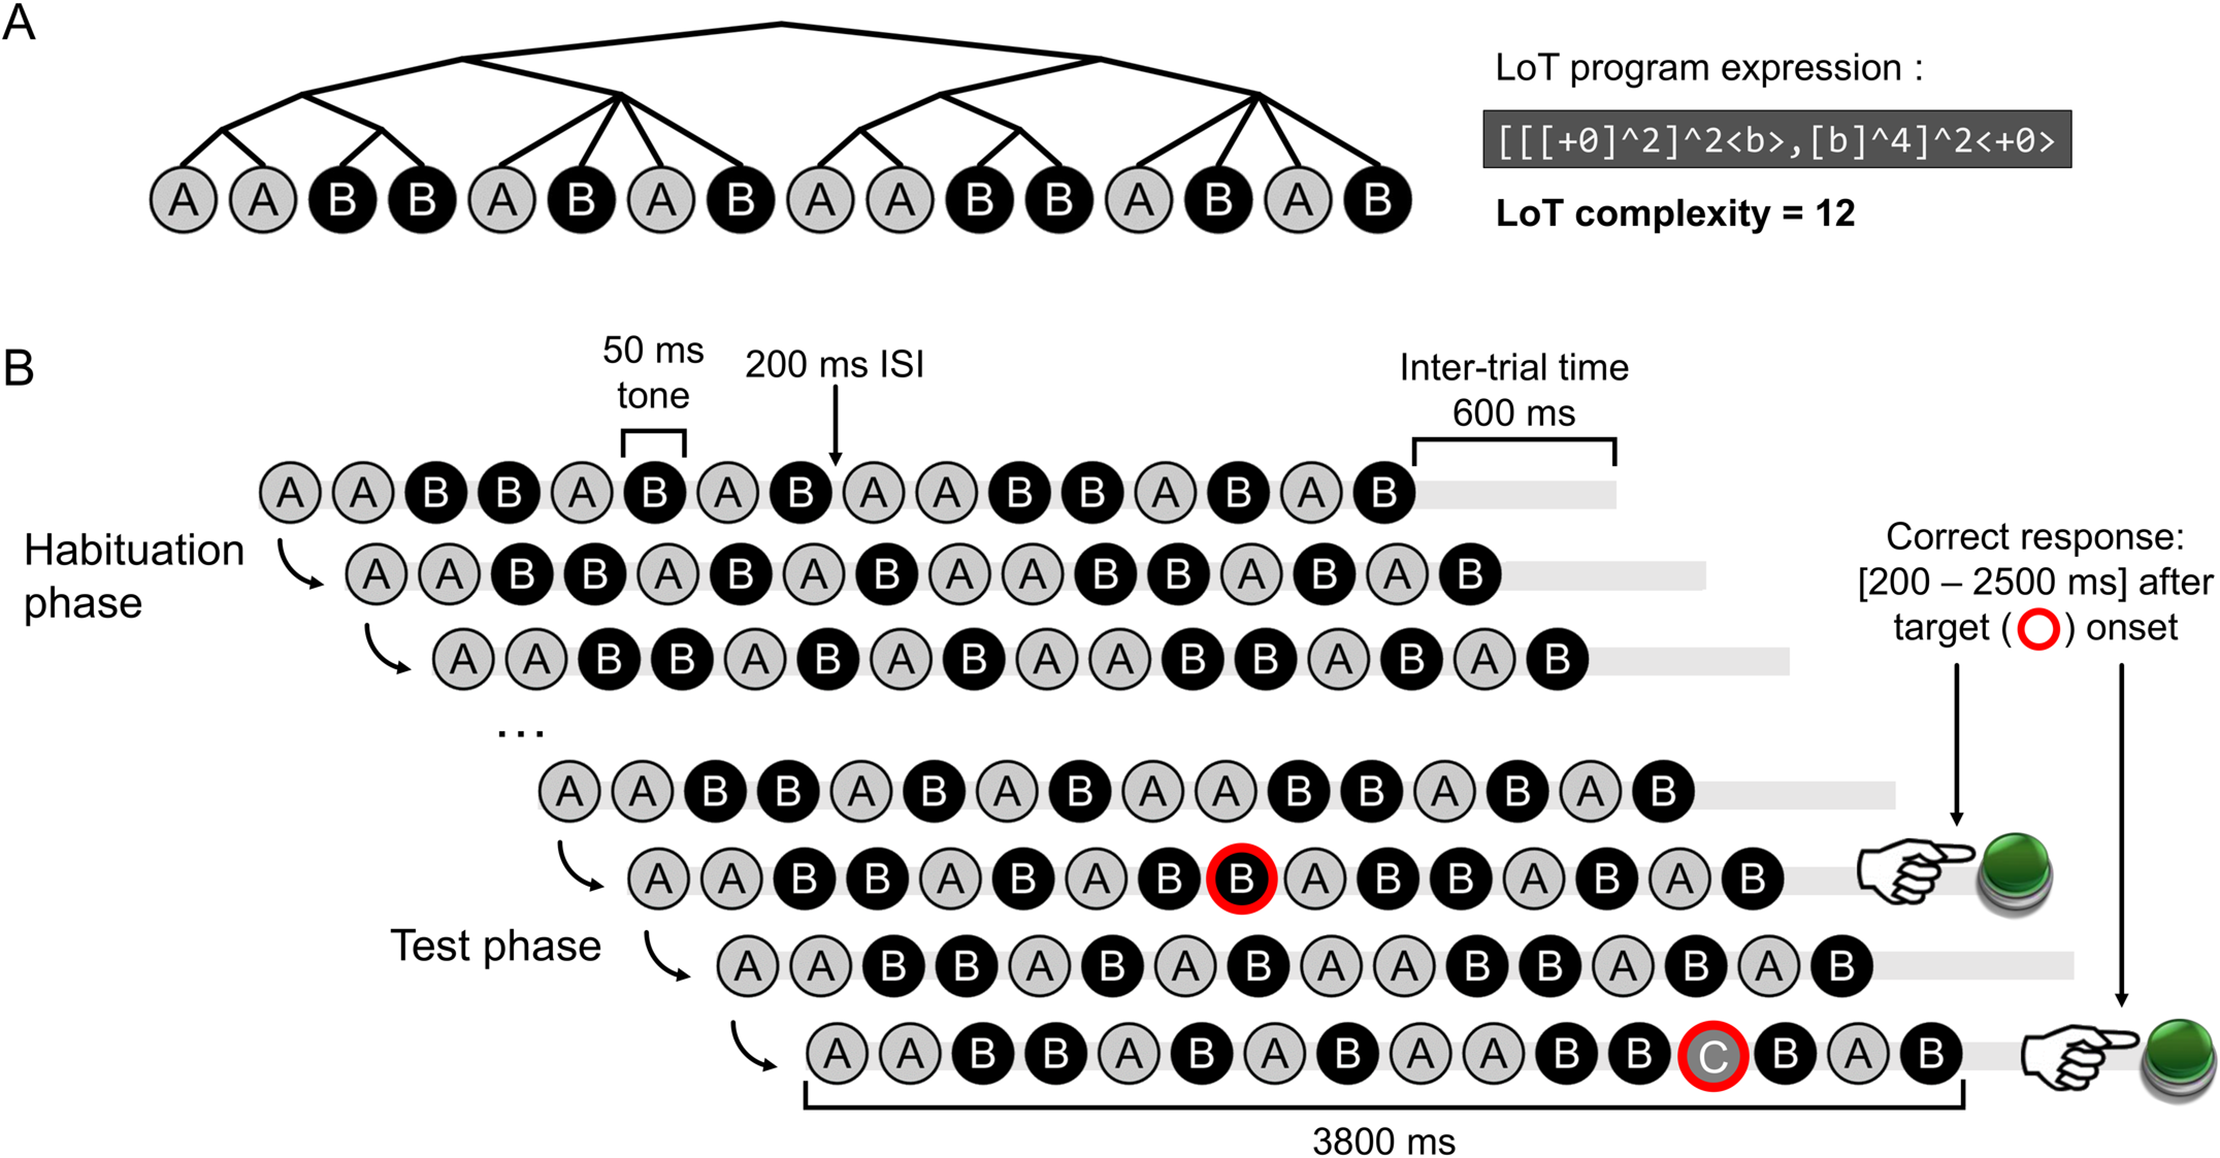
\includegraphics[scale=0.8]{journal.pcbi.1008598.g001.PNG}
   
   \centering
   %Figure 1: (A) Example of a 16-items long sequential pattern, with its shortest representation in the language of thought (i.e. LoT program expression) and the tree-structure derived from this expression (illustrating the hierarchical representation). The LoT complexity of this sequence is also indicated. (B) Experimental design of the violation detection task: a session with the sequence AABBABABAABBABAB is represented, with one example target deviant item (“A” replaced by “B”, at position 9) and one example target súper-deviant item (“C” at position 13). Deviants could occur at positions 9, 11, 13 or 15.
   
   \caption{(A) Ejemplo de un patrón de secuencia larga de 16 elementos, con su representación más corta en el LoT (es decir, la expresión del programa LoT) y la estructura de árbol derivada de esta expresión (que ilustra la representación jerárquica). También se indica la complejidad de LoT de esta secuencia. (B) Diseño experimental de la tarea de detección de violaciones: se representa una sesión con la secuencia AABBABABAABBABAB, con un ejemplo de elemento desviado objetivo (A reemplazado por B, en la posición 9) y un ejemplo de elemento súper-desviador objetivo (C en la posición 13). Las desviaciones podían ocurrir únicamente en las posiciones 9, 11, 13 o 15}
   \label{PlosBIO-F1}
\end{figure}
\sergio{la figura no está traducida}  

\begin{figure}[t!]
   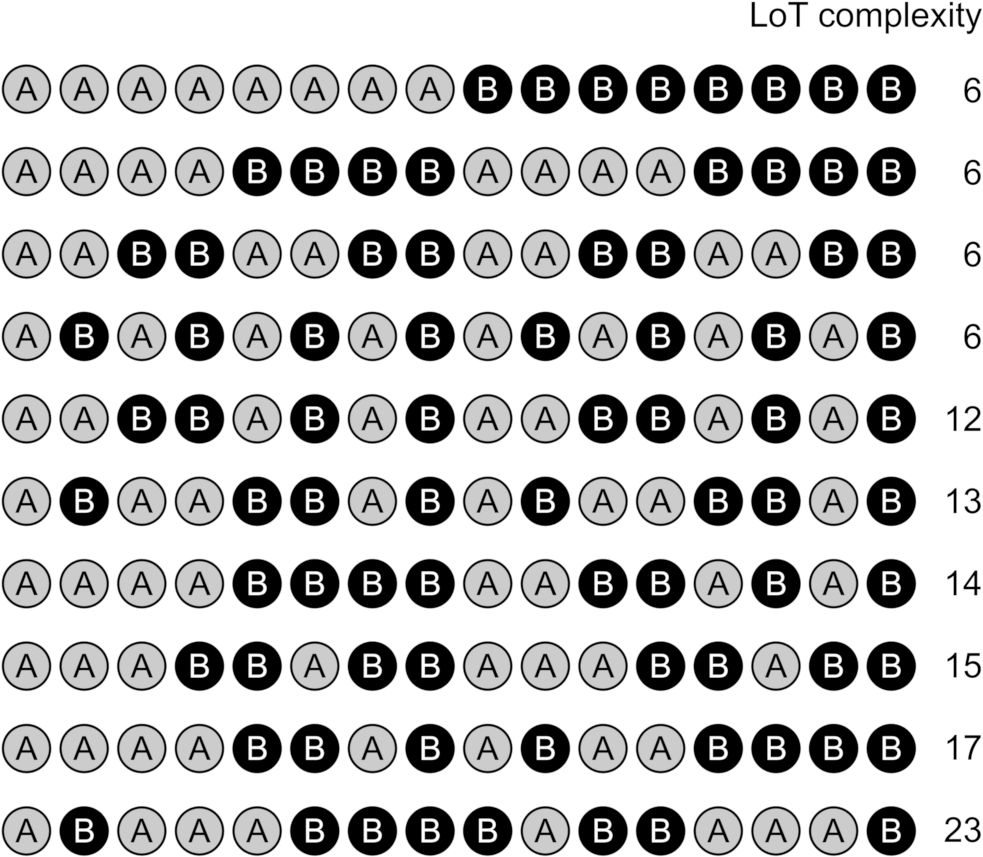
\includegraphics[scale=1]{journal.pcbi.1008598.g002.PNG}
   \centering
   %Ten 16-items long sequential patterns used in experiment 1, with their corresponding LoT complexity value.
   \caption{Diez patrones de secuencias largas de 16 elementos usados en el experimento 1, con su correspondiente valor de complejidad de LoT}
   \label{PlosBIO-F2}
\end{figure}
\sergio{la figura no está traducida}

\subsubsection*{Tarea de calificación de complejidad}

%We observed a strong positive linear relationship between average subjective complexity ratings and LoT complexity (entered as a fixed factor in the linear mixed model including participants as the random factor: t(278) = 24.6, p < .0001; Pearson correlation coefficient on the average ratings for each sequence: r = .94) (see Figure 3A). These results indicate that participants were readily able to judge whether a pattern is “more complex” than another, and that the formal language we used to compute sequence complexity is close to how individuals form such complexity judgements.

Se observó una fuerte relación lineal positiva entre la complejidad subjetiva promedio reportada y la complejidad LoT (introducida como un factor fijo en el modelo mixto lineal que incluye participantes como el factor aleatorio: $t (278) = 24.6, p < 0,0001;$ coeficiente de correlación de Pearson en las calificaciones promedio para cada secuencia: $r = .94$) \santi{unificar 0.X vs 0,X (punto vs coma)}(ver Figura~\ref{PlosBIO-F3}A). Estos resultados indican que los participantes pudieron juzgar fácilmente si un patrón es ``más complejo'' que otro, y que el lenguaje formal que usamos para calcular la complejidad de la secuencia se acerca a cómo los individuos forman tales juicios de complejidad.

\subsubsection*{Efectos de tipo de desviación y complejidad en la tarea de detección de infracciones}

%We observed a linear relationship of LoT complexity and performance in the violation detection task (using the Linear Integrated Speed-Accuracy Score, LISAS, an integrated measure of response times and error rates, see 87,88). We observed main effects of LoT complexity (t(415.0) = 18.1, p < .0001), deviant type (994 ms for sequence deviants vs. 570 ms for súper-deviants; t(414.4) = 18.9, p < .0001) and their interaction (t(414.5) = 11.7, p < .0001). Indeed, the slope of the complexity effect was significantly stronger, by an order of magnitude, for sequence deviants as opposed to súper-deviants (respectively +51 ms vs. +5 ms in simple regression, t(16) = 11.7, p < .0001; see Figure 3B, and Fig. S1 for the corresponding results using response times or miss rate instead of LISAS). Nevertheless, separate analyses revealed that LoT complexity was a strong predictor of performance for sequence deviants (t(193.0) = 15.5, p < .0001; r = .98) and also, surprisingly, for súper-deviants (t(198.5) = 4.08, p < .0001; r = .72) (Figure 3B). The latter effect on LISAS was however mainly driven by response times, since the average hit-rate for súper-deviants was high (96\%) and weakly modulated by LoT complexity (t(200.7) = 2.32, p = .022).

Observamos una relación lineal entre la complejidad LoT y el rendimiento en la tarea de detección de violaciones (utilizando la medida \textit{linear integrated speed-accuracy score} (LISAS), una medida integrada de tiempos de respuesta y tasas de error, ver~\cite{f87,f88}). Hemos observado efectos principales de complejidad LoT ($t(415.0) = 18.1, p <0,0001$), tipo de desviación (994ms para desviaciones de secuencias vs. 570ms para súper-desviaciones; $t (414.4) = 18.9, p < .0001$) y su interacción ($t(414.5) = 11. 7, p < .0001$). De hecho, la pendiente del efecto de complejidad fue significativamente más fuerte, en un orden de magnitud, para las desviaciones de secuencia en comparación con las súper-desviaciones (respectivamente +51ms frente a +5ms en la regresión lineal, $t(16) = 11.7, p <0.0001$; consultar la Figura~\ref{PlosBIO-F3}B y la Figura~\ref{PlosBIO-F1} para los resultados correspondientes utilizando el tiempo de respuesta o la tasa de errores en lugar de LISAS). Sin embargo, análisis separados revelaron que la complejidad LoT era un fuerte predictor de rendimiento para la desviación de secuencias ($t(193.0) = 15.5, p <0.0001; r = 0.98$) y también, sorprendentemente, para súper-desviaciones ($t (198.5) = 4.08, p < .0001; r = .72$) (Figura~\ref{PlosBIO-F3}B). El último efecto en LISAS, sin embargo, fue impulsado principalmente por el tiempo de respuesta, ya que la tasa de éxito promedio para súper-desviaciones fue alta (96\%) y débilmente modulada por la complejidad LoT ($t(200.7) = 2.32, p = .022$).

%The number of false alarms per sequence (which was 1.99 on average) also increased with sequence LoT complexity (t(214.4)=4.20, p < .0001; r = .74), suggesting here again that the LoT complexity was a good predictor of the quality of sequence encoding.

El número de falsas alarmas\santi{se entiende qué es una falsa alarma?} por secuencia (que era 1.99 en promedio) también aumentó con la complejidad LoT de la secuencia ($t(214.4)= 4.20, p <0.0001; r = 0.74$), lo que sugiere de nuevo que la complejidad LoT es un buen predictor de la calidad de la codificación de secuencias.

%The results of this first experiment with long binary auditory sequences (16 items) thus indicate that the formal language used to describe sequences in a compressed form, based on simple (possibly embedded) rules, is highly relevant to predict (i) how “complex” an auditory sequence is judged by adult participants after having listened to it once and (ii) how difficult it was to learn these sequences in order to detect alterations. 

Los resultados de este primer experimento con secuencias binarias auditivas largas (16 elementos) indican, por lo tanto, que el lenguaje formal utilizado para describir la secuencia en una forma comprimida, basado en reglas simples con capacidad de ser embebidas\santi{embebidas es una mala traducción de embedding. Se refiere a anidadas?}, es de gran importancia para predecir (i) cuán ``compleja'' una secuencia auditiva es juzgada por los participantes adultos después de haberla escuchado una vez y (ii) lo difícil que fue aprender estas secuencias para que puedan detectar alteraciones.

%Sequence complexity was expected to have little or no impact on the detection of súper-deviants, i.e. high or low pitch tones different from the two tones composing the binary auditory sequence. Our rationale was that such “C” tones were detectable even without any prior knowledge of sequence structure. While performance in detecting súper-deviants was much better than for sequence deviants, even for the simplest sequences, a clear relationship between LoT complexity and performance continued to be observed. We see at least two interpretations of this finding. First, there could be an increased attentional cost of having to detect violations in more complex sequences, thus placing subjects in a dual-task setting of having to simultaneously maintain a complex representation in memory and to respond to deviants. Alternatively, the effect could reflect the influence of a top-down prediction system which would use sequence structure to generate predictions of the incoming stimuli. Complex sequences would be less well predicted, and this would in turn affect the speed with which any deviant is detected. We return to this question in the General Discussion.

Se esperaba que la complejidad de la secuencia tenga poco o ningún impacto en la detección de súper-desviadaciones, (tonos altos o bajos diferentes de los dos tonos que componen la secuencia auditiva binaria). Nuestro razonamiento fue que esos tonos C eran detectables incluso sin ningún conocimiento previo de la estructura de la secuencia. Si bien el rendimiento en la detección de súper-desviaciones fue mucho mejor que para las desviaciones de secuencia, incluso para las secuencias más simples, se siguió observando una relación clara entre la complejidad LoT y el rendimiento. Vemos al menos dos interpretaciones de este hallazgo. Primero, podría haber un mayor costo de atención de tener que detectar violaciones en secuencias más complejas, colocando así a los sujetos en un entorno de una doble tarea de tener que mantener simultáneamente una representación compleja en la memoria y responder a las desviaciones. Alternativamente, el efecto podría reflejar la influencia de un sistema de predicción de arriba hacia abajo que usaría la estructura de secuencia para generar predicciones de los estímulos entrantes. Las secuencias complejas se predecirían peor y esto, a su vez, afectaría la velocidad con la que se detecta cualquier desviación. Volvemos a esta cuestión en la~\ref{chapter:BOI-GeneralDiscusion}.\santi{roto}

\subsubsection*{Efectos de sorpresa}\santi{Efectos sorpresa? EN TODO EL CAPITULO}

%Many prior experiments, using either or both behavior and brain-imaging measures, have shown that individuals constantly entertain predictions about future observations using probabilistic knowledge based on past observations (e.g. 19,20). In order to test whether task performance could be explained by a learning transition probabilities (surprise) only, or also truly implied an encoding of sequence structure, we compared a mixed model (with participants as a random effect) including fixed effects of both LoT complexity and surprise (averaged across the 4 possible positions of deviants in a given sequence) with a null model including only surprise. The effect of surprise in the null model with surprise alone) was significant (t(193.0) = 5.31, p < .0001). However, a likelihood ratio test showed that adding LoT complexity significantly improved the goodness of fit: χ²(1) = 130.9, p < .0001. Adding a “period” factor (i.e. period values were 2, 4, 8 or 16) as a third fixed effect did not improve the model fit (χ2(1) = 1.23, p = .267), confirming the prediction that the four included AnBn patterns have the same psychological complexity, and suggesting that this information is already captured by LoT complexity. Adding the interaction between surprise and LoT complexity did not improve goodness of fit either (χ2(1) = 2.50, p = .114). As reported in Table 1, the LoT complexity fixed effect was significant in the final full model (t(192.4) = 13.6, p < .0001), but not the surprise fixed effect (t(191.8) = 0.60, p = .55). The absence of a significant effect of surprise once sequence complexity is taken into account reflects the existence of a correlation between the two measures (r = –.54): biased transition probabilities in less complex sequences tending to make deviants more easily surprising. It also shows that when these two slightly colinear factors are included, LoT is more effective than surprise at describing the variance of the data.

Muchos experimentos previos, utilizando alguna o ambas medidas de comportamiento y de imagen cerebral, han demostrado que los individuos constantemente generan predicciones de futuras observaciones usando el conocimiento probabilístico basado en observaciones anteriores (por ejemplo,~\cite{f19,f20}). Para probar si el desempeño de la tarea podría explicarse sólo como un aprendizaje de la transición de probabilidad (sorpresa), o si también implicaba realmente una codificación de la estructura de la secuencia, comparamos un modelo mixto (con participantes como un efecto aleatorio) que incluye efectos fijos de complejidad LoT y sorpresa (promediada entre las 4 posibles posiciones de las desviaciones en una secuencia dada) con un modelo nulo que incluye sólo la sorpresa. El efecto de sorpresa en el modelo nulo con sorpresa sola fue significativo ($t(193.0) = 5.31, p < .0001$). Sin embargo, una prueba de razón de verosimilitud\santi{que es prueba de razón de verosimilitud?} mostró que agregar la complejidad LoT mejoraba significativamente la bondad de ajuste: $\chi^2(1) = 130.9, p < .0001$. Agregar un factor de ``período'' (los valores del período fueron 2, 4, 8 o 16) como un tercer efecto fijo no mejoró el ajuste del modelo ($\chi^2(1) = 1.23, p = .267$), lo que confirma la predicción de que los cuatro patrones $A^n B^n$ incluidos tienen la misma complejidad subjetiva, y sugiere que esta información ya está capturada por la complejidad LoT. La adición de la interacción entre la sorpresa y la complejidad LoT tampoco mejoró la bondad del ajuste ($\chi^2(1) = 2.50, p = . 114$). Como se informa en la Tabla~\ref{PlosBIO-T1}, el efecto fijo de la complejidad LoT fue significativo en el modelo completo final ($t(192.4) = 13.6, p < .0001$), pero no el efecto fijo de la sorpresa ($t (191.8) = 0.60, p = .55$). La ausencia de un efecto de sorpresa significativo una vez que se tiene en cuenta la complejidad de la secuencia refleja la existencia de una correlación entre las dos medidas ($r = -.54$): probabilidades de transición sesgadas en secuencias menos complejas tienden a hacer que las desviaciones sean más fácilmente sorprendentes. También muestra que cuando se incluyen dos factores con una pequeña colinealidad, LoT es más eficaz que la sorpresa en la descripción de la varianza de los datos.

%As our choice of attributing an arbitrary padding value (0.01) to deviant transitions events with zero probability when computing surprise may have biased the results, we recomputed the LISAS and average surprise while excluding all such trials (i.e. all deviant positions in the (AB)8 pattern, 3 out of 4 deviant positions in the A8B8 pattern). Here again, a likelihood ratio test showed that the goodness of fit increased significantly when adding LoT complexity to a null model containing only surprise (χ²(1) = 116.3, p < .0001). However, both complexity (t(165.5) = 12.9, p < .0001) and surprise (t(165.8) = 3.82, p < .0001) were significant with this subset of the data.

Como nuestra elección de atribuir valor arbitrario de relleno (0.01) a los eventos de transición de desviaciones con probabilidad cero al calcular la sorpresa puede haber sesgado los resultados, recomputamos la medida LISAS y la media de la sorpresa excluyendo todos esos ensayos (es decir, todas las posiciones de desviación en el patrón $(AB)^8$ y 3 de 4 posiciones de desviación en el patrón $A^8 B^8$).\santi{está definido este exponente?} Aquí nuevamente, una prueba de razón de verosimilitud mostró que la calidad del ajuste aumentó significativamente cuando se agregó la complejidad LoT a un modelo nulo que sólo contenía sorpresa ($\chi^2(1) = 116.3, p < .0001$). Sin embargo, tanto la complejidad ($t (165.5) = 12.9, p < .0001$) como la sorpresa (t ($165.8) = 3.82, p < .0001$) fueron significativas con este subconjunto de datos. \sergio{entender efecto de relleno explicado}\santi{si, por favor ;)}

%In conclusion, the strong complexity effects observed here indicated that participants used some form of compression of information to encode the sequence and perform the task over and above simply learning statistical trends. Although no instruction was given in that sense, this strategy may be needed in order to deal with a difficult, memory-demanding task. Indeed, at the maximum level of complexity used, performance in violation detection was very low (the violation detection rate dropped to 41% for sequence deviants).

En conclusión, los fuertes efectos de complejidad observados indicaron que los participantes usan alguna forma de compresión de la información para codificar la secuencia y realizar la tarea más allá de simplemente aprender tendencias estadísticas de los elementos. Aunque no se dio ninguna instrucción en ese sentido, esta estrategia puede ser necesaria para hacer frente a una tarea difícil que exige memoria. De hecho, en el nivel máximo de complejidad utilizado, el rendimiento en la detección de violaciones fue muy bajo (la tasa de detección de violaciones se redujo al 41\% para las desviaciones de secuencias).

%In the subsequent experiments, we asked whether similar complexity effects emerged in the same paradigm but with shorter sequences. That is, when the sequence can be more easily encoded and stored “as a whole”, without necessarily requiring a re-encoding in a more abstract, compressed form. In these less demanding conditions, it can be expected that the spontaneous encoding of transitions probabilities between items will play a more important role in the detection of violations.

En los experimentos posteriores, nos preguntamos si los efectos de complejidad similares pueden ser vistos en el mismo paradigma, pero con secuencias más cortas. Es decir, cuando la secuencia se puede codificar y almacenar más fácilmente ``en su conjunto'', sin que se requiera necesariamente una recodificación en una forma más abstracta o comprimido.\santi{revisar redaccion de Es decir,...} En estas condiciones menos exigentes, se puede esperar que la codificación espontánea de las probabilidades de transición entre elementos juegue un papel más importante en la detección de violaciones.

\begin{figure}[t!]
   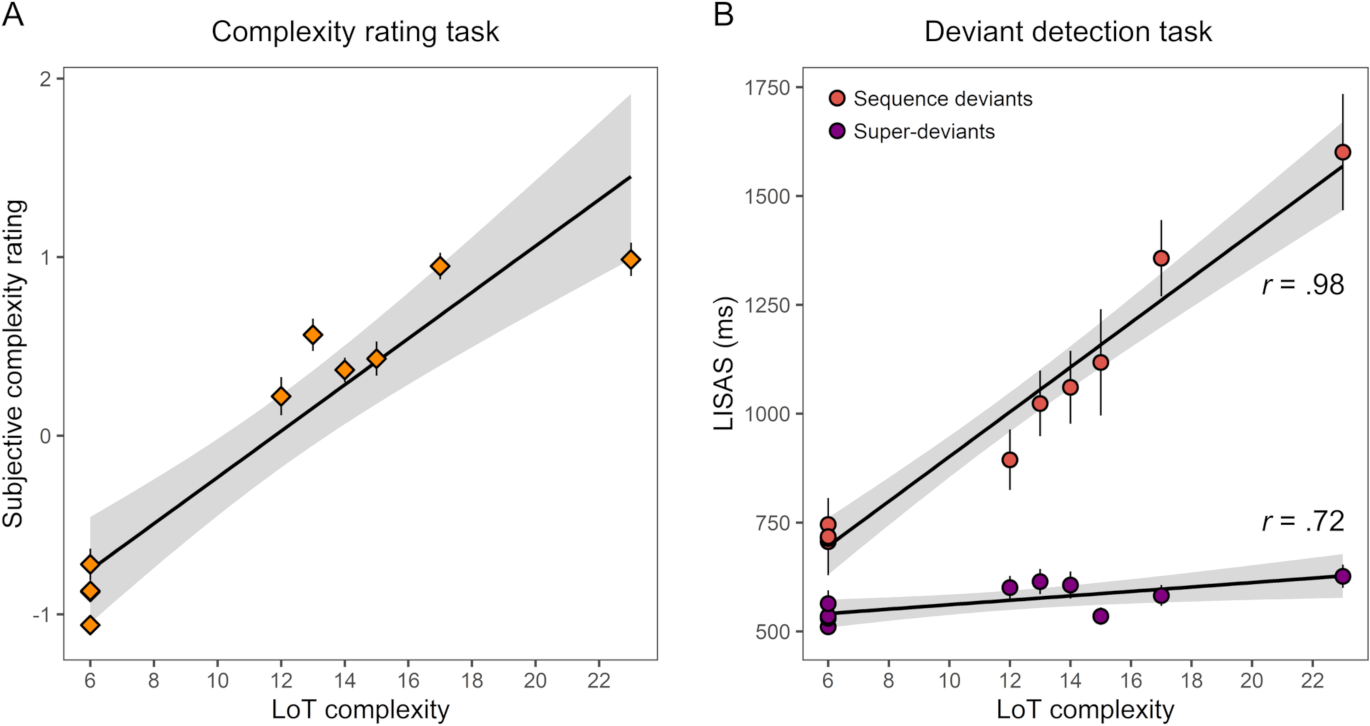
\includegraphics[scale=1]{journal.pcbi.1008598.g003.PNG}
   \centering
   %Linear relationship between LoT complexity and subjective and objective measures obtained in experiment 1 with ten 16-items long auditory sequences (with 95% confidence intervals bands in gray). The Pearson correlation coefficient (r) is indicated. Each marker represents the group-average for a given sequence. Error bars represent SEM across participants. (A) LoT complexity vs. subjective complexity ratings. (B) LoT complexity vs. performance in the violation detection task (Linear Integrated Speed-Accuracy Score), for sequence deviants and súper-deviants.
   \caption{Relación lineal entre la complejidad LoT y las medidas subjetivas y objetivas obtenidas en el experimento 1 con diez secuencias auditivas largas de 16 elementos (intervalos de confianza del 95\% en gris). El coeficiente de correlación de Pearson ($r$) aparece indicado. Cada marcador representa el promedio del grupo para una determinada secuencia. Las barras de error representan el s.e.m. entre los participantes. (A) Clasificación de complejidad LoT frente a complejidad subjetiva. (B) Complejidad LoT frente a rendimiento en la tarea de detección de violaciones (medida integrada de tiempos de respuesta y tasas de error, LISAS), para desviaciones de secuencia y súper-desviaciones.}
   \label{PlosBIO-F3}
\end{figure}
\sergio{la figura no está traducida}

\santi{que es pag en la tabla?}
\begin{table}[]
\centering
\begin{tabular}{lccccc}
\multicolumn{6}{l}{\textbf{Experimento 1} (secuencias de 16 elementos, excluyendo súper-desviados)}                          \\ \hline
\textit{Predictores}     & \textit{Estimados}  & \textit{Std. Error} & \textit{Valor t}   & \textit{IC del 95\%} & \textit{pag}       \\ \hline
(Interceptar)         & 356,90        & 80,51        & 4.43         & 199,5 - 514,3    & \textbf{\textless{}.0001} \\
Complejidad          & 52.15        & 3,84         & 13.60        & 44,6 - 59,7     & \textbf{\textless{}.0001} \\
Sorpresa           & 6,77         & 11.31        & 0,60         & -15,4 - 28,9     &.55            \\ \hline
\multicolumn{1}{c}{}     & \multicolumn{1}{l}{} &           &           &           &              \\
\multicolumn{6}{l}{\textbf{Experimento 2} (secuencias de 12 elementos, excluyendo súper-desviados)}                          \\ \hline
\textit{Predictores}     & \textit{Estimados}  & \textit{Std. Error} & \textit{Valor t}   & \textit{IC del 95\%} & \textit{pag}       \\ \hline
(Interceptar)         & 852,38        & 124,91        & 6,82         & 608,5 - 1096,2    & \textbf{\textless{}.0001} \\
Complejidad          & 24,21        & 6.29         & 3,85         & 11,9 - 36,5     & \textbf{\textless{}.0002} \\
Sorpresa           & -43,13        & 21.06        & -2.05        & -84,4 - -1,9     & \textbf{\textless{}.05}  \\ \hline
\textbf{}           & \multicolumn{1}{l}{} & \multicolumn{1}{l}{} & \multicolumn{1}{l}{} & \multicolumn{1}{l}{} & \multicolumn{1}{l}{}   \\
\multicolumn{6}{l}{\textbf{Experimento 3} (secuencias de 8 elementos)}                                        \\ \hline
\textit{Predictores}     & \textit{Estimados}  & \textit{Std. Error} & \textit{Valor t}   & \textit{IC del 95\%} & \textit{pag}       \\ \hline
(Interceptar)         & 852.40        & 73,39        & 11,62        & 707,8 - 997     & \textbf{\textless{}.0001} \\
Complejidad          & 10,75        & 3,49         & 3,08         & 3,9 - 17,6      & \textbf{\textless{}.003} \\
Sorpresa           & -32,37        & 5.60         & -5,78        & -43,3 - -21,4    & \textbf{\textless{}.0001} \\ \hline
\multicolumn{1}{c}{\textbf{}} & \multicolumn{1}{l}{} & \multicolumn{1}{l}{} & \multicolumn{1}{l}{} & \multicolumn{1}{l}{} & \multicolumn{1}{l}{}   \\
\multicolumn{6}{l}{\textbf{Experimento 4} (secuencias de 6 elementos, secuencia 'AAAAAA' excluida)}                          \\ \hline
\textit{Predictores}     & \textit{Estimados}  & \textit{Std. Error} & \textit{Valor t}   & \textit{IC del 95\%} & \textit{pag}       \\ \hline
(Interceptar)         & 751,6        & 47,5         & 15,8         & 658,8 - 844,5    & \textbf{\textless{}.0001} \\
Complejidad          & 1.4         & 4.4         & 0,3         & -7,2 - 9,9      &.75            \\
Sorpresa           & -15,3        & 3.8         & -4,1         & -22,7 - -7,9     & \textbf{\textless{}.0001} \\ \hline
\multicolumn{1}{c}{\textbf{}} & \multicolumn{1}{l}{} & \multicolumn{1}{l}{} & \multicolumn{1}{l}{} & \multicolumn{1}{l}{} & \multicolumn{1}{l}{}   \\
\multicolumn{6}{l}{\textbf{Experimento 5} (secuencias de 8 ítems, auditivo y visual)}                                 \\ \hline
\textit{Predictores}     & \textit{Estimados}  & \textit{Std. Error} & \textit{Valor t}   & \textit{IC del 95\%} & \textit{pag}       \\ \hline
(Interceptar)         & 645,1        & 92,2         & 7.0         & 464,4 - 825,9    & \textbf{\textless{}.0001} \\
Complejidad          & 25,2         & 25,2         & 4.4         & 14 - 36,4      & \textbf{\textless{}.0001} \\
Sorpresa           & -36,7        & 8.1         & -4,5         & -52,5 - -20,8    & \textbf{\textless{}.0001} \\
Modalidad (visual)      & 337,0        & 337,0        & 14,2         & 290,7 - 383,3    & \textbf{\textless{}.0001} \\ \hline
\end{tabular}
\caption{Efectos fijos en los modelos lineales mixtos, separados para cada experimento}
\label{PlosBIO-T1}
\end{table}

\subsection{Experimento 2: secuencias auditivas con 12 elementos}
\label{ploscomp-results-exp2}

%In order to test whether the previous results could be replicated with shorter sequences, in experiment 2, the same tasks and procedure were used (with a different group of participants), this time using twelve sequences of twelve items (spanning a large range of complexities, see Figure 4).

Para probar si los resultados anteriores podían replicarse con secuencias más cortas, en el experimento 2, se utilizaron las mismas tareas y el mismo procedimiento (con un grupo diferente de participantes), pero esta vez usando doce secuencias de doce elementos (que abarcan una amplia gama de complejidades, vea la Figura~\ref{PlosBIO-F4}).

\begin{figure}[t!]
   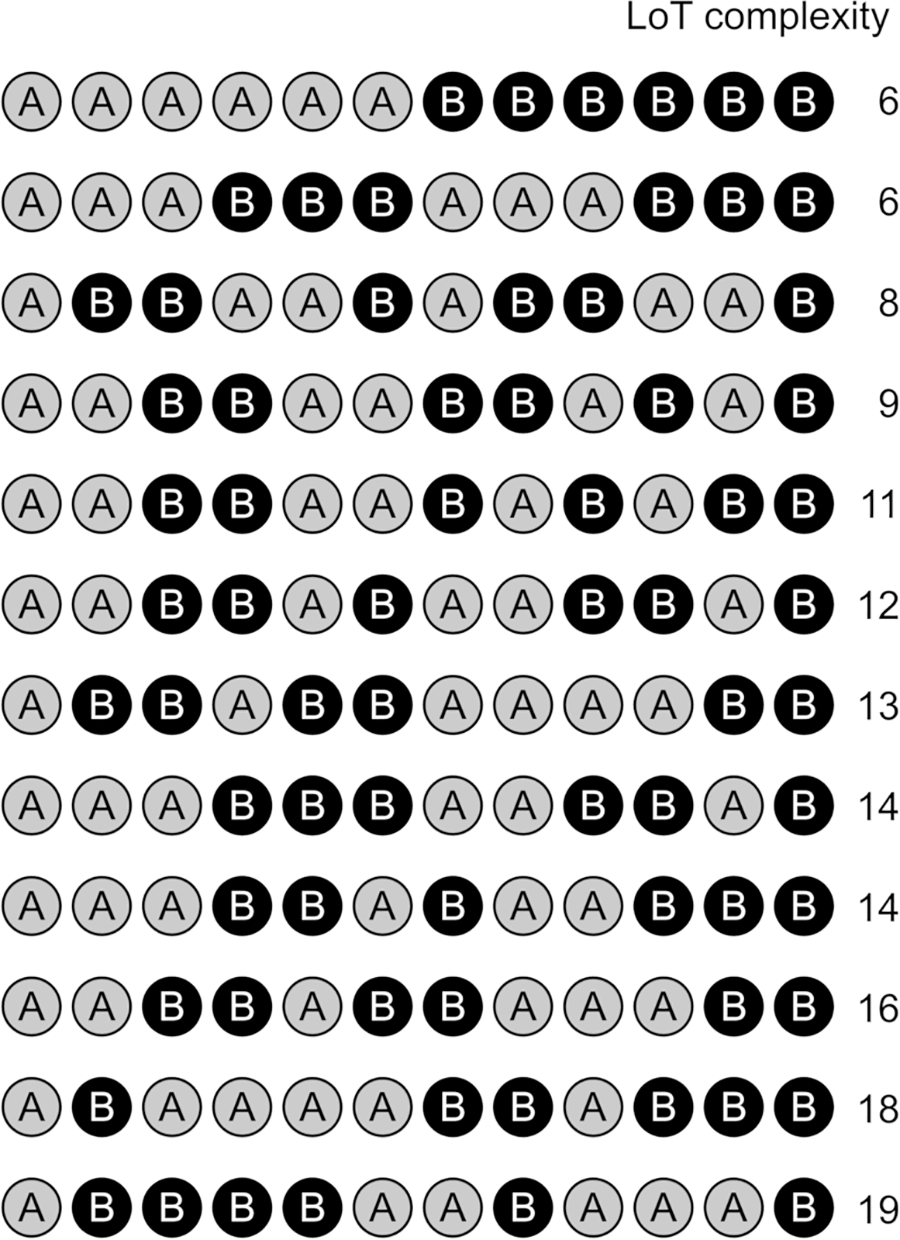
\includegraphics[scale=1]{journal.pcbi.1008598.g004.PNG}
   \centering
   %Twelve 12-item sequences used in experiment 2, with their corresponding LoT complexity value (in bits).
   \caption{Doce secuencias de 12 elementos utilizadas en el experimento 2, con su correspondiente valor de complejidad LoT (en bits)}
   \label{PlosBIO-F4}
\end{figure}
\sergio{la figura no está traducida}

\subsubsection*{Tarea de calificación de complejidad}

%A positive linear relationship was found between subjective complexity ratings and LoT complexity (t(238) = 6.81 p < .0001, r = .61). The correlation of the average score per sequence with LoT complexity was however less strong than what was observed in the previous experiment with 16-items long sequences (r = .61, see Figure 5A). Subjective complexity was clearly underestimated for one specific sequence (ABBAABABBAAB, predicted complexity of 8), which is confirmed by an inspection of the residuals of the regression (residual 1.99 SD above average for this sequence).

Se encontró una relación lineal positiva entre los reportes de complejidad subjetiva y la complejidad LoT ($t(238) = 6.81 p < .0001, r = .61$). La correlación de la complejidad subjetiva media por secuencia con la complejidad LoT era, sin embargo, menos fuerte que lo observado en el experimento anterior con 16 secuencias largas de 16 elementos ($r = .61$, ver Figura~\ref{PlosBIO-F4}A). La complejidad subjetiva estuvo claramente subestimada para una secuencia específica (ABBAABABBAAB, con una complejidad predicha de 8), lo cual se confirma con una inspección de los residuos de la regresión (residual 1.99 SD por encima del promedio para esta secuencia).

%Deviant type and complexity effects in the violation detection task
\subsubsection*{Tipos de desviaciones y efectos de la complejidad en la tarea de detección de violaciones}

%Regarding the violation detection task, main effects of LoT complexity (t(431.1) = 6.43, p < .0001) and deviant type (1078 ms for sequence deviants vs. 545 ms for súper-deviants; t(431.0) = 19.3, p < .0001) were observed, as well as their interaction (t(431.1) = 3.48, p < .001). The slope of the complexity effect appeared indeed slightly stronger for sequence deviants as opposed to súper-deviants, although the comparison did not reach significance when using simple linear regressions with averaged LISAS per sequence (slopes of respectively +30 ms vs. +7 ms, t(20) = 1.87, p = .077; see Figure 5B, and Fig. S2 for the corresponding results with RTs and miss rates instead of LISAS). Separated analyses revealed that the effect of LoT complexity was significant in analyses restricted to either sequence deviants (t(205.1) = 5.78, p < .0001; r = .63), or súper-deviants (t(208.0) = 2.88, p = .005; r = .59) only. The number of false alarms per sequence (3.88 on average) was also significantly predicted by the LoT complexity of the sequence (t(208.0) = 3.50, p < .001; r = .56).

\santi{chequear redaccion de Con respecto a...}Con respecto a la tarea de detección de violaciones, los principales efectos de la complejidad LoT ($t (431.1) = 6.43, p < .0001$) y el tipo de desviación (1078 ms para desviaciones de secuencia vs 545 ms para súper-desviaciones; $t (431.0) = 19.3, p < .0001$), así como su interacción ($t (431.1) = 3.48, p < .001$). La pendiente del efecto de complejidad apareció de hecho ligeramente más fuerte para las desviaciones de secuencia en comparación con las súper-desviaciones, aunque la comparación no fue significativa cuando se usaron regresiones lineales simples con LISAS promediado por secuencia (pendientes de +30 ms frente a +7 ms, respectivamente, $t (20) = 1.87, p = .077$; consultar la Figura~\ref{PlosBIO-F5}B y la Figura~\ref{PlosBIO-F2} para obtener los resultados correspondientes con tiempo de respuesta y tasas de error en lugar de LISAS). Los análisis separados revelaron que el efecto de la complejidad LoT fue significativo en los análisis restringidos a secuencias con desviaciones ($t (205.1) = 5.78, p < .0001; r = .63$), o súper-desviaciones ($t (208.0) = 2.88, p = .005; r = .59$) solamente. El número de falsas alarmas por secuencia (3.88 en promedio) también fue predicho significativamente por la complejidad LoT de la secuencia ($t (208,0) = 3,50, p < .001; r = .56$).

%As in the complexity rating task, although the overall correlation was high, a noticeable deviation between predicted complexity and observed performance was present for some of the sequences. In fact, the correlation profiles observed in the Figure 5A and 5B suggest that the psychological complexity of the pattern, as indexed by subjective rating or violation detection task performance, might have been, for some sequences, consistently overestimated or underestimated by the LoT across both tasks (the largest residual in the regression with the sequence deviants, 1.50 SD above average, corresponded to the same sequence identified by complexity ratings: ABBAABABBAAB). To further test this idea, we computed the correlation between the residuals of both linear regressions. The correlation was significant (t(10) = 4.02; p = .003), indicating that even after regressing out the effect of LoT complexity, the data from both experiments remained correlated with each other, and thus that, although the proposed LoT is a good predictor, it does not fully account for all details of the psychological complexity of patterns. One attempt to address the limitations of the language, by proposing a modification of it, is reported in the Further analysis section.

Al igual que en la tarea de calificación de complejidad, aunque la correlación general fue alta, hubo una desviación notable entre la complejidad predicha y el rendimiento observado para algunas de las secuencias. De hecho, los perfiles de correlación observados en la Figura~\ref{PlosBIO-F5}A y la Figura~\ref{PlosBIO-F5}B sugieren que la complejidad psicológica del patrón, según lo indexado por la calificación subjetiva o el desempeño de la tarea de detección de violaciones, podría haber sido para algunas secuencias constantemente sobrestimado o subestimado por el LoT en ambas tareas (el residuo más grande en la regresión con las desviaciones de secuencia, 1.50 SD por encima del promedio, correspondió a la misma secuencia identificada por la clasificación de complejidad subjetiva: ABBAABABBAAB). Para probar más esta idea, calculamos la correlación entre los residuos de ambas regresiones lineales. La correlación fue significativa ($t (10) = 4.02; p = .003$), lo que indica que --incluso después de hacer una regresión del efecto de la complejidad LoT-- los datos de ambos experimentos permanecieron correlacionados entre sí y, por lo tanto, aunque el LoT propuesto es un buen predictor, no explica por completo todos los detalles de la complejidad psicológica de los patrones. Un intento de abordar las limitaciones del lenguaje, proponiendo una modificación, se informa en la sección~\ref{PlosBIO-AnalisisAdiocional}.\santi{roto}

\begin{figure}[t!]
   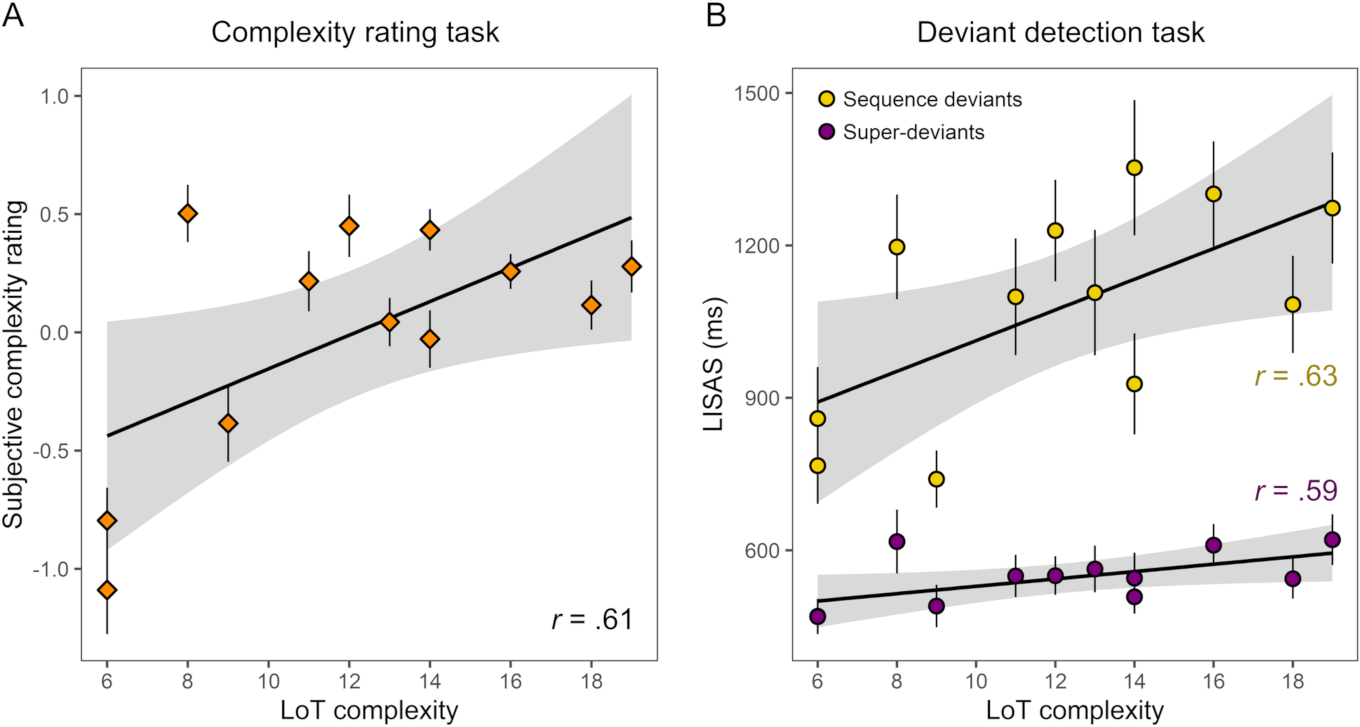
\includegraphics[scale=1]{journal.pcbi.1008598.g005.PNG}
   \centering
   %Linear relationship between LoT complexity and scores obtained in the two tasks of experiment 2 with 12-item auditory sequences (with 95% confidence intervals bands in gray). Same format as Figure 3.
   \caption{Relación lineal entre la complejidad LoT y las puntuaciones obtenidas en las dos tareas del experimento 2 con secuencias auditivas de 12 elementos (con bandas de intervalos de confianza del 95\% en gris). Mismo formato que la Figura~\ref{PlosBIO-F3}}
   \label{PlosBIO-F5}
\end{figure}
\sergio{la figura no está traducida}

\subsubsection*{Efectos de sorpresa}
%A comparison of mixed models (with participants as a random effect) showed that, compared to a null model including surprise as the sole predictor (null model; in which the main predictor was significant: t(205.0) = 4.67, p < .0001), a model additionally including LoT complexity (full model) fitted the data better (likelihood ratio test : χ²(1) = 14.4, p < .001). Both fixed effects were significant in the full model: LoT complexity (t(204.1) = 3.85, p < .0001), as well as surprise (t(204.0) = 2.05, p = .042) (see Table 1). Although we observed, contrary in the previous experiment, an effect of statistical learning (indexed by the level of surprise of deviant items), it was only barely statistically significant.

Una comparación de modelos mixtos (con participantes como el efecto aleatorio) \santi{redacción EN TODO EL CAPITULO: con participantes como el efecto aleatorio vs con participantes como un efecto aleatorio vs con participantes como efecto aleatorio} mostró que, en comparación con un modelo nulo que incluye la sorpresa como único predictor (modelo nulo en el que el predictor principal fue significativo: $t (205,0) = 4,67, p <0,0001$), un modelo que incluye adicionalmente la complejidad LoT (modelo completo) explica mejor los datos (prueba de razón de verosimilitud: $\chi^2(1) = 14.4, p < .001$). Ambos efectos fijos fueron significativos en el modelo completo: complejidad LoT ($t (204.1) = 3.85, p < .0001$), así como la sorpresa ($t (204.0) = 2.05, p= .042$) (ver Tabla~\ref{PlosBIO-T1}). \santi{redacción: Aunque hemos observado...}Aunque hemos observado, al contrario que en el experimento anterior, un efecto de aprendizaje estadístico (indexado por el nivel de la sorpresa del elemento desviado), que era sólo apenas estadísticamente significativo.

\subsection{Experimento 3 y 4: secuencias auditivas con 6 u 8 elementos}

%Results of experiments 1 and 2 showed that our sequence complexity metric was well correlated with behavior, suggesting that our formal language provided a good approximation of the internal language of thought that humans use to encode a sequence in memory a compressed from. These results were however obtained with a restricted set of sequences, which were long enough to promote hierarchical representations based on the repetition and alternation operations, and to probe a large range of complexity values. The main objective of experiments 3 (with 35 8-items long sequences, see Fig. S3) and 4 (with 32 6-items long sequences, see Fig. S4) was to test whether the effect of complexity observed in the first two experiments could be generalized to a larger set of shorter sequences, where we could examine more gradual variations in complexity. Given that human working memory is thought to store and maintain 4 to 7 items without compression, or with a minimal chunking process (25,29), we expected the predictive power of our language to be reduced compared with previous experiments with longer sequences, while the effects of transition probabilities would increase. The same violation detection paradigm was used. No subjective complexity ratings were collected (given the larger number of individual sequences compared to the previous experiments). 

Los resultados de los experimentos 1 y 2 mostraron que nuestra métrica de complejidad de secuencia se correlacionaba bien con el comportamiento, lo que sugiere que nuestro lenguaje formal proporcionó una buena aproximación del lenguaje interno del pensamiento que los humanos usan para codificar una secuencia comprimida en la memoria. Sin embargo, estos resultados se obtuvieron con un conjunto restringido de secuencias, que eran lo suficientemente largas para promover representaciones jerárquicas basadas en las operaciones de repetición y alternancia, y para probar una amplia gama de valores de complejidad. El objetivo principal del experimento 3 (con 35 secuencias largas de 8 elementos,\santi{no se entiende lo de largas de 8 o largas de 6} ver Figura~\ref{PlosBIO-F3}) y del experimento 4 (con 32 secuencias largas de 6 elementos, ver Figura~\ref{PlosBIO-F4}) fue probar si el efecto de la complejidad observado en los dos primeros experimento podría ser generalizados a un conjunto más amplio de secuencias más cortas,\santi{aclarar a qué se refiere con cortas y largas} en donde podamos examinar variaciones más graduales de la complejidad. Dado que la memoria de trabajo humana está pensada para almacenar y mantener de 4 a 7 elementos sin compresión, o con un proceso de agrupamiento mínimo (\cite{f25,f29}), esperamos que le poder predictivo de nuestro LoT se reduzca en comparación con los experimentos anteriores realizados con secuencias más largas, mientras que los efectos de las transiciones de probabilidad aumenten. Utilizamos en estos experimentos el mismo paradigma de detección de violaciones. No se recopilaron calificaciones de complejidad subjetiva (dado el mayor número de secuencias individuales en comparación con los experimentos anteriores).

%Here again, we tested (using mixed models) whether surprise suffices to explain the variance in performance or if a significant proportion of variance remained yet to be explained by sequence complexity (all models included participants as a random effect). In experiment 3 (8-items sequences, N = 35), goodness of fit improved when LoT complexity was included in the model (χ²(1) = 9.47, p = .002). Both fixed effects were significant in the full model: LoT complexity (t(1042.0) = 3.08, p = .002; see Figure 6A, and Fig. S5), as well as surprise (t(1042.0) = 5.78, p < .0001) (see Table 1). Note that the surprise fixed effect was already highly significant in the null model (t(1043.0) = 8.72, p < .0001).

Una vez más, hemos testeado (utilizando modelos mixtos) si es suficiente la sorpresa para explicar la variación en el rendimiento o si una proporción significativa de la varianza se mantuvo aún para ser explicada por la complejidad de la secuencia (todos los modelos incluyen los participantes como efecto aleatorio). En el experimento 3 (secuencias de 8 elementos, N = 35), la calidad del ajuste mejoró cuando se incluyó la complejidad LoT en el modelo ($\chi^2(1) = 9.47, p= .002$). Ambos efectos fijos fueron significativos en el modelo completo: complejidad LoT ($t (1042.0) = 3.08, p <= .002$; ver Figura~\ref{PlosBIO-F6}A y Figura~\ref{PlosBIO-F5}), así como la sorpresa ($t (1042.0) = 5.78, p < .0001$) (ver Tabla~\ref{PlosBIO-T1}). Tener en cuenta que el efecto fijo de la sorpresa\santi{efecto de la sorpresa vs efecto sorpresa EN TODO EL CAPITULO} ya era muy significativo en el modelo nulo ($t (1043.0) = 8.72, p < .0001$).

%Similarly, in experiment 4 (6-items sequences, N = 32), goodness of fit improved when LoT complexity was included in the surprise-only null model (χ²(1) = 6.20, p = .013) with both fixed effects significant in the full model (LoT complexity: t(649.00) = 2.49, p = .013; see Figure 6B, and Fig. S6), and surprise (t(649.0) = 5.48, p < .0001). The surprise fixed effect was here again already highly significant in the null model (t(650.0) = 6.78, p < .0001). However, one sequence appeared as an outlier in this experiment, with an average LISAS 3.9 SD below the average of all sequences (i.e. indicating a much better performance): the AAAAAA sequence. In this case, performing the task requires no sequence learning, but merely remembering the identity of the A sound, and violation detection is therefore similar to a classic oddball paradigm. When this sequence was removed from the dataset (it was also excluded from further analyses), the inclusion of the complexity fixed factor did no longer improved model goodness of fit (χ²(1) = 0.10, p = .752). Indeed, the LoT complexity fixed effect was not significant in the full model (t(628.0) = 0.32, p = .752), as opposed to the surprise fixed effect (t(628.0) = 4.07, p < .0001) (see Table 1). No improvement in model fit was found when including the interaction between complexity and surprise (χ²(1) = 0.08 in experiment 3, χ²(1) = 0.34 in experiment 4).

Del mismo modo, en el experimento 4 (secuencias de 6 elementos, N = 32), la calidad del ajuste mejoró cuando la complejidad LoT se incluyó en el modelo nulo con la sorpresa como único factor ($\chi^2(1) = 6.20, p= .013$) con ambos efectos fijos significativos en el modelo completo (complejidad LoT: $t (649.00) = 2.49, p= .013$; ver Figura~\ref{PlosBIO-F6}B y Figura~\ref{PlosBIO-F6}) y sorpresa ($t (649.0) = 5.4 8, p < .0001$). El efecto fijo de la sorpresa fue ya aquí otra vez altamente significativo en el modelo nulo ($t (650.0) = 6.78, p < .0001$). Sin embargo, una secuencia apareció como un valor atípico en este experimento, con un LISAS 3,9 SD promedio por debajo del promedio de todas las secuencias (es decir, indicando un rendimiento mucho mejor): la secuencia AAAAAA. En este caso, realizar la tarea no requiere un aprendizaje de secuencia, sino simplemente recordar la identidad del sonido A, y la detección de la violación es, por lo tanto, similar a un paradigma clásico de bichos raros\santi{se dice bichos raros en castellano?} (\textit{oddball}). Cuando esta secuencia se eliminó del conjunto de datos (también se excluyó de análisis posteriores), la inclusión del factor fijo de complejidad ya no mejoró la bondad de ajuste del modelo ($\chi^2 (1) = 0.10, p = .752$). De hecho, el efecto fijo de la complejidad LoT no fue significativo en el modelo completo ($t (628.0) = 0.32, p = .752$), a diferencia del efecto fijo de la sorpresa ($t (628.0) = 4.07, p < .0001$) (ver Tabla~\ref{PlosBIO-T1}). No se encontró ninguna mejora en el ajuste del modelo al incluir la interacción entre complejidad y sorpresa ($\chi^2(1) = 0.08$ en el experimento 3, $\chi^2(1) = 0.34$ en el experimento 4).

%Beside the effect of complexity, the strong effect of surprise in both experiments indicates that participants were quicker and more likely to detect a deviant when it violated statistical regularities characterizing the auditory sequence being repeatedly played. This is consistent with the idea that humans spontaneously encode the probabilities associated with events and react to surprising events depending on their level of predictability (19,21).

Además del efecto de la complejidad, el fuerte efecto de la sorpresa en ambos experimentos indica que los participantes fueron más rápidos y más propensos a detectar un desviado\santi{desvío?} cuando violaba las regularidades estadísticas que caracterizan la secuencia auditiva que se reproduce repetidamente. Esto es consistente con la idea de que el ser humano codifica de manera espontánea las probabilidades asociadas con eventos y reacciona a los eventos sorprendentes en función de su nivel de previsibilidad~\cite{f19,f22}.

%The number of false alarms was low in the present experiments (0.91 per sequence on average in experiment 3, 0.60 in experiment 4). It was slightly related to sequence complexity in experiment 3 t(1048) = 2.19, p = .029) but not in experiment 4 t(650.0) = 0.29, p = .77).

El número de falsas alarmas fue bajo en los presentes experimentos (0.91 por secuencia en promedio en el experimento 3, 0.60 en el experimento 4). Estuvo levemente relacionado con la complejidad de la secuencia en el experimento 3 ($t (1048) = 2.19, p= .029$) pero no en el experimento 4 ($t (650.0) = 0. 29, p = . 77$).

%Compared to the previous experiment with lengths 12 and 16, it was expected here, with sequences of 8 or 6 items, that the effect of LoT complexity would be mitigated, since those auditory sequences may become short enough to be stored in working memory as a simple chain (note that the range of LoT complexity values was also smaller). The correlation of performance with LoT complexity was in fact still present with 8-items sequences (at a similar level as in experiment 2) but disappeared with 6-items sequences. This is in line with the assumption that complexity is tightly linked with the idea of compressibility in memory, and suggests that such a compression strategy, whether it is simple chunking or involves a hierarchical representation, is more likely to be involved when the number of items to store in working memory exceeds the typical working memory span (16,89). However, rather than a clear threshold above which complexity would become predictive of performance, the estimates of the LoT complexity effect across the four experiments (in the mixed models taking into account surprise) reveal a gradient: with stronger effects of complexity for longer sequences (respectively +1.4 ms, +10.8 ms, +24.2 ms, and +52.2 ms, for the experiments with length 6, 8, 12 and 16 respectively; see Table 1). The effect of surprise seemed to follow an inverse trend, with insignificant or marginal effects in long sequences (experiments 1 and 2) and highly significant effects in short sequences (experiments 3 and 4). To test this idea, the data from experiments 1-4 (excluding súper-deviants) were combined in a single mixed model including the three fixed factors of LoT complexity, surprise and length (as a continuous predictor), as well as the three two-way interactions (with participants as the random factor). An ANOVA on the mixed model revealed main effects of LoT complexity (F(1, 2336.4) = 48.0, p < .0001) and surprise (F(1, 2334.1) = 4.91, p = .027). The main effect of sequence length was marginally significant (F(1, 96.6) = 3.08, p = .082). As expected, a strong interaction between LoT complexity and length was present (F(1, 2347.5) = 63.3, p < .0001), indicating a stronger effect of complexity when sequence length increased. The estimated slopes for the LoT complexity effect indeed increased with each sequence length (+15.5 ms, +46.0 ms, +107.1 ms, and +168.1 ms, for length 6, 8, 12 and 16, respectively). The interaction between length and surprise was not significant (F(1, 2330.0) = 1.19, p = .276). However, the estimated slopes for the surprise effect followed our initial observation: they decreased with each sequence length (-15.6 ms, -12.0 ms, -4.9 ms, and +2.2 ms).

En comparación con los experimentos anteriores con longitud 12 y 16, se esperaba aquí, con secuencias de 8 o 6 elementos, que el efecto de la complejidad LoT se mitigaría, ya que esas secuencias auditivas pueden volverse lo suficientemente cortas como para ser almacenadas en la memoria de trabajo como una cadena simple (tenga en cuenta que el rango de valores de complejidad LoT también fue menor). La correlación de rendimiento con la complejidad LoT se mantuvo de hecho\santi{redaccción: se mantuvo de hecho...} todavía presente en las secuencias de 8 elementos (a un nivel similar como en el experimento 2) pero desaparece con las secuencias de 6 elementos. Esto está en línea con la suposición de que la complejidad está estrechamente vinculada con la idea de compresibilidad en la memoria, y sugiere de que dicha estrategia de compresión (ya sea un simple agrupamiento o que implique una representación jerárquica) es más probable que tenga un rol cuando el número de los elementos que se almacenan en la memoria de trabajo exceden el intervalo de memoria de trabajo típico (\cite{f16,f89}). Sin embargo, en lugar de un umbral claro por encima del cual la complejidad se convertiría en predictiva para el rendimiento, las estimaciones del efecto de complejidad LoT en los cuatro experimentos (en los modelos mixtos teniendo en cuenta la sorpresa) revelan un gradiente: con efectos de complejidad más fuertes para secuencias más largas (+1,4 ms, +10,8 ms, +24,2 ms y +52,2 ms, para los experimentos con longitud 6, 8, 12 y 16 respectivamente; consultar la Tabla~\ref{PlosBIO-T1}). El efecto de sorpresa parecía seguir una tendencia inversa, con efectos no significativos o marginales en secuencias largas (experimentos 1 y 2) y efectos altamente significativos en secuencias cortas (experimentos 3 y 4). Para probar esta idea, los datos de los experimentos 1 al 4 (excluyendo súper-desviaciones) fueron combinados en un único modelo mixto que incluye los tres factores fijos: complejidad LoT, sorpresa y longitud (como un predictor continuo), así como la tres interacciones bidireccionales (con los participantes como factor aleatorio). Un ANOVA en el modelo mixto reveló efectos principales de la complejidad LoT ($F (1, 2336.4) = 48.0, p <0,0001$) y sorpresa ($F (1, 2334.1) = 4.91, p = .027$). El factor principal de longitud de la secuencia fue marginalmente significativo ($F (1, 96.6) = 3.08, p = 0.082$). Como era de esperar, estuvo presente una fuerte interacción entre la complejidad LoT y la longitud ($F (1, 2347.5) = 63.3, p < .0001$), lo que indica un efecto más fuerte de complejidad cuando la longitud de la secuencia aumenta. Las pendientes estimadas para el efecto de complejidad LoT aumentaron de hecho con cada longitud de secuencia (+15,5 ms, +46,0 ms, +107,1 ms y +168,1 ms, para las longitudes 6, 8, 12 y 16, respectivamente). La interacción entre la longitud y la sorpresa no era significativa ($F (1, 2330.0) = 1.19, p = .276$). Sin embargo, las pendientes estimadas para el efecto sorpresa siguieron nuestra observación inicial: disminuyeron con cada longitud de secuencia (-15,6 ms, -12,0 ms, -4,9 ms y + 2,2 ms).

\begin{figure}[t!]
   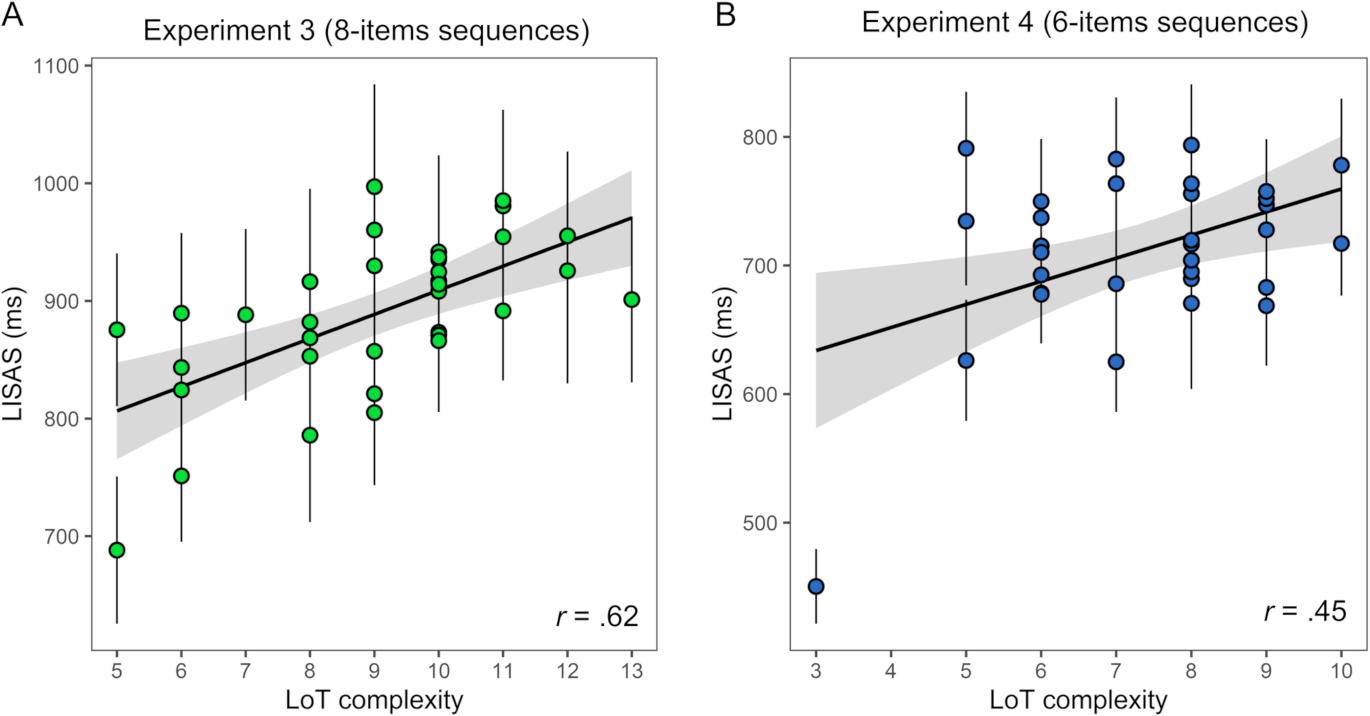
\includegraphics[scale=1]{journal.pcbi.1008598.g006.PNG}
   \centering
   %Linear relationship between LoT complexity and violation detection task performance (LISAS) in: (A) experiment 3 (8-items sequences) and (B) experiment 4 (6-items sequences).
   \caption{Relación lineal entre la complejidad LoT y el desempeño de la tarea de detección de violaciones (LISAS) en: (A) Experimento 3 (secuencias de 8 elementos) y (B) Experimento 4 (secuencias de 6 elementos)}
   \label{PlosBIO-F6}
\end{figure}
\sergio{la figura no está traducida}

\subsection{Experimento 5: secuencias auditivas y visuales}

%The observation of a LoT complexity effect on sequences of length 8 and higher is consistent with our initial claim that individuals spontaneously apply simple rules (mainly based on nested repetitions) in order to recode auditory sequences in a compressed abstract form in memory. It may be argued, however, that rather than being abstract and universal, some of these effects may reflect the great ability of our auditory system to manipulate and find regularities in acoustic stimuli (90); whether it is in spoken language or in music listening. In experiment 5, we wished to replicate the findings of previous experiment and extend them to the visual modality. Although we expected a reduced performance, given that audition is generally superior to vision in the processing of temporal information (91), we still predicted a correlation of performance with our complexity metric, since our language was originally designed for a visual paradigm (58) and relies on abstract mental operations rather than on specific acoustic coding mechanisms. Twelve sequences of 8 items (see Fig. S7), allowing to use a sufficient number of trials while still expecting clear complexity effects, were presented to a group of participants in both a visual and in an auditory form (in different experimental blocks), using the same violation detection paradigm. Due to constraints in the perception of repeated visual stimuli, stimulus onset asynchrony was lengthened to 400 ms in both auditory and visual sessions, resulting in a sequence duration of 3000 ms (compared to 1800 ms in experiment 2).

La observación de un efecto de la complejidad LoT en secuencias de longitud 8 y superior es consistente con nuestro planteo inicial de que los individuos espontáneamente aplican reglas simples (basada principalmente en repeticiones anidados) con el fin de recodificar secuencias auditivas en una forma abstracta más comprimido en la memoria. Sin embargo, se puede argumentar que -en lugar de ser abstractos y universales- algunos de estos efectos pueden reflejar la gran capacidad de nuestro sistema auditivo para manipular y encontrar regularidades en los estímulos acústicos (\cite{f90}); ya sea en el lenguaje hablado o escuchando música. En el experimento 5, deseamos replicar los hallazgos del experimento anterior y extenderlos a una modalidad visual. A pesar de que esperábamos un rendimiento reducido (dado que la audición es generalmente superior a la visión en el procesamiento de información temporal (\cite{f91})) todavía esperamos encontrar una correlación del rendimiento con nuestra métrica de complejidad, ya que nuestro lenguaje fue diseñado originalmente para un paradigma visual (\cite{amalric2017language}) y se basa en operaciones mentales abstractas más que en mecanismos de codificación acústica específicos. Se presentaron a un grupo de participantes doce secuencias de 8 elementos (ver Figura~\ref{PlosBIO-F7}) tanto en forma visual como auditiva (en diferentes bloques experimentales), utilizando el mismo paradigma de detección de violaciones. Debido a las limitaciones en la percepción de estímulos visuales repetidos, la asincronía inicio de estímulo se alargó a 400ms en ambas sesiones (auditivas y visuales), lo que resulta en una duración de la secuencia de 3000ms (en comparación con 1800ms en el experimento 2).

\subsubsection*{Efectos de complejidad y modalidad}

%To assess the impact of LoT complexity and modality on performance, we first estimated a mixed model including complexity and modality as fixed factors and participants as a random factor. Effects of LoT complexity (t(486.0) = 3.08, p = .003), modality (average LISAS of 1110 ms in visual blocks vs. 780 ms in auditory blocks; t(486.0) = 14.1, p < .0001) and their interaction (t(486.0) = 3.19, p = .002) were significant. The slope of the complexity effect was steeper in the visual than in the auditory modality (+54 ms vs. +22 ms, t(486) = 3.19; see Figure 7, and Fig. S8). Separate analyses indicated that LoT complexity was a strong predictor of performance for visual sequences (t(233.0) = 6.82, p < .0001; r = .76), and also for auditory sequences (t(237.0) = 3.76, p < .001; r = .63).

Para evaluar el impacto de la complejidad y la modalidad de LoT en el rendimiento, primero estimamos un modelo mixto que incluye la complejidad y la modalidad como factores fijos y los participantes como un factor aleatorio. Efectos de la complejidad de LoT (t (486.0) = 3.08, p = .003), modalidad (LISAS promedio de 1110 ms en bloques visuales vs 780 ms en bloques auditivos; t (486.0) = 14.1, p < .0001) y su interacción (t (486.0) = 3.19, p< = 0,002) fueron significativas. La pendiente del efecto de complejidad fue más pronunciada en la modalidad visual que en la auditiva (+5 4 ms frente a +22 ms, t (486) = 3,19; ver Figura 7 y Figura S8). Análisis separados indicaron que Lot complejidad era un fuerte predictor de rendimiento para secuencias visuales (t (233. 0) = 6,82, p <0,0001; r. = 76), y también para las secuencias auditivas (t (237,0) = 3,76, p < . 001; r = .63).

%Note that, although the effects appeared stronger in the visual modality, the average performance in the visual and the auditory modality were highly correlated (r = .85, p < .0001). This suggests a common, cross-modal mechanism underlying the observed differences in performance between sequences. It can however be acknowledged, here again, that differences in performance across sequences are not entirely explained by complexity: residuals of linear regressions with LoT complexity in the visual and in the auditory modality (using average LISAS per sequence) were correlated (r = .73, t(13) = 3.92; p = .002).

Nótese que, aunque los efectos parecían más fuertes en la modalidad visual, el desempeño promedio en la modalidad visual y auditiva estuvieron altamente correlacionados ($r = .85, p < .0001$). Esto sugiere un mecanismo común entre las modalidades subyacente a las diferencias observadas en el rendimiento entre secuencias. Sin embargo, se puede reconocer nuevamente que las diferencias en el rendimiento entre secuencias no se explican completamente por la complejidad: los residuos de regresiones lineales con la complejidad LoT en la modalidad visual y en la modalidad auditiva (usando LISAS promedio por secuencia) estuvieron correlacionados ($r = .73, t (13) = 3.92; p = .002$).

%The number of false alarms per sequence was related to the task modality (mean number of FA: 0.58 in auditory blocks; 1.16 in visual blocks; difference between modalities: t(487.0) = 5.73, p < .0001) but not to sequence LoT complexity (t(487.0) = 0.08, p = .935).

El número de falsas alarmas por secuencia se relacionó con la modalidad de la tarea (número medio de FA : 0.58 en bloques auditivos; 1.16 en bloques visuales; diferencia entre modalidades: $t (487.0) = 5.73, p <0.0001$) pero no con la complejidad LoT ($t(487.0) = 0.08, p = .935$).

\begin{figure}[t!]
   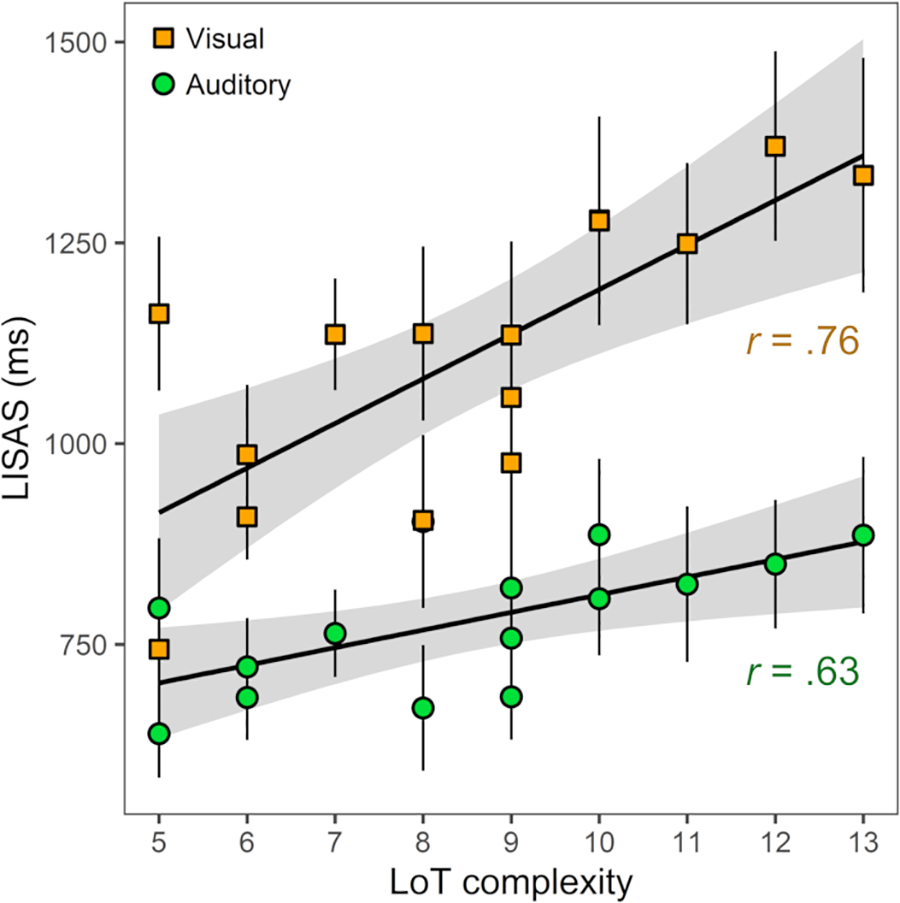
\includegraphics[scale=1]{journal.pcbi.1008598.g007.PNG}
   \centering
   % Linear relationship between LoT complexity and violation detection task performance (LISAS) for each modality in experiment 5 (8-items auditory and visual sequences).
   \caption{Relación lineal entre complejidad LoT y rendimiento en tareas de detección de violación (LISAS) para cada modalidad en experimento 5 (secuencias auditivas y visuales de 8 elementos)}
   \label{PlosBIO-F7}
\end{figure}
\sergio{la figura no está traducida}

\subsubsection*{Efectos de sorpresa}

%As in previous experiments, a surprise effect was also observed in both modalities when considered independently: deviants inducing rare transitions were more easily and quickly detected than frequent ones (effect of surprise in a mixed model with auditory trials only: t(237.0) = 3.87, p < .001; r = –.65; with visual trials only: t(233.0) = 6.79, p < .0001; r = –.78). This effect suggests that a common, or at least similar, mechanism is at play in the encoding of statistical regularities characterizing the sequences in both the visual and the auditory modality. 

Como en los experimentos anteriores, también se observó un efecto sorpresa en ambas modalidades cuando se consideraron de forma independiente: las súper-desviaciones que inducían transiciones raras se detectaban más fácil y rápidamente que las relacionadas a elementos frecuentes (efecto de sorpresa en un modelo mixto con pruebas auditivas solamente: $t(237.0) = 3.87, p < .001; r =-.65$; solo con pruebas visuales: $t (233.0) = 6.79, p < .0001; r = –.78$). Este efecto sugiere que un mecanismo común, o al menos similar, está en juego en la codificación de regularidades estadísticas que caracterizan las secuencias tanto en la modalidad visual como en la auditiva.

%In order to test whether evidence for sequence compression could still be observed after the surprise effect was taken into account, we performed a comparison of mixed effects models. The null model included the surprise predictor, the modality as a categorical predictor and subject identity as random factor. It was compared against a full model including the same predictors, with addition of the LoT complexity. This comparison was highly significant (χ²(1) = 19.0, p < .0001), indicating that goodness of fit improved when LoT complexity was added to the model. All three fixed effects were significant in the full model (LoT complexity: t(486.0) = 4.39, p < .0001; surprise: t(486.0) = 4.54, p < .0001; modality: t(486.0) = 14.2, p < .0001, see Table 1).

Para probar si aún se podía observar evidencia de compresión de secuencia después de que se tuvo en cuenta el efecto sorpresa, realizamos una comparación de modelos de efectos mixtos. El modelo nulo incluyó el predictor de la sorpresa, la modalidad como predictor de categoría y la identidad del sujeto como factor aleatorio. Se comparó con un modelo completo que incluía los mismos predictores, con la adición de la complejidad LoT. Esta comparación fue altamente significativa ($\chi^2 (1) = 19.0, p < .0001$), lo que indica que el ajuste mejoró cuando se agregó la complejidad LoT al modelo. Los tres efectos fijos fueron significativos en el modelo completo (complejidad LoT: $t (486.0) = 4.39, p < .0001$; sorpresa: $t (486.0) = 4.54, p < .0001$; modalidad: $t (486.0) = 14.2, p <0,0001$, ver Tabla~\ref{PlosBIO-T1}).

%Overall, the results obtained in the visual modality are very similar to those obtained in the auditory modality in the same and in previous experiments. We however observed here stronger effects of both LoT complexity and surprise. It should be noted that the overall difficulty of the task increased in the visual modality (as indicated by higher average miss rates per sequence; 22\% vs. 11\%, t(14) = 7.49, p < .0001; and longer average response times per sequence; 831 ms vs. 645 ms, t(14) = 10.5, p < .0001). 8-items visual sequences may have been more difficult to encode than 8-items auditory sequences, due to the known superiority of the auditory processing system in the processing of temporal sequences and rhythms (90,92). This increased encoding difficulty in the visual domain may have in turn lead to an increased need for the “mental sequence compression” mechanism that our language of thought aims to describe.

En general, los resultados obtenidos en la modalidad visual son muy similares a los obtenidos en la modalidad auditiva en el mismo experimento y en los anteriores. Sin embargo, observamos aquí efectos más fuertes tanto de la complejidad LoT como de la sorpresa. Hay que señalar que la dificultad general de la tarea aumenta en la modalidad visual (como se indica por el aumento promedio de las tasas de error por secuencia; 22\% vs. 11 \%, $t (14) = 7.49, p <0.0001$; y del tiempo medio de respuesta por secuencia; 831ms frente a 645ms, $t(14) = 10.5, p <0.0001$). En las secuencias visuales de 8 elementos pueden haber sido más difíciles de codificar que las secuencias auditivas de 8 elementos, debido a la superioridad conocida del sistema auditivo para el procesamiento de secuencias temporales y ritmos~\cite{f90,f92}. Esta mayor dificultad de codificación en el dominio visual puede, a su vez, llevar a una mayor necesidad de utilizar el mecanismo de ``compresión de la secuencia mental'' que nuestro LoT pretende describir.

%The present experiment also extends the results of experiment 3 by using a slower presentation rate. Indeed, although the participants in experiment 5 appeared to respond faster (in the auditory blocks) than those from experiment 3, the same relationship with complexity was found (correlation of performance with LoT complexity of.62 and.63 respectively). It suggests that the effect of complexity is robust across sequence durations (as expected given than LoT complexity is based on abstract sequence patterns). More importantly, the fact that a similar complexity effect was observed irrespective of the modality is consistent with the idea of “language of thought” used to compress sequential information at an abstract, symbolic level. Such an assumption has already been supported by results from Yildirim and Jacobs (93), who showed cross-modal transfer of sequence knowledge: learning to categorize visual sequences facilitated the categorization of auditory sequences and vice versa. In fact, the language we used here was initially designed to represent visually presented, geometrical patterns (58). The present results thus confirm that the present language of thought can account for sequence representations in various modalities, presentation contexts and sequence lengths.

El presente experimento extiende también los resultados del experimento 3 utilizando una tasa de presentación más lenta. De hecho, aunque los participantes del experimento 5 parecían responder más rápido (en los bloques auditivas) que los del experimento 3, se encontró la misma relación con la complejidad LoT (correlación de rendimiento con complejidad LoT de 0,62 y 0,63, respectivamente). Esto sugiere que el efecto de la complejidad es robusto a través de la duración de las secuencias (como se esperaba dado que la complejidad LoT se basa en patrones de secuencias abstractos). Más importante aún, el hecho de que se observó un efecto de complejidad similar independientemente de la modalidad es consistente con la idea de un ``lenguaje de pensamiento'' (LoT) utilizado para comprimir información secuencial a un nivel simbólico abstracto. Tal suposición se apoya también en los resultados de Yildirim y Jacobs~\cite{yildirim2015learning}, que mostraron efectos de transferencia de aprendizaje entre modalidades de las secuencias: aprender a categorizar secuencias visuales facilitó la categorización de secuencias auditivas y viceversa. De hecho, el lenguaje que usamos aquí fue inicialmente diseñado para representar patrones geométricos presentados de manera visual~\cite{amalric2017language}. Los presentes resultados confirman así que el lenguaje actual del pensamiento puede dar cuenta de las representaciones de secuencia en diversas modalidades, contextos de presentación y longitudes de secuencias.

\subsection{Análisis adicional: comparación con otras medidas de complejidad de secuencias}

%The complexity, or “compressibility”, of a sequence can be assessed in several ways, and various measures have been previously proposed in the psychological literature (e.g. 17,30,34,41,44,95–98). In this last section, we examined how our LoT complexity value compares to six other measures, which we list below, in predicting task performance over different sequence lengths.

La complejidad, o la ``compresibilidad'', de una secuencia se puede evaluar de varias formas, y varias medidas se han propuesto incluso previamente en la literatura psicológica~\cite{f17,f30,f34,f41,f44,f95,f96,f97,f98}. En esta sección, examinamos cómo nuestro valor de complejidad LoT se compara con otras seis medidas para predecir el desempeño de la tarea en diferentes secuencias longitudes. Estas medidas fueron las siguientes:

%Chunk complexity: following the observation that the number of chunks (or runs) is correlated to performance in sequence encoding tasks (e.g. 34), we here define chunk complexity using the formula proposed by Mathy & Feldman (16), which they showed to correlate with performance in the encoding of series of digits:, where K is the number of chunks and Li the length of the i-th run. Note that contrary to Mathy & Feldman (16), whose sequences where composed of digits and chunks defined based on constant (positive or negative) increments from one digit to the next (e.g. “1234”, “7531”), we here simply define chunks as consecutive repetitions of the same item, e.g. the sequence “AAABAA” has a 3 chunks, and a chunk complexity of log2(4) + log2(2) + log2(3).

\paragraph{Complejidad de fragmentos}: Siguiendo la observación que el número de fragmentos (o trazas) se correlaciona con el desempeño en tareas de codificación de secuencias~\cite{f34}, definimos la complejidad de fragmentos utilizando la fórmula propuesta por Mathy \& Feldman~\cite{f34}, la cual mostraron se correlaciona con el rendimiento en la codificación de series de dígitos. 

$$ \text{complejidad de fragmentos} = \sum_{i = 1}^{K} \log_2(1+L_i) $$ donde $K$ es el número de fragmentos y $L_i$ la longitud de la i-ésima traza. Se debe tener en cuenta que -- al contrario que en~\cite{f34} cuyas secuencias estaban compuestas de dígitos y los fragmentos definidos en incrementos constantes (positivos o negativos) de un dígito respecto del siguiente (por ejemplo, ``1234'', ``7531'' son ambos un sólo fragmento o traza) -- aquí simplemente definimos los fragmentos como repeticiones consecutivas del mismo elemento. Por ejemplo, la secuencia ``AAABAA'' tiene 3 fragmentos, y una complejidad de fragmentos = $\log_2(4) + \log_2(2) + \log_2(3)$.

%Entropy is a measure of information that quantifies the uncertainty of a distribution. Here, we compute the Shannon entropy of the probability of pairs of items, (AA, AB, BA, BB), in order to capture the effect of order-1 transition probabilities (85). Given that the probability of a given pair is defined as, H is computed as follow:
%H = ...
%We used the convention that 0 × log2(0) = 0 when null probabilities occurred.

\paragraph{Entropía (H)}: Es una medida de información que cuantifica la incertidumbre de una distribución. Aquí calculamos la entropía de Shannon para la probabilidad de pares de elementos (AA, AB, BA, BB), para capturar el efecto de las probabilidades de transición de un paso~\cite{f85}. Dado que la probabilidad de un terminado par se define como $P(X,Y) = P(X) P(Y \mid X)$, H se calcula de la siguiente manera:

\begin{align*}
H = - [ 
     P(A) P(A \mid A) (\log_2 P(A) + \log_2 P(A\mid A)) \\
    +P(A) P(B \mid A) (\log_2 P(A) + \log_2 P(B\mid A)) \\
    +P(B) P(A \mid B) (\log_2 P(B) + \log_2 P(A\mid B)) \\
    +P(B) P(B \mid B) (\log_2 P(B) + \log_2 P(B\mid B)) 
     ] 
\end{align*}
usamos la convención que $0 * \log_2(0) = 0$ cuando la probabilidad es nula.

%Lempel-Ziv complexity is derived from the popular lossless data compression algorithm, the Lempel-Ziv (LZ) algorithm (98). Briefly, the LZ algorithm works by scanning the sequence from left to right and adding to a vocabulary each new substring it has never encountered before. LZ complexity is the number of substrings in this vocabulary once the scan is complete. Beyond the field of computer data compression, LZ complexity has been used in various domains, for instance, to measure the complexity of rhythmic patterns in music (61), to account for the complexity of human (99) and mouse behaviors (100), to explain the existence of universal properties within all natural languages (101), or to measure the complexity of input-output mappings found in various domains of science and engineering (102,103). 

%The number of subsymmetries is the number of symmetric sub-sequences of any length within a sequence. For instance, the sequence AABBAB has two symmetric sub-sequences of length 2 (AA and BB), one of length 3 (BAB), and one of length 4 (ABBA), for a total of four subsymmetries. This measure was proposed by Alexander and Carey (94) and shown to be negatively correlated to performance in perception and production tasks with visual and auditory patterns (94,104). 

\paragraph{Complejidad Lempel-Ziv}: Se deriva del popular algoritmo de compresión de datos de Lempel-Ziv (LZ)\cite{f98}. Brevemente, el algoritmo LZ funciona escaneando la secuencia de izquierda a derecha y agregando a un vocabulario cada nueva subcadena que no había encontrado hasta entonces. La complejidad de LZ es el número de subcadenas en este vocabulario una vez que se completa el escaneo. Más allá de su aplicación a la compresión de datos informáticos, La complejidad LZ se ha utilizado en varios dominios, por ejemplo, para medir la complejidad de patrones rítmicos en la música~\cite{f61}, para evaluar la complejidad de comportamientos humanos~\cite{f99} y de ratones~\cite{f100}, para explicar la existencia de propiedades universales entre los lenguajes naturales~\cite{f101}, o para medir la complejidad de distintas asignaciones de entrada-salida que se encuentran en varios dominios de la ciencia y la ingeniería~\cite{f102,f103}.

%The number of subsymmetries is the number of symmetric sub-sequences of any length within a sequence. For instance, the sequence AABBAB has two symmetric sub-sequences of length 2 (AA and BB), one of length 3 (BAB), and one of length 4 (ABBA), for a total of four subsymmetries. This measure was proposed by Alexander and Carey (94) and shown to be negatively correlated to performance in perception and production tasks with visual and auditory patterns (94,104). 

\paragraph{Subsimetrías}: El número de subsimetrías es el número de subsecuencias simétricas de cualquier longitud dentro de una secuencia. Por ejemplo, la secuencia ``AABBAB'' tiene dos subsecuencias simétricas de longitud 2 (``AA'' y ``BB''), una de longitud 3 (``BAB'') y una de longitud 4(``ABBA''), lo que arroja un total de cuatro subsimetrías. Esta medida fue propuesta en~\cite{f94} y se mostró que estaba correlacionada negativamente con el desempeño en percepción y tareas de producción con patrones visuales y auditivos~\cite{f94,f104}.

%Change complexity is an measure proposed by Aksentijevic and Gibson (47), based on the notion of “change” (the inverse of invariance), computed across all sub-sequences contained in a sequence, and showing interesting properties such as a sensibility to periodicity and symmetries.

\paragraph{Complejidad del cambio}\cite{f47}: Es una medida basada en la noción de ``cambio'' (la inversa de la invariancia), calculada 
a través de todas las subsecuencias contenidas en la secuencia y que muestra propiedades interesantes como sensibilidad a la periodicidad y a las simetrías.

%Algorithmic complexity was introduced by Gauvrit et al. (44,45) and Soler-Toscano et al. (46). It is based on the mathematical definition of Kolmogorov-Chaitin complexity (39,40) and derived from the probability of obtaining a given pattern in the output of a randomly chosen universal Turing machine that halts.

\paragraph{Complejidad algorítmica D(5)}: Una medida computable propuesta en~\cite{f44,f45,f46} para cadenas cortas que busca aproximar la complejidad de Kolmogorov, derivada de la probabilidad de obtener un patrón dado en la salida de una máquina de Turing universal que se detiene y elegida al azar.

%LoT chunk complexity. Note that the alternative measures of complexity tested here, which provide a unique metric for each pattern, are conceptually quite different from the one we propose. LoT complexity is based on the proposal that humans possess a language of thought, composed of a small number of atomic rules which they use recursively to recode the abstract structure of the pattern in a compressed form. Such a recursive representation differs radically from, say, the mere counting of the number of chunks. However, it is possible to combine the two ideas. The formal language we proposed produces many legal expressions for each sequence (the number of possible expressions can reach several tens of thousands for a sequence of length 16), which correspond to distinct “parses” of the same sequence. We initially assumed that the shortest expression is always selected (with the limitation that two or more expressions can have the same “shortest” length for some sequences), and thus that LoT complexity is equal to the shortest possible description using this language. However, it is unclear whether humans could ever search such a vast space of possibilities. A more plausible hypothesis is that participants begin by chunking the sequence into groups of identical items, and only then compress it by detecting repetitions of those chunks (for a similar proposal, see 33,49). According to this idea, the shortest sequence should only be accepted when its proposed parsing coincides with chunk boundaries. Consider the sequence ABBAAB, which consists of 4 chunks [A] [BB] [AA] [B]. According to our language, its optimal description is [AB] [BA] [AB] (i.e. 3 repetitions of the stay-change program; LoT complexity = 5), but that representation does not coincide with chunk boundaries. Interestingly, the data suggested that the shortest description may not be the best in similar cases (see Experiment 2, Results and discussion). To test this idea, we recomputed LoT values restricted to chunk-preserving expressions (i.e. excluding expressions producing “A][A” or “B][B”). We called this new LoT complexity the LoT chunk complexity. Its value was higher than the original one for 58% of sequences (and remained the same for the others). For instance, the sequence “ABBAAB” from the previous example, when described as four chunks [A] [BB] [AA] [B], has an LoT-chunk complexity = 9. We tested LoT chunk complexity as another potential predictor of behavioral performance.

\paragraph{Complejidad LoT de fragmentos}: Tenga en cuenta que las medidas alternativas de complejidad probadas aquí, que proporcionan una métrica única para cada patrón, son conceptualmente diferentes de las propuestas en la complejidad LoT. La complejidad LoT se basa en la propuesta de que los humanos poseen un lenguaje del pensamiento, compuesto por un pequeño número de reglas atómicas que utilizan recursivamente para recodificar la estructura abstracta del patrón en forma comprimida. Esa representación recursiva difiere radicalmente de, digamos, el mero recuento del número de trazas. Sin embargo, es posible combinar las dos ideas. El lenguaje formal que propusimos produce muchas expresiones legales para cada secuencia (el número de expresiones posibles puede alcanzar varias decenas de miles para una secuencia de longitud 16), que corresponden a distintos análisis sintácticos (\textit{parseos}) de la misma secuencia. Inicialmente asumimos que la expresión más corta es siempre seleccionada, y por lo tanto, la complejidad de LoT es igual a la descripción más corta posible utilizando este lenguaje. Sin embargo, no está claro si los humanos podrían alguna vez buscar en un espacio tan vasto de posibilidades. Una hipótesis más plausible es que los participantes comienzan dividiendo las secuencias en grupos de elementos idénticos, y sólo luego comprimirlo detectando repeticiones de esas trozas (para una propuesta similar, vease~\cite{f33,f49}). De acuerdo con esta idea, la secuencia más corta sólo debe aceptarse cuando el análisis sintáctico coincida con los límites de las trazas. Considere la secuencia ``ABBAAB'', que consta de 4 trozas [A] [BB] [AA] [B]. Según nuestro lenguaje, su descripción óptima es [AB] [BA] [AB] (es decir, 3 repeticiones del programa de mantener posición y cambiar; complejidad LoT = 5), pero esa representación no coincide con los límites de los fragmentos. Curiosamente, los datos sugieren que la descripción más corta puede no ser la óptima en casos similares (ver~\ref{ploscompresults-exp2}). Para probar esta idea, volvimos a calcular los valores de LoT restringiendo los programas a expresiones que preserven los fragmentos (es decir, excluyendo expresiones que produzcan ``A] [A'' o ``B] [B''). Llamamos a esta nueva complejidad de LoT la complejidad LoT de fragmentos. Su valor fue mayor que el original para el 58\% de las secuencias (y permaneció igual para las demás). Por ejemplo, la secuencia ``ABBAAB'' del ejemplo anterior, cuando es escrita como cuatro fragmentos [A] [BB] [AA] [B], tiene una complejidad LoT de fragmentos = 9. Probamos la complejidad LoT de fragmentos como otro predictor potencial del desempeño conductual.

 \subsection{Comparación de modelos}
 %FALTA TRADUCIR DESDE ACA. LAS CITAS ESTAN TODAS YA PASADAS. FIGURAS Y TABLAS TAMBIEN. FALTA LA INFORMACION SUPLEMENTARIA NOMAS
 
 %With the aim of arbitrating between previous models, we pooled data from all previous experiment with auditory sequences (using LISAS to index task performance), excluding súper-deviants. Unfortunately, due to the nature of algorithmic complexity (derived from the output frequency for a pattern using small Turing machines, which decreases rapidly with sequence length), no values were available for the ten length-16 patterns that we used in experiment 1, as well as for one length-12 pattern used in experiment 2. Those sequences were therefore excluded from some analyses. The sequence AAAAAA from experiment 4 was also excluded. Consequently, a first pooled dataset, for which all 8 different predictors could be compared, included performance with 77 different auditory sequences (and 88 different participants), of length 6 (N = 31 sequences), length 8 (N = 35) and length 12 (N = 11), while a second one, for which 7 different predictors were compared, also included sequences of length 16 (N = 88 sequences, 113 participants). 
 
 Para realizar los análisis, se combinaron los datos de todos los experimentos anteriores con las secuencias auditivas (usando LISAS para indexar el desempeño de la tarea) y excluyendo las súper-desviaciones. Desafortunademente, debido al procedimiento utilizado para calcular la complejidad algorítmica D(5), no había valores disponibles para los diez patrones de longitud 16 que usamos en el experimento 1, así como para un patrón de longitud 12 utilizado en el experimento 2. Esas secuencias fueron, por lo tanto, excluidas de algunos análisis. La secuencia ``AAAAAA'' del experimento 4 fue también excluida. En consecuencia, se presenta un primer conjunto de datos para el cual las 8 medidas pueden compararse, que incluye el rendimiento de las 77 secuencias auditivas diferentes (y 88 participantes diferentes), de longitud 6 (n = 31 secuencias), longitud 8 (n = 35) y longitud 12 (n= 11). Y un segundo conjunto para el que se compararon 7 medidas diferentes, que incluye también las secuencias de longitud 16 (n = 88 secuencias, 113 participantes).
 
 %To assess whether one measure was a better predictor of task performance, we first computed different mixed models, which all included the predictor of interest as the only fixed effect and participants as a random effect (note that this is a way to control for the fact that different participants coming from different experiments, with different sets of stimuli, were pooled together). We then report the Akaike information criterion (AIC) as an indicator of goodness of fit which penalizes for model complexity (i.e. the number of predictors); the model with the lowest AIC value being considered the best (or with lowest Δ(AIC) value, i.e. the relative difference in AIC with the best model: for a model i, Δ(AIC)i = AICi — AICmin). Note that we also report the Bayesian information criterion (BIC) which, in addition, scales the strength of penalization by the (log) number of data points (105). Second, since, as we reported earlier, surprise derived from the learning of transition probabilities may strongly affect the performance in such violation detection task, all these models were estimated again, this time including surprise as a fixed effect covariate.

Para evaluar si alguna de las medidas es un mejor predictor del desempeño de la tarea, primero calculamos diferentes modelos mixtos, los cuales todos incluyeron el predictor de interés como el único efecto fijo y a los participantes como un efecto aleatorio (tenga en cuenta que esta es una forma de controlar el hecho de que diferentes participantes, provenientes de diferentes experimentos, con diferentes conjuntos de estímulos, se agruparon). Luego informamos el criterio de información de Akaike (AIC) como un indicador de ajuste del modelo que penaliza la complejidad (es decir, el número de predictores). El modelo con el valor de AIC más bajo se considera el mejor (o con el valor ``$\Delta$ (AIC)'' más bajo, es decir, la diferencia relativa en AIC con el mejor modelo: para un modelo $i$, $\Delta (AIC) i = AIC_i - AIC_{min})$. Tenga en cuenta que también informamos el criterio de información bayesiano (BIC) que, además, escala la fuerza de la penalización por el número (en escala logarítmica) de puntos de datos~\cite{f105}. En segundo lugar, dado que hemos informado previamente que la sorpresa derivada del aprendizaje de las transiciones de probabilidad puede afectar fuertemente el desempeño en la tarea de detección de violaciones, todos estos modelos fueron computados nuevamente incluyendo la sorpresa como un efecto fijo covariable.

\subsection{Datos para secuencias de longitud 6, 8 y 12}

%Sixteen different mixed models were fitted using datasets with sequences of length 6, 8 and 12. As illustrated in Figure 8A, model fit, as indexed by the Δ(AIC) value, always improved when the surprise associated to the deviants was included in the model. This finding confirms that the effect due to transition probabilities needs to be taken into account when assessing responses to deviants in the violation detection paradigm. The improvement in model fit was smallest for the model with entropy. This effect was expected since entropy and surprise are two tightly related information measures (Shannon entropy is the average of Shannon surprise).

Se ajustaron dieciséis modelos mixtos diferentes utilizando el conjunto de datos con secuencias de longitud 6, 8 y 12. Como se ilustra en la Figura~\ref{PlosBIO-F8}A, el ajuste de los modelos indexados por el valor $\Delta$ (AIC), siempre mejoraron cuando se incluía en el modelo la sorpresa asociada a las desviaciones. Este hallazgo confirma que el efecto asociado a las transiciones de probabilidad debe tomarse en cuenta al evaluar las respuestas a desviaciones en el paradigma de detección de violaciones. La mejora en el ajuste del modelo fue mínima para el modelo con entropía. Este efecto fue esperado ya que la entropía y la sorpresa son dos medidas de información estrechamente relacionadas (es decir, la entropía de Shannon es el promedio de la sorpresa de Shannon).

%When considering either only single-predictor models (i.e. without the surprise covariate) or two-predictors models (i.e. with surprise), the two best models were the ones with our modified version of LoT complexity (i.e. LoT-chunk, with the “no-splitting” chunks constraint) followed by the one with original LoT complexity (see Table 2). In order to test whether the differences in the raw AIC values were relevant, we computed the Akaike weights for this set of 14 models. Akaike weights can be interpreted as the probability that a given model is the best model of the set (106). Akaike weight was.99 for the LoT-chunk complexity (+ surprise) model,.01 for the LoT complexity (+ surprise) model, and below.01 for all other models (see Table 2 and Figure 8A).

Al considerar sólo los modelos de predictor único (es decir, sin la covariable sorpresa) o modelos de dos predictores (es decir, con sorpresa), los dos mejores modelos eran los que tenían nuestra versión modificada de la complejidad LoT (es decir, la complejidad LoT de fragmentos) seguido por el que tenía la complejidad de LoT original (ver Tabla~\ref{PlosBIO-T2}). Para probar si las diferencias en los valores de AIC eran significativas, calculamos los pesos Akaike para este conjunto de 14 modelos. Los pesos de Akaike se pueden interpretar como la probabilidad de que un modelo dado es el mejor modelo del conjunto~\cite{f106}. El peso de Akaike fue $.99$ para el modelo de complejidad LoT de Fragmentos (+ sorpresa), $.01$ para la complejidad LoT (+sorpresa) y por debajo de $.01$ para todos los demás modelos (consultar la Tabla~\ref{PlosBIO-T2} y la Figura~\ref{PlosBIO-F8}A).

\begin{figure}[t!]
   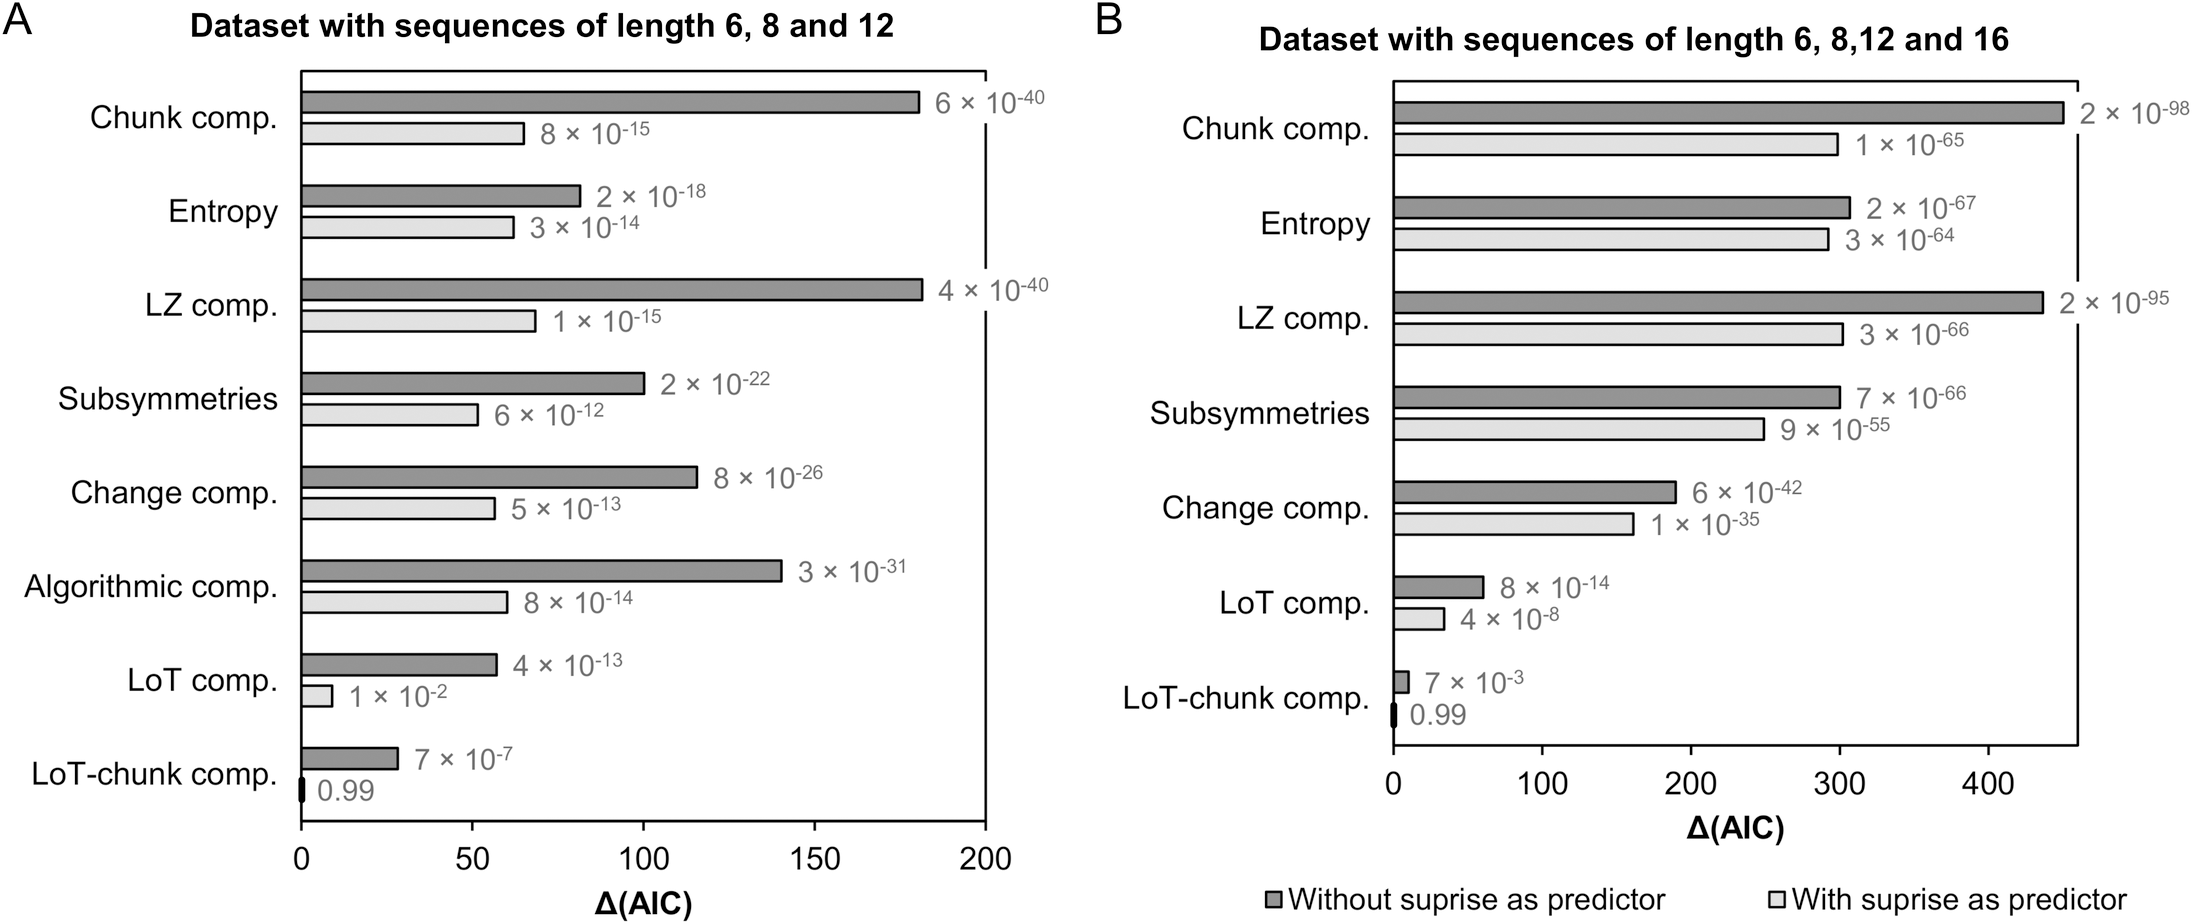
\includegraphics[scale=0.8]{figuras/plosbio/journal.pcbi.1008598.g008.PNG}
   
   \centering
   %%Figure 8: Δ(AIC) for the sixteen mixed models tested using the dataset including the task performance (LISAS) for sequences of length 6, 8 and 12 (A), and for the twelve different mixed models tested using the dataset with sequences of length 6, 8, 12 and 16 (B). The fixed effect of interest is indicated along the vertical axis (all models included participants as a random effect and could include surprise as a covariate — light gray bars). Akaike weight for each model is also reported. The model with lower AIC (Δ(AIC) = 0) is indicated by short dark vertical line on the vertical axis.
   
   \caption{$\Delta$ (AIC) para los dieciséis modelos mixtos probados utilizando el conjunto de datos que incluye el desempeño de la tarea (LISAS) para secuencias de longitud 6, 8 y 12 (A), y para los doce modelos mixtos diferentes probados utilizando el conjunto de datos de longitud 6, 8, 12 y 16 (B). El efecto fijo de interés se indica a lo largo del eje vertical (todos los modelos incluyen a los participantes como efecto aleatorio y pueden incluir la sorpresa como una covariable (barras de color gris claro). Se informa también el peso Akaike para cada modelo. El modelo con AIC más bajo ($\Delta$ (AIC) = 0) se indica con una línea vertical corta y oscura en el eje vertical}
   \label{PlosBIO-F8}
\end{figure}
\sergio{la figura no está traducida}

%Although correlations between performance and LoT complexity in experiments 2, 3 and 4 (lengths 6, 8 and 12) were small compared to experiment 1 (length 16), LoT complexity again appears as the best predictor of performance in the violation detection task with sequences of length ≤ 12. Notably, the constraint of excluding, for each pattern, the expressions that resulted in the splitting of a chunk (before the selection of shortest expression) improved the fit of behavioral data. This observation suggests that participants did not always find the best way of coding some patterns (best in the sense of the language of thought considered here) because of a propensity to perform an initial chunking solely based on consecutive runs of identical items. 

Aunque las correlaciones entre el rendimiento y la complejidad LoT en los experimentos 2, 3 y 4 (longitudes 6, 8 y 12) eran pequeñas en comparación con el experimento 1 (longitud 16), la complejidad LoT vuelve a aparecer como el mejor predictor del rendimiento en la detección de infracciones para secuencias de longitud $\leq$ 12. En particular, la complejidad LoT de fragmentos y su restricción de excluir para cada patrón las expresiones que resultan en la división de un fragmento (antes de la selección de la expresión más corta) mejoró el ajuste a los datos de comportamiento. Esta observación sugiere que los participantes no siempre encontraron la mejor manera de codificar algunos patrones (mejor en el sentido del lenguaje de pensamiento considerado aquí) debido a una propensión a realizar una fragmentación basada únicamente en ejecuciones consecutivas de elementos idénticos.

%The next best model was the one with the “number of subsymmetries” predictor (and including the surprise covariate), suggesting that it also provides a good measure of the psychological complexity of patterns. However, while this appeared true here using statistical models partially controlling for sequence length (i.e. by including participant index as a random factor, since each participant performed the task with only one given sequence length), this measure appears inappropriate to predict complexity across different lengths. Indeed, when we computed the Pearson correlation of average LISAS per sequence for the pooled dataset (sequences of length 6, 8 and 12), we obtained a positive correlation value of.39. Such positive correlation is in conflict with the presupposition that patterns containing more symmetries should be simpler. This is explained by the fact that the number of subsymmetries tends to increase with sequence length. These correlations were actually negative when each length was considered independently (r = –.44 for length 6; r = –.54 for length 8; and r = –.58 for length 12). This is illustrated in Figure 9, where the average LISAS for each sequence is presented in relation to each complexity measure (see also Fig. S9 and Fig. S10 for the equivalent with reaction times and miss rates). To summarize, although this measure is quite good in predicting the complexity of sequences for given length, it fails in predicting the variations in complexity across sequence lengths. 

El siguiente mejor modelo fue el que tenía al predictor de número de subsimetrías (incluyendo la covariable sorpresa), lo que sugiere que también proporciona una buena medida de la complejidad psicológica de los patrones. Sin embargo, si bien esto parecía cierto aquí usando modelos estadísticas que controlan parcialmente la longitud de la secuencia (es decir, al incluir el índice de los participantes como factor aleatorio, ya que cada participante realizó la tarea con una sola longitud de la secuencia), esta medida parece inapropiada para predecir la complejidad en diferentes longitudes. De hecho, cuando calculamos la correlación de Pearson de LISAS promedio por secuencia para el conjunto de datos agrupados (secuencias de longitud 6, 8 y 12), obtuvimos un valor positivo de correlación de $.39$. Tal correlación positiva está en conflicto con la presuposición que los patrones que contienen más simetrías deberían ser más simples. Es debido al hecho que el número de subsimetrías tiende a aumentar con la longitud de la secuencia. Estas correlaciones fueron realmente negativas cuando cada longitud se consideró de forma independiente ($r = –.44$ para la longitud 6; $r= –.54$ para la longitud 8; y $r = –.58$ para la longitud 12). Esto se ilustra en la Figura~\ref{PlosBIO-F9}, donde el LISAS promedio para cada secuencia se presenta en relación con cada medida de complejidad (ver también la Figura~\ref{PlosBIO-F6} y Figura~\ref{PlosBIO-F7} para el equivalente con tiempos de reacción y tasas de fallos). Para resumir, aunque esta medida es bastante buena para predecir la complejidad de las secuencias de una longitud dada, no es eficiente para predecir las variaciones en la complejidad debido al largo de la secuencia.

%Another similar limitation applies to algorithmic complexity, where the correlation observed across lengths (r = .79) is mostly explained by the fact that complexity values present excessive discontinuities with length: algorithmic complexity ranges roughly between 14 and 16 for length 6; between 19 and 23 for length 8; and between 31 and 35 for length 12 (see Figure 9). Such a massive increase in complexity with length is not consistent with behavior. Again, LoT complexity provides a better correlation with the present behavioral data across a large range of sequence lengths, because it correctly predicts that, for instance, some 6-items long sequences can be more complex than some 12-items ones (e.g. ABAAAB, LoT complexity = 10, means LISAS = 778 ms; AAAAAABBBBBB, LoT complexity = 6, mean LISAS = 766 ms).

Otra limitación similar se aplica a la complejidad algorítmica D(5), donde la correlación observada en todas las longitudes ($r = .79$) se debe principalmente a que este valor presenta discontinuidades excesivas con la longitud: la complejidad algorítmica D(5) varía aproximadamente entre 14 y 16 para la longitud 6; entre 19 y 23 para la longitud 8; y entre 31 y 35 para la longitud 12 (ver Figura~\ref{PlosBIO-F9}). Semejantes aumentos de complejidad con la longitud no son coherentes con el comportamiento. De nuevo, la complejidad LoT proporciona una mejor correlación con los datos actuales de comportamiento en una gran rango de longitudes de secuencia, porque predice correctamente que, por ejemplo, algunas secuencias de 6 elementos pueden ser más complejas que algunas de 12 elementos (ejemplo, ABAAAB, Complejidad LoT = 10, promedio LISAS = 778 ms; AAAAAABBBBBB, Complejidad LoT = 6, promedio LISAS = 766 ms).

\begin{table}[]
\centering
\resizebox{\textwidth}{!}{\begin{tabular}{lccccccccc}
\hline
\textit{}               & \multicolumn{4}{l}{\textit{\textbf{Datos para secuencias de longitud 6, 8 y 12}}} & \multicolumn{1}{l}{}     & \multicolumn{4}{l}{\textit{\textbf{Datos para secuencias de longitud 6, 8, 12 y 16}}} \\
\textit{Modelo de efectos fijos}   & \textit{Log-lik.}  & \textit{$\Delta$(AIC)}  & \textit{$\Delta$(BIC)}  & \textit{w(AIC)}  & \multicolumn{1}{l}{\textit{}} & \textit{Log-lik.}   & \textit{$\Delta$(AIC)}   & \textit{$\Delta$(BIC)}  & \textit{w(AIC)}  \\ \hline
\textit{Comp. LoT}          & -14886        & 57         & 51        & 4.0 × 10-13    &                & -16653        & 60         & 55         & 7.8 × 10-14    \\
\textit{Comp. LoT + Sorpresa}     & -14861        & 9         & 9         & 1.1 × 10-2    &                & -16639        & 34         & 34         & 4.1 × 10-8     \\
\textit{Comp. Lot Fragm.}       & -14872        & 28         & 23        & 7.4 × 10-7    &                & -16628        & 10         & 4         & 6.8 × 10-3     \\
\textit{Comp. Lot Fragm. + Sorpresa} & -14857        & 0         & 0         & 0.99       &                & -16622        & 0          & 0         & 0.99        \\
\textit{Comp. Fragmentos}       & -14948        & 180        & 175        & 6.4 × 10-40    &                & -16848        & 450         & 445        & 1.6 × 10-98    \\
\textit{Comp. Fragmentos + Sorpresa} & -14889        & 65         & 65        & 7.5 × 10-15    &                & -16771        & 299         & 299        & 1.4 × 10-65    \\
\textit{Entropía}           & -14899        & 81         & 76        & 2.0 × 10-18    &                & -16776        & 307         & 301        & 2.3 × 10-67    \\
\textit{Entropía + Sorpresa}     & -14888        & 62         & 62        & 3.4 × 10-14    &                & -16768        & 292         & 292        & 3.3 × 10-64    \\
\textit{Comp. LZ}           & -14948        & 181        & 176        & 3.9 × 10-40    &                & -16841        & 436         & 431        & 1.6 × 10-95    \\
\textit{Comp. LZ + Sorpresa}     & -14891        & 68         & 68        & 1.4 × 10-15    &                & -16773        & 302         & 302        & 2.6 × 10-66    \\
\textit{Subsimetrías}         & -14908        & 100        & 94        & 1.2 × 10-22    &                & -16773        & 300         & 294        & 8.8 × 10-55    \\
\textit{Subsimetrías + Sorpesa}    & -14883        & 52         & 52        & 6.2 × 10-12    &                & -16746        & 249         & 249        & 1.3 × 10-17    \\
\textit{Comp. de cambio}       & -14916        & 116        & 110        & 7.6 × 10-26    &                & -16718        & 190         & 184        & 6.2 × 10-42    \\
\textit{Comp. de cambio + Sorpresa}  & -14885        & 57         & 57        & 5.3 × 10-13    &                & -16703        & 161         & 161        & 1.0 × 10-35    \\
\textit{Comp. Algorítmica}      & -14928        & 140        & 135        & 3.4 × 10-31    &                & \multicolumn{4}{c}{N.D.}                               \\
\textit{Comp. Algorítmica + Sorpresa} & -14887        & 60         & 60        & 8.4 × 10-14    &                & \multicolumn{4}{c}{N.D.}                               \\ \hline
\end{tabular}}
%Note. All models included participants as a random effect, and either one or two fixed effect(s) (i.e. “+ Surp.”: with additional surprise fixed effect). Log-lik. = log of the maximum likelihood for the model. Δ(AIC) = AIC difference with the model with the lowest AIC value (where AIC is the Akaike Information Criterion). Δ(BIC) = BIC difference with the model with the lowest BIC value (where BIC is the Bayesian Information Criterion). w(AIC) = Akaike weight.

\caption{Todos los modelos incluyeron a los participantes como efecto aleatorio y uno o dos efectos fijos (es decir, "+ Sorpresa" como efecto fijo sorpresa adicional). Log-lik. = logaritmo de la máxima verosimilitud del modelo. $\Delta$ (AIC) = Diferencia AIC del modelo con el valor de AIC más bajo (donde AIC es el criterio de información de Akaike). $\Delta$ (BIC) = Diferencia BIC del modelo con el valor BIC más bajo (donde BIC es el criterio de información bayesiano). w(AIC) = peso Akaike}
\label{PlosBIO-T2}
\end{table}


\subsection{Datos para secuencias de longitud 6, 8 y 12}

%Fourteen different mixed models (with participants as a random effect) were here fitted, using the same dataset as before to which was added data from 11 sequences for which algorithmic complexity value was not available (thus now with sequences of length 6, 8, 12 and 16). The same predictors as above were used, with the exception of algorithmic complexity. Here again, as illustrated in Figure 8B, goodness of fit systematically increased when surprise was included. LoT-chunk complexity and LoT complexity (with or without surprise as a covariate) were again the best predictors of performance (see Table 2). As opposed to the previous set of analyses in which the data from experiment 1 (length 16) was not included, the model with change complexity performed clearly better than the one with the number of subsymmetries. The long sequences used in experiment 1 indeed presented important differences in their number of subsymmetries (e.g. 56 for (AB)8 vs. 32 for (A4B4)2), which were clearly not predictive of performance. Consequently, and as stated earlier, the number of subsymmetries does not appear as a good predictor of task performance across different sequence lengths. Change complexity also appeared as a much better predictor when performing a simple linear regression on average LISAS per sequence (see Figure 9), resulting in an r = .81, which is close to the one obtained with LoT complexity (r = .82). It indicates that change complexity can also be a good measure of the psychological complexity of a sequence regardless of its length. It must however be noted that, contrary to mixed models, these linear regressions using data averaged over participants did not control for the variance accounted for by surprise, or due to inter-subject variability. Important variations in the correlation with complexity (especially for experiments with shorter sequences) were indeed observed across participants. When computed at the level of individual participants, the correlation with LoT complexity appeared on average stronger (mean r = .31, SD = .32) than the one with change complexity (mean r = .23, SD = .30; t(112) = 3.54, p < .001).

Aquí se ajustaron catorce modelos mixtos diferentes (con participantes como efecto aleatorio), utilizando el mismo conjunto de datos que antes al que se le agregaron los datos de 11 secuencias para las cuales el valor de complejidad algorítmica D(5) no estaba disponible (por lo tanto, ahora son secuencias de longitud 6, 8, 12 y 16). Se utilizaron los mismos predictores que antes, con la excepción de la complejidad algorítmica D(5). Aquí nuevamente, como se ilustra en la Figura~\ref{PlosBIO-F8}B, el ajuste mejoró sistemáticamente cuando se incluyó la sorpresa. La complejidad LoT de fragmentos y la complejidad oT (con o sin sorpresa como covariable) fueron nuevamente los mejores predictores del desempeño (ver Tabla~\ref{PlosBIO-T2}). En contraposición al conjunto anterior de análisis en el que los datos del experimento 1 (longitud 16) no se incluyeron, el modelo con complejidad de cambio se desempeñó claramente mejor que el que utiliza el número de subsimetrías. Las secuencias utilizadas en el experimento 1 de hecho presentaron diferencias importantes en su número de subsimetrías (por ejemplo, 56 para $(AB)^8$ vs. 32 para $(A^4B^4)^2$), que claramente no eran predictivas del rendimiento. En consecuencia, y como se dijo anteriormente, el número de subsimetrías no parece ser un buen predictor para el desempeño en diferentes longitudes de secuencia. La complejidad del cambio también apareció como un predictor mucho mejor cuando se realizan regresiones lineales simples en los promedios LISAS por secuencia (ver Figura~\ref{PlosBIO-F9}), resultando en una $r = .81$, que es cercana a la obtenida con complejidad LoT ($r = .82$). Esto indica que la complejidad del cambio también puede ser una buena medida de la complejidad psicológica de una secuencia independientemente de su longitud. Sin embargo, cabe señalar que, a diferencia de los modelos mixtos, estas regresiones lineales que utilizan datos promediados sobre los participantes no controló la varianza explicada por sorpresa, o la variabilidad entre sujetos. De hecho, se observaron variaciones importantes entre participantes con respecto a la correlación con la complejidad (especialmente para experimentos con secuencias más cortas). Cuando se calcula a nivel de participantes individuales, la correlación con la complejidad LoT apareció en promedio más fuerte (media $r = .31$, $SD = .32$) que la complejidad de cambio (media $r = .23$, $SD = .30$) ($t (112) = 3.54, p < .0006$)

%With both datasets, two measures performed poorly, LZ complexity and chunk complexity. Contrary to our language, the LZ algorithm has the advantage to be able to quickly “parse” any sequence of any number of different characters, by building for each sequence its own vocabulary of substrings. Its adequacy to human behavior, however, appears limited since, when scanning the sequence from one item to the next, it does not necessarily take into consideration runs of repeated items (AAA can be described with two substrings, A and AA) and fails to capture repeating patterns. This deficiency is especially striking for a low LoT complexity sequence such as (A2B2)4 (i.e. AABBAABB…), where 8 substrings are present in the vocabulary at the end of scanning (the first four substrings encountered by the algorithm are A, AB, B, AA). This gives this sequence the lower level of LZ compressibility among those tested, which is clearly not predictive of performance.

Con ambos conjuntos de datos, dos medidas tuvieron un desempeño deficiente, la complejidad LZ y la complejidad de fragmentos. Al contrario de nuestro lenguaje, el algoritmo LZ tiene la ventaja de poder ``analizar'' rápidamente cualquier secuencia de cualquier número de caracteres diferentes, construyendo para cada secuencia su propio vocabulario de subcadenas. Su adecuación al comportamiento humano, sin embargo, parece limitada. Esto se debe a que, al escanear la secuencia de un elemento al siguiente, no necesariamente tiene en cuenta trazas de elementos repetidos (``AAA'' se puede describir con dos subcadenas, ``A''y ``AA'') y no logra capturar algunos patrones repetidos. Esta deficiencia es especialmente llamativa para una secuencia de baja complejidad LoT como $(A^2B^2)^4$ (es decir, AABBAABB$\cdot$), donde 8 subcadenas están presentes en el vocabulario al final del escaneo (las primeras cuatro subcadenas encontradas por el algoritmo son ``A'', ``AB'', ``B'',``AA''). Esto le da a esta secuencia el nivel más bajo de compresibilidad LZ entre los probados, que claramente no es predictivo de su rendimiento.

%Similarly, “chunk complexity”, like other methods solely based on quantifying chunks (number of chunks, chunks length, or a combination of both), is strongly dependent on how chunks are defined. Here, since chunks are defined as runs of identical items, the complexity of sequences containing alternations tends to be overestimated (e.g. ABABABAB has 8 chunks). Assessing complexity based on chunks therefore requires first building a model that defines what chunks are for the sequence processing cognitive system, which is not trivial. Another limitation of this measure is an excessive sensitivity to sequence length. In the absence of any recursive compression, complexity increases linearly with the number of chunks. Allowing compression based on consecutive repetitions of chunks (chunks of chunks), as in the LoT model proposed here, appears to be a better strategy for predicting the subjective complexity of sequences. Note that, notwithstanding the aforementioned concerns, change complexity captures relatively well the complexity variations due to both structure and length (Figure 9). This may be due to the fact that change complexity is computed within substrings of all possible lengths, which is another way to capture regularities at multiple hierarchical levels.

Del mismo modo, la complejidad de fragmentos, al igual que otros métodos basados únicamente en la cuantificación de fragmentos (número de trazas, longitud de trazas o una combinación de ambos), depende en gran medida de cómo las trazas están definidos. Aquí, dado que los fragmentos se definen como ejecuciones de elementos idénticos, la complejidad de secuencias que contienen alternancias tiende a sobreestimarse (por ejemplo, ``ABABABAB'' tiene 8 trazas). Evaluar la complejidad basada en fragmentos, por lo tanto, requiere primero construir un modelo que defina qué son los fragmentos para el sistema cognitivo de procesamiento de secuencias, lo cual no es trivial. Otra limitación de esta medida es una sensibilidad excesiva al largo de la secuencia. En ausencia de cualquier mecanismo de compresión recursiva, la complejidad aumenta linealmente con el número de trazas. Permitir la compresión basada en repeticiones consecutivas de fragmentos (trazas de trazas), como en el modelo LoT propuesto aquí, parece ser una mejor estrategia para predecir la complejidad subjetiva de las secuencias. Se debe tener en cuenta que, a pesar de las dificultades mencionadas, la complejidad del cambio captura relativamente bien las variaciones de complejidad relacionadas tanto a la estructura como a la longitud (Figura~\ref{PlosBIO-F9}). Esto puede deberse al hecho de que la complejidad del cambio se calcula dentro de las subcadenas de todas las longitudes posibles, que es otra forma de capturar regularidades en múltiples niveles jerárquicos.

%Unlike several other experimenters, we used an objective deviant detection task to index the psychological complexity of auditory and visual patterns. However, we also collected subjective complexity rating in experiment 1 and 2 (with respectively 10 and 12 sequences), which we therefore also fitted to the various models. In experiment 1, the results were quite consistent in favoring LoT complexity (r = .99 for deviant detection, r= .94 for subjective complexity rating), LoT-chunk complexity (r = .99 and r= .93) and change complexity (r = .89 and r= .95), while entropy (r= .58 and r= .70) and subsymmetries (r = -.63 and r=-.82) led to lower and less consistent results. Similarly in experiment 2, the correlations were good with LoT complexity (r = .60 for deviant detection, r= .61 for subjective complexity rating) and Lot chunk complexity (r = .72 and r= .71), but surprisingly, other measures now provided equally good or even better fits: change complexity (r= .28 vs. r= .65) and especially entropy (r= .43 vs. r= .78) and subsymmetries (r=-.44 vs. r=-.85). Although these results must be treated with caution since they come from a relatively small number of sequences and trials, they may indicate that the internal code for sequences is not entirely accessible to introspection and that, therefore, subjective ratings do not always faithfully reflect the subjects’ objective memory abilities.

A diferencia de otros experimentadores, utilizamos una tarea de detección objetiva de desviaciones para indexar la complejidad psicológica de los patrones auditivos y visuales. Sin embargo, también recopilamos la clasificación de complejidad subjetiva en el experimento 1 y 2 (con 10 y 12 secuencias respectivamente), que también ajustamos a los diversos modelos. En el experimento 1, los resultados fueron bastante consistentes a favor de la complejidad LoT ($r = .99$ para la detección de desviaciones, $r = .94$ para la calificación de complejidad subjetiva), la complejidad LoT de fragmento ($r = .99$ y $r = .93$) y la complejidad del cambio ($r = .89$ y $r = .95$), mientras que la entropía ($r = .58$ y $r = .70$) y las subsimetrías ($r = -.63$ y $r = -.82$) llevaron a resultados más bajos y menos consistentes. De manera similar, en el experimento 2, las correlaciones fueron buenas con la complejidad LoT ($r = .60$ para la detección de desviaciones, $r = .61$ para la calificación de complejidad subjetiva) y la complejidad LoT de fragmentos ($r = .72$ y $r = .71$), pero sorprendentemente, las otras medidas ahora proporcionaron ajustes igualmente buenos o incluso mejores: complejidad del cambio ($r = .28$ vs $r = .65$) y especialmente entropía ($r = .43$ vs $r = .78$) y subsimetrías ($r = -. 44$ vs $r = -. 85$). Aunque estos resultados deben tratarse con precaución ya que provienen de un número relativamente pequeño de secuencias y ensayos, pueden indicar que el código interno de las secuencias no es completamente accesible a la introspección y que, por lo tanto, las calificaciones subjetivas no siempre reflejan fielmente a las habilidades objetivas de memoria de los sujetos.

%It could be argued that the above results may be biased because we started with a preconceived language-of-thought and selected sequences whose structures were well-captured by that language (as well as some sequences that were maximally irregular according to that language). Although such a bias cannot be definitively ruled out, there are several arguments against it.. First, this potential problem does not apply to experiments 3 and 4, where we tested all appropriate sequences of length 6 and 8, in an unbiased manner (the only restriction for sequences of length 8 was to have the same number of As and Bs). An additional model comparison analysis, restricted to those sequences, revealed that our complexity metrics remained the best predictors (see Fig. 10A). Very similar results were obtained when including only the set of length-8 sequences, which appears to be the minimum length at which compression effects have been observed (see Fig. S11). Second, for longer sequences, exhaustive sampling would have been impossible, and random sampling would have been equally inappropriate. This is because for any reasonable notion of complexity, only a very small number of sequences achieve a low complexity, while the vast majority of randomly selected sequences achieve a high level of complexity (43,li2013introduction). Thus, some selection of sequences was required in experiments 1 and 2, with length 16 and length 12 respectively. The graphs in figure 9 nevertheless indicate that our selection was not particularly biased, inasmuch as the values of, for instance, change complexity or entropy spanned across a broad range and therefore would have permitted those variables to win over LoT complexity in our regressions, if they had been the best predictors. In spite of this relative “theory neutrality” of our length-12 and length-16 sequences, we again found an advantage in favor of the LoT and LoT-chunk predictors (Fig. 10B) when model comparison was restricted to them. Furthermore, even when restricting the analysis to a subsample of thirteen length-12 and length-16 sequences for which change complexity was approximately constant (between 5 and 7), we still found a correlation of performance with LoT-Chunk complexity (r=0.70, p=0.007) and a marginal one with LoT complexity (r = 0.54, p=0.057), while the correlation with change complexity was naturally no longer present, r = .23, p = .45). Finally, note that although our research was indeed initially predicated on the idea that LoT complexity would be the best predictor of human behavior, the data was unbiased enough to lead to a different conclusion, namely that Lot-chunk complexity was a superior predictor. Nevertheless, we acknowledge that our experiments were not specifically designed to arbitrate between different models of sequence complexity with respect to their capacity to predict behavior (especially regarding the selection of the longer sequences). The set of long sequences used here represents only a tiny sample of all possible combinations and structures and, in spite of the above arguments, it cannot be definitely excluded that models other than ours would be better at capturing psychological complexity if a different set was used. Future studies could focus on the isolation of sequences for which different models make opposite predictions. Such a situation, although relatively rare (because different complexity metrics tend to correlate with each other) may exist within the large number of available sequences and should provide more definitive data.

Se podría argumentar que los resultados anteriores pueden estar sesgados porque comenzamos con un lenguaje de pensamiento preconcebido y secuencias seleccionadas cuyas estructuras fueron bien capturadas por ese lenguaje (así como algunas secuencias que eran máximamente irregulares según ese lenguaje). Aunque tal sesgo no puede descartarse definitivamente, existen varios argumentos en contra. Primero, este problema potencial no se aplica a los experimentos 3 y 4, donde probamos todas las secuencias apropiadas de longitud 6 y 8, de una manera no sesgada (la única restricción para las secuencias de longitud 8 era tener el mismo número de As y Bs). Un análisis de comparación de modelos adicional, restringido a esas secuencias, reveló que nuestras métricas de complejidad seguían siendo los mejores predictores (ver Figura~\ref{PlosBIO-F10}A). Se obtuvieron resultados muy similares al incluir sólo el conjunto de secuencias de longitud 8, que parece ser la longitud mínima a la que se han observado efectos de compresión (ver Figura\ref{PlosBIO-S11}). En segundo lugar, para secuencias más largas, el muestreo exhaustivo habría sido imposible y el muestreo aleatorio habría sido igualmente inapropiado. Esto se debe a que para cualquier noción razonable de complejidad, solo un número muy pequeño de secuencias logran una complejidad baja, mientras que la gran mayoría de secuencias seleccionadas al azar logran un alto nivel de complejidad~\cite{f43,li2013introduction}. Por tanto, se requirió alguna selección de secuencias en los experimentos 1 y 2, con longitudes 16 y longitudes 12 respectivamente. No obstante, los gráficos de la Figura~\ref{PlosBIO-F9} indican que nuestra selección no fue particularmente sesgada ya que los valores de, por ejemplo, la complejidad del cambio o la entropía se extendieron a lo largo de un amplio rango y, por lo tanto, habrían permitido que esas variables ganaran respecto de la complejidad LoT en nuestras regresiones si hubieran sido los mejores predictores. A pesar de esta relativa ``neutralidad teórica'' de nuestras secuencias de longitud 12 y longitud 16, nuevamente encontramos una ventaja a favor de los predictores de complejidad LoT y complejidad LoT de fragmentos (Figura~\ref{PlosBIO-F10}B) cuando la comparación de modelos se restringió a ellos. Además, incluso al restringir el análisis a una submuestra de trece secuencias de longitud 12 y longitud 16 para las que la complejidad del cambio era aproximadamente constante (entre 5 y 7), todavía encontramos una correlación del rendimiento con la complejidad LoT de fragmentos ($r = 0,70, p = 0,007$) y una marginal con la complejidad LoT ($r = 0,54, p = 0,057$), mientras que la correlación con la complejidad del cambio naturalmente ya no estaba presente ($r = .23, p = .45$). Finalmente, se debe tener en cuenta que, aunque nuestra investigación se basó inicialmente en la idea de que la complejidad LoT sería el mejor predictor del comportamiento humano, los datos fueron lo suficientemente imparciales como para llevar a una conclusión diferente: la complejidad LoT de fragmentos resultó un predictor superior. Sin embargo, reconocemos que nuestros experimentos no fueron diseñados específicamente para arbitrar entre diferentes modelos de complejidad de secuencias con respecto a su capacidad para predecir el comportamiento (especialmente en lo que respecta a la selección de secuencias más largas). El conjunto de secuencias largas utilizadas aquí representa sólo una pequeña muestra de todas las combinaciones y estructuras posibles y, a pesar de los argumentos anteriores, no se puede excluir definitivamente que modelos distintos al nuestro serían mejores para capturar la complejidad psicológica si se utilizara un conjunto diferente. Los estudios futuros podrían centrarse en el aislamiento de secuencias para las que diferentes modelos hacen predicciones opuestas. Tal situación, aunque relativamente rara (porque las diferentes métricas de complejidad tienden a correlacionarse entre sí) puede existir dentro del gran número de secuencias disponibles y debería proporcionar datos más definitivos.

\begin{figure}[t!]
   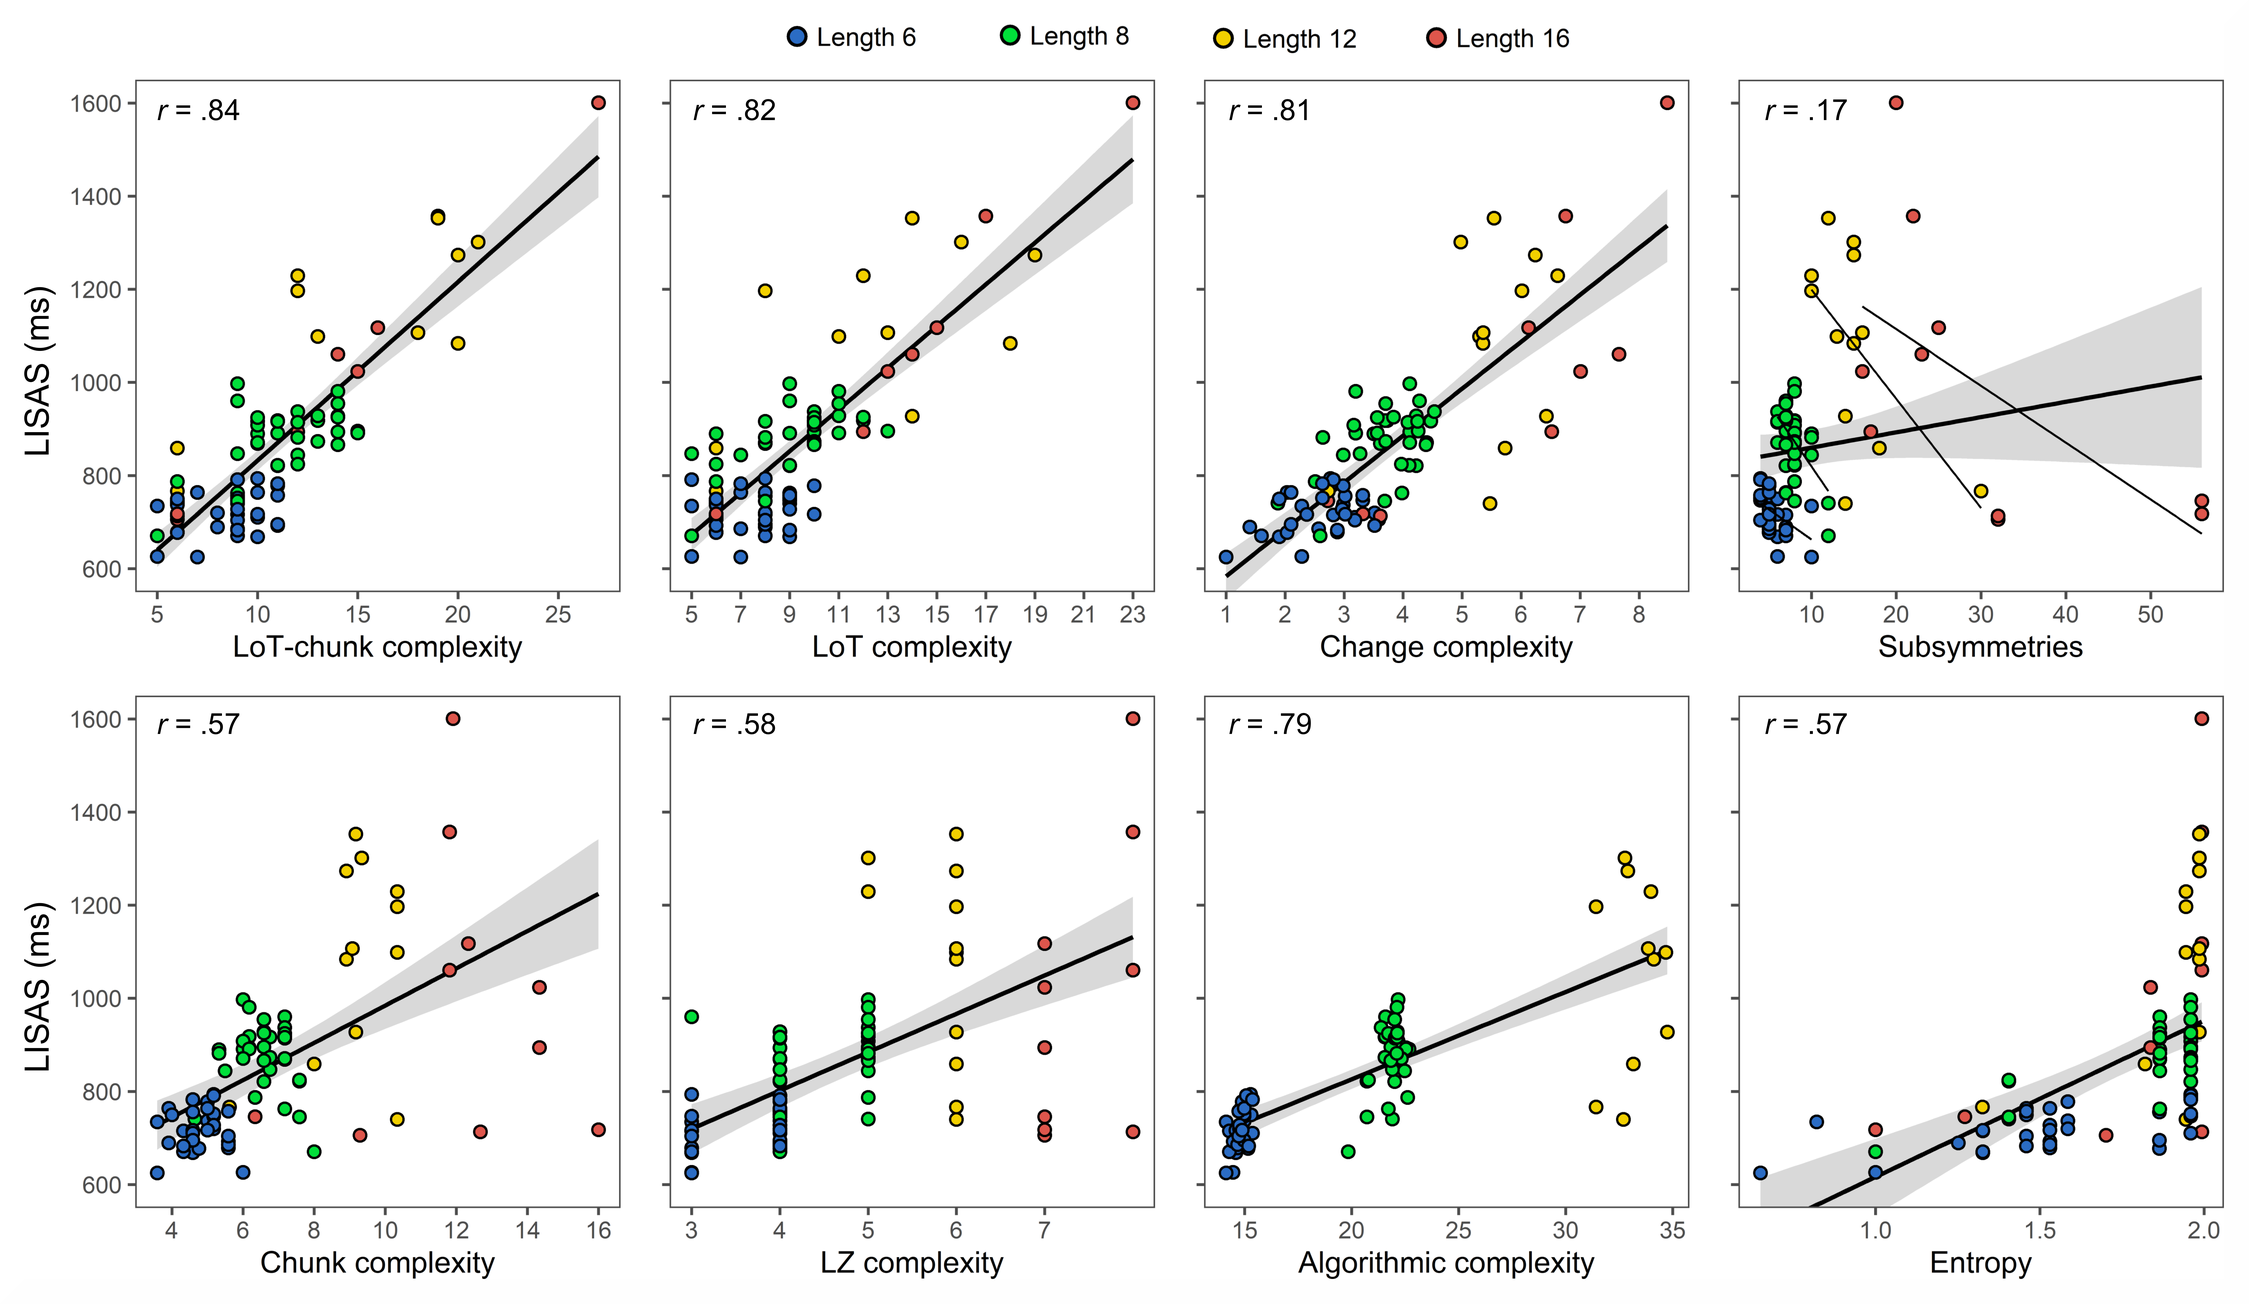
\includegraphics[scale=0.8]{figuras/plosbio/journal.pcbi.1008598.g009.PNG}
   
   \centering
   %%Figure 9: Linear regressions of average performance per sequence (LISAS, in ms) with eight different predictors of interest when combining data from experiments with auditory sequences of 4 different lengths. Each marker corresponds to one sequence. Sequences of different lengths are indicated by different markers only for illustration purposes (the length factor was not taken into account when computing the correlation coefficient, r). 16-items long sequences (as well as one 12-items sequence) could not be included in the regression with algorithmic complexity. Regressions lines for each sequence length were added in the subsymmetries plot, in order to illustrate the fact that negative correlations were observed when each length was considered separately. Note that the average performance data presented here does not take into account the effects of surprise, inter-subject, or inter-experiment variability.

   \caption{Regresiones lineas de rendimiento promedio por secuencia (LISAS, en ms.) con ocho predictores diferentes de interés al combinar datos de experimentos con secuencias auditivas de 4 longitudes diferentes. Cada marcador corresponde a una secuencia. Las secuencias de diferentes longitudes se indican con diferentes marcadores sólo a modo de ilustración (el factor de longitud no se tuvo en cuenta al calcular el coeficiente de correlación, r). Las secuencias de 16 elementos (así como una secuencia de 12 elementos) no se pudieron incluir en la regresión con complejidad algorítmica. Las líneas de regresión para cada longitud de secuencia se agregaron en el gráfico de subsimetrías con el fin de ilustrar que se observaron correlaciones negativas cuando se consideró cada longitud por separado. Notar que los datos de rendimiento promedio presentados aquí no tienen en cuenta los efectos de sorpresa o variabilidad entre sujetos o entre experimentos}
   \label{PlosBIO-F9}
\end{figure}
\sergio{la figura no está traducida}

\begin{figure}[t!]
   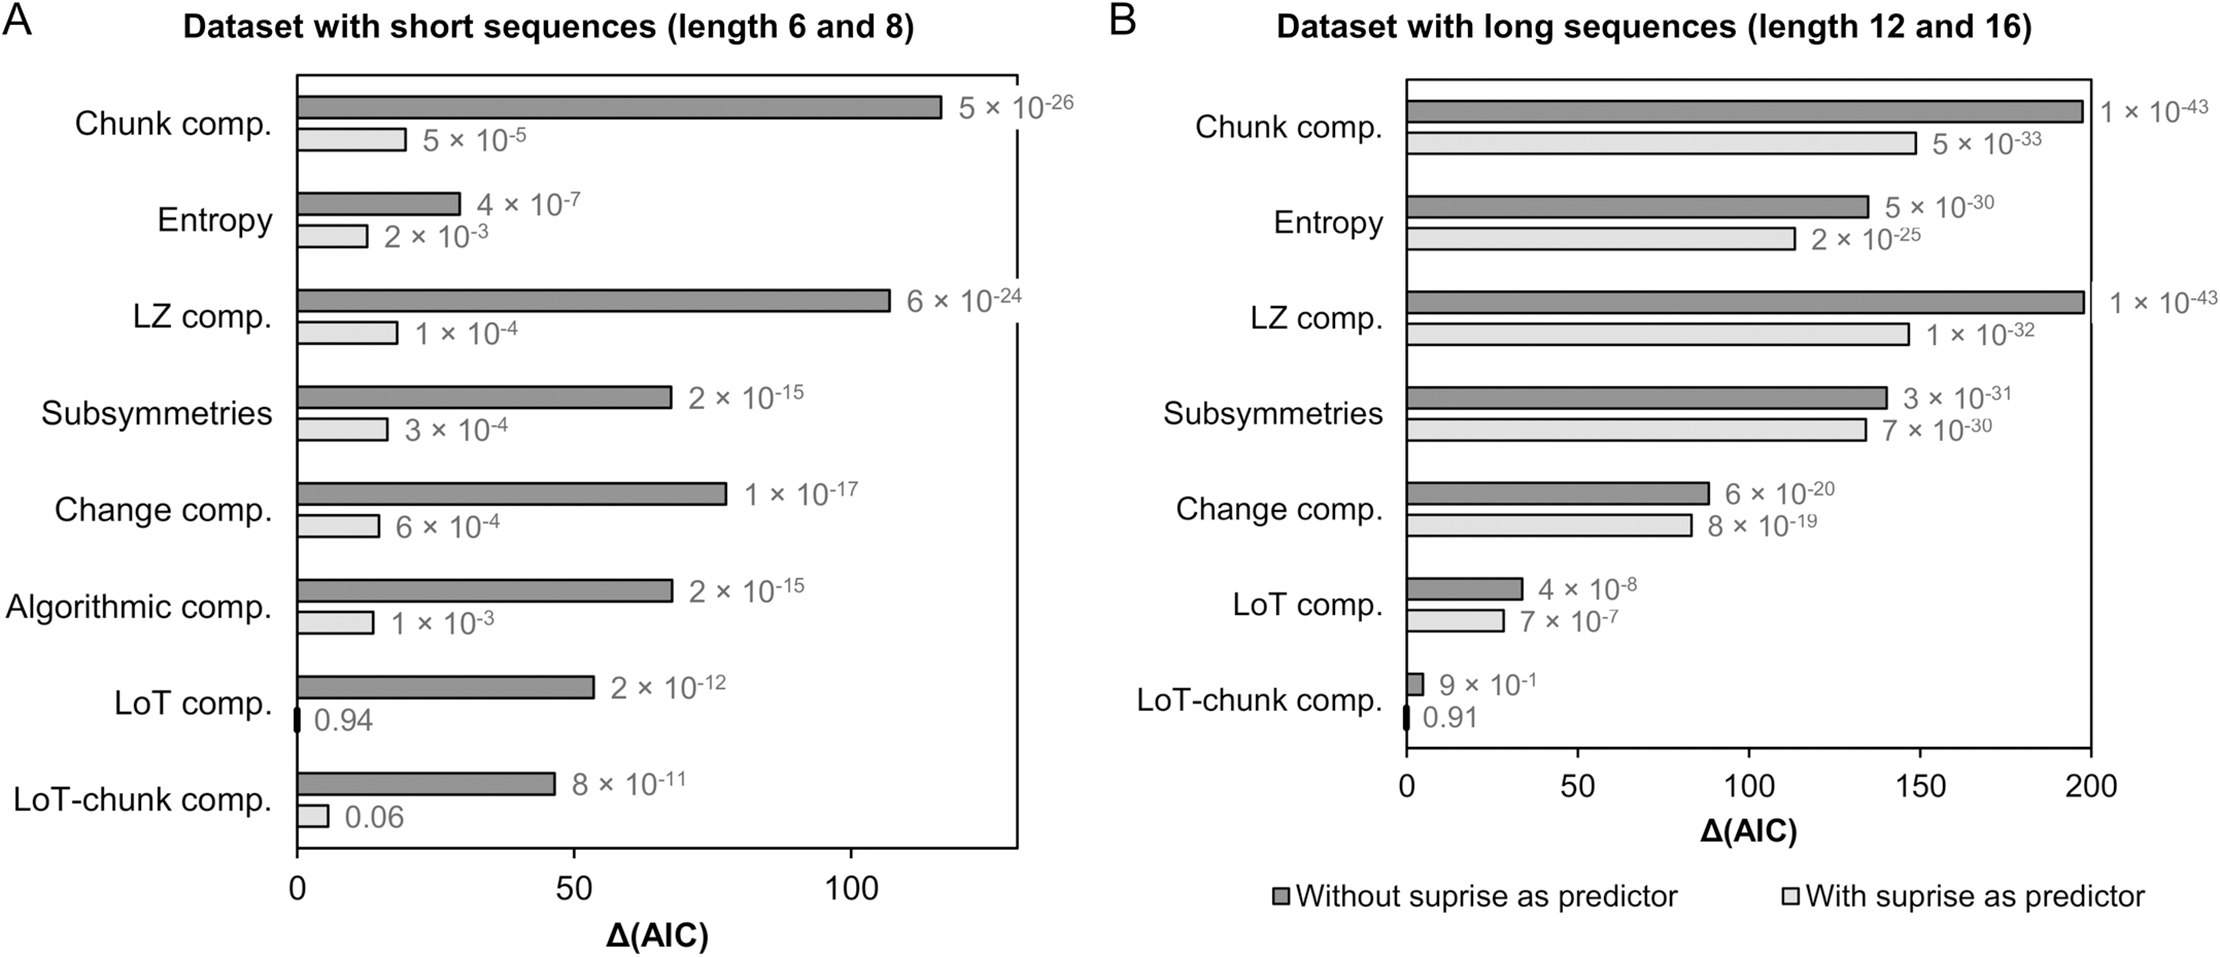
\includegraphics[scale=0.8]{figuras/plosbio/journal.pcbi.1008598.g010.PNG}
   
   \centering
   %%Figure 10: Complementary mixed model comparison with two pooled dataset. A) Δ(AIC) for the sixteen mixed models tested using a dataset including the task performance (LISAS) for sequences of length 6 and 8 (66 sequences) (A), and for the twelve different mixed models tested using the dataset with sequences of length 12 and 16 (22 sequences) (B). The fixed effect of interest is indicated along the vertical axis (all models included participants as a random effect and could include surprise as a covariate — light gray bars). Akaike weight for each model is also reported.
   
   \caption{Comparación de modelo mixto con dos conjuntos de datos. (A) $\Delta$ (AIC) para los dieciséis modelos mixtos probados usando un conjunto de datos que incluye el desempeño de la tarea (LISAS) para secuencias de longitud 6 y 8 (66 secuencias), y (B) para los doce modelos mixtos diferentes probados usando el conjunto de datos con secuencias de longitud 12 y 16 (22 secuencias). El efecto fijo de interés se indica a lo largo del eje vertical (todos los modelos incluyeron a los participantes como efecto aleatorio y podrían incluir la sorpresa como una covariable: barras de color gris claro). También se informa el peso de Akaike para cada modelo}
   \label{PlosBIO-F10}
\end{figure}
\sergio{la figura no está traducida}

\section{Discusión General}

%The main goal of this series of experiments was to evaluate the mental representation of binary sequences and to test the adequacy of a formal language of thought previously proposed to account for geometrical sequences (58). Similar models were proposed in the past (e.g. 32,36,45) but were not submitted to a full experimental validation, particularly in comparison to the most recent approaches of sequence complexity. Moreover, we sought to distinguish the effects related to statistical transition-probability learning, which are unavoidable when dealing with temporal sequences of stimuli, from the putative influence of rule-based encoding. Across five different experiments with sequences of different lengths, in the auditory but also in the visual modality, we found consistent evidence that, a significant part of the variations in sequence encoding performance (as indexed by the capacity to detect sequence violations) was explained by the length of the shortest possible description of the sequence in the proposed formal language (i.e. LoT complexity). This was however not the case for very short sequences (6 items). These results are consistent with the idea that upon hearing or seeing a binary sequence, when the number of items exceeds working memory capacity, subjects compress the sequence into an abstract, language-like mental representation. It is remarkable that a language merely composed of two simple instructions (“same” and “change”) and their recursive embeddings accounts for a large amount of the formation of such a representation. The complexity measure derived from this language was moreover better predictive of the degree of psychological complexity than other sophisticated approaches designed as alternatives to the non-computable Kolmogorov complexity (46,47). 

El objetivo principal de esta serie de experimentos fue evaluar la representación mental de secuencias binarias y probar la idoneidad de un lenguaje formal de pensamiento previamente propuesto para tener en cuenta las secuencias geométricas~\cite{amalric2017language}. Modelos similares fueron propuesto en el pasado (por ejemplo,~\cite{f32,f36,f45}), pero no fueron sometidos a una validación experimental completa, particularmente en comparación a los enfoques más recientes para la evaluación de la complejidad de las secuencias. Además, buscamos distinguir los efectos relacionados con el aprendizaje estadístico de las transiciones de probabilidad (que son inevitables cuando se trata de secuencias temporales de estímulos) de la supuesta influencia de la codificación basada en reglas. A través de cinco experimentos diferentes con secuencias de diferentes longitudes, en la modalidad auditiva pero también en la visual, encontramos evidencia consistente con que una parte significativa de las variaciones en el rendimiento de la codificación de secuencias (indexada según la capacidad para detectar violaciones de secuencias) se explicó por la longitud de la descripción más corta posible de la secuencia en el lenguaje formal propuesto (es decir, la complejidad LoT). Estos resultados son consistentes con la idea de que, al escuchar o ver una secuencia binaria, los sujetos forman una representación interna correspondiente a una forma abstracta y comprimida del contenido de la secuencia cuando el número de elementos excede la capacidad de la memoria de trabajo. Es notable que un lenguaje compuesto meramente por dos simples instrucciones (``mismo elemento'' y ``cambiar'') y sus anidamientos recursivos son suficientes para modelar la formación de tal representación. La medida de complejidad derivada de este lenguaje, de hecho, fue mejor predictor del grado de complejidad psicológica que otros enfoques sofisticados diseñados como alternativas a la complejidad no computable de Kolmogorov~\cite{f46,f47}.

%The assumption that the length of the shortest description in the formal language corresponds to perceived sequence complexity was further corroborated by subjective complexity rating (experiments 1 and 2). Moreover, we found that sequence structure was not the only information encoded by participants: surprise levels derived from the statistical estimation of transition probabilities also consistently explained part of the variance in violation detection performance. The effects of surprise and of complexity on responses to violations were found to vary differently depending on sequence length, thus providing new insights on how the human brain makes predictions in temporal sequences.

La suposición de que la longitud de la descripción más corta en el lenguaje formal corresponde a la complejidad percibida de la secuencia fue corroborada por la calificación de la complejidad subjetiva (experimentos 1 y 2). Además, encontramos que la estructura de la secuencia no era la única información codificada por los participantes, ya que el nivel de sorpresa derivado de la estimación estadística de las transiciones de probabilidad también ayudó consistentemente a explicar la variación en el rendimiento de detección de infracciones. Se encontró que los efectos de la sorpresa y la complejidad en las respuestas a las violaciones varían de manera diferente dependiendo de la longitud de la secuencia, lo que proporciona nueva información sobre cómo el cerebro humano hace predicciones en secuencias temporales

%The predictive power of the LoT was most notable for the longest sequences, in particular for 16 items long sequences (experiment 1; r = .98). Indeed, large differences in miss rates were observed between sequences predicted to be the least (AnBn patterns, with LoT complexity = 6) and the most complex (a set of 10 instructions, LoT complexity = 23), suggesting that subjects simply could not learn the latter efficiently (even after eight or more repetitions). An additional prediction of LoT was verified, namely the fact that the four sequences based on the AnBn pattern were associated with a similar performance level, regardless of n (= 1, 2, 4, or 8). In the language, this is because the complexity of a repetition is proportional to the log-number of repetitions (rounded up to the nearest integer). For a total number of 16 items, it therefore does not matter if the sequence is decomposed in 2 chunks of 8, 4 chunks of 4, 8 chunks of 2, or 16 chunks of 1: the sum of weights remains unchanged, leading to a LoT complexity of 6 bits in all cases — and indeed, the observed performance remained stable across such a broad variation ranging from huge chunks to pure alternation (see Figure 3). 

El poder predictivo del enfoque LoT fue más notable para las secuencias más largas, en particular para las secuencias de 16 elementos (experimento 1; $r = 98$). De hecho, se observaron diferencias altas en las tasas de fallos entre las secuencias que se predijeron como menos complejas (patrones $A^nB^n$, con complejidad LoT = 6) y las que se predijeron como más complejas (un conjunto de 10 instrucciones, con complejidad LoT = 23), lo que sugiere que los sujetos no pueden simplemente aprender estas últimas secuencias de manera eficiente, incluso después de ocho o más repeticiones. Una predicción adicional adicional sobre el LoT se verificó, el hecho de que las cuatro secuencias basadas en el patrón $A^nB^n$ se asociaron con un nivel de rendimiento similar, independientemente del n (= $1, 2, 4$ o $8$). En el lenguaje, esto se debe a que la complejidad de una repetición es proporcional al logaritmo del número de repeticiones, redondeado al número entero más próximo. Para un total de 16 elementos, por lo tanto, no importa cuándo si descompone la secuencia en 2 fragmentos de 8, 4 de 4, 8 de 2 o 16 de 1: la suma de los pesos permanece sin cambios, lo que lleva a una complejidad LoT de 6 bits en todos los casos, y de hecho, el desempeño observado se mantuvo estable a través de una variación tan amplia que va desde enormes fragmentos a puras alternancia (ver Figura~\ref{PlosBIO-F3}).

%The correlation of performance with LoT complexity decreased in subsequent experiments using increasingly shorter sequences, until it became almost absent for sequences comprising only six elements. Rather than an indication of an intrinsic limitation of the language for describing very short binary patterns, we believe that a significant part of this effect relates to differences in working memory demands. The number 6 indeed falls within the usual limits for the number of items that can be stored in working memory, which is around 7±2 items when there is no compression (16,29). Thus, subjects could have solved the violation detection task without compression, purely by storing each 6-items sequence “as is” in working memory. Similarly, 8-items sequences could have been stored as a mere flat series of “chunks”, which are thought to be the units of encoding in working memory (16,86,108,109), without any recursive embedding. All in all, an increasingly greater need to rely on compression would explain why the predictive power of LoT complexity increases with sequence length.

La correlación del rendimiento con la complejidad LoT disminuyó en experimentos posteriores al usar secuencias cada vez más cortas, hasta que se volvió casi ausente para las secuencias de sólo seis elementos. Más que una indicación de una limitación intrínseca del lenguaje para describir patrones binarios muy cortos, creemos que una parte significativa de este efecto se relaciona con las diferencias en las demandas de la memoria de trabajo. El número 6 de hecho cae dentro de los límites habituales para el número de elementos que se pueden almacenar en la memoria de trabajo, que es alrededor de $7 \pm 2$ elementos cuando no hay compresión~\cite{f16,f29}.Por lo tanto, los sujetos podrían haber resuelto la tarea de detección de violaciones sin compresión, puramente almacenando cada secuencia de 6 elementos en la memoria de trabajo. Del mismo modo, secuencias de 8 elementos podría haberse almacenado como una mera serie de ``fragmentos'', que se cree que son las unidades de la codificación en la memoria de trabajo~\cite{f16,f86,f108,f109}, sin anidamientos recursivos. A partir de esa longitud, una creciente necesidad de depender de la compresión explicaría por qué el poder predictivo de LoT aumenta con la longitud de la secuencia.

%Although the definition of working memory chunks as “a collection of elements having strong associations with one another” (25,110) is too vague to be rigorously tested using the present data, it is easy to imagine that both conceptions can lead to similar predictions (sequences composed of a small number of small chunks also have a short description in our language). Note however that, when considering all tested sequences, LoT complexity outperformed the “chunk complexity” predictor, for which chunks are defined using consecutive repetitions of the same item. In fact, a crucial feature of our theory lies in going beyond a simple concatenation of chunks and forming recursively embedded or nested representations, that is the ability to represent “chunks of chunks” or “repetitions of repetitions”. Indeed, the construction of recursively nested structured has been proposed as a core human ability, which sets us apart from other primates (4,6,7,111). Our results support the idea that the inclusion of such a feature is essential to explain human behavior when working memory capacity is exceeded and compression is most beneficial.

Aunque la definición de los fragmentos en la memoria de trabajo como ``una colección de elementos que tienen fuertes asociaciones entre sí''~\cite{f25,f110} es demasiado vaga para ser probada rigurosamente utilizando los datos presentes, es fácil imaginar que ambas concepciones pueden conducir a predicciones similares (secuencias compuestas por una pequeña cantidad de pequeños fragmentos también tienen una descripción breve en nuestro lenguaje). Sin embargo, se debe tener en cuente que, al considerar todas las secuencias probadas, la complejidad LoT superó al predictor de ``complejidad de fragmentos'', para el cual los fragmentos se definen mediante repeticiones consecutivas del mismo elemento. De hecho, una característica crucial de nuestra teoría radica en ir más allá de una simple concatenación de trazas y formar representaciones recursivamente incrustadas o anidadas, es decir, la capacidad de representar ``fragmentos de trazas'' o ``repeticiones de repeticiones''. De hecho, la construcción de estructuras recursivamente anidadas se ha propuesto como una habilidad humana central, que nos distingue de otros primates~\cite{f4,f6,f7,f111}. Nuestros resultados apoyan la idea de que la inclusión de dicha característica es esencial para explicar el comportamiento humano cuando se excede la capacidad de la memoria de trabajo y la compresión es más beneficiosa.

%The fact that we reached such a conclusion using the simplest type of temporal sequences (binary sequences) and a simple deviant detection task (rather than the more demanding recall, completion or production tasks using in the previous literature) is consistent with Fitch’s “dendrophilia hypothesis” (8) which states that “humans have a multi-domain capacity and proclivity to infer tree structures from strings” even in the simplest cases. The present work provides a foundation for future experiments in non-human primates, which would allow us to test the second aspect of this hypothesis, namely that this capacity for building recursive tree structures is only available to humans (4,6,8). In non-human primates, we postulate that a simpler language will suffice to account for sequence coding.

El hecho de que hayamos llegado a tal conclusión utilizando el tipo más simple de secuencias temporales (secuencias binarias) y con una simple tarea de detección de desviaciones (en lugar de las más exigentes tareas de recordar, completar o producir que se utilizan en otros trabajos de la literatura) es consistente con la \textit{hipótesis de la dendrofilia}~\cite{f8} que establece que los seres humanos tienen una propensión y una capacidad en múltiples dominios de inferir estructuras de árbol a partir de cadenas, incluso en los casos más simples. El presente trabajo proporciona una base para futuros experimentos en primates no humanos, lo que nos permitiría probar el segundo aspecto de esta hipótesis, a saber, que esta capacidad para construir estructuras de árboles recursivas solo está disponible para los humanos~\cite{f4,f6,f8}. En primates no humanos, postulamos que un lenguaje más simple será suficiente para explicar la codificación de secuencias.

%Numerous other frameworks for the estimation of pattern complexity have been proposed in the past, such as change complexity (47), algorithmic complexity (44–46), subsymmetries (94) or entropy (see also 34,96–98,111). These models are often based on quantitative aspects of information, such as the length, the number of transitions or runs, the probability of those transitions, the number of symmetries, or the number of changes. Although they all show some level of success in predicting behavior, they fail to capture recursive nesting, which as noted above seems to be an essential factor in human cognition (4,6). The same limitation applies to the Lempel-Ziv data compression algorithm, which compresses sequences by storing in memory a set of unique substrings that can occur at different locations in a sequence. Although it may seem psychologically relevant, this specific algorithm is unable to consider relationships between substrings mediated by an abstract, higher-level operation of repetition or change, as a LoT model does. In addition, this algorithm does not take advantage of contiguous repetitions. Conversely, the notion of repetition with variations is central to the success of our language. Others have also proposed that humans possess a “repetition detector”, as they are much better to learn repetition-based grammars than other forms of simple grammars (113). Such increased sensitivity for repetitions (compared to alternations) also follows from the simple assumption that humans track transition probabilities at a local scale (21). Repetition detection may already be present at birth, which suggests that it may be an innate neurocognitive function, perhaps essential for language acquisition (114). It may therefore not be surprising that nested repetitions with variations suffices to account for the human memory for sequences, and that models that do not incorporate this struggle to replicate human behavior.

Existen muchas propuestas para la estimación de la complejidad de patrones como la complejidad del cambio~\cite{f47}, la complejidad algorítmica D(5)~\cite{f44,f45,f46}, subsimetrías~\cite{f94} o la entropía~\cite{f34,f96,f97,f98,f111}. Estos modelos a menudo se basan en aspectos cuantitativos de la información, como la longitud, el número de transiciones o trazas, la probabilidad de esas transiciones, el número de simetrías o el número de cambios. Aunque todos muestran cierto nivel de éxito en la predicción del comportamiento, no logran capturar el anidamiento recursivo, que como señalamos arriba parecen ser un factor esencial en la cognición humana~\cite{f4,f6}. La misma limitación se aplica al algoritmo de compresión de datos Lempel-Zif, que comprime secuencias almacenando en la memoria un conjunto de subcadenas únicas que pueden ocurren en diferentes lugares en una secuencia. Aunque pueda parecer psicológicamente relevante, este algoritmo específico es incapaz de considerar las relaciones entre subcadenas mediadas mediante una operación abstracta de repetición o cambio de alto nivel, como lo hace un modelo de LoT. Además, este algoritmo no aprovecha las repeticiones contiguas. En cambio, la noción de repetición con variaciones es fundamental para el éxito de nuestro lenguaje. Otros trabajos han propuesto también que los humanos posean un \textit{detector de repetición}, ya que son mucho mejores para aprender gramáticas basadas en la repetición que otras formas de gramáticas simples~\cite{f113}. La detección de repetición puede estar ya presente al nacer, lo que sugiere que puede ser una función neurocognitiva innata, quizás esencial para la adquisición del lenguaje~\cite{f114}. Por lo tanto, puede que no sea sorprendente que la repetición anidada con variación basta para dar cuenta de la memoria humana para las secuencias, y que los modelos que no la incorporaran tengan dificultades para replicar el comportamiento humano.

%Following others in the domain of concept learning (e.g. 49,53), the approach adopted here assumes that binary sequences are encoded using a specific cognitive system that manipulates abstract, symbolic representations — a language of thought with recursive calls to a limited number of primitive operations. Thus, the present proposal does not merely provide a numerical value for complexity, but also parse trees and precise internal formats of representations, both of which could possibly be tested in future behavioral or brain-imaging experiments.

Siguiendo a otros en el dominio del aprendizaje de conceptos~\cite{piantadosi2012bootstrapping,piantadosi2016logical}, el enfoque adoptado aquí asume que las secuencias binarias se codifican utilizando un sistema cognitivo específico que manipula representaciones simbólicas abstractas, un lenguaje del pensamiento con llamadas recursivas a un número limitado de operaciones primitivas. Así, la presente propuesta no solo proporciona un valor numérico para la complejidad, sino también un árbol de derivación y un formato interno de representación preciso, los cuales posiblemente podrían ser probados en futuros experimentos conductuales o de imágenes cerebrales.

%Although the current study is based on the use of a “fixed” language, with predetermined rules and associated weights, some evidence suggests that a better description of human behavior can be achieved by incorporating a probabilistic component to the modeling attempt. This approach, advocated by Piantadosi & Jacobs (53) under the term probabilistic language of thought (pLOT), consists in using Bayesian probabilistic inference to estimate the likelihood of the existence of some set of rules (a proposed formal language), given the observed data. It has been shown to be especially efficient in modeling concept learning, for instance by replicating the patterns of errors throughout learning (50,52,56). This approach was also adopted to investigate how humans assess randomness in their environment. Human biases in subjective randomness judgments (e.g. 114,115) could be explained by assuming that the representation of randomness results from a statistical inference about the processes that generated the sequence (21), i.e. an estimation of the probability that a given regular process produced it (117). A good fit to human behavior was obtained without using the full power of Turing machines, but only finite-state automata with a stack, which are able to recognize repetitions, alternations or symmetries (18,117). Thus, despite fundamental differences (notably, deterministic versus probabilistic languages), the pLOT theory shares with our approach the need to consider similar types of primitive operations. Given the strong links between subjective randomness and complexity, we can reasonably expect that our formal language may also predict whether a pattern is perceived as random or not — a possibility which remains to be tested in future work.

\sergio{Tal vez este párrafo no tenga sentido en el contexto de esta tesis}
Aunque el estudio actual se basa en el uso de un lenguaje fijo, con reglas y pesos asociados, alguna evidencia sugiere que una mejor descripción del comportamiento se puede lograr incorporando un componente probabilístico al modelado. Este enfoque, defendido por~\cite{piantadosi2016four} bajo el término lenguaje de pensamiento probabilístico (pLoT), consiste en utilizar inferencia probabilística Bayesiana para estimar la probabilidad de la existencia de algún conjunto de reglas (un lenguaje formal propuesto), dada los datos observados. Se ha demostrado que es especialmente eficaz para modelar el aprendizaje de conceptos,por ejemplo, replicando los patrones de errores a lo largo del aprendizaje~\cite{goodman2008rational,piantadosi2012bootstrapping,piantadosi2016logical}. Este enfoque también se adoptó para investigar cómo los seres humanos evalúan la aleatoriedad en su entorno. Los sesgos humanos en los juicios subjetivos de aleatoriedad (\cite{f114,f115} podrían explicarse asumiendo que la representación de la aleatoriedad resulta de una inferencia estadística sobre los procesos que generaron la secuencia, es decir, una estimación de la probabilidad de que un proceso regular dado lo produjo~\cite{f21}. Un buen ajuste al comportamiento humano fue obtenido sin utilizar toda la potencia de las máquinas de Turing, sino simplemente autómatas de estado finito con una pila, que son capaces de reconocer la repetición, la alternancia o la simetría~\cite{f18,f117}. Por lo tanto, a pesar de las diferencias fundamentales (en particular, los lenguajes deterministas versus probabilísticos), la teoría pLOT comparte con nuestro enfoque la necesidad de considerar tipos similares de operaciones primitivas. Dados los fuertes vínculos entre aleatoriedad y complejidad subjetivas, podemos esperar razonablemente que nuestro lenguaje formal también puede predecir si un patrón se percibe como aleatorio o no; esta posibilidad permanece para ser probado en trabajos futuros.

%Beside the learning of conceptual knowledge and work on subjective randomness, a pLOT approach was also used to model the learning of spatial sequences: to study the crossmodal transfer of sequence knowledge (\cite{yildirim2015learning}), and to investigate the adequacy of the language of geometry (57). Indeed, by using the behavioral data from the octagon task of Amalric et al. (58), Romano et al. (57) showed that the primitives included in the language of geometry were all required in order to best account for human behavior. In spite of its successes, a number of questions and potential limitations of the LoT approach remain. First, the construction of our formal language implied methodological choices that could be considered as arbitrary or at least requiring more experimental validation. The primitive instructions included in our formal language were chosen for their alleged simplicity and because they suffice to represent any binary sequence. Other primitives could be tested (e.g. counting and a system of arithmetic; or temporal inversion or “mirroring”, see 10). Furthermore, modifications of the weights associated with each instruction or their number of repetitions may lead to different estimates of complexity. Finding the correct language for a given population is crucial, especially in the context of the debate on the uniqueness of human sequence processing skills, and specific statistical methodologies need to be developed for this purpose. As mentioned earlier, the pLOT approach which, using Bayesian inference, allows to find the most likely concepts and rules from a grammatically structured hypothesis space containing several candidates, appears to be a very promising approach for that purpose (50,53,57). Nevertheless, we also found that some of the minimal expressions produced by this language did not fit well with the way participants represent some sequences. The addition of the constraint that the minimal parse tree should respect the chunks or runs of consecutive repetitions, and never split any such chunk, was found to lead to a noticeable improvement in model fit. We speculate that this finding reflects the way participants build their internal representation of sequences: since the space of possible programs is immense, they would restrict the search to only those programs that, at the lowest level, generate the observed consecutive runs in the sequence. The perceptual dominance of the runs could act as a bottleneck, an initial grouping that would then restrict the sequence parsing process (as is sometimes assumed in some complexity estimation models; e.g. 98). A better characterization of this parsing process during sequence learning could help address the current limitations of our language.

\sergio{Acá también se explica el capítulo que viene. Ver de usarlo como continuidad}
Además del aprendizaje de conceptos y el trabajo sobre la aleatoriedad subjetiva, un enfoque pLoT también se utilizó para modelar el aprendizaje de secuencias espaciales: para estudiar la transferencia del conocimiento de secuencias entre ambientes~\cite{yildirim2015learning}, y para investigar la adecuación del lenguaje de la geometría~\cite{romano2018bayesian}. De hecho, al utilizar los datos de comportamiento de la tarea en el octágono de~\cite{amalric2017language}, Romano et al.~\cite{romano2018bayesian} mostraron que todas las primitivas incluidas en el lenguaje de la geometría eran necesarias para dar cuenta del comportamiento humano. A pesar de sus éxitos, una serie de preguntas y posibles limitaciones persisten en el enfoque LoT. Primero, la construcción de nuestro lenguaje formal implican elecciones metodológicas que podrían considerarse arbitrarias o al menos requerir mayores validaciones experimentales. Las instrucciones primitivas incluidas en nuestro lenguaje formal fueron elegidos por su supuesta simplicidad y porque son suficientes para representar cualquier secuencia binaria. Se podrían probar otras primitivas (por ejemplo, contar y un sistema de aritmético; o inversión temporal o espejo,~\cite{f10}). Además, las modificaciones de los pesos asociados con cada instrucción o su número de repeticiones puede llevar a diferentes estimaciones de complejidad. Encontrar el lenguaje correcto para una población determinada es crucial, especialmente en el contexto del debate sobre la singularidad de las habilidades humanas para el procesamiento de secuencias, y es necesario desarrollar metodologías estadísticas específicas para este fin. Como se mencionó anteriormente, el enfoque pLOT permite encontrar los conceptos y reglas más probables en un espacio de hipótesis estructurado gramaticalmente que contiene varios candidatos utilizando la inferencia Bayesiana, parece ser un enfoque muy prometedor para ese propósito~\cite{goodman2008rational,piantadosi2016four,romano2018bayesian}. Sin embargo, también encontramos que algunas de las expresiones mínimas producidas por este lenguaje no encajaban bien con la forma en que los participantes representan algunas secuencias. La adición de la restricción que el árbol de análisis mínimo debe respetar los fragmentos o las series de repeticiones consecutivas, y nunca dividir ninguno de esos fragmentos, se descubrió que conducía a una mejora notable en el ajusto del modelo. Especulamos que este hallazgo refleja la forma en que los participantes construyen su representación interna de las secuencias: dado que el espacio de posibles programas es inmenso, restringir la búsqueda a sólo aquellos programas que, en el nivel más bajo, generan las trazas consecutivas observadas en la secuencia. El peso de la percepción de las trazas podría actuar como un cuello de botella, una agrupación inicial que luego restringiría el proceso de análisis de la secuencia (como a veces se supone en algunos modelos de estimación de complejidad; véase, por ejemplo,~\cite{f98}). Una mejor caracterización de este proceso de análisis durante el aprendizaje de secuencias podría ayudar a abordar las limitaciones actuales de nuestro lenguaje.

%Another limitation is that, although we argued that the capacity to represent sequences using hierarchically embedded or nested descriptions is an essential feature of human behavior (4), about half of the minimal expressions for the sequences that we used included only two hierarchical levels (a single level of embedding; the average hierarchical depth was 2.5). Only a few sequences such as AABBABABAABBABA explicitly required repetitions of repetitions of repetitions. Although our model correctly predicted their subjective and objective complexity (see Figure 3), and although embedding is an effective compression process, more research is needed to probe whether human participants always consider such deep levels of embedding as beneficial in the processing of short sequences. Increasing the hierarchical depth may imply an additional processing cost, making it useful only in specific situations (e.g. for more demanding learning tasks or with long sequences).

Otra limitación es que, aunque argumentamos que la capacidad de representar secuencias utilizando descripciones con jerarquías o anidadas es una característica esencial del comportamiento humano~\cite{f4}, aproximadamente la mitad de las expresiones mínimas para las secuencias que usamos incluía solo dos niveles jerárquicos (el promedio de la profundidad jerárquica fue de 2.5). Solo unas pocas secuencias como AABBABABAABBABA requirieron explícitamente repeticiones de repeticiones de repeticiones. Aunque nuestro modelo correctamente predijo su complejidad subjetiva y objetiva (ver Figura~\ref{PlosBIO-F3}), y aunque el anidamiento es un proceso de compresión eficaz, se necesita más investigación para comprobar si los humanos siempre consideran beneficiosos niveles profundos de jerarquía para procesar secuencias auditivas cortas. Incrementar la profundidad jerárquica puede implicar un costo de procesamiento adicional, que sólo sea útil en situaciones específicas (por ejemplo, para tareas más exigentes de aprendizaje o con secuencias largas).

%Finally, our approach assumes that the mental compression of sequences does not necessarily occur at the level of the sensory items (i.e. grouping contiguous identical elements) but at the more abstract level of the relationships between items. Besides its success in predicting the psychological complexity of sequences of tones, one argument in favor of such an abstract symbolic representation is that it fitted equally well the complexity of visual sequences. However, it could be proposed that the mental encoding of temporal sequence does not involve any amodal, domain-general processing mechanisms, but rather two similarly organized modality-specific systems, or even a single modality-specific cognitive system dedicated to auditory processing; visual sequences would then be converted into an auditory representation prior to compression. Indeed, we observed a lower performance and slower responses in the visual compared to the auditory modality, a difference which has been postulated to reflect a dominance of the auditory system for the encoding of temporal information (91,118,119). One potential strategy for performing the task of experiment 5 with visual stimuli could have been a subvocal naming of the items, and a maintenance in working memory using the phonological loop (30,120). Further investigation is required to resolve these points, perhaps by relying on other sensory modalities, by testing transfer across modalities, or by using brain-imaging to determine the sensory versus higher-level nature of the brain mechanisms at play. We merely note here that activation of supra-modal prefrontal cortices has been reported during sequence processing (e.g. 19,60); that the existence of an automatic visual-to-auditory conversion in sequence processing has been challenged (121); and that the existence of an abstract representation of sequences as proposed here, allowing a transfer of knowledge across modalities, is already supported by some behavioral data (see 94).

Finalmente, nuestro enfoque asume que la compresión mental de secuencias no necesariamente ocurre en el nivel de los eventos sensoriales (es decir, agrupando elementos contiguos idénticos) pero en el nivel más abstracto de las relaciones entre eventos. Además de su éxito en predecir la complejidad psicológica de las secuencias de tonos, un argumento a favor de tal representación simbólica abstracta es que encaja igualmente bien con la complejidad de la secuencias binarias. Sin embargo, se podría proponer que la codificación mental de las secuencia no implica un mecanismo de procesamiento de dominio general, sino más bien dos sistemas específicos de modalidad organizados de manera similar, o incluso un único sistema cognitivo específica dedicado al procesamiento auditivo. Las secuencias visuales se convertirían entonces en una representación auditiva antes de la compresión. De hecho, observamos un desempeño más bajo y respuestas más lentas en la modalidad visual en comparación con la auditiva, una diferencia que ha sido postulado para reflejar un dominio del sistema auditivo para la codificación de información temporal~\cite{f91,f118,f119}. Se requiere otra investigación para resolver estos puntos, quizás apoyándose en otros modalidades, probando la transferencia a través de modalidades, o usando imágenes cerebrales para determinar la naturaleza sensorial en contraposición con el nivel superior de los mecanismos cerebrales en juego. Simplemente notamos aquí que la activación de cortezas prefrontales supramodales se ha informado durante la secuencia de procesamiento~\cite{f19,f60}; que la existencia de un conversión automática de lo visual a lo auditiva en el procesamiento de secuencias ha sido cuestionada~\cite{f121}; y que la existencia de una representación abstracta de secuencias como hemos planteado aquí, que permite una transferencia de conocimiento a través de modalidades, ya está respaldada por algunos datos de comportamiento~\cite{yildirim2015learning}.

%The violation detection task used in the present study implied the learning of a specific and deterministic sequence in each block, which was repeated multiple times with predictable timings. Our results, however, indicate that the statistical properties of the original sequence were also computed in parallel to the compression process and used for prediction, since, for a given sequence, performance varied according to the level of surprise, i.e. the negative log transition probability of the deviant sound in the context of the current sequence. For equal complexity, we observed a higher accuracy and faster response times for deviants that induced less frequent transitions. The observation that transition probability affects behavior even within a deterministic sequence (see also 80), as opposed to the stochastic sequences that were used in previous studies of statistical learning (e.g. 18–20,74,75,122), suggests that the learning of transition probabilities between items may occur automatically and in parallel to compression in working memory. This is compatible with the large amount of evidence showing that the brain encodes statistical regularities in sensory inputs in an implicit and unconscious manner (73,123–126). Since the effect of surprise occurred over and above any effect of sequence complexity, it also suggests that this statistical learning system is distinct from the more strategic system based on the learning of the deterministic sequence structure. Again, this is compatible with prior brain imaging results on the local-global paradigm, which indicate that the mismatch negativity (MMN), sensitive to local transition probability, can be dissociated from the P3b response associated with the acquisition of the global sequence (67,68,72).

La tarea de detección de violaciones utilizada en el presente estudio implicó el aprendizaje de una secuencia determinística específica en cada bloque, que se repitió varias veces con tiempos predecibles. Nuestros resultados, sin embargo, indican que las propiedades estadísticas de la serie original también se calcularon en paralelo al proceso de compresión y se utilizaron para la predicción, dado que para una secuencia dada, el rendimiento variaba de acuerdo con el nivel de sorpresa, es decir, el logaritmo negativo de las transiciones de probabilidad del sonido desviado en el contexto de la secuencia actual. Para igual complejidad, observamos una mayor precisión y tiempos de respuesta más rápidos para los desviados que inducían transiciones menos frecuentes. La observación de que la transición de probabilidad afecta el comportamiento incluso dentro de una secuencia determinística~\cite{f80}, en contraposición a las secuencias estocásticas que se utilizaron en estudios previos de aprendizaje estadístico~\cite{f18,f19,f20,f74,f75,f122}, sugiere que el aprendizaje de transiciones de probabilidad entre elementos puede ocurrir automáticamente y en paralelo a la compresión en la memoria de trabajo. Esto es compatible con la gran cantidad de evidencia que muestra que el cerebro codifica regularidades estadísticas en las entradas sensoriales de una manera implícita e inconsciente~\cite{f73,f123,f124,f125,f126}. Dado que el efecto de sorpresa se produjo por encima de cualquier efecto de complejidad de la secuencia, también sugiere que este sistema de aprendizaje estadístico es distinto del sistema más estratégico basado en el aprendizaje de la estructura secuencial determinista. Una vez más, esto es compatible con los resultados de imágenes cerebrales anteriores en el paradigma local-global, que indican que la negatividad de desajuste, sensible a los problemas locales de las probabilidades de transición, se puede disociar de la respuesta P3b asociada con la adquisición de la secuencia global~\cite{p67,p68,p72}.

%When pooling datasets from experiments with different sequence lengths, the linear mixed models with surprise and complexity as predictors fitted the data better than models including one predictor alone, indicating that those two predictors captured distinct aspects of the data. However, one may note that the size of the surprise effect varied across experiments. Surprise and complexity showed opposite patterns, with a stronger effect of complexity for longer sequences than shorter ones and, conversely, a strong effect of surprise only with the shortest sequences. Given the evidence that we just cited, showing that transition probabilities are constantly being computed unconsciously, the most likely interpretation is probably that task difficulty increased with sequence length and resulted in longer response times, thus masking the contribution of statistical learning. To test this idea, future work should use event-related potentials such as the MMN, which may provide a more sensitive measure of transition-probability learning. 

Al agrupar los conjuntos de datos de experimentos con diferentes longitudes de secuencia, la mezcla lineal de modelos con sorpresa y complejidad como predictores ajustaban los datos mejor que los modelos incluyendo un único predictor, lo que indica que esos dos predictores capturaron distintos aspectos de los datos. Sin embargo, se puede notar que el tamaño del efecto sorpresa varió entre los experimentos. La sorpresa y la complejidad mostraron patrones opuestos, con un efecto más fuerte de la complejidad para secuencias más largas que para las cortas y, a la inversa, un fuerte efecto de sorpresa solo con las secuencias más cortas. Dada la evidencia que acabamos de citar, que muestra esa las transiciones de probabilidad se calculan constantemente de forma inconsciente, la interpretación más probable es que la dificultad de la tarea aumentó con la longitud de la secuencia y resultó en mayores tiempos de respuesta, enmascarando así la contribución del aprendizaje estadístico y haciéndolo más difícil de detectar. 

%Finally, we found a complexity effect even when subjects responded to “súper-deviants” items, i.e. outlier sounds that could be detected without any knowledge of the sequence because their identity itself was novel. We suggest two putative interpretations of this unexpected effect. First, it could be due to the increased attentional load associated with more complex sequences. Essentially, participants would be placed in a dual-task situation of having to attend to two things are once: the complex sequence and the occasional deviants. In support of this idea, increased attentional load has indeed been found associated to sequence learning impairment in dual-task experiments (see 125). A second interpretation, within the predictive coding framework, is that deviance detection, even for extremely salient deviants, is easier for predictable than for unpredictable stimuli. Accordingly, Southwell and Chait (128) found larger brain responses evoked by deviant stimuli within a regular sequence than within a random sequence of tones. The authors propose that it could reflect a difference in the precision or predictability associated with the flow of sensory information. Indeed, in addition to the prediction regarding the content of incoming stimuli (manifested by prediction error signals), recent versions of predictive coding theories also formalize the concept of precision, which corresponds to the reliability of the prediction (80,129–132). Precision would manifest itself as a gain modulation of the relevant neural units (which is tightly related to attention), with increased precision leading to an increasing sensitivity to the predicted stimuli. This theory can explain the increased and sustained neuronal responses observed in a highly predictable context (126,128,129,133). The present complexity effect observed for súper-deviants may thus indicate that responses to completely unexpected events were modulated by the degree of predictability of the pattern, which itself depends upon the complexity of the pattern. A precision-weighting mechanism would thus explain why greater complexity leads to slower response times to any kind of violations in our violation detection task. Overall, the distinct contributions of surprise and complexity underline the joint contributions of statistical versus rule-based information in temporal sequence processing.

Finalmente, encontramos un efecto de complejidad incluso cuando los sujetos respondieron a las súper-desviaciones, es decir, a los sonidos atípicos que podrían detectarse sin ningún conocimiento de la secuencia porque su propia identidad era novedosa. Sugerimos dos interpretaciones de este efecto inesperado. Primero, podría deberse a la mayor carga de atención asociada con secuencias más complejas. Esencialmente, los participantes se colocarían en una situación de doble tarea, de tener que prestar atención a dos cosas en simultáneo: la secuencia compleja y las súper-desviaciones. En apoyo de esta idea, se ha encontrado una mayor carga de atención asociada al aprendizaje de secuencias en experimentos de doble tarea~\cite{f125}. Una segunda interpretación, dentro del marco de las teorías de codificación, es que la detección de desviaciones (incluso para desviaciones extremadamente importantes) es más fácil para estímulos predecibles que para estímulos impredecibles. De hecho, en~\cite{f128} encontraron una respuesta cerebral mayor a los estímulos de desviación dentro de una secuencia regular que dentro de una secuencia aleatoria de tonos. Los autores proponen que podría reflejar una diferencia en la precisión o previsibilidad asociada con el flujo de información sensorial. De hecho, además de la predicción sobre el contenido de estímulos entrantes (manifestados por señales de error de predicción), versiones recientes de las teorías de codificación, también formalizan el concepto de precisión, que corresponde a la confiabilidad de la predicción~\cite{f80,f129,f130,f131,f132}. La precisión se manifestaría como una ganancia en la modulación unidades neuronales relevantes (que está estrechamente relacionado con la atención), donde una mayor precisión conduciría a un aumento de la sensibilidad a los estímulos predichos. Esta teoría puede explicar el aumento sostenido de las respuestas neuronales observadas en un contexto altamente predecible~\cite{f126,f128,f129,f133}. El efecto de complejidad observado para las súper-desviaciones puede, por tanto, indicar que las respuestas a eventos completamente inesperados fueron modulados por el grado de predictibilidad del patrón, que a su vez depende de la complejidad del patrón. Un mecanismo de ponderación del peso de la precisión explicaría así por qué una mayor complejidad conduce a tiempos de respuesta más lentos para cualquier tipo de violación en nuestra tarea de detección de violaciones.

\subsection{Conclusión}

%Our study provides a first demonstration that, even after accounting for statistical transition probability learning, responses to sequence violations can be used to uncover the properties of the abstract mental language used by individuals to encode sequential patterns. The present proposal, which takes the form of a psychologically plausible formal language composed of a restricted set of simple rules (conforming to a simplicity principle and especially relying on the human ability to detect repetitions), proved to be more effective than alternative approaches in modeling the human memory for simple sequences. The observed relationship between sequence complexity and performance in the detection of violations is consistent with the idea that the brain acts as a compressor of incoming information that captures regularities and uses them to predict the remainder of the sequence. The present non-verbal passive paradigm paves the way to future neurophysiological recording studies that would probe the similarities and differences between humans and other species (13) or test the abilities of preverbal infants (70). A fundamental question for future research is whether the same formal language can explain sequence processing in other primate species, or if such a language is unique to humans (6).

Nuestro estudio proporciona una primera demostración de que, incluso después de tener en cuenta las probabilidades de transición, las respuestas a las violaciones de secuencia se pueden utilizar para descubrir las propiedades del lenguaje abstracto del pensamiento utilizado por los individuos para codificar patrones secuenciales. La presente propuesta, que toma la forma de un lenguaje formal psicológicamente plausible compuesto por un conjunto restringido de reglas simples, demostró ser más eficaz que los enfoques alternativos en el modelado de la memoria humana para secuencias simples. La relación observada entre la complejidad de la secuencia y el desempeño en la detección de violaciones es coherente con la idea de que el cerebro actúa como un compresor de información entrante que captura regularidades y las usa para predecir el resto de la secuencia. El presente paradigma pasivo y no verbal allana el camino para futuros estudios de registros neurofisiológicos que podrían probar las similitudes y diferencias entre los humanos y otras especies~\cite{f13} o probar las habilidades de los bebés preverbales~\cite{f70}. Una pregunta fundamental para las investigaciones futuras es si el mismo lenguaje formal puede explicar el procesamiento de secuencias en otras especies de primates, o si tal lenguaje es exclusivo de los humanos~\cite{f6}.

    %!TEX root = ../main.tex

%\section*{Abstract}
%Probabilistic proposals of Language of Thoughts (LoTs) can explain learning across different domains as statistical inference over a compositionally structured hypothesis space. While frameworks may differ on how a LoT may be implemented computationally, they all share the property that they are built from a set of atomic symbols and rules by which these symbols can be combined.
%In this work we propose an extra validation step for the set of atomic productions defined by the experimenter. It starts by expanding the defined LoT grammar for the cognitive domain with a broader set of arbitrary productions and then uses Bayesian inference to prune the productions from the experimental data. The result allows the researcher to validate that the resulting grammar still matches the intuitive grammar chosen for the domain. We then test this method in the \textit{language of geometry}, a specific LoT model for geometrical sequence learning. Finally, despite the fact of the geometrical LoT not being a universal (i.e. Turing-complete) language, we show an empirical relation between a sequence's {\em probability} and its {\em complexity} consistent with the theoretical relationship for universal languages described by Levin's Coding Theorem.

\chapter{Validación bayesiana de producciones gramaticales para el lenguaje del pensamiento}\label{chapter:PO}
\chaptermark{Validación bayesiana de gramáticas}


%Most studies of LoTs have focused on the compositional aspect of the language, which has either been modeled within a Bayesian~\cite{tenenbaum2011grow} or a Minimum Description Length (MDL) framework~\cite{amalric2017language,goldsmith2002probabilistic,romano2013language,goldsmith2001unsupervised}.

La mayoría de los estudios de \lot se han centrado en el aspecto compositivo del lenguaje, modelando la composición a través de técnicas de inferencia bayesiana~\cite{tenenbaum2011grow} o de longitud mínima de descripción (MDL, por sus siglas en inglés)~\cite{amalric2017language,goldsmith2002probabilistic,romano2013language,goldsmith2001unsupervised}.

%The common method is to define a grammar with a set of productions based on operations that are intuitive to researchers and then study how different inference processes match regular patterns in human learning. A recent study~\cite{piantadosi2016logical} puts the focus on the process of how to empirically choose the set of productions and how different LoT definitions can create different patterns of learning. Here, we move along that direction but use Bayesian inference to individuate the LoT instead of comparing several of them by hand.

El método más común es definir una gramática con un conjunto de producciones basadas en operaciones que son intuitivas para los investigadores y luego estudiar cómo diferentes procesos de inferencia coinciden con los patrones del aprendizaje humano. Un estudio reciente~\cite{piantadosi2016logical} pone el foco en el proceso de cómo elegir empíricamente el conjunto de producciones y cómo diferentes definiciones del \lot pueden crear diferentes patrones de aprendizaje. En este trabajo, encaramos esa dirección pero utilizando la inferencia bayesiana para seleccionar el \lot en lugar de seleccionarlo a partir de la comparación empírica de las distintas versiones con los patrones a replicar.


%Broadly, our aim is to propose a method to select the set of atomic symbols in an inferential process by pruning and trimming from a broad repertoire. More precisely, we test whether Bayesian inference can be used to decide the proper set of productions in a LoT defined by a context free grammar. These productions are derived from the subjects' experimental data. In order to do this, a researcher builds a broader language with two sets of productions: 1) those for which she has a strong prior conviction that they should be used in the cognitive task, and 2) other productions that could be used to structure the data and extract regularities even if she believes are not part of the human reasoning repertoire for the task. With the new broader language, she should then turn the context free grammar that defines it into a probabilistic context free grammar (PCFG) and use Bayesian analysis to infer the probability of each production in order to choose the set that best explains the data.

En términos generales, nuestro objetivo es proponer un método para seleccionar el conjunto de símbolos atómicos en un proceso de inferencia, seleccionándolos y recortándolos de un repertorio más amplio. Más precisamente, nos interesa probar si la inferencia bayesiana puede utilizarse para decidir el conjunto adecuado de producciones en un \lot definido por una gramática libre de contexto, derivando las producciones a elegir de los datos experimentales de los sujetos del experimento. Para hacer esto, un investigador debería construir un lenguaje suficientemente amplio con dos conjuntos de producciones: 1) aquellas para las que tiene una fuerte convicción previa de que podrían ser utilizadas en la tarea cognitiva a estudiar, y 2) otras producciones que podrían utilizarse para estructurar los datos y extraer regularidades incluso si cree que no son parte del repertorio de razonamiento humano para la tarea. Con el nuevo lenguaje más amplio, debería convertir la gramática libre de contexto que lo define en una gramática probabilística libre de contexto (PCFG, por sus siglas en inglés) y utilizar el análisis bayesiano para inferir la probabilidad de cada producción y, así, el conjunto que mejor explique los datos.

%In the next section we formalize this procedure and then apply it on the \textit{language of geometry} presented by Amalric et al. in a recent study about geometrical sequence learning~\cite{amalric2017language}. This LoT defines a language with some basic geometric instructions as the grammar productions and then models their composition within the MDL framework. Our method, however, can be applied to any LoT model that defines a grammar, independently of whether its compositional aspect is modeled using a Bayesian framework or a MDL approach.

En la siguiente sección, formalizaremos este procedimiento, que luego lo aplicaremos en \gramgeo. Nuestro método, sin embargo, se puede aplicar a cualquier modelo de \lot que defina una gramática, independientemente de si su aspecto compositivo se modela utilizando un enfoque de probabilidad bayesiana o de MDL.

%Finally, even with the recent surge of popularity of Bayesian inference and MDL in cognitive science, there are --to the best of our knowledge-- no practical attempts to close the gap between probabilistic and complexity approaches to LoT models.

Finalmente, incluso con el reciente aumento de popularidad de la inferencia bayesiana y el MDL en la ciencia cognitiva, no hay --hasta donde sabemos-- intentos prácticos de cerrar la brecha entre ambos enfoques.

%The theory of computation, through Levin's Coding Theorem~\cite{levin1974laws}, exposes a remarkable relationship between the {\em Kolmogorov complexity} of a sequence and its {\em universal probability}, largely used in algorithmic information theory. Although both metrics are actually non-computable and defined over a universal prefix Turing Machine, we can apply both ideas to other non-universal Turing Machines in the same way that the concept of complexity used in MDL can be computed for specific, non-universal languages.

La teoría de la computabilidad, a través del Teorema de Codificación de Levin~\cite{levin1974laws}, expone una notable relación entre la {\em complejidad de Kolmogorov} de una secuencia (que es la base del cálculo del MDL) y su {\em probabilidad universal}, la cual es ampliamente utilizada en la teoría algorítmica de la información. Aunque ambas métricas resultan no computables y se encuentran definidas sobre una Máquina Universal de Turing libre de prefijos, podemos aplicar estas ideas a otras Máquinas de Turing no universales de la misma manera que el concepto de complejidad es utilizado para el cálculo de MDL en lenguajes específicos no universales. \santi{referenciar capítulo correspondiente de intro}

%In this work, we examine the extent to which this theoretical prediction for infinite sequences holds empirically for a specific LoT, the \textit{language of geometry}. Although the inverse logarithmic relationship between both metrics is proved for universal languages in the Coding Theorem, testing this same property for a particular non-universal language shows that the language shares some interesting properties of general languages. This constitutes a first step towards a formal link between probability and complexity modeling frameworks for LoTs.

En este trabajo también examinamos hasta qué punto esta predicción teórica para secuencias infinitas se preserva empíricamente para un \lot específico, \gramgeo. Aunque la relación logarítmica inversa entre ambas métricas está probada para lenguajes universales en el Teorema de Codificación, probar esta misma propiedad para un lenguaje no universal particular muestra que el lenguaje comparte algunas propiedades interesantes con los lenguajes generales. Esto constituye un primer paso hacia un vínculo formal entre el modelado de probabilidad y el de complejidad para el \lot.

%\section{Bayesian inference for LoT's productions}
\section{Inferencia bayesiana para las producciones del \lot}

%The project of Bayesian analysis of the LoT models concept learning using Bayesian inference in a grammatically structured hypothesis space~\cite{goodman2008rational}. Each LoT proposal is usually formalized by a context free grammar $\gram$ that defines the valid functions or programs that can be generated, like in any other programming language. A program is a derivation tree of $\gram$ that needs to be interpreted or executed according to a given semantics in order to get an actual description of the concept in the cognitive task at hand. Therefore, each concept is then represented by any of the programs that describe it and a Bayesian inference process is defined in order to infer from the observed data the distribution of valid programs in $\gram$ that describes the concepts.

El proyecto de análisis bayesiano del \lot modela el aprendizaje de conceptos utilizando la inferencia bayesiana en un espacio de hipótesis estructurado a partir de una gramática~\cite{goodman2008rational}. Cada propuesta de \lot suele formalizarse mediante una gramática libre de contexto $\gram$ que define las funciones o programas válidos que se pueden generar, como en cualquier otro lenguaje de programación. Aquí, un programa es un árbol de derivación de $\gram$ que necesita ser interpretado o ejecutado de acuerdo a una semántica dada para obtener una descripción real del concepto en la tarea cognitiva en cuestión. Por lo tanto, cada concepto puede ser representado por cualquiera de los programas que lo describen al ejecutarse, y un proceso de inferencia bayesiano es definido para calcular la distribución de los programas válidos de $\gram$ que describen los conceptos a explicar.

%As explained above, our aim is to derive the productions of $\gram$ from the data, instead of just conjecturing them using a priori knowledge about the task. Prior work on LoTs has fit probabilities of productions in a context free grammar using Bayesian inference, however, the focus has been put in integrating out the production probabilities to better predict the data without changing the grammar definition~\cite{piantadosi2016logical}. Here, we want to study if the inference process could let us decide which productions can be safely pruned from the grammar. We introduce a generic method that can be used on any grammar to select and test the proper set of productions. Instead of using a fixed grammar and adjusting the probabilities of the productions to predict the data, we use Bayesian inference to rule out productions with probability lower than a certain threshold. This allows the researcher to validate the adequacy of the productions she has chosen for the grammar or even define one that is broad enough to express different regularities and let the method select the best set for the observed data.

Como se explicó anteriormente, nuestro objetivo es derivar las producciones de $\gram$ a partir de los datos, en lugar de sólo conjeturarlas utilizando un conocimiento a priori sobre la tarea. Otros trabajos previos en \lot ajustaron las probabilidades de las producciones de las gramáticas libres de contexto utilizando inferencia bayesiana~\cite{piantadosi2016logical}, sin embargo, han puesto el foco en la integración de las probabilidades de producción para predecir mejor los datos y no en cambiar la definición de las gramáticas. Aquí queremos estudiar si el proceso de inferencia podría permitirnos decidir qué producciones de la gramática pueden podarse con seguridad. Para esto, introducimos un método genérico que puede utilizarse en cualquier gramática para seleccionar y probar el conjunto adecuado de producciones. En lugar de usar una gramática fija y ajustar las probabilidades de las producciones para predecir los datos, utilizamos la inferencia bayesiana para remover las producciones con una probabilidad inferior a cierto umbral. Esto permite al investigador validar la adecuación de las producciones que ha elegido para la gramática o incluso definir una que sea lo suficientemente amplia como para expresar diferentes regularidades y dejar que el método seleccione el mejor conjunto a partir de los datos observados.   


%To infer the probability for each production based on the observed data, we need to add a vector of probabilities $\theta$ associated with each production in order to convert the context free grammar $\gram$ into a probabilistic context free grammar (PCFG)~\cite{manning1999foundations}.

Para inferir la probabilidad de cada producción a partir de los datos observados, necesitamos agregar un vector de probabilidades $\theta$ asociado con cada producción para convertir a la gramática libre de contexto $\gram$ en una gramática probabilística libre de contexto (PCFG)~\cite{manning1999foundations}.

%Let $D = (d_1, d_2, \dots, d_n)$ denote the list of concepts produced by the subjects in an experiment. This means that each $d_i$ is a concept produced by a subject in each trial. Then, $P(\theta \mid D)$, the posterior probability of the weights of each production after the observed data, can be calculated by marginalizing over the possible programs that compute $D$:

Sea $D = (d_1, d_2, \dots, d_n)$ la lista de conceptos obtenida de los sujetos en un experimento. Esto significa que cada $d_i$ es un concepto generado por un sujeto en cada ensayo. Luego, $P(\theta \mid D)$, la probabilidad a posteriori de los pesos de cada producción después de observar los datos, se puede calcular marginalizando sobre los posibles programas que computan $D$:
%
\begin{equation*}
\label{eqA}
P(\theta \mid D) = \sum_{\Prog } P(\Prog,\theta \mid D),
\end{equation*} donde cada $\Prog  = (p_1, p_2, \cdots, p_n)$ es un posible conjunto de programas tales que cada $p_i \in \gram$ computa el correspondiente concepto $d_i$ a partir de la semántica definida para la gramática, $\sem{p_i} = d_i$
%where each $\Prog  = (p_1, p_2, \cdots, p_n)$ is a possible set of programs such that each $p_i$ computes the corresponding concept $d_i$.

%We can use Bayesian inference to learn the corresponding programs $\Prog$ and the vector $\theta$ for each production in the grammar, applying Bayes rule in the following way:
Podemos usar la inferencia bayesiana para aprender los programas correspondientes $\Prog$ y el vector $\theta$ para cada producción de la gramática, aplicando la regla de Bayes de la siguiente manera:
%
\begin{equation}
\label{eq:mainB}
P(\Prog,\theta \mid D) \propto P(D \mid \Prog)\ P(\Prog \mid \theta)\ P(\theta),
\end{equation}
%

%Sampling the set of programs from $P(\Prog \mid \theta)$ forces an inductive bias which is needed to handle uncertainty under sparse data. Here we use a standard prior for programs that is common in the LoT literature to introduce a syntactic complexity bias that favors shorter programs~\cite{goodman2008rational,overlan2017learning}. Intuitively, the probability of sampling a certain program is proportional to the product of the production rules that were used to generate such program, and therefore inversely proportional to the size of the derivation tree. Formally, it is defined as:

Hacer un muestreo del conjunto de programas de $P(\Prog \mid \theta)$ fuerza un sesgo inductivo que es necesario para manejar la incertidumbre frente a datos escasos. Aquí usamos como probabilidad a priori para los programas un estándar que es común en la literatura de \lot para introducir un sesgo de complejidad sintáctica que favorece programas más cortos~\cite{goodman2008rational,overlan2017learning}. Intuitivamente, la probabilidad de muestreo de un determinado programa es proporcional al producto de las reglas de producción que se utilizaron para generar dicho programa y, por lo tanto, inversamente proporcional al tamaño del árbol de derivación. Formalmente, se define como:
%
\begin{equation*}
\label{eqC}
P(\Prog \mid \theta)\ = \prod\limits_{i = 1}^n P(p_i \mid \theta),
\end{equation*}
%
donde $P(p_i \mid \theta) = \prod\limits_{r \in \gram} \theta^{f_r(p_i)}_{r}$ es la probabilidad del programa $p_i$ en la gramática, y $f_r(p_i)$ es el número de ocurrencias de la producción $r$ en el programa $p_i$.
%where $P(p_i \mid \theta) = \prod\limits_{r \in G} \theta^{f_r(p_i)}_{r}$ is the probability of the program $p_i$ in the grammar, and $f_r(p_i)$ is the number of occurrences of the production $r$ in program $p_i$.

%In \eqref{eq:mainB}, $P(\theta)$ is a Dirichlet prior over the productions of the grammar. By using the term $P(\theta)$ we are abusing notation for simplicity. The proper term would be $P(\theta \mid \alpha)$ to express a Dirichlet prior with $\alpha \in \mathbb{R}^\ell$ its associated concentration vector hyper-parameter where $\ell$ is the number of productions in the grammar. This hierarchical Dirichlet prior has sometimes been replaced with a uniform prior on productions as it shows no significant differences in prediction results~\cite{piantadosi2012bootstrapping,yildirim2015learning}. However, here we will use the Dirichlet prior to be able to infer the production probabilities from this more flexible model.

En la ecuación \eqref{eq:mainB}, $P(\theta)$ es una Dirichlet que se utiliza como distribución a priori sobre las producciones de la gramática. Al utilizar el término $P(\theta)$ estamos abusando de la notación por simplicidad. El término adecuado sería $P(\theta \mid \alpha)$ para expresar la distribución a priori con $\alpha \in \mathbb{R}^\ell$ su hiperparámetro que actúa como vector de concentración asociado, donde $\ell$ es el número de producciones de la gramática. Esta distribución a proiri ha sido también reemplazada por una distribución uniforme, ya que no muestra diferencias significativas en resultados de predicción~\cite{piantadosi2012bootstrapping,yildirim2015learning}. Sin embargo, aquí utilizaremos la distribución Dirichlet para poder inferir las probabilidades de producción a partir de este modelo más flexible.

%The likelihood function is straightforward. It does not use any free parameter to account for perception errors in the observation. This forces that only programs that compute the exact concept are taken into account, and it can be easily calculated as follows:

La función de verosimilitud es sencilla. No utiliza ningún parámetro libre para contabilizar errores de percepción en la observación. Esto obliga a que sólo los programas que computan el concepto exacto se tengan en cuenta, y puede ser fácilmente calculada de la siguiente manera:
%
\begin{equation*}
\label{eqD}
P(D \mid \Prog)\ = \prod\limits_{i = 1}^n P(d_i \mid p_i),
\end{equation*}
%
%where $P(d_i \mid p_i) = 1 $ if the program $p_i$ computes $d_i$, and 0 otherwise.
donde $P(d_i \mid p_i) = 1 $ si $\sem{p_i} = d_i$ (el programa $p_i$ computa $d_i$), y 0 en caso contrario. 
%Calculating $P(\theta \mid D)$ directly is, however, not tractable since it requires to sum over all possible combinations of programs $\Prog$ for each of the possible values of $\theta$. To this aim, then, we used a Gibbs Sampling~\cite{geman1984stochastic} algorithm for PCFGs via Markov Chain Monte Carlo (MCMC) similar to the one proposed at~\cite{johnson2007bayesian}, which alternates in each step of the chain between the two conditional distributions:

Sin embargo, calcular $P(\theta \mid D)$ de manera directa no es computacionalmente tratable ya que requiere sumar todas las posibles combinaciones de programas $\Prog$ para cada uno de los posibles valores de $\theta$. Para este objetivo, utilizamos entonces el algoritmo de muestreo de Gibbs~\cite{geman1984stochastic} para PCFGs a través del Método de Monte Carlo basado en cadenas de Markov (MCMC, por sus siglas en inglés) similar al propuesto en~\cite{johnson2007bayesian}, el cual alterna en cada paso de la cadena entre las dos distribuciones condicionales:\santi{no sé si se entiende 'el cual alterna en cada paso de la cadena entre las dos distribuciones condicionales'} \sergio{Te parece que cuente en la intro cómo funciona el MCMC? O hago una pequeña aclaración de que se va sampleando de manera alternada de cada distribución hasta que converjan?}
%
\begin{eqnarray*}
\label{eqE}
P(\Prog \mid \theta, D) &=& \prod\limits_{i=1}^n P(p_i \mid d_i, \theta).\\
P(\theta \mid \Prog, D) &=& P_D(\theta \mid f(\Prog) + \alpha).
\end{eqnarray*}
%Here, $P_D$ is the Dirichlet distribution where the positions of the vector $\alpha$ were updated by counting the occurrences of the corresponding productions for all programs $p_i \in \Prog$.
Aquí, $P_D$ es la distribución Dirichlet donde las posiciones del vector $\alpha$ fueron actualizadas contando las ocurrencias de las producciones correspondientes para todos los programas $p_i \in \Prog$.

%In the next section, we apply this method to a specific LoT. We add a new set of ad-hoc productions to the grammar that can explain regularities but are not related to the cognitive task. Intuitively, these ad-hoc productions should not be part of the human LoT repertory, still all of them can be used in many possible programs to express each concept.

En la siguiente sección, aplicamos este método a \gramgeo. Agregamos un nuevo conjunto ad-hoc de producciones a la gramática original que pueden explicar regularidades pero que no están relacionadas con la tarea cognitiva del problema original. Intuitivamente, estas producciones ad-hoc no deberían formar parte del repertorio de \gramgeo, aún así, todas ellas pueden usarse en muchos programas posibles para expresar cada uno de los conceptos.

%So far, Probabilistic LoT approaches have been successful to model concept learning from few examples~\cite{tenenbaum2011grow,piantadosi2016four}. However, this does not mean that Bayesian models would be able to infer the syntax of the model's grammar from sparse data. Here we test such hypothesis. If the method is effective, it should assign a low probability to the ad-hoc productions and instead favor the original set of productions selected by the researchers for the cognitive task. This would not only provide additional empirical evidence about the adequacy of the choice of the original productions for the selected LoT but, more importantly, about the usefulness of Bayesian inference for validating the set of productions involved in different LoTs.

Hasta ahora, los enfoques probabilísticos del \lot han tenido éxito para modelar el aprendizaje de conceptos a partir de pocos ejemplos~\cite{tenenbaum2011grow,piantadosi2016four}. Sin embargo, esto no significa que los modelos bayesianos puedan inferir la sintaxis de la gramática a partir de datos escasos. Aquí probamos esta hipótesis. Si el método es eficaz, debería asignar una probabilidad baja las producciones ad-hoc y en su lugar favorecer el conjunto original de producciones seleccionadas por los investigadores para la tarea cognitiva. Esto no sólo proporcionaría evidencia empírica adicional sobre la idoneidad de la elección original de producciones para el \lot, sino que --más importante-- brindaría evidencia sobre la utilidad de la inferencia bayesiana para validar el conjunto de producciones involucradas en diferentes LoTs. 

%\section{The Language of Geometry: $\gramgeo$}
\section{El lenguaje de geometría: $\gramgeo$}

%The \textit{language of geometry}, $\gramgeo$~\cite{amalric2017language}, is a probabilistic generator of sequences of movements on a regular octagon like the one in Figura~\ref{fig:circle}. It has been used to model human sequence predictions in adults, preschoolers, and adult members of an indigene group in the Amazon. As in other LoT domains, different models have been proposed for similar spatial sequence domains like the one in~\cite{yildirim2015learning}. Although both successfully model the sequences in their experiments, they propose different grammars for their models (in particular,~\cite{amalric2017language} contains productions for expressing symmetry reflections). This difference can be explained by the particularities of each experiment. On the one hand,~\cite{amalric2017language} categorized the sequences in 12 groups based on their complexity, displayed them in an octagon and evaluate the performance of a diverse population to extrapolate them. On the other hand,~\cite{yildirim2015learning} categorized the sequences in 4 groups, displayed them in an heptagon and evaluate the performance of adults not just to predict how the sequence continues, but to transfer the knowledge from the learned sequence across auditory and visual domains. Despite the domains not being equal, the differences in the grammars strengths the need for automatic methods to test and validate multiple grammars for the same domain in the LoT community.

Como hemos visto al inicio del ??\sergio{Parte?}, $\gramgeo$~\cite{amalric2017language} permite describir secuencias de movimientos en un octágono regular. Las reglas de producción de la gramática de $\gramgeo$ fueron seleccionadas en base a afirmaciones previas de la universalidad de cierto conocimiento geométrico humano~\cite{izard2011geometry,dehaene2006core,dillon2013core} tales como nociones espaciales~\cite{landau1981spatial,lee2012navigation} y detección de geometrías~\cite{westphal2012production,machilsen2009role}.

\gramgeo se ha usado para modelar predicciones de secuencias humanas en adultos y preescolares franceses y miembros adultos de un grupo indígena en la Amazonia. Como en otros dominios de \lot, se han propuesto para el dominio de secuencias espaciales diferentes modelos como el de~\cite{yildirim2015learning}. Aunque ambos modelan con éxito las secuencias en sus experimentos, proponen diferentes gramáticas para sus modelos (en particular,~\cite{amalric2017language} contiene producciones para expresar reflexiones o simetrías). Esta diferencia se puede explicar por las particularidades de cada experimento. Por un lado, en~\cite{amalric2017language} se categorizaron secuencias en 12 grupos en función de su complejidad, mostrándolas en un octágono y evaluando el desempeño en una población diversa que debía extrapolarlas. Por otro lado, en~\cite{yildirim2015learning} categorizaron las secuencias en 4 grupos, mostrándolos en un heptágono y evaluando el desempeño de adultos no sólo para predecir cómo continúan las secuencias, sino también para transferir el conocimiento de la secuencia aprendida a través de estímulos visuales y auditivos. A pesar de que los dominios no son iguales, las diferencias en las gramáticas refuerzan la necesidad de métodos automáticos que permitan probar y validar múltiples gramáticas para el mismo dominio en la comunidad que estudia el \lot.

\widesergio{Unificar gramgeo con matematica y sin matematica}

%\subsection{$\gramgeo$'s original experiment}
\subsection{Experimento original de $\gramgeo$}

%To infer the productions from the observed data, we used the original data from the experiment in~\cite{amalric2017language}. In the experiment, volunteers were exposed to a series of spatial sequences defined on an octagon and were asked to predict future locations. The sequences were selected according to their MDL in the \textit{language of geometry} so that each sequence could be easily described with few productions.

Para inferir las producciones a partir de los datos observados, utilizamos los datos originales del experimento~\cite{amalric2017language}. En el experimento, los voluntarios fueron expuestos a una serie de secuencias espaciales definidas en un octágono y se les pidió que pronosticaran ubicaciones futuras. Las secuencias se seleccionaron de acuerdo con su el valor de \mdlgeo para que cada secuencia pueda ser descripta fácilmente con pocas producciones.

%\paragraph{Participants} The data used in this work comes, except otherwise stated, from Experiment 1 in which participants were 23 French adults (12 female, mean age $= 26.6$, age range $= 20 - 46$) with college-level education. Data from Experiment 2 is later used when comparing adults and children results. In the later, participants where 24 preschoolers (minimal age $= 5.33$, max $= 6.29$, mean $= 5.83 \pm 0.05$).

\paragraph{Participantes.} Los datos utilizados en este trabajo provienen, salvo que se indique lo contrario, del Experimento 1 en el que los participantes fueron 23 adultos franceses (12 mujeres, edad media $= 26.6$, rango de edad $= 20 - 46$) con educación de nivel universitario. Los datos del Experimento 2 se utilizan más adelante cuando se comparan los resultados de adultos y niños. En este último, los participantes fueron 24 niños en edad preescolar (edad mínima $= 5.33$, edad máxima $= 6.29$, media $= 5.83 \pm 0.05$).

%\paragraph{Procedure} On each trial, the first two points from the sequence were flashed sequentially in the octagon and the user had to click on the next location. If the subject selected the correct location, she was asked to continue with the next point until the eight points of the sequences were completed. If there was an error at any point, the mistake was corrected, the sequence flashed again from the first point to the corrected point and the user asked to predict the next location. Each $d_i \in \Sigma^8$ from our dataset $D$ is thus the sequence of eight positions clicked in each subject's trial. The detailed procedure can be found in the cited work.

\paragraph{Procedimiento.} En cada prueba, los dos primeros puntos de la secuencia se muestran con un destello de manera secuencial en el octágono y el sujeto tiene que hacer clic luego en la siguiente ubicación. Si el sujeto selecciona la ubicación correcta, se le pide que continúe con el siguiente punto hasta que los ocho puntos de la secuencia se completan. Si hubo un error en algún momento, se corrige el error, la secuencia vuelve a mostrarse desde el primer punto hasta el punto corregido y se le solicita al individuo predecir la siguiente ubicación. Cada $d_i \in \Sigma^8$ de nuestro conjunto de datos $D$ es, por tanto, la secuencia de las ocho posiciones en las que hizo clic en cada prueba cada sujeto. El procedimiento detallado se puede encontrar en el citado trabajo.

%\subsection{Extending $\gramgeo$'s grammar}
\subsection{Extendiendo la gramática de $\gramgeo$}

%We will now expand the original set of productions in $\gramgeo$ with a new set of productions that can also express regularities but are not related to any geometrical intuitions to test our Bayesian inference model.

Ahora ampliaremos el conjunto original de producciones en $\gramgeo$ con un nuevo conjunto de producciones que también pueden expresar regularidades pero que no están relacionadas con ninguna intuición geométrica para probar nuestro modelo de inferencia bayesiano, llamamos a esta nueva gramática \gramgeoprima.


\paragraph{La gramática \gramgeoprima.}

En la Figura~\ref{fig:gramgeoprima} mostramos el nuevo conjunto de producciones que incluye instrucciones tales como moverse al punto cuya ubicación es el cuadrado de la ubicación actual, o utilizar el punto actual $i$ para seleccionar el $i^\text{th}$dígito de un número conocido como $\pi$ o el número Omega de Chaitin (Omega es un número real no computable; sin embargo, para una máquina universal de Turing particular, se pudo calcular un prefijo inicial de manera exacta~\cite{calude2002computing}).Todos los dígitos se devuelven en módulo aritmético 8 para obtener una posición válida en el octágono. Por ejemplo, $\textrm{PI}(0)$ retorna el primer dígito de $\pi$, es decir $\textrm{PI}(0)= 3 \mod({8}) = 3$; y $\textrm{PI}(1) = 1$.

%\santi{este número está en binario. lo dejaste en binario o hiciste otra cosa? Pregunto por lo del mod 8 que mencionás después} 
%\sergio{En decimal:0.0078749969978123844 }

Al igual que en los otros capítulos, usaremos indistintamente \gramgeoprima para referirnos a la gramática o al lenguaje que representa (quedando siempre claro del contexto cuál de las dos aplica).


\begin{figure}
\begin{center}
\begin{tabular}{cc}

    \begin{minipage}[t]{0.35\textwidth}
    {\bf Símbolo inicial}

    \medskip

    \begin{tabular}{rcl}
    \start & $\to$ & \verb#[#\inst\verb#]# %& símbolo inicial 
    \end{tabular}

    \bigskip

    {\bf Producciones básicas}

    \medskip

    \begin{tabular}{rcl}
    \inst  & $\to$ & \atom %& producción atómica 
    \\
    \inst  & $\to$ & \inst\verb#,#\inst %& concatenación 
    \\
    \inst  & $\to$ & \rep\verb#[#\inst\verb#]^#$k$%& familia repetir con $n \in [2,8]$ 
    \\
    \rep  & $\to$ & \verb#REP0# %& repetición simple 
    \\

    \rep  & $\to$ & \verb#REP1<#\atom\verb#># %& repetir con variación del punto de inicio usando ATOMIC
    \\
    \rep  & $\to$ & \verb#REP2<#\atom\verb#># %& repetir con variación de la secuencia resultante usando ATOMIC
    \\
    \end{tabular}
    \end{minipage}
    
    \begin{minipage}[t]{0.35\textwidth}

    {\bf Producciones atómicas}

    \medskip

    \begin{tabular}{rcl}
    \atom  & $\to$ & \verb#-1# %& siguiente elemento en sentido antihorario (ACW) 
    \\
    \atom  & $\to$ & \verb#-2# %& segundo elemento ACW 
    \\
    \atom  & $\to$ & \verb#-3# %& tercer elemento ACW 
    \\
    \atom  & $\to$ & \verb#+0# %& permanecer en la misma posición 
    \\
    \atom  & $\to$ & \verb#+1# %& siguiente elemento en sentido horario (CW)
    \\
    \atom  & $\to$ & \verb#+2# %& segundo elemento CW 
    \\
    \atom  & $\to$ & \verb#+3# %& tercer elemento CW 
    \\
    \atom  & $\to$ & \verb#A # %& simetría alrededor de un eje diagonal 
    \\
    \atom  & $\to$ & \verb#B # %& simetría alrededor del otro eje diagonal 
    \\
    \atom  & $\to$ & \verb#H # %& simetría horizontal 
    \\
    \atom  & $\to$ & \verb#V # %& simetría vertical 
    \\
    \atom  & $\to$ & \verb#P # %& simetría rotacional 
    \end{tabular}
    \bigskip
    \end{minipage}
    \\
    \medskip
    {\bf Producciones atómicas ad-hoc}\\
    \medskip
    \begin{tabular}{rcl}
    \atom  & $\to$ & \verb#DOUBLE# 
    \\
    \atom  & $\to$ & \verb#-DOUBLE#
    \\
    \atom  & $\to$ & \verb#SQUARE#
    \\
    \atom  & $\to$ & \verb#GAMMA# 
    \\
    \atom  & $\to$ & \verb#PI# 
    \\
    \atom  & $\to$ & \verb#EULER#
    \\
    \atom  & $\to$ & \verb#GOLD#
    \\
    \atom  & $\to$ & \verb#PYTH#
    \\
    \atom  & $\to$ & \verb#KHINCHIN#
    \\
    \atom  & $\to$ & \verb#GLAISHER#
    \\
    \atom  & $\to$ & \verb#CHAITIN#
    \end{tabular}
    
\end{tabular}
\end{center}
\caption{La gramática \gramgeoprima donde $k$ es la representación en decimal de un número natural en el intervalo $\{2,\dots,8\}$}
\label{fig:gramgeoprima}
\end{figure}


\paragraph{La semántica de \gramgeoprima}

Al igual que en \gramgeo, denotaremos la semántica como $\sem{P}_n$, la cual está dada por un par $(P,n)$, donde $P$ es un programa válido de \gramgeoprima y $n$ es un número natural entre 0 y 7.

$\sem{P}_n$ seguirá siendo una secuencia no vacía de números naturales sobre el alfabeto $\{0,\dots,7\}$ que representa o describe un camino en el octágono de la Figura \ref{fig:circle}, cuando se `ejecuta' $P$ a partir del punto $n$. 

La semántica de todas las instrucciones se mantienen igual que en \gramgeo, y se introduce la semántica para las nuevas instrucciones atómicas ad-hoc:

\begin{itemize}
\item $\llbracket$\verb#DOUBLE#$\rrbracket_n  \eqdef  n * 2 \mod 8$ 
\item $\llbracket$\verb#-DOUBLE#$\rrbracket_n  \eqdef  n * -2 \mod 8$  
\item $\llbracket$\verb#SQUARE#$\rrbracket_n  \eqdef  n^2 \mod 8$  
\item $\llbracket$\verb#GAMMA#$\rrbracket_n  \eqdef  \Gamma(n+1) \mod 8$  \textit{($\Gamma$ = función gamma)}
\item $\llbracket$\verb#PI#$\rrbracket_n  \eqdef  n\text{-ésimo dígito de } \pi \mod 8$  

\item $\llbracket$\verb#EULER#$\rrbracket_n  \eqdef  n\text{-ésimo dígito de } e \mod 8$  
\item $\llbracket$\verb#GOLD#$\rrbracket_n  \eqdef  n\text{-ésimo dígito de } \varphi \mod 8$  \textit{($\varphi$ = número áureo)}
\item $\llbracket$\verb#PYTH#$\rrbracket_n  \eqdef n\text{-ésimo dígito de } \sqrt{2} \mod 8$
\item $\llbracket$\verb#KHINCHIN#$\rrbracket_n  \eqdef  n$-ésimo dígito de la constante de Khinchin$ \mod 8$  
\item $\llbracket$\verb#GLAISHER#$\rrbracket_n  \eqdef  n$-ésimo dígito de la constante de Glaisher$ \mod 8$  
\item $\llbracket$\verb#CHAITIN#$\rrbracket_n  \eqdef
 n $-ésimo dígito de la constante de Chaitín Omega$ \mod 8$  
\end{itemize}

Para todas las constantes numéricas de las definiciones de las instrucciones ad-hoc se utilizaron los valores decimales de cada número.

\paragraph{Complejidad para \gramgeoprima.} 

Utilizaremos la misma definición para \mdlgeo, manteniendo el mismo valor para las instrucciones atómicas ad-hoc que para las instrucciones atómicas originales.

%\subsection{Inference results for $\gramgeo$}
\subsection{Resultados de inferencia para $\gramgeoprima$}

%To let the MCMC converge faster (and to later compare the concept's probability with their corresponding MDL), we generated all the programs that explain each of the observed sequences from the experiment. In this way, we are able to sample from the exact distribution $P(p_i \mid d_i, \theta)$ by sampling from a multinomial distribution of all the possible programs $p_i$ that compute $d_i$, where each $p_i$ has probability of occurrence equal to $P(p_i \mid \theta)$.

Para permitir que la MCMC converja más rápido (y luego comparar la probabilidad del concepto con su correspondiente \mdlgeo), generamos todos los programas que explican cada una de las secuencias observadas del experimento. De esta manera, podemos tomar muestras de la distribución $P(p_i \mid d_i, \theta)$ por muestreo de una distribución multinomial de todos los posibles programas $p_i$ que computan $d_i$, donde cada $p_i$ tiene una probabilidad de ocurrencia igual a $P(p_i \mid \theta)$.

%To get an idea of the expressiveness of the grammar to generate different programs for a sequence and the cost of computing them, it is worth mentioning that there are more than 159 million programs that compute the 292 unique sequences generated by the subjects in the experiment, and that for each sequence there is an average of 546,713 programs (min = $10,749$, max = $5,500,026$, $\sigma$ = $693,618$).

Para tener una intuición de la expresividad de la gramática para generar diferentes programas para una secuencia y el costo de calcularlos, vale la pena mencionar que hay más de 159 millones de programas que computan las 292 secuencias únicas generadas por los sujetos en el experimento y que, para cada secuencia, hay un promedio de 546,713 programas (mín = $10,749$, máx = $5,500,026$, $\sigma$ = $693,618$).

%Figura~\ref{fig:inferredtheta} shows the inferred $\theta$ for the observed sequences from subjects, with a unit concentration parameter for the Dirichlet prior, $\alpha = (1, \dots, 1)$. Each bar shows the mean probability and the standard error of each of the atomic productions after 50 steps of the MCMC, leaving the first 10 steps out as burn-in.

La Figura~\ref{fig:inferredtheta} muestra el $\theta$ inferido para las secuencias observadas de los sujetos, con el hiperparámetro de la Dirichlet inicial en $\alpha = (1, \dots, 1)$. Cada barra muestra la probabilidad media y el error estándar de cada una de las producciones atómicas después de 50 pasos de la MCMC, dejando afuera los primeros 10 pasos como iteraciones de \textit{burn-in}.

\begin{figure}[htpb]
    \centering
    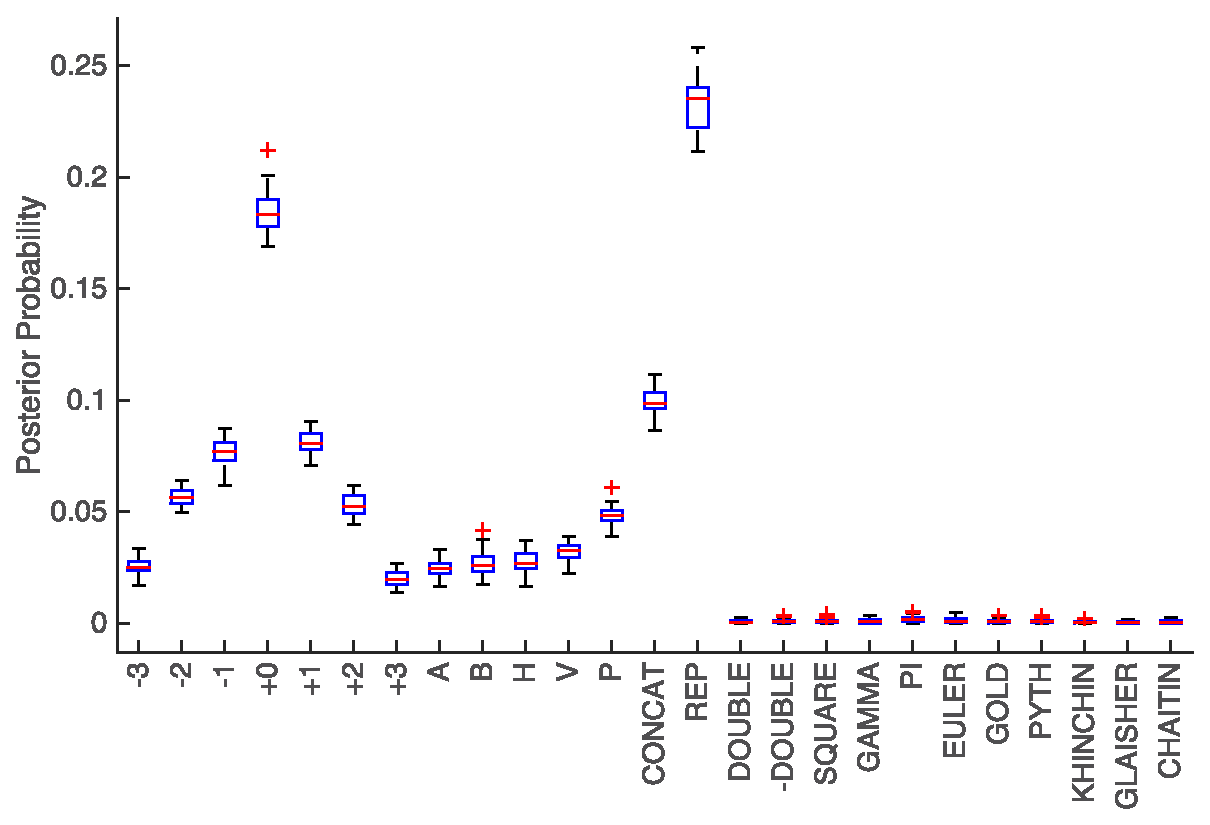
\includegraphics[width=0.8\textwidth]{Fig2}
    %\caption{\bf{Inferred $\theta_i$.} Inferred probability for each production in the grammar}
    \caption{$\theta_i$ inferido. Probabilidad inferida para cada producción de la gramática}
    \label{fig:inferredtheta}
\end{figure}

Aunque 50 pasos puedan parecer pocos para que converja un algoritmo de MCMC, nuestro método calculó $P(p_i \mid d_i, \theta)$ de manera exacta para acelerar la convergencia y para poder luego comparar la probabilidad con la complejidad \mdlgeo del modelo original. En la Figura~\ref{fig:convergetheta}, mostramos una traza de ejemplo para cuatro ejecuciones de MCMC para $\theta_{{\tt +0}}$, que corresponde al valor atómico de la producción \verb#+0#, pero es representativo del comportamiento de todos los $\theta_i$. (consultar la Figura~\ref{S1_Fig} para las trazas del conjunto entero de producciones).

\begin{figure}[htpb]
    \centering
    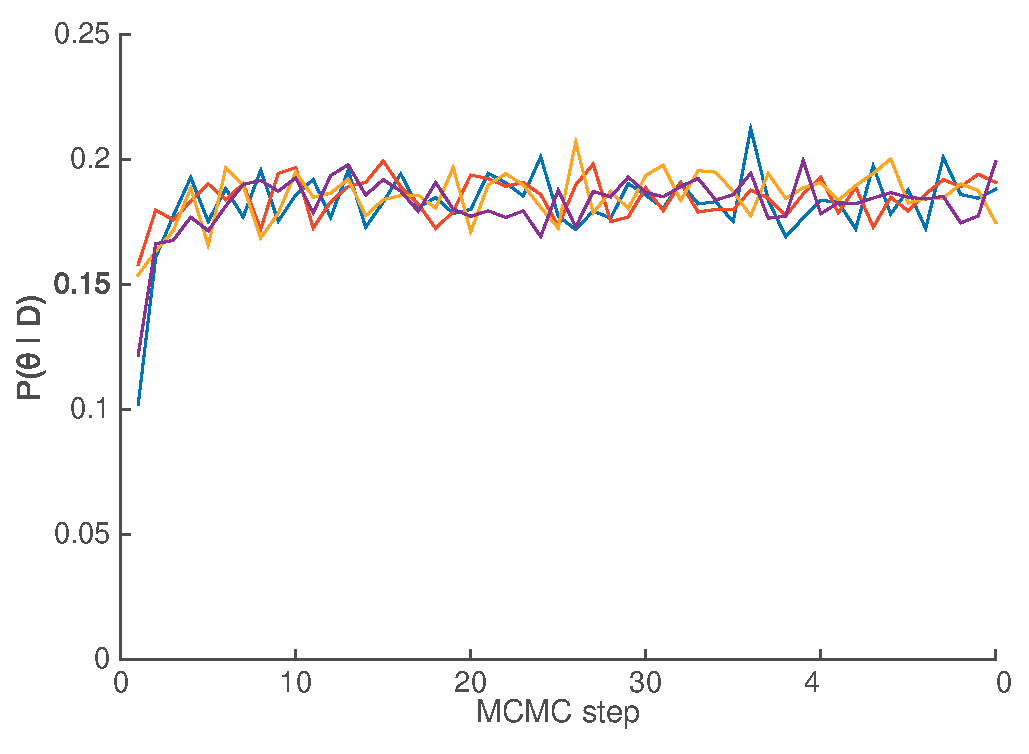
\includegraphics[width=0.8\textwidth]{Fig3}
    %\caption{{\bf Inferred $\theta_{\text{+0}}$.} Inferred probability for +0 production at each step in four MCMC chains.}
    \caption{$\theta_{{\tt +0}}$ inferido. Probabilidad inferida para {\tt +0} en cada paso para cuatro cadenas de MCMC.}
    \label{fig:convergetheta}
\end{figure}
\sergio{La Figura tiene que remplazar CONCAT por la coma: ,}

%Figura~\ref{fig:inferredtheta} shows a remarkable difference between the probability of the productions that were originally used based on geometrical intuitions and the ad-hoc productions. The plot also shows that each clockwise production has almost the same probability as its corresponding anticlockwise production, and a similar relation appears between horizontal and vertical symmetry (H and V) and symmetries around diagonal axes (A and B). This is important because the original experiment was designed to balance such behavior; the inferred grammar reflects this.

La Figura~\ref{fig:inferredtheta} muestra una diferencia notable entre la probabilidad de las producciones que se utilizaron originalmente sobre la base de intuiciones geométricas y las producciones ad-hoc. El gráfico muestra también que cada producción en el sentido horario tiene casi la misma probabilidad que su correspondiente producción en sentido antihorario, y una relación similar aparece entre la simetría horizontal y la vertical (\verb#H# y \verb#V#) y las simetrías alrededor de los ejes diagonales (\verb#A# y \verb#B#). Esto es importante porque el experimento original fue diseñado para equilibrar tal comportamiento y la gramática inferida lo refleja también.

%Figura~\ref{fig:thetaGrouped} shows the same inferred $\theta$ but grouped according to production family. Grouping stresses the low probability of all the ad-hoc productions, but also shows an important difference between REP and the rest of the productions, particularly the simple concatenation of productions (CONCAT). This indicates that the \textit{language of geometry} is capable of reusing simpler structures that capture geometrical meaning to explain the observed data, a key aspect of a successful model of LoT.

La Figura~\ref{fig:thetaGrouped} muestra el mismo $\theta$ inferido pero agrupado según su familia de producción. El agrupamiento destaca la baja probabilidad de todas las producciones ad-hoc, pero también muestra una diferencia importante entre \verb#REP# y el resto de las producciones, particularmente respecto de la simple concatenación de producción (\verb#,#). Esto indica que el lenguaje de geometría es capaz de reutilizar estructuras más simples que captura el significado geométrico para explicar los datos observados, un aspecto clave de un modelo exitoso de \lot que también se ve reflejado en la gramática inferida.

\begin{figure}[!ht]
    \centering
    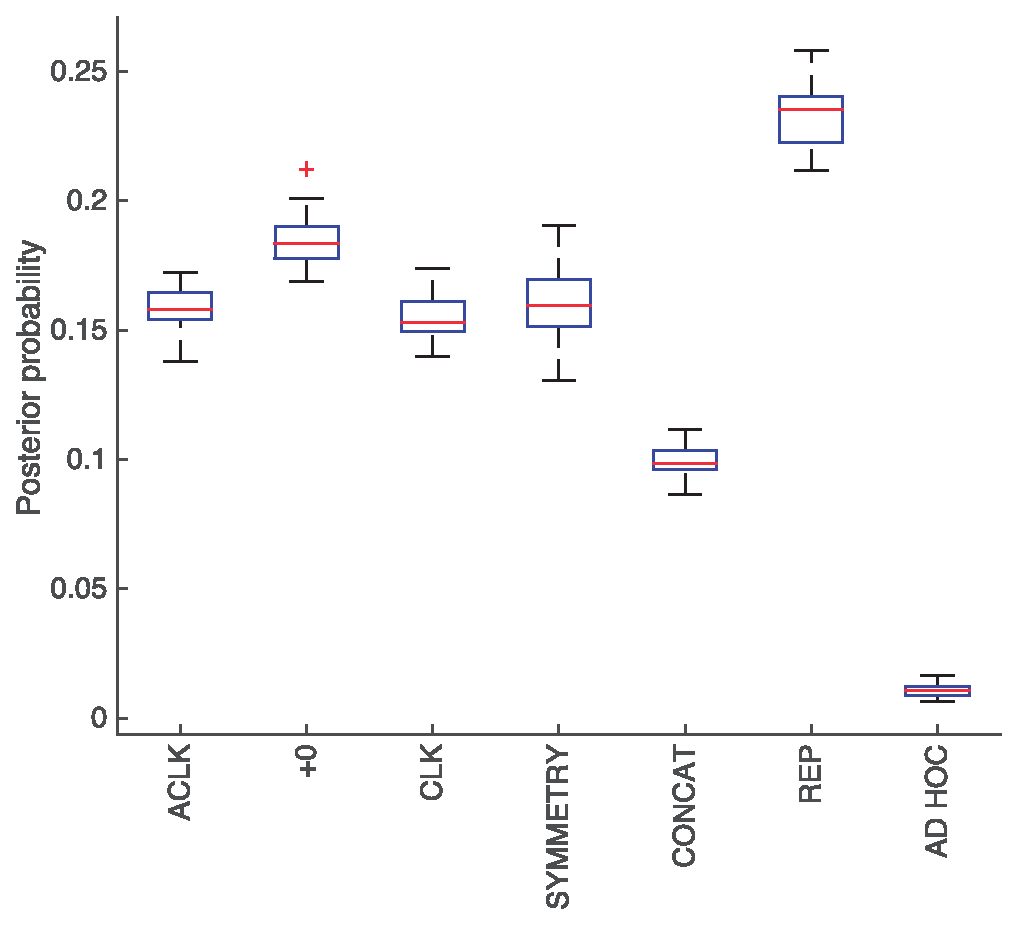
\includegraphics[width=0.8\textwidth]{Fig4}
    \caption{$\theta_i$ inferido agrupado por familia. Probabilidad inferida para cada producción en \gramgeoprima, agrupada por familia.}
    \label{fig:thetaGrouped}
\end{figure}
\sergio{Cambiar CONCAT por la coma en la figura}

%We then ran the same inference method using observed sequences from other experiments but only with the original grammar productions (i.e.\ setting aside the ad-hoc productions). We compared the result of inferring over our previously analyzed sequences generated by adults with sequences generated by children (experiment 2 from ~\cite{amalric2017language}) and the actual expected sequences for an ideal player.

Luego ejecutamos el mismo método de inferencia utilizando las secuencia observadas en otros experimentos, pero sólo con las producciones gramaticales originales (es decir, dejando de lado las producciones ad-hoc). Comparamos el resultado de inferir sobre nuestras secuencias previamente analizadas (que habían sido generadas por adultos) con aquellas generadas por niños (el Experimento 2 de  ~\cite{amalric2017language}) y con las secuencias esperadas para un jugador ideal, es decir, un jugador que siempre elige para cada secuencia $s$ un programa $p$ tal que $\mdlgeo(s) = |p|$ con probabilidad uniforme entre todos los programas mínimos para esa secuencia.

%Figura~\ref{fig:adultVsChildren} shows the probabilities for each atomic production that is inferred after each population. The figure denotes that different populations can converge to different probabilities and thus different LoTs. Specifically, it is worth mentioning that the ideal learner indeed uses more repetition productions than simple concatenations when compared to adults. In the same way, adults use more repetitions than children. This could mean that the ideal learner is capable of reproducing the sequences by recursively embedding other smaller programs, whereas adults and children more so have problems understanding or learning the smaller concept that can explain all the sequences from the experiments, which is consistent with the results from the MDL model in~\cite{amalric2017language}.

La Figura~\ref{fig:adultVsChildren} muestra las probabilidades para cada producción atómica que se infieren de los datos de cada población. La figura denota que diferentes poblaciones pueden converger a diferentes probabilidades y, por tanto, a diferentes LoTs. Específicamente, vale la pena mencionar que el sujeto ideal de hecho utiliza más producciones de repetición que simples concatenaciones en comparación con los adultos. Del mismo modo, los adultos utilizan más repeticiones que los niños. Esto podría significar que el sujeto ideal es capaz de reproducir las secuencias reutilizando de manera recursiva otros programas más cortos, mientras que los adultos y los niños tienen más problemas para comprender o aprender el programa más corto que puede explicar cada una de las secuencias de los experimentos, lo cuál es consistente con los resultados del modelo original de ~\cite{amalric2017language}.

\begin{figure}[!ht]
    \centering
    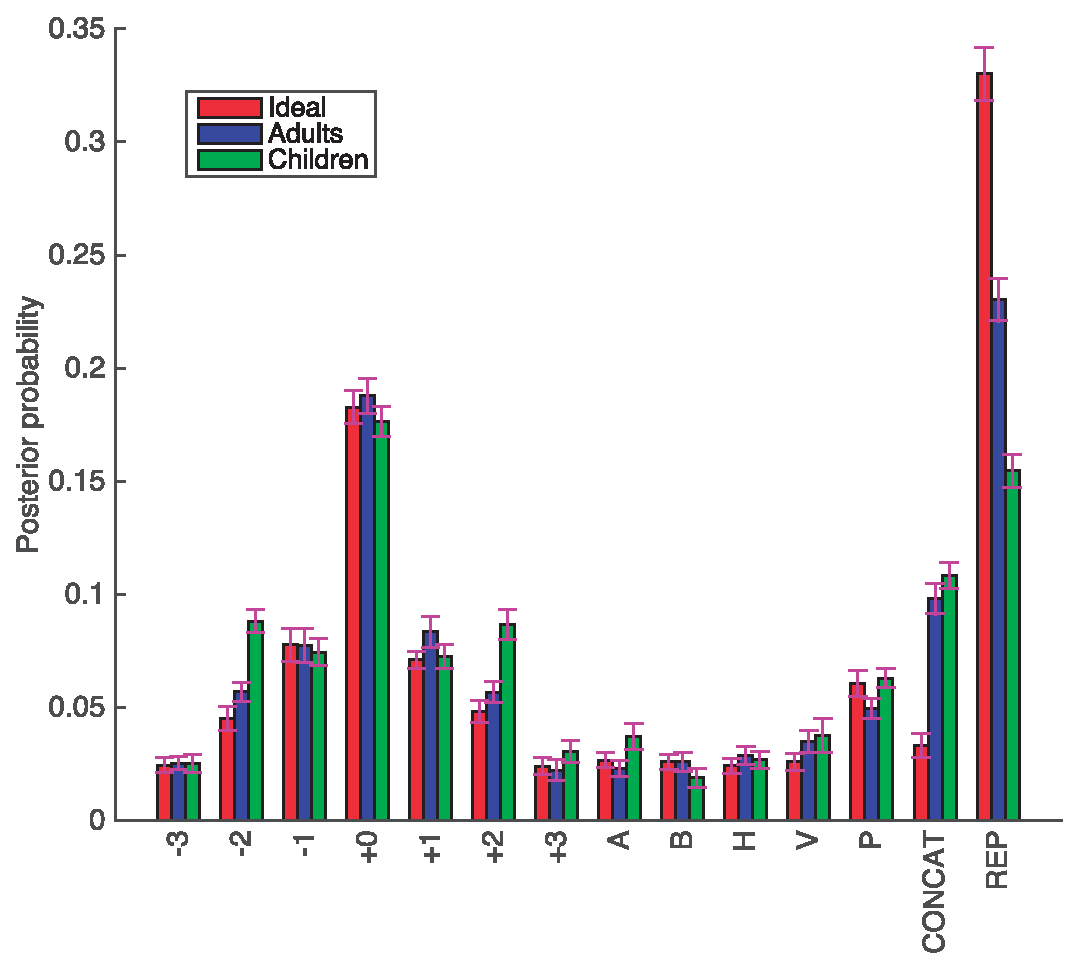
\includegraphics[width=0.8\textwidth]{Fig5}
    %\caption{{\bf Inferred $\theta_i$ for ideal learner, adults and children.} Inferred probability for each production in the grammar for different population data.}
    \caption{$\theta_i$ inferido para el jugador ideal, adultos y niños. Probabilidad inferida para cada producción de \gramgeo para las diferentes poblaciones.}
    \label{fig:adultVsChildren}
\end{figure}
\sergio{Cambiar concat por coma}

%It is worth mentioning that in~\cite{amalric2017language} the complete grammar for the \textit{language of geometry} could explain adults' behavior but had problems to reproduce the children's patterns for some sequences. However, they also showed that penalizing the rotational symmetry (P) could adequately explain children's behavior. In Figura~\ref{fig:adultVsChildren}, we see that the mean value of (P) for children is 0.06 whereas in adults it's 0.05 (a two-sample t-test reveals t = -12.6, p = 10-19). This might not necessarily be contradictory, as the model for children in~\cite{amalric2017language} was used to predict the next symbol of a sequence after seeing its prefix by adding a penalization for extensions that use the rotational symmetry in the {\em minimal} program of each sequence. On the other hand, the Bayesian model in this work tries to explain the observed sequences produced by children considering the probability of a sequence summing over {\em all} the possible programs that can generate it and not just the ones with minimal size. Thus, a production like (P) that might not be part of the minimal program for a sequence might not necessarily be less probable when considering the entire distribution of programs for that same sequence.

Cabe mencionar que en~\cite{amalric2017language} la gramática completa para el \textit{lenguaje de geometría} podía explicar el comportamiento de los adultos, pero tenía problemas para reproducir los patrones de los niños para algunas secuencias. Sin embargo, también demostraron que penalizar a la simetría rotacional (instrucción atómica \verb#P#)  podría explicar adecuadamente el comportamiento de los niños. En la Figura~\ref{fig:adultVsChildren}, vemos que el valor medio de \verb#P# para niños es 0.06 mientras que en adultos es 0.05 (un t-test de dos muestras revela que $t = -12.6, p = 10^{-19}$). Esto puede no ser necesariamente contradictorio, ya que el modelo para niños en~\cite{amalric2017language} fue utilizado para predecir el siguiente símbolo de una secuencia después de ver su prefijo agregando una penalización para extensiones que usan la simetría rotacional \verb#P# \textit{en el programa mínimo} de cada secuencia. Por otro lado, el modelo bayesiano en este trabajo intenta explicar las secuencias observadas producidas por los niños considerando la probabilidad de una secuencia a partir de sumar todos los posibles programas que la pueden generar \textit{y no sólo en los de tamaño mínimo}. Así, una producción como \verb#P# que podría no ser parte del programa mínimo para una secuencia, puede no ser necesariamente menos probable cuando se considera la distribución total de programas para esa misma secuencia.

%\section{Coding Theorem}
\section{Teorema de codificación}
\label{sec:coding}

%For each phenomenon there can always be an extremely large, possibly infinite, number of explanations. In a LoT model, this space is constrained by the grammar $\gram$ that defines the valid hypotheses in the language. Still, one has to define how a hypothesis is chosen among all possibilities. Following Occam's razor, one should choose the simplest hypothesis amongst all the possible ones that explain a phenomenon. In cognitive science, the MDL framework has been widely used to model such bias in human cognition, and in \textit{the language of geometry} in particular~\cite{amalric2017language}. The MDL framework is based on the ideas of information theory~\cite{shannon48}, Kolmogorov complexity~\cite{kolmogorov1968three} and Solomonoff induction~\cite{solomonoff1964formal}.

Para cada fenómeno siempre puede haber un número extremadamente grande, posiblemente infinito, de explicaciones. En un modelo de \lot, este espacio está limitado por la gramática $\gram$ que define las hipótesis válidas en el lenguaje. Aún así, hay que definir cómo se elige una hipótesis entre todas las posibles. Siguiendo el principio de la navaja de Ockham, se debe elegir la hipótesis más simple entre todas las posibles que explican un fenómeno. En ciencia cognitiva, y en \gramgeo en particular, se suele utilizar nociones basadas en el principio de longitud mínima de descripción como \mdlgeo para modelar tal sesgo en la cognición.

%Occam's razor was formalized by Solomonoff~\cite{solomonoff1964formal} in his theory of universal inductive inference, which proposes a universal prediction method that successfully approximates any distribution $\mu$ based on previous observations, with the only assumption of $\mu$ being computable. In short, Solomonoff's theory uses all programs (in the form of prefix Turing machines) that can describe previous observations of a sequence to calculate the probability of the next symbols in an optimal fashion, giving more weight to shorter programs. Intuitively, simpler theories with low complexity have higher probability than theories with higher complexity. Formally, this relationship is described by the Coding Theorem~\cite{levin1974laws}, which closes the gap between the concepts of Kolmogorov complexity and probability theory. However, LoT models that define a probabilistic distribution for their hypotheses do not attempt to compare it with a complexity measure of the hypotheses like the ones used in MDL, nor the other way around.

El principio de la navaja de Ockham fue formalizado por Solomonoff~\cite{solomonoff1964formal} en su teoría universal de la inferencia inductiva, que propone un método de predicción universal que aproxima cualquier distribución $\mu$ a partir de observaciones previas, con el único supuesto de que $\mu$ sea computable. En resumen, la teoría de Solomonoff utiliza todos los programas (en la forma de máquinas de Turing libres de prefijos) que pueden describir las observaciones previas de una secuencia para calcular la probabilidad de los siguientes símbolos de una manera óptima, dando más peso a los programas más cortos. Intuitivamente, las teorías más simples, con baja complejidad, tienen mayor probabilidad que las teorías de mayor complejidad. Formalmente, esta relación es descrita en el Teorema de codificación~\cite{levin1974laws}, que cierra la brecha entre los conceptos de complejidad de Kolmogorov y la teoría de probabilidad. Sin embargo, los modelos de \lot que definen una distribución probabilística para sus hipótesis no han intentado compararla con una medida de complejidad de las hipótesis como las que se usan en \mdlgeo, ni al revés.

%In what follows we formalize the Coding Theorem (for more information, see~\cite{li2013introduction}) and test it experimentally. To the best our knowledge, this is the first attempt to validate these ideas for a particular (non universal) language. The reader should note that we are not validating the theorem itself as it has already been proved for universal Turing Machines. Here, we are testing whether the inverse logarithmic relationship between the probability and complexity holds true when defined for a specific non universal language.

A continuación, formalizamos el Teorema de Codificación (para obtener más información, consulte~\cite{li2013introduction}) y lo probamos experimentalmente. Hasta donde sabemos, este es el primer intento para validad estas ideas para un lenguaje particular (no universal). El lector debe tener en cuenta que no estamos validando el teorema en sí, dado que ya ha sido probado para Máquinas de Turing universales. Aquí estamos probando si la relación logarítmica inversa entre la probabilidad y la complejidad podría mantenerse cuando se definen para un lenguaje específico no universal.

%\subsection{The formal statement}
\subsection{La definición formal}

%Let $M$ be a prefix Turing machine --by {\em prefix} we mean that if $M(x)$ is defined, then $M$ is undefined for every proper extension of $x$. Let $P_M(x)$ be the probability that the machine $M$ computes output $x$ when the input is filled-up with the results of fair coin tosses, and let $K_M(x)$ be the {\em Kolmogorov complexity of $x$ relative to $M$}, which is defined as the length of the shortest program which outputs $x$, when executed on $M$. The Coding Theorem states that for every string $x$ we have

\widesanti{La parte de TM libre de prefijos y K ya va a haber sido presentada en la intro}
\widesergio{Definir desde donde y desde donde no de la intro finalmente}
Sea $M$ una Máquina de Turing libre de prefijos --por {\em libre de prefijo} nos referimos a que si $M(x)$ está definida, entonces $M$ está indefinida para cualquier extensión de $x$. Sea $P_M(x)$ la probabilidad de que la máquina $M$ compute la salida $x$ cuando la entrada se llena con los resultados de los lanzamientos de una moneda justa, y sea $K_M(x)$ la {\em complejidad de Kolmogorov de $x$ relativa a $M$}, que se define como la longitud del programa más corto que genera $x$, cuando se ejecuta en $M$. El Teorema de Codificación establece que, por cada cadena $x$ tenemos:
%
\begin{equation*}
\label{eqF}
\log \frac{1}{P_U(x)} = K_U(x)
\end{equation*}
%
%up to an additive constant, whenever $U$ is a {\em universal} prefix Turing machine --by {\em universal} we mean a machine which is capable of simulating every other Turing machine; it can be understood as the underlying (Turing-complete) chosen programming language. It is important to remark that neither $P_U$, nor $K_U$ are computable, which means that such mappings cannot be obtained through effective means. However, for specific (non-universal) machines $M$, one can, indeed, compute both $P_M$ and $K_M$.
salvo una constante aditiva, siempre que $U$ sea una Máquina Universal de Turing libre prefijos --por {\em Universal} nos referimos a una máquina que es capaz de simular cualquier otra máquina de Turing; puede entenderse como el lenguaje de programación elegido subyacente (Turing-completo). Es importante señalar que ni $P_U$, ni $K_U$ son computables, lo que significa que tal mapeo no puede obtenerse por medios efectivos. Sin embargo, para máquinas específicas (no universales) $M$, uno puede, de hecho, calcular tanto $P_M$ como $K_M$.

%\subsection{Testing the Coding Theorem for \boldmath{$\gramgeo$}}
\subsection{Revisando el teorema de codificación para $\gramgeo$}

%Despite the fact that $P_M$ and $K_M$ are defined over a Turing Machine $M$, the reader should note that a LoT is not usually formalized with a Turing Machine, but instead as a programming language with its own syntax of valid programs and semantics of execution, which stipulates how to compute a concept from a program. However, one can understand programming languages as defining an equivalent (not necessarily universal) Turing Machine model, and a LoT as defining its equivalent (not necessarily universal) Turing Machine $\gram$. In short, machines and languages are interchangeable in this context: they both specify the programs/terms, which are symbolic objects that, in turn, describe semantic objects, namely, strings.

A pesar de que $P_M$ y $K_M$ están definidos sobre una máquina de Turing $M$, el lector debe tener en cuenta que un \lot no se suele formalizar con una máquina de Turing, sino como un lenguaje de programación con su propia sintaxis de programas válidos y su propia semántica de ejecución que estipula cómo calcular un concepto a partir de un programa válido. Sin embargo, uno puede concebir los lenguajes de programación como la definición de una máquina de Turing equivalente (no necesariamente universal), y a un \lot como un lenguaje que define a su equivalente máquina de Turing (no necesariamente universal), En resumen, las máquinas y los lenguajes son intercambiables en este  sentido: ambas especifican los programas/términos, los cuales son objetos simbólicos que, a su vez, describen objetos semánticos (a saber, cadenas). Para \gramgeo ya tenemos definida su medida de $K_M$ a la cual hemos notado \mdlgeo, a continuación definiremos $P_M$ para el mismo lenguaje.

%\paragraph{The Kolmogorov complexity relative to \boldmath{$\gramgeo$}}

%In~\cite{amalric2017language}, the Minimal Description Length was used to model the combination of productions from the \textit{language of geometry} into concepts by defining a Kolmogorov complexity relative to the {\em language of geometry}, which we denote $\mdlgeo$. $\mdlgeo(x)$ is the minimal size of an expression in the grammar of $\gramgeo$ which describes $x$. The formal definition of `size' can be found in the cited work but in short: each of the atomic productions adds a fixed cost of $2$ units; using any of the repetition productions to iterate $n$ times a list of other productions adds the cost of the list, plus $\lfloor \log(n) \rfloor$; and joining two lists with a concatenation costs the same as the sum of the costs of both lists.


%\paragraph{The probability relative to \boldmath{$\gramgeo$}} On the other hand, with the Bayesian model specified in this work, we can define $P(x \mid \gramgeo, \theta)$ which is the probability of a string $x$ relative to $\gramgeo$ and its vector of probabilities for each of the productions.

\paragraph{La probabilidad relativa $\gramgeo$.} 

Con el modelo Bayesiano especificado en este capítulo podemos definir $P(x \mid \gramgeo, \theta)$ que es la probabilidad de una cadena $x$ relativa a $\gramgeo$ y el vector de probabilidades para cada una de las producciones.

%For the sake of simplicity, we will use $P_{\gramgeo}(x)$ to denote $P(x \mid \gramgeo, \theta)$ when $\theta$ is the inferred probability from the observed adult sequences from the experiment.
En aras de la simplicidad, usaremos $P_{\gramgeo}(x)$ para denotar $P(x \mid \gramgeo, \theta)$ cuando $\theta$ es la probabilidad inferida de las secuencias de adultos observadas en el experimento.
%
\begin{eqnarray*}
\label{eqG}
P_{\gramgeo}(x) &=& P(x \mid \gramgeo, \theta)\\
&=& \sum_{\prog} P(x \mid \prog, \theta)\\
&\propto &\sum_{\prog} P(x \mid \prog) P(\prog \mid \theta).
\end{eqnarray*}
%

%Here, we calculate both $P_{\gramgeo}(x)$ and $K_{\gramgeo(x)}$ in an exact way (note that $\gramgeo$, seen as a programming language, is not Turing-complete). In this section, we show an experimental equivalence between such measures which is consistent with the Coding Theorem. We should stress, once more, that the theorem does not predict that this relationship should hold for a specific non-universal Turing Machine.

Aquí, calculamos tanto $P_{\gramgeo}(x)$ como $\mdlgeo(x)$ de una manera efectiva (tener en cuenta que $\gramgeo$, visto como un lenguaje de programación, no es Turing-completo). En esta sección, mostramos un experimento de equivalencia entre tales medidas que es consistente con el Teorema de Codificación. Queremos enfatizar, una vez más, que el teorema no predice que esta relación deba mantenerse para una máquina de Turing específica no universal.


%To calculate $P_{\gramgeo}(x)$ we are not interested in the normalization factor of $P(x \mid \prog) P(\prog \mid \theta)$ because we are just trying to measure the relationship between $P_{\gramgeo}$ and $\mdlgeo$ in terms of the Coding Theorem. Note, however, that calculating $P_{\gramgeo}(x)$ involves calculating all programs that compute each of the sequences as in our previous experiment. To make this tractable we calculated $P_{\gramgeo}(x)$ for 10,000 unique random sequences for each of the possible sequence lengths from the experiment (i.e., up to eight). When the length of the sequence did not allow 10,000 unique combinations, we used all the possible sequences of that length.

Para calcular $P_{\gramgeo}(x)$ no nos interesa el factor de normalización de $P(x \mid \prog) P(\prog \mid \theta)$ porque sólo estamos tratando de medir la relación entre $P_{\gramgeo}$ y $\mdlgeo$ en términos del Teorema de Codificación. Sin embargo, hay que tener en cuenta que el cálculo de $P_{\gramgeo}(x)$ implica calcular todos los programas que computan cada una de las secuencias como en nuestro experimento anterior. Para hacer esto tratable, calculamos $P_{\gramgeo}(x)$ para 10.000 secuencias aleatorias únicas para cada una de las posibles longitudes de las secuencias del experimento (es decir, hasta ocho). Cuando la longitud de la secuencia no permitió 10.000 combinaciones únicas, utilizamos todas las posibles secuencias de esa longitud.

%\subsection{Coding Theorem Results}
\subsection{Resultados del Teorema de Codificación}

%Figura~\ref{fig:codR} shows the mean probability $P_{\gramgeo}(x)$ for all sequences $x$ with the same value of $K_{\gramgeo(x)}$ and length between 4 and 8 ($|x| \in \left[4,8 \right]$) for all generated sequences $x$. The data is plotted with a logarithmic scale for the x-axis, illustrating the inverse logarithmic relationship between $\mdlgeo(x)$ and $P_{\gramgeo}(x)$. The fit is very good, with $R^2=.99$, $R^2=.94$, $R^2=.97$, $R^2=.99$ and $R^2=.98$ for Figura~\ref{fig:codR}A, Figura~\ref{fig:codR}B, Figura~\ref{fig:codR}C, Figura~\ref{fig:codR}D and Figura~\ref{fig:codR}E, respectively.

La Figura~\ref{fig:codR} muestra la probabilidad media $P_{\gramgeo}(x)$ para todas las secuencias $x$ con el mismo valor de $\mdlgeo(x)$ y una longitud entre 4 y 8 ($|x| \in \left[4,8 \right]$) para todas las secuencias generadas $x$. Los datos se trazan con una escala logarítmica para el eje x, ilustrando la relación logarítmica inversa entre $\mdlgeo(x)$ y $P_{\gramgeo}(x)$. El ajuste es muy bueno, con $R^2=.99$, $R^2=.94$, $R^2=.97$, $R^2=.99$ y $R^2=.98$ para Figura~\ref{fig:codR}A, Figura~\ref{fig:codR}B, Figura~\ref{fig:codR}C, Figura~\ref{fig:codR}D y Figura~\ref{fig:codR}E, respectivamente.

\begin{figure}[!ht]
    \centering
    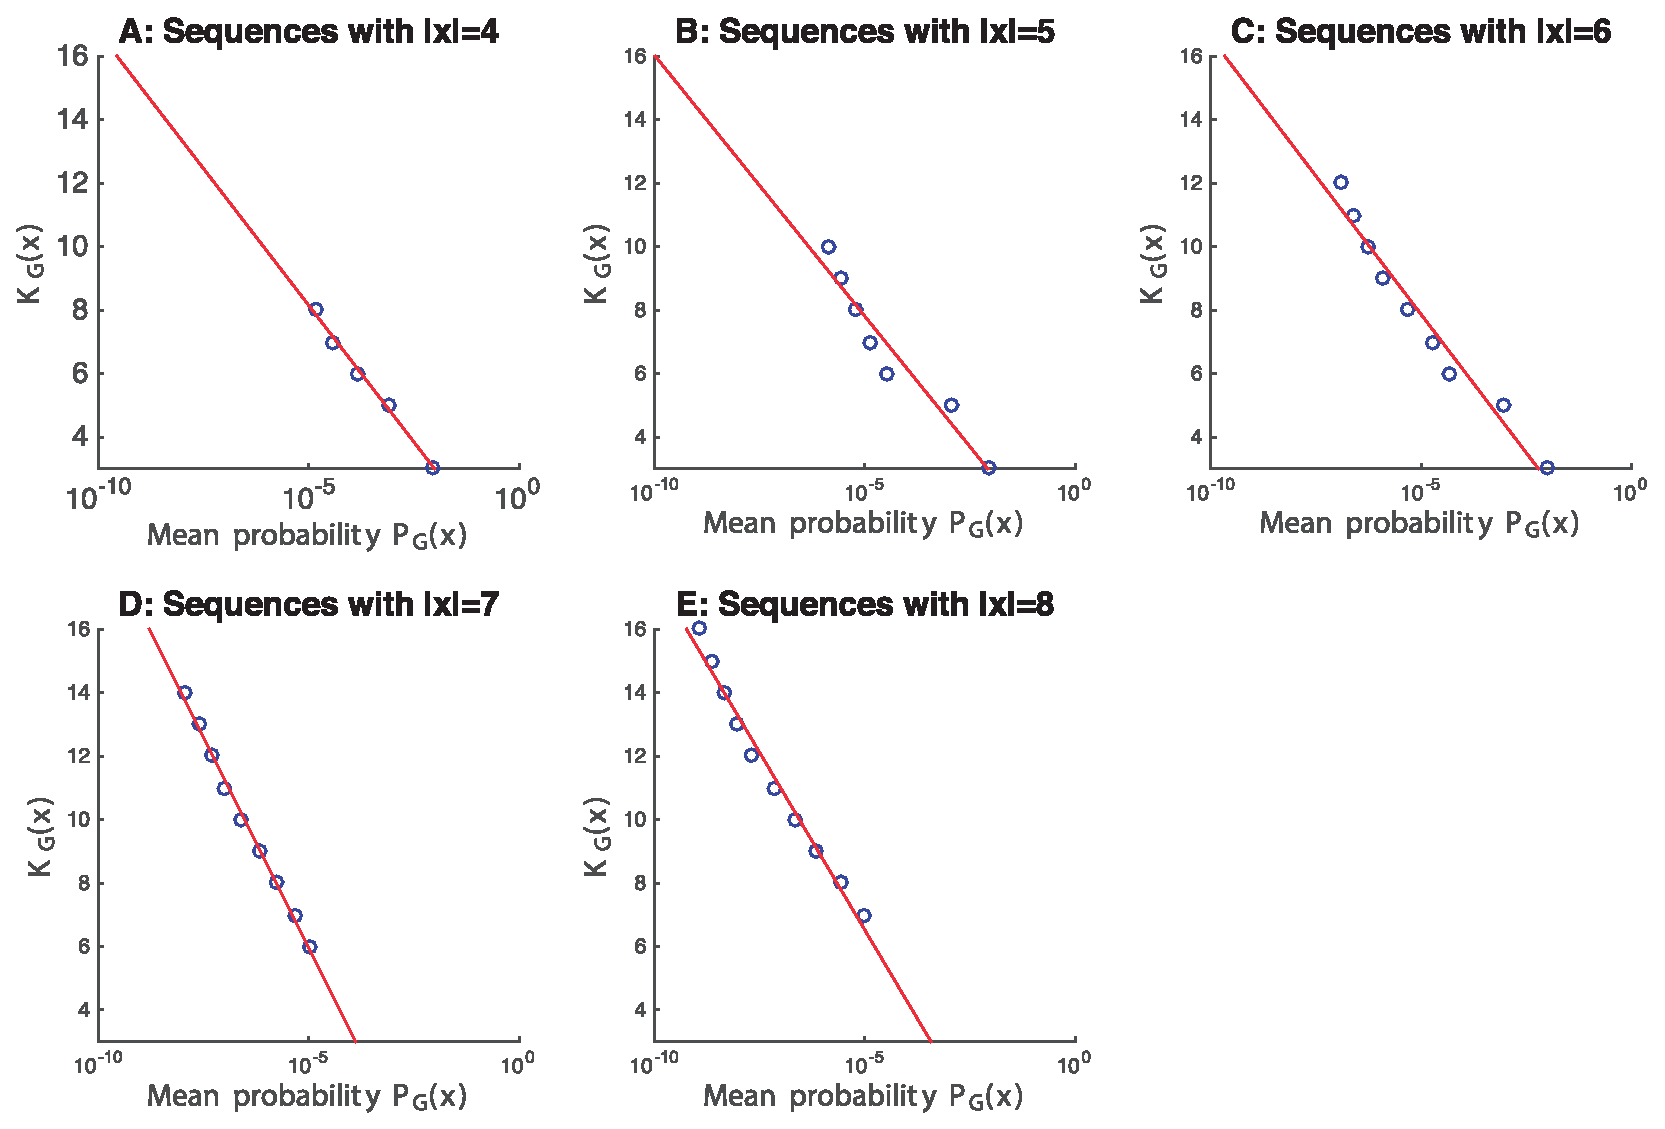
\includegraphics[width=0.8\textwidth]{Fig6}
    \caption{Probabilidad media $P_{\gramgeo}(x)$ para todas las secuencias $x$ con el mismo valor de $\mdlgeo(x)$.
    Subfigura A: secuencias con $|x| = 4$.
    Subfigura B: secuencias con $|x| = 5$.
    Subfigura C: secuencias con $|x| = 6$.
    Subfigura D: secuencias con $|x| = 7$.
    Subfigura E: secuencias con $|x| = 8$.}
    \label{fig:codR}
\end{figure}

%This relationship between the complexity $\mdlgeo$ and the probability $P_{\gramgeo}$ defined for finite sequences in the \textit{language of geometry}, matches the theoretical prediction for infinite sequences in universal languages described in the Coding Theorem. At the same time, it captures the Occam's razor intuition that the simpler sequences one can produce or explain with this language are also the more probable.

Esta relación entre la complejidad $\mdlgeo$ y la probabilidad $P_{\gramgeo}$ definidas para secuencias finitas en \gramgeo, coincide con al predicción teórica para cadenas en lenguajes universales descrita en el Teorema de Codificación. Al mismo tiempo, captura la intuición de la navaja de Ockham por la cual las secuencias más simples que uno puede producir o explicar en este lenguaje son también las más probables.

%Figura~\ref{fig:codK:8} and Figura~\ref{fig:codP:8} show the histogram of $P_{\gramgeo}(x)$ and $\mdlgeo(x)$, respectively, for sequences with length = 8 to get a better insight about both measures. The histogram of the rest of the sequence's lengths are included in \nameref{S2_Fig} and \nameref{S3_Fig} for completeness, and they all show the same behavior.

En Figura~\ref{fig:codK:8} y Figura~\ref{fig:codP:8} se muestra el histograma de $P_{\gramgeo}(x)$ y $\mdlgeo(x)$, respectivamente, para secuencias de longitud = 8 para obtener una mejor idea de ambas distribuciones. El histograma del resto de las longitudes de la secuencia se incluyen en las Figuras \ref{S2_Fig} y \ref{S3_Fig} por completitud, y todos muestran el mismo comportamiento.

\begin{figure}[!ht]
    \centering
    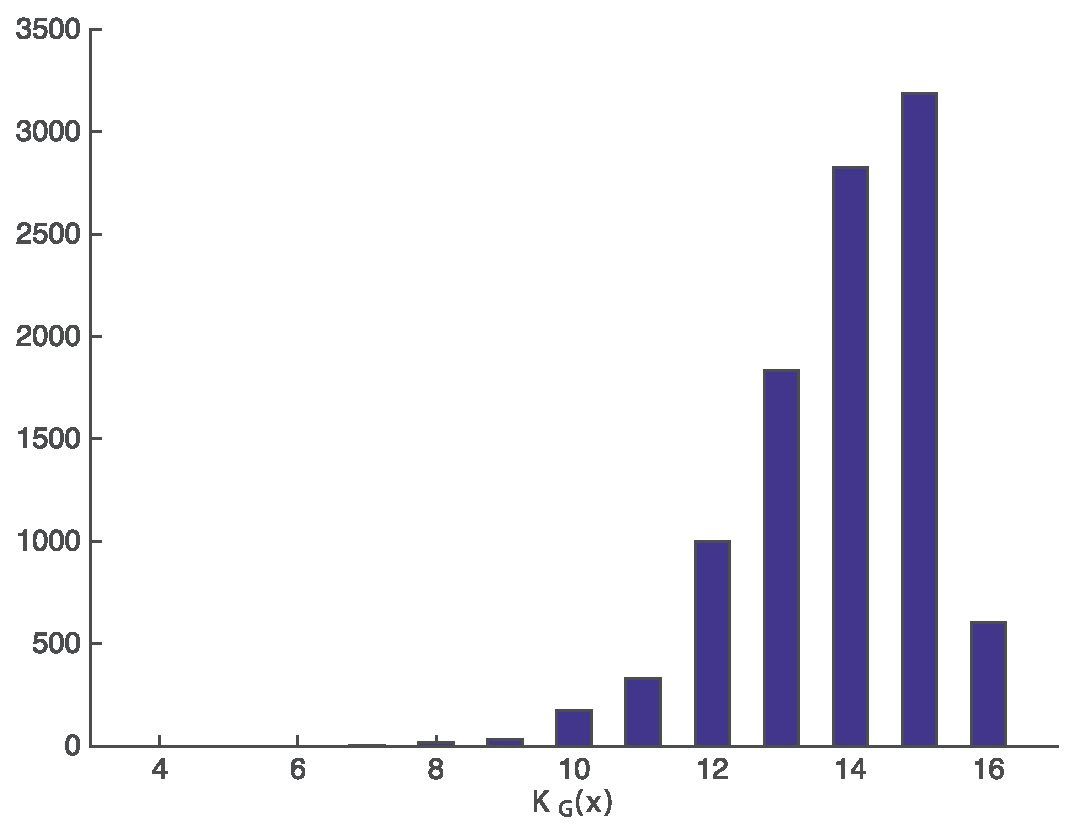
\includegraphics[width=0.8\textwidth]{Fig7}
    %\caption{{\bf Histogram of complexity $\mdlgeo(x)$.} Histogram of complexity for sequences $x$ with $|x| = 8$.}
    \caption{Histograma de complejidad $\mdlgeo(x)$ para secuencias $x$ con $|x| = 8$.}
    \label{fig:codK:8}
\end{figure}


\begin{figure}[!ht]
    \centering
    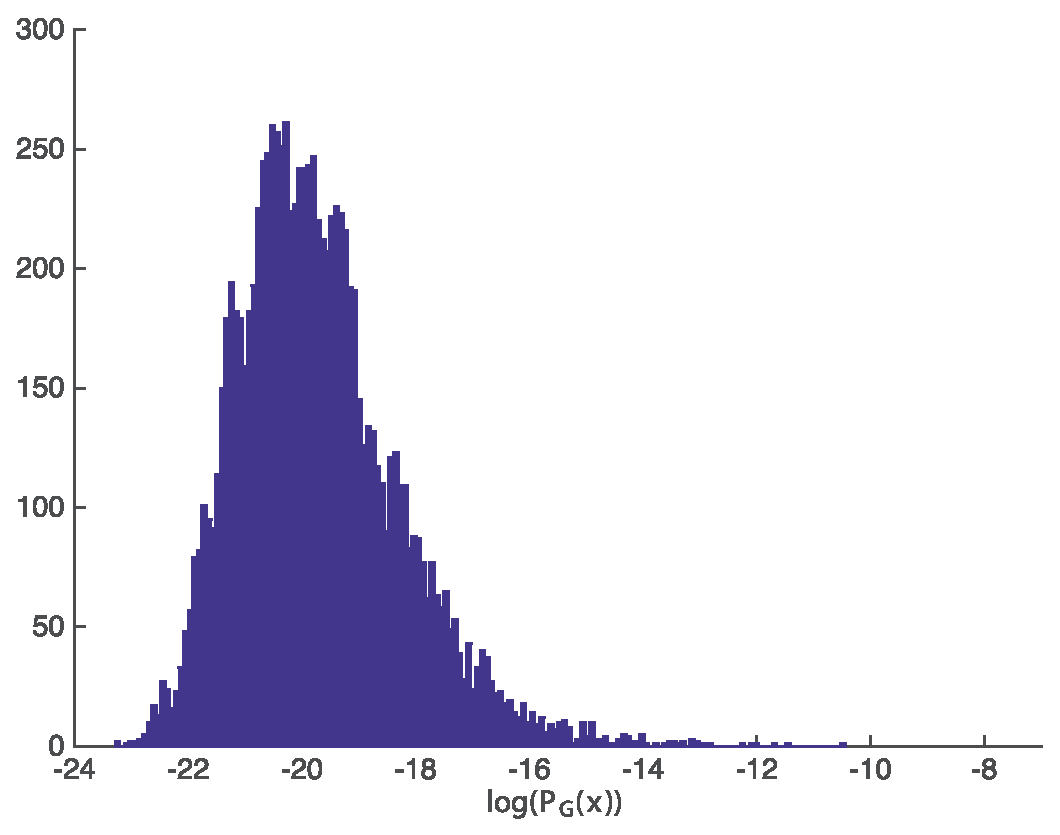
\includegraphics[width=0.8\textwidth]{Fig8}
    %\caption{{\bf Histogram of probability $P_{\gramgeo}(x)$.} Histogram of probability for sequences $x$ with $|x| = 8$.}
    \caption{Histograma de probabilidad $P_{\gramgeo}(x)$ para secuencias $x$ con $|x| = 8$.}
    \label{fig:codP:8}
\end{figure}

%\section{Discussion}
\section{Discusión}

%We have presented a Bayesian inference method to select the set of productions for a LoT and test its effectiveness in the domain of a geometrical cognition task. We have shown that this method is useful to distinguish between arbitrary ad-hoc productions and productions that were intuitively selected to mimic human abilities in such domain.

Hemos presentado un método de inferencia bayesiano para seleccionar el conjunto de producciones para un \lot y probado su eficacia en el dominio de una tarea de cognición geométrica. Mostramos que este método es útil para distinguir entre producciones ad-hoc arbitrarias y producciones que fueron seleccionadas intuitivamente para imitar las habilidades humanas en ese dominio.

%The proposal to use Bayesian models tied to PCFG grammars in a LoT is not new. However, previous work has not used the inferred probabilities to gain more insight about the grammar definition in order to modify it. Instead, it had usually integrated out the production probabilities to better predict the data, and even found that hierarchical priors for grammar productions show no significant differences in prediction results over uniform priors~\cite{piantadosi2012bootstrapping,yildirim2015learning}.

La propuesta de utilizar modelos bayesianos vinculados a gramáticas PCFG en un \lot no es nueva. Sin embargo, los trabajos anteriores no han utilizado las probabilidades inferidas para obtener más información sobre la definición de la gramática y modificarla. En cambio, han integrado usualmente las probabilidades de producción para predecir mejor los datos e incluso se mostró que el uso de distribuciones a priori jerárquicas para las producciones gramaticales no muestran diferencias significativas en los resultados de predicción sobre el uso de distribuciones a priori uniformes~\cite{piantadosi2012bootstrapping,yildirim2015learning}.

%We believe that inferring production probabilities can help prove the adequacy of the grammar, and can further lead to a formal mechanism for selecting the correct set of productions when it is not clear what a proper set should be. Researchers could use a much broader set of productions than what might seem intuitive or relevant for the domain and let the hierarchical Bayesian inference framework select the best subset.

Creemos que inferir probabilidades de producción puede ayudar a demostrar la adecuación de una gramática para un dominio, y puede conducir a un mecanismo formal para seleccionar el conjunto correcto de producciones cuando no está claro cuál debería ser el conjunto correcto. Los investigadores podrían utilizar un conjunto de producciones más amplios que aquellas que parezcan intuitivas o relevantes para el dominio y dejar que la inferencia bayesiana seleccione el mejor subconjunto.

%Selecting a broader set of productions still leaves some arbitrary decisions to be made. However, it can help to build a more robust methodology that --combined with other ideas like testing grammars with different productions for the same task~\cite{piantadosi2016logical}-- could provide more evidence of the adequacy of the proposed LoT.

La selección de un conjunto más amplio de producciones todavía deja algunas decisiones arbitrarias por tomar. Sin embargo, puede contribuir a construir una metodología más sólida que --combinada con otras ideas como probar gramáticas con diferentes producciones para la misma tarea~\cite{piantadosi2016logical}-- podría proporcionar más evidencia de la idoneidad del \lot propuesto.

%Having a principled method for defining grammars in LoTs is a crucial aspect for their success because slightly different grammars can lead to different results, as has been shown in~\cite{piantadosi2016logical}.

Tener un método basado en principios para definir gramáticas en \lot es un aspecto crucial para su éxito, porque gramáticas ligeramente diferentes pueden conducir a resultados muy diversos como se ha demostrado en~\cite{piantadosi2016logical}.

%The experimental data used in this work was designed at~\cite{amalric2017language} to understand how humans encode visuo-spatial sequences as structured expressions. As future research, we plan to perform a specific experiment to test these ideas in a broader range of domains. Additionally, data from more domains is needed to demonstrate if this method could also be used to effectively prove whether different people use different LoT productions as outlined in Figura~\ref{fig:adultVsChildren}.

Los datos experimentales utilizados en este trabajo fueron diseñados en~\cite{amalric2017language} para comprender cómo los humanos codifican secuencias visuoespaciales como expresiones estructuradas. Como investigaciones futuras, podrían realizarse experimentos específicos para probar estas ideas en un rango de dominios más amplios. Además, se necesitan aún más experimentos para probar la efectividad del método y ver si permite individualizar las diferencias de las producciones de los LoTs para distintas poblaciones, como se describió en la Figura~\ref{fig:adultVsChildren}.

%Finally, we showed an empirical equivalence between the complexity of a sequence in a minimal description length (MDL) model and the probability of the same sequence in a Bayesian inference model which is consistent with the theoretical relationship described in the Coding Theorem. This opens an opportunity to bridge the gap between these two approaches that had been described ad complementary by some authors~\cite{mackay2003information}.

Finalmente, mostramos una equivalencia empírica entre la complejidad de una secuencia en un modelo de longitud de descripción mínima y la probabilidad de la misma secuencia en un modelo de inferencia bayesiano, lo cual es consistente con la relación teórica descrita en el Teorema de Codificación. Esto abre una oportunidad para cerrar la brecha entre estos dos enfoques que han sido descritos como complementarios por algunos autores~\cite{mackay2003information}.


    %!TEX root = ../main.tex

%\begin{abstract}
%Recent approaches to human concept learning have successfully combined the power of symbolic, infinitely productive rule systems and statistical learning to explain our ability to learn new concepts from  just a few examples. The aim of most of these studies is to reveal the underlying language structuring these representations and providing a general substrate for thought. However, describing a model of thought that is fixed once trained is against the extensive literature that shows how experience shapes concept learning. Here, we ask about the plasticity of these symbolic descriptive languages. We perform a concept learning experiment that demonstrates that humans can change very rapidly the repertoire of symbols they use to identify concepts, by compiling expressions which are frequently used into new symbols of the language. The pattern of concept learning times is accurately described by a Bayesian agent that rationally updates the probability of compiling a new expression according to how useful it has been to compress concepts so far. By portraying the Language of Thought as a flexible system of rules, we also highlight the difficulties to pin it down empirically.
%\end{abstract}

%\chapter{BORRAR: Towards a more flexible Language of Thought: Bayesian grammar updates after each concept exposure}
\chapter{Hacia un lenguaje del pensamiento más flexible: Actualizaciones bayesianas de la gramática tras la exposición a cada concepto}\label{chapter:PRE}
\chaptermark{Actualizaciones bayesianas tras exposiciones}

\section{Introducción}




%In the domain of Boolean concepts, a wide range of logical varieties of concepts was studied in~\cite{feldman2003simplicity}, revealing a surprisingly simple `law': the subjective difficulty of a Boolean concept for a human learner is directly proportional to the length of the shortest compatible program in the language of propositional logic (i.e.\ Boolean variables combined with the operators \textit{and}, \textit{or} and \textit{not}). This result may suggest that human \lot is equipped with rules and symbols similar to those found in propositional logic. Indeed, the correlation between the subjective difficulty of concepts and their complexity has been used as a general vehicle to study human \lot in various domains~\cite{piantadosi2016logical,leeuwenberg1971perceptual,amalric2017language,romano2018,lupyan2007language}. Although often implicit, the general strategy is to (\textit{1)} assume a language; (\textit{2)} find the shortest compatible program for some concepts in that language; (\textit{3)} compare the length of these programs with the subjective difficulty of the concepts; and finally (\textit{4)} repeat this process for various languages within a universe of possible candidates and choose the language that gives the best match in \textit{(3)}. As mentioned before, the length of the program depends on the primitives of the language in which this program is written, so different languages make different predictions.

Como hemos visto en los capítulos anteriores, un lenguaje que describe conceptos también proporciona una noción natural de su complejidad. En el dominio de los conceptos booleanos, se ha estudiado una amplia variedad de conceptos lógicos~\cite{feldman2003simplicity}, revelando una `ley' sorprendentemente simple: la dificultad subjetiva de aprender un concepto booleano para un humano es directamente proporcional a la longitud del programa compatible más corto en el lenguaje de la lógica proposicional (es decir, un lenguaje con símbolos para variables booleanas que pueden combinarse con los operadores de \textit{conjunción}, \textit{disyunción} y \textit{negación}). Este resultado puede sugerir que el \lot está equipado con reglas y símbolos similares a los que se encuentran en la lógica proposicional.

%A natural question, however, is whether the primitives of a \lot are universal --both across different individuals and also throughout development-- or if instead the semantic repertoire of a language is dynamic and shaped by experience. Indeed, it is likely that our ability to automatically represent Boolean concepts in a succinct manner is not due to an innate efficient propositional language in our mind. Instead, we propose that this ability arises as a byproduct of our brain rapidly learning efficient representations for the concepts we usually  encounter in everyday life. Our research question is: how rapidly can we adapt our learning mechanisms when we encounter a new domain in which our a priori representations are no longer efficient? We examine the hypothesis that humans have the ability to rapidly recombine propositions in their \lot, adding new primitives to their language. In other words, that learning leads to a process of compiling routines into functions within the \lot.

En el Capítulo~\ref{chapter:PO} presentamos un mecanismo de validación adicional para robustecer el proceso de selección de un \lot. Sin embargo, una pregunta natural es si las primitivas de un \lot son universales, tanto a través de diferentes individuos como también a lo largo del desarrollo. O si en cambio, el repertorio de símbolos de un lenguaje es dinámico y está moldeado por la experiencia. De hecho, es probable que nuestra capacidad para representar automáticamente conceptos booleanos de una manera sucinta no se deba a un lenguaje proposicional eficiente innato en nuestra mente. En cambio, es probable que esta habilidad surja como un subproducto del hecho de que nuestro cerebro aprende rápidamente representaciones eficientes para los conceptos que solemos encontrar en la vida cotidiana. La pregunta que guía este capítulo es: ¿qué tan rápido podemos adaptar nuestros mecanismos de aprendizaje cuando nos encontramos con un nuevo dominio en el que nuestras representaciones a priori ya no son eficientes? Examinamos la hipótesis de que los humanos tienen la capacidad de recombinar rápidamente proposiciones en su \lot, agregando nuevas primitivas al lenguaje. En otras palabras, que el aprendizaje conduce a un proceso de compilación de rutinas en nuevos símbolos de funciones dentro del \lot.

%In the example of the Logo language one can imagine that if productions which draw squares are very frequent, it would be efficient to devote a new symbol to this production. The new symbol `square' is a hierarchical `second order' construction of the `first order' primitives of the language. It has a cost (of increasing the lexicon of the language) but in the new language, drawing a square can be instantiated with a very short program (namely, `square') and hence uses less memory. Indeed, a higher level language allows us to reach a higher level of abstraction by freeing memory and processing power, thus making more complex thoughts thinkable~\cite{minsky1967computation,murphy1988comprehending}.

%Por ejemplo, si uno utiliza un lenguaje similar al Logo~\cite{abelson1974logo} para describir figuras, tiene a su disposición símbolos de producciones básicas como `mover', `lápiz arriba', `lápiz abajo' o `rotar' para generar un conjunto infinito de programas que, cuando se evalúan, pueden trasmitir diversas formas. Si los programas que dibujan cuadrados son muy frecuentes, entonces sería conveniente dedicar un nuevo símbolo a esta producción. El nuevo símbolo `cuadrado' es una construcción jerárquica de {\em segundo orden} construido a partir de las primitivas de {\em primer orden} del lenguaje. Incrementar los símbolos del lenguaje tiene un costo, pero en el nuevo lenguaje, dibujar un cuadrado puede ser instrumentado con un programa muy corto (simplemente, `cuadrado') y, por tanto, utilizando menos memoria. De esta manera, un lenguaje de nivel superior nos permite alcanzar un mayor nivel de abstracción al liberar memoria y poder de procesamiento, haciendo así que pensamientos más complejos puedan pensarse~\cite{minsky1967computation,murphy1988comprehending}.\santi{repe, también}

%Most work in the \lot literature, while naturally including a learning mechanism, tends to approach the \lot as a stable system to be unearthed by experimenters, who try different candidate templates and select the one which best fits the data after training~\cite{goodman2008rational,kemp2012exploring,piantadosi2016logical}. Still, how different tracks of experience can shape acquisition differently and can constantly change the repertoire of a \lot after each exposure remains to be discovered.

%La mayoría del trabajo en la literatura sobre \lot, aunque naturalmente incluye un mecanismo de aprendizaje, tiende a abordar al \lot como un sistema estable para ser descubierto por los experimentadores, que prueban diferentes plantillas de posibles candidatos y seleccionan aquel que mejor se ajuste a los datos de entrenamiento~\cite{goodman2008rational,kemp2012exploring,piantadosi2016logical}. Sin embargo, cómo diferentes trayectorias de experiencia pueden moldear distintos lenguajes y cómo pueden cambiar de manera continua el repertorio de símbolos de un \lot después de cada exposición queda todavía por descubrirse.

%Here, we perform a Boolean concept learning experiment to show that humans can change very rapidly --in the course of an experiment-- the repertoire of symbols they use to identify concepts. We also provide a dynamic model that is flexible enough to update its underlying language after each concept exposure. 

En este capítulo realizamos un experimento de aprendizaje de conceptos booleanos para demostrar que los humanos pueden cambiar muy rápidamente, en el curso de un mismo experimento, el repertorio de símbolos que utilizan para identificar conceptos. También proporcionamos un modelo dinámico que es lo suficientemente flexible para actualizar su lenguaje subyacente después de cada exposición a un concepto.

%In our experiment, participants are divided in two groups, in such a way that each group is presented with a different sequence of concepts. One of the two groups is presented with concepts that are succinctly described only if the logical operator `exclusive or' (xor, notated~$\oxor$) is used, which we presume does not form part of the natural repertoire of \lot in this specific domain~\cite{piantadosi2016logical}. However, these concepts can also be described with a sensibly lengthy combination of primitives excluding $\oxor$. We show how the exposure to this set of concepts `compiles' the $\oxor$ operator in a way that, after exposure, subjective difficulty is described by an extended language in which $\oxor$ has been incorporated to the set of primitives. Furthermore, we show that the subjective difficulty of concepts throughout the task is consistent with that of a Bayesian agent that rationally updates the probability of compiling $\oxor$ according to how useful it has been to compress concepts so far.

En nuestro experimento, los participantes se dividen en dos grupos de tal manera que a cada grupo se le presenta una secuencia diferente de conceptos. Uno de los dos grupos observa conceptos que pueden describirse de manera sucinta sólo si se utiliza el operador lógico {\em o exclusivo} ({\em xor}, anotado~$\oxor$), el cual asumimos no forma parte del repertorio natural del \lot en este dominio específico~\cite{piantadosi2016logical}. Sin embargo, estos conceptos también se pueden describir con una combinación sensiblemente más larga de primitivas que excluyen al $\oxor$. Mostramos cómo la exposición a este conjunto de conceptos para el grupo `compila' el operador $\oxor$ de tal manera que --después de la exposición-- la dificultad subjetiva es descripta de mejor manera por una versión extendida del lenguaje en el cual $\oxor$ ha sido incorporado al conjunto de primitivas. Además, mostramos que la dificultad subjetiva de los conceptos a lo largo del experimento es consistente con la de un agente bayesiano que actualiza racionalmente la probabilidad de compilar $\oxor$ de acuerdo a qué tan útil ha sido para comprimir los conceptos vistos hasta ese momento.

%\section{The logical setting}
\section{La configuración booleana}

En este capítulo, utilizaremos la gramática \grambool con cuatro variables proposicionales, $\propvars=\{p_1,\dots,p_4\}$, y definiremos la gramática \gramboolxor como una extensión de \grambool con el operador adicional $\oxor$ para denotar la disyunción exclusiva.

\paragraph{La gramática \gramboolxor.}
Para un conjunto fijo $\propvars=\{p_1,\dots,p_4\}$ de variables proposicionales, definimos la gramática de la lógica proposicional $\gramboolxor$ agregando a $\grambool$ la producción $\bool \to (\bool \oxor \bool)$ tal como puede verse en la Figura~\ref{PCFG}.
%
\begin{figure}[h!]
\begin{center}
\begin{tabular}{ccc}

    \begin{minipage}[t]{0.45\textwidth}
    {\bf Producciones\\originales de \grambool}

    \medskip

    \begin{tabular}{rcl}
    $\start$ &$\to$&$\bool$\\
    $\bool$ &$\to$&$(\bool \oand \bool)$ \\
    $\bool$ &$\to$&$(\bool \oor \bool) $\\
    $\bool$ &$\to$&$\atom$\\
    $\atom$ &$\to$&$ p_i $\\
    $\atom$ &$\to$&$\lnot p_i$
    \end{tabular}
    
    donde $i\in\{1,\dots,4\}$
    \end{minipage}

    \begin{minipage}[t]{0.35\textwidth}

    {\bf Producción adicional}

    \medskip

    \begin{tabular}{rcl}
    $\bool$ &$\to$&$(\bool \oxor \bool)$
    \end{tabular}
    \end{minipage}

\end{tabular}
\end{center}

\caption{La gramática \gramboolxor para la lógica proposicional.}
\label{PCFG}
\end{figure}

Las {\em fórmulas} de \gramboolxor serán las palabras del lenguaje definido por \gramboolxor. Usaremos indistintamente \gramboolxor para referirnos a la gramática o al lenguaje $L_\gramboolxor$ que representa (quedando siempre claro del contexto cuál de las dos aplica).


\paragraph{La semántica de \gramboolxor.}

Al igual que en \grambool, la {\em semántica} de una fórmula $\varphi$ será el conjunto (finito) de valuaciones sobre $\propvars$ que hacen verdadera a $\varphi$. Todos los operadores conservan la misma semántica y se agrega la definición formal de $\oxor$ (disyunción exclusiva):
%
\begin{eqnarray*}
\sem{\varphi\oxor\psi} &=& \sem{\varphi\oor\psi}\cap \overline{\sem{\varphi\oand\psi}}\\
\end{eqnarray*}



%The semantics of $\oand$, $\oor$ and $\lnot$ are standard: conjunction, disjunction and negation, respectively. We let $\oxor$ denote the exclusive disjunction. As usual, $v\models \varphi$, represents that the formula $\varphi$ is true for the valuation $v:\propvars\to\{0,1\}$ and we denote the {\em semantics} of $\varphi$ by $\sem{\varphi}=\{v\colon v\models\varphi\}$. A {\em concept} $\con$ is a set of valuations $\propvars\to\{0,1\}$. The complement of $\con$ is denoted $\overline \con$ and is defined as $\overline \con=\{0,1\}^\propvars\setminus \con$. Observe that $\#\con+\#\overline \con=16$. We say that a formula $\varphi$ is {\em compatible} with concept $\con$ if $\sem{\varphi}=\con$. We regard logics as languages for describing concepts. Any concept $\con$ has infinitely many descriptions, namely, all formulas $\varphi$ such that $\sem{\varphi}=\con$. 


%A lower bound for the complexity of a concept in a given logic corresponds to the shortest description of that concept, that is, its minimum description length (MDL).
%Un límite inferior para la complejidad de un concepto en una lógica dada corresponde a la descripción más corta de ese concepto, es decir, su longitud mínima de descripción (MDL).

%The {\em size} of a formula $\varphi$ is denoted $|\varphi|$ and it is defined as the number of operators plus the number of atoms (i.e.\ possibly negated propositional symbols), that is: $|x_i|=|\lnot x_i|=1$ for $i=1\dots 4$ and $|\varphi_1*\varphi_2|=|\varphi_1|+|\varphi_2|+1$ for $*\in\{\oand,\oor,\oxor\}$. For ${\sf L} \in\{\grambool,\gramboolxor\}$ and a concept $\con$ we define the {\em minimum description length of $\con$ with respect to $\mathcal {\sf L}$} as


En la Figura~\ref{semaforos} representamos un concepto $\con$ como se muestra en el experimento. Cada objeto (valuación) sobre $\propvars=\{p_1,p_2,p_3,p_4\}$ se representa como un semáforo ($p_1$ = verde, $p_2$ = azul, $p_3$ = rojo, $p_4$ = naranja). Que la valuación sea verdadera para $p_i$ se representa con la luz correspondiente encendida; y que sea falsa, con luz apagada. Los objetos que pertenecen a $\con$ se resaltan con un borde grueso. 

\begin{figure}[h]
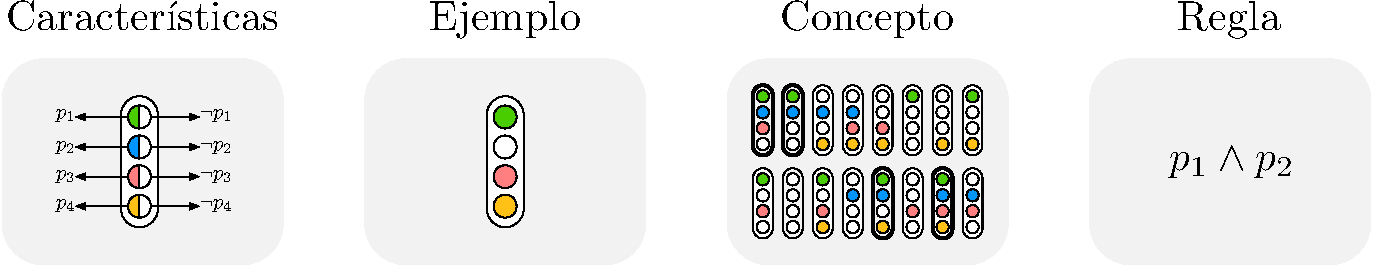
\includegraphics[scale=.6]{../figuras/pre/notacion.pdf}
\caption{Ilustración de las características $\{p_1,p_2,p_3,p_4\}$, el ejemplo $(1,0,1,1)$, y un concepto (los ejemplos positivos están marcados con bordes gruesos y los ejemplos negativos con bordes delgados). Se puede ver que la fórmula $p_3$ no es compatible con $\con$ pero $p_1 \oand p_2$, o $p_1 \oand p_2 \oand (p_3 \oor \lnot p_3)$, sí son compatibles con $\con$. $\overline \con$ puede describirse mediante $\lnot p_1\oor \lnot p_2$.}\label{semaforos}
\end{figure}

%In Figura~\ref{semaforos} we depict a concept $\con$ (variables are represented by colors) such that $\#\con=4$. One can see that the formula $x_3$ is not compatible with $\con$ but $x_1 \oand x_2$, or $x_1 \oand x_2 \oand (x_3 \oor \lnot x_3)$, are compatible with $\con$. $\overline \con$ may be described by $\lnot x_1\oor \lnot x_2$.

\paragraph{Complejidad para \gramboolxor.} Para el caso de la complejidad, definimos $|\varphi|$, el {\em tamaño} de la fórmula $\varphi\in\gramboolxor$, del mismo modo que en \grambool pero agregando un valor al operador adicional:
\begin{eqnarray*}
|\varphi\oxor\psi| &\eqdef& 1+|\varphi|+|\psi|.
\end{eqnarray*}


Si $\con$ es un conjunto de valuaciones sobre $\propvars$, definimos la {\em $\gramboolxor$-complejidad de la descripción mínima} de $\con$, notada $\mdlboolxor(\con)$, como el tamaño de la fórmula más corta cuya semántica es $\con$, es decir,
$$
\mdlboolxor(\con)\eqdef\min\{|\varphi|\mid \varphi\in L_{\gramboolxor},\sem{\varphi}=\con\}.
$$

Como $\grambool$ es un sublenguaje de $\gramboolxor$, tenemos que $\mdl{\gramboolxor}(\con)\leq\mdl{\grambool}(\con)$ para cualquier concepto $\con$.

\paragraph*{Ejemplo.}El concepto 
\begin{align*}
\con=\{&(1,0,0,0),(1,0,1,0),(1,0,0,1),(1,0,0,1)\\
&(0,1,0,0),(0,1,1,0),(0,1,0,1),(0,1,0,1)\},
\end{align*}
%which expresses that $x_1$ is true or $x_2$ is true but not both can be described in \gramboolxor as $\varphi=x_{1} \oxor x_{2}$, of length 3. In fact, one can check that this is the shortest formula compatible with $\con$, and so $\mdl{\gramboolxor}(\con)=3$. If we now switch to \grambool, we can no longer describe $\con$ as $x_{1} \oxor x_{2}$, since $\oxor$ is not part of its signature. However, in \grambool, the concept $\con$ may be described by  formula $\psi=(x_{1} \oand \neg x_{2}) \oor (x_{2} \oand \neg x_{1})$, of size 7. Since this formula has minimal size, we have that $\mdl{\grambool}(\con)=7$.
que expresa que $p_1$ es verdadero o $p_2$ es verdadero, pero no ambos, puede describirse en \gramboolxor como $\varphi=p_{1} \oxor p_{2}$, de tamaño 3. De hecho, se puede comprobar que esta es la fórmula más corta que describe a $\con$ (en el sentido de que $\sem{\varphi}=\con$), por lo que $\mdl{\gramboolxor}(\con)=3$. Si ahora cambiamos a \grambool, ya no podemos describir a $\con$ como $p_{1} \oxor p_{2}$, dado que $\oxor$ no es parte del lenguaje. Sin embargo, en \grambool, el concepto $\con$ puede describirse mediante la fórmula $\psi=(p_{1} \oand \neg p_{2}) \oor (p_{2} \oand \neg p_{1})$, de tamaño 7. Dado que esta fórmula tiene tamaño mínimo para ese concepto en \grambool, tenemos que $\mdl{\grambool}(\con)=7$.


\section{Experimento}


%\renewcommand*{\arraystretch}{1.2}
%\begin{table*}[!ht]
%\vspace{-0.5cm}
%\centering
%
%\begin{tabular}{|c|l l | c | c |l l | c | c|}
%\hline
%                                   &
%\multicolumn{2}{c|}{\textbf{Grupo objetivo}}       &
%\textbf{$\mdl{\gramboolxor}(\con)$} &
%\textbf{$\mdl{\grambool}(\con)$} &
%\multicolumn{2}{c|}{\textbf{Grupo control}}  &
%\textbf{$\mdl{\gramboolxor}(\con)$} &
%\textbf{$\mdl{\grambool}(\con)$} 
% \\ \hline
%\multirow{4}{*}{\parbox[t]{14mm}{\rotatebox[origin=c]{90}{\bf Entrenamiento}}} & \targeta & $x_{i}$             & 1 & 1                                                                  & \multicolumn{4}{c|}{$\longleftarrow$Ídem}                                                            \\ \cline{2-9}
%                                   &\targetb& $x_{i} \oxor x_{j}$       & 3 & 7 &\controlb& $x_{i} \oor x_{j}$  & 3 & 3                                                                  \\ \cline{2-9}
%                                  &\targetc & $x_{i} \oxor x_{j} \oxor x_{k}$ & 5 & 19 &\controlc& $x_{i} \oor (x_{j} \oand x_{k})$  & 5 & 5 \\ \cline{2-9}
%                                  &\targetd& $x_{k} \oxor x_{l}$       & 3 & 7&\controld&$x_{k} \oor x_{l}$  & 3 & 3                                                                  \\ \hline
%\multirow{2}{*}{\parbox[t]{2mm}{\rotatebox[origin=c]{90}{\bf Evaluación}}}  &\testa& $x_{i} \oand (x_{j} \oxor x_{k})$ & 5 & 9                 & \multicolumn{4}{c|}{$\longleftarrow$Ídem}                                                                                    \\ \cline{2-9}
%                               &\testb& $x_{i} \oand (x_{j} \oor x_{k})$  & 5 & 5         & \multicolumn{4}{c|}{$\longleftarrow$Ídem}                                                                                            \\ \hline
%\end{tabular}
%
%\caption{Secuencia de conceptos presentados en el %experimento: \targeta, \targetb, \targetc, \targetd, \testa, %\testb para el grupo objetivo y  \controla, \controlb, %\controlc, \controld, \testa, \testb para el grupo control. %Cada concepto $\con$ está representado por una fórmula %mínima $\varphi$ tal que $\sem{\varphi}=\con$. %Numbers $n/m$ on the right indicate $n=\mdl{\gramboolxor}(\con)$ and $m=\mdl{\grambool}(\con)$.
%MDL is measured as the number of operators and variables (excluding the \textit{not} operator) of the minimal formula with respect to the specified CFG.
%}
%\label{conceptos}
%\vspace{-0.4cm}
%\end{table*}



%55 participants participated in the experiment over the world wide web using the Amazon Mechanical Turk crowd sourcing platform. All were US residents over the age of 18 and had more than 95\% of past tasks successfully approved by other requesters. 44 participants completed the experiment through all the stages and declared not cheating (using pen, screenshots or a similar method to copy the answers) at the end of the experiment. Only data from these participants were used in the analyses reported below.\footnote{The learning times of all participants can be found in https://figshare.com/s/04d338adbbc4b1e83bf0.}

Un total de 55 personas participaron en el experimento a través de internet utilizando la plataforma de \textit{crowdsourcing} Amazon Mechanical Turk. Todos los participantes fueron residentes de EE.UU., mayores de 18 años y tenían más del 95\% de tareas pasadas aprobadas con éxito en la plataforma. Sólo 44 de ellos completaron todas las etapas del experimento y declararon no hacer trampas al final del experimento (se les aclaró que --aunque admitieran haber realizado anotaciones, capturas de pantalla o utilizado algún método similar-- igual serían calificados de manera positiva y recibirían su pago por haber realizado todas las etapas, pero que la información era crucial para los fines del análisis de los datos del experimento). En los análisis que se informan a continuación, sólo se utilizaron los datos de estos 44 participantes. \footnote{Los tiempos de aprendizaje de todos los participantes se pueden descargar en https://figshare.com/s/04d338adbbc4b1e83bf0.}

%Participants were divided randomly into a control group ($N=21$) and a target group ($N=23$). Both groups were presented with different sequences of six concepts. For each concept, there was a learning phase, a testing phase and a feedback phase. The average time spent in each concept was 167$\pm$20 s.e.m.\ seconds, and the average duration of the task was 21$\pm$4 s.e.m.\ minutes. After moving through the learning, testing and feedback phase of each of the six concepts, participants were asked if they used a pen or recorded the screen information in any way. They were also told that the answer to this question will not affect their payment, but that it was crucial for the experimenters to know.

Los participantes se dividieron aleatoriamente en un grupo de control ($N=21$) y en un grupo objetivo ($N=23$). A ambos grupos se les presentaron diferentes secuencias de seis conceptos. Para cada concepto, hubo una fase de {\em aprendizaje} y una fase de {\em entrenamiento-feedback}. La media del tiempo empleado en cada concepto fue de 167$\pm$20 s.e.m.\ segundos, y la duración promedio de la tarea fue de 21$\pm$4 s.e.m.\ minutos. 

%During the learning phase, all 16 items were presented in the screen (in random order), and items belonging to the concept were identified with bold boundaries, as shown in  Figura~\ref{semaforos}. Participants were told that only the items with bold boundaries were `blickets' (or `tufas', etc.: we used different words for each concept in the sequence), and asked them to try to identify what a blicket was. During the testing phase, the 16 items were shuffled in the screen, and participants were asked to click on items that were blickets. If they made mistakes after submitting their answer, they were directed to the feedback phase, in which items that were incorrectly classified were indicated with a red cross. After having studied the feedback, participants were redirected to the testing screen, where items were reshuffled. When every item was correctly classified, participants were asked to give a verbal description of the concept and then continued on to the following concept after a resting period. We characterize the subjective difficulty of each concept as the time the participant spent in learning, testing and feedback phases for that concept (excluding the time spent in the verbal description).



\begin{center}
\begin{table}[h]\small
\begin{tabular}{|c|c||c|c|c||c|c|c|}
\hline
\textbf{}                 & \textbf{Prueba} & \textbf{\begin{tabular}[c]{@{}c@{}}Grupo\\ Objetivo\end{tabular}} & \textbf{$\mdl{\gramboolxor}$} & \textbf{$\mdl{\grambool}$} & \textbf{\begin{tabular}[c]{@{}c@{}}Grupo\\ Control\end{tabular}} & \textbf{$\mdl{\gramboolxor}$} & \textbf{$\mdl{\grambool}$} \\ \hline
\multirow{4}{*}{\parbox[t]{2mm}{\rotatebox[origin=c]{90}{Entrenamiento\ \  \ \\ \ \  }}} & 1               & \begin{tabular}[c]{@{}c@{}}\targeta \\ $p_{i}$\end{tabular}                     & 1              & 1               & \multicolumn{3}{c|}{$\longleftarrow$ ídem}                                                                           \\ \cline{2-8} 
                          & 2               & \begin{tabular}[c]{@{}c@{}}\targetb\\ $p_{i} \oxor p_{j}$\end{tabular}                     & 3              & 7               & \begin{tabular}[c]{@{}c@{}}\controlb\\ $p_{i} \oor p_{j}$\end{tabular}                    & 3              & 3               \\ \cline{2-8} 
                          & 3               & \begin{tabular}[c]{@{}c@{}}\targetc \\ $p_{i} \oxor p_{j} \oxor p_{k}$\end{tabular}                     & 5              & 19              & \begin{tabular}[c]{@{}c@{}}\controlc\\ $p_{i} \oor (p_{j} \oand p_{k})$\end{tabular}                    & 5              & 5               \\ \cline{2-8} 
                          & 4               & \begin{tabular}[c]{@{}c@{}}\targetd\\ $p_{k} \oxor p_{l}$\end{tabular}                     & 3              & 7               & \begin{tabular}[c]{@{}c@{}}\controld\\$p_{k} \oor p_{l}$\end{tabular}                    & 3              & 3               \\ \hline
\multirow{2}{*}{\parbox[t]{2mm}{\rotatebox[origin=c]{90}{Eval.\ }}}     & 5               & \begin{tabular}[c]{@{}c@{}}\testa\\ $p_{i} \oand (p_{j} \oxor p_{k})$\end{tabular}                     & 5              & 9               & \multicolumn{3}{c|}{$\longleftarrow$ ídem}                                                                           \\ \cline{2-8} 
                          & 6               & \begin{tabular}[c]{@{}c@{}}\testb\\ $p_{i} \oand (p_{j} \oor p_{k})$\end{tabular}                     & 5              & 5               & \multicolumn{3}{c|}{$\longleftarrow$ ídem}                                                                           \\ \hline
\end{tabular}
\caption{Secuencia de conceptos presentados en el experimento: \targeta, \targetb, \targetc, \targetd, \testa, \testb para el grupo objetivo y  \controla, \controlb, \controlc, \controld, \testa, \testb para el grupo control. Cada concepto $\con$ está representado por una fórmula mínima $\varphi$ tal que $\sem{\varphi}=\con$}
\label{conceptos}
\end{table}
\end{center}

Durante la fase de {\em aprendizaje}, los 16 ejemplos (correspondientes a las 16 valuaciones posibles sobre $\propvars$ se presentaban en la pantalla (en orden aleatorio), y los elementos pertenecientes al concepto se identificaban con los bordes resaltados, como se muestra en la Figura~\ref{semaforos}. A los participantes se les decía que sólo los ejemplos resaltados eran `blickets' (o `tufas', etc.: usamos diferentes palabras para cada concepto en la secuencia), y se les pedía que intentaran identificar qué era un `blicket'. Durante la etapa de {\em entrenamiento}, los 16 ejemplos eran mezclados y mostrados en la pantalla, y se les pedía que hicieran clic en aquellos ejemplos que eran blickets. Si al enviar su respuesta cometían errores, se los dirigía a la pantalla de {\em feedback} donde los ejemplos que se clasificaron incorrectamente se marcaban con una cruz roja. Luego de haber estudiado la respuesta, los participantes eran redirigidos a la pantalla de prueba, donde los ejemplos eran nuevamente mezclados y mostrados en pantalla para su selección. Esto se repetía hasta que los participantes seleccionaran correctamente todos los ejemplos. Una vez que la selección era correcta, se les pedía que dieran una descripción verbal del concepto y luego continuaban con el siguiente concepto tras un breve período de descanso. Caracterizamos la dificultad subjetiva de cada concepto como el tiempo que un participante pasó en las fases de {\em aprendizaje} y e {\em entrenamiento-feedback} para cada concepto (excluyendo el tiempo dedicado a la descripción verbal). Una visión esquemática del experimento se puede ver en la Figura~\ref{fig:experimentoPRE}.

\begin{figure}
\begin{center}
  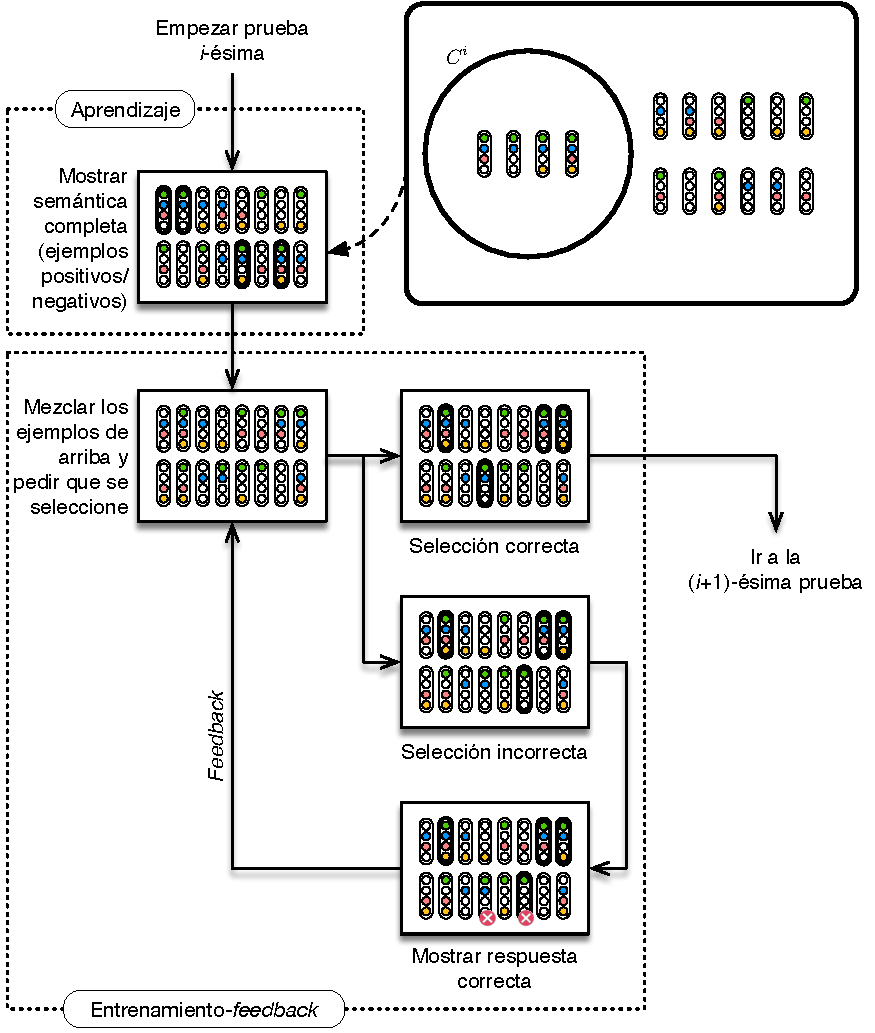
\includegraphics[scale=1]{../figuras/pre/experimento_PRE.pdf}
\end{center}\caption{El esquema de funcionamiento del experimento.}\label{fig:experimentoPRE}
\end{figure}


%Both groups (target and control), were exposed to 6 concepts. The second, third and fourth concepts are {\em training} concepts, and were different between both groups. The last two concepts are the {\em test} concepts, and were the same for both groups. The first concept was the trivial concept $x_i$ for both groups, which was aimed to get participants started in the task. Importantly, variables (i.e. color lights inside objects in Figura~\ref{semaforos}) were randomized for every concept, so paying selective attention to a specific variable across subsequent concepts was not beneficial for learning the concept sequence.

Ambos grupos (objetivo y control), fueron expuestos a 6 conceptos. El segundo, tercero y cuarto concepto son los conceptos de {\em entrenamiento} y fueron diferentes para cada grupo. Los últimos dos conceptos son los conceptos de {\em evaluación}, y fueron los mismos para ambos grupos. El primer concepto fue el concepto trivial $x_i$ para ambos grupos, cuyo objetivo fue que los participantes se familiarizaran con la tarea. Es importante destacar que las variables (es decir, las luces de color dentro de los ejemplos en la Figura~\ref{semaforos}) fueran seleccionadas de manera aleatoria para cada concepto, por lo que prestar atención selectiva a una característica específica a lo largo de la secuencia de conceptos (por ejemplo, la luz roja) no era beneficioso para aprender.

%As shown in Table~\ref{conceptos}, we presented the target group with training concepts which are succinctly described when $\oxor$ is part of the language, but necessarily described with lengthier formulas if $\oxor$ is absent; more technically, concepts for which $\mdl{\gramboolxor}$ is much smaller than $\mdl{\grambool}$. We also corroborated that for \targetb, \targetc, \targetd and \testa the number of formulas in $\gramboolxor$ with length strictly smaller than $\mdl{\grambool}$ was at least 10 times greater than the number of formulas in $\grambool$ with length equal to $\mdl{\grambool}$.

Como se muestra en la Tabla~\ref{conceptos}, presentamos al grupo objetivo conceptos de entrenamiento que se describen sucintamente cuando $\oxor$ es parte del lenguaje, pero que necesariamente se describen con fórmulas más largas si $\oxor$ está ausente; más técnicamente, conceptos para los que $\mdl{\gramboolxor}$ es mucho más pequeño que $\mdl{\grambool}$. También corroboramos que para \targetb, \targetc, \targetd y \testa, el número de fórmulas en $\gramboolxor$ con una longitud estrictamente menor que $\mdl{\grambool}$ era al menos 10 veces mayor que el número de fórmulas en $\grambool$ con longitud igual a $\mdl{\grambool}$.

%Participants in the control group, on the other hand, experienced a sequence of concepts that could be easily described using the language given by \grambool. After these training concepts, both groups were presented with the same pair of test concepts: one which could be only succinctly described in \gramboolxor, and one for which the MDL did not depend on the underlying language \gramboolxor or \grambool. We compared learning times between the two groups for these last two concepts.

Los participantes en el grupo control, por otro lado, experimentaron una secuencia de conceptos que podía describirse fácilmente usando el lenguaje dado por \grambool. Después de estos conceptos de entrenamiento, a ambos grupos se les presentó el mismo par de conceptos de evaluación: uno que sólo podía ser descrito sucintamente en \gramboolxor (es decir, $\mdlboolxor<\mdlbool$), y uno para el que el la complejidad de descripción no dependía si el lenguaje subyacente era \gramboolxor o \grambool (es decir, $\mdlboolxor=\mdlbool$). Comparamos los tiempos de aprendizaje entre los dos grupos para estos dos últimos conceptos.


%As shown in Table~\ref{conceptos}, training concepts for the target (xor) group were: $x_{i}$, $x_{i} \oxor x_{j}$, $x_{i} \oxor x_{j} \oxor x_{k}$, and $x_{k} \oxor x_{l}$, called \targeta, \targetb, \targetc and \targetd respectively. Training concepts for the control group were: $x_{i}$, $x_{i} \oor x_{j}$, $x_{i} \oor (x_{j} \oand x_{k})$, and $x_{k} \oor x_{l}$ called \controla, \controlb, \controlc and \controld respectively. We use the indexes \textit{i, j, k, l} instead of numbers because variables were randomized in each trial. $x_{i}$ could stand for $x_1$, $x_2$, $x_3$ or $x_4$, that is, for any of the four colors. After these four concepts, both groups were presented with the same test concepts: $x_{i} \oand (x_{j} \oxor x_{k})$, and $x_{i} \oand (x_{j} \oor x_{k})$, called \testa and \testb respectively.

Como se muestra en la Tabla~\ref{conceptos}, los conceptos de entrenamiento para el grupo objetivo (xor) fueron: $p_{i}$, $p_{i} \oxor p_{j}$, $p_{i} \oxor p_{j} \oxor p_{k}$, y $p_{k} \oxor p_{l}$, llamados \targeta, \targetb, \targetc y \targetd respectivamente. Los conceptos de entrenamiento para el grupo control fueron: $p_{i}$, $p_{i} \oor p_{j}$, $p_{i} \oor (p_{j} \oand p_{k})$, y $p_{k} \oor p_{l}$ llamados \controla, \controlb, \controlc y \controld respectivamente. Usamos los índices \textit{i, j, k, l} en lugar de números porque las variables fueron elegidas de manera aleatoria en cada ensayo. Así, $p_{i}$ podría representar $p_1$, $p_2$, $p_3$ o $p_4$, es decir, cualquiera de los cuatro colores. Después de estos cuatro conceptos, a ambos grupos se les presentaron los mismos conceptos de evaluación: $p_{i} \oand (p_{j} \oxor p_{k})$, y $p_{i} \oand (p_{j} \oor p_{k})$, llamados \testa y \testb respectivamente.

%Choosing which concepts to show the target group in order for them to `learn' the $\oxor$ operator is critical in our experiment. Crucially, the learner must have an option between two alternatives that describe the concept: one that is succinct but uses $\oxor$, or necessarily a much longer one in the absence of $\oxor$. In other words, these concepts must be compatible with short logical formulas if and only if we take \gramboolxor as the language of description. To ensure that this was the case, we enumerated, for each concept, all formulas compatible with it and produced by the \grambool and \gramboolxor grammars up to length 19. For all training concepts of the target group, the shortest compatible formula without $\oxor$ is much longer than the shortest compatible formula with $\oxor$. This is shown in Table\ref{conceptos}.

Elegir qué conceptos mostrar al grupo objetivo para que `aprendan' el operador $\oxor$ es una parte clave de nuestro experimento. El sujeto debe tener una opción entre dos alternativas que describan el concepto: una que es sucinta pero usa el operador $\oxor$, o una que sea necesariamente mucho más larga en ausencia del $\oxor$. En otras palabras, estos conceptos deben ser compatibles con fórmulas lógicas cortas si y sólo si tomamos \gramboolxor como el lenguaje de descripción. Para asegurarnos de que este fuera el caso, enumeramos, para cada concepto, todas las fórmulas compatibles con él que se puedan producir con las gramáticas \grambool y \gramboolxor hasta la longitud 19. Para todos los conceptos de entrenamiento del grupo objetivo, la fórmula compatible más corta sin $\oxor$ es mucho más larga que la fórmula compatible más corta con $\oxor$ (es decir $\mdlboolxor\ll\mdlbool$). Esto se muestra en la Tabla~\ref{conceptos}.

%\section{Model-Free Results}
\section{Resultados sin modelo}

%We measure the subjective difficulty of a given concept as the total time needed by the participant to successfully encode the concept, which indicates that they can reliably express which exemplars belong to the concept and which do not.

Medimos la dificultad subjetiva de un concepto dado como el tiempo total que necesita el participante para codificar con éxito el concepto, lo que indica que pueden expresar qué ejemplos perteneces al concepto y cuáles no.


%Participants from the target group spent almost half the time than participants from the control group in \testa, which could be succinctly described only in \gramboolxor ($111\pm16$ s.e.m.\ seconds versus $214\pm37$ s.e.m.\ seconds, a two-sample t-test reveals $t_{42}=2.6$, $P<0.01$), as shown in Figura~\ref{model free} (a). We also found that the control group learned much faster \testb ($143\pm14$ s.e.m.\ seconds for the target group versus $76\pm10$ s.e.m.\ seconds for the control group, $t_{42}=3.5$, $P<0.01$). A mixed ANOVA with \testa-\testb as within subject factor and target-control groups as between subject factor reveals a strong interaction between group and \testa-\testb ($F=15.3$, $P<0.001$), indicating that the differences in learning times for \testa and \testb were very different between the two groups.

Los participantes del grupo objetivo pasaron casi la mitad del tiempo que los participantes del grupo control en \testa, que podía describirse sucintamente sólo en \gramboolxor ($111\pm16$ s.e.m.\ segundos contra $214\pm37$ s.e.m.\ segundos, un t-test para dos muestras revela $t_{42}=2.6$, $p<0.01$), como se muestra en la Figura.~\ref{model free} (a). También encontramos que el grupo de control aprendió mucho más rápido \testb ($143\pm14$ s.e.m.\ segundos para el grupo objetivo contra $76\pm10$ s.e.m.\ segundos para el grupo control, $t_{42}=3.5$, $p<0.01$). Un ANOVA mixto con \testa-\testb como factor dentro de los sujetos y grupos objetivo-control como factor entre sujetos revela una fuerte interacción entre el grupo y \testa-\testb ($F=15.3$, $P<0.001$), lo que indica que las diferencias en el aprendizaje de los tiempos para \testa y \testb fueron muy diferentes entre los dos grupos.

%The target group encoded \testa more efficiently than the control group. We propose that the control group expected to find in \testa and \testb structures that could be easily built in \grambool. The target group, on the other hand, became biased towards the $\oxor$ structure, and they expected to find it in \testa and \testb. This caused \testa to be encoded more rapidly by the target group and \testb more rapidly by the control group. Assuming that the subjective difficulty of learning a concept is proportional to the complexity of its internal representation, we conclude that after exposure to the training concepts, participants in the target group represented the $\oxor$ more efficiently than the control group, and expected to find this structure in \testa and \testb.

El grupo objetivo codificó \testa de manera más eficiente que el grupo control. Proponemos que el grupo control esperaba encontrar en \testa y \testb estructuras que pudieran ser fácilmente descriptas en \grambool. El grupo objetivo, por otro lado, se inclinó hacia la estructura $\oxor$, y esperaban encontrarlo en \testa y \testb. Esto provocó que \testa se codificara más rápido por el grupo objetivo y \testb más rápido por el grupo control. Suponiendo que la dificultad subjetiva de aprender un concepto es proporcional a la complejidad de su representación, llegamos a la conclusión que --después de la exposición a los conceptos de entrenamiento-- los participantes en el grupo objetivo representaron el $\oxor$ de manera más eficiente que el grupo control, y esperaban encontrar esta estructura en \testa y \testb.



\begin{figure}[t!]
      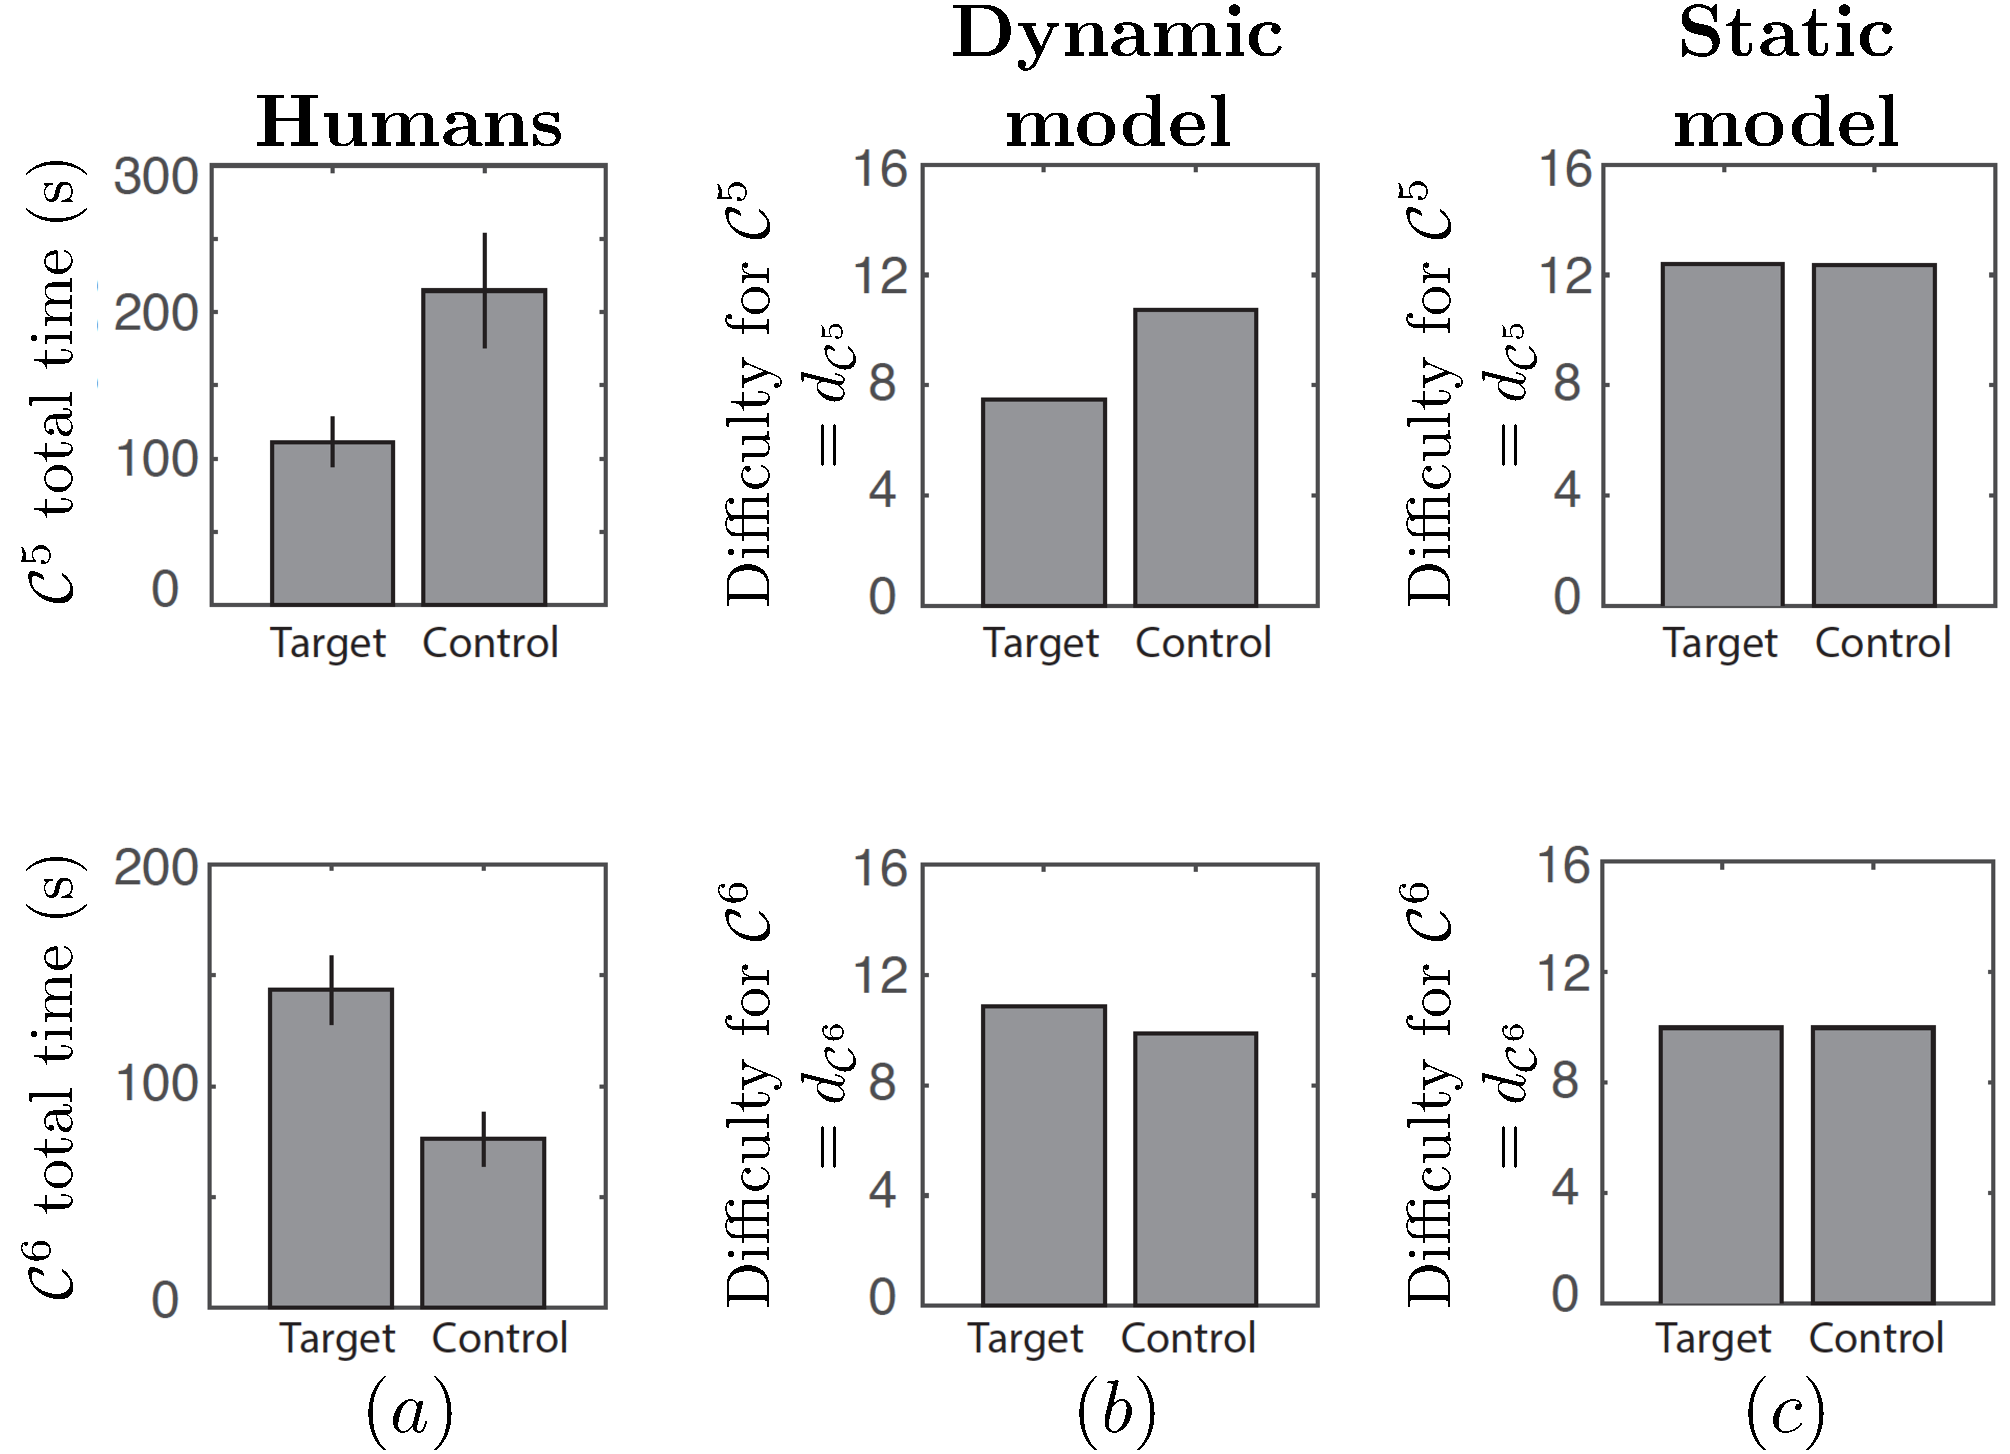
\includegraphics[scale=0.4]{model_free-3.pdf}
      \centering
      %\caption{Concept learning time $(a)$ and difficulty predicted $(b)$, $(c)$ for the two test concepts (\testa and \testb). Error bars are s.e.m.\ across subjects.}
      \caption{Tiempo de aprendizaje del concepto $(a)$ y dificultad pronosticada $(b)$, $(c)$ para los dos conceptos de evaluación (\testa y \testb). Las barras de error son s.e.m.\ entre los sujetos}
      \label{model free}
   \end{figure}
\section{Modelo}

%When presented with a concept (e.g.~Figura~\ref{semaforos}), our model generates logical formulas and evaluate them to true or false for that concept, keeping the formula only if it is true. To generate formulas, the model uses a symbolic language in which each rule (symbols and operators) is associated with a probability of being used. The probability of generating a formula is proportional to the product of the probabilities of the rules required for building it, and therefore it decreases exponentially with its length. Furthermore, if one of the rules has a very low probability of being used, formulas that require it will also have very low probability.


Cuando se le presenta un concepto, nuestro modelo genera fórmulas lógicas y las evalúa como verdaderas o falsas para ese concepto, manteniendo la fórmula sólo si es verdadera. Para generar fórmulas, el modelo utiliza un lenguaje simbólico en el que cada regla de producción (símbolos y operadores) está asociado con una probabilidad de ser utilizada. La probabilidad de generar una fórmula es proporcional al producto de las probabilidades de las reglas requeridas para construirla y, por lo tanto, disminuye exponencialmente con su longitud. Además, si una de las reglas tiene una probabilidad muy baja de ser utilizada, las fórmulas que la requieran también tendrán una probabilidad muy baja.


%The \textit{Static model} maintains the rules' probabilities fixed throughout the concept sequence (the 6 concepts in Table~\ref{conceptos}). The \textit{Dynamic model} updates the probabilities after each concept, in order to minimize the expected description length of future concepts, assuming they have similar structure to the concepts learnt so far. We include in this model the $\oxor$ rule a priori in the language, but with vanishing probability of being used. Changes in this probability can be analogously interpreted as the probability that a rational agent without the compiled symbol a priori decides to add the compiled expression as a new primitive into her language. %This means that our model will fit somewhere between the computational and the algorithmic level of analysis by Marr's~\cite{marr1979computational,griffiths2015rational}. It can explain algorithmically how learning occurs, however, adding a new primitive is not modeled entirely at this level. The vanishing probability analogy is sufficient to make the new primitive be highly unlikely to be used without exposure and to allow it to emerge after concepts. Still, it does not explain --at an algorithmic level-- how any new primitive can arise, leaving the mechanics of the language change between the computational and algorithmic level.

El \textit{modelo estático} mantiene las probabilidades de las reglas fijas a lo largo de la secuencia de conceptos (los 6 conceptos de la Tabla~\ref{conceptos}). El \textit{modelo dinámico} actualiza las probabilidades después de cada concepto, con el fin de minimizar la longitud de descripción esperada de conceptos futuros, asumiendo que tienen una estructura similar a los conceptos aprendidos hasta ahora. Incluimos en este modelo el operador $\oxor$ a priori en el lenguaje, pero con una probabilidad de ser utilizado muy baja. Cambios en esta probabilidad se pueden interpretar análogamente como la probabilidad de que un agente racional sin el símbolo compilado a priori decida agregar la expresión compilada como un nuevo operador en su lenguaje.


\subsection{Modelo estático}

\newcommand{\form}{\varphi}
%Under the \lot assumption,  given a concept $\con$ (e.g.\ Figura~\ref{semaforos}), the probability that an agent uses formula $\form$ to explain this concept is defined by Bayes theorem: 
Bajo la hipótesis de \lot,  dado un concepto $\con$, la probabilidad de que un agente use la fórmula $\form$ para explicar el concepto está definida por el teorema de Bayes: 
$$
P(\form\mid \con) \propto P(\con\mid \form)P(\form).
\label{Bayes fix}
$$
% \begin{equation}
% P(\form\mid \con) \propto P(\con\mid \form)P(\form).
% \label{Bayes fix}
% \end{equation}
%
%The likelihood $P(\con\mid \form)$ of a logical statement $\form$ can be simply defined as 1 if $\sem{\form}=\con$ and 0 otherwise. In other words, for any given concept, only explanations that describe this concept are considered as possible explanations. The likelihood term has been defined more flexibly in the literature~\cite{goodman2008rational,piantadosi2016logical}, allowing for mislabeled elements. We keep this simpler definition in order to reduce the number of free parameters of the model, as we do not intend to account for mislabeling errors in our experiment.

La función de verosimilitud $P(\con\mid \form)$ de un enunciado lógico $\form$ se puede definir simplemente como 
$$
P(\con\mid \form)=
\begin{cases}
1 & \mbox{si $\sem{\form}=\con$;}\\
0 & \mbox{en caso contrario.}
\end{cases}
$$
% 1 si $\sem{\form}=\con$ y 0 en caso contrario. 
En otras palabras, para cualquier concepto dado, sólo las explicaciones que describen este concepto se consideran como posibles explicaciones. Se ha definido la función de verosimilitud de manera más flexible en la literatura~\cite{goodman2008rational,piantadosi2016logical}, permitiendo elementos mal etiquetados. Mantenemos esta definición más simple para reducir el número de parámetros libres del modelo ya que no pretendemos tener en cuenta los errores de etiquetado en nuestro experimento.

%The prior $P(\form)$ is defined by augmenting the context-free grammars shown in Figura~\ref{PCFG} into a probabilistic context-free grammars (PCFG). In the PCFG, each rule has associated a parameter indicating the probability of using that rule. A PCFG can be used to produce logical statements similar to a CFG. Each non-terminal remaining in the statement is expanded using a rule of the PCFG with probability proportional to that rule's associated parameter, until no non-terminals remain in the statement. 

Al igual que en el Capítulo~\ref{chapter:PO}, la probabilidad a priori $P(\form)$ se define aumentando las gramáticas libre de contexto (CFG) \grambool y \gramboolxor en gramáticas probabilísticas libres de contexto (PCFG). En la PCFG, cada regla tiene asociado un parámetro que indica la probabilidad de utilizar esa regla. Se puede utilizar una PCFG para producir enunciados lógicos de manera similar a una CFG. Cada no-terminal en la expresión es expandido usando una regla de la PCFG con probabilidad proporcional al parámetro asociado a la regla hasta que no queden no-terminales en la expresión.


%We assume that the probability that a subject uses formula $\form$ to explain concept $\con$ is proportional to the posterior $P(\form \mid \con)$, and the subjective difficulty $d_\con$ of a concept $\con$ to a participant is proportional to the length of the formula that the participant is using to explain that concept. However, there is no way to know directly which internal formula $\form$ the participant is using (and therefore we do not know $|\form|$). Hence, the most parsimonious approach is to consider the entire posterior distribution $\textbf{P}(\form \mid \con)$ over possible formulas.\footnote{This is equivalent to the Sampling Hypothesis described in~\cite{denison2013rational}, by which participants represent distributions through samples. Similar results are obtained if each participant carries entire probability distributions.}

Suponemos que la probabilidad de que un sujeto utilice la fórmula $\form$ para explicar el concepto $\con$ es proporcional a la probabilidad a posteriori $P(\form \mid \con)$, y que la dificultad subjetiva $d_\con$ de un concepto $\con$ para un participante es proporcional a la longitud de la fórmula que el participante está usando para explicar ese concepto. Sin embargo, no hay forma de saber directamente qué fórmula interna $\form$ está utilizando el participante (y, por tanto, no sabemos $|\form|$). Por lo tanto, el enfoque más parsimonioso consiste en considerar la distribución a posteriori $P(\form \mid \con)$ de manera completa sobre todas las posibles fórmulas.
%\footnote{Esto es equivalente a la hipótesis de muestreo descripta en~\cite{denison2013rational}, por la cual los participantes representan distribuciones a través de muestras. Se obtienen resultados similares si cada participante traslada la distribución de probabilidad completa} \sergio{no estoy seguro de cómo explicarlo}

%Given a concept $\con$, the expected length $E_\con$ of the formulas used by the participant is simply
Dado un concepto $\con$, la longitud esperada $E_\con$ de las fórmulas utilizadas por el participante es simplemente
%
 \begin{equation}
E_\con=\sum_{\sem{\form}=\con} |\form| \ P(\form \mid \con),
 \label{expected length}
 \end{equation}
%
%where the sum is over all formulas $\varphi$ compatible with $\con$. We  define the difficulty $d_\con$ of a concept experienced by the participant  as $$d_\con \propto E_\con + \alpha N_\con,$$
donde la suma es sobre todas las fórmulas $\varphi$ compatibles con $\con$. Definimos la dificultad $d_\con$ de un concepto experimentado por un participante como $$d_\con \propto E_\con + \alpha N_\con,$$
%
% \begin{equation}
%d_\con \propto E_\con + \alpha N_\con,
% \label{length}
% \end{equation}
%
%where we added a term that accounts for the cardinality of the concept: $N_\con$ is the cardinality of the concept or its complement, the one being smaller, i.e.\ $N_\con=\min \{ \#\con, \#\overline \con\}$ (e.g.\ $N_\con=4$ for the concept $\con$ of  Figura~\ref{semaforos}), and $\alpha$ is a free parameter fitted globally for all concepts and participants to its maximum likelihood value of 0.9. In this way, we remove the asymmetry between positive and negative examples, while accounting for the toil taken by considering a larger number of items simultaneously.
donde agregamos un término que da cuenta de la cardinalidad del concepto: $N_\con$ es la cardinalidad del concepto o su complemento, el que sea más pequeño, es decir, i.e.\ $N_\con=\min \{ \#\con, \#\overline \con\}$ (por ejemplo, \ $N_\con=4$ para el concepto $\con$ de la Figura~\ref{semaforos}), y $\alpha$ es un parámetro libre ajustado globalmente para todos los conceptos y participantes hasta su valor de máxima verosimilitud: $0.9$. De esta manera, eliminamos la asimetría entre ejemplos positivos y negativos, mientras se sigue contabilizando el esfuerzo que lleva considerar un número más grande de ejemplos de manera simultánea.

%In practice, to approximate $E_\con$ for each concept $\con$, we calculated the posterior probability $P(\form\mid \con)$ of all compatible formulas $\form$s up to size 19 with $P(\form\mid \con)$ and then use ~\eqref{expected length}. Since the space of all possible $\form$s grows exponentially with $|\form|$, normative procedures for estimating $P(\form\mid \con)$ in this space involve stochastic search algorithms. However, in our case, we were able to exhaustively enumerate and calculate the posterior probability of \textit{all} formulas generated by the PCFG up to a sufficiently high size $M$ such that all formulas with $|\form|>M$ have vanishing probabilities when compared to shorter compatible formulas for the current concept (because the prior $P(\form)$ decreases exponentially with the size of the formula).

En la práctica, para aproximar $E_\con$ para cada concepto $\con$, calculamos la probabilidad a posteriori $P(\form\mid \con)$ de todas las fórmulas compatibles $\form$ hasta longitud 19 con $P(\form\mid \con)$ y luego utilizamos~\eqref{expected length}. Dado que el espacio de todas las posibles $\form$ crece exponencialmente con $|\form|$, los procedimientos normativos para estimar $P(\form\mid \con)$ en este espacio implican algoritmos de búsqueda estocásticos. Sin embargo, en nuestro caso, pudimos enumerar y calcular exhaustivamente la probabilidad a posteriori de todas las fórmulas generadas por la PCFG hasta un nivel suficientemente alto de longitud $M$ tal que todas las fórmulas con $|\form|>M$ tienen probabilidades insignificantes en comparación con las fórmulas compatibles más cortas para el concepto actual (porque la probabilidad a priori $P(\form)$ decrece exponencialmente con la longitud de la fórmula).

\subsection{Modelo dinámico}

%Up to this point, we assumed that, given a concept $\con$, the posterior distribution over formulas $P(\form\mid \con)$ was independent of the other concepts presented in the sequence. However, if the \lot (i.e. the PCFG) updates with experience, the prior $P(\form)$ in $P(\form\mid \con)$ will change, and so will $E_\con$ in \eqref{expected length} and finally the subjective difficulty $d_\con$. Therefore, $d_\con$ will depend on the sequence of concepts that were previously presented to the participant.

Hasta este punto asumimos que, dado un concepto $\con$, la distribución a posteriori sobre las fórmulas $P(\form\mid \con)$ era independiente de los conceptos presentados en la secuencia. Sin embargo, si el \lot (es decir, la PCFG) se actualiza con la experiencia, la probabilidad a priori $P(\form)$ en $P(\form\mid \con)$ cambiará, al igual que $E_\con$ en \eqref{expected length} y finalmente también la dificultad subjetiva $d_\con$. Por lo tanto, $d_\con$ dependerá de la secuencia de conceptos que se presentaron previamente al participante.

En otras palabras, dado que ahora $P(\form)$ depende de la secuencia de conceptos observada por el participante, en lugar de $P(\form\mid \con)$, tendremos 
$$
P(\form\mid \con^{t},\dots,\con^{1}) \propto P(\con^{t}\mid \form)P(\form\mid \con^{1},\dots,\con^{t-1}),
$$ 
% \begin{equation}
% P(\form\mid \con^{t}) \propto P(\con^{t}\mid \form)P(\form\mid \con^{1},\dots,\con^{t-1}),
% \label{Bayes}
% \end{equation}
%
%where $\con^{t}$ is the concept presented at trial~$t$, and $P(\form\mid \con^{1},\dots,\con^{t-1})$ depends on the state of the PCFG at trial $t$, which in turn depends on how the PCFG gets updated from trial to trial.
donde $\con^{t}$ es el concepto presentado en la tarea~$t$, y $P(\form\mid \con^{1},\dots,\con^{t-1})$ depende del estado de la PCFG en la tarea $t$, que a su vez depende de cómo se actualiza la PCFG entre cada tarea.

%Intuitively, the update process increases the probability of using a certain rule in the PCFG accordingly to how useful this rule was to compress compatible formulas for the concepts previously learned in the same domain. Specifically, we model the update process in a normative manner: the probability of using a rule of the PCFG at trial $t$ is equal to the Bayesian posterior probability that this rule will enable the learner to find compressed explanations at trial $t$, according to how useful it was to compress explanations in trials $1,\dots,t-1$.

Intuitivamente, el proceso de actualización aumenta la probabilidad de utilizar una determinada regla en la PCFG de acuerdo con la utilidad de esa regla para comprimir fórmulas compatibles para conceptos aprendidos previamente en el mismo dominio. Específicamente, modelamos el proceso de actualización de manera normativa: la probabilidad de utilizar una regla de la PCFG en la tarea $t$ es igual a la probabilidad a posteriori de que esta regla permita al sujeto encontrar explicaciones comprimidas en la tarea $t$, de acuerdo con la utilidad de comprimir explicaciones en las tareas $1,\dots,t-1$.

%To formalize the update of the PCFG, we define $P(\form)$ similarly to~\cite{goodman2008rational}. Specifically, the prior probability of a logical statement at trial $t$ in the concept sequence uses a single Dirichlet-multinomial for the set of rule expansions. The Dirichlet is parameterized by a set of positive real numbers $D_{i}^{t}$, one for each rule $i$ in the PCFG, which in turn determine the probability of using rule $i$ at trial $t$: a higher $D_{i}$ indicates a higher probability of using rule $i$.

Para formalizar la actualización de la PCFG, definimos $P(\form)$ de manera similar a~\cite{goodman2008rational}. Específicamente, la probabilidad a priori de una expresión lógica en la tarea $t$ en la secuencia de conceptos usa una Dirichlet  multinomial para el conjunto de reglas. La distribución Dirichlet  está parametrizada por un conjunto de números reales positivos $D_{i}^{t}$, uno por cada regla $i$ en la gramática, que a su vez determinan la probabilidad de utilizar la regla $i$ en la tarea $t$: una $D_{i}$ más alta indica una mayor probabilidad de utilizar la regla $i$.

%The prior is specified by the set Dirichlet parameters $\textbf{D}^{0}$ with which we start the experiment ($\textbf{D}^{0}$ represents a vector containing the prior parameters of all rules in the grammar at trial 0). In our experiment, we set the prior Dirichlet parameters of all rules equal to 1, and the parameter of the rule that expands the target operator to a value several orders of magnitude smaller ($\approx 10^{-4}$). This means that the target operator was practically absent at the beginning of the experiment, but it was technically possible to `learn it' by increasing its probability as the experiment developed.

La probabilidad a priori está especificada como el conjunto de parámetros de la Dirichlet $\textbf{D}^{1}$ con el que iniciamos el experimento ($\textbf{D}^{1}$ representa un vector que contiene los parámetros a priori de todas las reglas para la tarea 1). En nuestro experimento, establecemos los parámetros a priori de todas las reglas en 1, excepto por el de la regla que expande el operador objetivo $\oxor$ que está establecido con un valor varios órdenes de magnitud menor ($\approx 10^{-4}$). Esto significa que el operador objetivo está prácticamente ausente al comienzo del experimento, pero que es técnicamente posible `aprenderlo' si se aumenta su probabilidad a medida que se desarrolla el experimento.

%Under the Dirichlet model, the prior $P(\form\mid \con^{1},\dots,\con^{t-1})$ can be rewritten using the Dirichlet parameters as $P(\form\mid\textbf{D}^{t})$. Therefore, to know how $P(\form\mid \con)$ updates from trial to trial, we only need to know how $\textbf{D}$ updates from trial to trial.

Bajo el modelo de Dirichlet, la probabilidad a priori $P(\form\mid \con^{1},\dots,\con^{t-1})$ se puede reescribir utilizando los parámetros de la Dirichlet como $P(\form\mid\textbf{D}^{t})$. Por lo tanto, para saber cómo se actualiza $P(\form\mid \con)$ entre cada tarea, sólo necesitamos saber cómo se actualiza  $\textbf{D}$ entre cada tarea.

%The Dirichlet parameter of rule $i$ at trial $t+1$ is equal to its parameter at trial $t$ plus the amount of times the production $i$ was used in generating all formulas compatible with the concept at trial $t$ (we note $M_{i}(\form)$ as the number of times that rule $i$ is used in generating formula $\form$), weighted by each formula's posterior probability at trial $t$:

El parámetro Dirichlet de la regla $i$ en la tarea $t+1$ es igual al parámetro en la tarea $t$ más la cantidad de veces que se utilizó la regla $i$ para generar todas las fórmulas compatibles con el concepto en la tarea $t$ (definimos a $M_{i}(\form)$ como el número de veces que la regla $i$ es usada para generar la fórmula $\form$), ponderada por la probabilidad a posteriori de cada fórmula en la tarea $t$:
 \begin{equation}
 D_{i}^{t+1}=D_{i}^{t}+\sum_{\sem{\form}=\con^t} P(\form\mid \textbf{D}^{t}) \ M_{i}(\form). 
 \label{Dirichlet}
 \end{equation}
 %
%This Bayesian learning mechanism increases the probability of using rules that allow concepts to be succinctly described. This happens because these formulas have higher probability $P(\form\mid \textbf{D})$ than longer formulas, so the Dirichlet parameters of the rules that build these formulas increase more strongly than those of the rules that build longer formulas.   
%
Este mecanismo de aprendizaje bayesiano aumenta la probabilidad de utilizar reglas que permitan describir conceptos de manera sucinta. Esto sucede porque estas fórmulas tienen mayor probabilidad $P(\form\mid \textbf{D})$ que fórmulas más largas, por lo que los parámetros Dirichlet de las reglas que construyen estas fórmulas aumentan con más fuerza que los de las reglas que construyen fórmulas más largas.   

% \section{Results}
\section{Resultados}

% The Bayesian agent that minimizes the expected complexity of future concepts by optimally adapting its \lot to the inferred structure of the task accurately captures the dynamics of human learning across concepts. If we did not allow the model to update the probability of the operators after each concept, and particularly the compiled operator $\oxor$, the control group and the target group would be indistinguishable to the model as it would predict equal average formula length for both groups (see Figura~\ref{model free}, {\em Static Model}). Instead, as shown in Figura~\ref{results}, by adjusting the prior probabilities based on concept exposure the dynamic model is able to capture learning time patterns in the target groups ($R^{2}=0.96$ compared to $R^{2}=0.73$ for the static model). Expectedly, both models perform similarly in the control groups as they were designed to not encourage the use of any particular operator ($R^{2}=0.72$; $R^{2}=0.71$ for the static model). The impact of the learning capability of the model is most evident in the target group concept sequence, which was designed to this effect. If the structure of the concepts does not bias the \lot primitives one way or the other, it is expected that a static model will provide a reasonable fit. However, it is difficult to tell a priori how unbiased a set of concepts really is, so experiments relying on repeated concept exposure should always take between-concept learning into account. 
El agente bayesiano que minimiza la complejidad esperada de los conceptos futuros adaptando de manera óptima su \lot a la estructura inferida de la tarea captura con precisión la dinámica del aprendizaje humano a través de los conceptos. Si no permitiéramos que el modelo actualizara la probabilidad de los operadores después de cada concepto --y particularmente del operador compilado $ \oxor $--, el grupo control y el grupo objetivo serían indistinguibles desde el modelo, ya que prediría la misma longitud promedio de fórmula en ambos grupos (ver Figura~\ref{model free}, {\em Modelo estático}). En cambio, como se muestra en la Figura~\ref{results}, al ajustar las probabilidades a priori basadas en la exposición del concepto, el modelo dinámico es capaz de capturar patrones de tiempo de aprendizaje en los grupos objetivo ($ R^{2} = 0.96 $ en comparación con $ R^{2} = 0.73 $ para el modelo estático). Como era de esperar, ambos modelos funcionan de manera similar en los grupos de control, ya que fueron diseñados para no fomentar el uso de ningún operador en particular ($ R^{2} = 0.72 $; $ R^{2} = 0.71 $ para el modelo estático). El impacto de la capacidad de aprendizaje del modelo es más evidente en la secuencia de conceptos del grupo objetivo, que se diseñó a tal efecto. Si la estructura de los conceptos no sesga las primitivas de \lot de una forma u otra, se espera que un modelo estático proporcione un ajuste razonable. Sin embargo, es difícil decir a priori qué tan imparcial es realmente un conjunto de conceptos, por lo que los experimentos que se basan en la exposición repetida de conceptos siempre deben tener en cuenta el aprendizaje entre conceptos.

% Allowing the model to constantly update its beliefs from concept to concept is a requisite to capture human learning times. We now explain how the pattern of subjective difficulties in Figura~\ref{results} emerged in the \textit{Dynamic model}. In this scenario, learning for the model is formalized by the update of rule parameters from concept $t$ to concept $t+1$ according to \eqref{Dirichlet}. In Figura~\ref{evol} we show how this learning takes place in the concept sequence for the target group. There are mainly two competing formulas when \targetb is presented: $x_{i} \oxor x_{j}$ and $(x_{i} \oand \neg x_{j}) \oor (\neg x_{i} \oand x_{j})$. Given the low a priori value of the parameter of the $\oxor$ rule, the posterior of the formulas of type $(x_{i} \oand \neg x_{j}) \oor (\neg x_{i} \oand x_{j})$, which do not use the $\oxor$ operator, is much higher than the posterior of $x_{i} \oxor x_{j}$. Therefore, in Figura~\ref{results} we see a large predicted difficulty by the dynamic model for this concept (since the posterior lies mainly over these longer formulas without $\oxor$, see  \eqref{expected length}). 
Permitir que el modelo actualice constantemente sus creencias de concepto a concepto es un requisito para capturar los tiempos de aprendizaje humano. Ahora explicamos cómo surgió el patrón de dificultades subjetivas en la Figura~\ref{results} en el \textit{Modelo dinámico}. En este escenario, el aprendizaje del modelo se formaliza mediante la actualización de los parámetros de la regla del concepto $ t $ al concepto $ t + 1 $ según \eqref {Dirichlet}. En la Figura~\ref{evol} mostramos cómo se lleva a cabo este aprendizaje en la secuencia de conceptos para el grupo objetivo. Hay principalmente dos fórmulas en competencia cuando se presenta \targetb: 
$$
x_{i} \oxor x_{j} \mbox{\quad vs.\quad} (x_{i} \oand \neg x_{j}) \oor (\neg x_{i} \oand x_{j}).
$$ 
Dado el valor a priori bajo del parámetro de la regla $ \oxor $, la probabilidad a posteriori de las fórmulas de tipo $ (x_{i} \oand \neg x_{j}) \oor (\neg x_{i} \oand x_{j}) $, que no usa el operador $ \oxor $, es mucho mayor que la probabilidad a posteriori de $ x_{i} \oxor x_{j} $. Por lo tanto, en la Figura~\ref{results} vemos una gran dificultad predicha por el modelo dinámico para este concepto (dado que la probabilidad a posteriori se encuentra principalmente sobre estas fórmulas más largas sin $ \oxor $, ver ecuación \eqref{expected length}).
\begin{figure}
      \centering
      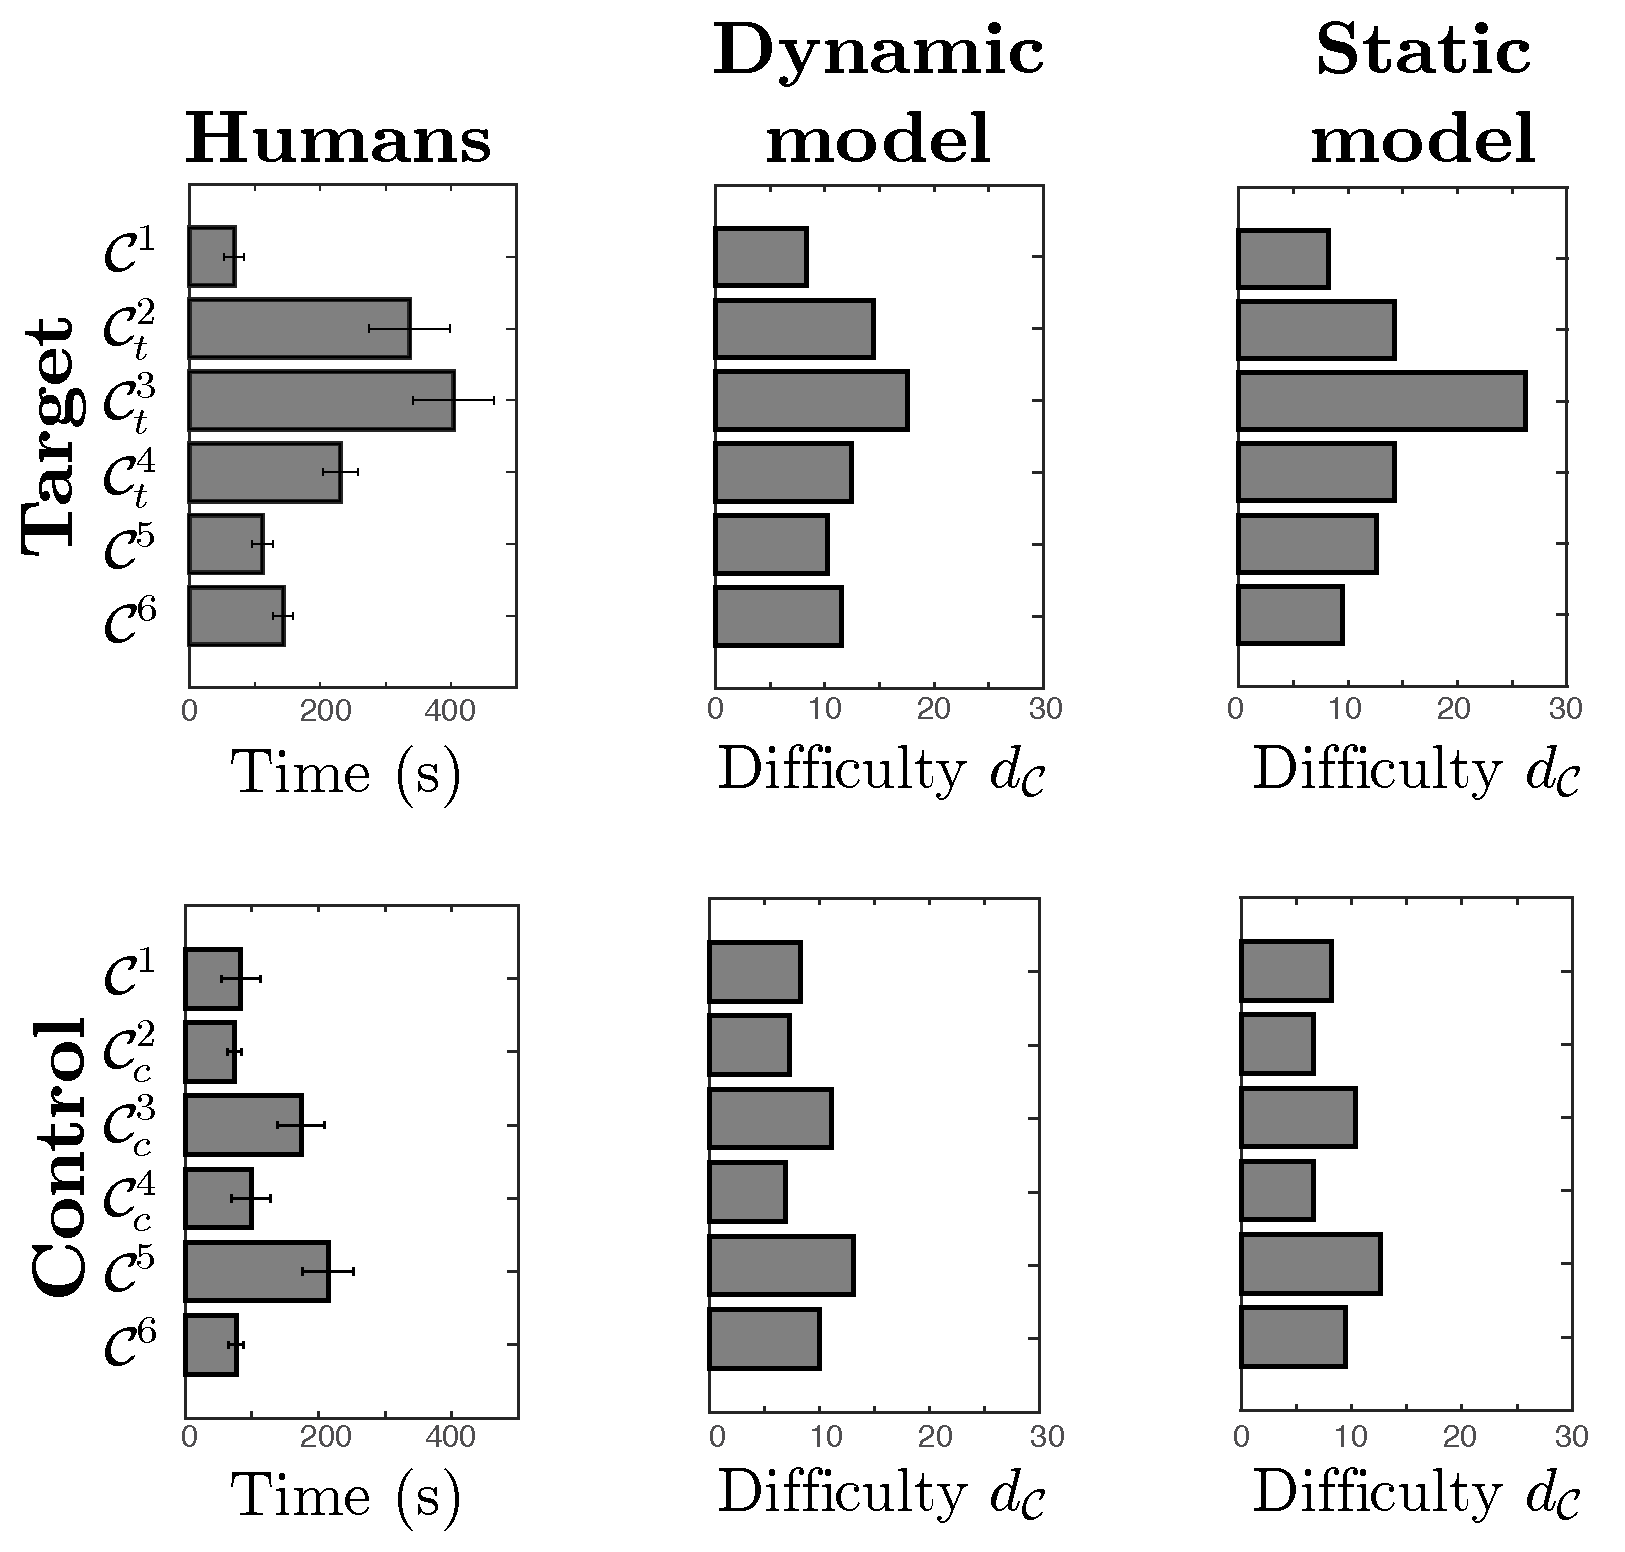
\includegraphics[scale=.45]{results-3.pdf}
      \caption{
      % Learning times and model predictions for target and control groups (see Table~\ref{conceptos} for concept details). The predicted difficulties of each model were calculated using $d_\con$. Error bars are s.e.m.
      Tiempos de aprendizaje y predicciones de modelos para grupos objetivo y control (consultar la Tabla~\ref{conceptos} para obtener detalles de los conceptos). Las dificultades predichas de cada modelo se calcularon utilizando $ d_\con $. Las barras de error son s.e.m.
      }
      \label{results}
\end{figure}

\begin{figure}
        \centering
        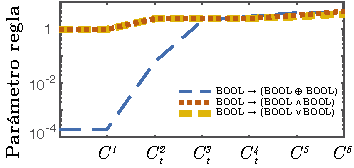
\includegraphics[scale=1.5]{dirichlet_evol-2.pdf}
        \caption{
        % Evolution of Dirichlet parameters of different rules after each concept experienced by the target group.
        Evolución de los parámetros de Dirichlet de diferentes reglas después de cada concepto experimentado por el grupo objetivo.
        }
       \label{evol}
\end{figure}

% However, the little increment in the $\oxor$ rule after \targetb (see Figura~\ref{evol}) is sufficient for making the formula $x_{k} \oxor x_{l}$ to have higher relative posterior in the next concepts, making the increment in the parameter of the $\oxor$ rule much greater than before. Additionally, the difficulty inferred by the model is much smaller the second time the concept is presented (compare \targetd and \targetb concepts in Figura~\ref{results}), since now the posterior is more evenly distributed between long (without $\oxor$) and short (with $\oxor$) formulas (see Eq. \eqref{expected length}). Finally, when the concept \testa is presented, the learner has completely compiled the $\oxor$ rule into her language, ascribing the formulas that use the $\oxor$ operator a much higher posterior probability relative to the long formulas that do not use the $\oxor$ operator. Therefore, the inferred difficulty for \testa is much smaller than those describing previous concepts, almost as simple as concept \targeta (see Figura~\ref{results}).
Sin embargo, el pequeño incremento en la regla $ \oxor $ después de \targetb (ver Figura~\Ref{evol}) es suficiente para hacer que la fórmula $x_ {k} \oxor x_{l} $ tenga una probabilidad a posteriori relativa más alta en los siguientes conceptos, haciendo que el incremento en el parámetro de la regla $ \oxor $ sea mucho mayor que antes. Además, la dificultad inferida por el modelo es mucho menor la segunda vez que se presenta el concepto (comparar los conceptos \targetd y \targetb en la Figura~\ref{results}), ya que ahora la probabilidad a posteriori se distribuye más uniformemente entre fórmulas largas (sin $ \oxor $) y fórmulas cortas (con $ \oxor $) (ver la ecuación \eqref{expected length}). Finalmente, cuando se presenta el concepto \testa, el aprendiz ha compilado completamente la regla $ \oxor $ en su lenguaje, atribuyendo a las fórmulas que usan el operador $ \oxor $ una probabilidad a posteriori mucho más alta en relación con las fórmulas largas que no usan el operador $ \oxor $. Por lo tanto, la dificultad inferida para \testa es mucho menor que las que describen los conceptos anteriores, casi tan simple como el concepto \targeta (ver Figura~\ref{results}).

% Finally, the strong $\oxor$ acquired by the target group increases the difficulty of \testb relative to the control group (see Figura 3). This occurs because there are several formulas of length 9 that use the $\oxor$ operator (around 6000), significantly increasing the expected difficulty of the concept (see Eq. \eqref{expected length}). For the control group, the posterior probability of these formulas is very low, causing a smaller increase in the expected difficulty.
Finalmente, la fuerte adquisición de $ \oxor $ por el grupo objetivo aumenta la dificultad de \testb en relación con el grupo de control (ver Figura~\ref{results}). Esto ocurre porque hay varias fórmulas de longitud $9$ que usan el operador $ \oxor $ (alrededor de $6000$), lo que aumenta significativamente la dificultad esperada del concepto (ver ecuación \eqref{expected length}). Para el grupo control, la probabilidad a posteriori de estas fórmulas es muy baja, provocando un menor aumento de la dificultad esperada.

% The previous results point to a competition between different rules in the grammar. In our model, competition between $\oxor$ and the other operators is modulated by the initial relative value of the Dirichlet prior of the $\oxor$ rule, and the overall magnitude of the priors of all rules. The initial $\oxor$ prior measures how useful $\oxor$ should be (relative to the other rules) in order to increase the likelihood of using it in the future. If the $\oxor$ prior is too low relative to the priors of other rules, then formulas with $\oxor$ must be much shorter than formulas without $\oxor$ in order for them to have appreciable posterior and increase the $\oxor$ parameter in Eq. \eqref{Dirichlet}. In our experiment, if the prior is smaller $10^{-12}$ (and 1 for all other rules), then the predictions of the dynamic and static model for the target group are approximately equal: the advantage of using $\oxor$ in the target concepts is not enough to increase the likelihood of using $\oxor$. On the other hand, if the $\oxor$ prior is too high, we cannot model the high difficulty of \targetb for the target group and the high difficulty of \testa for the control group. For example, if the $\oxor$ prior is higher than 0.05 (and 1 for all other rules), the difficulty of \targetb and \targetd are approximately equal (corresponding to the short formula with $\oxor$) and also the difficulties of \testa for control and target groups.
Los resultados anteriores apuntan a una competencia entre diferentes reglas en la gramática. En nuestro modelo, la competencia entre $ \oxor $ y los otros operadores está modulada por el valor relativo inicial de la probabilidad a priori de Dirichlet de la regla $ \oxor $ y la magnitud general de las distribuciones a priori de todas las reglas. La probabilidad a priori inicial del $ \oxor $ mide qué tan útil debería ser $ \oxor $ (en relación con las otras reglas) para aumentar la probabilidad de usarlo en el futuro. Si la probabilidad a priori de $ \oxor $ es demasiado baja en relación con las distribuciones a priori de las otras reglas, entonces las fórmulas con $ \oxor $ deben ser mucho más cortas que las fórmulas sin $ \oxor $ para que tengan una probabilidad a posteriori apreciable y aumenten el parámetro de $ \oxor $ en la ecuación~\eqref{Dirichlet}. En nuestro experimento, si el valor de la probabilidad a priori es menor $ 10^{- 12} $ (y $1$ para todas las demás reglas), entonces las predicciones del modelo dinámico y estático para el grupo objetivo son aproximadamente iguales: la ventaja de usar $ \oxor $ en los conceptos objetivos no es suficiente para aumentar la probabilidad de usar $ \oxor $. Por otro lado, si la probabilidad a priori de $ \oxor $ es demasiado alta, no podemos modelar la alta dificultad de \targetb para el grupo objetivo y la alta dificultad de \testa para el grupo de control. Por ejemplo, si la probabilidad a priori de $ \oxor $ es mayor que $0.05$ (y $1$ para todas las demás reglas), la dificultad de \targetb y \targetd son aproximadamente iguales (correspondientes a la fórmula corta con $ \oxor $) y también las dificultades de \testa para control y grupos objetivo. 

% The other free parameter that modulates competition is the overall magnitude of the Dirichlet priors, which determines how many times an efficient rule should be encountered before incorporating it. If the magnitude is too high, then observing a useful rule does not significantly change its Dirichlet parameter relative to the others, eliminating from the model the rapid rule acquisition clearly showed by participants. This happens because in Eq. \eqref{Dirichlet} the magnitude of the updates from $t$ to $t+1$ are at most of order $M$, the number of times that operators appear in formulas with high posterior. In our experiment, if all rules have prior equal to 1 and $\oxor$ has 1/1000 we get similar results to the ones in Figura~\ref{results}, but if all rules have prior equal to 10000 and $\oxor$ has 10 the additions to the $\oxor$ parameter are insignificant, so the dynamic and static models make the same predictions for the target group.
El otro parámetro libre que modula la competencia es la magnitud general de las probabilidades a priori de Dirichlet, que determina cuántas veces se debe encontrar una regla eficiente antes de incorporarla. Si la magnitud es demasiado alta, la observación de una regla útil no cambia significativamente su parámetro de Dirichlet en relación con los demás, eliminando del modelo la rápida adquisición de reglas claramente mostrada por los participantes. Esto sucede porque en la ecuación~\eqref{Dirichlet} la magnitud de las actualizaciones de $ t $ a $ t + 1 $ son como máximo del orden $ M $, el número de veces que los operadores aparecen en fórmulas con probabilidad a posteriori alta. En nuestro experimento, si todas las reglas tienen una probabilidad a priori igual a $1$ y $ \oxor $ tiene una de $1/1000$, obtenemos resultados similares a los de la Figura~\ref{results}, pero si todas las reglas tienen una probabilidad a priori igual a $10000$ y $ \oxor $ tiene $10$, las adiciones al parámetro de $ \oxor $ son insignificantes, por lo que los modelos dinámico y estático hacen las mismas predicciones para el grupo objetivo.

% In our model a large enough exposure to a concepts will increase the Dirichlet parameters without bounds, progressively decreasing learning flexibility. Although our experiment is not long enough to test it, such inflexibility is very unlikely to be true. For example, in the \lot fitting experiment from~\cite{piantadosi2016logical} they found that human Dirichlet priors for most propositional operators are between 0.3 and 3, instead of orders of magnitude higher (as expected by Eq. \eqref{Dirichlet} after exposure to a large number of concepts). Therefore, a more complete model of lifelong language acquisition should include an extra normalization or forgetting parameter that decreases the overall magnitude of the Dirichlet parameters, preserving the high learning flexibility that we observed in our experiment.
En nuestro modelo, una exposición suficientemente grande a conceptos aumentará los parámetros de Dirichlet sin límites, disminuyendo progresivamente la flexibilidad de aprendizaje. Aunque nuestro experimento no es lo suficientemente largo para probarlo, es poco probable que tal inflexibilidad sea cierta en las personas después de una larga exposición a conceptos. Por ejemplo, en el experimento de ajuste de \lot de~\cite{piantadosi2016logical} se encontró que las probabilidades a priori de Dirichlet para humanos para la mayoría de los operadores proposicionales están entre $0.3$ y $3$, en lugar de órdenes de magnitud más altos (como esperaba la ecuación~\eqref{Dirichlet} después de la exposición a una gran cantidad de conceptos). Por lo tanto, un modelo más completo de adquisición del lenguaje a lo largo de la vida debería incluir un parámetro extra de normalización u olvido que disminuya la magnitud general de los parámetros de Dirichlet, preservando la alta flexibilidad de aprendizaje que observamos en nuestro experimento.

% \section{Discussion}
\section{Discusión}

% \par We measured the subjective difficulty that participants experience when learning a sequence of concepts. To explain this subjective difficulty, we resource to propositional logic as a  base description language. In the target group we experimented with concepts which can be succinctly described in the base language {\em that also contains an extra operator $\oxor$} for exclusive disjunction but that needed necessarily longer descriptions over the base language (where this operator is absent). On the contrary, the control group is exposed to concepts where $\oxor$ does not help to achieve succinctness.
Medimos la dificultad subjetiva que experimentan los participantes al aprender una secuencia de conceptos. Para explicar esta dificultad subjetiva, recurrimos a la lógica proposicional como lenguaje de descripción base. En el grupo objetivo, experimentamos con conceptos que pueden describirse sucintamente en el lenguaje base {\em si se le agrega un operador adicional $ \oxor $} para la disyunción exclusiva pero que necesita descripciones más largas sobre el lenguaje base (donde este operador está ausente). Por el contrario, el grupo de control está expuesto a conceptos donde $ \oxor $ no ayuda a lograr descripciones más concisas.

% Learning times are consistent with the hypothesis that participants in the target group smoothly adopt the $\oxor$ as a new primitive of their \lot in order to absorb the concepts they have been exposed to, with no more incentive than decreasing the expected complexity of future concepts. We do not claim that participants have learned the $\oxor$ operator defined by any specific formula using the previous operators, however, their \lot seems to have constructed an operation that matches the semantics of the exclusive or in order to compress such patterns of data and identify them more efficiently.
Los tiempos de aprendizaje son consistentes con la hipótesis de que los participantes en el grupo objetivo adoptan sin problemas el $ \oxor $ como una nueva primitiva de su \lot para absorber los conceptos a los que han estado expuestos, sin más incentivo que disminuir la complejidad esperada de futuros conceptos. No afirmamos que los participantes hayan aprendido el operador $ \oxor $ definido por ninguna fórmula específica usando los operadores anteriores, sin embargo, su \lot parece haber construido una operación que coincide con la semántica de la disyunción exclusiva para comprimir tales patrones de datos e identificarlos de manera más eficiente.

% \par Here, we focus on transfer learning effects when learning sequential concepts that share the same hierarchical structure. We acknowledge, however, that several other transfer learning effects are present in human sequential logical concept learning, such as when subsequent concepts differ in the relevant variables (e.g.\  color lights in our experiment)~\cite{blair2009extremely}, when changing the relevant variables in subsequent exclusive disjunctions~\cite{kruschke1996dimensional}, or when two categories are learned in an interleaved or a focused manner~\cite{carvalho2014putting}. However, unlike superficial knowledge about the task (like the frequency of appearance of different symbols and logical operators in the concept sequence), identifying the latent hierarchical structure of concepts have extremely important computational consequences: it allows for exponentially less complex representations~\cite{bengio2013representation,lake2015human}, maximizing the expected value of future computations within resource-bounded constraints~\cite{gershman2015computational}. In our task, in order to focus primarily on the learning process of the $\oxor$ structure, we randomize variables in each trial, such that other kinds of transitions are averaged out across participants. 
Aquí, nos enfocamos en los efectos del aprendizaje de transferencia al aprender conceptos secuenciales que comparten la misma estructura jerárquica. Sin embargo, reconocemos que varios otros efectos del aprendizaje de transferencia están presentes en el aprendizaje secuencial de conceptos lógicos humanos, como cuando los conceptos posteriores difieren en las variables relevantes (por ejemplo, luces de color en nuestro experimento)~\cite{blair2009extremely}, al cambiar las variables relevantes  en disyunciones exclusivas subsecuentes~\cite{kruschke1996dimensional}, o cuando dos categorías se aprenden de forma intercalada o enfocada~\cite{carvalho2014putting}. Sin embargo, a diferencia del conocimiento superficial sobre la tarea (como la frecuencia de aparición de diferentes símbolos y operadores lógicos en la secuencia de conceptos), identificar la estructura jerárquica latente de los conceptos tiene consecuencias computacionales extremadamente importantes: permite representaciones exponencialmente menos complejas~\cite{bengio2013representation,lake2015human}, maximizando el valor esperado de cálculos futuros dentro de restricciones de recursos  limitados~\cite{gershman2015computational}. En nuestra tarea, para centrarnos principalmente en el proceso de aprendizaje de la estructura $ \oxor $, aleatorizamos las variables en cada ensayo, de modo que se promedien otros tipos de transiciones entre los participantes.

% \par Most \lot studies provide a language that is fixed once trained or inferred over a specific data. We claim that when a specific language beats a second one at fitting some experimental data, what we may be seeing is an effect of prior experience (including from the experiment itself), more than an intrinsic feature of the \lot. This leads to a fundamental difficulty in trying to experimentally uncover what the actual human symbolic substrate of thought is. Experimental results have shown for instance that a grammar with \textit{and, or}, and \textit{not} better explains Boolean concept learning than one with \textit{nand}, despite both being expressively equivalent~\cite{piantadosi2016logical}.  In our view, this cannot be taken to mean anything more than that in the current state of affairs of the world, the \textit{nand} operator is not very useful for compressing information. We have shown that participants can rapidly compile new expressions in their \lot if they begin to be useful, which emphasizes that one cannot simply ignore the order in which concepts are presented to the participant when studying aspects of the \lot.
La mayoría de los estudios de \lot proporcionan un lenguaje fijo una vez que se entrena o se infiere sobre datos específicos. Afirmamos que cuando un lenguaje específico supera a otro en el ajuste de algunos datos experimentales, lo que podemos estar viendo es un efecto de la experiencia previa (incluso del experimento en sí), más que una característica intrínseca del \lot. Esto conduce a una dificultad fundamental para tratar de descubrir experimentalmente cuál es el sustrato simbólico humano real del pensamiento. Los resultados experimentales han demostrado, por ejemplo, que una gramática con \textit{y}, \textit{o}, y \textit{no} explica mejor el aprendizaje de conceptos booleanos que una con \textit{nand}, a pesar de que ambas son expresivamente equivalentes~\cite{piantadosi2016logical}. En nuestra opinión, esto no puede significar nada más que el hecho de que en el estado actual de las cosas del mundo, el operador \textit{nand} no es muy útil para comprimir información. Hemos demostrado que los participantes pueden compilar rápidamente nuevas expresiones en su \lot si comienzan a ser útiles, lo que enfatiza que no se puede simplemente ignorar el orden en el que se presentan los conceptos al participante cuando se estudian aspectos de la \lot.

% When Fodor proposed the Language of Thought hypothesis~\cite{fodor1975language}, what he had in mind was a symbolic system we all came equipped with from birth. Stating that this language is in fact always flexible might seem in outright contradiction with Fodor's original idea. In fact, what studies in the \lot literature (including this one) are probably probing is one among many languages in a hierarchy of increasing abstraction. As we progress in life, we find some conceptual summaries useful, and compiled them in a more abstract token. It is even likely that there is no proper hierarchy with sharply defined boundaries between levels, but instead a less organized progression of concepts of increasing abstraction, with thought progressing seamlessly using constructs at different levels. he way for a broader understanding of human cognition.
Cuando Fodor propuso la hipótesis del lenguaje del pensamiento~\cite{fodor1975language}, lo que tenía en mente era un sistema simbólico con el que todos venimos equipados desde que nacimos. Afirmar que este lenguaje es siempre flexible puede parecer una contradicción con la idea original de Fodor. De hecho, lo que probablemente están investigando los estudios en la literatura de \lot (incluido este) es uno entre muchos lenguajes en una jerarquía de abstracción creciente. A medida que avanzamos en la vida, encontramos útiles algunos resúmenes conceptuales y los compilamos o encapsulamos en una pieza más abstracta. Incluso es probable que no exista una jerarquía adecuada con límites claramente definidos entre niveles, sino una progresión menos organizada de conceptos de creciente abstracción, en donde el pensamiento progresa sin problemas utilizando construcciones en diferentes niveles.

% \section{Conclusion}
%\section{Conclusiones}

% We defined a model to measure the subjective difficulty of learning a sequence of concepts. The model updates the grammar production probabilities between concepts and predicts difficulty as the size of compatible formulas weighted by their posterior probability. This learning mechanism allows to simulate the emergence of a new primitive in the language, as it becomes useful to encode the concepts presented so far. The predicted difficulties strongly resembles the pattern of human learning times in a sequence of concepts that required the $\oxor$ operator in order to be efficiently represented.

    %!TEX root = ../main.tex


\chapter{Un marco lógico para estudiar aprendizaje de conceptos en presencia de explicaciones múltiples}\label{chapter:BRM}
\chaptermark{Un marco lógico para explicaciones múltiples}




\section{Introducción}

% Concept acquisition is a key and widely studied aspect of human daily cognition~\cite{cohen2005handbook, ashby2011human}. Many researchers have claimed that a coding system and a set of rules underlie some of our  abilities to acquire concepts~\cite{nosofsky1994rule,tenenbaum2011grow,maddox1993comparing}, and it has been observed that we seem to learn concepts of objects with more ease when there are `simpler' rules that can explain those groupings~\cite{shepard1961learning, nosofsky1994comparing, rehder2005eyetracking, lewandowsky2011working,feldman2000minimization,blair2003easy,minda2001prototypes}. 

%La adquisición de conceptos es un aspecto clave y ampliamente estudiado de la cognición diaria humana~\cite{cohen2005handbook, ashby2011human}. Muchos investigadores han afirmado que un sistema de codificación y un conjunto de reglas subyacen a algunas de nuestras habilidades para adquirir conceptos~\cite{nosofsky1994rule, tenenbaum2011grow, maddox1993comparing}, y se ha observado que parece que aprendemos conceptos de objetos con más facilidad cuando hay reglas `más simples' que pueden explicar esas agrupaciones~\cite{shepard1961learning, nosofsky1994comparing, rehder2005eyetracking, lewandowsky2011working, feldman2000minimization, blair2003easy, minda2001prototypes}.

% In the real-world, humans learn concept descriptions while simultaneously deciding on which features to attend~\cite{schyns1998development}; and the selected set of features usually determines the structure and complexity of the minimal rules that can describe the concept. For example, the concept \textit{dog} can be explained as {\em a four-legged pet that is not a cat} or as {\em an animal for hunting, herding, pulling sledges or company}. Both descriptions are fully compatible with the concept \textit{dog}, but our experience induces us to choose different relevant features to define the concept. While the first description of {\em dog} could be very well be given by a child having a dog at home, the second could be given by a shepherd or perhaps an ethologist. It is likely that the features used to describe {\em dog} by each agent allows them to compactly describe the concept, while simultaneously separating it from other concepts frequently encountered in their environment. Here, we ask about which features participants use to describe concepts, depending on the logical structure of the description using those features and also on their exposure to previous concepts. Why will someone use {\em cat} or {\em hunting} to define {\em dog}?

La adquisición de conceptos es un aspecto clave y ampliamente estudiado de la cognición  humana~\cite{cohen2005handbook, ashby2011human}. En el proceso de aprender las descripciones de los conceptos, los humanos deciden simultáneamente a qué características atender~\cite{schyns1998development}; y el conjunto de características seleccionado generalmente determina la estructura y complejidad de las reglas que pueden describir el concepto. Por ejemplo, el concepto \textit{perro} se puede explicar como {\em una mascota de cuatro patas que no es un gato} o como {\em un animal para caza, pastoreo, tira de trineos o compañía}. Ambas descripciones son totalmente compatibles con el concepto \textit{perro}, pero nuestra experiencia nos induce a elegir diferentes características relevantes para definir el concepto. Mientras que la primera descripción de {\em perro} podría perfectamente haber sido dada por un niño que tiene un perro en la casa, la segunda podría haber sido presentada por un pastor o quizás un etólogo. Es probable que las características utilizadas para describir {\em perro} por cada agente les permitan describir de manera compacta el concepto, al mismo tiempo que lo separan de otros conceptos que se encuentran con frecuencia en su entorno. En este capítulo, nos preguntamos qué características usan los humanos para describir conceptos, dependiendo de la estructura lógica de la descripción que usa esas características y también de su exposición a conceptos anteriores. ¿Por qué alguien usaría {\em gato} o {\em caza} para definir {\em perro}?

\begin{figure}[h!]
\begin{center}
% 	\includegraphics[scale=.6]{../figuras/brm/intro_notation.pdf}
% \end{center}\caption{Illustration of the features $\{p_1,p_2,p_3,p_4\}$, the example $(1,1,0,1)$, and a concept (positive example are marked with bold boundaries and negative examples with thin boundaries). The concept can be explained with the two minimal rules $p_1 \land p_2$ or $p_3 \lor p_4$, depending on which features are used to build the rule (the first two features or the last two features, respectively).}
	\includegraphics[scale=.6]{../figuras/brm/intro_notation_sp.pdf}
\end{center}\caption{Ilustración de las características $\{p_1,p_2,p_3,p_4\}$, el ejemplo $(1,1,0,1)$, y un concepto (los ejemplos positivos están marcados con bordes gruesos y los ejemplos negativos con bordes delgados). El concepto se puede explicar con las dos reglas mínimas $p_1 \land p_2$ o $ p_3 \lor p_4$, dependiendo de las características que se usen para construir la regla (las dos primeras características o las dos últimas características, respectivamente). {\em Cf.}~Figura~\ref{semaforos}: en este caso el concepto ilustrado es parcial o {\em indeterminado}, en el sentido de que no todas las valuaciones posibles aparecen como positivas o negativas, en cambio, en la Figura~\ref{semaforos}, el concepto es completo, tal como fue definido formalmente al principio de la parte~\ref{parte:conceptos}.}
\label{fig:intro_notation}
\end{figure}


% In propositional concept-learning experiments, participants are presented with a set of \textit{examples}, each conformed of $N$ propositional \textit{features}, which can take positive or negative values. For instance, for $N=4$ one example can be logically represented as the element $(1,1,0,1)$, which takes positive values for the first, second and fourth features and negative for the second one, as illustrated in Figure~\ref{fig:intro_notation}. A \textit{concept} can be intuitively understood as a set of examples, some of them marked as belonging to the concept and the rest marked as not belonging, i.e.\ positive and negative examples. In Figure~\ref{fig:intro_notation} we show an example of an \textit{underdetermined} concept, in the sense that, since the entire universe of examples is not shown (i.e. the $2^4$ possibilities), different determined concepts can be consistent with this smaller set when extending the set of examples to the full universe. 
En los experimentos de aprendizaje de conceptos proposicionales, a los participantes se les presenta un conjunto de \textit{ejemplos}, cada uno conformado por $N$ \textit{características} proposicionales, que pueden tomar valores positivos o negativos, como se explicó al principio de la Parte~\ref{parte:conceptos}. Por ejemplo, para $N=4$ un {\em ejemplo} se puede representar lógicamente como el elemento $(1,1,0,1)$, que toma valores positivos para la primera, segunda y cuarta características y negativos para la segunda, como ilustramos en la Figura ~\ref{fig:intro_notation}. Como puede verse en la figura mencionada, elegimos para este capítulo una representación de las valuaciones distinta a la elegida en el Capítulo~\ref{chapter:PRE} (para más detalles, ver sección~\ref{Experiment_design}). Como sabemos, un \textit{concepto} puede entenderse intuitivamente como un conjunto de ejemplos, algunos de ellos marcados como pertenecientes al concepto y el resto marcados como no pertenecientes, es decir, ejemplos positivos y negativos. En la Figura~\ref{fig:intro_notation} mostramos un ejemplo de un concepto \textit{subdeterminado}, en el sentido de que, dado que no se muestra universo completo de ejemplos (es decir, las $2^4$ posibilidades), diferentes conceptos determinados pueden ser coherentes con este conjunto más pequeño al extender el conjunto de ejemplos al universo completo.


% A \textit{rule} consistent with the concept is a logical formula built with the features and the conjunction ($\land$), disjunction ($\lor$), and negation ($\lnot$) operators, which evaluates to true for objects belonging to the concept and false otherwise (e.g.\ $p_1 \land p_2$, where $p_i$ is the $i^{th}$ feature, see Figure~\ref{fig:intro_notation}). The \textit{minimal description length} (\textit{MDL}) of a concept is the length of the shortest rule consistent with the concept~\cite{grunwald2007minimum} (here, the {\em length} of a formula is defined as the number of positive or negative occurrences of propositional symbols plus the number of occurrences of operators $\land$ or $\lor$ contained in it; for example, the length of $p_1 \land \lnot p_3$ is 3, and the length of $(p_1 \land \lnot p_3)\lor p_2$ is 5). Importantly, most studies of subjective difficulty with concept-learning are designed such that a {\em single} minimal rule can be used to describe the concept (e.g.\ $p_1 \land p_2$)~\cite{ashby2005human,feldman2000minimization}, even when the difficulty of finding the features that compose that rule ($p_1$ and $p_2$) is measured with attention-tracking mechanisms (e.g.\~\cite{blair2009extremely,hoffman2010costs}). This limitation is possibly due to the prohibitively large number of rules that can be built with a given set of features, making it difficult to control which rules the participant might use when observing a set of examples. For instance, in order to determine the difficulty that participants have in learning the logical rule $p_1 \lor p_2$, it is crucial to control that no other rule of reasonable complexity can explain the concept (e.g.\ $p_1 \land p_3$). In this work, we use the tools of propositional logic to build an experimental framework that allows us to present examples consistent with two (or more) chosen rules, depending on which features are observed. For instance, the concept shown in Figure~\ref{fig:intro_notation} is consistent with the explanation $p_1 \land p_2$ \textit{and also} with the explanation $p_3 \lor p_4$, depending on which features are observed. In general, the experimenter can choose any pair of rules that use any number of (non-overlapping) features, and our framework guarantees that the presented examples are only consistent with the two minimal rules chosen by the experimenter. Then, by presenting novel examples that are consistent with only one of the previous rules, the experimenter can determine which rule the participants internally used to learn the concept, and thus which features they attended to.

Utilizaremos también en este capítulo la gramática \grambool, junto a su semántica y medida de complejidad, \mdlbool, tal cual la hemos definido al inicio de la Parte II. Es importante destacar que la mayoría de los estudios sobre la dificultad subjetiva en el aprendizaje de conceptos están diseñados de manera que se pueda usar una {\em única} regla mínima para describir el concepto (por ejemplo, $p_1 \land p_2$)~\cite{ashby2005human,feldman2000minimization}, incluso cuando la dificultad de encontrar las características que componen esa regla ($p_1$ y $p_2$) se mide con mecanismos de seguimiento de atención (por ejemplo,~\cite{blair2009extremely, hoffman2010costs}). Esta limitación se debe posiblemente a la cantidad prohibitivamente grande de reglas que se pueden construir con un conjunto de características dado, lo que dificulta el control de las reglas que el participante podría usar al observar un conjunto de ejemplos que representan parcialmente a un concepto. Por caso, para determinar la dificultad que tienen los participantes en aprender la regla lógica $p_1 \lor p_2$, es crucial controlar que ninguna otra regla de complejidad razonable pueda explicar el concepto (por ejemplo, $p_1 \land p_3$). En este capítulo, utilizamos las herramientas de la lógica proposicional para construir un marco experimental que nos permita presentar ejemplos consistentes con dos (o más) reglas elegidas, dependiendo de qué características se observen. Por ejemplo, el concepto mostrado en la Figura~\ref{fig:intro_notation} es consistente con la explicación $p_1 \land p_2$ \textit {y también} con la explicación $p_3 \lor p_4$, dependiendo de qué características se observen. En general, el experimentador puede elegir cualquier par de reglas que usen cualquier número de características (no superpuestas), y nuestro marco garantiza que los ejemplos presentados solo son consistentes con las dos reglas mínimas elegidas por el experimentador. Luego, al presentar ejemplos novedosos que sean consistentes con solo una de las reglas anteriores, el experimentador puede determinar qué regla usaron los participantes internamente para aprender el concepto y, por lo tanto, a qué características prestaron atención.


% Presenting rules $A$ and $B$ (e.g.\ $p_1 \land p_2$ and $p_3 \lor p_4$) using the same set of examples has several experimental advantages over separately presenting a set of examples consistent with rule $A$ and then a set of examples consistent with rule $B$. Some of the advantages are: 
Presentar las reglas $A$ y $B$ (por ejemplo, $p_1\land p_2$ y $p_3 \lor p_4$) utilizando el mismo conjunto de ejemplos tiene varias ventajas experimentales sobre la presentación por separado de un conjunto de ejemplos coherentes con la regla $A$ y luego un conjunto de ejemplos consistentes con la regla $B$. Algunas de las ventajas son:

\begin{enumerate}
\item [(1)] 
% When comparing the relative difficulty of learning $A$ and $B$ in the same participant, presenting the examples separately makes it hard to overcome transfer effects that cause subjective difficulty to depend on the history of concepts learnt previously in the task, and cause different relative difficulties if $A$ is learnt before $B$ compared to $B$ being learnt before $A$ (see for example~\cite{tano2020towards}). The experimenter could compare learning times for $A$ and $B$ across participants, but for reasonably hard rules there are very large idiosyncratic differences in learning difficulties which greatly increases the variance of learning times (see for example~\cite{feldman2000minimization}), and also the experimenter cannot normalize the past history of each participant before the experiment. On the other hand, presenting $A$ and $B$ simultaneously via the same set of examples allows us to directly measure which of the two rules is most easily found by the participant, when the two are presented under exactly the same experimental conditions.
Cuando comparamos la dificultad relativa de aprender $A$ y $B$ en el mismo participante, si presentamos los ejemplos por separado, se complica superar los efectos de transferencia que hacen que la dificultad subjetiva dependa de la historia de conceptos aprendidos previamente en la tarea, y provoquen diferentes dificultades relativas si $A$ se aprende antes de $B$ en comparación a si $B$ se aprende antes de $A$ (ver por ejemplo~\cite{tano2020towards}). El experimentador podría comparar los tiempos de aprendizaje para $A$ y $B$ entre los participantes, pero para reglas razonablemente difíciles, existen diferencias idiosincrásicas muy grandes en las dificultades de aprendizaje que aumentan enormemente la variación de los tiempos de aprendizaje (ver, por ejemplo,~\cite{feldman2000minimization}). Además, el experimentador no puede normalizar la historia pasada de cada participante antes del experimento. Por otro lado, presentar $A$ y $B$ simultáneamente a través del mismo conjunto de ejemplos nos permite medir directamente cuál de las dos reglas encuentra más fácilmente el participante, cuando las dos se presentan exactamente bajo las mismas condiciones experimentales.

\item [(2)] 
% The fact that rule $A$ is learnt more easily than $B$ when presented separately does not necessarily mean that the same happens when presented jointly. This could not hold if there is an interaction between the logical operators being learnt (that compose the rules $A$ and $B$) and the search mechanism used to find the corresponding rules. For instance, the search mechanism that allows humans to find a disjunction rule consistent with the examples could interact with the mechanism that allows to find conjunctions, an interaction that could only be characterized when the conjunction and disjunction are presented at the same time.
El hecho de que la regla $A$ se aprenda más fácilmente que $B$ cuando se presentan por separado no significa necesariamente que suceda lo mismo cuando se presenta en conjunto. Esto podría no ser válido si existiera una interacción entre los operadores lógicos que se están aprendiendo (que componen las reglas $A$ y $B$) y el mecanismo de búsqueda utilizado para encontrar las reglas correspondientes. Por ejemplo, el mecanismo de búsqueda que permite a los humanos encontrar una regla de disyunción consistente con los ejemplos podría interactuar con el mecanismo que permite encontrar conjunciones, interacción que solo podría caracterizarse cuando la conjunción y la disyunción se presentan al mismo tiempo.

\item [(3)] 
% Our framework allows us to test second-order subjective difficulty effects (e.g.\ rule $A$ is learnt faster if presented jointly with rule $B$ than with rule $C$), as well as second-order transfer learning effects (e.g.\  participants learn more rapidly rule $C$ if they have first observed rule $A$ jointly presented with an arbitrary rule $B_1$, compared to $A$ coupled with a different rule $B_2$).
Nuestro marco nos permite probar efectos de dificultad subjetiva de segundo orden (por ejemplo, la regla $A$ se aprende más rápido si se presenta junto con la regla $B$ que si se presenta junto con la regla $C$), así como efectos de aprendizaje de transferencia de segundo orden (por ejemplo, los participantes aprenden más rápidamente la regla $C$ si primero han observado la regla $A$ presentada conjuntamente con una regla arbitraria $B_1$, en comparación con $A$ junto con una regla diferente $B_2$).

\item [(4)] 
% If one is interested in which features are preferentially observed by the participant in a given trial (e.g.\  features $\{p_1,p_2\}$ or $\{p_3,p_4\}$), one could simply choose the same logical structure for $A$ and $B$ (e.g.\ making $A$ and $B$ equal to $p_1 \land p_2$ and $p_3 \land p_4$) and test whether $A$ or $B$ is learnt by the participant. Then, any preference for learning $A$ over $B$ could only be due to a preference over the features themselves ($\{p_1,p_2\}$), and not for the logical description of the concept using those features (this is, $\boldsymbol{\cdot} \land \boldsymbol{\cdot}$).
Si uno está interesado en qué características observa preferentemente el participante en una prueba determinada (por ejemplo, las características $\{p_1, p_2 \}$ o $\{p_3, p_4 \} $), simplemente se podría elegir la misma estructura lógica para $A$ y $B$ (por ejemplo, haciendo que $A$ y $B$ sean iguales a $p_1 \land p_2$ y $p_3 \land p_4 $ respectivamente) y comprobar si el participante aprende $A$ o $B$. Entonces, cualquier preferencia por aprender $A$ sobre $B$ solo podría deberse a una preferencia sobre las características en sí mismas ($\{p_1, p_2 \} $), y no por la descripción lógica del concepto que usa esas características (esto es, $\boldsymbol{\cdot} \land \boldsymbol{\cdot}$).
\end{enumerate}



% We illustrate these advantages in an experiment in which participants are presented with a sequence of 6 trials, observing in each trial a set of examples consistent with two alternative rules. We illustrate advantage (1) and (2) discussed above by presenting a conjunction together with a disjunction; and a simple rule together with a complex rule. Then, we show that after observing in several trials that a subset of features is useful to find concise rules, we induce  in the participants a bias to preferentially describe concepts using those features; this bias was tested exploiting  advantage (4).
Ilustramos estas ventajas en un experimento en el que a los participantes se les presenta una secuencia de 6 pruebas, observando en cada prueba un conjunto de ejemplos consistentes con dos reglas alternativas. Ilustramos la ventaja (1) y (2) discutida anteriormente presentando una conjunción junto con una disyunción; y una regla simple junto con una regla compleja. Luego, mostramos que después de observar en varias pruebas que un subconjunto de características es útil para encontrar reglas concisas, inducimos en los participantes un sesgo para describir conceptos usando preferentemente esas características; este sesgo se testeó aprovechando la ventaja (4).






\section{Experimento}\label{Section:Experiment}
\subsection{Participantes} \label{Participants}

% The experiment was conducted as a Human Intelligence Task (HIT) in Amazon's Mechanical Turk~\cite{crump2013evaluating, buhrmester2011amazon, stewart2015average}. There were 100 participants,  self-selected workers that saw, accepted, and finished the published HIT. We required workers to have a HIT approval rate of $95\%$ or more. Workers were informed that the payment for completing the experiment was going to be of {1.5} US dollars, and that 1 out of 20 participants would be randomly assigned a bonus of 10 dollars, regardless of their performance in the experiment's tasks as long as they finished the experiment (but note that trials did not end until they correctly learned each concept).
Tal como el experimento del Capítulo~\ref{chapter:PRE}, el experimento que ahora describimos se llevó a cabo como una tarea de Human Intelligence Task (HIT) en Mechanical Turk~\cite{crump2013evaluating, buhrmester2011amazon, stewart2015average} de Amazon. Hubo 100 participantes, trabajadores autoseleccionados que vieron, aceptaron y terminaron el HIT publicado. Requerimos que los trabajadores tuvieran una tasa de aprobación HIT de $95 \%$ o más. Se informó a los trabajadores que el pago por completar el experimento sería de {1,5} dólares estadounidenses,
y que a 1 de cada 20 participantes se le asignaría aleatoriamente una bonificación de 10 dólares, independientemente de su desempeño en las tareas del experimento, siempre que terminaran el experimento (pero tener en cuenta que las pruebas no terminaron hasta que aprendieron correctamente cada concepto).

% For exclusion criteria, see the appendix~\S\ref{Sec:ExclusionCriteria}.
Para conocer los criterios de exclusión, consultar~\S\ref{Sec:ExclusionCriteria}.


\subsection{Configuración del experimento}\label{Subsec:ExperimentFlow}
% The main idea of our experimental framework is schematized in Figure~\ref{fig:twoconcepts}. The participants observe an \textit{underdetermined} concept. This concept is presented to the participants as a set of elements that belong to it (positive examples), and a set of elements that do not (negative examples). In  Figure~\ref{fig:twoconcepts}, the elements marked as positive examples are the ones in the intersection of the two concepts and the negative examples are the ones outside of both concepts. Importantly, the listing is incomplete, in the sense that not all elements of the universe are shown. The critical insight is that, when extending the set of examples to the full universe, there is more than one possible concept that is consistent with the observed examples.  For example, in Figure~\ref{fig:twoconcepts},  the presented examples are consistent with the minimal rule of $C_1$ (i.e.\ $\varphi_1=p_1\lor p_2$) \textit{and also} with the minimal rule of $C_2$ (i.e.\ $\varphi_2=p_3\land p_4$). As we explain in the rest of this section, choosing $C_1$ and $C_2$ appropriately can be exploited to control the minimal rules that are consistent with the examples that participants observe.
La idea principal de nuestro marco experimental se esquematiza en la Figura~\ref{fig:twoconcepts}. Los participantes observan un concepto \textit{indeterminado}. Este concepto se presenta a los participantes como un conjunto de elementos que le pertenecen (ejemplos positivos), y un conjunto de elementos que no (ejemplos negativos). En la Figura~\ref{fig:twoconcepts}, los elementos marcados como ejemplos positivos son los que están en la intersección de los dos conceptos y los ejemplos negativos son los que están fuera de ambos conceptos. Es importante destacar que la lista es incompleta, en el sentido de que no se muestran todos los elementos del universo, es decir, todas las valuaciones posibles (como era el caso del experimento del Capítulo~\ref{chapter:PRE}). La idea fundamental es que, al extender el conjunto de ejemplos al universo completo, hay más de un concepto posible que es consistente con los ejemplos observados. Por ejemplo, en la Figura~\ref{fig:twoconcepts}, los ejemplos presentados son consistentes con la regla mínima de $C_1$ (es decir, $\varphi_1 = p_1 \lor p_2$) \textit {y también} con la regla mínima de $C_2$ (es decir, $\varphi_2 = p_3 \land p_4$). Como explicamos en el resto de esta sección, la elección adecuada de $C_1$ y $C_2$ puede aprovecharse para controlar las reglas mínimas que son consistentes con los ejemplos que observan los participantes.


\begin{figure}[h!]
\begin{center}
	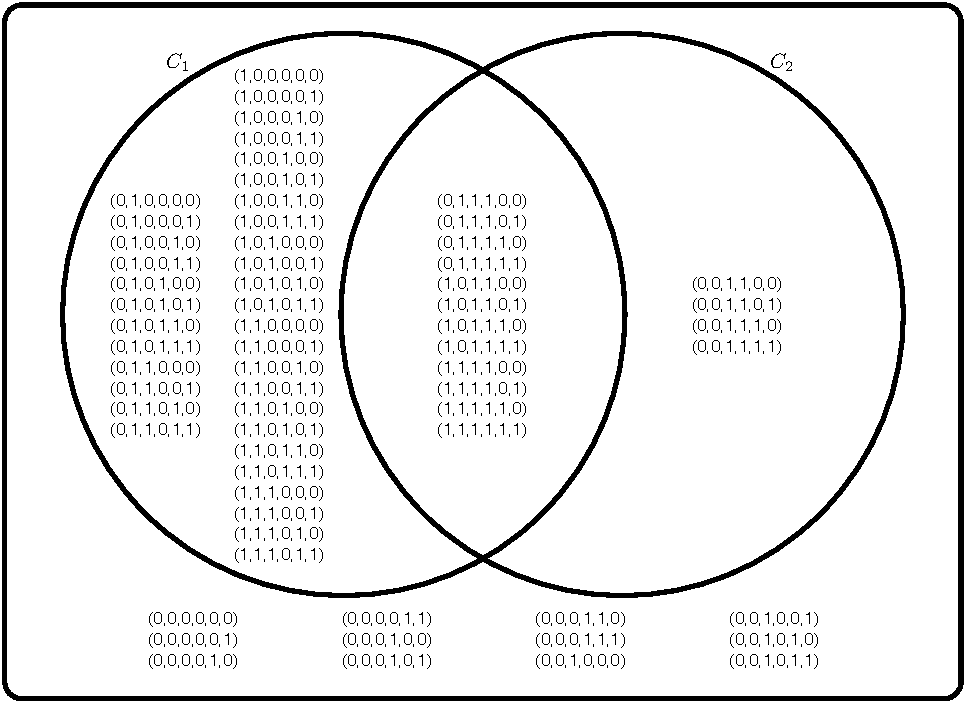
\includegraphics[scale=.65]{../figuras/brm/twoconcepts3.pdf}
\end{center}\caption{
%An example of a pair of concepts $C_1$ and $C_2$ with 6 features. Concept $C_1$ can be described by $\varphi_1=p_1 \lor p_2$, and $C_2$ by $\varphi_2=p_3\land p_4$. This is just a schematic illustration of where each element (tuple) is placed with respect to concepts. These concepts correspond to the ones used in Trial 1 of the actual experiment. However, elements in the actual experiment are not represented in this way (i.e.\ as tuples of zeroes and ones).
Un ejemplo de un par de conceptos $C_1$ y $C_2$ con 6 características. El concepto $C_1$ puede ser descrito por $\varphi_1 = p_1 \lor p_2 $, y $C_2$ por $\varphi_2 = p_3 \land p_4$. Esta es solo una ilustración esquemática de dónde se coloca cada elemento (tupla) con respecto a los conceptos. Estos conceptos corresponden a los utilizados en la Prueba 1 del experimento real. Sin embargo, los elementos del experimento real no se representan de esta manera (es decir, como tuplas de ceros y unos).
}
\label{fig:twoconcepts}
\end{figure} 

% The actual experiment that we implemented consists of a sequence of 6 trials constructed in this manner. We now expand the 3 stages that compose each $i$-th trial of the experiment. For a better understanding, see Figure~\ref{fig:trials}, which consists of a schematic view of one trial. Note that this figure is merely illustrative and does not aim to describe the details of a trial, but rather the sequence of phases and the logical flow within a trial. In particular, note that the number of elements {\sf A}'s, {\sf B}'s, {\sf C}'s and {\sf D}'s in the figure are not meaningful, as they vary from trial to trial along the experiment. The actual concepts used in each trial, as well as the number of positive and negative examples is listed in Table~\ref{trial_table} (groups X,Y are only relevant for Hypothesis III, so they can be ignored for now), and more details of the actual implementation can be found in \S\ref{sub:experimentdetails} and \S\ref{FullExperimentDescription}.
El experimento real que implementamos consiste en una secuencia de 6 pruebas, cada una de las cuales está construida de la manera que acabamos de describir. Tiene algunas semejanzas con el experimento descripto en el Capítulo~\ref{chapter:PRE} respecto al flujo lógico, pero  diferencias sustanciales que permiten responder la pregunta abordada en este capítulo. Ahora expandimos las 3 etapas que componen la $i$-ésima prueba del experimento. Para una mejor comprensión, consultar la Figura~\ref{fig:trials}, que consiste en una vista esquemática de una prueba. Tener en cuenta que esta figura es meramente ilustrativa y no pretende describir los detalles de una prueba, sino más bien la secuencia de fases y el flujo lógico dentro de una prueba. En particular, tener en cuenta que el número de elementos {\sf A}, {\sf B}, {\sf C} y {\sf D} en la figura no son significativos, ya que varían de prueba en prueba a lo largo del experimento. Los conceptos reales utilizados en cada ensayo, así como el número de ejemplos positivos y negativos se enumeran en la Tabla~\ref{trial_table} (los grupos X, Y solo son relevantes para la Hipótesis \ref{Hip:FeatureBiasTimeAdvantage}, por lo que pueden ignorarse por ahora), y se pueden encontrar más detalles de la implementación real en \S\ref{sub:experimentdetails} y \S\ref{FullExperimentDescription}.  
%
\begin{figure}[h!]
\begin{center}
	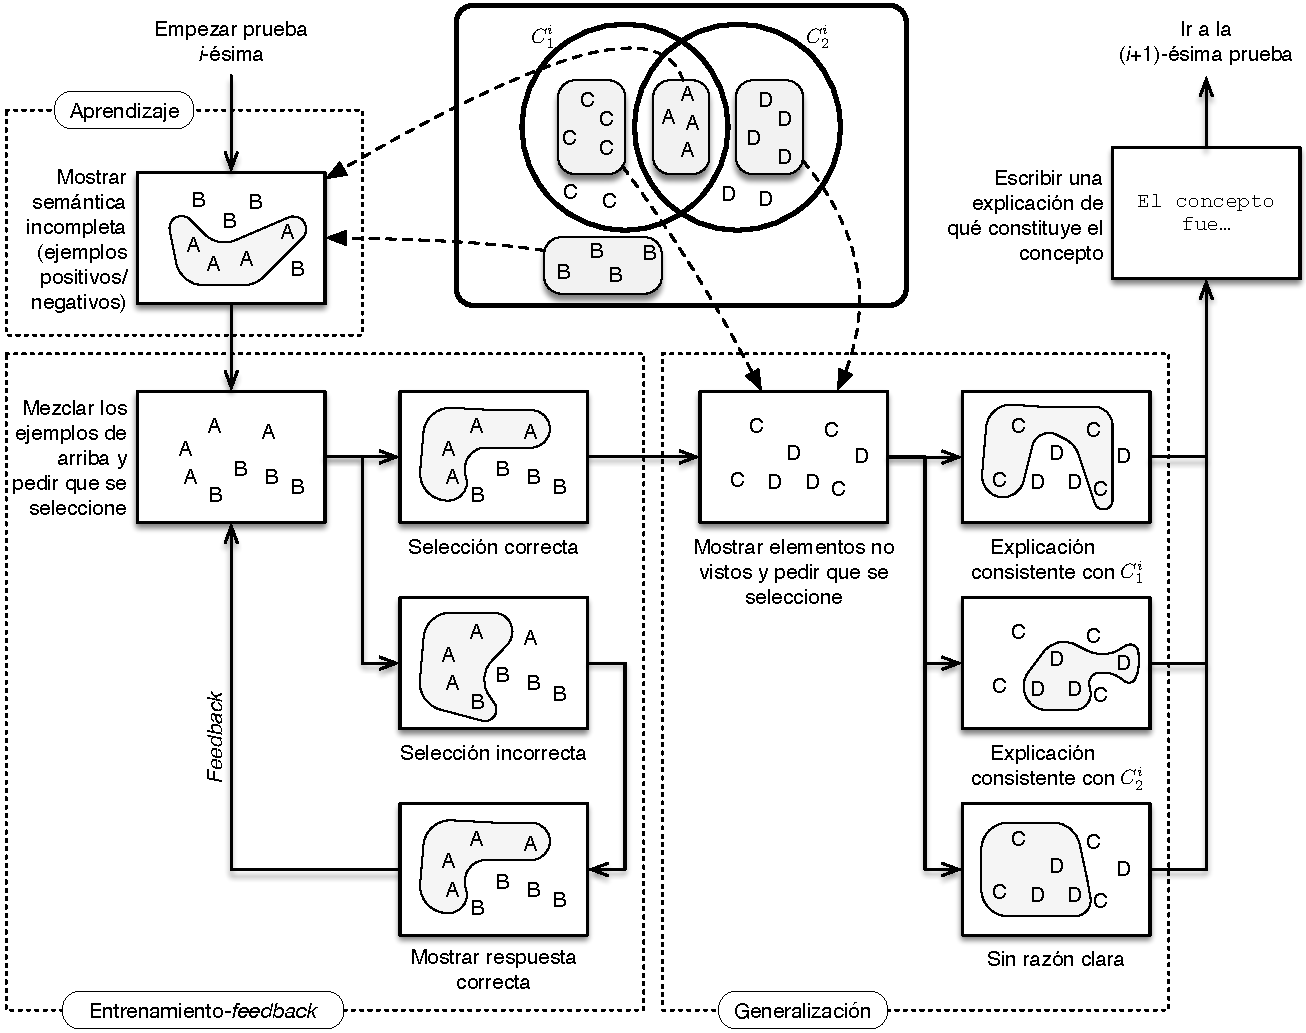
\includegraphics[scale=.7]{../figuras/brm/experimentscheme2_sp.pdf}
\end{center}\caption{
% The scheme of our experimental framework for studying concept learning in the presence of multiple explanations. We illustrate the three phases that constitute each trial: learning phase, training-feedback phase and generalization phase. Elements are represented with letters {\sf A}, {\sf B}, {\sf C} and {\sf D} (for example, the four letters {\sf A} in the intersection represent four different elements in the intersection). The depicted number of such letters {\sf A}, {\sf B}, {\sf C} or {\sf D} is irrelevant (for example, there would be 12 {\sf A}s and 4 {\sf D}s for concepts of Figure~\ref{fig:twoconcepts}).
El esquema de nuestro marco experimental para estudiar el aprendizaje de conceptos en presencia de múltiples explicaciones. Ilustramos las tres fases que constituyen cada ensayo: fase de aprendizaje, fase de entrenamiento-{\em feedback} y fase de generalización. Los elementos se representan con las letras {\sf A}, {\sf B}, {\sf C} y {\sf D} (por ejemplo, las cuatro letras {\sf A} en la intersección representan cuatro elementos diferentes en la intersección). El número representado de tales letras {\sf A}, {\sf B}, {\sf C} o {\sf D} es irrelevante (por ejemplo, habría 12 {\sf A}s y 4 {\sf D}s para los conceptos de la Figura~\ref{fig:twoconcepts}).
{\em Cf.}Figura~\ref{fig:experimentoPRE}: existe ahora una fase de generalización, ausente en el experimento del Capítulo~\ref{chapter:PRE}, se muestran dos conceptos en simultáneo en la etapa de aprendizaje y entrenamiento-{\em feedback} que además son {\em indeterminados}.}
\label{fig:trials}
\end{figure}

\begin{enumerate}
    % \item \label{item:LearningStage}{\bf Learning stage.} The participant is exposed to a set of `in' elements corresponding to $C^i_1\cap C^i_2$ (marked as `{\sf A}' in Figure~\ref{fig:trials}), and a set of `out' elements corresponding to the {\em complement} of $C^i_1\cup C^i_2$ (marked as `{\sf B}' in Figure~\ref{fig:trials}). 
    \item \label{item:LearningStage}{\bf Etapa de aprendizaje.} El participante se expone a un conjunto de elementos `dentro', correspondientes a $ C^i_1\cap C^i_2$ (marcados como `{\sf A}' en la Figura~\ref{fig:trials}), y un conjunto de elementos `afuera' correspondientes al {\em complemento} de $C^i_1\cup C^i_2$ (marcados como` {\sf B}' en la Figura~\ref{fig:trials}).

    
    % We call these shown elements `positive examples' and `negative examples', respectively. Note that this information is incomplete, in the sense that not all possible examples are shown to the participant (as the only examples that are shown from $C^i_1\cup C^i_2$ are those in $C^i_1\cap C^i_2$). In the illustrative example of Figure~\ref{fig:twoconcepts} (corresponding to concepts of Trial 1 of the actual experiment), 24 elements would be shown: the 12 positive examples in the intersection of $C_1$ and $C_2$, and the 12 negative examples outside of both $C_1$ and $C_2$. The participant is asked to learn the concept represented by positive examples.
	A estos elementos mostrados los llamamos `ejemplos positivos' y `ejemplos negativos', respectivamente. Hay que tener en cuenta que --a diferencia del experimento del Capítulo~\ref{chapter:PRE}-- esta información es incompleta, en el sentido de que no todos los ejemplos posibles se muestran al participante (ya que los únicos ejemplos que se muestran de $C^i_1 \cup C^i_2$ son los de $C^i_1 \cap C^i_2$). En el ejemplo ilustrativo de la Figura~\ref{fig:twoconcepts} (correspondiente a los conceptos de la Prueba 1 del experimento real), se mostrarían 24 elementos: los 12 ejemplos positivos en la intersección de $C_1$ y $C_2$, y los 12 ejemplos negativos fuera de $C_1$ y fuera de $C_2$. Se pide al participante que aprenda el concepto representado por ejemplos positivos.

 	% As we prove formally in Appendix \ref{Sec:MainTheoremConcept}, the experimental design guarantees that there are only two propositional rules ($\varphi_1$ and $\varphi_2$ in Figure~\ref{fig:twoconcepts}), minimal over their respective sets of features, such that: \textit{(1)} they are \textit{consistent} explanations for shown examples (this is, they satisfy positive examples but do not satisfy negative examples), \textit{(2)} they use different features from each other (e.g.\ $\{p_1, p_2\}$ in $\varphi_1$ and $\{p_3,p_4\}$ in $\varphi_2$)  and, importantly, \textit{(3)} \textit{any} rule consistent with the examples must use a superset of the set of features of at least one of these minimal rules. For instance, in Figure~\ref{fig:twoconcepts} any rule that only uses $\{p_2, p_3\}$ cannot explain the examples, since $(1,{\bf 0},{\bf 1},1,1,1)$ is a positive example but  $(0,{\bf 0},{\bf 1},0,1,1)$  is a negative example. Any rule that can consistently explain the examples must mention a superset of $\{p_1, p_2\}$ (e.g.\  $\{p_1, p_2, p_3\}$) or a superset of $\{p_3, p_4\}$. The proof of this condition is shown in Theorem \ref{theorem:TeoremaPrincipal}, but we also sketch it  here. Observe that in Figure~\ref{fig:twoconcepts} the negative example  $(0,{\bf 0},{\bf 1},0,1,1)$  was constructed from the positive example  $(1,{\bf 0},{\bf 1},1,1,1)$ by flipping the values of $p_1$ and $p_4$, and doing so results in an element that is inconsistent with both $\varphi_1$ and $\varphi_2$. When an alternative explanation leaves unused some features $p,q$ that appear in $\varphi_1$ and $\varphi_2$ respectively, there must be some element that satisfies both rules $\varphi_1,\varphi_2$, but none of them is satisfied when the values of $p$ and $q$ are flipped. Since the truth value of the alternative rule is maintained when features that do not appear in it change, and since we are showing as positive examples all elements that satisfy both rules $\varphi_1,\varphi_2$ and as negative examples all those that satisfy none of them, such alternative explanation must be inconsistent with the shown data.
	Como demostramos formalmente en \S\ref{Sec:MainTheoremConcept}, el diseño experimental garantiza que solo hay (salvo equivalencia lógica) dos reglas proposicionales ($\varphi_1$ y $\varphi_2$ en la Figura~\ref{fig:twoconcepts}), mínimas sobre sus respectivos conjuntos de características, tales que: \textit{(1)} son explicaciones \textit{consistentes} con los ejemplos mostrados (esto es, satisfacen los ejemplos positivos pero no satisfacen los ejemplos negativos), \textit{(2)} usan características diferentes entre sí (por ejemplo, $\{p_1, p_2 \}$ en $\varphi_1$ y $\{p_3, p_4 \}$ en $\varphi_2 $) y, lo que es más importante, \textit {(3)} \textit{cualquier} regla consistente con los ejemplos debe usar un superconjunto del conjunto de características de al menos una de estas reglas mínimas. Por ejemplo, en la Figura~\ref{fig:twoconcepts} cualquier regla que solo use $\{p_2, p_3 \}$ no puede explicar los ejemplos, ya que $(1, {\bf 0}, {\bf 1}, 1 , 1,1)$ es un ejemplo positivo, pero $(0, {\bf 0}, {\bf 1}, 0,1,1)$ es un ejemplo negativo. Cualquier regla que pueda explicar consistentemente los ejemplos debe mencionar un superconjunto de $\{p_1, p_2 \}$ (por ejemplo, $\{p_1, p_2, p_3 \}$) o un superconjunto de $\{p_3, p_4 \}$. La prueba de esta condición se muestra en el Teorema \ref{theorem:TeoremaPrincipal}, pero también lo esbozamos aquí. Observar que en la Figura~\ref{fig:twoconcepts} el ejemplo negativo $(0, {\bf 0}, {\bf 1}, 0,1,1)$ se construyó a partir del ejemplo positivo $(1, {\bf 0}, {\bf 1}, 1,1,1)$ invirtiendo los valores de $p_1$ y $p_4$, y hacerlo da como resultado un elemento que es inconsistente tanto con $\varphi_1$ como con $\varphi_2$. Cuando una explicación alternativa deja sin usar algunas características $p,q$ que aparecen en $\varphi_1$ y $\varphi_2$ respectivamente, debe haber algún elemento que satisfaga ambas reglas $\varphi_1, \varphi_2$, pero ninguna de ellas es satisfecha cuando se invierten los valores de $p$ y $q$. Dado que el valor de verdad de la regla alternativa se mantiene cuando cambian características que no aparecen en ella, y dado que estamos mostrando como ejemplos positivos todos los elementos que satisfacen ambas reglas $\varphi_1, \varphi_2$ y como ejemplos negativos todos aquellos que no satisfacen ninguno de ellos, dicha explicación alternativa debe ser inconsistente con los datos mostrados.

	% These three conditions guarantee that the experimental procedure illustrated in Figure~\ref{fig:twoconcepts} is a logically sound method to present a concept consistent with two minimal rules chosen by the experimenter ($\varphi_1$ and $\varphi_2$), depending on which features the participant use to build the rule.
	Estas tres condiciones garantizan que el procedimiento experimental ilustrado en la Figura~\ref{fig:twoconcepts} es un método lógicamente sólido para presentar un concepto consistente con dos reglas mínimas elegidas por el experimentador ($\varphi_1$ y $\varphi_2$), dependiendo sobre qué características se basa el participante para construir la regla.    

    % \item {\bf Training-feedback stage.} The {\em same} examples of the learning stage are shown to the participant, but this time without indicating whether they are negative or positive and in a shuffled order. The participant is asked to tag each element as `in' or `out', in the same way they were tagged in the previous step. If all elements are classified correctly, the participant proceeds to the next stage. Otherwise, the participant is informed about the mistakes in their tagging, and after that the training-feedback stage starts again.
    \item {\bf Etapa de entrenamiento-{\em feedback}}. Los {\em mismos} ejemplos de la etapa de aprendizaje se muestran al participante, pero esta vez sin indicar si son negativos o positivos y en orden aleatorio. Se le pide al participante que etiquete cada elemento como `dentro' o `fuera', de la misma manera que se etiquetaron en el paso anterior. Si todos los elementos están clasificados correctamente, el participante pasa a la siguiente etapa. De lo contrario, se informa al participante sobre los errores en su etiquetado, y después de eso, la etapa de capacitación-{\em feedback} comienza nuevamente. Esta etapa tiene un funcionamiento análogo al del experimento del Capítulo~\ref{chapter:PRE}. 


    % \item {\bf Generalization stage.} {\em Previously unseen} elements are shown to the participant\footnote{With the exception of Trial 6, where one element is reshown in order to better test Hypothesis~\ref{Hip:FeatureBiasStickiness}. See \S\ref{sec:hypothesis}.}. These elements are taken from $C^i_1\setminus C^i_2$ and from $C^i_2\setminus C^i_1$ (here, `$\setminus$' denotes set difference). These elements are respectively marked as `{\sf C}' and `{\sf D}' in the scheme of Figure~\ref{fig:trials}. The participant is asked to identify those elements that correspond to the concept learnt in the learning stage. After they do so,  the next trial starts. If the participant selects those in $C^i_1\setminus C^i_2$, the concept learnt in the Learning stage was $C^i_1$, and if the participant selects those in $C^i_2\setminus C^i_1$, the concept they learned was $C^i_2$.
    % Continuing with the example from Figure~\ref{fig:twoconcepts}, this process would allow us to determine if the participant was thinking in a rule with the features $\{p_1, p_2\}$ (namely, $\varphi_1$) or $\{p_3, p_4\}$ (namely, $\varphi_2$) to explain the concept. Of course, in practice the participant can select other elements, with no clear rationale.
	\item {\bf Etapa de generalización.} {\em Los elementos no vistos anteriormente} se muestran al participante\footnote{Con la excepción de la Prueba 6, donde un elemento se vuelve a mostrar para testear mejor la Hipótesis~\ref{Hip:FeatureBiasStickiness}. Ver \S\ref{sec:hypothesis}.}. Estos elementos se toman de $C^i_1 \setminus C^i_2$ y de $C^i_2 \setminus C^i_1$ (aquí, `$\setminus$ ' denota la diferencia de conjuntos). Estos elementos están marcados respectivamente como `{\sf C}' y `{\sf D}' en el esquema de la Figura~\ref{fig:trials}. Se pide al participante que identifique aquellos elementos que corresponden al concepto aprendido en la etapa de aprendizaje. Después de hacerlo, comienza la siguiente prueba. Si el participante selecciona los de $C^i_1 \setminus C^i_2$, el concepto aprendido en la etapa de Aprendizaje fue $C^i_1$, y si el participante selecciona los de $^i_2 \setminus C^i_1$, el concepto que aprendieron fue $C^i_2$.
    Continuando con el ejemplo de la Figura~\ref{fig:twoconcepts}, este proceso nos permitiría determinar si el participante estaba pensando en una regla con las características $\{p_1, p_2 \}$ (es decir, $\varphi_1$) o $\{p_3, p_4 \}$ (es decir, $\varphi_2$) para explicar el concepto. Por supuesto, en la práctica, el participante puede seleccionar otros elementos, sin una justificación clara.

    % Once the participant chooses the elements, they are asked to write an explanation of what constitutes the concept; this answer is not part of the data analysis, except that it allows us to exclude participants that are using methods outside the scope of the experiment (such as taking pictures). Additionally, the written answers serve as an extra sanity check of whether the participants are actually thinking in a way consistent with the framework of propositional logic (see \S\ref{Sec:ExclusionCriteria} for observations on the written explanations obtained in the experiment).
	Una vez que el participante elige los elementos, se le pide que escriba una explicación de lo que constituye el concepto; esta respuesta no es parte del análisis de datos, excepto que nos permite excluir a los participantes que están usando métodos fuera del alcance del experimento (como tomar fotografías). Además, las respuestas escritas sirven como una {\em sanity check} adicional de si los participantes realmente están pensando de una manera consistente con el marco de la lógica proposicional (ver \S\ref{Sec:ExclusionCriteria} para las observaciones sobre las explicaciones escritas obtenidas en el experimento) .
\end{enumerate}

%More details of the experiment and its structure can be found in Section~\ref{Sec:AdditionalMethodology}, particularly in \S\ref{sub:experimentdetails} and \S\ref{FullExperimentDescription}. 
Se pueden encontrar más detalles del experimento y su estructura en la Sección~\ref{Sec:AdditionalMethodology}, particularmente en \S\ref{sub:experimentdetails} y \S\ref{FullExperimentDescription}. 

% \subsection{Experiment trials}\label{sec:hypothesis}
%     The set of trials chosen in the experiment (Table~\ref{trial_table}) aims to reveal the biases that cause participants to choose one set of features over another in this framework where both sets of features have their own minimal rules consistent with the observed positive and negative examples. For instance, in Figure~\ref{fig:twoconcepts}, what causes participants to choose $\{p_1, p_2\}$ versus $\{p_3, p_4\}$ to explain the concept? Our hypothesis is that a key inductive bias is simply the frequency with which a subset of features was used previously to explain past concepts. We name this bias as \textit{feature stickiness}.
\subsection{Ensayos experimentales}\label{sec:hypothesis}
     El conjunto de pruebas elegidas en el experimento (Tabla~\ref{trial_table}) tiene como objetivo revelar los sesgos que hacen que los participantes elijan un conjunto de características sobre otro en este marco donde ambos conjuntos de características tienen sus propias reglas mínimas consistentes con los ejemplos observados positivos y negativos. Por ejemplo, en la Figura~\ref{fig:twoconcepts}, ¿qué hace que los participantes elijan $\{p_1, p_2 \}$ versus $\{p_3, p_4 \}$ para explicar el concepto? Nuestra hipótesis es que un sesgo inductivo clave es simplemente la frecuencia con la que se utilizó previamente un subconjunto de características para explicar conceptos pasados. Denominamos este sesgo como \textit{característica adherente}.

\renewcommand{\arraystretch}{1.4}
\newcommand{\marcaEnTabla}{{\bullet}}%\checkmark



\begin{table}[h]
\begin{center}
\small

  \begin{tabularx}{\linewidth}{
  |>{\centering\hsize=.6\hsize}X
  |>{\centering\hsize=.6\hsize}X
  |>{\centering\hsize=.8\hsize}X
  |>{\centering\hsize=.8\hsize}X
  |>{\centering\hsize=.8\hsize}X
  |>{\centering\hsize=.3\hsize}X
  |>{\centering\hsize=.3\hsize}X
  |>{\centering\hsize=.3\hsize}X
  |>{\centering\hsize=.3\hsize}X
  |>{\centering\arraybackslash\hsize=.7\hsize}X
  |}
    \cline{1-10}
    \multirow{2}*{\textbf{\footnotesize Prueba}}&
    \multirow{2}*{\textbf{\footnotesize Grupo}}&
    \multirow{2}*{$\mathbf{\varphi^i_1}$}&
    \multirow{2}*{$\mathbf{\varphi^i_2}$}&
    \multirow{2}{4\baselineskip}{\textbf{\footnotesize \ Caract.\\ \ mostr.}}&
    \multicolumn{4}{c|}{\footnotesize\bf\ Hipótesis testeadas}&
    \multirow{2}{3\baselineskip}{\centering\tiny{\textbf{Ejemplos mostrados\\\#Pos. \\ (\#Neg.)}}}\\
    \cline{6-9}
    &&&&&\ref{Hip:AndOverOr}&\ref{Hip:FeatureBiasStickiness}&\ref{Hip:FeatureBiasTimeAdvantage}&\ref{Hip:StickinessFeatureOperator}&\\ 
    \cline{1-10}
    $i = 1$ &  X, Y & $\varA \lor \varB$ 	& $\varC \land \varD $  & \multirow{5}*{$p_1$ a $p_6$} &$\marcaEnTabla$ & && $\marcaEnTabla$ & 12 (12) \\ \cline{1-4} \cline{6-10}
    $i = 2$&  X, Y & $\lnot \varA \land \varB$ 					& $\varC \lor \lnot \varD$ 	 &   & & &&$\marcaEnTabla$& 12 (12) \\    \cline{1-4} \cline{6-10}
    \multirow{2}*{$i = 3$} & X & $\varA \land \varB$ 	& MDL15   &     \multirow{2}*{} & \multirow{2}*{} &&\multirow{2}*{$\marcaEnTabla$} &&\multirow{2}*{10 (18)}\\\cline{2-4} 
     & Y & $\varE \land \varF$ 	& MDL15  &   &&&&&\\    \cline{1-4} \cline{6-10}
    $i = 4$&  X, Y & $ \lnot \varE \land \varF$ 					&  MDL15  &  &&&$\marcaEnTabla$&&10 (18)\\    \cline{1-10}
    $i = 5$&  X, Y & $\varG \land \varH$					& MDL15  &  \multirow{2}*{$p_3$ a $p_8$}&&$\marcaEnTabla$&&&10 (18)\\    \cline{1-4} \cline{6-10}
    $i = 6$&  X, Y & $\lnot \varG \land \lnot \varH$					& $\varC \land \varD$ &  &&$\marcaEnTabla$&&&4 (36)\\    \cline{1-10}
    \end{tabularx}

\footnotetext{In the case of $i=3$ and group A, the MDL15 rule was $((\varC \lor (\varD \lor \varE))\land(\lnot\varC \lor((\varD \lor\lnot\varE)\land(\varE \lor \lnot\varD))))$} %Uso \footnotetext porque \footnote no funciona desde la tabla
\caption{
% The trials of the experiment. Here $\varphi^i_1$ and $\varphi^i_2$ represent the two competing concepts $C^i_1$ and $C^i_2$ at the $i$-th trial (we denote each concept by the shortest propositional rule whose semantics describes the concept). By ``MDL15'' we denote a concept whose shortest rule is of length 15 (and made of three propositional symbols other than the competing rule in the corresponding trial, see \S\ref{Resultados:MDLbias} for details). In all trials the full universe size is $2
% ^6=64$, corresponding to all possible elements over 6 propositional features. We indicate how participants were divided into groups X and Y, which was used only for Hypothesis \ref{Hip:FeatureBiasTimeAdvantage}. We also indicate which features were shown in the examples, which hypothesis where tested, and the number of positive and negative examples shown in learning and training phases for each trial.
Las pruebas del experimento. Aquí $\varphi^i_1$ y $\varphi^i_2$ representan los dos conceptos en competencia $C^i_1$ y $C^i_2$ en la $i$-ésima prueba (denotamos cada concepto $C$ por la regla proposicional más corta cuya semántica describe el concepto, es decir, por una fórmula minimal $\varphi$ tal que $\sem{\varphi}=C$). Por ``MDL15'' denotamos un concepto cuya regla más corta es de longitud 15 (y está compuesta por tres símbolos proposicionales distintos de la regla en competencia en el ensayo correspondiente, ver \S\ref{Resultados:MDLbias} para más detalles). En todas las pruebas, el tamaño total del universo es de $2^6=64$, correspondiente a todos los elementos posibles sobre 6 características proposicionales. Indicamos cómo se dividió a los participantes en los grupos X e Y, que se usó solo para la Hipótesis \ref{Hip:FeatureBiasTimeAdvantage}. También indicamos qué características se muestran en los ejemplos, qué hipótesis se testearon y el número de ejemplos positivos y negativos que se muestran en las fases de aprendizaje y entrenamiento para cada ensayo.}
\label{trial_table}
\end{center}
\end{table}



% We now present the main hypotheses of this work, and their relation with the various experimental trials. 
A continuación presentamos las principales hipótesis de este trabajo y su relación con las distintas pruebas experimentales.

\theoremstyle{definition}
\newtheorem{hyp}{Hipótesis}
\renewcommand\thehyp{\Roman{hyp}}
 

\begin{hyp}\label{Hip:AndOverOr} 
% In Trial 1 we explore whether the same factors that determine rule-learning difficulty when learned in isolation also determine which features participants use when explaining a set of examples consistent with two minimal rules. Particularly, it is well known that concepts involving logical conjunctions are learned faster than concepts involving logical disjunctions~\cite{bourne1970knowing}.
En la Prueba 1, exploramos si los mismos factores que determinan la dificultad en el aprendizaje de las reglas cuando se aprenden de forma aislada también determinan qué características usan los participantes al explicar un conjunto de ejemplos consistentes con dos reglas mínimas. En particular, es bien sabido que los conceptos que involucran conjunciones lógicas se aprenden más rápido que los conceptos que involucran disyunciones lógicas~\cite{bourne1970knowing}.

% In Trial 1, the minimal consistent rule is a disjunction if the observed features are $\{p_1, p_2\}$, and a conjunction if the observed features are $\{p_3, p_4\}$. Importantly, unlike in other concept-learning experiments, both the two-feature disjunction and conjunction are consistent with the observed set of examples. We hypothesize that the learning bias that causes the conjunction to be learnt more easily than the disjunction will also carry over to this framework were both explanations are possible (using different features). As explained before, we use the generalization stage of Trial 1 to determine if participants understood the concept using $\{p_1, p_2\}$ (corresponding to a disjunction) or using $\{p_3, p_4\}$ (corresponding to a conjunction).
En la Prueba 1, la regla mínima consistente es una disyunción si las características observadas son $\{p_1, p_2 \}$, y una conjunción si las características observadas son $\{p_3, p_4 \}$. Es importante destacar que, a diferencia de otros experimentos de aprendizaje de conceptos, tanto la disyunción como la conjunción de dos características son consistentes con el conjunto de ejemplos observados. Presumimos que el sesgo de aprendizaje que hace que la conjunción se aprenda más fácilmente que la disyunción también se trasladará a este marco si ambas explicaciones son posibles (utilizando características diferentes). Como se explicó antes, usamos la etapa de generalización de la Prueba 1 para determinar si los participantes entendieron el concepto usando $\{p_1, p_2 \}$ (correspondiente a una disyunción) o usando $\{p_3, p_4 \} $ (correspondiente a una conjunción).

% This hypothesis was preregistered as:
Esta hipótesis fue pre-registrada como:
\begin{quote}
% In a scenario of two possible explanations for a concept, one of which can be modeled by the logical \AND between two features and other which can be modeled by the \OR between two other features, most people will find the \AND explanation over the \OR explanation.% (Trial 1).     
En un escenario de dos posibles explicaciones para un concepto, una de las cuales puede ser modelada por el \AND lógico entre dos características y otra que puede ser modelada por el \OR lógico entre otras dos características, la mayoría de la gente encontrará la explicación de \AND sobre la explicación de \OR.
\end{quote}
\end{hyp}

\begin{hyp}\label{Hip:FeatureBiasStickiness}
% The \textit{feature stickiness} bias is tested in Trials 5 and 6 of the experiment. After participants have gained sufficient experience with the task, in Trial 5 participants encounter a set of examples consistent with two minimal explanations, a very simple one that uses features $\{p_7, p_8\}$ and a very complex one that uses $\{p_4,p_5,p_6\}$. This leads participants to explain the concept using $\{p_7, p_8\}$, or otherwise they would have to discover an excessively complex explanation. Therefore, we hypothesize that in this case most participants would select the features $\{p_7, p_8\}$\footnote{Note that the features $\{p_5,p_6\}$ that were used in Trial 4 also appear in the MDL15 formula of Trial 5. However, we hypothesized that the extreme complexity of the MDL15 explanation overwheights the possible feature stickiness effect from Trial 4 to 5. Indeed, we found that none of the participants used the MDL15 formula in Trial 5.}. 
El sesgo de \textit{característica adherente} se testea en las Pruebas~5 y 6 del experimento. Una vez que los participantes han adquirido suficiente experiencia con la tarea, en la Prueba 5, los participantes encuentran un conjunto de ejemplos consistentes con dos explicaciones mínimas: una muy simple que usa las características $\{p_7, p_8 \}$ y otra muy compleja que usa $\{p_4, p_5, p_6 \}$. Esto lleva a los participantes a explicar el concepto usando $\{p_7, p_8 \} $, o de lo contrario tendrían que descubrir una explicación excesivamente compleja. Por lo tanto, planteamos la hipótesis de que en este caso la mayoría de los participantes seleccionarían las características $\{p_7, p_8 \}$\footnote{Tener en cuenta que las características $\{p_5, p_6 \}$ que se utilizaron en la Prueba 4 también aparecen la formula MDL15 de la Prueba 5. Sin embargo, planteamos la hipótesis de que la extrema complejidad de la explicación MDL15 sobrepasa el posible efecto de adherencia de características de la Prueba 4 a la 5. De hecho, encontramos que ninguno de los participantes utilizó la fórmula MDL15 en la Prueba 5.}.
    
% In the following concept (Trial 6), participants must choose between explanations that use the previously useful features $\{p_7, p_8\}$, or another fresh set of features $\{p_3, p_4\}$. We hypothesize that participants are more likely to explain the concept using $\{p_7, p_8\}$, only because these features were useful in the previous concept. Also, recall that explanations that use a set of features containing either $\{p_7, p_8\}$ or $\{p_3, p_4\}$ are also compatible. For example, in Trial 6 the explanation $p_3 \land p_4 \land \lnot p_7$ is compatible with the observed examples. We are also interested in these rules (e.g.\ we think it is more likely that participants will use $\{p_7, p_8, p_3\}$ than $\{p_3, p_4, p_7\}$). The seven elements chosen for the generalization stage of Trial 6 allows us to do precisely this: 7 elements appear on the screen, with $p_3, p_4, p_7, p_8$ respectively equal to $(1, 1, 1, 1)$, $(1, 1, 0, 1)$, $(1, 1, 1, 0)$, $(1, 1, 0, 0)$, $(1, 0, 0, 0)$, $(0, 1, 0, 0)$, $(0, 0, 0, 0)$. These elements are respectively consistent with the minimal rules $p_3 \land p_4$, $p_3 \land p_4 \land \lnot p_7$, $p_3 \land p_4 \land \lnot p_7 \land \lnot p_8$, $p_3 \land \lnot p_7 \land \lnot p_8$, $p_4 \land \lnot p_7 \land \lnot p_8$ and  $\lnot p_7 \land \lnot p_8$. Importantly, none of the elements is consistent with more than one of the two minimal rules.
En el siguiente concepto (Prueba 6), los participantes deben elegir entre explicaciones que utilizan las
características previamente útiles $\{p_7, p_8 \}$ u otro conjunto nuevo de características $\{p_3, p_4 \}$.
Suponemos que es más probable que los participantes expliquen el concepto usando $\{p_7, p_8 \}$, solo porque estas características fueron útiles en el concepto anterior. Además, recordemos que las explicaciones que utilizan un conjunto de características que contienen $\{p_7, p_8 \}$ o $\{p_3, p_4 \}$ también son compatibles. Por ejemplo, en la Prueba 6, la explicación $p_3 \land p_4 \land \lnot p_7$ es compatible con los ejemplos observados. También estamos interesados en estas reglas (por ejemplo, creemos que es más probable que los participantes usen $\{p_7, p_8, p_3 \}$ que $\{p_3, p_4, p_7 \}$).  Los siete elementos elegidos para la etapa de generalización de la Prueba 6 nos permiten hacer precisamente esto: aparecen 7 elementos en la pantalla, con $p_3, p_4, p_7, p_8$ respectivamente iguales a $ (1, 1, 1, 1) $, $ (1, 1, 0, 1) $, $ (1, 1, 1, 0) $, $ (1, 1, 0, 0) $, $ (1, 0, 0, 0) $, $ ( 0, 1, 0, 0) $, $ (0, 0, 0, 0) $. Estos elementos son respectivamente consistentes con las reglas mínimas $p_3 \land p_4 $, $ p_3 \land p_4 \land \lnot p_7 $, $ p_3 \land p_4 \land \lnot p_7 \land \lnot p_8 $, $ p_3 \land \lnot p_7 \land \lnot p_8 $, $ p_4 \land \lnot p_7 \land \lnot p_8 $ y $ \lnot p_7 \land \lnot p_8 $. Es importante destacar que ninguno de los elementos es coherente con más de una de las dos reglas mínimas.

% This hypothesis was preregistered as:
Esta hipótesis fue pre-registrada como:
\begin{quote}
% If a person has used a set of features in the construction of an explanation for a concept, it is more likely that she will also find an explanation containing those features in the following trial. 
Si una persona ha utilizado un conjunto de características en la construcción de una explicación para un concepto, es más probable que también encuentre una explicación que contenga esas características en la siguiente prueba.
\end{quote}
\end{hyp}


\begin{hyp}\label{Hip:FeatureBiasTimeAdvantage}
% We address the question of whether the feature stickiness bias represents a computational advantage in itself. More concretely, we ask if participants find a consistent rule {\it faster} when they are reusing the same features as in the previous trial.  Note that this is a distinct phenomenon from Hypothesis~\ref{Hip:FeatureBiasStickiness}, which is concerned with preferential selection and not with times. 
% We test this question, independently of the effect of the feature stickiness bias, in Trials 3 and 4 of the experiment. In Trial 3, we separate participants into groups X and Y. In the same manner as in Trial 5, in Trial 3 group X is biased to learn the rule using $\{p_1, p_2\}$, and group Y using $\{p_5, p_6\}$. In the next trial (Trial 4), participants are biased to learn the rule using $\{p_5, p_6\}$. We hypothesize that participants from group Y will learn concept $C^4_1$ faster than participants from group X, given that they are reusing the same features they used in the previous trial.
Abordamos la cuestión de si el sesgo de adherencia de características representa una ventaja computacional en sí mismo. Más concretamente, preguntamos si los participantes encuentran una regla coherente {\em más rápido} cuando están reutilizando las mismas características que en la prueba anterior. Hay que tener en cuenta que este es un fenómeno distinto al de la Hipótesis~\ref{Hip:FeatureBiasStickiness}, que se ocupa de la selección preferencial y no de los tiempos.
Testeamos esta pregunta, independientemente del efecto del sesgo de adherencia de la característica, en las Pruebas 3 y 4 del experimento. En la Prueba 3, separamos a los participantes en los grupos X e Y. De la misma manera que en la Prueba 5, en la Prueba 3 el grupo X está predispuesto a aprender la regla usando $\{p_1, p_2 \} $, y el grupo Y usando $\{p_5, p_6 \} $. En la siguiente prueba (Prueba 4), los participantes están predispuestos a aprender la regla usando $\{p_5, p_6 \} $. Suponemos que los participantes del grupo Y aprenderán el concepto $ C^4_1 $ más rápido que los participantes del grupo X, dado que están reutilizando las mismas características que usaron en la prueba anterior.

% This hypothesis was preregistered as:
Esta hipótesis fue pre-registrada como:
\begin{quote}
% When a concept can only be reasonably described by a given set of features, a person will find this description faster if that same set of features was useful for her in the immediately previous trial.
Cuando un concepto solo puede describirse razonablemente mediante un conjunto de características dado, una persona encontrará esta descripción más rápido si ese mismo conjunto de características le fue útil en la prueba inmediatamente anterior.
\end{quote}
\end{hyp}

\begin{hyp} \label{Hip:StickinessFeatureOperator}
% Another question, tested with Trials 1 and 2, examines the relative strength of feature bias versus operator bias. That is, we want to determine whether there is some strong effect that clearly biases attention towards features (or rather toward operators) that have previously been found useful for describing concepts. We test this by switching the operator ($\lor$/$\land$) that each pair of features can use to form a useful rule in each trial, and by then comparing the number of participants that explain the shown examples of Trial 2 by reusing the same features from Trial 1 versus those that reused the operator but used different features.
Otra pregunta, testeada con las Pruebas 1 y 2, examina la fuerza relativa del sesgo de característica versus el sesgo del operador. Es decir, queremos determinar si hay algún efecto fuerte que claramente desvíe la atención hacia las características (o, más bien, hacia los operadores) que previamente se han encontrado útiles para describir conceptos. Testeamos esto cambiando el operador ($ \lor $ / $ \land $) que cada par de características puede usar para formar una regla útil en cada prueba, y luego comparando el número de participantes que explican los ejemplos mostrados de la Prueba 2 reutilizando las mismas características de la Prueba 1 frente a los que reutilizaron el operador pero utilizaron características diferentes.

% This hypothesis was preregistered as:
Esta hipótesis fue pre-registrada como:
\begin{quote}
% In a scenario where both features and operators are repeated from a trial to the next, there will be a stickiness effect favoring one of them over the other.
En un escenario en el que tanto las características como los operadores se repiten de una prueba a la siguiente, habrá un efecto de adherencia que favorecerá a uno de ellos sobre el otro.
\end{quote}
\end{hyp}


% \section{Methodology}\label{Sec:AdditionalMethodology}
\section{Metodología}\label{Sec:AdditionalMethodology}


% \subsection{Preregistration and data}
\subsection{Pre-registro y datos}

% This study's methodology, data collection procedures, sample size, exclusion criteria, and hypotheses were preregistered on the Open Science Framework (OSF) in advance of the data collection and analysis. The preregistration can be accessed at \url{https://osf.io/mgex3}, while the obtained data and the experiment played by the participants is available at \url{https://osf.io/gtuwp/}.
La metodología de este estudio, los procedimientos de recopilación de datos, el tamaño de la muestra, los criterios de exclusión y las hipótesis se registraron previamente en el Open Science Framework (OSF) antes de la recopilación y el análisis de los datos. Se puede acceder a el pre-registro en \url{https://osf.io/mgex3}, mientras que los datos obtenidos y el experimento realizado por los participantes están disponibles en \url{https://osf.io/gtuwp/}.

% In this work we also make some exploratory (not preregistered) analyses: we correct for verbal explanations that are not consistent with a positive interpretation of the concept for Hypothesis~\ref{Hip:AndOverOr}, we exclude outliers from the analysis in Hypothesis~\ref{Hip:FeatureBiasTimeAdvantage}, and we consider the effect of the participant's learning history  beyond the immediately previous trial in Hypothesis~\ref{Hip:FeatureBiasStickiness}. We also explicitly analyse, in this framework of multiple consistent explanations, the difference in revealed difficulty between rules of greatly differing minimal length.
En este capítulo también realizamos algunos análisis exploratorios (no pre-registrados): corregimos las explicaciones verbales que no eran consistentes con una interpretación positiva del concepto para la Hipótesis~\ref{Hip:AndOverOr}, excluimos los valores atípicos del análisis en la Hipótesis~\ref{Hip:FeatureBiasTimeAdvantage}, y consideramos el efecto del historial de aprendizaje del participante más allá de la prueba inmediatamente anterior en la Hipótesis~\ref{Hip:FeatureBiasStickiness}. También analizamos explícitamente, en este marco de múltiples explicaciones consistentes, la diferencia en la dificultad revelada entre reglas con longitud mínima muy diferente.

% \subsection{Representational details}\label{sub:experimentdetails} 
\subsection{Detalles de representación}\label{sub:experimentdetails} 


% The underlying mathematical structure of the trials uses propositional variables, valuations, and sets of valuations. However, these are not shown abstractly, but rather are represented via correspondences to features (symbols), elements (boxes), and concepts (collections of elements). 
Como explicamos al principio de la Parte~\ref{parte:conceptos}, la estructura matemática subyacente de las pruebas utiliza variables proposicionales, valuaciones y conjuntos de valuaciones. Sin embargo, estos no se muestran de forma abstracta, sino que se representan mediante correspondencias con características (símbolos), elementos (cajas) y conceptos (colecciones de elementos). Se utilizó una representación diferente de las valuaciones y conceptos que aquella utilizada en el experimento del Capítulo~\ref{chapter:PRE}, esta vez con un análisis más profundo sobre la forma de visualizar. Creemos que esta representación supera la elegida en el Capítulo~\ref{chapter:PRE}.

% We next describe details of the representations used for the experiment and its competing concepts.
A continuación, describimos los detalles de las representaciones utilizadas para el experimento y sus conceptos en competencia.

% \paragraph{Features\textemdash propositional variables}
\paragraph{Características -- variables proposicionales}

% The experiment encompasses eight propositional variables: $p_1,\dots,p_8$. Each variable can take one of two possible values, and these values are graphically represented by icons. For instance, $p_1$ can be assigned icon `A' or icon `B', representing the values 1 (positive) and 0 (negative) respectively, $p_3$ can be assigned a `$+$' icon or `$\times$' icon  representing 1 and 0 respectively, and so on. 
El experimento abarca ocho variables proposicionales: $ p_1, \dots, p_8 $. Cada variable puede tomar uno de dos valores posibles, y estos valores están representados gráficamente por iconos. Por ejemplo, a $ p_1 $ se le puede asignar el icono `A' o el icono `B', que representan los valores 1 (positivo) y 0 (negativo) respectivamente, a $ p_3 $ se le puede asignar un icono `$ + $' o el ícono `$\times$' que representa 1 y 0 respectivamente, y así sucesivamente.

% Figure~\ref{Figure:references} shows the pairs of values for each of the eight propositional variables. The assignment of pairs of icons to propositional variables is randomized at the start of the experiment, and does not vary within the experiment. 
% The reason to choose icons instead of (colored) values 0,1 is to avoid the possibility of mentally learning a concept using `counting' or other operators not present in propositional logic. For example, showing explicit $\{0,1\}$ values, a possible explanation for a concept could be {\em more than 3 ones}, but such a description would be much harder in the icon-based representation, since different propositional variables have no symbols in common. In \S\ref{Experiment_design} we discuss more details on these considerations.
La Figura~\ref{Figure:references} muestra los pares de valores para cada una de las ocho variables proposicionales. La asignación de pares de iconos a las variables proposicionales es aleatoria al comienzo del experimento y no varía dentro del experimento.
La razón para elegir iconos en lugar de valores (de color) 0, 1 es para evitar la posibilidad de aprender mentalmente un concepto usando `conteo' u otros operadores que no están presentes en la lógica proposicional. Por ejemplo, mostrando valores $ \{0,1 \} $ explícitos (o incluso una representación con `semáforos', al estilo del experimento del Capítulo~\ref{chapter:PRE}), una posible explicación para un concepto podría ser {\em más de 3 unos}, pero tal descripción sería mucho más difícil en la representación basada en iconos, ya que diferentes variables proposicionales carecen de símbolos en común. En \S\ref{Experiment_design} discutimos más detalles sobre estas consideraciones.

\begin{figure}[h!]
\begin{center}
    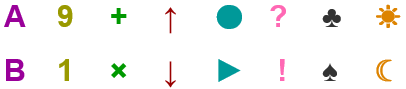
\includegraphics[scale=2]{../figuras/brm/Features8.png}
	\caption{
	% Pictured above are the features, the visual representation of the positive and negative values of the propositional variables. The upper row represents positive values of the propositional variables, while the lower row represents their negation.
	En la imagen de arriba se muestran las características, la representación visual de los valores positivos y negativos de las variables proposicionales. La fila superior representa valores positivos de las variables proposicionales, mientras que la fila inferior representa su negación.}
	\label{Figure:references}
\end{center}
\end{figure}


% \paragraph{Elements (boxes)\textemdash valuations.} A valuation over the propositional variables is visually represented as a square/box with the values (icons) of all propositional variables set at random positions inside the square. We call such representation an `element' (see Figure~\ref{Figure:element} for an example of such an element). The reason for choosing this representation is to avoid directional biases that could influence learning, and to exclude ordering and other operators from the language of thought (see \S\ref{Experiment_design} for more details). 
% Each time an element is shown (in particular, within the loop in the training-feedback) a new random position is chosen for the propositional features inside it.
\paragraph{Elementos (cajas) -- valuaciones.} Una valuación sobre las variables proposicionales se representa visualmente como un cuadrado/caja con los valores (íconos) de todas las variables proposicionales colocadas en posiciones aleatorias dentro de la caja. Llamamos a esta representación un `elemento' (ver Figura~\ref{Figure:element} para ver un ejemplo de tal elemento). La razón para elegir esta representación es evitar sesgos direccionales que podrían influir en el aprendizaje y excluir el orden y otros operadores del lenguaje del pensamiento (consultar \S\ref{Experiment_design} para obtener más detalles).
Cada vez que se muestra un elemento (en particular, dentro del ciclo en la etapa de entrenamiento-{\em feedback}) se elige una nueva posición aleatoria para las características proposicionales dentro de él.


\begin{figure}[h!] 
\begin{center}
    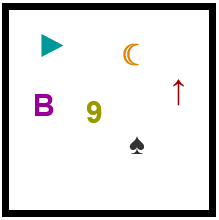
\includegraphics[scale=0.6]{../figuras/brm/BordeNeutro.PNG}
	\caption{
	% An element. This box containing features is the visual representation of a valuation over six propositional variables. Here the box appears with a neutral border, but boxes in the experiment always appear with a border that denotes whether they are positive or negative examples. The position of the symbols is irrelevant for the concepts, and is randomly assigned.
	Un elemento. Esta caja que contiene características es la representación visual de una valuación sobre seis variables proposicionales. Aquí la caja aparece con un borde neutro, pero las cajas del experimento siempre aparecen con un borde que denota si son ejemplos positivos o negativos. La posición de los símbolos es irrelevante para los conceptos y se asigna al azar.}
	\label{Figure:element} 
\end{center}
\end{figure}


% \paragraph{Undetermined concepts\textemdash sets of positive/negative valuations.}\label{IncompleteConcepts} The concept shown in the learning stage of a trial corresponds to two non-overlapping sets of valuations, and these two sets do not cover all possible valuations. This is represented as a sequence of `in' and `out' elements, with no information given on elements that are not shown.  At the learning stage, shown `in' elements (positive examples) are represented as a green box and shown `out' elements (negative examples) as a red box. See Figure~\ref{Figure:training} for an example of a tagged sequence of elements used in the learning stage. Each time the concept is presented, we shuffle the order in which their positive and negative examples are shown, but always presenting all positive examples first (also, each valuation is assigned new random positions for the features inside the corresponding box). 
\paragraph{Conceptos indeterminados -- conjuntos de valuaciones positivas/negativas.} \label{IncompleteConcepts} El concepto que se muestra en la etapa de aprendizaje de una prueba corresponde a dos conjuntos de valuaciones que no se superponen, y estos dos conjuntos no cubren todas las valuaciones posibles. Esto se representa como una secuencia de elementos `dentro' y `fuera', sin información sobre los elementos que no se muestran. En la etapa de aprendizaje, los elementos `dentro' (ejemplos positivos) se representan como una caja con borde verde y los elementos `fuera' (ejemplos negativos) como una caja con borde rojo. Consultar la Figura~\ref{Figure:training} para ver un ejemplo de una secuencia etiquetada de elementos utilizados en la etapa de aprendizaje. Cada vez que se presenta el concepto, barajamos el orden en el que se muestran sus ejemplos positivos y negativos, pero siempre presentando todos los ejemplos positivos primero (además, a cada valuación se le asignan nuevas posiciones aleatorias para las características dentro de la caja correspondiente).

\begin{figure}[h!] 
\begin{center}
    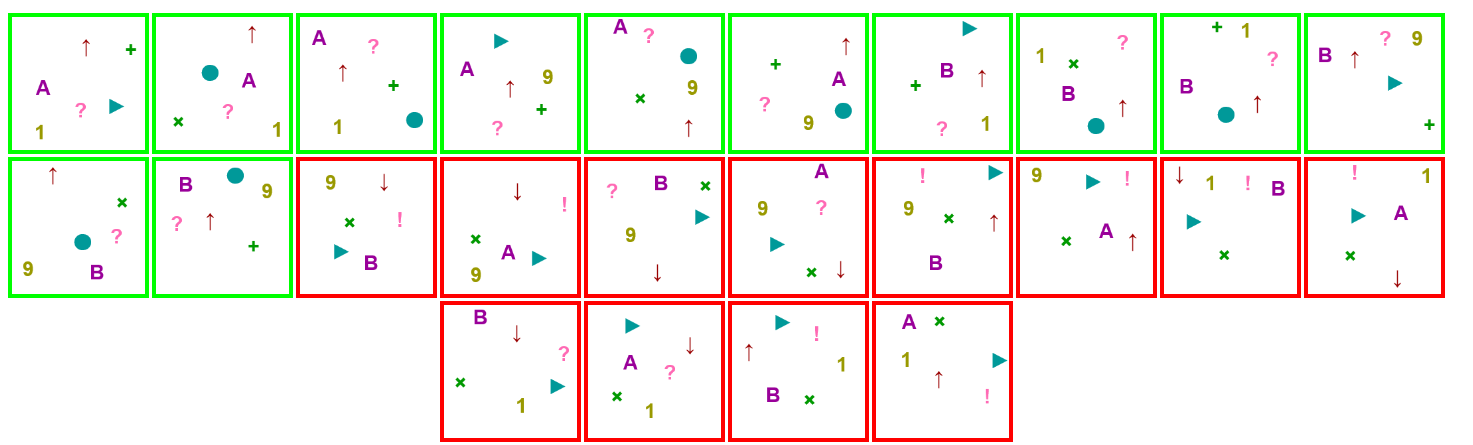
\includegraphics[scale=0.35]{../figuras/brm/Learning.PNG}
	\caption{
	% A sequence of positive and negative examples in a learning stage, corresponding to Trial 1.  A green border informs the participant that the element belongs to the concept, while a red-bordered one informs that it does not belong to the concept. In this case, the examples could be explained as either `boxes containing both an upwards pointing arrow and a question mark' or as `boxes that contain a circle or a plus sign', but note that these two rules determine different concepts over the complete set of possible elements.
	Una secuencia de ejemplos positivos y negativos en una etapa de aprendizaje, correspondiente a la Prueba 1. Un borde verde informa al participante que el elemento pertenece al concepto, mientras que un borde rojo informa que no pertenece al concepto. En este caso, los ejemplos podrían explicarse como `cajas que contienen una flecha que apunta hacia arriba y un signo de interrogación' o como `cajas que contienen un círculo o un signo más', pero hay que tener en cuenta que estas dos reglas determinan conceptos diferentes sobre el conjunto completo de posibles elementos.}
	\label{Figure:training}
\end{center}
\end{figure}

% \paragraph{(Hidden) concepts\textemdash formulas.}
% Over the full set of valuations, a concept is simply the set of valuations that positively describe it. The two hidden concepts for each trial correspond to the valid and minimal generalizations that can be made from the incomplete concepts. They can be described as the semantics of the two propositional formulas (rules) that can be used to explain the incomplete concept (see Table~\ref{trial_table}); while these rules coincide over the incomplete universe shown in the learning stage, they differ over the set of all valuations. For more details, recall the beginning of \S\ref{Subsec:ExperimentFlow} and its Item~\ref{item:LearningStage}. For technical details, see \S\ref{Sec:MainTheoremConcept}.
\paragraph{Conceptos (ocultos) -- fórmulas.}
Sobre el conjunto completo de valuaciones, un concepto es simplemente el conjunto de valuaciones que lo describen positivamente. Los dos conceptos ocultos para cada prueba corresponden a las generalizaciones válidas y mínimas que se pueden hacer a partir de los conceptos incompletos. Pueden describirse como la semántica de las dos fórmulas proposicionales (reglas) que pueden usarse para explicar el concepto incompleto (ver Tabla~\ref{trial_table}); si bien estas reglas coinciden en el universo incompleto que se muestra en la etapa de aprendizaje, difieren en el conjunto de todas las valuaciones. Para obtener más detalles, recordar el comienzo de \S\ref{Subsec:ExperimentFlow} y su ítem~\ref{item:LearningStage}. Para obtener detalles técnicos, consultar \S\ref{Sec:MainTheoremConcept}.

\bigskip

% In Table~\ref{tab:glosario} we summarize the main logical terminology used to define formal semantics, and its representational counterpart adopted in our experimental setup.



% \subsection{Details of the experiment's structure} \label{FullExperimentDescription} 
\subsection{Detalles de la estructura del experimento} \label{FullExperimentDescription} 

% As we explain in Section~\ref{Section:Experiment}, each instance of the experiment consists of 6 trials where the participants must learn a concept from an incomplete universe. The presented positive and negative examples are such that there are exactly two minimal rules (up to logical equivalence) in propositional logic that {\em 1)} are consistent explanations for the shown examples; {\em 2)} use disjoint sets of variables from each another; and {\em 3)} any rule consistent with the examples must use a superset of the set of features of at least one of these minimal rules. This experimental setup will allow us to distinguish which of these rules best represents the way that the participant learned the concept. See \S\ref{Sec:MainTheoremConcept} for technical details.
Como explicamos en la Sección~\ref{Section:Experiment}, cada instancia del experimento consta de~6 pruebas en las que los participantes deben aprender un concepto de un universo incompleto. Los ejemplos positivos y negativos presentados son tales que hay exactamente dos reglas mínimas (salvo equivalencia lógica) en la lógica proposicional que {\em 1)} son explicaciones consistentes para los ejemplos mostrados; {\em 2)} usan conjuntos de variables disjuntos entre sí; y {\em 3)} cualquier regla consistente con los ejemplos debe usar un superconjunto del conjunto de características de al menos una de estas reglas mínimas. Esta configuración experimental nos permitirá distinguir cuál de estas reglas representa mejor la forma en que el participante aprendió el concepto. Consultar \S\ref{Sec:MainTheoremConcept} para los detalles técnicos.


% Observe that merely asking the participant to select already seen elements does not give us any obvious insight into the internal process that derived into the learning of the concept; even if they internalized the concept using one of the two rules, it would remain uncertain which one they used, as both rules have the same semantics over the shown universe. In order to distinguish between these two cases, we use a generalization stage where previously unseen elements of the universe are shown, and the participant must select those that they believe belong to the concept. Of these new elements, some are consistent with only one of the rules, and other are consistent only with the other rule\footnote{The Trial 6 is an exception, and has an element that is consistent with both rules.}. Furthermore, immediately afterwards we ask for a written explanation of what characteristics the participant thinks describe the  concept.
Observar que el simple hecho de pedirle al participante que seleccione elementos ya vistos no nos da una idea obvia del proceso interno que derivó en el aprendizaje del concepto; incluso si internalizaran el concepto usando una de las dos reglas, sería incierto cuál usaron, ya que ambas reglas tienen la misma semántica sobre el universo mostrado. Para distinguir entre estos dos casos, utilizamos una etapa de generalización donde se muestran elementos del universo {\em nunca antes vistos}, y el participante debe seleccionar aquellos que crea que pertenecen al concepto aprendido. De estos nuevos elementos, algunos son consistentes con solo una de las reglas, y otros son consistentes solo con la otra regla\footnote{La Prueba 6 es una excepción y tiene un elemento que es consistente con ambas reglas.}. Además, inmediatamente después pedimos una explicación por escrito de las características que el participante cree que describen el concepto.

% Structurally, the experiment begins with the (hidden) assignment of the participant to one of two groups X or Y (see Table~\ref{trial_table}) and the exposition to a page with instructions. 
% Afterwards, there are 6 trials with the following structure: they begin with a learning stage; they continue to a training stage where they get feedback if they fail to correctly select the elements that belong to the concept; a generalization stage where they must choose between elements of the universe that were not shown previously; and, in all but the last trial, a stage where the participants can rest between trials.
Estructuralmente, el experimento comienza con la asignación (oculta) del participante a uno de los dos grupos X o Y (ver Tabla~\ref{trial_table}) y la exposición a una página con instrucciones.
Posteriormente, se realizan 6 pruebas con la siguiente estructura: comienzan con una etapa de aprendizaje; continúan a una etapa de entrenamiento donde reciben {\em feedback} si no seleccionan correctamente los elementos que pertenecen al concepto; una etapa de generalización donde deben elegir entre elementos del universo que no fueron mostrados previamente; y, en todos menos en la última prueba, una etapa en la que los participantes pueden descansar entre ensayos.

% In what follows, we describe each stage of the experiment plus the introductory page, with a greater detail than that of \S\ref{Subsec:ExperimentFlow}.
A continuación, describimos cada etapa del experimento más la página de introducción, con mayor detalle que en \S\ref{Subsec:ExperimentFlow}.

% \subsubsection{Introduction and explanation}
\subsubsection{Introducción y explicación}

% This is the page that subjects are shown at the beginning of the experiment. It describes the main task they will be asked to perform: that of learning from examples to distinguish what kind of `boxes' belong to a certain concept. These elements are represented as a collection of 6 symbols, no more than one from a same pair. It is also informed that the position of the symbols does not matter. See Figure~\ref{Figure:element} for an example element.
Esta es la página que se muestra a los sujetos al comienzo del experimento. Describe la tarea principal que se les pedirá que realicen: la de aprender de ejemplos para distinguir qué tipo de `cajas' pertenecen a un determinado concepto. Estos elementos se representan como una colección de 6 símbolos, no más de uno de un mismo par. También se le informa que la posición de los símbolos no importa. Consultar la Figura~\ref{Figure:element} para ver un elemento de ejemplo.

% When the subject indicates they have finished reading the instructions, they are sent to a fullscreen page with three multiple-choice questions whose purpose is to verify that the participant has understood the instructions; if they miss some answer, they are returned to the previous page and the cycle is repeated until they succeed.
Cuando el sujeto indica que ha terminado de leer las instrucciones, se lo envía a una página de pantalla completa con tres preguntas de opción múltiple cuyo propósito es verificar que el participante ha entendido las instrucciones; si se equivoca en alguna respuesta, vuelve a la página anterior y el ciclo se repite hasta que lo consigue.

% If the participant answers correctly, they are now ready to begin, and the phases~\S\ref{Subsection:learning}, \S\ref{Subsection:training}, and \S\ref{Subsection:generalization} are then entered sequentially for each of the 6 trials.
Si el participante responde correctamente, está listo para comenzar, y se ingresan a las fases~\S\ref{Subsection:learning}, \S\ref{Subsection:training}, y \S\ref{Subsection:generalization} secuencialmente para cada uno de los 6 ensayos.

% \subsubsection{The learning phase}\label{Subsection:learning}
\subsubsection{La fase de aprendizaje}\label{Subsection:learning}

% In this phase of a Trial $i$, the participant is shown a set $S^i \subsetneq U^i$, a proper subset of elements from the current universe. Each universe syntactically corresponds to all the combinations of truth values for 6 propositional variables taken from the set $\{\varA, \varB, \varC, \varD, \varE, \varF, \varG, \varH\}$, thus spawning a set $U^i$ of 64 elements. On the semantic side we call `features' the visual representations of the propositional variables, and these representations remain fixed through the experiment (recall Figure~\ref{Figure:references}).
En esta fase de una prueba $ i $, al participante se le muestra un $ S^i \subsetneq U^i $, un subconjunto adecuado de elementos del universo actual. Cada universo corresponde sintácticamente a todas las combinaciones de valores de verdad para 6 variables proposicionales tomadas del conjunto $\{\varA, \varB, \varC, \varD, \varE, \varF, \varG, \varH\}$, por lo tanto generando un conjunto $ U^i $ de 64 elementos. Del lado semántico, llamamos `características' a las representaciones visuales de las variables proposicionales, y estas representaciones permanecen fijas durante el experimento (recordar la Figura~\ref{Figure:references}).

% The elements of $S^i$ are shown as boxes, some of which have green border (denoting a positive example, that the element belongs to the concept), while the rest have red borders (denoting a negative example, that they do not belong).The green-bordered boxes are shown first, with the red-bordered ones appearing after the last box with green border. See Figure~\ref{Figure:training} for an example learning set. 
Los elementos de $ S^i $ se muestran como cajas, algunas de las cuales tienen borde verde (que denota un ejemplo positivo, es decir que el elemento pertenece al concepto), mientras que el resto tiene bordes rojos (que denota un ejemplo negativo, es decir que no lo hacen). Las cajas de borde verde se muestran primero, y las de borde rojo aparecen después de la última caja con borde verde. Consultar la Figura~\ref{Figure:training} para ver un ejemplo de conjunto de aprendizaje.

% If the graphical representations are abstracted away to the underlying basic structure, there are two propositional rules $\varphi^i_1$ and $\varphi^i_2$ (of minimum length in their class of logically equivalent rules, see Table~\ref{trial_table}) whose semantics correctly classify the positive and negative examples shown. If we call $C^i_1, C^i_2$ the sets of valuations that satisfy $\varphi^i_1, \varphi^i_2$, respectively, we have that $S^i = (C^i_1 \cap C^i_2) \cup \overline{(C^i_1 \cup C^i_2)}$. The rules $\varphi^i_1, \varphi^i_2$ use at most\footnote{The rules that are actually `learnable' use exactly 2 propositional variables.} 3 of the 6 propositional variables available in $U^i$, and the two rules do not have propositional variables in common. 
Si las representaciones gráficas se abstraen de la estructura básica subyacente, hay dos reglas proposicionales $ \varphi^i_1 $ y $ \varphi^i_2 $ (de longitud mínima en su clase de reglas lógicamente equivalentes, consultar la Tabla~\ref{trial_table}) cuya semántica clasifica correctamente los ejemplos positivos y negativos mostrados. Si llamamos $ C^i_1, C^i_2 $ a los conjuntos de valuaciones que satisfacen $ \varphi^i_1, \varphi^i_2 $, respectivamente, tenemos que $ S^i = (C^i_1 \cap C^i_2) \cup \overline {(C^i_1 \cup C^i_2)} $. Las reglas $ \varphi^i_1, \varphi^i_2 $ usan a lo sumo\footnote{Las reglas que son realmente `aprendibles' usan exactamente 2 variables proposicionales.} 3 de las 6 variables proposicionales disponibles en $ U^i $, y las dos reglas no tienen variables proposicionales en común.

% When the participant believes they have learned which elements belong to the concept, they can click a button to proceed to the next stage.
Cuando el participante cree que ha aprendido qué elementos pertenecen al concepto, puede hacer clic en un botón para pasar a la siguiente etapa.

% \subsubsection{The training\textendash feedback phase}\label{Subsection:training}
\subsubsection{La fase de entrenamiento\textendash{\em feedback}}\label{Subsection:training}

% In this phase, the participant is shown a random rearrangement of $S^i$, with all the elements now surrounded by a red-bordered square. The subject must click exactly those elements (if any) they believe belong to the concept \textemdash changing them to a dotted green border (see Figure~\ref{Figure:ElementSquares})\textemdash\ and then has to click a button to submit their choice.
En esta fase, al participante se le muestra un reordenamiento aleatorio de $S^i $, con todos los elementos ahora rodeados por un cuadrado con borde rojo. El sujeto debe hacer clic exactamente en aquellos elementos (si los hay) que cree que pertenecen al concepto --cambiándolos a un borde verde punteado (ver Figura~\ref{Figure:ElementSquares})-- y luego debe hacer clic en un botón para enviar su elección.

\begin{figure}[h!] 
\begin{center}
    	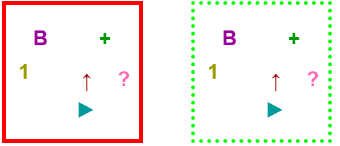
\includegraphics[scale=0.6]{../figuras/brm/SelectionSeparadosIguales.png}
	\caption{
	% An unselected element, to the left, is represented by solid red borders. The same element in a selected state, to the right, is indicated by dotted green borders.
	Un elemento no seleccionado, a la izquierda, está representado por bordes rojos sólidos. El mismo elemento en un estado seleccionado, a la derecha, se indica con bordes verdes punteados.}
	\label{Figure:ElementSquares}
\end{center}
\end{figure}

% If their selection  is  incorrect, the participant is shown which elements they misclassified (either by clicking them incorrectly or by failing to click them, see Figure~\ref{Figure:Misclassifications}). When they click a button to continue, they restart this stage (with a fresh randomization).
Si su selección es incorrecta, se le muestra al participante qué elementos clasificaron erróneamente (ya sea haciendo clic en ellos incorrectamente o no haciendo clic en ellos, consulte la Figura~\ref{Figure:Misclassifications}). Cuando hacen clic en un botón para continuar, reinician esta etapa (con una nueva mezcla aleatoria en la posición de las cajas y los símbolos dentro de ellas).

\begin{figure}[h!] 
\begin{center}
    	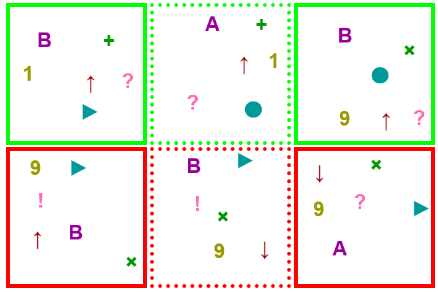
\includegraphics[scale=0.5]{../figuras/brm/FeedBack2SeleccionParcial.PNG}
	\caption{
	% A partial section of the feedback resulting from a wrong selection. A solid green border means that the box was correctly selected as belonging to the concept. A solid red border means that it was correctly left unselected, meaning that it did not belong to the concept. A dotted green border means the box belongs to the concept but was not selected, and a dotted red border means that the box does not belong to the concept but was selected.
	Una sección parcial del {\em feedback} resultante de una selección incorrecta. Un borde verde sólido significa que la casilla se seleccionó correctamente como perteneciente al concepto. Un borde rojo sólido significa que se dejó sin seleccionar correctamente, lo que significa que no pertenecía al concepto. Un borde verde punteado significa que la caja pertenecía al concepto pero no fue seleccionado, y un borde rojo punteado significa que la caja no pertenecía al concepto pero fue seleccionado.}
	\label{Figure:Misclassifications}
\end{center}
\end{figure}

% When the participant finally makes the correct selection, they continue to the next phase. 
Cuando el participante finalmente hace la selección correcta, pasa a la siguiente fase.

% \subsubsection{The generalization phase}\label{Subsection:generalization}
\subsubsection{La fase de generalización}\label{Subsection:generalization}

% In this phase, the participant is shown a subset of $U^i \backslash S^i$ (namely, in $(C^i_1 \cup C^i_2) \backslash (C^i_1 \cap C^i_2)$), that is, a selection of elements that were \emph{not} present in the learning phase (hence nor in the training phase). The participant must classify which of these elements they think belong to the concept. The participant does not receive feedback on the choices they make here. Except for the sixth trial, part of these elements satisfy the rule $\varphi^i_1 \land \lnot \varphi^i_2$, while the rest satisfy $\varphi^i_2 \land \lnot \varphi^i_1$. Thus \textemdash assuming the participant learned the concept via a process akin to a representation of one of the two rules\textemdash\, this phase crucially serves to distinguish which rule they have learned, if any.
En esta fase, se muestra al participante un subconjunto de $U^i \backslash S^i $ (o sea, $(C^i_1 \cup C^i_2) \backslash (C^i_1 \cap C^i_2) $), es decir, una selección de elementos que \emph {no} estaban presentes en la fase de aprendizaje (por tanto, tampoco en la de aprendizaje). El participante debe clasificar cuáles de estos elementos cree que pertenecen al concepto. El participante no recibe comentarios sobre las elecciones que hace aquí. Excepto por la sexta prueba, parte de estos elementos satisfacen la regla $\varphi^i_1 \land \lnot \varphi^i_2$, mientras que el resto satisface $\varphi^i_2 \land \lnot \varphi^i_1$. Por lo tanto, --asumiendo que el participante aprendió el concepto a través de un proceso similar a la representación de una de las dos reglas--, esta fase sirve de manera crucial para distinguir qué regla ha aprendido, si es que ha aprendido alguna.

% After this selection, the participant is asked to submit a written explanation of what characteristics they think constitute the concept. This written explanation serves as an additional validation of whether they are thinking in a way describable by propositional logic according to our assumptions, or if rather they are using other methods (memorization, pen and paper, screenshots, other logics or formalisms, etc.). 
Después de esta selección, se solicita al participante que presente una explicación por escrito de lo que cree que define al concepto. Esta explicación escrita sirve como una validación adicional de si están pensando de una manera descriptible por lógica proposicional según nuestros supuestos, o si más bien están usando otros métodos (memorización, lápiz y papel, capturas de pantalla, otras lógicas o formalismos, etc.).

% \subsection{Notes on the experiment design}\label{Experiment_design}
\subsection{Notas sobre el diseño del experimento}\label{Experiment_design}


% The elements, universes, and rules that constitute our experiment are devised in terms of propositional logic. However, it is important to be careful with the semantics, i.e.\ the way elements are actually shown to the participants. We have to avoid giving more salience to the semantics of a propositional variable over the others, and it is imperative to select the semantics of variables in a way such that they do not share characteristics that might escape our propositional grammar: for example, if the propositional variables were represented as circles that can be distinctly colored or not, it would be quite natural to assume that counting colored or uncolored circles could provide information, but this option is not considered in a theoretical design that assumes only propositional operators to describe rules. A related consideration is that we must also avoid introducing other regularities extraneous to the propositional formulation: if the images corresponding to all propositional variables are always shown in a straight line in the same order, salience effects might appear \textit{even if }we avoid semantics that become more expressive thanks to the ordered nature of the represented variables (such as with descriptions of the form \textit{the first and last elements are of the same size}).
Los elementos, universos y reglas que constituyen nuestro experimento están diseñados en términos de lógica proposicional. Sin embargo, es importante ser cuidadosos con la representación de la semántica, es decir, la forma en que los elementos se muestran realmente a los participantes. Tenemos que evitar dar más prominencia a la semántica de una variable proposicional sobre las demás, y es imperativo seleccionar la semántica de las variables de tal manera que no compartan características que puedan escapar a nuestra gramática proposicional: por ejemplo, si las variables proposicionales se representaron como círculos que pueden tener distintos colores o no (como fue el caso del experimento del Capítulo~\ref{chapter:PRE}), sería bastante natural suponer que contar círculos coloreados o no coloreados podría proporcionar información. Sin embargo, esta opción no se considera en un diseño teórico que asume solo operadores proposicionales para describir reglas. Una consideración relacionada es que también debemos evitar introducir otras regularidades ajenas a la formulación proposicional: si las imágenes correspondientes a todas las variables proposicionales se muestran siempre en línea recta en el mismo orden, los efectos de prominencia pueden aparecer \textit{incluso si} evitamos semánticas que se vuelven más expresivas gracias a la naturaleza ordenada de las variables representadas (como con descripciones de la forma \textit{el primer y último elemento son del mismo tamaño}).


% \paragraph{Building adequate semantic representations for our logic.}
\paragraph{Construyendo representaciones semánticas adecuadas para nuestra lógica.}

% Taking these precautions into account, we choose to match each propositional variable with a particular image or figure, whose position in a square would be randomized (but avoiding superpositions). It  is harder to decide exactly what would be the matching, but our final decision consists in matching each propositional variable with a set of two related Unicode characters (such as a triangle when the variable is $0$, and a circle otherwise). See Figure~\ref{Figure:references} for the exact representations. We take care to choose different types of characters for different variables: having $A,B$ for $\varA$ and $Y,Z$ for $\varE$ is out as a possibility, since it naturally  introduces counting of the type `there is no more than 1 letter' and the like. Of course, this process is not fail-safe, as there are countless possible semantics associations that could introduce extra-propositional grammar into the experiment. But we try to minimize the chance that this happens easily or naturally, and we use the written explanation stage as a way to catch these exceptions if they occur\footnote{In the end, they did not occur. See \S\ref{Sec:ExclusionCriteria}.}. 
Teniendo en cuenta estas precauciones, decidimos mejorar la representación respecto a la usada en el Capítulo~\ref{chapter:PRE} y optamos por hacer coincidir cada variable proposicional con una imagen o figura en particular, cuya posición en un cuadrado sería aleatoria (pero evitando superposiciones). Es difícil decidir exactamente cuál sería la mejor coincidencia de variable a imagen, pero nuestra decisión final consiste en hacer coincidir cada variable proposicional con un conjunto de dos caracteres Unicode relacionados (como un triángulo cuando la variable es $ 0 $ y un círculo en caso contrario). Ver la Figura~\ref{Figure:references} para las representaciones exactas. Nos encargamos de elegir diferentes tipos de caracteres para diferentes variables: tener $ A, B $ para $ \varA $ y $ Y, Z $ para $ \varE $ no es una posibilidad, ya que naturalmente introduce el conteo del tipo `no hay más de 1 letra' y similares. Por supuesto, este proceso no es completamente seguro, ya que existen innumerables asociaciones semánticas posibles que podrían introducir gramáticas extra-proposicionales en el experimento. No obstante, tratamos de minimizar la posibilidad de que esto suceda fácil o naturalmente, y usamos la etapa de explicación escrita como una forma de detectar estas excepciones, si ocurriesen\footnote {Al final, no ocurrieron. Consultar \S\ref{Sec:ExclusionCriteria}.}.

% Finally, to minimize possible salience effects from showing symbols that could have (despite our intentions to the contrary) different levels of conspicuousness, we randomize on a per-participant basis the assignment between pairs of symbols and propositional variables (but we do not randomize  the assignment to the positive or negative value of a variable; the same Unicode characters  are  always positive in all randomizations, or always negative).
Finalmente, para minimizar los posibles efectos de prominencia de mostrar símbolos que podrían tener (a pesar de nuestras intenciones en la dirección contraria) diferentes niveles de notoriedad, aleatorizamos por participante la asignación entre pares de símbolos y variables proposicionales (pero no aleatorizamos la asignación al valor positivo o negativo de una variable; los mismos caracteres Unicode son siempre positivos en todas las aleatorizaciones, o siempre negativos).

% \paragraph{Ordering of positive and negative examples.}
\paragraph{Orden de ejemplos positivos y negativos.}

% As mentioned before, in the learning stage we shuffle the order in which their positive and negative examples are shown, but always presenting all positive examples first. Also, the number of positive examples is smaller or equal to the number of negative examples for all concepts (see Table \ref{trial_table}). 
Como se mencionó anteriormente, en la etapa de aprendizaje cambiamos el orden en el que se muestran los ejemplos positivos y negativos, pero siempre presentando todos los ejemplos positivos primero. Además, el número de ejemplos positivos es menor o igual al número de ejemplos negativos para todos los conceptos (ver Tabla~\ref{trial_table}).

% The purpose of placing the positive examples first and having less positive examples than negative ones is to bias the participant into thinking of the concept by its positive formulation, instead of possibly thinking of a rule that would describe the negative examples, and then negating that rule to obtain the positive one. This becomes important when we want to reason about the ease of learning of different operators: the default assumption is that participants that correctly select positive examples of the concept are thinking the positive rule, which differs in its operator from the negative rule (by the De Morgan laws). 
El propósito de colocar los ejemplos positivos al principio y tener menos ejemplos positivos que negativos es sesgar al participante para que piense en el concepto por su formulación {\em positiva}, en lugar de pensar posiblemente en una regla que describa los ejemplos negativos, y luego negar esa regla para obtener el positivo. Esto se vuelve importante cuando queremos razonar sobre la facilidad de aprendizaje de diferentes operadores: la suposición predeterminada es que los participantes que seleccionan correctamente ejemplos positivos del concepto están pensando en la regla positiva, que difiere en su operador de la regla negativa (por las leyes de De Morgan).


% \section{Results}\label{Results}
\section{Resultados}\label{Results}


% \subsection{Hypothesis~\ref{Hip:AndOverOr}}\label{Results:AndOverOr}
\subsection{Hipótesis~\ref{Hip:AndOverOr}}\label{Results:AndOverOr}

% We asked whether the conjunction-disjunction bias (which is known to affect learning times in the case of a single explanation~\cite{bourne1970knowing}) also determines which features are used to describe a concept when two alternative explanations are consistent with the observed universe. In the first trial, the observed examples were consistent with $p_1 \vee p_2$ and with $p_3 \wedge p_4$. As explained in \S\ref{Subsec:ExperimentFlow}, in the generalization stage we can determine if participants explained the concept using $\{p_1,p_2\}$ or $\{p_3,p_4\}$. We found that 77 of the 100 participants attended to $\{p_3,p_4\}$, which corresponds to an explanation that uses a conjunction. 11 participants attended to $\{p_1,p_2\}$ (corresponding to the use of a disjunction for the explanation), and 12 participants selected examples in the generalization stage inconsistent with both $p_3 \wedge p_4$ and $p_1 \vee p_2$. To test the significance of this result, we performed a permutation test. Under the null hypothesis that participants randomly choose between explaining the concept using features $\{p_1,p_2\}$ and explaining it using $\{p_3,p_4\}$, the probability that 77 of the 100 participants attend to $\{p_3,p_4\}$ is $P<10^{-12}$. Thus we conclude that the observed difference is significant. 
Nos preguntamos si el sesgo de conjunción-disyunción (que se sabe que afecta los tiempos de aprendizaje en el caso de una explicación única~\cite{bourne1970knowing}) también determina qué características se usan para describir un concepto cuando dos explicaciones alternativas son consistentes con el universo observado. En la primera prueba, los ejemplos observados fueron consistentes con $ p_1 \vee p_2 $ y con $ p_3 \wedge p_4 $. Como se explica en \S\ref{Subsec:ExperimentFlow}, en la etapa de generalización podemos determinar si los participantes explicaron el concepto usando $ \{p_1, p_2 \} $ o $ \{p_3, p_4 \} $. Encontramos que 77 de los 100 participantes prestaron atención a $ \{p_3, p_4 \} $, que corresponde a una explicación que usa una conjunción. 11 participantes se enfocaron a $ \{p_1, p_2 \} $ (correspondiente al uso de una disyunción para la explicación), y 12 participantes seleccionaron ejemplos en la etapa de generalización inconsistentes con $ p_3 \wedge p_4 $ y $ p_1 \vee p_2$. Para probar la importancia de este resultado, realizamos una prueba de permutación. Bajo la hipótesis nula de que los participantes eligen aleatoriamente entre explicar el concepto usando las características $ \{p_1, p_2 \} $ y explicarlo usando $ \{p_3, p_4 \} $, la probabilidad de que 77 de los 100 participantes asistan a $ \{ p_3, p_4 \} $ es $ p <10^{-12} $. Por tanto, concluimos que la diferencia observada es significativa.

% Note that it is in principle possible that the participant learned the concept with a focus on negative examples ({\sf B}'s in Figure~\ref{fig:trials}) instead of on positive examples ({\sf A}'s in Figure~\ref{fig:trials}) (i.e. finding a correct explanation for the negative examples and then negating that rule to obtain an explanation for the positive examples). 
Hay que tener en cuenta que, en principio, es posible que el participante haya aprendido el concepto con un enfoque en ejemplos negativos ({\sf B}s en la Figura~\ref{fig:trials}) en lugar de en ejemplos positivos ({\sf A}s en la Figura~\ref{fig:trials}) (es decir, encontrar una explicación correcta para los ejemplos negativos y luego negar esa regla para obtener una explicación para los ejemplos positivos).

% As we mention in \S\ref{Experiment_design}, we induced a bias to understand the concept in the appropriate way by first presenting the positive examples in the learning phase and by asking them to click on the positive ones in the training phase. We note, however, that 9 participants gave verbal explanations consistent with focusing on the negative examples. In this particular trial, a reverse interpretation is problematic since the negation of a conjunction corresponds to a disjunction, and the negation of the disjunction to a conjunction (i.e.\ $p\land q$ is logically equivalent to $\lnot(\lnot p\lor \lnot q)$). Thus, a more comprehensive analysis should take into account participants' verbal explanations in this trial. However, even considering the worst-case scenario in which these 9 participants were originally regarded as part of the `conjunction' group and they are now considered part of the `disjunction' group, the conjunction-disjunction bias is still significant ($P<10^{-7}$). We therefore conclude that, in this framework where multiple explanations are possible depending on the attended features, there is a bias favoring conjunctive explanations over disjunctive explanations. 
Como mencionamos en \S\ref{Experiment_design}, indujimos un sesgo para comprender el concepto de la manera adecuada, presentando primero los ejemplos positivos en la fase de aprendizaje y pidiéndoles que hicieran clic en los positivos en la fase de entrenamiento. Sin embargo, observamos que nueve participantes dieron explicaciones verbales coherentes con el enfoque en los ejemplos negativos. En esta prueba en particular, una interpretación inversa es problemática ya que la negación de una conjunción corresponde a una disyunción, y la negación de la disyunción a una conjunción (es decir, $ p \land q $ es lógicamente equivalente a $ \lnot (\lnot p \lor \lnot q) $). Por lo tanto, un análisis más completo debe tener en cuenta las explicaciones verbales de los participantes en esta prueba. Sin embargo, incluso considerando el peor escenario en el que estos 9 participantes fueran considerados originalmente como parte del grupo de  `conjunción' y ahora se consideren parte del grupo de `disyunción', el sesgo de conjunción-disyunción sigue siendo significativo ($ p<10^{-7} $). Por lo tanto, concluimos que, en este marco donde son posibles múltiples explicaciones dependiendo de las características enfocadas, existe un sesgo que favorece las explicaciones conjuntivas sobre las explicaciones disyuntivas.

% \subsection{Hypothesis \ref{Hip:FeatureBiasStickiness}}\label{Results:FeatureBiasStickiness}
\subsection{Hipótesis \ref{Hip:FeatureBiasStickiness}}\label{Results:FeatureBiasStickiness}

% Most participants understood the concept in Trial 6 using the same features $\{p_7,p_8\}$ used to describe the concept in Trial~5, even when the logical structure of the rule was exactly the same independently of attending to $\{p_7,p_8\}$ or to $\{p_3,p_4\}$\footnote{As expected by our experiment design, 94 of the 100 participants understood the concept in Trial 5 using features $\{p_7,p_8\}$ (6 selected features with no clear rationale). Using features $\{p_7,p_8\}$ is indeed the only plausible way to learn the concept, given the high complexity of the alternative MDL15 formula. }. To show this, we study participants' choices in the generalization stage of Trial 6 (see Figure~\ref{fig:results1}). 
La mayoría de los participantes entendieron el concepto en la Prueba 6 usando las mismas características $ \{p_7, p_8 \} $ que se usaron para describir el concepto en la Prueba~5, incluso cuando la estructura lógica de la regla era exactamente la misma independientemente de prestar atención a $ \{ p_7, p_8 \} $ o $  \{p_3, p_4 \} $\footnote{Como se esperaba en el diseño de nuestro experimento, 94 de los 100 participantes entendieron el concepto en la Prueba 5 usando las características $ \{p_7, p_8 \} $ (6 características seleccionadas sin una justificación clara). Usar las características $ \{p_7, p_8 \} $ es de hecho la única forma plausible de aprender el concepto, dada la alta complejidad de la fórmula alternativa MDL15.}. Para mostrar esto, estudiamos las elecciones de los participantes en la etapa de generalización de la Prueba 6 (consultar la Figura~\ref{fig:results1}).

% Suppose that a participant is thinking of the rule $\lnot p_7 \land \lnot p_8$, thus they are only attending to features $\{p_7,p_8\}$ while ignoring the features $\{p_3,p_4\}$. Since $\{p_3,p_4\}$ are being ignored, the participant should mark those elements in which $\{p_7,p_8\}$ agrees with the rule $\lnot p_7 \land \lnot p_8$, irrespective of the values of $\{p_3,p_4\}$. That is, the participant should mark the elements with $\{p_3,p_4,p_7,p_8\}$ equal to $(0,0,\textbf{0,0})$, $(1,0,\textbf{0},\textbf{0})$, $(0,1,\textbf{0},\textbf{0})$ and $(1,1,\textbf{0},\textbf{0})$. These elements have $\{p_7,p_8\}$ equal to $(0,0)$ and `anything' for $\{p_3,p_4\}$. On the other hand, if the participant is thinking of the rule $p_3 \land \lnot p_7 \land \lnot p_8$, then she is attending to $\{p_3,p_7,p_8\}$, and she should mark $(\textbf{1},0,\textbf{0},\textbf{0})$ and $(\textbf{1},1,\textbf{0},\textbf{0})$. 
Supongamos que un participante en la Prueba 6 está pensando en la regla $ \lnot p_7 \land \lnot p_8 $, por lo que solo está dirigiendo su atención a las características $ \{p_7, p_8 \} $ mientras ignora las características $ \{p_3, p_4 \} $. Dado que se ignoran $ \{p_3, p_4 \} $, el participante debe marcar aquellos elementos en los que $ \{p_7, p_8 \} $ está de acuerdo con la regla $ \lnot p_7 \land \lnot p_8 $, independientemente de los valores de $ \{p_3, p_4 \} $. Es decir, el participante debe marcar los elementos con $ \{p_3, p_4, p_7, p_8 \} $ igual a $ (0,0, \textbf {0, 0}) $, $ (1,0, \textbf { 0}, \textbf {0}) $, $ (0,1, \textbf {0}, \textbf {0}) $ y $ (1,1, \textbf {0}, \textbf {0}) $. Estos elementos tienen $ \{p_7, p_8 \} $ igual a $ (0,0) $ y `cualquier valor' por $ \{p_3, p_4 \} $. Por otro lado, si el participante está pensando en la regla $ p_3 \land \lnot p_7 \land \lnot p_8 $, entonces está atendiendo a $ \{p_3, p_7, p_8 \} $, y debe marcar $ ( \textbf {1}, 0, \textbf {0}, \textbf {0}) $ y $ (\textbf {1}, 1, \textbf {0}, \textbf {0}) $.

% In general, by studying which of the 7 examples shown in Figure~\ref{fig:results1} (left) the participant selects in the generalization phase, we can deduce which features they were attending to (Figure~\ref{fig:results1}, right). For example, all participants should mark the example with $\{p_3,p_4,p_7,p_8\}$ equal to $(1,1,0,0)$, since it is consistent with all the logical rules irrespective of which features are used. 
En general, al estudiar cuál de los 7 ejemplos que se muestran en la Figura~\ref{fig:results1} (izquierda) selecciona el participante en la fase de generalización, podemos deducir qué características estaban atendiendo (Figura~\ref{fig:results1}, derecha). Por ejemplo, todos los participantes deben marcar el ejemplo con $ \{p_3, p_4, p_7, p_8 \} $ igual a $ (1,1,0,0) $, ya que es coherente con todas las reglas lógicas independientemente de las características son usadas.

% Indeed, as shown in Figure~\ref{fig:results1} (left), all participants selected this example. Although in practice the participant can select any of the 7 examples in the generalization stage, we found that all but five participants respected the rules of coherence illustrated in the previous paragraph. These 5 participants were `one example away' of respecting the rule, however, we leave them out of the feature stickiness analysis, but including them does not change our conclusions. We also excluded 6 participants that selected elements with no clear rationale in the previous trial, since they may not have used features $\{p_7,p_8\}$. However, including these participants (and assuming they did use $\{p_7,p_8\}$ in the previous trial) does not significantly change the results. In total, these two exclusions leaves 89 participants for this analysis. The grey lines in Figure~\ref{fig:results1} (left) show simulations of agents that randomly select one of the seven possible subsets of features, and then proceed to select the examples consistent with the logical rule using that features. Participants responses (black line) were biased towards explanations using $\{p_7,p_8\}$, as predicted by the feature-stickiness bias. This can also be seen in  Figure~\ref{fig:results1} (right), after inferring which features participants used to build the rule for the concept. In addition to being biased towards $\{p_7,p_8\}$, several participants explained the concept using all available features $\{p_3,p_4,p_7,p_8\}$. This shows that, in addition to the feature stickiness bias, when the number of features is relatively small, participants were also biased to describe the concept using all available features.
En efecto, como se muestra en la Figura~\ref{fig:results1} (izquierda), todos los participantes seleccionaron este ejemplo. Aunque en la práctica el participante puede seleccionar cualquiera de los 7 ejemplos en la etapa de generalización, encontramos que todos salvo cinco participantes respetaron las reglas de coherencia ilustradas en el párrafo anterior. Estos 5 participantes estuvieron `a un ejemplo de distancia' de respetar la regla, sin embargo, los dejamos fuera del análisis de adherencia de características, pero haberlos incluido no habría cambiado nuestras conclusiones. También excluimos a 6 participantes que seleccionaron elementos sin una justificación clara en la prueba anterior, ya que es posible que no hayan utilizado las características $ \{p_7, p_8 \} $. Sin embargo, la inclusión de estos participantes (y asumiendo que usaron $ \{p_7, p_8 \} $ en la prueba anterior) no cambia significativamente los resultados. En total, estas dos exclusiones dejan 89 participantes para este análisis. Las líneas grises en la Figura~\ref{fig:results1} (izquierda) muestran simulaciones de agentes que seleccionan aleatoriamente uno de los siete posibles subconjuntos de características, y luego proceden a seleccionar los ejemplos consistentes con la regla lógica usando esas características. Las respuestas de los participantes (línea negra) estuvieron sesgadas hacia las explicaciones usando $ \{p_7, p_8 \} $, como predijo el sesgo de adherencia de características. Esto también se puede ver en la Figura~\ref{fig:results1} (derecha), después de inferir qué características usaron los participantes para construir la regla para el concepto. Además de estar sesgados hacia $ \{p_7, p_8 \}$, varios participantes explicaron el concepto utilizando todas las características disponibles $ \{p_3, p_4, p_7, p_8 \} $. Esto muestra que, además del sesgo de adherencia de características, cuando el número de características es relativamente pequeño, los participantes también están predispuestos a describir el concepto utilizando todas las características disponibles.


% To quantify the feature stickiness bias, we assign a score to each participant according to the attended features in Trial 6 (deduced from the marked examples). The scores for the subsets $\{p_7,p_8\}$, $\{p_3,p_7,p_8\}$, $\{p_4,p_7,p_8\}$, $\{p_3,p_4,p_7,p_8\}$, $\{p_3,p_4,p_7\}$, $\{p_3,p_4,p_8\}$ and $\{p_3,p_4\}$ are 1, 2/3, 2/3, 1/2, 1/3, 1/3 and 0 respectively\footnote{Part (d) of the Analysis Plan section in our preregistration had a mistake in the use of features names: the learnable concept corresponding to the fifth trial uses $p_7$ and $p_8$, not $p_3$ and $p_4$ as erroneously written in that part; compare with the section on Study design, which matches Table~\ref{trial_table}.}. The average score for the 89 participants was 0.68 ($P<10^{-6}$ in a permutation test with the null hypothesis of randomly attending to one of the seven subsets of features, which correspond to the grey lines in Figure~\ref{fig:results1}), indicating a significant effect of the feature stickness bias. Although the feature stickiness bias was significant for both groups independently (Group X: average score 0.62, $P<10^{-5}$;  Group Y: average score 0.74, $P<10^{-6}$), we found that feature stickiness was higher in Group Y (two-sample t-test comparing the scores of the two groups shows $t=2.35$,  $P<0.05$). The only difference between the groups is that Group Y had already (artificially) experienced feature stickiness between the previous Trials 3 and 4, so they have already identified it as an useful bias for the task. This suggests that the entire concept-learning sequence can be important when studying learning biases. 
Para cuantificar el sesgo de adherencia de características, asignamos una puntuación a cada participante de acuerdo con las características atendidas en la Prueba 6 (deducida de los ejemplos marcados). Las puntuaciones de los subconjuntos $ \{p_7, p_8 \} $, $ \{p_3, p_7, p_8 \} $, $ \{p_4, p_7, p_8 \} $, $ \{p_3, p_4, p_7, p_8 \} $, $ \{p_3, p_4, p_7 \} $, $ \{p_3, p_4, p_8 \} $ y $ \{p_3, p_4 \} $ son 1, 2/3, 2/3, 1/2 , 1/3, 1/3 y 0 respectivamente\footnote{La parte (d) de la Plan de Análisis en nuestro pre-registro tenía un error en el uso de los nombres de las características: el concepto de aprendizaje correspondiente a la quinta prueba usa $ p_7 $ y $ p_8 $, no $ p_3 $ y $ p_4 $ como está escrito erróneamente en esa parte; comparar con la sección sobre diseño del estudio, que coincide con la Tabla~\ref{trial_table}.}. El puntaje promedio para los 89 participantes fue 0.68 ($ p <10^{- 6} $ en una prueba de permutación con la hipótesis nula de atender al azar a uno de los siete subconjuntos de características, que corresponden a las líneas grises en la Figura~\ref{fig:results1}), lo que indica un efecto significativo del sesgo de adherencia de la característica. Aunque el sesgo de adherencia de características fue significativo para ambos grupos de forma independiente (Grupo X: puntuación media 0,62, $ p <10^{-5} $; Grupo Y: puntuación media 0,74, $ p <10^{-6} $), encontraron que la adherencia de las características fue mayor en el Grupo Y (el t-test de dos muestras que compara las puntuaciones de los dos grupos muestra $ t = 2.35 $, $ p <0.05 $). La única diferencia entre los grupos es que el Grupo Y ya había experimentado (artificialmente) la adherencia de las características entre las Pruebas 3 y 4 anteriores, por lo que ya lo identificaron como un sesgo útil para la tarea. Esto sugiere que toda la secuencia de aprendizaje de conceptos puede ser importante cuando se estudian los sesgos de aprendizaje.

\begin{figure}[h!]
\begin{center}
	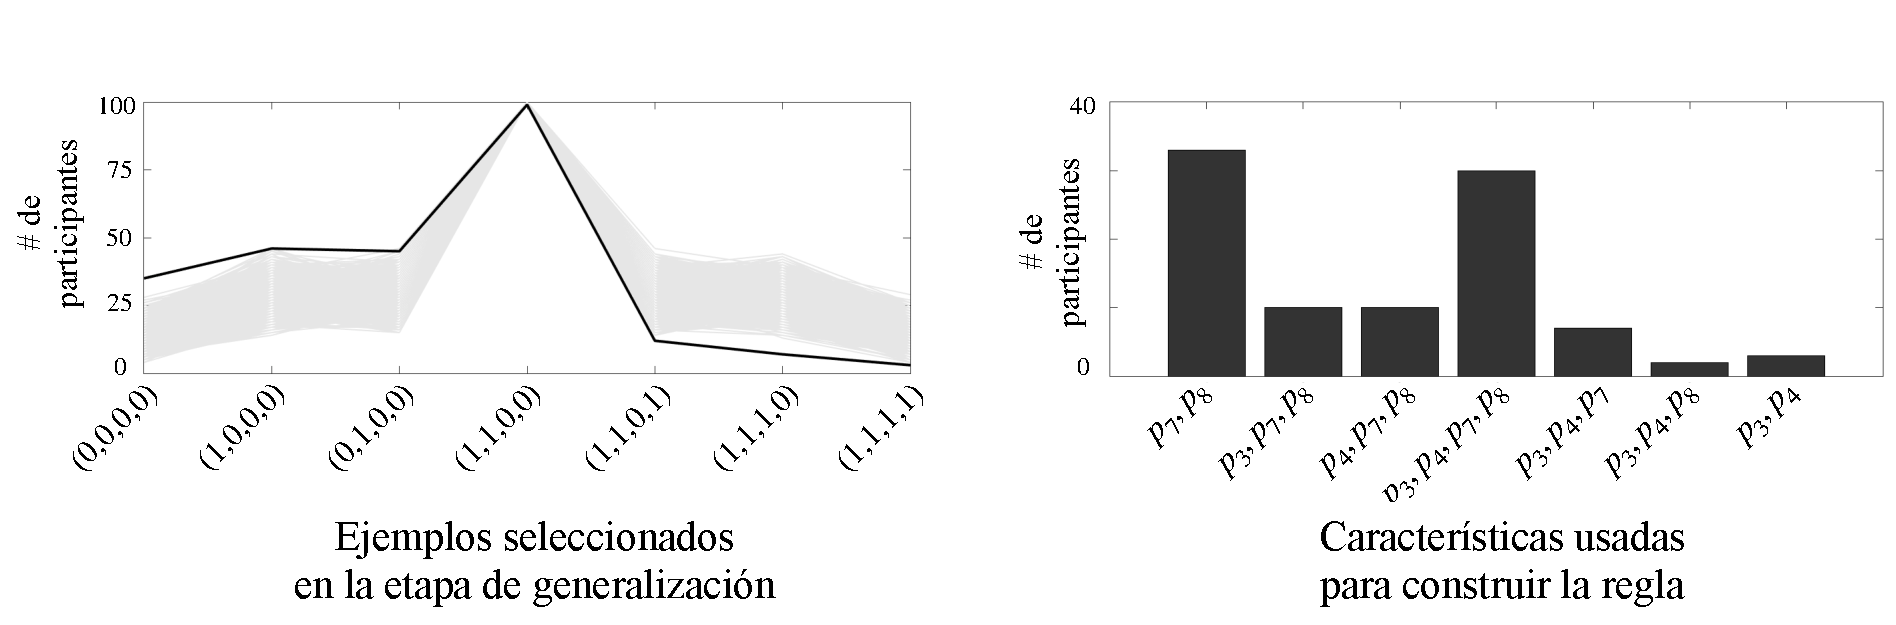
\includegraphics[scale=.4]{../figuras/brm/results_1_sp.pdf}
\end{center}\caption{
% \textbf{(Left)} Number of participants (100 participants total) that, in the generalization stage of Trial 6, selected an element (possibly among others; the numbers add up to more than 100) with the elements written on the x-axis, indicating the values of the features $\{p_3,p_4,p_7,p_8\}$ respectively. As multiple choices were possible, the sum for all choices adds up to a value greater than 100. In grey we show 100,000 simulations in which 100 agents randomly attend to one of the seven subset of features (see text). \textbf{(Right)} From the selected objects in the generalization phase we can infer which features participants used to build the rule for the concept (89 valid participants, see main text).
\textbf{(Izquierda)} Número de participantes (100 participantes en total) que, en la etapa de generalización de la Prueba 6, seleccionaron un elemento (posiblemente entre otros; los números suman más de 100) con los elementos escritos en el eje x, indicando los valores de las características $ \{p_3, p_4, p_7, p_8 \} $ respectivamente. Como eran posibles múltiples opciones, la suma de todas las opciones suma un valor mayor que 100. En gris mostramos 100.000 simulaciones en las que 100 agentes atienden aleatoriamente a uno de los siete subconjuntos de características (ver texto). \textbf{(Derecha)} De los objetos seleccionados en la fase de generalización podemos inferir qué características usaron los participantes para construir la regla para el concepto (89 participantes válidos, ver texto principal).
}
\label{fig:results1}
\end{figure}

 
\begin{figure}[h!]
\begin{center}
	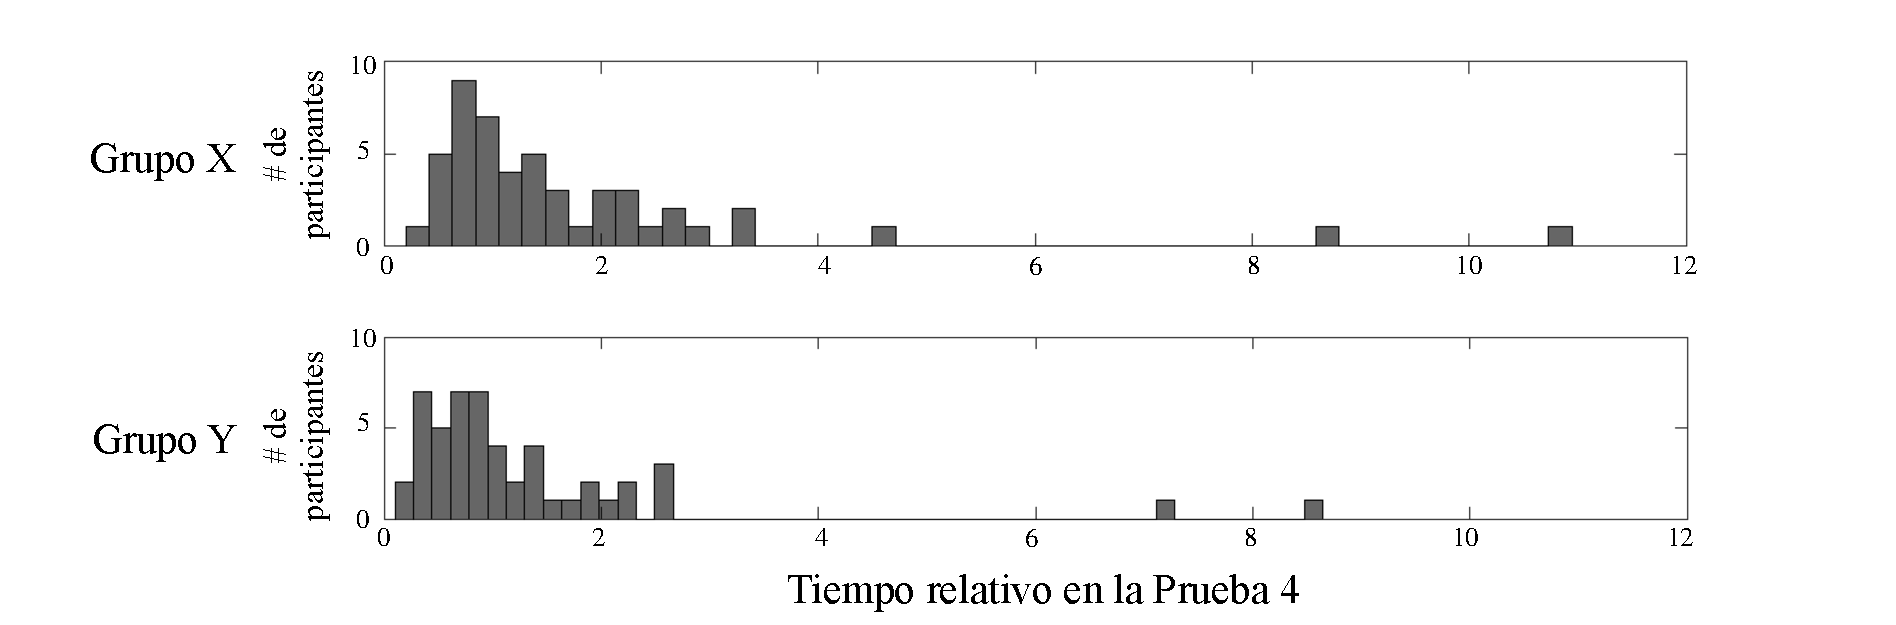
\includegraphics[scale=.5]{../figuras/brm/results_2_sp.pdf}
\end{center}
\caption{
% Relative time spent in Trial 4 by participants from the two groups, normalized by the time spent in Trial 5.
Tiempo relativo empleado en la Prueba 4 por los participantes de los dos grupos, normalizado por el tiempo empleado en la Prueba 5.
}
\label{fig:results2}
\end{figure}



% \subsection{Hypothesis \ref{Hip:FeatureBiasTimeAdvantage}}\label{Results:FeatureBiasTimeAdvantage} 
\subsection{Hipótesis \ref{Hip:FeatureBiasTimeAdvantage}}\label{Results:FeatureBiasTimeAdvantage} 

% This hypothesis regarded the behavioral advantage of the feature stickiness effect, which we tested by comparing learning \emph{times} in Trial 4 for participants of Groups X versus Y (see Figure~\ref{fig:results2}). If the feature stickiness bias represents a behavioral advantage, Group Y should learn concept $C^4_1$ \emph{faster} than Group X. To avoid confounds due to inter-individual differences in absolute learning time, for this analysis we normalize individual learning times with the time spent in Trial 5, which uses different features than the previous concepts and should not be affected by any obvious inter-trial relation with previous concepts\footnote{Indeed, Trial 5 was pre-registered as a `normalizer' trial.}. Thus we compare between the two groups (X and Y) the time spent in Trial 4 divided the time expended in Trial 5. This gives one number for each participant, and we compare the lists of numbers of the two groups using a two-sample t-test.  The differences in the learning times between the groups are not significant if we analyze the data of all participants as shown in Figure~\ref{fig:results2} (two-sample t-test shows $t_{98}=1.26 \ $,  $P=0.2$; Cohen's $d=0.25$), but they are significant if we rule out from this analysis 5 outliers that spent more than 5 times in concept 4 than 5, or in concept 5 than 4 ($t_{98}=2.18 \ $,  $P<0.05$, Cohen's $d=0.42$)\footnote{The ANOVA proposed in the pre-registration also did not reveal significant differences in learning times. For simplicity in the analysis of the outliers, we replaced here the ANOVA for a simple t-test between the normalized learning times of the two groups.}.
Esta hipótesis consideró la ventaja conductual del efecto de adherencia de características, que probamos comparando el tiempo de aprendizaje en la Prueba~4 para los participantes de los Grupos X versus Y (ver Figura~\ref{fig:results2}). Si el sesgo de adherencia de la característica representa una ventaja de comportamiento, el Grupo Y debería aprender el concepto $ C^4_1 $ \emph{más rápido} que el Grupo X. Para evitar confusiones debido a diferencias inter-individuales en el tiempo absoluto de aprendizaje, para este análisis normalizamos el tiempo de aprendizaje individual con el tiempo invertido en la Prueba 5, que utiliza características diferentes a los conceptos anteriores y no debería verse afectado por ninguna relación obvia entre pruebas con conceptos anteriores\footnote{De hecho, la Prueba 5 fue pre-registrada como una prueba `normalizadora'.}. Por lo tanto, comparamos entre los dos grupos (X e Y) el tiempo empleado en la Prueba 4 dividido el tiempo empleado en la Prueba 5. Esto da un número para cada participante, y comparamos las listas de números de los dos grupos usando un t-test de dos muestras. Las diferencias en los tiempos de aprendizaje entre los grupos no son significativas si analizamos los datos de todos los participantes, como se muestra en la Figura~\ref{fig:results2} (el t-test de dos muestras da $ t_{98} = 1.26 $, $ p = 0.2 $; $d$ de Cohen $= 0.25 $), pero sí son significativos si descartamos de este análisis 5 valores atípicos que gastaron más de 5 veces en el concepto 4 que en el 5, o en el concepto 5 que en el 4 ($ t_{98} = 2.18 $, $ p < 0.05 $, $ d$ de Cohen $= 0.42 $)\footnote{El ANOVA propuesto en el pre-registro tampoco reveló diferencias significativas en los tiempos de aprendizaje. Para simplificar el análisis de los valores atípicos, reemplazamos aquí el ANOVA por un t-test simple entre los tiempos de aprendizaje normalizados de los dos grupos.}.



% \subsection{Hypothesis \ref{Hip:StickinessFeatureOperator}} \label{Results:StickinessFeatureOperator} 
\subsection{Hipótesis \ref{Hip:StickinessFeatureOperator}} \label{Results:StickinessFeatureOperator} 

% The idea of this hypothesis is to test if participants prefer sticking to operators or sticking to features form one trial to the next. In this work we did not find conclusive evidence regarding this hypothesis. We suspect that the cause was an experimental setup that underestimated the strength of the bias favoring the $\AND$ operator over the $\OR$ operator. We found that 77 of the 100 participants explained Trial 1 using $\AND$, 11 explained it using $\OR$ and 12 selected elements in the generalization phase with no clear rationale. Of the 77 that used $\AND$, 64 also used $\AND$ in Trial 2, thus changing features but maintaining operator; and 7 of them used $\OR$, changing operator but maintaining features (the other 6 selected elements with no clear rationale). Of the 11 that used $\OR$, 10 used $\AND$ in Trial 2, changing operator but maintaining features; and 1 of them used $\OR$ in the second trial. We realize, however, that a change from using $\OR$ in the first concept to $\AND$ in the second one could not only be due to the effect of feature stickiness, but also simply to the stronger preference for $\AND$. Thus without a precise quantitative knowledge of the prior preference of $\AND$ over $\OR$, we cannot conclude about the effect of operator stickiness vs.\ feature stickiness. A future experiment could probe the existence of operator stickiness by having longer consecutive periods where feature reuse is not a useful bias and where only one logical operator remains useful for explaining a concept, before finally presenting a concept that can be explained via two different rules, each using different operators. Thus we leave for future work the task of studying the interaction between the feature stickiness bias and the precise structure of the logical rules being learnt. 
La idea de esta hipótesis es probar si, de una prueba a la siguiente, los participantes prefieren ceñirse a los operadores o ceñirse a las características. En este trabajo no encontramos evidencia concluyente sobre esta hipótesis. Sospechamos que la causa fue una configuración experimental que subestimó la fuerza del sesgo que favorecía al operador $ \AND $ sobre el operador $ \OR $. Encontramos que 77 de los 100 participantes explicaron la Prueba 1 usando $ \AND $, 11 lo explicaron usando $ \OR $ y 12 de ellos seleccionaron elementos en la fase de generalización sin una justificación clara. De los 77 que usaron $ \AND $, 64 también usaron $ \AND $ en la Prueba 2, cambiando así las características pero manteniendo el operador; y 7 de ellos usaron $ \OR $, cambiando de operador pero manteniendo las características (los otros 6 participantes seleccionaron elementos sin una justificación clara). De los 11 que usaron $ \OR $, 10 usaron $ \AND $ en la Prueba 2, cambiando de operador pero manteniendo las características; y 1 de ellos usó $ \OR $ en la segunda prueba. Sin embargo, nos damos cuenta de que un cambio de usar $ \OR $ en el primer concepto a $ \AND $ en el segundo podría deberse no solo al efecto de la adherencia de las características, sino también simplemente a la preferencia más fuerte por $ \AND$. Por lo tanto, sin un conocimiento cuantitativo preciso de la preferencia previa de $ \AND $ sobre $ \OR $, no podemos concluir nada sobre el efecto de la adherencia del operador frente a la adherencia de la característica. Un experimento futuro podría probar la existencia de adherencia de operador al tener períodos consecutivos más largos donde la reutilización de características no es un sesgo útil y donde solo un operador lógico sigue siendo útil para explicar un concepto, antes de presentar finalmente un concepto que se puede explicar a través de dos reglas diferentes, cada uno usando diferentes operadores.


% \subsection{MDL bias} \label{Resultados:MDLbias} 
\subsection{El sesgo de MDL} \label{Resultados:MDLbias} 


% The MDL-bias hypothesis posits that concept-learning difficulty increases with its MDL~\cite{feldman2000minimization}. In addition to their other roles, Trials 3 (group X and Y), 4, and 5 served to test this hypothesis in the new framework of multiple consistent explanations. In these trials, there were two possible explanations that were consistent with the shown data, one of much higher MDL than the other (15 vs.\ 3). For example, in the Group X of Trial~3, the short explanation was $p_1 \land p_2$, while the longer one was $((p_3 \lor (p_4 \lor p_5))\land(\lnot p_3 \lor ((p_4 \lor \lnot p_5)\land (p_5 \lor \lnot p_4))))$; the longer rule in other trials was always a substitution of features applied to this one (in order to keep the features disjoint between the two explanations). For these 3 trials, the responses of the $100$ participants add to a total of $300$ responses. From this total, $18$ responses in the generalization phase did not choose objects consistent with any of the two explanations; $2$ responses were consistent with the MDL~15 rule; and $280$ responses were consistent with the MDL~3 rule. While this was expected by the experimental design (since we included a MDL~15 rule in those trials where we wanted to bias the participants into finding the other rule), we conclude that the MDL-bias hypothesis holds in this framework of multiple consistent explanations. Future work could explore in greater detail the relative difficulty of rules with slightly different MDL in this framework.
La hipótesis del sesgo de MDL postula que la dificultad de aprendizaje de conceptos aumenta con su MDL~\cite{feldman2000minimization}. Además de sus otros roles, las Pruebas 3 (grupo X e Y), 4 y 5 sirvieron para testear esta hipótesis en el nuevo marco de múltiples explicaciones consistentes. En estas pruebas, hubo dos posibles explicaciones que eran consistentes con los datos mostrados, una de MDL mucho más alta que la otra (15 vs.\ 3). Por ejemplo, en el Grupo X de la Prueba~3, la explicación corta fue $ p_1 \land p_2 $, mientras que la más larga fue $ ((p_3 \lor (p_4 \lor p_5)) \land (\lnot p_3 \lor ( (p_4 \lor \lnot p_5) \land (p_5 \lor \lnot p_4)))) $; la regla más larga en otras pruebas fue siempre una sustitución de características aplicadas a esta última (para mantener las características disjuntas entre las dos explicaciones). Para estas 3 pruebas, las respuestas de los $ 100 $ participantes suman un total de $ 300 $ respuestas. De este total, las respuestas de $ 18 $ en la fase de generalización no eligieron objetos consistentes con ninguna de las dos explicaciones; $ 2 $ respuestas fueron consistentes con la regla de MDL~15; y $ 280 $ respuestas fueron consistentes con la regla de MDL~3. Si bien esto era lo esperable por el diseño experimental (dado que incluimos una regla de MDL~15 en aquellas pruebas en las que queríamos sesgar a los participantes para que encontraran la otra regla), concluimos que la hipótesis del sesgo de MDL se mantiene en este marco de múltiples explicaciones consistentes. 



% \section{Discussion}\label{sec:Discussion}
\section{Discusión}\label{sec:Discussion}


% In this work,  we  design  an experimental framework in which participants observe an incomplete set of examples, which are consistent with two alternative minimal descriptions depending on which features are observed.  We  illustrate  several advantages of our method compared to separately presenting sets of examples consistent with only one minimal description at a time. First, we  show  that when a set of examples is consistent with a disjunction \textit{and also} with a conjunction, participants are more likely to find the conjunction, in accordance with well-known previous results that show that the conjunction is learnt faster than the disjunction when presented separately~\cite{bourne1970knowing}. Then, we  show  that when rules of significantly different MDL are consistent with the observations, almost all participants discover the simpler rules, consistent with previous result showing that, when rules of different MDL are tested separately, learning times are proportional to MDLs~\cite{feldman2000minimization}. Finally, we  show  that when the logical structure of the minimal rules is independent of the selected features, participants are more likely to reuse the same features used to describe previous concepts,  and preliminary results suggest that reusing features  allows them to learn concepts faster than a control group that is not reusing features. To our knowledge this effect has not been previously characterized in the concept-learning literature, adding to the library of effects illustrating how human attention is biased towards features that are useful to describe the concepts (see~\cite{blair2009extremely,kruschke2000blocking,kruschke2005eye,hoffman2010costs}, among others).
En este trabajo, diseñamos un marco experimental en el que los participantes observan un conjunto incompleto de ejemplos, que son consistentes con dos descripciones mínimas alternativas según las características que se observen. Ilustramos varias ventajas de nuestro método en comparación con la presentación por separado de conjuntos de ejemplos consistentes con solo una descripción mínima a la vez. Primero, mostramos que cuando un conjunto de ejemplos es consistente con una disyunción \textit{y también} con una conjunción, es más probable que los participantes encuentren la conjunción, de acuerdo con resultados previos bien conocidos que muestran que la conjunción se aprende más rápido que la disyunción cuando se presentan por separado~\cite{bourne1970knowing}. Luego, mostramos que cuando las reglas con MDL significativamente diferentes son consistentes con las observaciones, casi todos los participantes descubren las reglas más simples, consistentes con el resultado anterior que muestra que, cuando las reglas con MDL diferentes se testean por separado, los tiempos de aprendizaje son proporcionales a las MDLs~\cite{feldman2000minimization}. Finalmente, mostramos que cuando la estructura lógica de las reglas mínimas es independiente de las características seleccionadas, es más probable que los participantes reutilicen las mismas características usadas para describir conceptos anteriores, y los resultados preliminares sugieren que la reutilización de características les permite aprender conceptos más rápido que un grupo de control que no está reutilizando características. Hasta donde sabemos, este efecto no se ha caracterizado previamente en la literatura sobre el aprendizaje de conceptos, lo que se suma a la biblioteca de efectos que ilustran cómo la atención humana está sesgada hacia características que son útiles para describir los conceptos (ver~\cite{blair2009extremely, kruschke2000blocking, kruschke2005eye, hoffman2010costs}, entre otros).


% Eye-tracking studies in categorization tasks have revealed that feature attention rapidly changes between trials depending on which features are relevant for classification in each trial~\cite{blair2009extremely}, as well as depending on prior knowledge about feature relevance~\cite{kim2011prior}. In~\cite{kruschke2005eye} it is found that eye movements confirmed that attention was learned in the basic learned inhibition paradigm, and in~\cite{hoffman2010costs} it is also found that eye movements revealed how an attention profile learned during a first phase of learning affected a second phase.  Our experimental setup allows us to test an arguably simpler complementary hypothesis: everything else being equal, participants are biased to use the same features used in the past.  Importantly, we were only able to test this hypothesis thanks to our framework, which allows us to present a set of examples consistent with two rules of exactly the same logical structure, but using different sets of features. Then, without using eye-tracking, we can recover which rule the participants learned, and thus which set of features they attended to. Since the two sets of features explain the examples using exactly the same logical structure, preferentially explaining the concept using one set of features over the other can only be due to a preference over the features themselves, and not a preference over alternative logical structures. 
Los estudios de seguimiento ocular ({\em eye tracking}) en tareas de categorización han revelado que la atención a las características cambia rápidamente entre pruebas dependiendo de qué características son relevantes para la clasificación en cada ensayo~\cite{blair2009extremely}, así como según el conocimiento previo sobre la relevancia de las características~\cite{kim2011prior}. En~\cite{kruschke2005eye} se mostró que los movimientos oculares confirmaron que la atención se puede aprender en el paradigma básico de inhibición aprendida, y en~\cite{hoffman2010costs} también se encontró que los movimientos oculares revelaron cómo un perfil de atención aprendido durante una primera fase de aprendizaje afectó una segunda fase. Nuestra configuración experimental nos permite probar una hipótesis complementaria posiblemente más simple: si todo lo demás permanece igual, los participantes están predispuestos a usar las mismas características que se usaron en el pasado. Es importante destacar que solo pudimos probar esta hipótesis gracias a nuestro marco, que nos permite presentar un conjunto de ejemplos consistentes con dos reglas de exactamente la misma estructura lógica, pero usando diferentes conjuntos de características. Luego, sin usar el seguimiento ocular, podemos recuperar qué regla aprendieron los participantes y, por lo tanto, a qué conjunto de características prestaron atención. Dado que los dos conjuntos de características explican los ejemplos usando exactamente la misma estructura lógica, explicar preferentemente el concepto usando un conjunto de características sobre el otro solo puede deberse a una preferencia sobre las características en sí mismas, y no una preferencia sobre estructuras lógicas alternativas.



% Although some of the hypothesis that we test are aligned with the well-known Einstellung effect which states that adopted solutions may hinder simpler ones when aiming at tackling novel problems, our experimental setting is different to the classical water jar test (the most commonly cited example of an Einstellung effect, where participants need to discover how to measure a certain amount of water using three jars with different and fixed capacity) ~\cite{luchins1942mechanization} in two senses. First, we do not drive the experiment to control and supervise the aspects that participants have to pay attention to. On the contrary, our focus is on the {\em choice} of the features that show to be useful for learning a concept with more than one rational explanation. Second, our experimental framework is consistent with the Language of Thought (\lot) hypothesis~\cite{fodor1975language}, which states that the human capacity to describe concepts —and, more generally, of all elements of thought— builds on the use of a symbolic and combinatorial mental language and it is specifically conceived to handle expressions in propositional Logic (but expansible to other formal languages), which is the ground where the rational explanations can be formalized. Such approach enables us to treat the notion of {\em feature} in a very precise way. 
Aunque algunas de las hipótesis que probamos están alineadas con el conocido efecto Einstellung, que establece que las soluciones adoptadas pueden obstaculizar las más simples al tratar de abordar problemas nuevos, nuestro entorno experimental es diferente a la prueba clásica de la jarra de agua (el ejemplo más comúnmente citado de un efecto Einstellung, donde los participantes necesitan descubrir cómo medir una cierta cantidad de agua usando tres jarras con capacidad diferente y fija)~\cite{luchins1942mechanization} en dos direcciones. Primero, no condujimos el experimento para controlar y supervisar los aspectos a los que los participantes deben prestar atención. Por el contrario, nuestro enfoque está en la {\em elección} de las características que demuestran ser útiles para aprender un concepto con más de una explicación racional. En segundo lugar, nuestro marco experimental es coherente con la hipótesis del \lot, y está específicamente concebido para manejar expresiones en lógica proposicional (pero expansible a otros lenguajes formales), que es el terreno donde se pueden formalizar las explicaciones racionales. Este enfoque nos permite tratar la noción de {\em característica} de una manera muy precisa.


% We note that other frameworks besides \lot can be used for our experiment. For example, consider similarity-based classification rules~\cite{juslin2003cue,juslin2003exemplar}, where each feature is multiplied by a weight and the classification rule is a function of the sum of the weighted features, usually a linear function with a soft decision boundary~\cite{juslin2003exemplar}. In this framework, the generalization phase would determine which of two possible decision boundaries was used by the participants (both consistent with the elements observed in the learning phase); and the feature-stickiness effect would be explained by the inertia of the weights' values from one concept to the next. However, two obstacles in this framework makes us prefer the \lot framework for Boolean concept-learning tasks. First, although a linear classification rule can readily learn the conjunctions and disjunctions in our experiment, more complex classification rules would require nonlinear functions of the features (e.g.\ the exclusive-or (XOR)). For nonlinear boundaries, the values of the weights that accompany the features could be hard to interpret, since it might no longer be true that a higher weight means higher feature importance. In contrast, in the \lot framework complex classification rules are compositionally built to accommodate concepts of any complexity, and feature importance can always be modeled as the probability of including a feature in a formula, independently of its complexity. Second, unlike similarity-based rules, the \lot framework naturally explains how humans can built verbal explanations for the learned concepts. Indeed, almost all participants gave informal explanations of conjunctions and disjunctions in propositional logic after learning each concept (see the shared data online for the list of verbal explanations). 
Observamos que se pueden utilizar otros marcos además de \lot para nuestro experimento. Por ejemplo, consideremos las reglas de clasificación basadas en similitudes~\cite{juslin2003cue, juslin2003exemplar}, donde cada característica se multiplica por un peso y la regla de clasificación es una función de la suma de las características ponderadas, generalmente una función lineal con un límite de decisión suave~\cite{juslin2003exemplar}. En este marco, la fase de generalización determinaría cuál de los dos posibles límites de decisión fue utilizado por los participantes (ambos consistentes con los elementos observados en la fase de aprendizaje); y el efecto de adherencia de características se explicaría por la inercia de los valores de los pesos de un concepto al siguiente. Sin embargo, dos obstáculos en este marco nos hacen preferir el marco de \lot para las tareas de aprendizaje de conceptos booleanos. Primero, aunque una regla de clasificación lineal puede aprender fácilmente las conjunciones y disyunciones en nuestro experimento, las reglas de clasificación más complejas requerirían funciones no lineales de las características (por ejemplo, el o-exclusivo ($\oxor$) analizado en el Capítulo~\ref{chapter:PRE}). Para los límites no lineales, los valores de las ponderaciones que acompañan a las características pueden ser difíciles de interpretar, ya que puede que ya no sea cierto que una ponderación más alta signifique una mayor importancia de las características. En contraste, en el marco de trabajo de \lot, las reglas de clasificación complejas se construyen de manera compositiva para acomodar conceptos de cualquier complejidad, y la importancia de las características siempre se puede modelar como la probabilidad de incluir una característica en una fórmula, independientemente de su complejidad. En segundo lugar, a diferencia de las reglas basadas en similitudes, el marco de \lot explica naturalmente cómo los humanos pueden construir explicaciones verbales para los conceptos aprendidos. De hecho, casi todos los participantes dieron explicaciones informales de conjunciones y disyunciones en la lógica proposicional después de aprender cada concepto (consultar los datos compartidos en línea para ver la lista de explicaciones verbales).


% Another well-studied phenomenon related to our work is Kamin’s cue {\em blocking}, where the learning of a given stimulus B is {\em blocked} by the mere fact that it was preceded by a set of stimuli A that already pairs with the outcome. This shows that the subject learned that stimulus B was not useful, and hence disregards their attention to it in the upcoming events~\cite{wagner1970stimulus,mackintosh1975theory,rescorlaw72}. Studied in humans in~\cite{chapman1990cue, arcediano1997blocking, kruschke2000blocking} among others, our work differs from these approaches in that we never introduce a stage were a feature A is intentionally exposed in absence to B, in order to guide the attention of the participant.
Otro fenómeno bien estudiado relacionado con nuestro trabajo es el {\em blocking} de Kamin, donde el aprendizaje de un estímulo B dado está {\em bloqueado} por el mero hecho de que fue precedido por un conjunto de estímulos A que ya se empareja con el resultado. Esto muestra que el sujeto aprendió que el estímulo B no era útil y, por lo tanto, ignora su atención en los eventos siguientes~\cite{wagner1970stimulus, mackintosh1975theory, rescorlaw72}. Estudiado en humanos en~\cite{chapman1990cue, arcediano1997blocking, kruschke2000blocking} entre otros, nuestro trabajo se diferencia de estos enfoques en que nunca introducimos una etapa donde una característica A se expone intencionalmente en ausencia de B, con el fin de orientar la atención del participante.


% We conjecture that most first-order determinants of subjective concept difficulty will also hold in a relative manner in our dual-concept setup, such as the MDL bias (for less extreme cases than evaluated in this work)~\cite{feldman2003simplicity} and the transfer learning hierarchical structure bias~\cite{tano2020towards}. Importantly, our experimental setup also allows to directly test second-order subjective difficulty effects (e.g.\ concept A is learnt faster if presented jointly with concept B than with concept C), as well as second-order transfer learning effects (e.g.\  participants learn more rapidly concept C if they have first observed concept A coupled with B$_1$, compared to A coupled with B$_2$). We believe that a systematic study of concept-learning difficulty with two (or more) concepts presented at the same time in each trial may open a new window into the dynamics of human concept-learning mechanisms. For example, consider the study in~\cite{piantadosi2016logical}, where participants gradually learn one concept while simultaneously selecting elements currently believed to belong to that concept. Here, the authors fit a Bayesian language model to participants' choices in order to illustrate how the posterior probability of the different rules in the grammar varied across time, to approximate the order in which different rules are learned. In contrast, using our experimental setting we can directly estimate, in a model-free manner, the probability that each rule is learnt faster than another. One simply needs to jointly present (in an incomplete and mutually compatible way) a set of examples consistent with those two minimal rules, and then measure the fraction of participants that discover each rule.
Conjeturamos que la mayoría de los determinantes de primer orden de la dificultad del concepto subjetivo también se mantendrán de manera relativa en nuestra configuración de concepto dual, como el sesgo de MDL (para casos menos extremos que los evaluados en este trabajo)~\cite{feldman2003simplicity} y el sesgo de la estructura jerárquica del aprendizaje por transferencia~\cite{tano2020towards}. Es importante destacar que nuestra configuración experimental también permite probar directamente los efectos de dificultad subjetiva de segundo orden (por ejemplo, el concepto A se aprende más rápido si se presenta junto con el concepto B que con el concepto C), así como los efectos de aprendizaje de transferencia de segundo orden (por ejemplo, los participantes aprenden más rápidamente el concepto C si primero han observado el concepto A junto con B$_1 $, en comparación con A junto con B$_2$). Creemos que un estudio sistemático de la dificultad de aprendizaje de conceptos con dos (o más) conceptos presentados al mismo tiempo en cada prueba puede abrir una nueva ventana a la dinámica de los mecanismos humanos de aprendizaje de conceptos. Por ejemplo, consideremos el estudio en~\cite{piantadosi2016logical}, donde los participantes aprenden gradualmente un concepto mientras simultáneamente seleccionan elementos que actualmente se creen que pertenecen a ese concepto. Aquí, los autores ajustan un modelo de lenguaje bayesiano a las elecciones de los participantes para ilustrar cómo la probabilidad a posteriori de las diferentes reglas en la gramática varió a lo largo del tiempo, para aproximar el orden en el que se aprenden las diferentes reglas. Por el contrario, utilizando nuestro entorno experimental podemos estimar directamente, sin modelos, la probabilidad de que cada regla se aprenda más rápido que otra. Uno simplemente necesita presentar conjuntamente (de una manera incompleta y mutuamente compatible) un conjunto de ejemplos consistentes con esas dos reglas mínimas, y luego medir la fracción de participantes que descubre cada regla.


% Usually, concept-learning biases have been studied in an isolated manner: the participant observes examples indicated as inside or outside a \textit{single} concept, and the experimenter evaluates its subjective difficulty for the participant. Although different methods have been used to present the concept to the participant (e.g.\ all elements at the same time~\cite{tano2020towards,kemp2012exploring} or small sets of elements presented in series~\cite{piantadosi2016logical}), to the best of our knowledge all previous category-learning studies have attempted to evaluate a single concept at a time. Here, we present a controlled logical setting to evaluate the relative difficulty of two concepts presented at the same time and under the same experimental conditions, and the framework could be generalized to more concepts straightforwardly. 
Por lo general, los sesgos de aprendizaje de conceptos se han estudiado de manera aislada: el participante observa ejemplos indicados como dentro o fuera de un concepto \textit{único}, y el experimentador evalúa su dificultad subjetiva para el participante. Aunque se han utilizado diferentes métodos para presentar el concepto al participante (por ejemplo, todos los elementos al mismo tiempo~\cite{tano2020towards, kemp2012exploring} o pequeños conjuntos de elementos presentados en serie~\cite{piantadosi2016logical}), por lo que está al alcance de nuestro conocimiento, todos los estudios previos de aprendizaje de categorías han intentado evaluar un solo concepto a la vez. Aquí, presentamos un escenario lógico controlado para evaluar la dificultad relativa de dos conceptos presentados al mismo tiempo y bajo las mismas condiciones experimentales, y, de forma directa, nuestro marco podría generalizarse a más de dos.



% \paragraph{Open Practices Statement.} 
\paragraph{Declaración de prácticas abiertas.} 
% This study's methodology, data collection procedures, sample size, exclusion criteria, and hypotheses were preregistered on the Open Science Framework (OSF) in advance of the data collection and analysis, in order to ensure transparency, reproducibility, and rigour. The preregistration of this study can be found at \url{https://osf.io/mgex3}. The actual experiment as presented to the participants, together with all the experimental data analyzed, is available online at \url{https://osf.io/gtuwp/}.
La metodología de este estudio, los procedimientos de recopilación de datos, el tamaño de la muestra, los criterios de exclusión y las hipótesis se registraron previamente en el Open Science Framework (OSF) antes de la recopilación y el análisis de datos, con el fin de garantizar la transparencia, la reproducibilidad y el rigor. El pre-registro de este estudio se puede encontrar en \url{https://osf.io/mgex3}. El experimento real presentado a los participantes, junto con todos los datos experimentales analizados, está disponible en línea en \url{https://osf.io/gtuwp/}.

%\bibliographystyle{apalike} 
%\bibliography{biblioCategorization}




    
Párrafo inicial retomando intro

En el capítulo \ref{chapter:BIN}, \textbf{una teoría de la memoria para secuencias binarias: evidencia de un algoritmo de compresión mental en humanos \cite{planton2021memory}}, pusimos a prueba la teoría de que los adultos humanos codifican secuencias binarias de estímulos en la memoria utilizando un \lot y un algoritmo de compresión recursivo a través de cinco experimentos compuestos por una variedad de secuencias auditivas y visuales. Proporcionamos una primera demostración de que, incluso después de tener en cuenta las probabilidades de transición, las respuestas a las violaciones de secuencia se pueden utilizar para descubrir las propiedades del lenguaje abstracto del pensamiento utilizado por los individuos para codificar patrones secuenciales. La propuesta de \grambin, que toma la forma de un lenguaje formal psicológicamente plausible compuesto por un conjunto restringido de reglas simples, demostró ser más eficaz que los enfoques alternativos en el modelado de la memoria humana para secuencias simples. La relación observada entre la complejidad de la secuencia, \mdlbin, y el desempeño en la detección de violaciones es coherente con la idea de que el cerebro actúa como un compresor de información entrante que captura regularidades y las usa para predecir el resto de la secuencia. El presente paradigma pasivo y no verbal allana el camino para futuros estudios de registros neurofisiológicos que podrían probar las similitudes y diferencias entre los humanos y otras especies~\cite{f13} o probar las habilidades de los bebés preverbales~\cite{f70}. Una pregunta fundamental para las investigaciones futuras es si el mismo lenguaje formal puede explicar el procesamiento de secuencias en otras especies de primates, o si tal lenguaje es exclusivo de los humanos~\cite{f6}.

Hemos discutido también en ese mismo capítulo si los resultados podrían estar sesgados dado que comenzamos con un \lot preconcebido y secuencias seleccionadas cuyas estructuras fueron bien capturadas por ese lenguaje (así como algunas secuencias que eran máximamente irregulares también según ese lenguaje). Si bien hemos planteado algunos argumentos que permiten descartar esa idea, profundizamos sobre este problema en el capítulo \ref{chapter:PO}, \textbf{validación bayesiana de producciones gramaticales para el \lot~\cite{romano2018bayesian}}, donde presentaremos un método de validación para los modelos \lot que permite tener mayores certezas sobre las reglas atómicas elegidas para construir los lenguajes. Aplicamos este método en el lenguaje \gramgeo, el \lot de secuencias geométricas sobre el que se basó \grambin, para distinguir entre las producciones originales y un conjunto de producciones ad-hoc arbitrarias. Finalmente, a pesar de que \gramgeo no es un lenguaje universal, mostramos una relación empírica entre la probabilidad de una secuencia y su complejidad, consistente con la relación teórica para los lenguajes universales descrita por el Teorema de codificación de Levin~\cite{levin1974laws}. Esto abre una oportunidad para cerrar la brecha entre los enfoques de \lot basados en métodos de longitud mínima de descripción y aquellos basados en modelos probabilísticos bayesianos.

En ambos trabajos de la parte I (así como en la mayoría de los estudios sobre \lot) el modelo elegido se fija una vez entrenado a partir de los datos, lo cual genera cierta inconsistencia con la extensa literatura que muestra cómo la experiencia da forma permanente al aprendizaje de conceptos. Por eso en el capítulo \ref{chapter:PRE}, \textbf{hacia un \lot más flexible: la gramática Bayesiana se actualiza después de cada exposición de conceptos~\cite{tano2020towards}}, realizamos un experimento para investigar la plasticidad del \lot. Definimos un modelo para medir la dificultad subjetiva de aprender una secuencia de conceptos lógicos. El modelo actualiza las probabilidades de producción gramaticales entre conceptos y predice la dificultad como el tamaño de las fórmulas compatibles ponderado por su probabilidad a posteriori. Este mecanismo de aprendizaje permite simular la aparición de una nueva primitiva en el lenguaje, ya que resulta útil para codificar los conceptos presentados hasta ese momento. Las dificultades predichas se asemejan mucho al patrón de los tiempos de aprendizaje humano en una secuencia de conceptos que requirieron el operador $ \oxor $ para ser representados de manera eficiente.

Finalmente, en el capítulo \ref{chapter:BRM}, \textbf{un marco lógico para estudiar los sesgos de aprendizaje de conceptos en presencia de múltiples explicaciones~\cite{tano2021framework}}, ampliamos el diseño experimental del capítulo anterior para desarrollar un marco experimental novedoso que permite presentar conceptos que son simultáneamente consistentes con dos o más reglas de diferente complejidad y que utilizan diferentes características para comparar, de forma directa y bajo las mismas condiciones experimentales, los sesgos de aprendizaje de conceptos. Explotamos el marco estudiado en un experimento con una secuencia de conceptos lógicos para ilustrar la aparición de sesgos conocidos y estudiados previamente, y de otros sesgos y efectos de transferencia caracterizados por primer vez. 

Párrafo final cerrando.
    %%!TEX root = ../main.tex

%\section*{Abstract}
%Probabilistic proposals of Language of Thoughts (LoTs) can explain learning across different domains as statistical inference over a compositionally structured hypothesis space. While frameworks may differ on how a LoT may be implemented computationally, they all share the property that they are built from a set of atomic symbols and rules by which these symbols can be combined.
%In this work we propose an extra validation step for the set of atomic productions defined by the experimenter. It starts by expanding the defined LoT grammar for the cognitive domain with a broader set of arbitrary productions and then uses Bayesian inference to prune the productions from the experimental data. The result allows the researcher to validate that the resulting grammar still matches the intuitive grammar chosen for the domain. We then test this method in the \textit{language of geometry}, a specific LoT model for geometrical sequence learning. Finally, despite the fact of the geometrical LoT not being a universal (i.e. Turing-complete) language, we show an empirical relation between a sequence's {\em probability} and its {\em complexity} consistent with the theoretical relationship for universal languages described by Levin's Coding Theorem.

\chapter{BORRAR: Validación bayesiana de producciones gramaticales para el lenguaje del pensamiento}\label{chapter:PO}
\chaptermark{Validación bayesiana de gramáticas}

\section{Introducción}

%\blockquote{It was not only difficult for him to understand that the generic term dog embraced so many unlike specimens of differing sizes and different forms; he was disturbed by the fact that a dog at three-fourteen (seen in profile) should have the same name as the dog at three-fifteen (seen from the front). (...)With no effort he had learned English, French, Portuguese and Latin. I suspect, however, that he was not very capable of thought. To think is to forget differences, generalize, make abstractions. In the teeming world of Funes, there were only details, almost immediate in their presence. \cite{funes}}

\blockquote{No sólo le costaba comprender que el símbolo genérico perro abarcara tantos individuos dispares de diversos tamaños y diversa forma; le molestaba que el perro de las tres y catorce (visto de perfil) tuviera el mismo nombre que el perro de las tres y cuarto (visto de frente) (...) Había aprendido sin esfuerzo el inglés, el francés, el portugués, el latín. Sospecho, sin
embargo, que no era muy capaz de pensar. Pensar es olvidar diferencias, es generalizar, abstraer. En el abarrotado mundo de Funes no había sino detalles, casi inmediatos. \cite{funes}}

%In his fantasy story, the writer Jorge Luis Borges described a fictional character, Funes, capable of remembering every detail of his life but not being able to generalize any of that data into mental categories and hence --Borges stressed-- not capable of thinking.

En su cuento, el escritor Jorge Luis Borges describió a un personaje de ficción, Fines, capaz de recordar cada detalle de su vida, pero sin ser capaz de generalizar ninguna de esa información en categorías mentales y, por tanto --recalcó Borges--, incapaz de pensar.

%Researchers have modeled these mental categories or conceptual classes with two classical approaches: in terms of similarity to a generic example or prototype \cite{rosch1999principles,nosofsky1986attention,rosch1976structural,rosch1975family} or based on a symbolic/rule-like representation \cite{boole1854investigation,fodor1975language,gentner1983structure}.

Los investigadores han modelado estas categorías mentales o clases conceptuales con dos enfoques clásicos: en términos de su similitud con un ejemplo genérico o prototipo \cite{rosch1999principles,nosofsky1986attention,rosch1976structural,rosch1975family} o basados en una representación simbólica a través de reglas  \cite{boole1854investigation,fodor1975language,gentner1983structure}.

%Symbolic approaches like the \textit{language of thought} (LoT) hypothesis \cite{fodor1975language}, claim that thinking takes form in a sort of mental language, composed of a limited set of atomic symbols that can be combined to form more complex structures following combinatorial rules.

Enfoques simbólicos como la hipótesis del \textit{lenguaje del pensamiento} (LoT, por sus siglas en inglés) \cite{fodor1975language}, afirman que el pensamiento toma forma en una especie de lenguaje mental compuesto por un conjunto limitado de símbolos atómicos que se pueden combinar para formar estructuras más complejas siguiendo reglas combinatorias.

%Despite criticisms and objections \cite{blackburn1984spreading,loewer1991meaning,knowles1998language,aydede1997language}, symbolic approaches ---in general--- and the LoT hypothesis ---in particular--- have gained some renewed attention with recent results that might explain learning across different domains as statistical inference over a compositionally structured hypothesis space \cite{tenenbaum2011grow,piantadosi2016four}.

A pesar de las críticas y objeciones \cite{blackburn1984spreading,loewer1991meaning,knowles1998language,aydede1997language}, los enfoques simbólicos ---en general--- y la hipótesis LoT ---en particular--- han ganado una atención renovada con resultados recientes que podrían explicar el proceso de aprendizaje en diferentes dominios como un proceso de inferencia estadística sobre un espacio de hipótesis estructurado y componible \cite{tenenbaum2011grow,piantadosi2016four}.

%The LoT is not necessarily unique. In fact, the form that it takes has been modeled in many different ways depending on the problem domain: numerical concept learning \cite{piantadosi2012bootstrapping}, sequence learning \cite{marie2016,yildirim2015learning,romano2013language}, visual concept learning \cite{ellis2015unsupervised}, theory learning \cite{ullman2012theory}, etc.

El Lot no es necesariamente único. De hecho, la forma que toma ha sido modelada de muchas formas diferentes diferentes dependiendo del dominio del problema: aprendizaje de conceptos numéricos \cite{piantadosi2012bootstrapping}, aprendizaje de secuencias \cite{marie2016,yildirim2015learning,romano2013language}, aprendizaje visual de conceptos \cite{ellis2015unsupervised}, aprendizaje de teorías \cite{ullman2012theory}, etc.

%While frameworks may differ on how a LoT may be implemented computationally, they all share the property of being built from a set of atomic symbols and rules by which they can be combined to form new and more complex expressions.

Si bien los trabajos pueden diferir en cómo se puede implementar un LoT computacionalmente, todos comparten la propiedad de estar construidos a partir de un conjunto de símbolos atómicos y reglas por las que se los pueden combinar para formar expresiones nuevas y más complejas.

%Most studies of LoTs have focused on the compositional aspect of the language, which has either been modeled within a Bayesian \cite{tenenbaum2011grow} or a Minimum Description Length (MDL) framework \cite{marie2016,goldsmith2002probabilistic,romano2013language,goldsmith2001unsupervised}.

La mayoría de los estudios de LoT se han centrado en el aspecto compositivo del lenguaje, modelando la composición a través de técnicas de probabilidad Bayesiana \cite{tenenbaum2011grow} o de longitud mínima de descripción (MDL, por sus siglas en inglés) \cite{marie2016,goldsmith2002probabilistic,romano2013language,goldsmith2001unsupervised}.

%The common method is to define a grammar with a set of productions based on operations that are intuitive to researchers and then study how different inference processes match regular patterns in human learning. A recent study \cite{piantadosi2016logical} puts the focus on the process of how to empirically choose the set of productions and how different LoT definitions can create different patterns of learning. Here, we move along that direction but use Bayesian inference to individuate the LoT instead of comparing several of them by hand.


El método más común es definir una gramática con un conjunto de producciones basadas en operaciones que son intuitivas para los investigadores y luego estudiar cómo diferentes procesos de inferencia coinciden con los patrones del aprendizaje humano. Un estudio reciente \cite{piantadosi2016logical} pone el foco en el proceso de cómo elegir empíricamente el conjunto de producciones y cómo diferentes definiciones del LoT pueden crear diferentes patrones de aprendizaje. En este trabajo, nos vemos en esa dirección pero utilizando la inferencia Bayesiana para seleccionar el LoT en lugar de seleccionarlo a partir de la comparación empírica de las distintas versiones con los patrones a replicar.

%Broadly, our aim is to propose a method to select the set of atomic symbols in an inferential process by pruning and trimming from a broad repertoire. More precisely, we test whether Bayesian inference can be used to decide the proper set of productions in a LoT defined by a context free grammar. These productions are derived from the subjects' experimental data. In order to do this, a researcher builds a broader language with two sets of productions: 1) those for which she has a strong prior conviction that they should be used in the cognitive task, and 2) other productions that could be used to structure the data and extract regularities even if she believes are not part of the human reasoning repertoire for the task. With the new broader language, she should then turn the context free grammar that defines it into a probabilistic context free grammar (PCFG) and use Bayesian analysis to infer the probability of each production in order to choose the set that best explains the data.

En términos generales, nuestro objetivo es proponer un método para seleccionar el conjunto de símbolos atómicos en un proceso de inferencia seleccionando y recortándolos de un repertorio más amplio. Más precisamente, nos interesa probar si la inferencia Bayesiana puede utilizarse para decidir el conjunto adecuado de producción en un LoT definido por una gramática libre de contexto, derivando las producciones a elegir de los datos experimentales de los sujetos del experimento. Para hacer esto, un investigador debería construir un lenguaje más amplio con dos conjuntos de producciones: 1) aquellas para las que tiene una fuerte convicción previa de que podrían ser utilizadas en la tarea cognitiva a estudiar, y 2) otras producciones que podrían utilizarse para estructurar los datos y extraer regularidades incluso si cree que no son parte del repertorio de razonamiento humano para la tarea. Con el nuevo lenguaje más amplio, debería convertir la gramática libre de contexto que lo define en una gramática probabilística libre de contexto (PCFG, por sus siglas en inglés) y utilizar en análisis Bayesiano para inferir probabilidad de cada producción y el conjunto que mejor explique los datos.

%In the next section we formalize this procedure and then apply it on the \textit{language of geometry} presented by Amalric et al. in a recent study about geometrical sequence learning \cite{marie2016}. This LoT defines a language with some basic geometric instructions as the grammar productions and then models their composition within the MDL framework. Our method, however, can be applied to any LoT model that defines a grammar, independently of whether its compositional aspect is modeled using a Bayesian framework or a MDL approach.

En la siguiente sección, formalizaremos este procedimiento y luego lo aplicaremos en el \textit{lenguaje de geometría} presentado por Amalric et al. en un reciente estudio sobre el aprendizaje de secuencias geométricas \cite{marie2016}. Este LoT define un lenguaje con algunos elementos geométricos básicos, con instrucciones como las producciones gramaticales y luego modela su composición dentro del marco de MDL. Nuestro método, sin embargo, se puede aplicar a cualquier modelo de LoT que defina una gramática, independientemente de si su aspecto compositivo se modela utilizando un enfoque de probabilidad Bayesiana o de MDL.

%Finally, even with the recent surge of popularity of Bayesian inference and MDL in cognitive science, there are --to the best of our knowledge-- no practical attempts to close the gap between probabilistic and complexity approaches to LoT models.

Finalmente, incluso con el reciente aumento de popularidad de la inferencia Bayesiana y el MDL en la ciencia cognitiva, no hay --- hasta donde sabemos---, intentos prácticos de cerrar la brecha entre ambos enfoques.

%The theory of computation, through Levin's Coding Theorem \cite{levin1974laws}, exposes a remarkable relationship between the {\em Kolmogorov complexity} of a sequence and its {\em universal probability}, largely used in algorithmic information theory. Although both metrics are actually non-computable and defined over a universal prefix Turing Machine, we can apply both ideas to other non-universal Turing Machines in the same way that the concept of complexity used in MDL can be computed for specific, non-universal languages.

La teoría de la computabilidad, a través del Teorema de Codificación de Levin \cite{levin1974laws}, expone una notable relación entre la {\em complejidad de Kolmogorov} de una secuencia (que es la base del cálculo del MDL) y su {\em probabilidad universal}, la cual es ampliamente utilizada en la teoría algorítmica de la información. Aunque ambas métricas resultan no computables y se encuentran definidas sobre una Máquina Universal de Turing libre de prefijos, podemos aplicar estas ideas a otras Máquinas de Turing no universales de la misma manera que el concepto de complejidad es utilizado para el cálculo de MDL en lenguajes específicos no universales. 

%In this work, we examine the extent to which this theoretical prediction for infinite sequences holds empirically for a specific LoT, the \textit{language of geometry}. Although the inverse logarithmic relationship between both metrics is proved for universal languages in the Coding Theorem, testing this same property for a particular non-universal language shows that the language shares some interesting properties of general languages. This constitutes a first step towards a formal link between probability and complexity modeling frameworks for LoTs.

En este trabajo también examinamos hasta qué punto esta predicción teórica para secuencias infinitas se preserva empíricamente para un LoT específico, el \textit{lenguaje de geometría}. Aunque la relación logarítmica inversa entre ambas métricas está probada para lenguas universales en el Teorema de Codificación, probar esta misma propiedad para un lenguaje no universal particular muestra que el lenguaje comparte algunas propiedades interesantes con los lenguajes generales. Esto constituye un primer paso hacia un vínculo formal entre el modelado de probabilidad y el de complejidad para el LoT.

%\section{Bayesian inference for LoT's productions}
\section{Inferencia Bayesiana para las producciones del LoT}

%The project of Bayesian analysis of the LoT models concept learning using Bayesian inference in a grammatically structured hypothesis space \cite{goodman2008rational}. Each LoT proposal is usually formalized by a context free grammar $\gram$ that defines the valid functions or programs that can be generated, like in any other programming language. A program is a derivation tree of $\gram$ that needs to be interpreted or executed according to a given semantics in order to get an actual description of the concept in the cognitive task at hand. Therefore, each concept is then represented by any of the programs that describe it and a Bayesian inference process is defined in order to infer from the observed data the distribution of valid programs in $\gram$ that describes the concepts.

El proyecto de análisis Bayesiano del LoT modela el aprendizaje de conceptos utilizando la inferencia Bayesiana en un espacio de hipótesis estructurado a partir de una gramática \cite{goodman2008rational}. Cada propuesta de LoT suele formalizarse mediante una gramática libre de contexto $\gram$ que define las funciones o programas válidos que se pueden generar, como en cualquier otro lenguaje de programación. Aquí, un programa es un árbol de derivación de $\gram$ que necesita ser interpretado o ejecutado de acuerdo a una semántica dada para obtener una descripción real del concepto en la tarea cognitiva en cuestión. Por lo tanto, cada concepto puede ser representado por cualquiera de los programas que lo describen al ejecutarse, y un proceso de inferencia Bayesiano es definido para calcular la distribución de los programas válidos de $\gram$ que describen los conceptos a explicar.

%As explained above, our aim is to derive the productions of $\gram$ from the data, instead of just conjecturing them using a priori knowledge about the task. Prior work on LoTs has fit probabilities of productions in a context free grammar using Bayesian inference, however, the focus has been put in integrating out the production probabilities to better predict the data without changing the grammar definition \cite{piantadosi2016logical}. Here, we want to study if the inference process could let us decide which productions can be safely pruned from the grammar. We introduce a generic method that can be used on any grammar to select and test the proper set of productions. Instead of using a fixed grammar and adjusting the probabilities of the productions to predict the data, we use Bayesian inference to rule out productions with probability lower than a certain threshold. This allows the researcher to validate the adequacy of the productions she has chosen for the grammar or even define one that is broad enough to express different regularities and let the method select the best set for the observed data.

Como se explicó anteriormente, nuestro objetivo es derivar las producciones de $\gram$ a partir de los datos, en lugar de sólo conjeturarlas utilizando un conocimiento a priori sobre la tarea. Otros trabajos previos en LoT ajustaron las probabilidades de las producciones de las gramáticas libres de contexto utilizando inferencia Bayesiana \cite{piantadosi2016logical}, sin embargo, han puesto el foco en la integración de las probabilidades de producción para predecir mejor los datos y no en cambiar la definición de las gramáticas. Aquí queremos estudiar si el proceso de inferencia podría permitirnos decidir qué producciones de la gramática pueden podarse con seguridad. Para esto, introducimos un método genérico que puede utilizarse en cualquier gramática para seleccionar y probar el conjunto adecuado de producciones. En lugar de usar una gramática fija y ajustar las probabilidades de las producciones para predecir los datos, utilizamos la inferencia Bayesiana para remover las producciones con una probabilidad inferior a cierto umbral. Esto permite al investigador validar lo adecuado de las producciones que ha elegido para la gramática o incluso definir una que sea lo suficientemente amplia como para expresar diferentes regularidades y dejar que el método seleccione el mejor conjunto a partir de los datos observados.   

%To infer the probability for each production based on the observed data, we need to add a vector of probabilities $\theta$ associated with each production in order to convert the context free grammar $\gram$ into a probabilistic context free grammar (PCFG) \cite{manning1999foundations}.

Para inferir la probabilidad de cada producción a partir de los datos observados, necesitamos agregar un vector de probabilidades $\theta$ asociado con cada producción para convertir a la gramática libre de contexto $\gram$ en una gramática probabilística libre de contexto (PCFG) \cite{manning1999foundations}.

%Let $D = (d_1, d_2, \dots, d_n)$ denote the list of concepts produced by the subjects in an experiment. This means that each $d_i$ is a concept produced by a subject in each trial. Then, $P(\theta \mid D)$, the posterior probability of the weights of each production after the observed data, can be calculated by marginalizing over the possible programs that compute $D$:

Sea $D = (d_1, d_2, \dots, d_n)$ la lista de conceptos producidos por los sujetos en un experimento. Esto significa que cada $d_i$ es un concepto producido por un sujeto en cada ensayo. Luego, $P(\theta \mid D)$, la probabilidad a posteriori de los pesos de cada producción después de observar los datos, se puede calcular marginalizando sobre los posibles programas que computan $D$:

%
\begin{equation}
\label{eqA}
P(\theta \mid D) = \sum_{\Prog} P(\Prog,\theta \mid D),
\end{equation} donde cada $\Prog  = (p_1, p_2, \cdots, p_n)$ es un posible conjunto de programas tales que cada $p_i$ computa el correspondiente concepto $d_i$.
%where each $\Prog  = (p_1, p_2, \cdots, p_n)$ is a possible set of programs such that each $p_i$ computes the corresponding concept $d_i$.

%We can use Bayesian inference to learn the corresponding programs $\Prog$ and the vector $\theta$ for each production in the grammar, applying Bayes rule in the following way:
Podemos usar la inferencia Bayesiana para aprender los programas correspondientes $\Prog$ y el vector $\theta$ para cada producción de la gramática, aplicando la regla de Bayes de la siguiente manera:
%
\begin{equation}
\label{eq:mainB}
P(\Prog,\theta \mid D) \propto P(D \mid \Prog)\ P(\Prog \mid \theta)\ P(\theta),
\end{equation}
%

%Sampling the set of programs from $P(\Prog \mid \theta)$ forces an inductive bias which is needed to handle uncertainty under sparse data. Here we use a standard prior for programs that is common in the LoT literature to introduce a syntactic complexity bias that favors shorter programs \cite{goodman2008rational,overlan2017learning}. Intuitively, the probability of sampling a certain program is proportional to the product of the production rules that were used to generate such program, and therefore inversely proportional to the size of the derivation tree. Formally, it is defined as:

Muestrear el conjunto de programas de $P(\Prog \mid \theta)$ fuerza un sesgo inductivo que es necesario para manejar la incertidumbre frente a datos escasos. Aquí usamos un estándar previo para los programas que es común en la literatura de LoT para introducir un sesgo de complejidad sintáctica que favorece programas más cortos \cite{goodman2008rational,overlan2017learning}. Intuitivamente, la probabilidad de muestreo de un determinado programa es proporcional al producto de las reglas de producción que se utilizaron para generar dicho programa y, por lo tanto, inversamente proporcional al tamaño del árbol de derivación. Formalmente, se define como:

%
\begin{equation}
\label{eqC}
P(\Prog \mid \theta)\ = \prod\limits_{i = 1}^n P(p_i \mid \theta),
\end{equation}
%
donde $P(p_i \mid \theta) = \prod\limits_{r \in G} \theta^{f_r(p_i)}_{r}$ es la probabilidad del programa $p_i$ en la gramática, y $f_r(p_i)$ es el número de ocurrencias de la producción $r$ en el programa $p_i$.
%where $P(p_i \mid \theta) = \prod\limits_{r \in G} \theta^{f_r(p_i)}_{r}$ is the probability of the program $p_i$ in the grammar, and $f_r(p_i)$ is the number of occurrences of the production $r$ in program $p_i$.

%In \eqref{eq:mainB}, $P(\theta)$ is a Dirichlet prior over the productions of the grammar. By using the term $P(\theta)$ we are abusing notation for simplicity. The proper term would be $P(\theta \mid \alpha)$ to express a Dirichlet prior with $\alpha \in \mathbb{R}^\ell$ its associated concentration vector hyper-parameter where $\ell$ is the number of productions in the grammar. This hierarchical Dirichlet prior has sometimes been replaced with a uniform prior on productions as it shows no significant differences in prediction results \cite{piantadosi2012bootstrapping,yildirim2015learning}. However, here we will use the Dirichlet prior to be able to infer the production probabilities from this more flexible model.

En \eqref{eq:mainB}, $P(\theta)$ es una Dirichlet que se utiliza como distribución a priori sobre las producciones de la gramática. Al utilizar el término $P(\theta)$ estamos abusando de la notación por simplicidad. El término adecuado sería $P(\theta \mid \alpha)$ para expresar la distribución a priori con $\alpha \in \mathbb{R}^\ell$ su hiperparámetro que actúa como vector de concentración asociado donde $\ell$ es el número de producciones de la gramática. Esta distribución a proiri ha sido también reemplazada por una distribución uniforme, ya que no muestra diferencias significativas en resultados de predicción \cite{piantadosi2012bootstrapping,yildirim2015learning}. Sin embargo, aquí utilizaremos la distribución Dirichlet para poder inferir las probabilidades de producción a partir de este modelo más flexible.

%The likelihood function is straightforward. It does not use any free parameter to account for perception errors in the observation. This forces that only programs that compute the exact concept are taken into account, and it can be easily calculated as follows:

La función de verosimilitud es sencilla. No utiliza ningún parámetro libre para contabilizar errores de percepción en la observación. Esto obliga a que sólo los programas que computan el concepto exacto se tengan en cuenta, y puede ser fácilmente calculada de la siguiente manera:
\begin{equation}
\label{eqD}
P(D \mid \Prog)\ = \prod\limits_{i = 1}^n P(d_i \mid p_i),
\end{equation}
donde $P(d_i \mid p_i) = 1 $ si el programa $p_i$ computa $d_i$, y 0 en caso contrario.
%where $P(d_i \mid p_i) = 1 $ if the program $p_i$ computes $d_i$, and 0 otherwise.

%Calculating $P(\theta \mid D)$ directly is, however, not tractable since it requires to sum over all possible combinations of programs $\Prog$ for each of the possible values of $\theta$. To this aim, then, we used a Gibbs Sampling \cite{geman1984stochastic} algorithm for PCFGs via Markov Chain Monte Carlo (MCMC) similar to the one proposed at \cite{johnson2007bayesian}, which alternates in each step of the chain between the two conditional distributions:

Sin embargo, calcular $P(\theta \mid D)$ de manera directa no es manejable ya que requiere sumar todas las posibles combinaciones de programas $\Prog$ para cada uno de los posibles valores de $\theta$. Para este objetivo, utilizamos entonces el algoritmo de muestreo de Gibbs \cite{geman1984stochastic} para PCFGs a través del Método de Monte Carlo basado en cadenas de Markov (MCMC, por sus siglas en inglés) similar al propuesto en \cite{johnson2007bayesian}, el cual alterna en cada paso de la cadena entre las dos distribuciones condicionales:
%
\begin{eqnarray}
\label{eqE}
P(\Prog \mid \theta, D) &=& \prod\limits_{i=1}^n P(p_i \mid d_i, \theta).\\
P(\theta \mid \Prog, D) &=& P_D(\theta \mid f(\Prog) + \alpha).
\end{eqnarray}
%Here, $P_D$ is the Dirichlet distribution where the positions of the vector $\alpha$ were updated by counting the occurrences of the corresponding productions for all programs $p_i \in \Prog$.
Aquí, $P_D$ es la distribución Dirichlet donde las posiciones del vector $\alpha$ fueron actualizadas contando las ocurrencias de las producciones correspondientes para todos los programas $p_i \in \Prog$.

%In the next section, we apply this method to a specific LoT. We add a new set of ad-hoc productions to the grammar that can explain regularities but are not related to the cognitive task. Intuitively, these ad-hoc productions should not be part of the human LoT repertory, still all of them can be used in many possible programs to express each concept.

En la siguiente sección, aplicamos este método a un LoT específico. Agregamos un nuevo conjunto ad-hoc de producciones a la gram'atica original que puedan explicar regularidades pero que no están relacionadas con la tarea cognitiva. Intuitivamente, estas producciones ad-hoc no deberían formar parte del repertorio del LoT, aún así, todas ellas pueden usarse en muchos programas posibles para expresar cada uno de los conceptos.

%So far, Probabilistic LoT approaches have been successful to model concept learning from few examples \cite{tenenbaum2011grow,piantadosi2016four}. However, this does not mean that Bayesian models would be able to infer the syntax of the model's grammar from sparse data. Here we test such hypothesis. If the method is effective, it should assign a low probability to the ad-hoc productions and instead favor the original set of productions selected by the researchers for the cognitive task. This would not only provide additional empirical evidence about the adequacy of the choice of the original productions for the selected LoT but, more importantly, about the usefulness of Bayesian inference for validating the set of productions involved in different LoTs.

Hasta ahora, los enfoques probabilísticos del LoT han tenido éxito para modelar el aprendizaje de conceptos a partir de pocos ejemplos \cite{tenenbaum2011grow,piantadosi2016four}. Sin embargo, esto no significa que los modelos Bayesianos puedan inferir la sintaxis de la gramática a partir de datos escasos. Aquí probamos esta hipótesis. Si el método es eficaz, debería asignar una probabilidad baja las producciones ad-hoc y en su lugar favorecer el conjunto original de producciones seleccionadas por los investigadores para la tarea cognitiva. Esto no sólo proporcionaría evidencia empírica adicional sobre la idoneidad de la elección original de producciones para el LoT, sino que ---más importante--- brindaría evidencia sobre la utilidad de la inferencia Bayesiana para validar el conjunto de producciones involucradas en diferentes LoTs. 

%\section{The Language of Geometry: $\geom$}
\section{El lenguaje de geometría: $\geom$}

%The \textit{language of geometry}, $\geom$ \cite{marie2016}, is a probabilistic generator of sequences of movements on a regular octagon like the one in \figref{fig:circle}. It has been used to model human sequence predictions in adults, preschoolers, and adult members of an indigene group in the Amazon. As in other LoT domains, different models have been proposed for similar spatial sequence domains like the one in \cite{yildirim2015learning}. Although both successfully model the sequences in their experiments, they propose different grammars for their models (in particular, \cite{marie2016} contains productions for expressing symmetry reflections). This difference can be explained by the particularities of each experiment. On the one hand, \cite{marie2016} categorized the sequences in 12 groups based on their complexity, displayed them in an octagon and evaluate the performance of a diverse population to extrapolate them. On the other hand, \cite{yildirim2015learning} categorized the sequences in 4 groups, displayed them in an heptagon and evaluate the performance of adults not just to predict how the sequence continues, but to transfer the knowledge from the learned sequence across auditory and visual domains. Despite the domains not being equal, the differences in the grammars strengths the need for automatic methods to test and validate multiple grammars for the same domain in the LoT community.

El \textit{lenguaje de geometría}, $\geom$ \cite{marie2016}, es un generador probabilístico de secuencias de movimientos en un octágono regular como el de la figura \figref{fig:circle}. Se ha usado para modelar predicciones de secuencias humanas en adultos y preescolares de Francia y miembros adultos de un grupo indígena en la Amazonia. Como en otros dominios de LoT, se han propuesto para el dominio de secuencias espaciales diferentes modelos como el de \cite{yildirim2015learning}. Aunque ambos modelan con éxito las secuencias en sus experimentos, proponen diferentes gramáticas para sus modelos (en particular, \cite{marie2016} contiene producciones para expresar reflexiones o simetrías). Esta diferencia se puede explicar por las particularidades de cada experimento. Por un lado, en \cite{marie2016} categorizaron secuencias en 12 grupos en función de su complejidad, mostrándolos en un octágono y evaluando el desempeño en una población diversa para extrapolar las secuencias. Por otro lado, en \cite{yildirim2015learning} categorizaron las secuencias en 4 grupos, mostrándolos en un heptágono y evaluando el desempeño de adultos no sólo para predecir cómo continúan las secuencias, sino también para transferir el conocimiento de la secuencia aprendida a través de estímulos visuales y auditivos. A pesar de que los dominios no son iguales, las diferencias en las gramáticas refuerzan la necesidad para métodos automáticos que permitan probar y validar múltiples gramáticas para el mismo dominio en la comunidad que estudia el LoT.

\begin{figure}[!ht]
   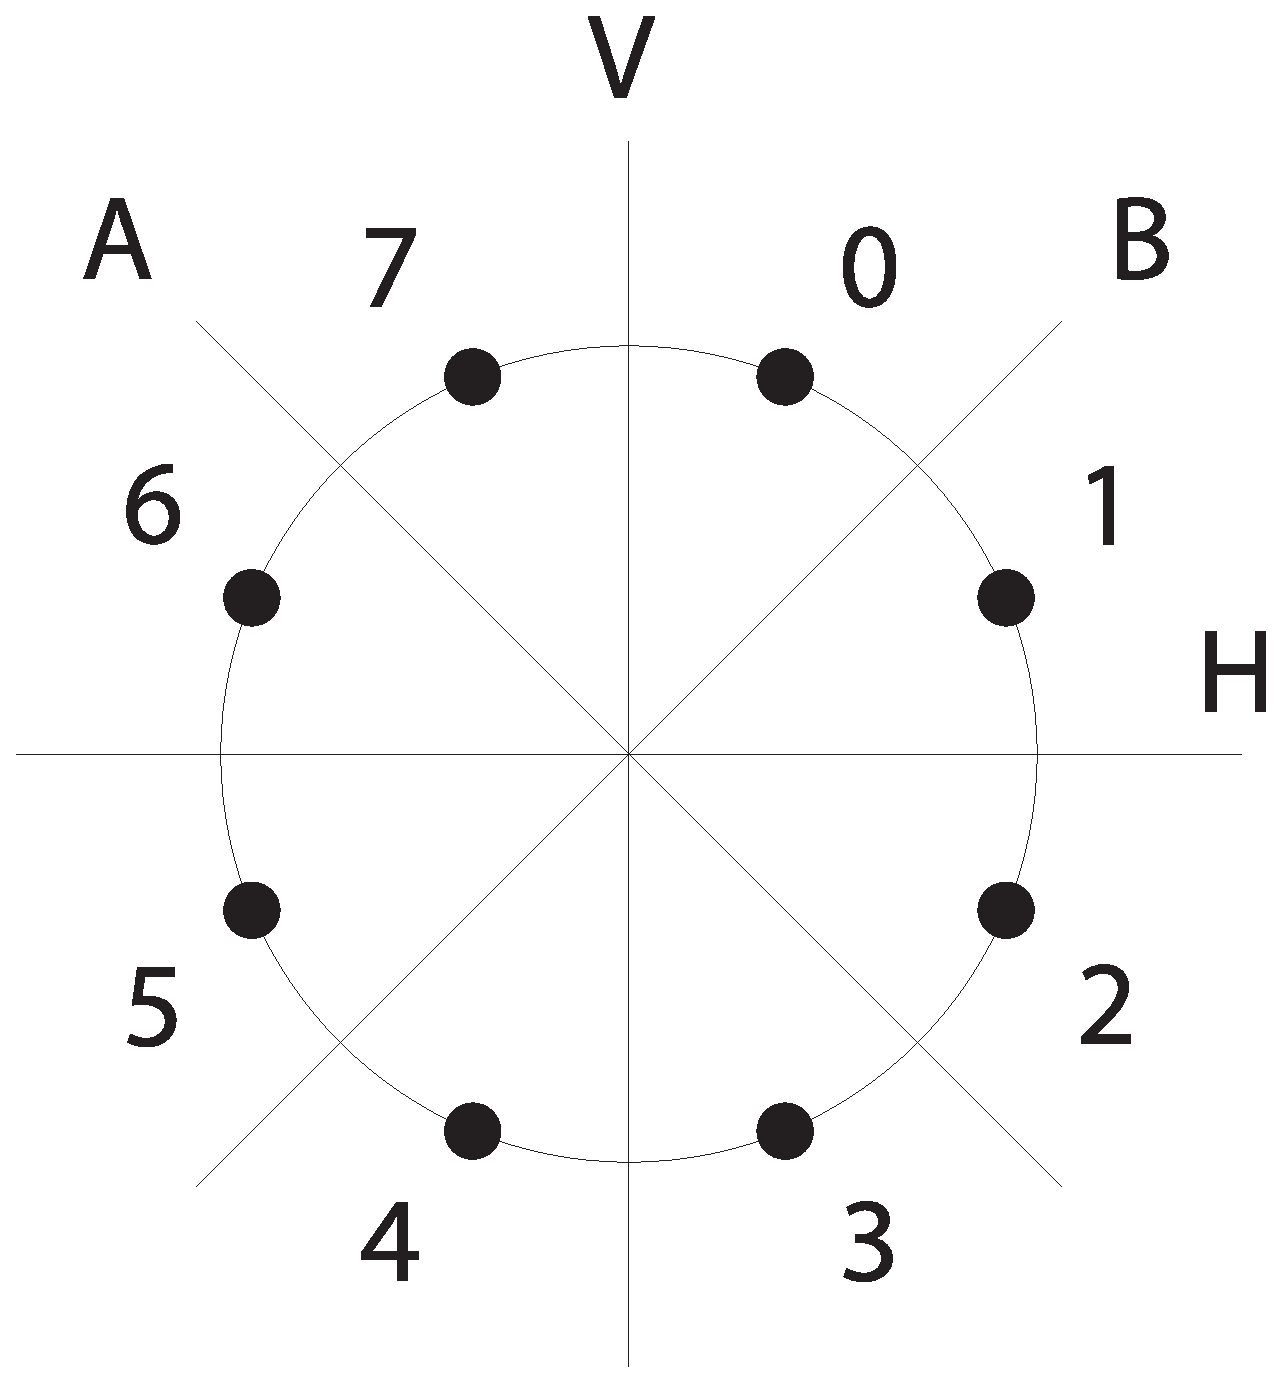
\includegraphics[width=0.4\textwidth]{Fig1}
   %\caption{{\bf Possible sequence positions and reflection axes.} $\Sigma$ points around a circle to map current position in the octagon, and the reflection axes.}\label{fig:circle}
   \caption{{\bf Posibles posiciones de la secuencia y ejes de reflexión} $\Sigma$ apunta alrededor de un círculo para mapear la posición actual en el octágono y los ejes de reflexión}\label{fig:circle}
\end{figure}

%The production rules of grammar $\geom$ were selected based on previous claims of the universality of certain human geometrical knowledge  \cite{izard2011geometry,dehaene2006core,dillon2013core} such as spatial notions \cite{landau1981spatial,lee2012navigation} and detection of symmetries \cite{westphal2012production,machilsen2009role}.

Las reglas de producción de la gramática $\geom$ fueron seleccionadas en base a afirmaciones previa de la universalidad de cierto conocimiento geométrico humano \cite{izard2011geometry,dehaene2006core,dillon2013core} como nociones espaciales \cite{landau1981spatial,lee2012navigation} y detección de geometrías \cite{westphal2012production,machilsen2009role}.

%With these production rules, sequences are described by concatenating or repeating sequence of movements in the octagon. The original set of productions is shown in Table~\ref{table:originalgrammar} and --besides the concatenation and repetition operators-- it includes the following family of atomic geometrical transition productions: anticlockwise movements, staying at the same location, clockwise movements and symmetry movements.

Con estas reglas de producción, las secuencias se describen concatenando o repitiendo secuencias de movimientos en el octágono. El conjunto original de producciones se muestra en la Tabla~\ref{table:originalgrammar} y --además de los operadores de concatenación y repetición-- incluye la siguiente familia de producciones atómicas de transición geométrica: movimientos en sentido antihorario, permanecer en la misma ubicación, movimientos en sentido horario y movimientos de simetría.

\begin{table}[!ht]
\centering
\caption{{\bf Gramática original}}
\label{table:originalgrammar}
\resizebox{\columnwidth}{!}{%
\begin{tabular}{lll|l}
\\{\bf Producción inicial} \\
\thickhline
START & $\rightarrow$ & [INST] & símbolo inicial \\
\hline
\\ {\bf Producciones básicas} \\
\thickhline
INST  & $\rightarrow$ & ATOMIC & producción atómica \\
INST  & $\rightarrow$ & INST,INST & concatenación \\
INST  & $\rightarrow$ & $\text{REP[INST]}^n$ & familia repetir con $n \in [2,8]$ \\

REP  & $\rightarrow$ & REP0 & repetición simple \\

REP  & $\rightarrow$ & REP1$<$ATOMIC$>$ & repetir con variación del punto de inicio usando ATOMIC\\

REP  & $\rightarrow$ & REP2$<$ATOMIC$>$ & repetir con variación de la secuencia resultante usando ATOMIC\\
\hline
\\ {\bf Atomic productions} \\
\thickhline
ATOMIC  & $\rightarrow$ & -1 & siguiente elemento en sentido antihorario (ACW) \\
ATOMIC  & $\rightarrow$ & -2 & segundo elemento ACW \\
ATOMIC  & $\rightarrow$ & -3 & tercer elemento ACW \\
ATOMIC  & $\rightarrow$ & +0 & permanecer en la misma posición \\
ATOMIC  & $\rightarrow$ & +1 & siguiente elemento en sentido horario (CW)\\
ATOMIC  & $\rightarrow$ & +2 & segundo elemento CW \\
ATOMIC  & $\rightarrow$ & +3 & tercer elemento CW \\
ATOMIC  & $\rightarrow$ & A & simetría alrededor de un eje diagonal \\
ATOMIC  & $\rightarrow$ & B & simetría alrededor del otro eje diagonal \\
ATOMIC  & $\rightarrow$ & H & simetría horizontal \\
ATOMIC  & $\rightarrow$ & V & simetría vertical \\
ATOMIC  & $\rightarrow$ & P & simetría rotacional \\
\hline
\end{tabular}}
\end{table}

%The language actually supports not just a simple $n$ times repetition of a block of productions, but it also supports two more complex productions in the repetition family: repeating with a change in the starting point after each cycle and repeating with a change to the resulting sequence after each cycle. More details about the formal syntax and semantics can be found in \cite{marie2016}, though they are not needed here.

El lenguaje en realidad admite no sólo una simple repetición $n$ veces de un bloque de producciones, también admite dos producciones más complejas en la familia de repeticiones: repitiendo con un cambio en el punto de inicio después de cada ciclo y repitiendo con un cambio en la secuencia resultante después de cada ciclo. Más detalles sobre la sintaxis formal y la semántica se pueden encontrar en \cite{marie2016}, aunque no son necesarios aquí. 

%Each program $p$ generated by the grammar describes a mapping $\Sigma\to\Sigma^+$, for $\Sigma=\{0,\dots,7\}$. Here, $\Sigma^+$ represents the set of all (non empty) finite sequences over the alphabet $\Sigma$, which can be understood as a finite sequence of points in the octagon. These programs must then be executed or interpreted from a starting point in order to get the resulting sequence of points. Let $p = \textrm{[+1,+1]}$ be a program, then $p(0)$ is the result of executing $p$ starting from point $0$ (that is, sequence $1,2$) and $p(4)$ is the result of executing the same program starting from point $4$ in the octagon (sequence $5,6$).

Cada programa $p$ generado por la gramática describe un mapeo $\Sigma\to\Sigma^+$, para $\Sigma=\{0,\dots,7\}$. Aquí, $\Sigma^+$ representa el conjunto de todas las secuencias finitas (no vacías) sobre el alfabeto $\Sigma$, que puede entenderse como una secuencia finita de puntos en el octágono. Estos programas luego deben ejecutarse o interpretarse desde un punto de partida para obtener como resultado la secuencia de puntos. Sea $p = \textrm{[+1,+1]}$ un programa, entonces $p(0)$ es el resultado de ejecutar $p$ a partir del punto $0$ (es decir, la secuencia $1,2$) y $p(4)$ es el resultado de ejecutar el mismo programa a partir del punto $4$ del octágono (es decir, la secuencia $5,6$).

%Each sequence can be described with many different programs: from a simple concatenation of atomic productions to more compressed forms using repetitions. For example, to move through all the octagon clockwise one point at a time starting from point $0$, one can use $\textrm{[+1,+1,+1,+1,+1,+1,+1,+1]}(0)$ or $\textrm{[REP[+1]}^8](0)$ or $\textrm{[REP[+1]}^7,\textrm{+1]}(0)$, etc. To alternate $8$ times between points $6$ and $7$, one can use a reflection production like $\textrm{[REP[A]}^8](6)$, or $\textrm{[REP[+1,-1]}^4](6)$.

Cada secuencia se puede describir con muchos programas diferentes: desde una simple concatenación de producciones atómicas a formas más comprimidas utilizando repeticiones. Por ejemplo, para moverse a través de todo el octágono en el sentido de las agujas del reloj, un punto a la vez comenzando desde el punto $0$, uno puede utilizar $\textrm{[+1,+1,+1,+1,+1,+1,+1,+1]}(0)$ o $\textrm{[REP[+1]}^8](0)$ o $\textrm{[REP[+1]}^7,\textrm{+1]}(0)$, etc. Para alternar $8$ veces entre los puntos $6$ y $7$, uno puede utilizar una producción de reflexión como $\textrm{[REP[A]}^8](6)$, o $\textrm{[REP[+1,-1]}^4](6)$.

%\subsection{$\geom$'s original experiment}
\subsection{Experimento original de $\geom$}

%To infer the productions from the observed data, we used the original data from the experiment in \cite{marie2016}. In the experiment, volunteers were exposed to a series of spatial sequences defined on an octagon and were asked to predict future locations. The sequences were selected according to their MDL in the \textit{language of geometry} so that each sequence could be easily described with few productions.

Para inferir las producciones a partir de los datos observados, utilizamos los datos originales del experimento en \cite{marie2016}. En el experimento, los voluntarios fueron expuestos a una serie de secuencias espaciales definidas en un octágono y se les pidió que pronosticaran ubicaciones futuras. Las secuencias se seleccionaron de acuerdo con su MDL en el \textit{lenguaje de geometría} para que cada secuencia pueda ser descripta fácilmente con pocas producciones.

%\paragraph{Participants} The data used in this work comes, except otherwise stated, from Experiment 1 in which participants were 23 French adults (12 female, mean age $= 26.6$, age range $= 20 - 46$) with college-level education. Data from Experiment 2 is later used when comparing adults and children results. In the later, participants where 24 preschoolers (minimal age $= 5.33$, max $= 6.29$, mean $= 5.83 \pm 0.05$).

\paragraph{Participantes:} Los datos utilizados en este trabajo provienen, salvo que se indique lo contrario, del Experimento 1 en el que los participantes eran 23 adultos franceses (12 mujeres, edad media $= 26.6$, rango de edad $= 20 - 46$) con educación de nivel universitario. Los datos del Experimento 2 se utilizan más adelante cuando se comparan los resultados de adultos y niños. En el último, los participantes fueron 24 niños en edad preescolar (edad mínima $= 5.33$, edad máxima $= 6.29$, media $= 5.83 \pm 0.05$).

%\paragraph{Procedure} On each trial, the first two points from the sequence were flashed sequentially in the octagon and the user had to click on the next location. If the subject selected the correct location, she was asked to continue with the next point until the eight points of the sequences were completed. If there was an error at any point, the mistake was corrected, the sequence flashed again from the first point to the corrected point and the user asked to predict the next location. Each $d_i \in \Sigma^8$ from our dataset $D$ is thus the sequence of eight positions clicked in each subject's trial. The detailed procedure can be found in the cited work.

\paragraph{Procedimiento:} En cada prueba, los dos primeros puntos de la secuencia se muestran con un destello de manera secuencial en el octágono y el usuario tiene que hacer clic luego en la siguiente ubicación. Si el sujeto selecciona la ubicación correcta, se le pide que continúe con el siguiente punto hasta que los ocho puntos de la secuencia se completan. Si hubo un error en algún momento, se corrige el error, la secuencia vuelve a mostrarse desde el primer punto hasta el punto corregido y se le solicita al usuario predecir la siguiente ubicación. Cada $d_i \in \Sigma^8$ de nuestro conjunto de datos $D$ es, por tanto, la secuencia de las ocho posiciones que hizo clic en cada prueba cada sujeto. El procedimiento detallado se puede encontrar en el citado trabajo.

%\subsection{Extending $\geom$'s grammar}
\subsection{Extendiendo la gramática de $\geom$}

%We will now expand the original set of productions in $\geom$ with a new set of productions that can also express regularities but are not related to any geometrical intuitions to test our Bayesian inference model.

Ahora ampliaremos el conjunto original de producciones en $\geom$ con un nuevo conjunto de producciones que también pueden expresar regularidades pero que no están relacionadas con ninguna intuición geométrica para probar nuestro modelo de inferencia Bayesiano.

%In Table~\ref{table:adhoc} we show the new set of productions which includes instructions like moving to the point whose label is the square of the current location's label, or using the current point location $i$ to select the $i^\text{th}$digit of a well-known number like $\pi$ or Chaitin's number (calculated for a particular universal Turing Machine and programs up to 84 bits long \cite{calude2002computing}). All digits are returned in arithmetic module 8 to get a valid point for the next position. For example, $\textrm{PI}(0)$  returns the first digit of $\pi$, that is $\textrm{PI}(0)= 3 \mod({8}) = 3$; and $\textrm{PI}(1) = 1$.

En la Tabla~\ref{table:adhoc} mostramos el nuevo conjunto de producciones que incluye instrucciones tales como moverse al punto cuya ubicación es el cuadrado de la ubicación actual, o utilizar el punto actual $i$ para seleccionar el $i^\text{th}$dígito de un número conocido como $\pi$ o el número de Chaitín (calculado para una máquina universal de Turing particular y programas de hasta 84 bits \cite{calude2002computing}). Todos los dígitos se devuelven en módulo aritmético 8 para obtener una posición válida. Por ejemplo, $\textrm{PI}(0)$ retorna el primer dígito de $\pi$, es decir $\textrm{PI}(0)= 3 \mod({8}) = 3$; y $\textrm{PI}(1) = 1$.

\begin{table}[!ht]
\centering
\caption{{\bf Producciones ad-hoc}}
\label{table:adhoc}
\begin{tabular}{lll|l}
\thickhline
ATOMIC  & $\rightarrow$ & DOUBLE & $($ubicación $*\ 2) \mod 8$  \\
ATOMIC  & $\rightarrow$ & -DOUBLE & $($ubicación $* -2) \mod 8$ \\
ATOMIC  & $\rightarrow$ & SQUARE & $($ubicación$^2) \mod 8$ \\
ATOMIC  & $\rightarrow$ & GAMMA & $\Gamma($ubicación$+1) \mod 8$ \\
ATOMIC  & $\rightarrow$ & PI & ubicación-ésimo dígito de $\pi$ \\
ATOMIC  & $\rightarrow$ & EULER & ubicación-ésimo dígito de $e$ \\
ATOMIC  & $\rightarrow$ & GOLD & ubicación-ésimo dígito de $\phi$ \\
ATOMIC  & $\rightarrow$ & PYTH & ubicación-ésimo dígito de$\sqrt{2}$ \\
ATOMIC  & $\rightarrow$ & KHINCHIN & ubicación-ésimo dígito de la constante de Khinchin\\
ATOMIC  & $\rightarrow$ & GLAISHER & ubicación-ésimo dígito de la constante de Glaisher\\
ATOMIC  & $\rightarrow$ & CHAITIN & ubicación-ésimo dígito de la constante de Chaitín Omega\\
\hline
\end{tabular}
\end{table}

%\subsection{Inference results for $\geom$}
\subsection{Resultados de inferencia para $\geom$}

%To let the MCMC converge faster (and to later compare the concept's probability with their corresponding MDL), we generated all the programs that explain each of the observed sequences from the experiment. In this way, we are able to sample from the exact distribution $P(p_i \mid d_i, \theta)$ by sampling from a multinomial distribution of all the possible programs $p_i$ that compute $d_i$, where each $p_i$ has probability of occurrence equal to $P(p_i \mid \theta)$.

Para permitir que la MCMC converja más rápido (y luego comparar la probabilidad del concepto con su correspondiente MDL), generamos todos los programas que explican cada una de las secuencias observadas del experimento. De esta manera, podemos tomar muestras de la distribución $P(p_i \mid d_i, \theta)$ por muestreo de una distribución multinomial de todos los posibles programas $p_i$ que computan $d_i$, donde cada $p_i$ tiene una probabilidad de ocurrencia igual a $P(p_i \mid \theta)$.

%To get an idea of the expressiveness of the grammar to generate different programs for a sequence and the cost of computing them, it is worth mentioning that there are more than 159 million programs that compute the 292 unique sequences generated by the subjects in the experiment, and that for each sequence there is an average of 546,713 programs (min = $10,749$, max = $5,500,026$, $\sigma$ = $693,618$).

Para tener una intuición de la expresividad de la gramática para para generar diferentes programas para una secuencia y el costo de calcularlos, vale la pena mencionar que hay más de 159 millones de programas que computan las 292 secuencias únicas generadas por los sujetos en el experimento y que, para cada secuencia, hay un promedio de 546,713 programas (mín = $10,749$, máx = $5,500,026$, $\sigma$ = $693,618$).

%\figref{fig:inferredtheta} shows the inferred $\theta$ for the observed sequences from subjects, with a unit concentration parameter for the Dirichlet prior, $\alpha = (1, \dots, 1)$. Each bar shows the mean probability and the standard error of each of the atomic productions after 50 steps of the MCMC, leaving the first 10 steps out as burn-in.

La \figref{fig:inferredtheta} muestra el $\theta$ inferido para las secuencias observadas de los sujetos, con el hiperparámetro de la Dirichlet inicial en $\alpha = (1, \dots, 1)$. Cada barra muestra la probabilidad media y el error estándar de cada una de las producciones atómicas después de 50 pasos de la MCMC, dejando fuera los primeros 10 pasos como iteraciones de \textit{burn-in}.

\begin{figure}[htpb]
    \centering
    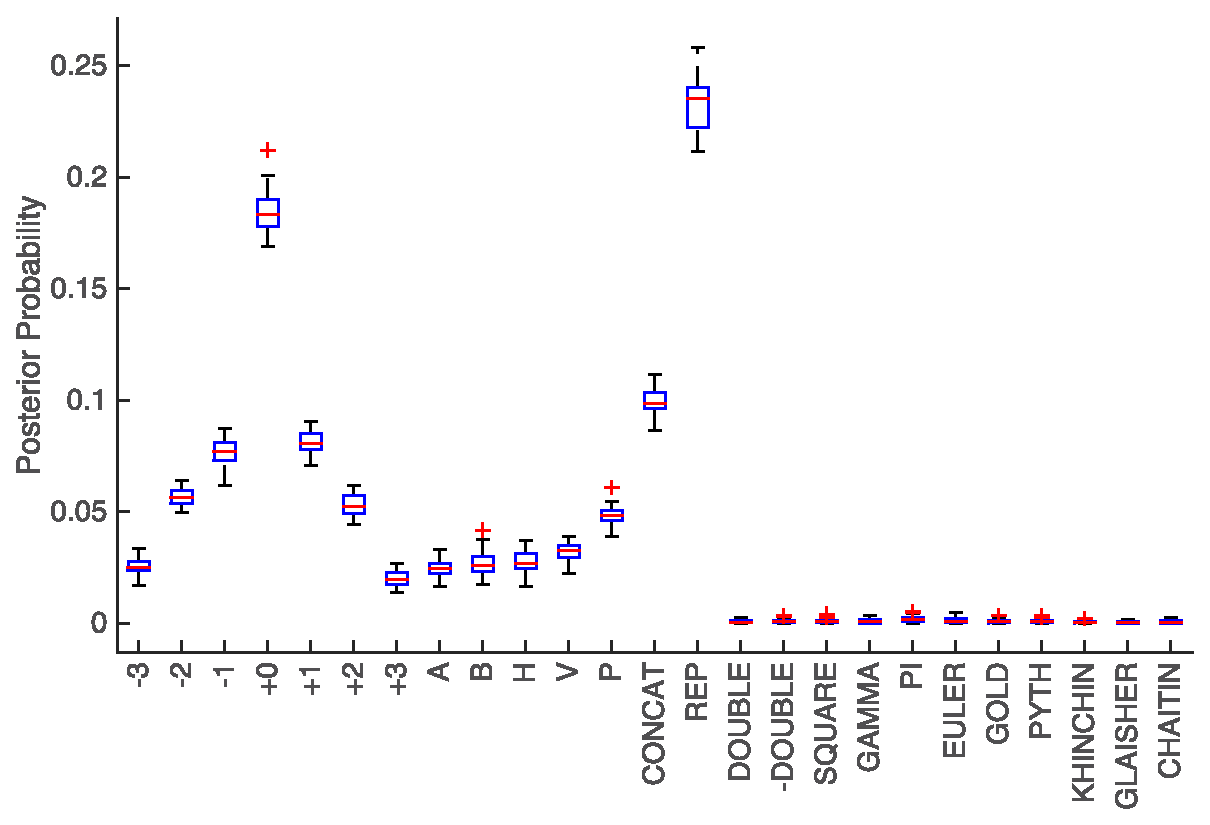
\includegraphics[width=0.4\textwidth]{Fig2}
    %\caption{\bf{Inferred $\theta_i$.} Inferred probability for each production in the grammar}
    \caption{\bf{$\theta_i$ inferido} Probabilidad inferida para cada producción de la gramática}
    \label{fig:inferredtheta}
\end{figure}

Aunque 50 pasos puedan parecer bajos para que converja un algoritmo de MCMC, nuestro método calculó $P(p_i \mid d_i, \theta)$ de manera exacta para acelerar la convergencia y para poder luego comparar la probabilidad con la complejidad del modelo MDL original. En la \figref{fig:convergetheta}, mostramos una traza de ejemplo para cuatro ejecuciones de MCMC para $\theta_{\text{+0}}$, que corresponde al valor atómico de la producción +0, pero es representativo del comportamiento de todos los $\theta_i$. (consulte los \nameref{S1_Fig} para las trazas del conjunto entero de producciones).

\begin{figure}[htpb]
    \centering
    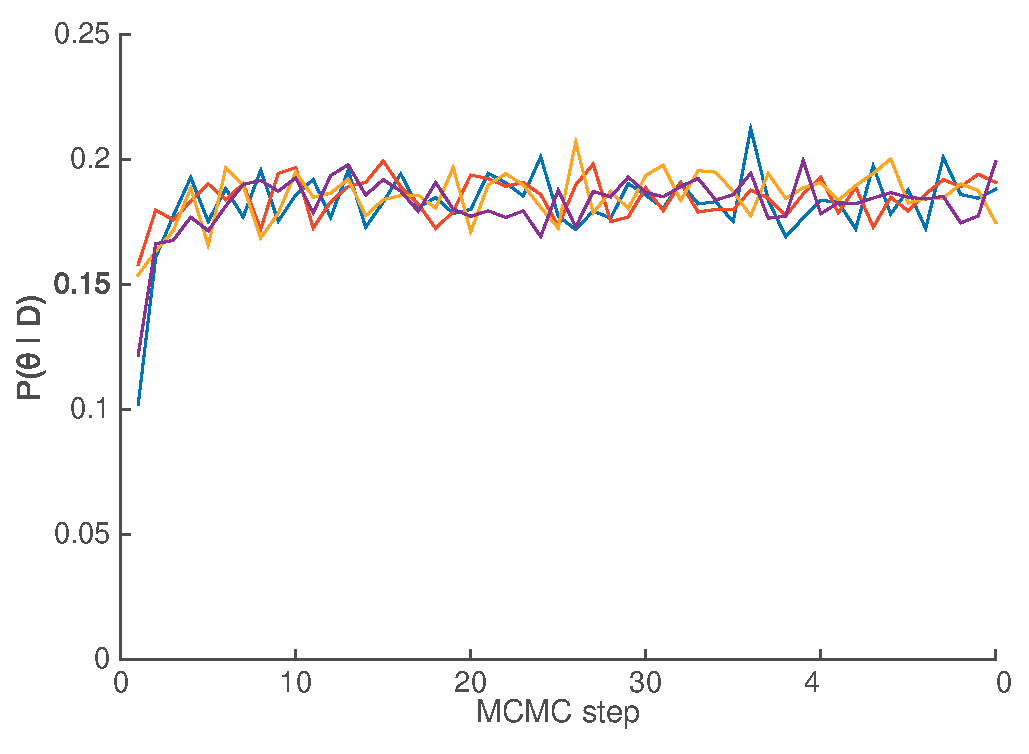
\includegraphics[width=0.4\textwidth]{Fig3}
    %\caption{{\bf Inferred $\theta_{\text{+0}}$.} Inferred probability for +0 production at each step in four MCMC chains.}
    \caption{{\bf $\theta_{\text{+0}}$ inferido.} Probabilidad inferida para +0 en cada paso para cuatro cadenas de MCMC.}
    \label{fig:convergetheta}
\end{figure}

%\figref{fig:inferredtheta} shows a remarkable difference between the probability of the productions that were originally used based on geometrical intuitions and the ad-hoc productions. The plot also shows that each clockwise production has almost the same probability as its corresponding anticlockwise production, and a similar relation appears between horizontal and vertical symmetry (H and V) and symmetries around diagonal axes (A and B). This is important because the original experiment was designed to balance such behavior; the inferred grammar reflects this.

La \figref{fig:inferredtheta} muestra una diferencia notable entre la probabilidad de las producciones que se utilizaron originalmente sobre la base de intuiciones geométricas y las producciones ad-hoc. El gráfico muestra también que cada producción en el sentido horario tiene casi la misma probabilidad que su correspondiente producción en sentido antihorario, y una relación similar aparece entre la simetría horizontal y la vertical (H y V) y las simetrías alrededor de los ejes diagonales (A y B). Esto es importante porque el experimento original fue diseñado para equilibrar tal comportamiento y la gramática inferida lo refleja también.

%\figref{fig:thetaGrouped} shows the same inferred $\theta$ but grouped according to production family. Grouping stresses the low probability of all the ad-hoc productions, but also shows an important difference between REP and the rest of the productions, particularly the simple concatenation of productions (CONCAT). This indicates that the \textit{language of geometry} is capable of reusing simpler structures that capture geometrical meaning to explain the observed data, a key aspect of a successful model of LoT.

La \figref{fig:thetaGrouped} muestra el mismo $\theta$ inferido pero agrupado según su familia de producción. El agrupamiento destaca la baja probabilidad de todas las producciones ad-hoc, pero también muestra una diferencia importante entre REP y el resto de las producciones, particularmente respecto de la simple concatenación de producción (CONCAT). Esto indica que el lenguaje de geometría es capaz de reutilizar estructuras más simples que captura el significado geométrico para explicar los datos observados, un aspecto clave de un modelo exitoso de LoT que también se ve reflejado en la gramática inferida.

\begin{figure}[!ht]
    \centering
    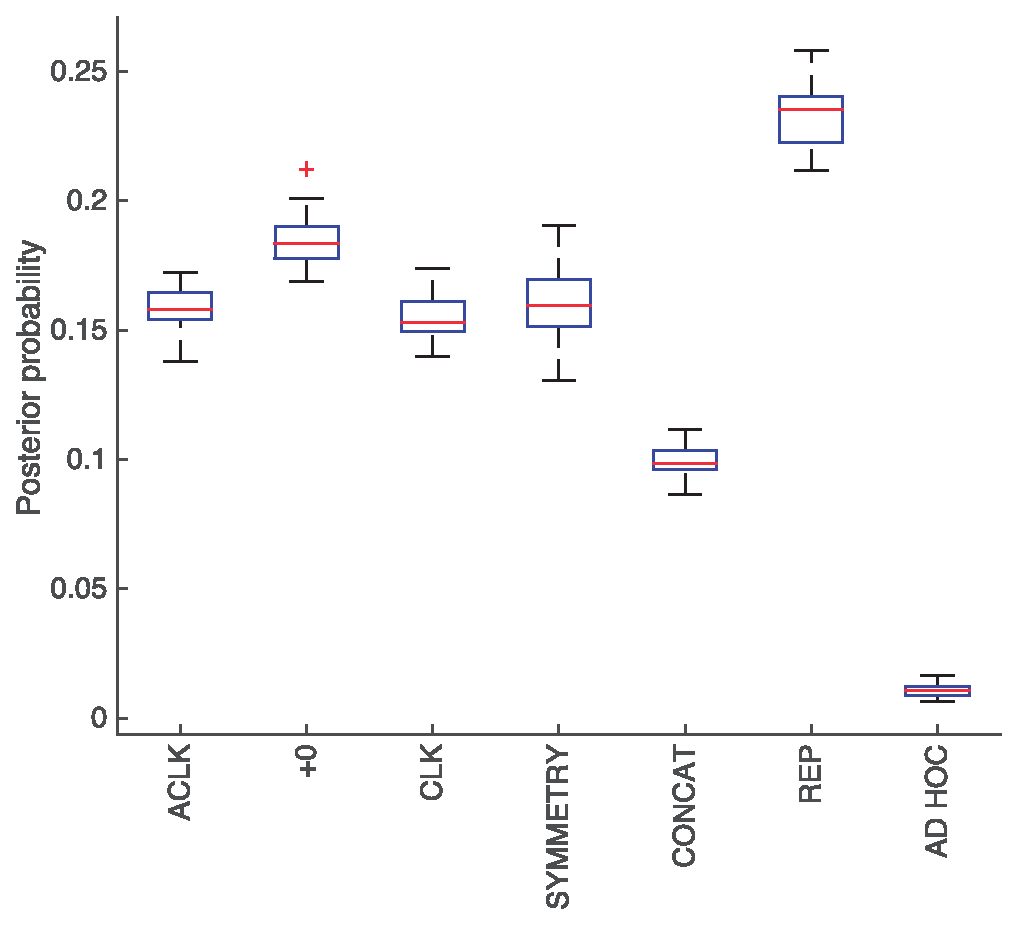
\includegraphics[width=0.4\textwidth]{Fig4}
    \caption{{\bf $\theta_i$ inferido agrupado por familia.} Probabilidad inferida para cada producción en la gramática, agrupada por familia.}
    \label{fig:thetaGrouped}
\end{figure}

%We then ran the same inference method using observed sequences from other experiments but only with the original grammar productions (i.e.\ setting aside the ad-hoc productions). We compared the result of inferring over our previously analyzed sequences generated by adults with sequences generated by children (experiment 2 from  \cite{marie2016}) and the actual expected sequences for an ideal player.

Luego ejecutamos el mismo método de inferencia utilizando las secuencia observadas en otros experimentos, pero sólo con las producciones gramaticales originales (es decir, dejando de lado las producciones ad-hoc). Comparamos el resultado de inferir sobre nuestras secuencias previamente analizadas (que habían sido generadas por adultos) con aquellas generadas por niños (el Experimento 2 de   \cite{marie2016}) y con las secuencias esperadas para un jugador ideal.

%\figref{fig:adultVsChildren} shows the probabilities for each atomic production that is inferred after each population. The figure denotes that different populations can converge to different probabilities and thus different LoTs. Specifically, it is worth mentioning that the ideal learner indeed uses more repetition productions than simple concatenations when compared to adults. In the same way, adults use more repetitions than children. This could mean that the ideal learner is capable of reproducing the sequences by recursively embedding other smaller programs, whereas adults and children more so have problems understanding or learning the smaller concept that can explain all the sequences from the experiments, which is consistent with the results from the MDL model in \cite{marie2016}.

La \figref{fig:adultVsChildren} muestra las probabilidades para cada producción atómica que se infieren de los datos de cada población. La figura denota que diferentes poblaciones pueden converger a diferentes probabilidades y, por tanto, a diferentes LoT. Específicamente, vale la pena mencionar que el sujeto ideal de hecho utiliza más producciones de repetición que simples concatenaciones en comparación con los adultos. Del mismo modo, los adultos utilizan más repeticiones que los niños. Esto podría significar que el sujeto ideal es capaz de reproducir las secuencias reutilizando de manera recursiva otros programas más pequeños, mientras que los adultos y los niños tienen más problemas para comprender o aprender el programa más pequeño que puede explicar cada una de las secuencias de los experimentos, lo cuál es consistente con los resultados del modelo de MDL en \cite{marie2016}.

\begin{figure}[!ht]
    \centering
    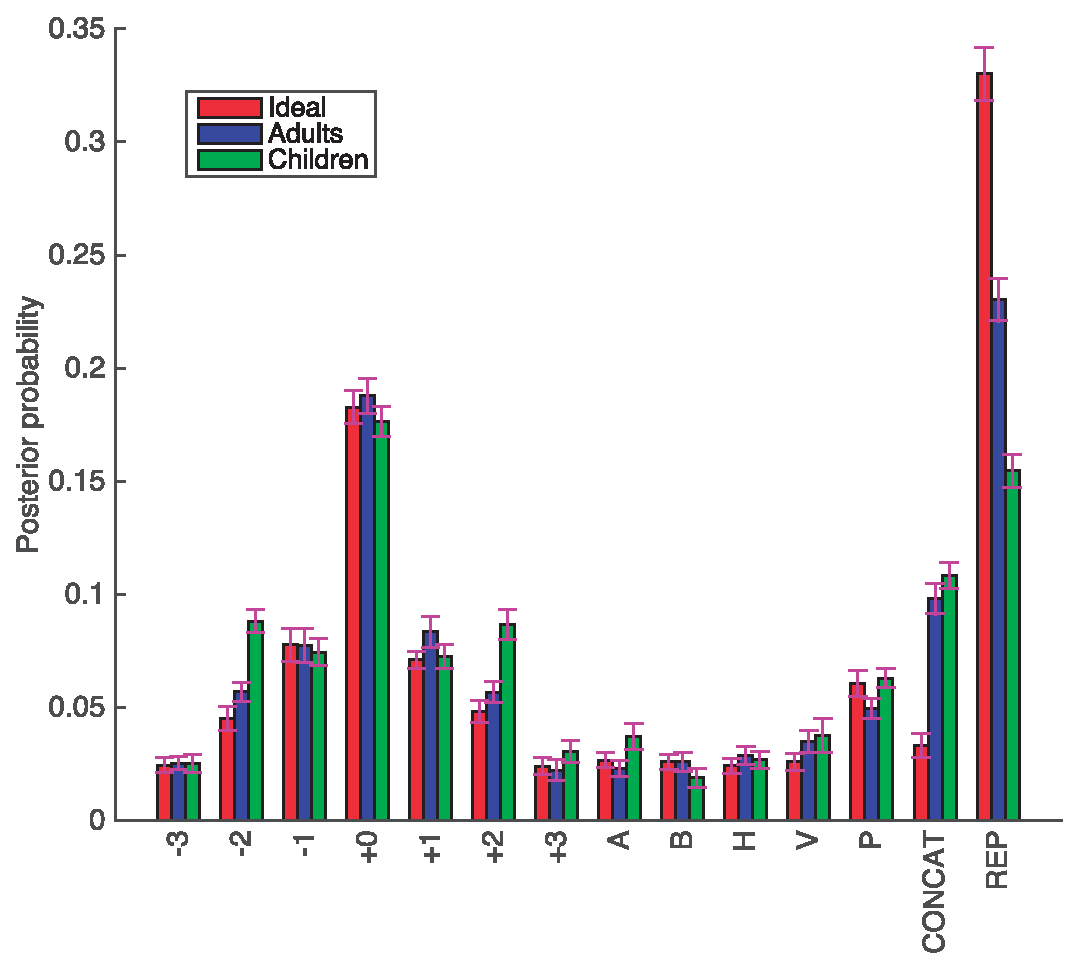
\includegraphics[width=0.4\textwidth]{Fig5}
    %\caption{{\bf Inferred $\theta_i$ for ideal learner, adults and children.} Inferred probability for each production in the grammar for different population data.}
    \caption{{\bf $\theta_i$ inferido para el sujeto ideal, adultos y niños} Probabilidad inferida para cada producción de la gramática para las diferentes poblaciones.}
    \label{fig:adultVsChildren}
\end{figure}

%It is worth mentioning that in \cite{marie2016} the complete grammar for the \textit{language of geometry} could explain adults' behavior but had problems to reproduce the children's patterns for some sequences. However, they also showed that penalizing the rotational symmetry (P) could adequately explain children's behavior. In \figref{fig:adultVsChildren}, we see that the mean value of (P) for children is 0.06 whereas in adults it's 0.05 (a two-sample t-test reveals t = -12.6, p = 10-19). This might not necessarily be contradictory, as the model for children in \cite{marie2016} was used to predict the next symbol of a sequence after seeing its prefix by adding a penalization for extensions that use the rotational symmetry in the {\em minimal} program of each sequence. On the other hand, the Bayesian model in this work tries to explain the observed sequences produced by children considering the probability of a sequence summing over {\em all} the possible programs that can generate it and not just the ones with minimal size. Thus, a production like (P) that might not be part of the minimal program for a sequence might not necessarily be less probable when considering the entire distribution of programs for that same sequence.

Cabe mencionar que en \cite{marie2016} la gramática completa para el \textit{lenguaje de geometría} podía explicar el comportamiento de los adultos, pero tenía problemas para reproducir los patrones de los niños para algunas secuencias. Sin embargo, también demostraron que penalizar a la simetría rotacional (P) podría explicar adecuadamente el comportamiento de los niños. En la \figref{fig:adultVsChildren}, vemos que el valor medio de (P) para niños es 0.06 mientras que en adultos es 0.05 (una prueba-t de dos muestras revela que t = -12.6, p = 10-19). Esto puede no ser necesariamente contradictorio, ya que el modelo para niños en \cite{marie2016} se utilizó para predecir el siguiente símbolo de una secuencia después de ver su prefijo agregando una penalización para extensiones que usan la simetría rotacional (P) \textit{en el programa mínimo} de cada secuencia. Por otro lado, el modelo Bayesiano en este trabajo intenta explicar las secuencias observadas producidas por los niños considerando la probabilidad de una secuencia a partir de sumar todos los posibles programas que la pueden generar \textit{y no sólo en los de tamaño mínimo}. Así, una producción como (P) que podría no ser parte del programa mínimo para una secuencia, puede no ser necesariamente menos probable cuando se considera la distribución total de programas para esa misma secuencia.

%\section{Coding Theorem}
\section{Teorema de codificación}
\label{sec:coding}

%For each phenomenon there can always be an extremely large, possibly infinite, number of explanations. In a LoT model, this space is constrained by the grammar $\gram$ that defines the valid hypotheses in the language. Still, one has to define how a hypothesis is chosen among all possibilities. Following Occam's razor, one should choose the simplest hypothesis amongst all the possible ones that explain a phenomenon. In cognitive science, the MDL framework has been widely used to model such bias in human cognition, and in \textit{the language of geometry} in particular \cite{marie2016}. The MDL framework is based on the ideas of information theory \cite{shannon48}, Kolmogorov complexity \cite{kolmogorov1968three} and Solomonoff induction \cite{solomonoff1964formal}.

Para cada fenómeno siempre puede haber un número extremadamente grande, posiblemente infinito, de explicaciones. En un modelo de LoT, este espacio está limitado por la gramática $\gram$ que define las hipótesis válidas en el lenguaje. Aún así, hay que definir cómo se elige una hipótesis entre todas las posibles. Siguiendo el principio de la navaja de Ockham, se debe elegir la hipótesis más simple entre todas las posibles que explican un fenómeno. En ciencia cognitiva, y en el lenguaje de geometría en particular, la MDL se suele utilizar para modelar tal sesgo en la cognición humana. La MDL se basa sobre las ideas de la teoría de la información \cite{shannon48}, la complejidad de Kolmogorov \cite{kolmogorov1968three} y la inducción de Solomonoff \cite{solomonoff1964formal}.

%Occam's razor was formalized by Solomonoff \cite{solomonoff1964formal} in his theory of universal inductive inference, which proposes a universal prediction method that successfully approximates any distribution $\mu$ based on previous observations, with the only assumption of $\mu$ being computable. In short, Solomonoff's theory uses all programs (in the form of prefix Turing machines) that can describe previous observations of a sequence to calculate the probability of the next symbols in an optimal fashion, giving more weight to shorter programs. Intuitively, simpler theories with low complexity have higher probability than theories with higher complexity. Formally, this relationship is described by the Coding Theorem \cite{levin1974laws}, which closes the gap between the concepts of Kolmogorov complexity and probability theory. However, LoT models that define a probabilistic distribution for their hypotheses do not attempt to compare it with a complexity measure of the hypotheses like the ones used in MDL, nor the other way around.

El principio de la navaja de Ockham fue formalizado por Solomonoff \cite{solomonoff1964formal} en su teoría universal de la inferencia inductiva, que propone un método de predicción universal que aproxima cualquier distribución $\mu$ a partir de observaciones previas, con el único supuesto de que $\mu$ sea computable. En resumen, la teoría de Solomonoff utiliza todos los programas (en la forma de máquinas de Turing libre de prefijos)
que pueden describir las observaciones previas de una secuencia para calcular la probabilidad de los siguientes símbolos de una manera óptima, dando más peso a los programas más cortos. Intuitivamente, las teorías más simples, con baja complejidad, tienen mayor probabilidad que las teorías de mayor complejidad. Formalmente, esta relación es descrita en el Teorema de codificación \cite{levin1974laws},  que cierra la brecha entre los conceptos de complejidad de Kolmogorov y la teoría de probabilidad. Sin embargo, los modelos de LoT que definen una distribución probabilística para sus hipótesis no han intentado compararla con una medida de complejidad de las hipótesis como las que se usan en MDL, ni al revés.

%In what follows we formalize the Coding Theorem (for more information, see \cite{li2013introduction}) and test it experimentally. To the best our knowledge, this is the first attempt to validate these ideas for a particular (non universal) language. The reader should note that we are not validating the theorem itself as it has already been proved for universal Turing Machines. Here, we are testing whether the inverse logarithmic relationship between the probability and complexity holds true when defined for a specific non universal language.

A continuación, formalizamos el Teorema de Codificación (para obtener más información, consulte \cite{li2013introduction}) y lo probamos experimentalmente. Hasta donde sabemos, este es el primer intento para validad estas ideas para un lenguaje particular (no universal). El lector debe tener en cuenta que no estamos validando el teorema en sí, dado que ya ha sido probado para Máquinas de Turing universales. Aquí estamos probando si la relación logarítmica inversa entre la probabilidad y la complejidad podría mantenerse cuando se definen para un lenguaje específico no universal.

%\subsection{The formal statement}
\subsection{La definición formal}

%Let $M$ be a prefix Turing machine --by {\em prefix} we mean that if $M(x)$ is defined, then $M$ is undefined for every proper extension of $x$. Let $P_M(x)$ be the probability that the machine $M$ computes output $x$ when the input is filled-up with the results of fair coin tosses, and let $K_M(x)$ be the {\em Kolmogorov complexity of $x$ relative to $M$}, which is defined as the length of the shortest program which outputs $x$, when executed on $M$. The Coding Theorem states that for every string $x$ we have

Sea $M$ una Máquina de Turing libre de prefijos --por {\em prefijo} nos referimos a que si $M(x)$ está definida, entonces $M$ está indefinida para cualquier extensión de $x$. Sea $P_M(x)$ la probabilidad de que la máquina $M$ compute la salida $x$ cuando la entrada se llena con los resultados de los lanzamientos de una moneda justa, y sea $K_M(x)$ la {\em complejidad de Kolmogorov de $x$ relativa a $M$}, que se define como la longitud del programa más corto que genera $x$, cuando se ejecuta en $M$. El Teorema de Codificación establece que, por cada cadena $x$ tenemos:
%
\begin{equation}
\label{eqF}
\log \frac{1}{P_U(x)} = K_U(x)
\end{equation}
%
%up to an additive constant, whenever $U$ is a {\em universal} prefix Turing machine --by {\em universal} we mean a machine which is capable of simulating every other Turing machine; it can be understood as the underlying (Turing-complete) chosen programming language. It is important to remark that neither $P_U$, nor $K_U$ are computable, which means that such mappings cannot be obtained through effective means. However, for specific (non-universal) machines $M$, one can, indeed, compute both $P_M$ and $K_M$.
hasta una constante aditiva, siempre que $U$ sea una Máquina Universal de Turing de libre prefijos --por {\em Universal} nos referimos a una máquina que es capaz de simular cualquier otra máquina de Turing; puede entenderse como el lenguaje de programación elegido subyacente (Turing-completo)--. Es importante señalar que ni $P_U$, ni $K_U$ son computables, lo que significa que tal mapeo no puede obtenerse por medios efectivos. Sin embargo, para máquinas específicas (no universales) $M$, uno puede --de hecho-- calcular tanto $P_M$ como $K_M$.

%\subsection{Testing the Coding Theorem for \boldmath{$\geom$}}
\subsection{Probando el teorema de codificación para \boldmath{$\geom$}}

%Despite the fact that $P_M$ and $K_M$ are defined over a Turing Machine $M$, the reader should note that a LoT is not usually formalized with a Turing Machine, but instead as a programming language with its own syntax of valid programs and semantics of execution, which stipulates how to compute a concept from a program. However, one can understand programming languages as defining an equivalent (not necessarily universal) Turing Machine model, and a LoT as defining its equivalent (not necessarily universal) Turing Machine $\gram$. In short, machines and languages are interchangeable in this context: they both specify the programs/terms, which are symbolic objects that, in turn, describe semantic objects, namely, strings.

A pesar de que $P_M$ y $K_M$ están definidas sobre una máquina de Turing $M$, el lector debe tener en cuenta que un LoT no se suele formalizar con una máquina de Turing, sino como un lenguaje de programación con su propia sintaxis de programas válidos y su propia semántica de ejecución que estipula cómo calcular un concepto a partir de un programa válido. Sin embargo, uno puede entender los lenguajes de programación como la definición de una máquina de Turing equivalente (no necesariamente universal), y a un LoT como un lenguaje que define a su equivalente máquina de Turing $\gram$ (no necesariamente universal), En resumen, las máquinas y los lenguajes son intercambiables en este  sentido: ambas especifican los programas / términos, los cuales son objetos simbólicos que --a su vez-- describen objetos semánticos (a saber, cadenas). 

%\paragraph{The Kolmogorov complexity relative to \boldmath{$\geom$}}

\paragraph{La complejidad de Kolmogorov relativa a \boldmath{$\geom$}:}
%In \cite{marie2016}, the Minimal Description Length was used to model the combination of productions from the \textit{language of geometry} into concepts by defining a Kolmogorov complexity relative to the {\em language of geometry}, which we denote $K_{\geom}$. $K_{\geom}(x)$ is the minimal size of an expression in the grammar of $\geom$ which describes $x$. The formal definition of `size' can be found in the cited work but in short: each of the atomic productions adds a fixed cost of $2$ units; using any of the repetition productions to iterate $n$ times a list of other productions adds the cost of the list, plus $\lfloor \log(n) \rfloor$; and joining two lists with a concatenation costs the same as the sum of the costs of both lists.

En \cite{marie2016}, la longitud mínima de descripción (MDL) se utilizó para modelar la combinación de las producciones del \textit{lenguaje de geometría} en conceptos mediante la definición de una complejidad de Kolmogorov relativa al {\em lenguaje de geometría}, la cual denotamos como $K_{\geom}$. $K_{\geom}(x)$ es el tamaño mínimo de una expresión en la gramática de $\geom$ que describe $x$. La definición formal de `tamaño' se puede encontrar en el trabajo citado, pero en resumen: cada una de las producciones atómicas agrega un costo fijo de $2$ unidades; utilizando cualquiera de las producciones de repetición para iterar $n$ veces una lista de otras producciones agrega el costo de esta lista más $\lfloor \log(n) \rfloor$; y unir dos listas con una concatenación cuesta lo mismo que la suma de los costos de ambas listas.

%\paragraph{The probability relative to \boldmath{$\geom$}} On the other hand, with the Bayesian model specified in this work, we can define $P(x \mid \geom, \theta)$ which is the probability of a string $x$ relative to $\geom$ and its vector of probabilities for each of the productions.

\paragraph{La probabilidad relativa \boldmath{$\geom$}:} Por otro lado, con el modelo Bayesiano especificado en este trabajo, podemos definir $P(x \mid \geom, \theta)$ que es la probabilidad de una cadena $x$ relativa a $\geom$ y el vector de probabilidades para cada una de las producciones.

%For the sake of simplicity, we will use $P_{\geom}(x)$ to denote $P(x \mid \geom, \theta)$ when $\theta$ is the inferred probability from the observed adult sequences from the experiment.
En aras de la simplicidad, usaremos $P_{\geom}(x)$ para denotar $P(x \mid \geom, \theta)$ cuando $\theta$ es la probabilidad inferida de las secuencias de adultos observadas en el experimento.
%
\begin{eqnarray}
\label{eqG}
P_{\geom}(x) &=& P(x \mid \geom, \theta)\\
&=& \sum_{\prog} P(x \mid \prog, \theta)\\
&\propto &\sum_{prog} P(x \mid \prog) P(\prog \mid \theta).
\end{eqnarray}
%

%Here, we calculate both $P_{\geom}(x)$ and $K_{\geom(x)}$ in an exact way (note that $\geom$, seen as a programming language, is not Turing-complete). In this section, we show an experimental equivalence between such measures which is consistent with the Coding Theorem. We should stress, once more, that the theorem does not predict that this relationship should hold for a specific non-universal Turing Machine.

Aquí, calculamos tanto $P_{\geom}(x)$ como $K_{\geom(x)}$ de una manera exacta (tenga en cuenta que $\geom$, visto como un lenguaje de programación, no es Turing-completo). En esta sección, mostramos un experimento de equivalencia entre tales medidas que es consistente con el Teorema de Codificación. Queremos enfatizar, una vez más, que el teorema no predice que está relación deba mantenerse para una máquina de Turing específica no universal.


%To calculate $P_{\geom}(x)$ we are not interested in the normalization factor of $P(x \mid \prog) P(\prog \mid \theta)$ because we are just trying to measure the relationship between $P_{\geom}$ and $K_{\geom}$ in terms of the Coding Theorem. Note, however, that calculating $P_{\geom}(x)$ involves calculating all programs that compute each of the sequences as in our previous experiment. To make this tractable we calculated $P_{\geom}(x)$ for 10,000 unique random sequences for each of the possible sequence lengths from the experiment (i.e., up to eight). When the length of the sequence did not allow 10,000 unique combinations, we used all the possible sequences of that length.

Para calcular $P_{\geom}(x)$ no nos interesa el factor de normalización de $P(x \mid \prog) P(\prog \mid \theta)$ porque sólo estamos tratando de medir la relación entre $P_{\geom}$ y $K_{\geom}$ en términos del Teorema de Codificación. Sin embargo, tenga en cuenta que el cálculo de $P_{\geom}(x)$ implica calcular todos los programas que computan cada una de las secuencias como en nuestro experimento anterior. Para hacer esto tratable, calculamos $P_{\geom}(x)$ para 10,000 secuencias aleatorias únicas para cada una de las posibles longitudes de las secuencias del experimento (es decir, hasta ocho). Cuando la longitud de la secuencia no permitió 10,000 combinaciones únicas, utilizamos todas las posibles secuencias de esa longitud.

%\subsection{Coding Theorem Results}
\subsection{Resultados del Teorema de Codificación}

%\figref{fig:codR} shows the mean probability $P_{\geom}(x)$ for all sequences $x$ with the same value of $K_{\geom(x)}$ and length between 4 and 8 ($|x| \in \left[4,8 \right]$) for all generated sequences $x$. The data is plotted with a logarithmic scale for the x-axis, illustrating the inverse logarithmic relationship between $K_{\geom}(x)$ and $P_{\geom}(x)$. The fit is very good, with $R^2=.99$, $R^2=.94$, $R^2=.97$, $R^2=.99$ and $R^2=.98$ for \figref{fig:codR}A, \figref{fig:codR}B, \figref{fig:codR}C, \figref{fig:codR}D and \figref{fig:codR}E, respectively.

La \figref{fig:codR} muestra la probabilidad media $P_{\geom}(x)$ para todas las secuencias $x$ con el mismo valor de $K_{\geom(x)}$ y una longitud entre 4 y 8 ($|x| \in \left[4,8 \right]$) para todas las secuencias generadas $x$. Los datos se trazan con una escala logarítmica para el eje x, ilustrando la relación logarítmica inversa entre $K_{\geom}(x)$ y $P_{\geom}(x)$. El ajuste es muy bueno, con $R^2=.99$, $R^2=.94$, $R^2=.97$, $R^2=.99$ y $R^2=.98$ para \figref{fig:codR}A, \figref{fig:codR}B, \figref{fig:codR}C, \figref{fig:codR}D y \figref{fig:codR}E, respectivamente.

\begin{figure}[!ht]
    \centering
    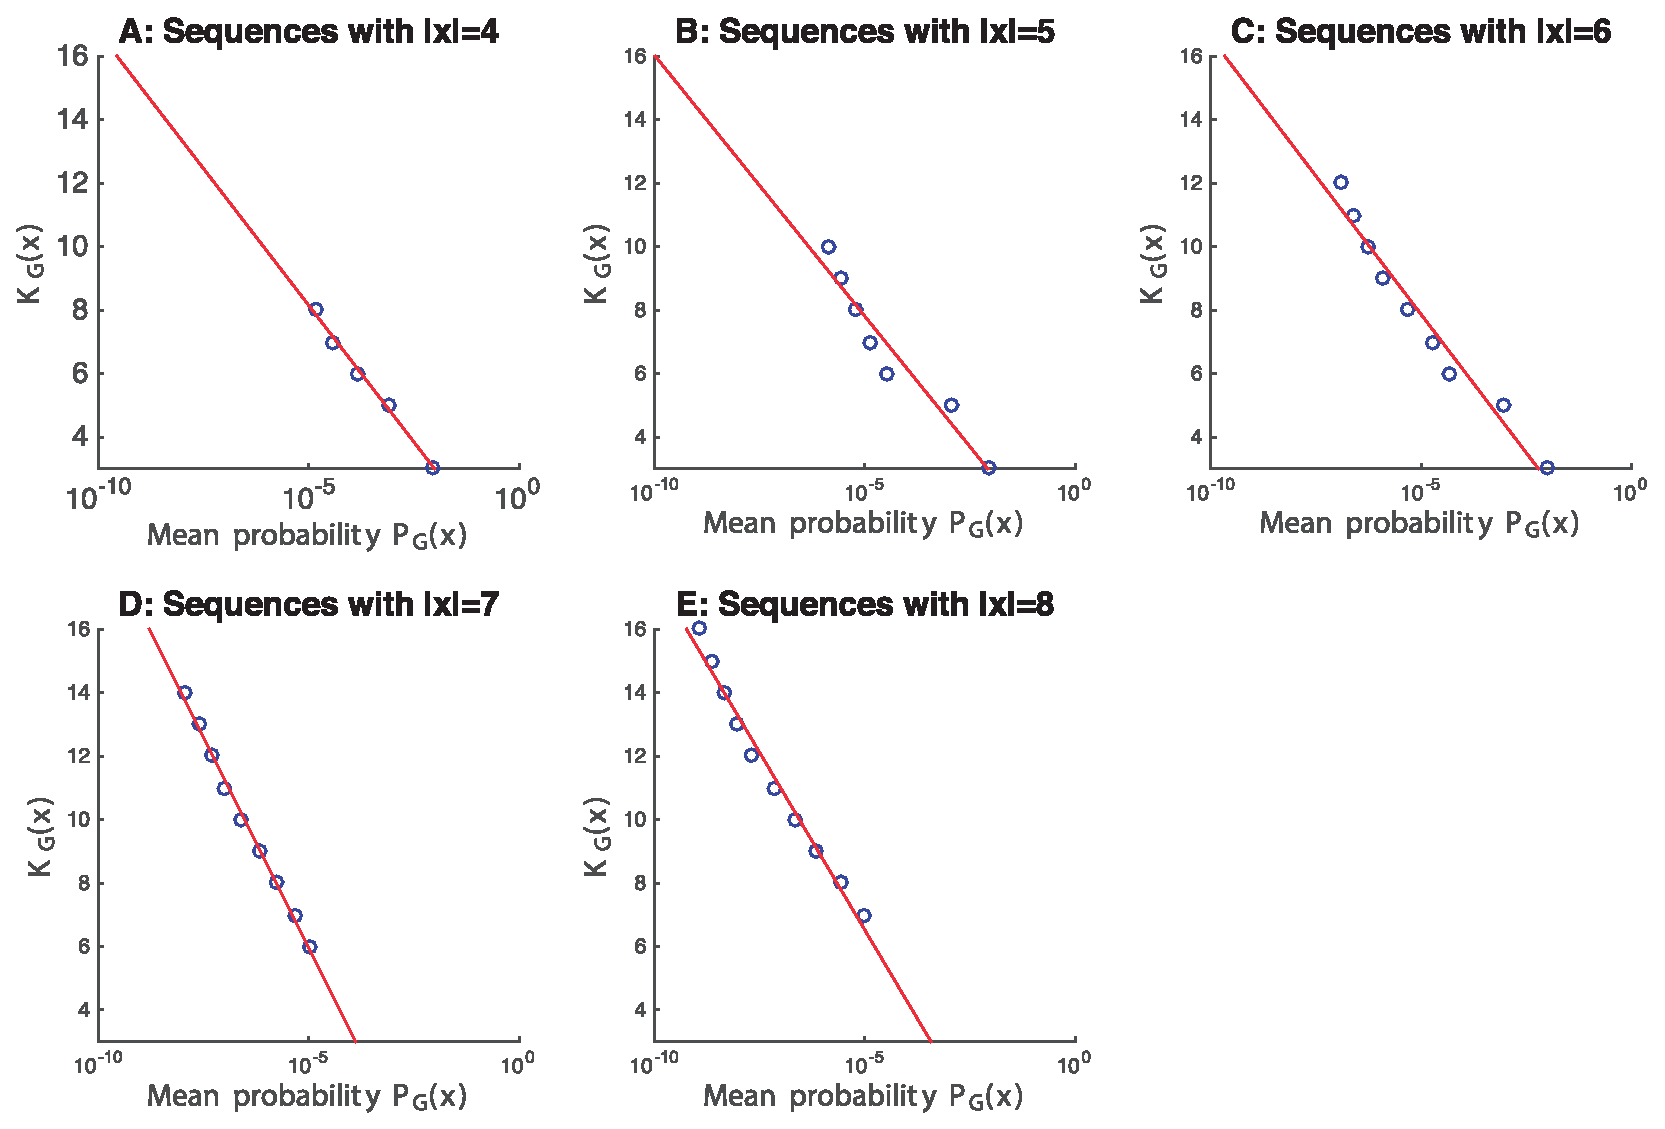
\includegraphics[width=0.4\textwidth]{Fig6}
    \caption{{\bf Probabilidad media $P_{\geom}(x)$.} Probabilidad media $P_{\geom}(x)$ para todas las secuencias $x$ con la misma complejidad.
    Subfigura A: Secuencias con $|x| = 4$.
    Subfigura B: Secuencias con $|x| = 5$.
    Subfigura C: Secuencias con $|x| = 6$.
    Subfigura D: Secuencias con $|x| = 7$.
    Subfigura E: Secuencias con $|x| = 8$.}
    \label{fig:codR}
\end{figure}

%This relationship between the complexity $K_{\geom}$ and the probability $P_{\geom}$ defined for finite sequences in the \textit{language of geometry}, matches the theoretical prediction for infinite sequences in universal languages described in the Coding Theorem. At the same time, it captures the Occam's razor intuition that the simpler sequences one can produce or explain with this language are also the more probable.

Esta relación entre la complejidad $K_{\geom}$ y la probabilidad $P_{\geom}$ definidas para secuencias finitas en el \textit{lenguaje de geometría}, coincide con al predicción teórica para secuencias infinitas en lenguajes universales descrita en el Teorema de Codificación. Al mismo tiempo, captura la intuición de la navaja de Ockham por la cual las secuencias más simples que uno puede producir o explicar en este idioma son también las más probables.

%\figref{fig:codK:8} and \figref{fig:codP:8} show the histogram of $P_{\geom}(x)$ and $K_{\geom}(x)$, respectively, for sequences with length = 8 to get a better insight about both measures. The histogram of the rest of the sequence's lengths are included in \nameref{S2_Fig} and \nameref{S3_Fig} for completeness, and they all show the same behavior.

En \figref{fig:codK:8} y \figref{fig:codP:8} se muestra el histograma de $P_{\geom}(x)$ y $K_{\geom}(x)$, respectivamente, para secuencias de longitud = 8 para obtener una mejor idea de ambas distribuciones. El histograma del resto de las longitudes de la secuencia se incluyen en \nameref{S2_Fig} y \nameref{S3_Fig} por completitud, y todos muestran el mismo comportamiento.

\begin{figure}[!ht]
    \centering
    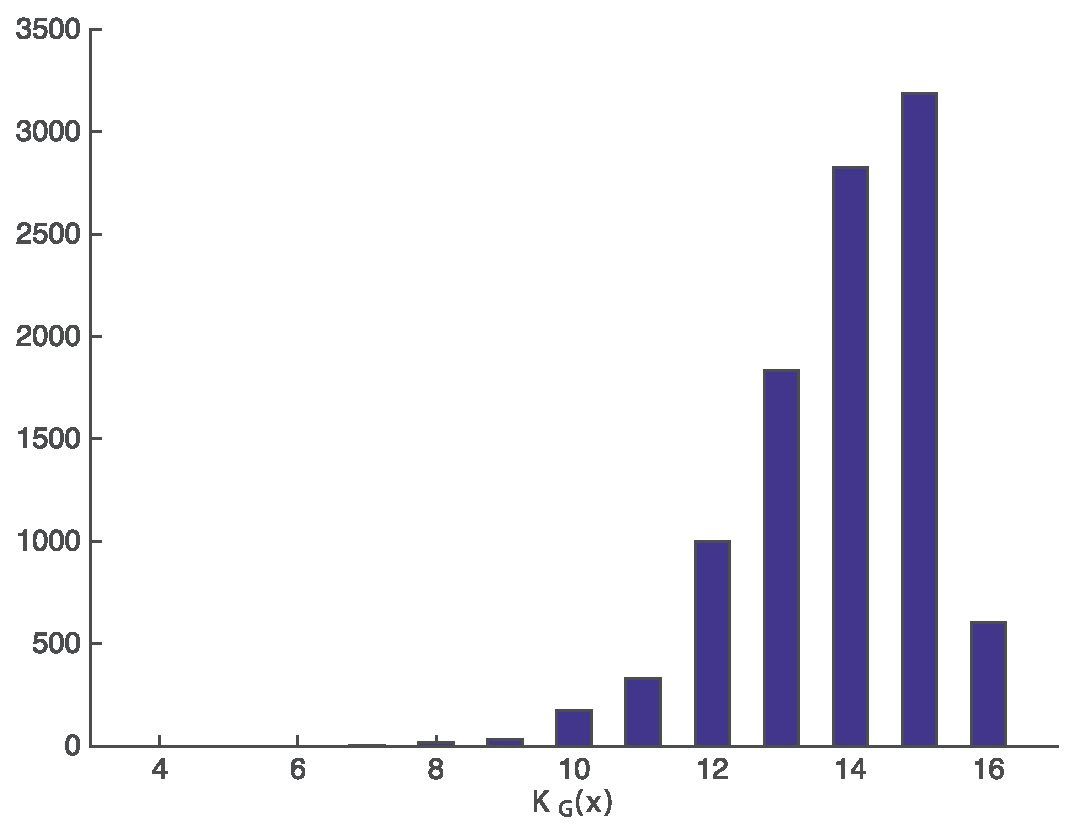
\includegraphics[width=0.4\textwidth]{Fig7}
    %\caption{{\bf Histogram of complexity $K_{\geom}(x)$.} Histogram of complexity for sequences $x$ with $|x| = 8$.}
    \caption{{\bf Histograma de complejidad de $K_{\geom}(x)$.} Histograma de complejidad para secuencias $x$ con $|x| = 8$.}
    \label{fig:codK:8}
\end{figure}


\begin{figure}[!ht]
    \centering
    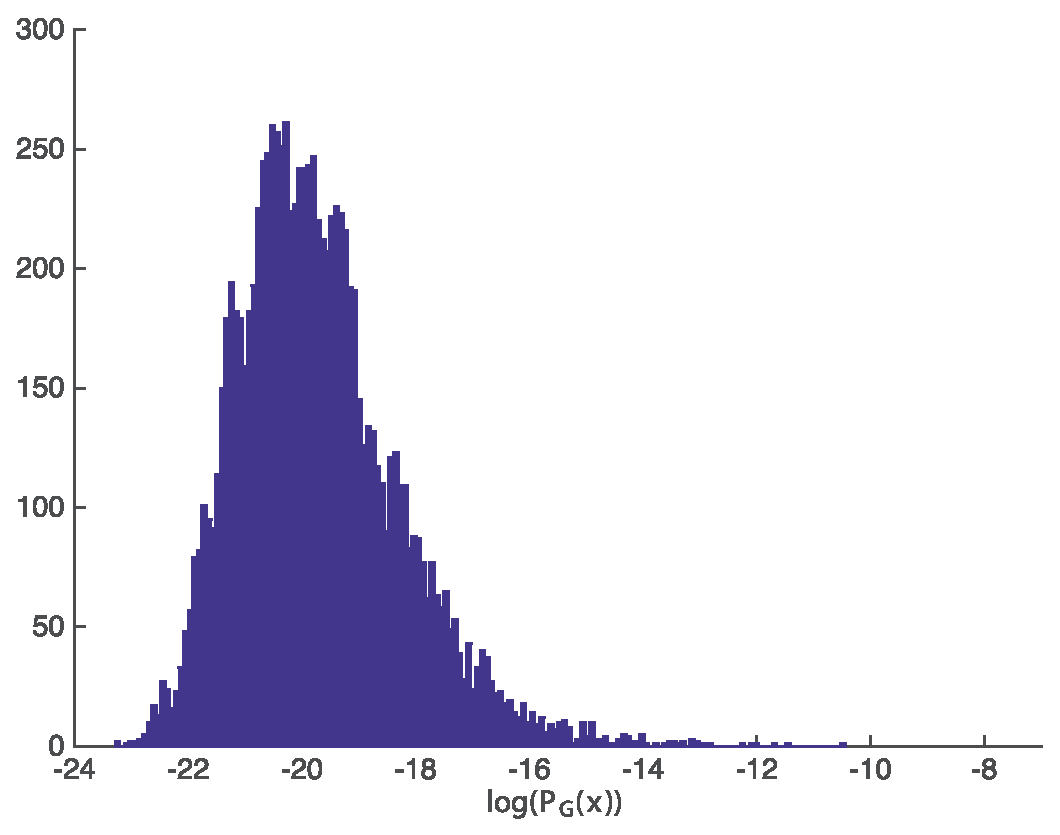
\includegraphics[width=0.4\textwidth]{Fig8}
    %\caption{{\bf Histogram of probability $P_{\geom}(x)$.} Histogram of probability for sequences $x$ with $|x| = 8$.}
    \caption{{\bf Histograma de probabilidad $P_{\geom}(x)$.} Histograma de probabilidad para secuencias $x$ con $|x| = 8$.}
    \label{fig:codP:8}
\end{figure}

%\section{Discussion}
\section{Discusión}

%We have presented a Bayesian inference method to select the set of productions for a LoT and test its effectiveness in the domain of a geometrical cognition task. We have shown that this method is useful to distinguish between arbitrary ad-hoc productions and productions that were intuitively selected to mimic human abilities in such domain.

Hemos presentado un método de inferencia Bayesiano para seleccionar el conjunto de producciones para un LoT y probado su eficacia en el dominio de una tarea de cognición geométrica. Mostramos que este método es útil para distinguir entre producciones ad-hoc arbitrarias y producciones que fueron seleccionadas intuitivamente para imitar las habilidades humanas en ese dominio.

%The proposal to use Bayesian models tied to PCFG grammars in a LoT is not new. However, previous work has not used the inferred probabilities to gain more insight about the grammar definition in order to modify it. Instead, it had usually integrated out the production probabilities to better predict the data, and even found that hierarchical priors for grammar productions show no significant differences in prediction results over uniform priors \cite{piantadosi2012bootstrapping,yildirim2015learning}.

La propuesta de utilizar modelos Bayesianos vinculados a gramáticas PCFG en un LoT no es nueva. Sin embargo, trabajos anteriores no han utilizado las probabilidades inferidas para obtener más información sobre la definición de la gramática y modificarla. En cambio, han integrado usualmente las probabilidades de producción para predecir mejor los datos e incluso se mostró que el uso de distribuciones a priori jerárquicas para las producciones gramaticales no muestran diferencias significativas en los resultados de predicción que al utilizar distribuciones a priori uniformes \cite{piantadosi2012bootstrapping,yildirim2015learning}.

%We believe that inferring production probabilities can help prove the adequacy of the grammar, and can further lead to a formal mechanism for selecting the correct set of productions when it is not clear what a proper set should be. Researchers could use a much broader set of productions than what might seem intuitive or relevant for the domain and let the hierarchical Bayesian inference framework select the best subset.

Creemos que inferir probabilidades de producción puede ayudar a demostrar lo adecuado de una gramática para un dominio, y puede conducir a un mecanismo formal para seleccionar el conjunto correcto de producciones cuando no está claro cuál debería ser el conjunto correcto. Los investigadores podrían utilizar un conjunto de producciones más amplios que aquellas que parezcan intuitivas o relevantes para el dominio y dejar que la inferencia Bayesiana seleccione el mejor subconjunto.

%Selecting a broader set of productions still leaves some arbitrary decisions to be made. However, it can help to build a more robust methodology that --combined with other ideas like testing grammars with different productions for the same task \cite{piantadosi2016logical}-- could provide more evidence of the adequacy of the proposed LoT.

La selección de un conjunto más amplio de producciones todavía deja algunas decisiones arbitrarias por tomar. Sin embargo, puede ayudar a construir una metodología más sólida que --combinada con otras ideas como probar gramáticas con diferentes producciones para la misma tarea \cite{piantadosi2016logical}-- podría proporcionar más evidencia de la idoneidad del LoT propuesto.

%Having a principled method for defining grammars in LoTs is a crucial aspect for their success because slightly different grammars can lead to different results, as has been shown in \cite{piantadosi2016logical}.

Tener un método basado en principios para definir gramáticas en LoTs es un aspecto crucial para su éxito porque gramáticas ligeramente diferentes pueden conducir a resultados muy diversos como se ha demostrado en \cite{piantadosi2016logical}.

%The experimental data used in this work was designed at \cite{marie2016} to understand how humans encode visuo-spatial sequences as structured expressions. As future research, we plan to perform a specific experiment to test these ideas in a broader range of domains. Additionally, data from more domains is needed to demonstrate if this method could also be used to effectively prove whether different people use different LoT productions as outlined in \figref{fig:adultVsChildren}.

Los datos experimentales utilizados en este trabajo fueron diseñados en \cite{marie2016} para comprender cómo los humanos codifican secuencias visuoespaciales como expresiones estructuradas. Como investigaciones futuras, debería realizarse experimentos específicos para probar estas ideas en un rango de dominios más amplios. Además, se necesitan aún más experimentos para probar la efectividad del método para ver si permite individualizar las diferencias de las producciones de los LoTs para distintas poblaciones como se describió en \figref{fig:adultVsChildren}.

%Finally, we showed an empirical equivalence between the complexity of a sequence in a minimal description length (MDL) model and the probability of the same sequence in a Bayesian inference model which is consistent with the theoretical relationship described in the Coding Theorem. This opens an opportunity to bridge the gap between these two approaches that had been described ad complementary by some authors \cite{mackay2003information}.

Finalmente, mostramos una equivalencia empírica entre la complejidad de una secuencia en un modelo de longitud de descripción mínima (MDL) y la probabilidad de la misma secuencia en un modelo de inferencia Bayesiano, lo cual es consistente con la relación teórica descrita en el Teorema de Codificación. Esto abre una oportunidad para cerrar la brecha entre estos dos enfoques que han sido descritos como complementarios por algunos autores \cite{mackay2003information}.


    %%!TEX root = ../main.tex

%\begin{abstract}
%Recent approaches to human concept learning have successfully combined the power of symbolic, infinitely productive rule systems and statistical learning to explain our ability to learn new concepts from  just a few examples. The aim of most of these studies is to reveal the underlying language structuring these representations and providing a general substrate for thought. However, describing a model of thought that is fixed once trained is against the extensive literature that shows how experience shapes concept learning. Here, we ask about the plasticity of these symbolic descriptive languages. We perform a concept learning experiment that demonstrates that humans can change very rapidly the repertoire of symbols they use to identify concepts, by compiling expressions which are frequently used into new symbols of the language. The pattern of concept learning times is accurately described by a Bayesian agent that rationally updates the probability of compiling a new expression according to how useful it has been to compress concepts so far. By portraying the Language of Thought as a flexible system of rules, we also highlight the difficulties to pin it down empirically.
%\end{abstract}

%\chapter{BORRAR: Towards a more flexible Language of Thought: Bayesian grammar updates after each concept exposure}
\chapter{BORRAR: Hacia un lenguaje del pensamiento más flexible: Actualizaciones bayesianas de la gramática tras la exposición a cada concepto}
\chaptermark{Actualizaciones bayesianas tras exposiciones}

\section{Introducción}

%How can children acquire a vast universe of concepts with seemingly very little exposure? One possible solution to this conundrum, known as the Plato Problem~\cite{chomsky1986knowledge,chomsky2006cognitive}, builds on the human capacity to describe concepts --and more generally of all elements of thought-- through the use of a symbolic and combinatorial mental language~\cite{newell1980physical}, referred as {\em language of thought} (LoT)~\cite{fodor1975language}.

¿Cómo pueden los niños adquirir un vasto universo de conceptos con muy poca exposición aparente? Una posible solución a esta pregunta, conocida como el problema de Platón ~\cite{chomsky1986knowledge,chomsky2006cognitive}, se base en la capacidad humana para describir concepto (y en general cualquier elemento del pensamiento) mediante el uso de un lenguaje mental con elementos simbólicos combinatorios~\cite{newell1980physical}, conocido en la literatura como el {\em lenguaje del pensamiento} (LoT, por sus siglas en inglés)~\cite{fodor1975language}.

%Combinatorial languages can describe a vast set of concepts from a small set of primitives. This can be understood in a relatively simple example in the domain of shapes. A combinatorial and symbolic language similar to Logo~\cite{abelson1974logo} can combine operations such as ``move", ``pen up", ``pen down" or ``rotate" to generate an infinite set of expressions (or programs) which, when evaluated, can convey all sort of shapes.

Los lenguajes combinatorios pueden describir un vasto conjunto de conceptos a partir de un pequeño conjunto de primitivas. Podemos entenderlo con un ejemplo relativamente simple en el dominio de las formas. Un lenguaje combinatorio similar a Logo ~\cite{abelson1974logo} puede combinar símbolos de operaciones como ``mover", ``lápiz arriba", ``lápiz abajo" o ``rotar" para generar un conjunto infinito de expresiones (o programas) que, cuando se evalúan, pueden trasmitir todo tipo de formas.

%A language describing concepts (like shapes) also provides a natural notion of their complexity \cite{kolmogorov1968three}. A concept is simple, relative to that language, when it can be described by a short program. On the contrary, it is complex when all its descriptions require a long sequence of instructions. For example, in the case of the Logo language, a square can simply be instructed as a loop of four displacements followed by rotations of 90 degrees. In this language, the icon of a face will be implemented by a significant lengthier program and hence will be more complex.  However, this concept would be simpler when described in a language in which the icon of a face (or the symbols for nose, mouth, etc.) are available as primitives in the language.

Un lenguaje que describe conceptos (como las formas) también proporciona una noción natural de su complejidad \cite{kolmogorov1968three}. Un concepto es simple, relativo a ese lenguaje, cuando puede ser descrito por un programa corto. Por el contrario, es complejo cuando todas sus descripciones requieren una larga secuencia de instrucciones. Por ejemplo, en el caso de Logo, un cuadrado se puede instrumentar simplemente como un bucle de cuatro desplazamientos seguidos de rotaciones de 90 grados. En cambio, describir una cara requerirá de un programa más largo y, por lo tanto, será un concepto más complejo de describir. Sin embargo, este concepto se podría describir de manera más simple en un lenguaje en el que el icono de una cara (o de una nariz, boca, etc.) estuvieran disponibles como primitivas de ese lenguaje. 

%In the domain of Boolean concepts, a wide range of logical varieties of concepts was studied in~\cite{feldman2003simplicity}, revealing a surprisingly simple `law': the subjective difficulty of a Boolean concept for a human learner is directly proportional to the length of the shortest compatible program in the language of propositional logic (i.e.\ Boolean variables combined with the operators \textit{and}, \textit{or} and \textit{not}). This result may suggest that human LoT is equipped with rules and symbols similar to those found in propositional logic. Indeed, the correlation between the subjective difficulty of concepts and their complexity has been used as a general vehicle to study human LoT in various domains ~\cite{piantadosi2016logical,leeuwenberg1971perceptual,amalric2017language,romano2018,lupyan2007language}. Although often implicit, the general strategy is to (\textit{1)} assume a language; (\textit{2)} find the shortest compatible program for some concepts in that language; (\textit{3)} compare the length of these programs with the subjective difficulty of the concepts; and finally (\textit{4)} repeat this process for various languages within a universe of possible candidates and choose the language that gives the best match in \textit{(3)}. As mentioned before, the length of the program depends on the primitives of the language in which this program is written, so different languages make different predictions.

En el dominio de los conceptos Booleanos, se ha estudiado una amplia variedad de conceptos lógicos~\cite{feldman2003simplicity}, revelando una `ley' sorprendentemente simple: la dificultad subjetiva de aprender un concepto Booleano para un humano es directamente proporcional a la longitud del programa compatible más corto en el lenguaje de la lógica proposicional (es decir, a un lenguaje con símbolos para variables Booleanas que pueden combinarse con los operadores \textit{y}, \textit{o} y \textit{no}). Este resultado puede sugerir que el LoT está equipado con reglas y símbolos similares a los que se encuentran en la lógica proposicional. En general, la correlación entre la dificultad subjetiva de los conceptos y su complejidad se ha utilizado como un mecanismo general para estudiar el LoT en varios dominios ~\cite{piantadosi2016logical,leeuwenberg1971perceptual,amalric2017language,romano2018,lupyan2007language}. Aunque a menudo sea de forma implícita, la estrategia general en estos trabajos es: (\textit{1)} asumir un lenguaje; (\textit{2)} encontrar el programa compatible más corto para algunos conceptos en ese lenguaje; (\textit{3)} comparar la longitud de estos programas con la dificultad subjetiva de los conceptos; y finalmente, (\textit{4)} repetir ese proceso para varios lenguajes dentro de un universo de posibles candidatos y elegir el lenguaje que ofrezca la mejor coincide en \textit{(3)}. Como se mencionó anteriormente, la duración del programa depende de las primitivas del lenguaje en el que está escrito ese programa, por lo tanto, diferentes idiomas implican diferentes predicciones.

%A natural question, however, is whether the primitives of a LoT are universal --both across different individuals and also throughout development-- or if instead the semantic repertoire of a language is dynamic and shaped by experience. Indeed, it is likely that our ability to automatically represent Boolean concepts in a succinct manner is not due to an innate efficient propositional language in our mind. Instead, we propose that this ability arises as a byproduct of our brain rapidly learning efficient representations for the concepts we usually  encounter in everyday life. Our research question is: how rapidly can we adapt our learning mechanisms when we encounter a new domain in which our a priori representations are no longer efficient? We examine the hypothesis that humans have the ability to rapidly recombine propositions in their LoT, adding new primitives to their language. In other words, that learning leads to a process of compiling routines into functions within the LoT.

Sin embargo, una pregunta natural es si las primitivas de un LoT son universales, tanto a través de diferentes individuos como también a lo largo del desarrollo. O si en cambio, el repertorio de símbolos de un lenguaje es dinámico y está moldeado por la experiencia. De hecho, es probable que nuestra capacidad para representar automáticamente conceptos Booleanos de una manera sucinta no se deba a a un lenguaje proposicional eficiente innato en nuestra mente. En cambio, es probable que esta habilidad surja como un subproducto de que nuestro cerebro aprende rápidamente representaciones eficientes para los conceptos que solemos encontrar en la vida cotidiana. La pregunta que guía este capítulo es: ¿Qué tan rápido podemos adaptar nuestros mecanismos de aprendizaje cuando nos encontramos con un nuevo dominio en el que nuestras representaciones a priori ya no son eficientes? Examinamos la hipótesis de que los humanos tienen la capacidad de recombinar rápidamente proposiciones en su LoT, agregando nuevas primitivas al lenguaje. En otras palabras, ese aprendizaje conduce a un proceso de compilación de rutinas en nuevos símbolos de funciones dentro del LoT.

%In the example of the Logo language one can imagine that if productions which draw squares are very frequent, it would be efficient to devote a new symbol to this production. The new symbol `square' is a hierarchical `second order' construction of the `first order' primitives of the language. It has a cost (of increasing the lexicon of the language) but in the new language, drawing a square can be instantiated with a very short program (namely, `square') and hence uses less memory. Indeed, a higher level language allows us to reach a higher level of abstraction by freeing memory and processing power, thus making more complex thoughts thinkable~\cite{minsky1967computation,murphy1988comprehending}.

En el ejemplo del lenguaje Logo, uno puede imaginar que si las producciones que dibujan los cuadrados son muy frecuentes, entonces ería conveniente dedicar un nuevo símbolo a esta producción. El nuevo símbolo `cuadrado' es una construcción jerárquica de `segundo orden' construido a partir de las primitivas de `primer orden' del lenguaje. Incrementar los símbolos del lenguaje tiene un costo, pero en el nuevo lenguaje, dibujar un cuadrado puede ser instrumentado con un programa muy corto (simplemente, `cuadrado') y, por tanto, utilizando menos memoria. De esta manera, un lenguaje de nivel superior nos permite alcanzar un mayor nivel de abstracción al liberar memoria y potencia de procesamiento, haciendo así que pensamientos más complejos puedan pensarse~\cite{minsky1967computation,murphy1988comprehending}.

%Most work in the LoT literature, while naturally including a learning mechanism, tends to approach the LoT as a stable system to be unearthed by experimenters, who try different candidate templates and select the one which best fits the data after training ~\cite{goodman2008rational,kemp2012exploring,piantadosi2016logical}. Still, how different tracks of experience can shape acquisition differently and can constantly change the repertoire of a LoT after each exposure remains to be discovered.

La mayoría del trabajo en la literatura sobre LoT, aunque naturalmente incluye un mecanismo de aprendizaje, tiende a abordar al LoT como un sistema estable para ser descubierto por los experimentadores, que prueban diferentes plantillas de posibles candidatos y seleccionan aquel que mejor se ajuste a los datos de entrenamiento ~\cite{goodman2008rational,kemp2012exploring,piantadosi2016logical}. Sin embargo, cómo diferentes trayectorias de experiencia pueden moldear distintos lenguajes y cómo pueden cambiar de manera continua el repertorio de símbolos de un LoT después de cada exposición queda todavía por descubrirse.

%Here, we perform a Boolean concept learning experiment to show that humans can change very rapidly --in the course of an experiment-- the repertoire of symbols they use to identify concepts. We also provide a dynamic model that is flexible enough to update its underlying language after each concept exposure. 

En este capítulo realizamos un experimento de aprendizaje de conceptos Booleanos para demostrar que los humanos pueden cambiar muy rápidamente, en el curso de un mismo experimento, el repertorio de símbolos que utilizan para identificar conceptos. También proporcionamos un modelo dinámico que es lo suficientemente flexible para actualizar su lenguaje subyacente después de cada exposición a un concepto.

%In our experiment, participants are divided in two groups, in such a way that each group is presented with a different sequence of concepts. One of the two groups is presented with concepts that are succinctly described only if the logical operator `exclusive or' (xor, notated~$\oxor$) is used, which we presume does not form part of the natural repertoire of LoT in this specific domain~\cite{piantadosi2016logical}. However, these concepts can also be described with a sensibly lengthy combination of primitives excluding $\oxor$. We show how the exposure to this set of concepts `compiles' the $\oxor$ operator in a way that, after exposure, subjective difficulty is described by an extended language in which $\oxor$ has been incorporated to the set of primitives. Furthermore, we show that the subjective difficulty of concepts throughout the task is consistent with that of a Bayesian agent that rationally updates the probability of compiling $\oxor$ according to how useful it has been to compress concepts so far.

En nuestro experimento, los participantes se dividen en dos grupos de tal manera que a cada grupo se le presenta una secuencia diferente de conceptos. Uno de los dos grupos observa conceptos que pueden describirse de manera sucinta sólo si se utiliza el operador lógico `o exclusivo' (xor, anotado ~$\oxor$), el cual asumimos no forma parte del repertorio natural del LoT en este dominio específico~\cite{piantadosi2016logical}. Sin embargo, estos conceptos también se pueden describir con una combinación sensiblemente más larga de primitivas que excluyen al $\oxor$. Mostramos como la exposición a este conjunto de conceptos para el grupo `compila' el operador $\oxor$ de tal manera que ---después de la exposición--- la dificultad subjetiva es descripta de mejor manera por una versión extendida del lenguaje en el cual $\oxor$ ha sido incorporado al conjunto de primitivas. Además, mostramos que la dificultad subjetiva de los conceptos a lo largo del experimento es consistente con la de un agente Bayesiano que actualiza racionalmente la probabilidad de compilar $\oxor$ de acuerdo a qué tan útil ha sido para comprimir los conceptos vistos hasta ese momento.

%\section{The logical setting}
\section{La configuración Booleana}

%We consider two propositional logics, both containing only four  propositional variables $\vars=\{x_1, x_2, x_3, x_4\}$. \grambool is defined over the signature $\oand$, $\oor$ and $\lnot$, and \gramboolxor is defined over the signature $\oand$, $\oor$, $\lnot$ and $\oxor$. As one can see from the grammars defined in Fig.~\ref{PCFG}, the only difference between \grambool and \gramboolxor is that the latter has an additional operator $\oxor$.  

Consideramos dos lógicas proposicionales, ambas contienen sólo cuatro variables proposicionales  $\vars=\{x_1, x_2, x_3, x_4\}$. \grambool se define con los operadores $\oand$, $\oor$ y $\lnot$, y \gramboolxor se define con los operadores $\oand$, $\oor$, $\lnot$ y $\oxor$. Como se puede ver en las gramáticas definidas en la Figura~\ref{PCFG}, la única diferencia entre \grambool y \gramboolxor es que la última tiene un operador adicional: $\oxor$.  
 \begin{figure}[h!]
\centering
\small\vspace{-.3cm}
\begin{tabular}{ccc}
\begin{minipage}[h]{0,2\textwidth}
\begin{eqnarray*}
\start &\to&\bool\\
\bool &\to&(\bool \oand \bool) \\
\bool &\to&(\bool \oor \bool) \\
\bool &\to&\atom
\end{eqnarray*}
\end{minipage}
&
\ \quad
&
\begin{minipage}[h]{0,2\textwidth}
\ \quad Para $i=1,2,3,4$
\begin{eqnarray*}
\atom &\to& x_i \\
\atom &\to&\lnot x_i 
\end{eqnarray*}
\end{minipage}
\end{tabular}
      %\caption{The context free grammar for language \grambool.  Language \gramboolxor has an extra rule: $\bool\  \to\ (\bool \oxor \bool)$}
      \caption{La gramática libre de contexto para el lenguaje \grambool.  El lenguaje \gramboolxor tiene una producción extra: $\bool\  \to\ (\bool \oxor \bool)$}
      \label{PCFG}
   \end{figure}

\santi{toda esta parte de semantica y MDL puede ir en intro. Es comun con el trabajo de BRM. Acá está con más detalle que en BRM}

%The semantics of $\oand$, $\oor$ and $\lnot$ are standard: conjunction, disjunction and negation, respectively. We let $\oxor$ denote the exclusive disjunction. As usual, $v\models \varphi$, represents that the formula $\varphi$ is true for the valuation $v:\vars\to\{0,1\}$ and we denote the {\em semantics} of $\varphi$ by $\sem{\varphi}=\{v\colon v\models\varphi\}$. A {\em concept} $\con$ is a set of valuations $\vars\to\{0,1\}$. The complement of $\con$ is denoted $\overline \con$ and is defined as $\overline \con=\{0,1\}^\vars\setminus \con$. Observe that $\#\con+\#\overline \con=16$. We say that a formula $\varphi$ is {\em compatible} with concept $\con$ if $\sem{\varphi}=\con$. We regard logics as languages for describing concepts. Any concept $\con$ has infinitely many descriptions, namely, all formulas $\varphi$ such that $\sem{\varphi}=\con$. 

La semántica de $\oand$, $\oor$ y $\lnot$ son estándar: conjunción, disyunción y negación, respectivamente. Mientras que $\oxor$ denota la disyunción exclusiva. Como de costumbre, $v\models \varphi$, representa que la formula $\varphi$ es verdadera para la valuación $v:\vars\to\{0,1\}$ y denotamos la {\em semántica} de $\varphi$ con $\sem{\varphi}=\{v\colon v\models\varphi\}$. Un {\em concepto} $\con$ es un conjunto de valuaciones $\vars\to\{0,1\}$. El complemento de $\con$ se denota $\overline \con$ y se define como $\overline \con=\{0,1\}^\vars\setminus \con$. Observar que $\#\con+\#\overline \con=16$. Decimos que una fórmula $\varphi$ es {\em compatible} con el concepto $\con$ si $\sem{\varphi}=\con$. De esta manera, consideramos la lógica proposicional como un lenguaje para describir conceptos. Cualquier concepto $\con$ tiene entonces infinitas descripciones: todas las fórmulas $\varphi$ tal que $\sem{\varphi}=\con$. 

\paragraph*{Ejemplo.}
%In Fig.~\ref{semaforos} we depict a concept $\con$ (variables are represented by colors) such that $\#\con=4$. One can see that the formula $x_3$ is not compatible with $\con$ but $x_1 \oand x_2$, or $x_1 \oand x_2 \oand (x_3 \oor \lnot x_3)$, are compatible with $\con$. $\overline \con$ may be described by $\lnot x_1\oor \lnot x_2$.
En la Figura~\ref{semaforos} representamos un concepto $\con$ (las variables están representadas por colores) tal que $\#\con=4$. Se puede ver que la fórmula $x_3$ no es compatible con $\con$ pero $x_1 \oand x_2$, o $x_1 \oand x_2 \oand (x_3 \oor \lnot x_3)$, sí son compatibles con $\con$. $\overline \con$ puede describirse mediante $\lnot x_1\oor \lnot x_2$.

%We will often identify concepts with any formula compatible with it, so we will talk of ``concept $\varphi$'' to refer to ``concept $\sem{\varphi}$''. However, it should be noted that a concept is a semantic object that has many descriptions in the logical language.

A menudo identificaremos conceptos con cualquier fórmula compatible con ella, por lo que hablaremos de ``concepto $\varphi$'' para referirnos a ``concepto $\sem{\varphi}$''. Sin embargo, cabe señalar que un concepto es un objeto semántico que tiene muchas descripciones en el lenguaje.

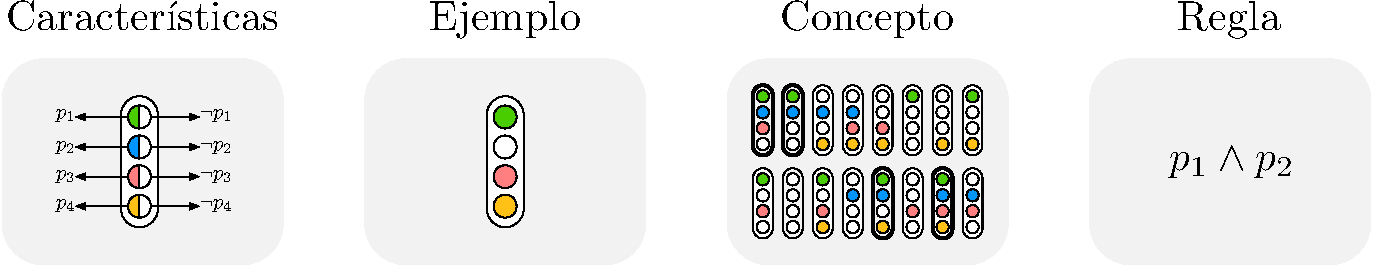
\includegraphics[scale=.6]{../figuras/pre/notacion.pdf}
\widesanti{Sergio, esta imagen es nueva. Pienso que puede dar coherencia con BRM. Puede remplazar a la figura anterior. Hay que actualizar notación en el texto y cambiar $x_i$ por $p_i$, etc. Cuando se presente la figura análoga en BRM, podes mandar un cf. a esta}

%A lower bound for the complexity of a concept in a given logic corresponds to the shortest description of that concept, that is, its minimum description length (MDL).
Un límite inferior para la complejidad de un concepto en una lógica dada corresponde a la descripción más corta de ese concepto, es decur, su longtud mínima de descripción (MDL).

 \begin{figure}[t!]
 \vspace{-0.5cm}
  \centering
  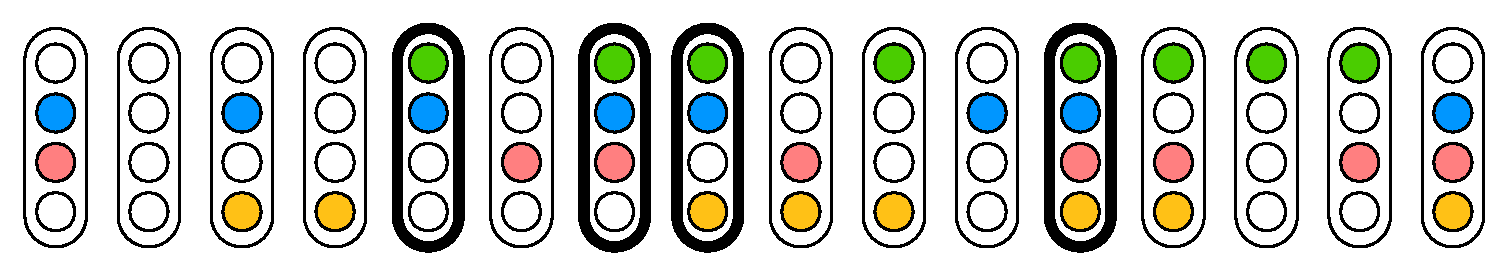
\includegraphics[scale=.335]{semaforos2.pdf}
  %\caption{Example of a concept $\con$, as shown in the experiment. Variables in $\vars=\{x_1,x_2,x_3,x_4\}$ correspond to the presence of a  color light in the object ($x_{1}=$ green, $x_2=$ blue, $x_3=$ red, $x_4=$ orange). Items (valuations) belonging to $\con$ are highlighted with bold border. $\con$ may be described by $x_1\oand x_2$. As in a traffic light, each color is fixed to each position.}
  \caption{Ejemplo de un concepto $\con$, como se muestra en el experimento. Variables en $\vars=\{x_1,x_2,x_3,x_4\}$ corresponden a la presencia de una luz de color en el objeto ($x_{1}=$ verde, $x_2=$ azul, $x_3=$ rojo, $x_4=$ naranja). Los objetos (valuaciones) que pertenecen a $\con$ se resaltan con un bordo en negrita. $\con$ puede describirse mediante $x_1\oand x_2$. Como en un semáforo, cada color está fijado siempre en la misma posición.}
  \label{semaforos}
\end{figure}
   
%The {\em size} of a formula $\varphi$ is denoted $|\varphi|$ and it is defined as the number of operators plus the number of atoms (i.e.\ possibly negated propositional symbols), that is: $|x_i|=|\lnot x_i|=1$ for $i=1\dots 4$ and $|\varphi_1*\varphi_2|=|\varphi_1|+|\varphi_2|+1$ for $*\in\{\oand,\oor,\oxor\}$. For ${\sf L} \in\{\grambool,\gramboolxor\}$ and a concept $\con$ we define the {\em minimum description length of $\con$ with respect to $\mathcal {\sf L}$} as
El {\em tamaño} de una fórmula $\varphi$ se denota como $|\varphi|$ y se define como el número de operadores más el número de átomos (símbolos proposicionales posiblemente negados), es decir: $|x_i|=|\lnot x_i|=1$ para $i=1\dots 4$ y $|\varphi_1*\varphi_2|=|\varphi_1|+|\varphi_2|+1$ para $*\in\{\oand,\oor,\oxor\}$. Para ${\sf L} \in\{\grambool,\gramboolxor\}$ y un concepto $\con$ definimos la {\em la longitud mínima de descripción de $\con$ con respecto a $\mathcal {\sf L}$} como:
$$
\mdl{\sf L}(\con)=\min\{|\varphi|\colon \varphi\in\mathcal L, \sem{\varphi}=\con\}.
$$
Como $\grambool$ es un sublenguaje de $\gramboolxor$, tenemos que $\mdl{\gramboolxor}(\con)\leq\mdl{\grambool}(\con)$ para cualquier concepto $\con$.
   
\paragraph*{Ejemplo.}El concepto $
\con=\{v\colon v(x_1)+v(x_2)=1\},
$
%which expresses that $x_1$ is true or $x_2$ is true but not both can be described in \gramboolxor as $\varphi=x_{1} \oxor x_{2}$, of length 3. In fact, one can check that this is the shortest formula compatible with $\con$, and so $\mdl{\gramboolxor}(\con)=3$. If we now switch to \grambool, we can no longer describe $\con$ as $x_{1} \oxor x_{2}$, since $\oxor$ is not part of its signature. However, in \grambool, the concept $\con$ may be described by  formula $\psi=(x_{1} \oand \neg x_{2}) \oor (x_{2} \oand \neg x_{1})$, of size 7. Since this formula has minimal size, we have that $\mdl{\grambool}(\con)=7$.
que expresa que $x_1$ es verdadero o $x_2$ es verdadero, pero no ambas puede describirse en \gramboolxor como $\varphi=x_{1} \oxor x_{2}$, de tamaño 3. De hecho, se puede comprobar que esta es la fórmula más corta compatible con $\con$, por lo que $\mdl{\gramboolxor}(\con)=3$. Si ahora cambiamos a \grambool, ya no podemos describir a $\con$ como $x_{1} \oxor x_{2}$, dado que $\oxor$ no es parte del lenguaje. Sin embargo, en \grambool, el concepto $\con$ puede describirse mediante la fórmula $\psi=(x_{1} \oand \neg x_{2}) \oor (x_{2} \oand \neg x_{1})$, de tamaño 7. Dado que esta fórmula tiene tamaño mínimo para ese concepto en \grambool, tenemos que $\mdl{\grambool}(\con)=7$.

\section{Experimento}


\renewcommand*{\arraystretch}{1.2}
   
\begin{table*}[!ht]
\vspace{-0.5cm}
\centering

\begin{tabular}{|c|l l | c | c |l l | c | c|}
\hline
                                   &
\multicolumn{2}{c|}{\textbf{Grupo objetivo}}       &
\textbf{$\mdl{\gramboolxor}(\con)$} &
\textbf{$\mdl{\grambool}(\con)$} &
\multicolumn{2}{c|}{\textbf{Grupo control}}  &
\textbf{$\mdl{\gramboolxor}(\con)$} &
\textbf{$\mdl{\grambool}(\con)$} 
 \\ \hline
\multirow{4}{*}{\parbox[t]{2mm}{\rotatebox[origin=c]{90}{\bf Entrenamiento}}} & \targeta & $x_{i}$             & 1 & 1                                                                  & \multicolumn{4}{c|}{$\longleftarrow$Ídem}                                                            \\ \cline{2-9}
                                   &\targetb& $x_{i} \oxor x_{j}$       & 3 & 7 &\controlb& $x_{i} \oor x_{j}$  & 3 & 3                                                                  \\ \cline{2-9}
                                  &\targetc & $x_{i} \oxor x_{j} \oxor x_{k}$ & 5 & 19 &\controlc& $x_{i} \oor (x_{j} \oand x_{k})$  & 5 & 5 \\ \cline{2-9}
                                  &\targetd& $x_{k} \oxor x_{l}$       & 3 & 7&\controld&$x_{k} \oor x_{l}$  & 3 & 3                                                                  \\ \hline
\multirow{2}{*}{\parbox[t]{2mm}{\rotatebox[origin=c]{90}{\bf Evaluación}}}  &\testa& $x_{i} \oand (x_{j} \oxor x_{k})$ & 5 & 9                 & \multicolumn{4}{c|}{$\longleftarrow$Ídem}                                                                                    \\ \cline{2-9}
                               &\testb& $x_{i} \oand (x_{j} \oor x_{k})$  & 5 & 5         & \multicolumn{4}{c|}{$\longleftarrow$Ídem}                                                                                            \\ \hline
\end{tabular}

\caption{Secuencia de conceptos presentados en el experimento: \targeta, \targetb, \targetc, \targetd, \testa, \testb para el grupo objetivo y  \controla, \controlb, \controlc, \controld, \testa, \testb para el grupo control. Cada concepto $\con$ está representado por una fórmula mínima $\varphi$ tal que $\sem{\varphi}=\con$. %Numbers $n/m$ on the right indicate $n=\mdl{\gramboolxor}(\con)$ and $m=\mdl{\grambool}(\con)$.
%MDL is measured as the number of operators and variables (excluding the \textit{not} operator) of the minimal formula with respect to the specified CFG.
}
\label{conceptos}
\vspace{-0.4cm}
\end{table*}



\begin{table}[]\small
\begin{tabular}{|c|c||c|c|c||c|c|c|}
\hline
\textbf{}                 & \textbf{Prueba} & \textbf{\begin{tabular}[c]{@{}c@{}}Grupo\\ Objetivo\end{tabular}} & \textbf{$\mdl{\gramboolxor}$} & \textbf{$\mdl{\grambool}$} & \textbf{\begin{tabular}[c]{@{}c@{}}Grupo\\ Control\end{tabular}} & \textbf{$\mdl{\gramboolxor}$} & \textbf{$\mdl{\grambool}$} \\ \hline
\multirow{4}{*}{\parbox[t]{2mm}{\rotatebox[origin=c]{90}{\bf Entrenamiento\ \ \ \ \ \\ \ \  }}} & 1               & \begin{tabular}[c]{@{}c@{}}\targeta \\ $x_{i}$\end{tabular}                     & 1              & 1               & \multicolumn{3}{c|}{$\longleftarrow$ ídem}                                                                           \\ \cline{2-8} 
                          & 2               & \begin{tabular}[c]{@{}c@{}}\targetb\\ $x_{i} \oxor x_{j}$\end{tabular}                     & 3              & 7               & \begin{tabular}[c]{@{}c@{}}\controlb\\ $x_{i} \oor x_{j}$\end{tabular}                    & 3              & 3               \\ \cline{2-8} 
                          & 3               & \begin{tabular}[c]{@{}c@{}}\targetc \\ $x_{i} \oxor x_{j} \oxor x_{k}$\end{tabular}                     & 5              & 19              & \begin{tabular}[c]{@{}c@{}}\controlc\\ $x_{i} \oor (x_{j} \oand x_{k})$\end{tabular}                    & 5              & 5               \\ \cline{2-8} 
                          & 4               & \begin{tabular}[c]{@{}c@{}}\targetd\\ $x_{k} \oxor x_{l}$\end{tabular}                     & 3              & 7               & \begin{tabular}[c]{@{}c@{}}\controld\\$x_{k} \oor x_{l}$\end{tabular}                    & 3              & 3               \\ \hline
\multirow{2}{*}{\parbox[t]{2mm}{\rotatebox[origin=c]{90}{\bf Evaluación}}}     & 5               & \begin{tabular}[c]{@{}c@{}}\testa\\ $x_{i} \oand (x_{j} \oxor x_{k})$\end{tabular}                     & 5              & 9               & \multicolumn{3}{c|}{$\longleftarrow$ ídem}                                                                           \\ \cline{2-8} 
                          & 6               & \begin{tabular}[c]{@{}c@{}}\testb\\ $x_{i} \oand (x_{j} \oor x_{k})$\end{tabular}                     & 5              & 5               & \multicolumn{3}{c|}{$\longleftarrow$ ídem}                                                                           \\ \hline
\end{tabular}
\end{table}
\widesanti{hice esta tabla como la anterior pero con diseño para que entre. Si te gusta y la querés cambiar, adelante. Solo que antes hay que revisar que tenga los mismos datos!}


\widesanti{habría que unificar con BRM las x con las p}

55 participants participated in the experiment over the world wide web using the Amazon Mechanical Turk crowd sourcing platform. All were US residents over the age of 18 and had more than 95\% of past tasks successfully approved by other requesters. 44 participants completed the experiment through all the stages and declared not cheating (using pen, screenshots or a similar method to copy the answers) at the end of the experiment. Only data from these participants were used in the analyses reported below.\footnote{The learning times of all participants can be found in https://figshare.com/s/04d338adbbc4b1e83bf0.}

Participants were divided randomly into a control group ($N=21$) and a target group ($N=23$). Both groups were presented with different sequences of six concepts. For each concept, there was a learning phase, a testing phase and a feedback phase. The average time spent in each concept was 167$\pm$20 s.e.m.\ seconds, and the average duration of the task was 21$\pm$4 s.e.m.\ minutes. After moving through the learning, testing and feedback phase of each of the six concepts, participants were asked if they used a pen or recorded the screen information in any way. They were also told that the answer to this question will not affect their payment, but that it was crucial for the experimenters to know.


During the learning phase, all 16 items were presented in the screen (in random order), and items belonging to the concept were identified with bold boundaries, as shown in  Fig.~\ref{semaforos}.
Participants were told that only the items with bold boundaries were `blickets' (or `tufas', etc.: we used different words for each concept in the sequence), and asked them to try to identify what a blicket was. During the testing phase, the 16 items were shuffled in the screen, and participants were asked to click on items that were blickets. If they made mistakes after submitting their answer, they were directed to the feedback phase, in which items that were incorrectly classified were indicated with a red cross. After having studied the feedback, participants were redirected to the testing screen, where items were reshuffled. When every item was correctly classified, participants were asked to give a verbal description of the concept and then continued on to the following concept after a resting period. We characterize the subjective difficulty of each concept as the time the participant spent in learning, testing and feedback phases for that concept (excluding the time spent in the verbal description).


\begin{figure}
\begin{center}
  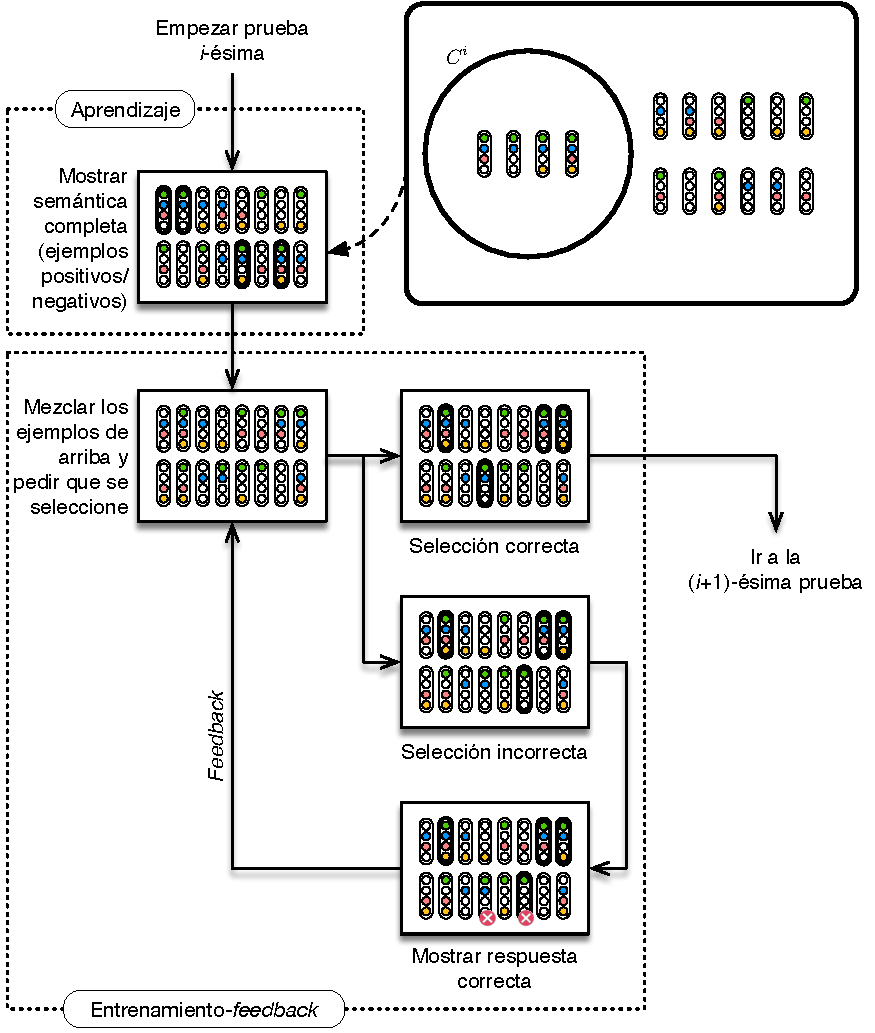
\includegraphics[scale=1]{../figuras/pre/experimento_PRE.pdf}
\end{center}\caption{}
\end{figure}
\widesanti{Sergio, esta figura es nueva. Es una adaptación de la de BRM, más simple y con los ejemplos de semáforos. Pienso que puede dar más coherencia a la tesis. Podés confrontarla desde el capítulo de BRM y decir que en BRM es más complejo: (a) mostramos semantica INCOMPLETA (b) hay 2 conceptos en vez de 1 y (c) hay una etapa de GENERALIZACION}

Both groups (target and control), were exposed to 6 concepts. The second, third and fourth concepts are {\em training} concepts, and were different between both groups. The last two concepts are the {\em test} concepts, and were the same for both groups. The first concept was the trivial concept $x_i$ for both groups, which was aimed to get participants started in the task. Importantly, variables (i.e. color lights inside objects in Fig.~\ref{semaforos}) were randomized for every concept, so paying selective attention to a specific variable across subsequent concepts was not beneficial for learning the concept sequence.


As shown in Table~\ref{conceptos}, we presented the target group with training concepts which are succinctly described when $\oxor$ is part of the language, but necessarily described with lengthier formulas if $\oxor$ is absent; more technically, concepts for which $\mdl{\gramboolxor}$ is much smaller than $\mdl{\grambool}$. We also corroborated that for \targetb, \targetc, \targetd and \testa the number of formulas in $\gramboolxor$ with length strictly smaller than $\mdl{\grambool}$ was at least 10 times greater than the number of formulas in $\grambool$ with length equal to $\mdl{\grambool}$.

Participants in the control group, on the other hand, experienced a sequence of concepts that could be easily described using the language given by \grambool. After these training concepts, both groups were presented with the same pair of test concepts: one which could be only succinctly described in \gramboolxor, and one for which the MDL did not depend on the underlying language \gramboolxor or \grambool. We compared learning times between the two groups for these last two concepts.


As shown in Table~\ref{conceptos}, training concepts for the target (xor) group were: $x_{i}$, $x_{i} \oxor x_{j}$, $x_{i} \oxor x_{j} \oxor x_{k}$, and $x_{k} \oxor x_{l}$, called \targeta, \targetb, \targetc and \targetd respectively. Training concepts for the control group were: $x_{i}$, $x_{i} \oor x_{j}$, $x_{i} \oor (x_{j} \oand x_{k})$, and $x_{k} \oor x_{l}$ called \controla, \controlb, \controlc and \controld respectively. We use the indexes \textit{i, j, k, l} instead of numbers because variables were randomized in each trial. $x_{i}$ could stand for $x_1$, $x_2$, $x_3$ or $x_4$, that is, for any of the four colors. After these four concepts, both groups were presented with the same test concepts: $x_{i} \oand (x_{j} \oxor x_{k})$, and $x_{i} \oand (x_{j} \oor x_{k})$, called \testa and \testb respectively.

Choosing which concepts to show the target group in order for them to `learn' the $\oxor$ operator is critical in our experiment. Crucially, the learner must have an option between two alternatives that describe the concept: one that is succinct but uses $\oxor$, or necessarily a much longer one in the absence of $\oxor$. In other words, these concepts must be compatible with short logical formulas if and only if we take \gramboolxor as the language of description. To ensure that this was the case, we enumerated, for each concept, all formulas compatible with it and produced by the \grambool and \gramboolxor grammars up to length 19. For all training concepts of the target group, the shortest compatible formula without $\oxor$ is much longer than the shortest compatible formula with $\oxor$. This is shown in Table\ref{conceptos}.

\section{Model-Free Results}

We measure the subjective difficulty of a given concept as the total time needed by the participant to successfully encode the concept, which indicates that they can reliably express which exemplars belong to the concept and which do not.

Participants from the target group spent almost half the time than participants from the control group in \testa, which could be succinctly described only in \gramboolxor ($111\pm16$ s.e.m.\ seconds versus $214\pm37$ s.e.m.\ seconds, a two-sample t-test reveals $t_{42}=2.6$, $P<0.01$), as shown in Fig.~\ref{model free} (a). We also found that the control group learned much faster \testb ($143\pm14$ s.e.m.\ seconds for the target group versus $76\pm10$ s.e.m.\ seconds for the control group, $t_{42}=3.5$, $P<0.01$). A mixed ANOVA with \testa-\testb as within subject factor and target-control groups as between subject factor reveals a strong interaction between group and \testa-\testb ($F=15.3$, $P<0.001$), indicating that the differences in learning times for \testa and \testb were very different between the two groups.

The target group encoded \testa more efficiently than the control group. We propose that the control group expected to find in \testa and \testb structures that could be easily built in \grambool. The target group, on the other hand, became biased towards the $\oxor$ structure, and they expected to find it in \testa and \testb. This caused \testa to be encoded more rapidly by the target group and \testb more rapidly by the control group. Assuming that the subjective difficulty of learning a concept is proportional to the complexity of its internal representation, we conclude that after exposure to the training concepts, participants in the target group represented the $\oxor$ more efficiently than the control group, and expected to find this structure in \testa and \testb.



\begin{figure}[t!]
      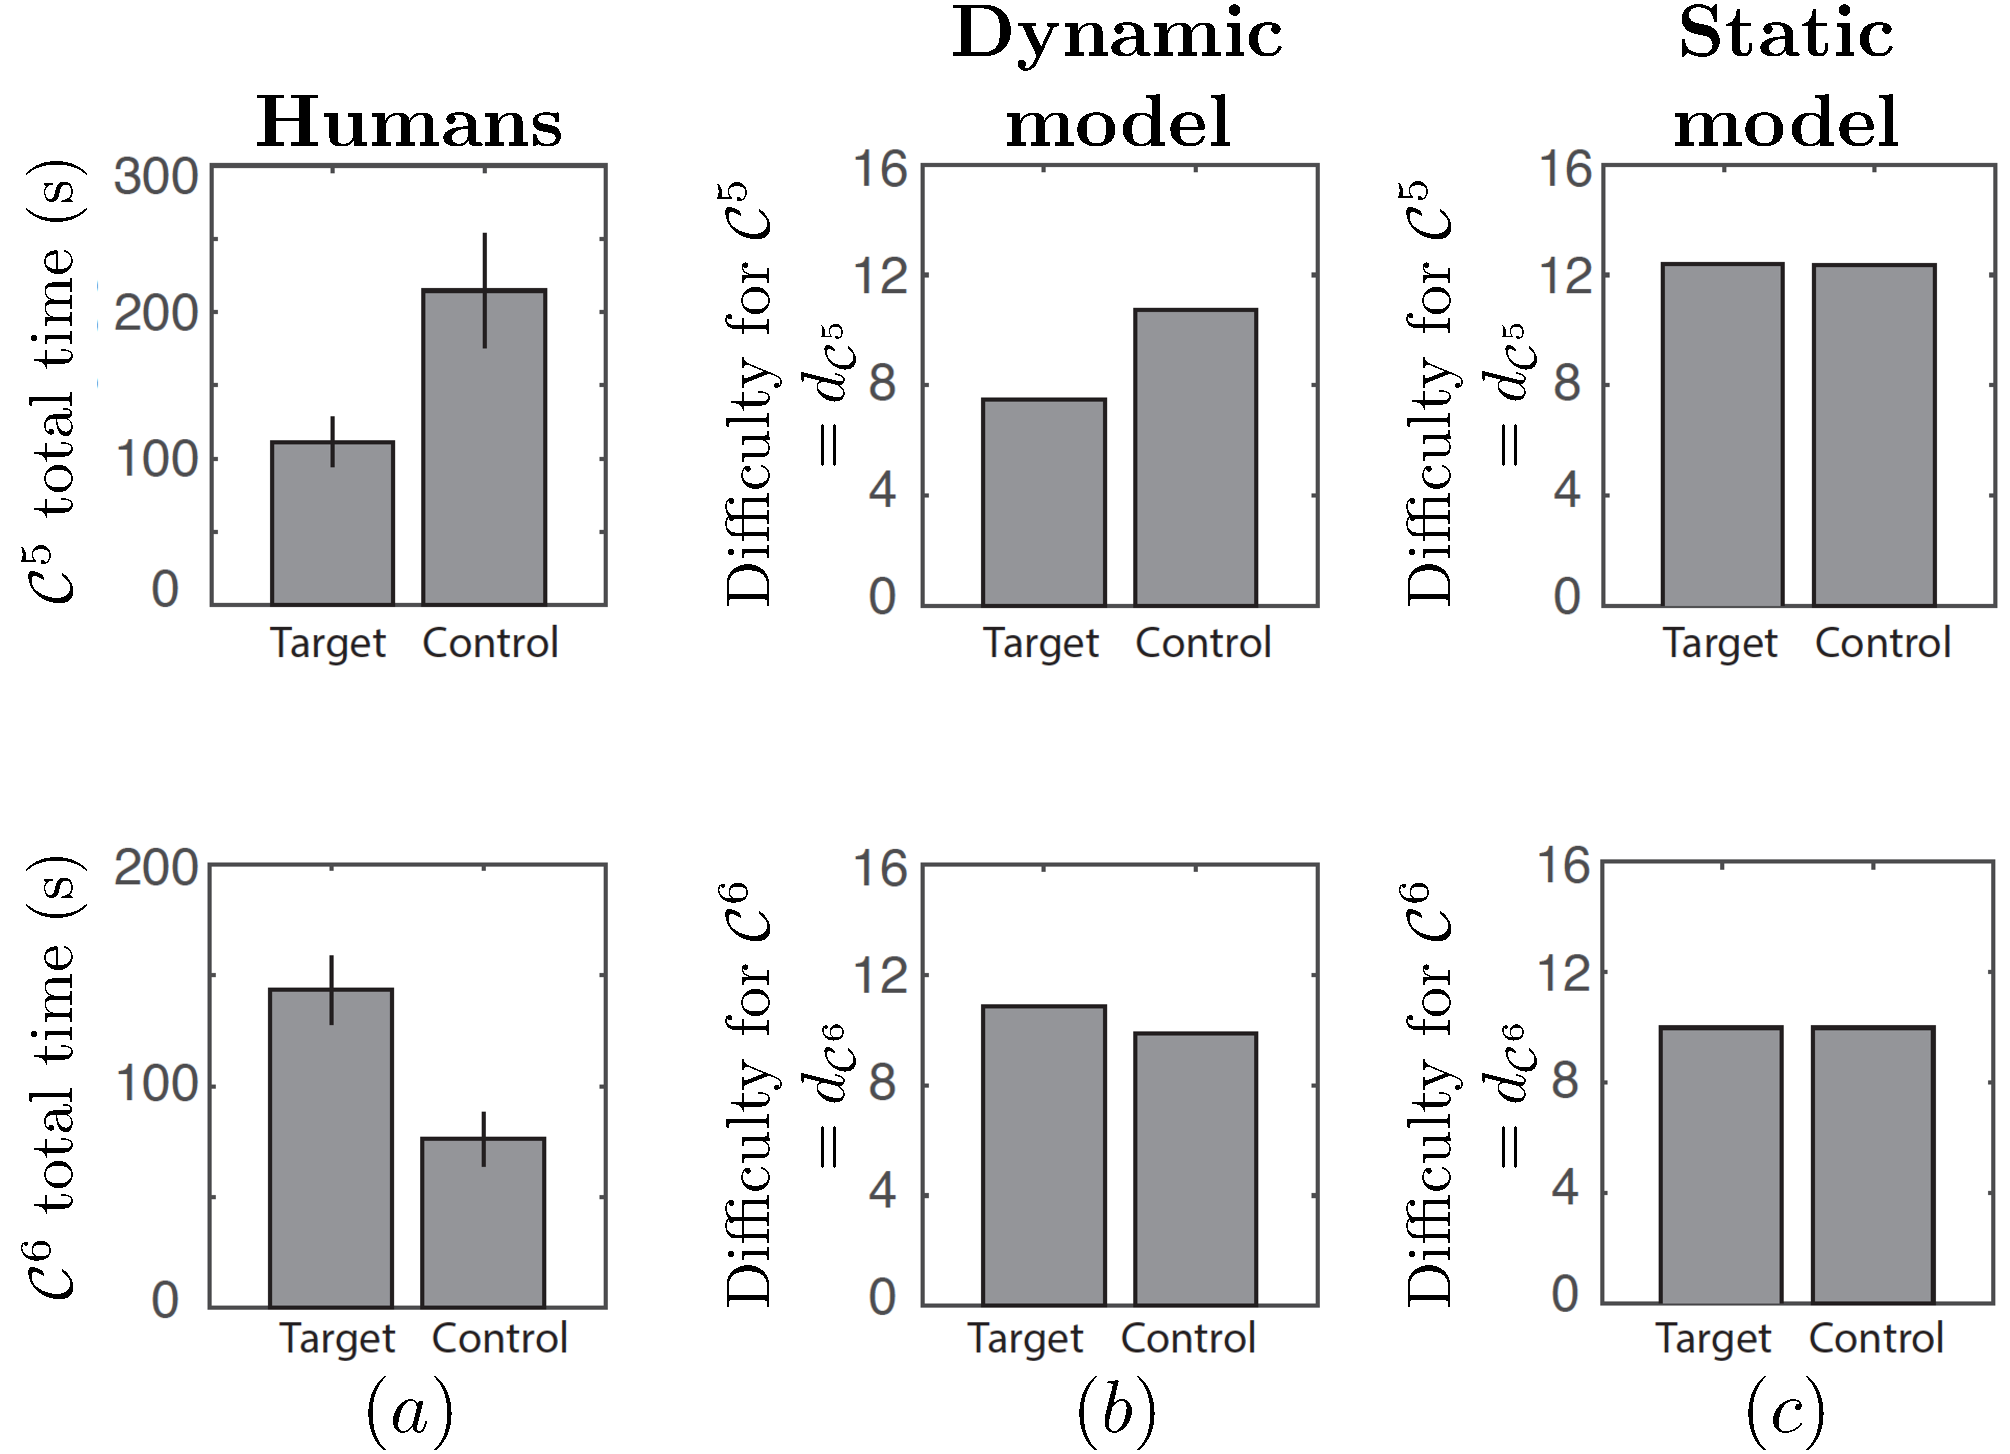
\includegraphics[scale=0.25]{model_free-3.pdf}
      \centering
      \caption{Concept learning time $(a)$ and difficulty predicted $(b)$, $(c)$ for the two test concepts (\testa and \testb). Error bars are s.e.m.\ across subjects.}
      \label{model free}
   \end{figure}
   
\section{Model}

When presented with a concept (e.g.~Fig.~\ref{semaforos}), our model generates logical formulas and evaluate them to true or false for that concept, keeping the formula only if it is true. To generate formulas, the model uses a symbolic language in which each rule (symbols and operators) is associated with a probability of being used. The probability of generating a formula is proportional to the product of the probabilities of the rules required for building it, and therefore it decreases exponentially with its length. Furthermore, if one of the rules has a very low probability of being used, formulas that require it will also have very low probability.

The \textit{Static model} maintains the rules' probabilities fixed throughout the concept sequence (the 6 concepts in Table~\ref{conceptos}). The \textit{Dynamic model} updates the probabilities after each concept, in order to minimize the expected description length of future concepts, assuming they have similar structure to the concepts learnt so far. We include in this model the $\oxor$ rule a priori in the language, but with vanishing probability of being used. Changes in this probability can be analogously interpreted as the probability that a rational agent without the compiled symbol a priori decides to add the compiled expression as a new primitive into her language. %This means that our model will fit somewhere between the computational and the algorithmic level of analysis by Marr's \cite{marr1979computational,griffiths2015rational}. It can explain algorithmically how learning occurs, however, adding a new primitive is not modeled entirely at this level. The vanishing probability analogy is sufficient to make the new primitive be highly unlikely to be used without exposure and to allow it to emerge after concepts. Still, it does not explain --at an algorithmic level-- how any new primitive can arise, leaving the mechanics of the language change between the computational and algorithmic level.


\subsection{Static Model}

\newcommand{\form}{\varphi}
Under the LoT assumption,  given a concept $\con$ (e.g.\ Fig.~\ref{semaforos}), the probability that an agent uses formula $\form$ to explain this concept is defined by Bayes theorem: 
$$
P(\form\mid \con) \propto P(\con\mid \form)P(\form).
\label{Bayes fix}
$$
% \begin{equation}
% P(\form\mid \con) \propto P(\con\mid \form)P(\form).
% \label{Bayes fix}
% \end{equation}
%
The likelihood $P(\con\mid \form)$ of a logical statement $\form$ can be simply defined as 1 if $\sem{\form}=\con$ and 0 otherwise. In other words, for any given concept, only explanations that describe this concept are considered as possible explanations. The likelihood term has been defined more flexibly in the literature~\cite{goodman2008rational,piantadosi2016logical}, allowing for mislabeled elements. We keep this simpler definition in order to reduce the number of free parameters of the model, as we do not intend to account for mislabeling errors in our experiment.

The prior $P(\form)$ is defined by augmenting the context-free grammars shown in Fig.~\ref{PCFG} into a probabilistic context-free grammars (PCFG). In the PCFG, each rule has associated a parameter indicating the probability of using that rule. A PCFG can be used to produce logical statements similar to a CFG. Each non-terminal remaining in the statement is expanded using a rule of the PCFG with probability proportional to that rule's associated parameter, until no non-terminals remain in the statement. 

We assume that the probability that a subject uses formula $\form$ to explain concept $\con$ is proportional to the posterior $P(\form \mid \con)$, and the subjective difficulty $d_\con$ of a concept $\con$ to a participant is proportional to the length of the formula that the participant is using to explain that concept. However, there is no way to know directly which internal formula $\form$ the participant is using (and therefore we do not know $|\form|$). Hence, the most parsimonious approach is to consider the entire posterior distribution $\textbf{P}(\form \mid \con)$ over possible formulas.\footnote{This is equivalent to the Sampling Hypothesis described in~\cite{denison2013rational}, by which participants represent distributions through samples. Similar results are obtained if each participant carries entire probability distributions.}

Given a concept $\con$, the expected length $E_\con$ of the formulas used by the participant is simply
%
 \begin{equation}
E_\con=\sum_{\sem{\form}=\con} |\form| \ P(\form \mid \con),
 \label{expected length}
 \end{equation}
%
where the sum is over all formulas $\varphi$ compatible with $\con$. We  define the difficulty $d_\con$ of a concept experienced by the participant  as $$d_\con \propto E_\con + \alpha N_\con,$$
%
% \begin{equation}
%d_\con \propto E_\con + \alpha N_\con,
% \label{length}
% \end{equation}
%
where we added a term that accounts for the cardinality of the concept: $N_\con$ is the cardinality of the concept or its complement, the one being smaller, i.e.\ $N_\con=\min \{ \#\con, \#\overline \con\}$ (e.g.\ $N_\con=4$ for the concept $\con$ of  Fig.~\ref{semaforos}), and $\alpha$ is a free parameter fitted globally for all concepts and participants to its maximum likelihood value of 0.9. In this way, we remove the asymmetry between positive and negative examples, while accounting for the toil taken by considering a larger number of items simultaneously.

In practice, to approximate $E_\con$ for each concept $\con$, we calculated the posterior probability $P(\form\mid \con)$ of all compatible formulas $\form$s up to size 19 with $P(\form\mid \con)$ and then use ~\eqref{expected length}. Since the space of all possible $\form$s grows exponentially with $|\form|$, normative procedures for estimating $P(\form\mid \con)$ in this space involve stochastic search algorithms. However, in our case, we were able to exhaustively enumerate and calculate the posterior probability of \textit{all} formulas generated by the PCFG up to a sufficiently high size $M$ such that all formulas with $|\form|>M$ have vanishing probabilities when compared to shorter compatible formulas for the current concept (because the prior $P(\form)$ decreases exponentially with the size of the formula).

\subsection{Dynamic Model}

Up to this point, we assumed that, given a concept $\con$, the posterior distribution over formulas $P(\form\mid \con)$ was independent of the other concepts presented in the sequence. However, if the LoT (i.e. the PCFG) updates with experience, the prior $P(\form)$ in $P(\form\mid \con)$ will change, and so will $E_\con$ in \eqref{expected length} and finally the subjective difficulty $d_\con$. Therefore, $d_\con$ will depend on the sequence of concepts that were previously presented to the participant.

In other words, since now $P(\form)$ depends on the sequence of concepts experienced by the participant, instead of $P(\form\mid \con)$, we have $$P(\form\mid \con^{t},\dots,\con^{1}) \propto P(\con^{t}\mid \form)P(\form\mid \con^{1},\dots,\con^{t-1})$$, 
% \begin{equation}
% P(\form\mid \con^{t}) \propto P(\con^{t}\mid \form)P(\form\mid \con^{1},\dots,\con^{t-1}),
% \label{Bayes}
% \end{equation}
%
where $\con^{t}$ is the concept presented at trial~$t$, and $P(\form\mid \con^{1},\dots,\con^{t-1})$ depends on the state of the PCFG at trial $t$, which in turn depends on how the PCFG gets updated from trial to trial.

Intuitively, the update process increases the probability of using a certain rule in the PCFG accordingly to how useful this rule was to compress compatible formulas for the concepts previously learned in the same domain. Specifically, we model the update process in a normative manner: the probability of using a rule of the PCFG at trial $t$ is equal to the Bayesian posterior probability that this rule will enable the learner to find compressed explanations at trial $t$, according to how useful it was to compress explanations in trials $1,\dots,t-1$.

To formalize the update of the PCFG, we define $P(\form)$ similarly to~\cite{goodman2008rational}. Specifically, the prior probability of a logical statement at trial $t$ in the concept sequence uses a single Dirichlet-multinomial for the set of rule expansions. The Dirichlet is parameterized by a set of positive real numbers $D_{i}^{t}$, one for each rule $i$ in the PCFG, which in turn determine the probability of using rule $i$ at trial $t$: a higher $D_{i}$ indicates a higher probability of using rule $i$.

The prior is specified by the set Dirichlet parameters $\textbf{D}^{0}$ with which we start the experiment ($\textbf{D}^{0}$ represents a vector containing the prior parameters of all rules in the grammar at trial 0). In our experiment, we set the prior Dirichlet parameters of all rules equal to 1, and the parameter of the rule that expands the target operator to a value several orders of magnitude smaller ($\approx 10^{-4}$). This means that the target operator was practically absent at the beginning of the experiment, but it was technically possible to `learn it' by increasing its probability as the experiment developed.

Under the Dirichlet model, the prior $P(\form\mid \con^{1},\dots,\con^{t-1})$ can be rewritten using the Dirichlet parameters as $P(\form\mid\textbf{D}^{t})$. Therefore, to know how $P(\form\mid \con)$ updates from trial to trial, we only need to know how $\textbf{D}$ updates from trial to trial.

The Dirichlet parameter of rule $i$ at trial $t+1$ is equal to its parameter at trial $t$ plus the amount of times the production $i$ was used in generating all formulas compatible with the concept at trial $t$ (we note $M_{i}(\form)$ as the number of times that rule $i$ is used in generating formula $\form$), weighted by each formula's posterior probability at trial $t$:
 \begin{equation}
 D_{i}^{t+1}=D_{i}^{t}+\sum_{\sem{\form}=\con^t} P(\form\mid \textbf{D}^{t}) \ M_{i}(\form).
 \label{Dirichlet}
 \end{equation}
 %
This Bayesian learning mechanism increases the probability of using rules that allow concepts to be succinctly described. This happens because these formulas have higher probability $P(\form\mid \textbf{D})$ than longer formulas, so the Dirichlet parameters of the rules that build these formulas increase more strongly than those of the rules that build longer formulas.   

\section{Results}

The Bayesian agent that minimizes the expected complexity of future concepts by optimally adapting its LoT to the inferred structure of the task accurately captures the dynamics of human learning across concepts. If we did not allow the model to update the probability of the operators after each concept, and particularly the compiled operator $\oxor$, the control group and the target group would be indistinguishable to the model as it would predict equal average formula length for both groups (see Fig.~\ref{model free}, {\em Static Model}). Instead, as shown in Fig.~\ref{results}, by adjusting the prior probabilities based on concept exposure the dynamic model is able to capture learning time patterns in the target groups ($R^{2}=0.96$ compared to $R^{2}=0.73$ for the static model). Expectedly, both models perform similarly in the control groups as they were designed to not encourage the use of any particular operator ($R^{2}=0.72$; $R^{2}=0.71$ for the static model). The impact of the learning capability of the model is most evident in the target group concept sequence, which was designed to this effect. If the structure of the concepts does not bias the LoT primitives one way or the other, it is expected that a static model will provide a reasonable fit. However, it is difficult to tell a priori how unbiased a set of concepts really is, so experiments relying on repeated concept exposure should always take between-concept learning into account.

Allowing the model to constantly update its beliefs from concept to concept is a requisite to capture human learning times. We now explain how the pattern of subjective difficulties in Fig.~\ref{results} emerged in the \textit{Dynamic model}. In this scenario, learning for the model is formalized by the update of rule parameters from concept $t$ to concept $t+1$ according to \eqref{Dirichlet}. In Fig.~\ref{evol} we show how this learning takes place in the concept sequence for the target group. There are mainly two competing formulas when \targetb is presented: $x_{i} \oxor x_{j}$ and $(x_{i} \oand \neg x_{j}) \oor (\neg x_{i} \oand x_{j})$. Given the low a priori value of the parameter of the $\oxor$ rule, the posterior of the formulas of type $(x_{i} \oand \neg x_{j}) \oor (\neg x_{i} \oand x_{j})$, which do not use the $\oxor$ operator, is much higher than the posterior of $x_{i} \oxor x_{j}$. Therefore, in Fig.~\ref{results} we see a large predicted difficulty by the dynamic model for this concept (since the posterior lies mainly over these longer formulas without $\oxor$, see  \eqref{expected length}). 

\begin{figure}
      \centering
      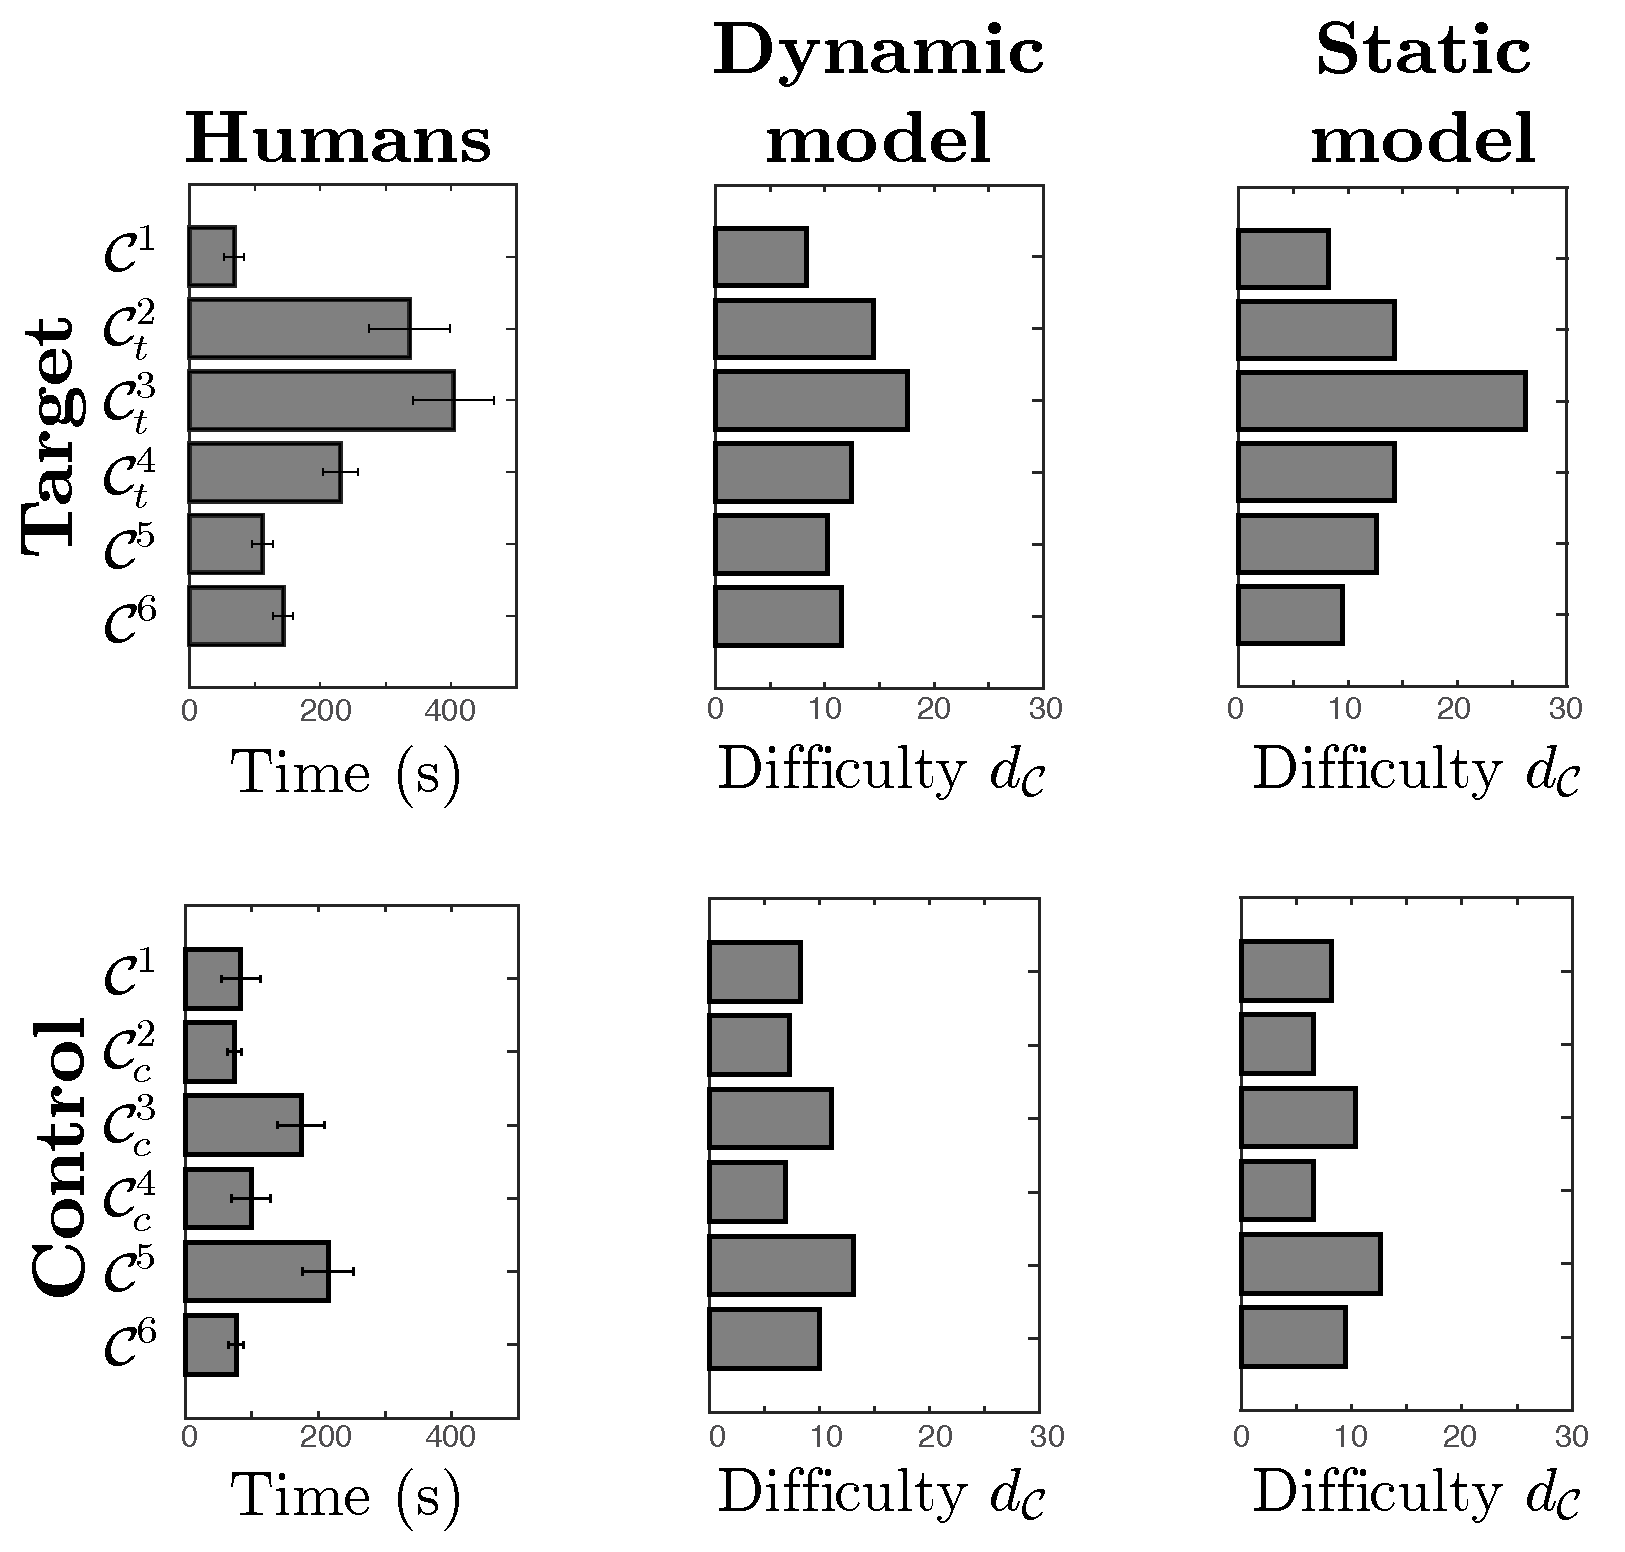
\includegraphics[scale=.30]{results-3.pdf}
      \caption{Learning times and model predictions for target and control groups (see Table~\ref{conceptos} for concept details). The predicted difficulties of each model were calculated using $d_\con$. Error bars are s.e.m.}
      \label{results}
\end{figure}

\begin{figure}
        \centering
        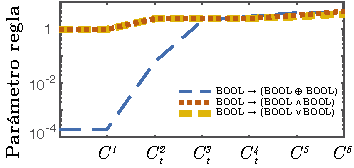
\includegraphics[scale=1]{dirichlet_evol-2.pdf}
        \caption{Evolution of Dirichlet parameters of different rules after each concept experienced by the target group.}
       \label{evol}
\end{figure}\santi{aca hay alguna diferencia de nomenclatura de conceptos. Prefier llamarlos $C^1, C^2$, o lo que sea igual a BRM}


However, the little increment in the $\oxor$ rule after \targetb (see Fig.~\ref{evol}) is sufficient for making the formula $x_{k} \oxor x_{l}$ to have higher relative posterior in the next concepts, making the increment in the parameter of the $\oxor$ rule much greater than before. Additionally, the difficulty inferred by the model is much smaller the second time the concept is presented (compare \targetd and \targetb concepts in Fig.~\ref{results}), since now the posterior is more evenly distributed between long (without $\oxor$) and short (with $\oxor$) formulas (see Eq. \eqref{expected length}). Finally, when the concept \testa is presented, the learner has completely compiled the $\oxor$ rule into her language, ascribing the formulas that use the $\oxor$ operator a much higher posterior probability relative to the long formulas that do not use the $\oxor$ operator. Therefore, the inferred difficulty for \testa is much smaller than those describing previous concepts, almost as simple as concept \targeta (see Fig.~\ref{results}).

Finally, the strong $\oxor$ acquired by the target group increases the difficulty of \testb relative to the control group (see Fig. 3). This occurs because there are several formulas of length 9 that use the $\oxor$ operator (around 6000), significantly increasing the expected difficulty of the concept (see Eq. \eqref{expected length}). For the control group, the posterior probability of these formulas is very low, causing a smaller increase in the expected difficulty.

The previous results point to a competition between different rules in the grammar. In our model, competition between $\oxor$ and the other operators is modulated by the initial relative value of the Dirichlet prior of the $\oxor$ rule, and the overall magnitude of the priors of all rules. The initial $\oxor$ prior measures how useful $\oxor$ should be (relative to the other rules) in order to increase the likelihood of using it in the future. If the $\oxor$ prior is too low relative to the priors of other rules, then formulas with $\oxor$ must be much shorter than formulas without $\oxor$ in order for them to have appreciable posterior and increase the $\oxor$ parameter in Eq. \eqref{Dirichlet}. In our experiment, if the prior is smaller $10^{-12}$ (and 1 for all other rules), then the predictions of the dynamic and static model for the target group are approximately equal: the advantage of using $\oxor$ in the target concepts is not enough to increase the likelihood of using $\oxor$. On the other hand, if the $\oxor$ prior is too high, we cannot model the high difficulty of \targetb for the target group and the high difficulty of \testa for the control group. For example, if the $\oxor$ prior is higher than 0.05 (and 1 for all other rules), the difficulty of \targetb and \targetd are approximately equal (corresponding to the short formula with $\oxor$) and also the difficulties of \testa for control and target groups.

The other free parameter that modulates competition is the overall magnitude of the Dirichlet priors, which determines how many times an efficient rule should be encountered before incorporating it. If the magnitude is too high, then observing a useful rule does not significantly change its Dirichlet parameter relative to the others, eliminating from the model the rapid rule acquisition clearly showed by participants. This happens because in Eq. \eqref{Dirichlet} the magnitude of the updates from $t$ to $t+1$ are at most of order $M$, the number of times that operators appear in formulas with high posterior. In our experiment, if all rules have prior equal to 1 and $\oxor$ has 1/1000 we get similar results to the ones in Fig.~\ref{results}, but if all rules have prior equal to 10000 and $\oxor$ has 10 the additions to the $\oxor$ parameter are insignificant, so the dynamic and static models make the same predictions for the target group.

In our model a large enough exposure to a concepts will increase the Dirichlet parameters without bounds, progressively decreasing learning flexibility. Although our experiment is not long enough to test it, such inflexibility is very unlikely to be true. For example, in the LoT fitting experiment from ~\cite{piantadosi2016logical} they found that human Dirichlet priors for most propositional operators are between 0.3 and 3, instead of orders of magnitude higher (as expected by Eq. \eqref{Dirichlet} after exposure to a large number of concepts). Therefore, a more complete model of lifelong language acquisition should include an extra normalization or forgetting parameter that decreases the overall magnitude of the Dirichlet parameters, preserving the high learning flexibility that we observed in our experiment.


\section{Discussion}

\par We measured the subjective difficulty that participants experience when learning a sequence of concepts. To explain this subjective difficulty, we resource to propositional logic as a  base description language. In the target group we experimented with concepts which can be succinctly described in the base language {\em that also contains an extra operator $\oxor$} for exclusive disjunction but that needed necessarily longer descriptions over the base language (where this operator is absent). On the contrary, the control group is exposed to concepts where $\oxor$ does not help to achieve succinctness.

Learning times are consistent with the hypothesis that participants in the target group smoothly adopt the $\oxor$ as a new primitive of their LoT in order to absorb the concepts they have been exposed to, with no more incentive than decreasing the expected complexity of future concepts. We do not claim that participants have learned the $\oxor$ operator defined by any specific formula using the previous operators, however, their LoT seems to have constructed an operation that matches the semantics of the exclusive or in order to compress such patterns of data and identify them more efficiently.

\par Here, we focus on transfer learning effects when learning sequential concepts that share the same hierarchical structure. We acknowledge, however, that several other transfer learning effects are present in human sequential logical concept learning, such as when subsequent concepts differ in the relevant variables (e.g.\  color lights in our experiment) \cite{blair2009extremely}, when changing the relevant variables in subsequent exclusive disjunctions \cite{kruschke1996dimensional}, or when two categories are learned in an interleaved or a focused manner \cite{carvalho2014putting}. However, unlike superficial knowledge about the task (like the frequency of appearance of different symbols and logical operators in the concept sequence), identifying the latent hierarchical structure of concepts have extremely important computational consequences: it allows for exponentially less complex representations \cite{bengio2013representation,lake2015human}, maximizing the expected value of future computations within resource-bounded constraints~\cite{gershman2015computational}. In our task, in order to focus primarily on the learning process of the $\oxor$ structure, we randomize variables in each trial, such that other kinds of transitions are averaged out across participants. 

\par Most LoT studies provide a language that is fixed once trained or inferred over a specific data. We claim that when a specific language beats a second one at fitting some experimental data, what we may be seeing is an effect of prior experience (including from the experiment itself), more than an intrinsic feature of the LoT. This leads to a fundamental difficulty in trying to experimentally uncover what the actual human symbolic substrate of thought is. Experimental results have shown for instance that a grammar with \textit{and, or}, and \textit{not} better explains Boolean concept learning than one with \textit{nand}, despite both being expressively equivalent~\cite{piantadosi2016logical}.  In our view, this cannot be taken to mean anything more than that in the current state of affairs of the world, the \textit{nand} operator is not very useful for compressing information. We have shown that participants can rapidly compile new expressions in their LoT if they begin to be useful, which emphasizes that one cannot simply ignore the order in which concepts are presented to the participant when studying aspects of the LoT.

When Fodor proposed the Language of Thought hypothesis \cite{fodor1975language}, what he had in mind was a symbolic system we all came equipped with from birth. Stating that this language is in fact always flexible might seem in outright contradiction with Fodor's original idea. In fact, what studies in the LoT literature (including this one) are probably probing is one among many languages in a hierarchy of increasing abstraction. As we progress in life, we find some conceptual summaries useful, and compiled them in a more abstract token. It is even likely that there is no proper hierarchy with sharply defined boundaries between levels, but instead a less organized progression of concepts of increasing abstraction, with thought progressing seamlessly using constructs at different levels. %Further empirical studies of the way we reuse concepts will hopefully pave the way for a broader understanding of human cognition.


\section{Conclusion}

We defined a model to measure the subjective difficulty of learning a sequence of concepts. The model updates the grammar production probabilities between concepts and predicts difficulty as the size of compatible formulas weighted by their posterior probability. This learning mechanism allows to simulate the emergence of a new primitive in the language, as it becomes useful to encode the concepts presented so far. The predicted difficulties strongly resembles the pattern of human learning times in a sequence of concepts that required the $\oxor$ operator in order to be efficiently represented.

    %%!TEX root = ../main.tex


\chapter{Un marco lógico para estudiar aprendizaje de conceptos en presencia de explicaciones múltiples}


\begin{abstract}
% When people seek to understand concepts from an incomplete set of examples and counterexamples, there is usually an exponentially large number of classification rules that can correctly classify the observed data, depending on which features of the examples are used to construct these rules. A mechanistic approximation of human concept-learning should help to explain how humans prefer some rules over others when there are many that can be used to correctly classify the observed data. Here, we exploit the tools of propositional logic to develop an experimental framework that controls the minimal rules that are \textit{simultaneously} consistent with the presented examples. For example, our framework allows us to present participants with concepts consistent with a disjunction \textit{and also} with a conjunction, depending on which features are used to build the rule. Similarly, it allows us to present concepts that are simultaneously consistent with two or more rules of different complexity and using different features. Importantly, our framework fully controls which minimal rules compete to explain the examples and is able to recover the features used by the participant to build the classification rule, without relying on supplementary attention-tracking mechanisms (e.g.\ eye-tracking). We exploit our framework in an experiment with a sequence of such competitive trials, illustrating the emergence of various transfer effects that bias participants' prior attention to specific sets of features during learning.
Cuando las personas buscan comprender conceptos a partir de un conjunto incompleto de ejemplos y contraejemplos, suele haber una cantidad exponencial de reglas de clasificación que pueden clasificar correctamente los datos observados, según las características de los ejemplos que se utilicen para construir estas reglas. Una aproximación mecanicista del aprendizaje de conceptos humanos debería ayudar a explicar cómo los humanos prefieren algunas reglas por sobre otras cuando hay muchas que pueden usarse para clasificar correctamente los datos observados. Aquí, explotamos las herramientas de la lógica proposicional para desarrollar un marco experimental que controle las reglas mínimas que son \textit{simultáneamente} consistentes con los ejemplos presentados. Por ejemplo, nuestro marco nos permite presentar a los participantes conceptos consistentes con una disyunción \textit{y también} con una conjunción, dependiendo de qué características se usen para construir la regla. Del mismo modo, nos permite presentar conceptos que son simultáneamente consistentes con dos o más reglas de diferente complejidad y que utilizan diferentes características. Es importante destacar que nuestro marco controla completamente qué reglas mínimas compiten para explicar los ejemplos y es capaz de recuperar las características utilizadas por el participante para construir la regla de clasificación, sin depender de mecanismos complementarios de seguimiento de la atención (por ejemplo, {\em eye-tracking}). Explotamos nuestro marco en un experimento con una secuencia pruebas competitivas como las mencionadas, e ilustramos la aparición de varios efectos de transferencia que sesgan la atención previa de los participantes a conjuntos específicos de características durante el aprendizaje.
\end{abstract}



% Concept acquisition is a key and widely studied aspect of human daily cognition \cite{cohen2005handbook, ashby2011human}. Many researchers have claimed that a coding system and a set of rules underlie some of our  abilities to acquire concepts \cite{nosofsky1994rule,tenenbaum2011grow,maddox1993comparing}, and it has been observed that we seem to learn concepts of objects with more ease when there are `simpler' rules that can explain those groupings \cite{shepard1961learning, nosofsky1994comparing, rehder2005eyetracking, lewandowsky2011working,feldman2000minimization,blair2003easy,minda2001prototypes}. 
La adquisición de conceptos es un aspecto clave y ampliamente estudiado de la cognición diaria humana \cite{cohen2005handbook, ashby2011human}. Muchos investigadores han afirmado que un sistema de codificación y un conjunto de reglas subyacen a algunas de nuestras habilidades para adquirir conceptos \cite{nosofsky1994rule, tenenbaum2011grow, maddox1993comparing}, y se ha observado que parece que aprendemos conceptos de objetos con más facilidad cuando hay reglas `más simples' que pueden explicar esas agrupaciones \cite{shepard1961learning, nosofsky1994comparing, rehder2005eyetracking, lewandowsky2011working, feldman2000minimization, blair2003easy, minda2001prototypes}.

% In the real-world, humans learn concept descriptions while simultaneously deciding on which features to attend \cite{schyns1998development}; and the selected set of features usually determines the structure and complexity of the minimal rules that can describe the concept. For example, the concept \textit{dog} can be explained as {\em a four-legged pet that is not a cat} or as {\em an animal for hunting, herding, pulling sledges or company}. Both descriptions are fully compatible with the concept \textit{dog}, but our experience induces us to choose different relevant features to define the concept. While the first description of {\em dog} could be very well be given by a child having a dog at home, the second could be given by a shepherd or perhaps an ethologist. It is likely that the features used to describe {\em dog} by each agent allows them to compactly describe the concept, while simultaneously separating it from other concepts frequently encountered in their environment. Here, we ask about which features participants use to describe concepts, depending on the logical structure of the description using those features and also on their exposure to previous concepts. Why will someone use {\em cat} or {\em hunting} to define {\em dog}?
En el mundo real, los humanos aprenden descripciones de conceptos mientras deciden simultáneamente a qué características atender \cite{schyns1998development}; y el conjunto de características seleccionado generalmente determina la estructura y complejidad de las reglas mínimas que pueden describir el concepto. Por ejemplo, el concepto \textit{perro} se puede explicar como {\em una mascota de cuatro patas que no es un gato} o como {\em un animal para caza, pastoreo, tira de trineos o compañía}. Ambas descripciones son totalmente compatibles con el concepto \textit{perro}, pero nuestra experiencia nos induce a elegir diferentes características relevantes para definir el concepto. Mientras que la primera descripción de {\em perro} podría muy bien haber sido dada por un niño que tiene un perro en casa, la segunda podría haber sido presentada por un pastor o quizás un etólogo. Es probable que las características utilizadas para describir {\em perro} por cada agente les permitan describir de manera compacta el concepto, al mismo tiempo que lo separan de otros conceptos que se encuentran con frecuencia en su entorno. Aquí, preguntamos qué características usan los participantes para describir conceptos, dependiendo de la estructura lógica de la descripción que usa esas características y también de su exposición a conceptos anteriores. ¿Por qué alguien usaría {\em gato} o {\em caza} para definir {\em perro}?
\begin{figure}
\begin{center}
% 	\includegraphics[scale=.6]{papers/images_behavior_research_methods/intro_notation.pdf}
% \end{center}\caption{Illustration of the features $\{p_1,p_2,p_3,p_4\}$, the example $(1,1,0,1)$, and a concept (positive example are marked with bold boundaries and negative examples with thin boundaries). The concept can be explained with the two minimal rules $p_1 \land p_2$ or $p_3 \lor p_4$, depending on which features are used to build the rule (the first two features or the last two features, respectively).}
	\includegraphics[scale=.6]{papers/images_behavior_research_methods/intro_notation_sp.pdf}
\end{center}\caption{Ilustración de las características $\{p_1,p_2,p_3,p_4\}$, el ejemplo $(1,1,0,1)$, y un concepto (los ejemplos positivos están marcados con marcos gruesos y los ejemplos negativos con marcos delgados). El concepto se puede explicar con las dos reglas mínimas $p_1 \land p_2$ o $ p_3 \lor p_4$, dependiendo de las características que se usen para construir la regla (las dos primeras características o las dos últimas características, respectivamente).}
\label{fig:intro_notation}
\end{figure}



% In propositional concept-learning experiments, participants are presented with a set of \textit{examples}, each conformed of $N$ propositional \textit{features}, which can take positive or negative values. For instance, for $N=4$ one example can be logically represented as the element $(1,1,0,1)$, which takes positive values for the first, second and fourth features and negative for the second one, as illustrated in Figure~\ref{fig:intro_notation}. A \textit{concept} can be intuitively understood as a set of examples, some of them marked as belonging to the concept and the rest marked as not belonging, i.e.\ positive and negative examples. In Figure~\ref{fig:intro_notation} we show an example of an \textit{underdetermined} concept, in the sense that, since the entire universe of examples is not shown (i.e. the $2^4$ possibilities), different determined concepts can be consistent with this smaller set when extending the set of examples to the full universe. 
En los experimentos de aprendizaje de conceptos proposicionales, a los participantes se les presenta un conjunto de \textit{ejemplos}, cada uno conformado por $N$ \textit{features} proposicionales, que pueden tomar valores positivos o negativos. Por ejemplo, para $N=4$ un ejemplo se puede representar lógicamente como el elemento $(1,1,0,1)$, que toma valores positivos para la primera, segunda y cuarta características y negativos para la segunda, como ilustramos en la Figura ~\ref{fig:intro_notation}. Un \textit{concepto} puede entenderse intuitivamente como un conjunto de ejemplos, algunos de ellos marcados como pertenecientes al concepto y el resto marcados como no pertenecientes, es decir, ejemplos positivos y negativos. En la Figura~\ref{fig:intro_notation} mostramos un ejemplo de un concepto \textit{subdeterminado}, en el sentido de que, dado que no se muestra universo completo de ejemplos (es decir, las $2^4$ posibilidades), diferentes conceptos determinados pueden ser coherentes con este conjunto más pequeño al extender el conjunto de ejemplos al universo completo.


% A \textit{rule} consistent with the concept is a logical formula built with the features and the conjunction ($\land$), disjunction ($\lor$), and negation ($\lnot$) operators, which evaluates to true for objects belonging to the concept and false otherwise (e.g.\ $p_1 \land p_2$, where $p_i$ is the $i^{th}$ feature, see Figure~\ref{fig:intro_notation}). The \textit{minimal description length} (\textit{MDL}) of a concept is the length of the shortest rule consistent with the concept \cite{grunwald2007minimum} (here, the {\em length} of a formula is defined as the number of positive or negative occurrences of propositional symbols plus the number of occurrences of operators $\land$ or $\lor$ contained in it; for example, the length of $p_1 \land \lnot p_3$ is 3, and the length of $(p_1 \land \lnot p_3)\lor p_2$ is 5). Importantly, most studies of subjective difficulty with concept-learning are designed such that a {\em single} minimal rule can be used to describe the concept (e.g.\ $p_1 \land p_2$) \cite{ashby2005human,feldman2000minimization}, even when the difficulty of finding the features that compose that rule ($p_1$ and $p_2$) is measured with attention-tracking mechanisms (e.g.\ \cite{blair2009extremely,hoffman2010costs}). This limitation is possibly due to the prohibitively large number of rules that can be built with a given set of features, making it difficult to control which rules the participant might use when observing a set of examples. For instance, in order to determine the difficulty that participants have in learning the logical rule $p_1 \lor p_2$, it is crucial to control that no other rule of reasonable complexity can explain the concept (e.g.\ $p_1 \land p_3$). In this work, we use the tools of propositional logic to build an experimental framework that allows us to present examples consistent with two (or more) chosen rules, depending on which features are observed. For instance, the concept shown in Figure~\ref{fig:intro_notation} is consistent with the explanation $p_1 \land p_2$ \textit{and also} with the explanation $p_3 \lor p_4$, depending on which features are observed. In general, the experimenter can choose any pair of rules that use any number of (non-overlapping) features, and our framework guarantees that the presented examples are only consistent with the two minimal rules chosen by the experimenter. Then, by presenting novel examples that are consistent with only one of the previous rules, the experimenter can determine which rule the participants internally used to learn the concept, and thus which features they attended to.
Una \textit{regla} consistente con el concepto es una fórmula lógica construida con las características y los operadores de conjunción ($\land$), disyunción ($\lor$) y negación ($\lnot$), que se evalúa como verdadera para objetos que pertenecen al concepto y falsa en caso contrario (por ejemplo, $p_1 \land p_2$, donde $p_i$ es la $i$-ésima característica, ver Figura~\ref{fig:intro_notation}). La \textit{longitud mínima de descripción} (\textit{MDL} por sus siglas en inglés) de un concepto es la longitud de la regla más corta consistente con el concepto \cite{grunwald2007minimum} (aquí, la {\em longitud} de una fórmula se define como número de apariciones positivos o negativos de símbolos proposicionales, más el número de apariciones de los operadores $\land$ o $\lor$ contenidos en él; por ejemplo, la longitud de $p_1 \land \lnot p_3 $ es 3, y la longitud de $(p_1 \land \lnot p_3) \lor p_2$ es 5). Es importante destacar que la mayoría de los estudios sobre la dificultad subjetiva en el aprendizaje de conceptos están diseñados de manera que se pueda usar una {\em única} regla mínima para describir el concepto (por ejemplo, $p_1 \land p_2$) \cite{ashby2005human,feldman2000minimization}, incluso cuando la dificultad de encontrar las características que componen esa regla ($p_1$ y $p_2$) se mide con mecanismos de seguimiento de atención (por ejemplo, \cite {blair2009extremely, hoffman2010costs}). Esta limitación se debe posiblemente a la cantidad prohibitivamente grande de reglas que se pueden construir con un conjunto de características dado, lo que dificulta el control de las reglas que el participante podría usar al observar un conjunto de ejemplos. Por caso, para determinar la dificultad que tienen los participantes en aprender la regla lógica $p_1 \lor p_2$, es crucial controlar que ninguna otra regla de complejidad razonable pueda explicar el concepto (por ejemplo, $p_1 \land p_3$). En este trabajo, utilizamos las herramientas de la lógica proposicional para construir un marco experimental que nos permita presentar ejemplos consistentes con dos (o más) reglas elegidas, dependiendo de qué características se observen. Por ejemplo, el concepto mostrado en la Figura~\ref{fig:intro_notation} es consistente con la explicación $p_1 \land p_2$ \textit {y también} con la explicación $p_3 \lor p_4$, dependiendo de qué características se observen. En general, el experimentador puede elegir cualquier par de reglas que usen cualquier número de características (no superpuestas), y nuestro marco garantiza que los ejemplos presentados solo son consistentes con las dos reglas mínimas elegidas por el experimentador. Luego, al presentar ejemplos novedosos que sean consistentes con solo una de las reglas anteriores, el experimentador puede determinar qué regla usaron los participantes internamente para aprender el concepto y, por lo tanto, a qué características atendieron.


% Presenting rules $A$ and $B$ (e.g.\ $p_1 \land p_2$ and $p_3 \lor p_4$) using the same set of examples has several experimental advantages over separately presenting a set of examples consistent with rule $A$ and then a set of examples consistent with rule $B$. Some of the advantages are: 
Presentar las reglas $A$ y $B$ (por ejemplo, $p_1\land p_2$ y $p_3 \lor p_4$) utilizando el mismo conjunto de ejemplos tiene varias ventajas experimentales sobre la presentación por separado de un conjunto de ejemplos coherentes con la regla $A$ y luego un conjunto de ejemplos consistentes con la regla $B$. Algunas de las ventajas son:

\begin{enumerate}
\item [(1)] 
% When comparing the relative difficulty of learning $A$ and $B$ in the same participant, presenting the examples separately makes it hard to overcome transfer effects that cause subjective difficulty to depend on the history of concepts learnt previously in the task, and cause different relative difficulties if $A$ is learnt before $B$ compared to $B$ being learnt before $A$ (see for example \cite{tano2020towards}). The experimenter could compare learning times for $A$ and $B$ across participants, but for reasonably hard rules there are very large idiosyncratic differences in learning difficulties which greatly increases the variance of learning times (see for example \cite{feldman2000minimization}), and also the experimenter cannot normalize the past history of each participant before the experiment. On the other hand, presenting $A$ and $B$ simultaneously via the same set of examples allows us to directly measure which of the two rules is most easily found by the participant, when the two are presented under exactly the same experimental conditions.
Cuando comparamos la dificultad relativa de aprender $A$ y $B$ en el mismo participante, si presentamos los ejemplos por separado, se complica superar los efectos de transferencia que hacen que la dificultad subjetiva dependa de la historia de conceptos aprendidos previamente en la tarea, y provoquen diferentes dificultades relativas si $A$ se aprende antes de $B$ en comparación a si $B$ se aprende antes de $A$ (ver por ejemplo \cite{tano2020towards}). El experimentador podría comparar los tiempos de aprendizaje para $A$ y $B$ entre los participantes, pero para reglas razonablemente estrictas, existen diferencias idiosincrásicas muy grandes en las dificultades de aprendizaje que aumentan enormemente la variación de los tiempos de aprendizaje (ver, por ejemplo, \cite{feldman2000minimization}). Además, el experimentador no puede normalizar la historia pasada de cada participante antes del experimento. Por otro lado, presentar $A$ y $B$ simultáneamente a través del mismo conjunto de ejemplos nos permite medir directamente cuál de las dos reglas encuentra más fácilmente el participante, cuando las dos se presentan exactamente bajo las mismas condiciones experimentales.

\item [(2)] 
% The fact that rule $A$ is learnt more easily than $B$ when presented separately does not necessarily mean that the same happens when presented jointly. This could not hold if there is an interaction between the logical operators being learnt (that compose the rules $A$ and $B$) and the search mechanism used to find the corresponding rules. For instance, the search mechanism that allows humans to find a disjunction rule consistent with the examples could interact with the mechanism that allows to find conjunctions, an interaction that could only be characterized when the conjunction and disjunction are presented at the same time.
El hecho de que la regla $A$ se aprenda más fácilmente que $B$ cuando se presentan por separado no significa necesariamente que suceda lo mismo cuando se presenta en conjunto. Esto no podría ser válido si existiera una interacción entre los operadores lógicos que se están aprendiendo (que componen las reglas $A$ y $B$) y el mecanismo de búsqueda utilizado para encontrar las reglas correspondientes. Por ejemplo, el mecanismo de búsqueda que permite a los humanos encontrar una regla de disyunción consistente con los ejemplos podría interactuar con el mecanismo que permite encontrar conjunciones, interacción que solo podría caracterizarse cuando la conjunción y la disyunción se presentan al mismo tiempo.

\item [(3)] 
% Our framework allows us to test second-order subjective difficulty effects (e.g.\ rule $A$ is learnt faster if presented jointly with rule $B$ than with rule $C$), as well as second-order transfer learning effects (e.g.\  participants learn more rapidly rule $C$ if they have first observed rule $A$ jointly presented with an arbitrary rule $B_1$, compared to $A$ coupled with a different rule $B_2$).
Nuestro marco nos permite probar efectos de dificultad subjetiva de segundo orden (por ejemplo, la regla $A$ se aprende más rápido si se presenta junto con la regla $B$ que si se presenta junto con la regla $C$), así como efectos de aprendizaje de transferencia de segundo orden (por ejemplo, los participantes aprenden más rápidamente la regla $C$ si primero han observado la regla $A$ presentada conjuntamente con una regla arbitraria $B_1$, en comparación con $ $ junto con una regla diferente $B_2$).

\item [(4)] 
% If one is interested in which features are preferentially observed by the participant in a given trial (e.g.\  features $\{p_1,p_2\}$ or $\{p_3,p_4\}$), one could simply choose the same logical structure for $A$ and $B$ (e.g.\ making $A$ and $B$ equal to $p_1 \land p_2$ and $p_3 \land p_4$) and test whether $A$ or $B$ is learnt by the participant. Then, any preference for learning $A$ over $B$ could only be due to a preference over the features themselves ($\{p_1,p_2\}$), and not for the logical description of the concept using those features (this is, $\boldsymbol{\cdot} \land \boldsymbol{\cdot}$).
Si uno está interesado en qué características observa preferentemente el participante en una prueba determinada (por ejemplo, las características $\{p_1, p_2 \}$ o $\{p_3, p_4 \} $), simplemente se podría elegir la misma estructura lógica por $A$ y $B$ (por ejemplo, haciendo que $A$ y $B$ sean iguales a $p_1 \land p_2$ y $p_3 \land p_4 $) y comprobar si el participante aprende $A$ o $B$ . Entonces, cualquier preferencia por aprender $A$ sobre $B$ solo podría deberse a una preferencia sobre las características en sí mismas ($\{p_1, p_2 \} $), y no por la descripción lógica del concepto que usa esas características (esto es, $\boldsymbol{\cdot} \land \boldsymbol{\cdot}$).
\end{enumerate}



% We illustrate these advantages in an experiment in which participants are presented with a sequence of 6 trials, observing in each trial a set of examples consistent with two alternative rules. We illustrate advantage (1) and (2) discussed above by presenting a conjunction together with a disjunction; and a simple rule together with a complex rule. Then, we show that after observing in several trials that a subset of features is useful to find concise rules, we induce  in the participants a bias to preferentially describe concepts using those features; this bias was tested exploiting  advantage (4).
Ilustramos estas ventajas en un experimento en el que a los participantes se les presenta una secuencia de 6 pruebas, observando en cada prueba un conjunto de ejemplos consistentes con dos reglas alternativas. Ilustramos la ventaja (1) y (2) discutida anteriormente presentando una conjunción junto con una disyunción; y una regla simple junto con una regla compleja. Luego, mostramos que después de observar en varias pruebas que un subconjunto de características es útil para encontrar reglas concisas, inducimos en los participantes un sesgo para describir conceptos usando preferentemente esas características; este sesgo se probó aprovechando la ventaja (4).





%!TEX root = Main.tex

\section{Experimento}\label{Section:Experiment}

\subsection{Participantes} \label{Participants}

% The experiment was conducted as a Human Intelligence Task (HIT) in Amazon's Mechanical Turk \cite{crump2013evaluating, buhrmester2011amazon, stewart2015average}. There were 100 participants,  self-selected workers that saw, accepted, and finished the published HIT. We required workers to have a HIT approval rate of $95\%$ or more. Workers were informed that the payment for completing the experiment was going to be of {1.5} US dollars, and that 1 out of 20 participants would be randomly assigned a bonus of 10 dollars, regardless of their performance in the experiment's tasks as long as they finished the experiment (but note that trials did not end until they correctly learned each concept).
El experimento se llevó a cabo como una tarea de Human Intelligence Task (HIT) en Mechanical Turk \cite{crump2013evaluating, buhrmester2011amazon, stewart2015average} de Amazon. Hubo 100 participantes, trabajadores autoseleccionados que vieron, aceptaron y terminaron el HIT publicado. Requerimos que los trabajadores tuvieran una tasa de aprobación HIT de $95 \%$ o más. Se informó a los trabajadores que el pago por completar el experimento sería de {1,5} dólares estadounidenses,
y que a 1 de cada 20 participantes se le asignaría aleatoriamente una bonificación de 10 dólares, independientemente de su desempeño en las tareas del experimento, siempre que terminaran el experimento (pero tener en cuenta que las pruebas no terminaron hasta que aprendieron correctamente cada concepto).

% For exclusion criteria, see the appendix~\S\ref{Sec:ExclusionCriteria}.
Para conocer los criterios de exclusión, consultar el apéndice~\S\ref{Sec:ExclusionCriteria}.


\subsection{Configuración del experimento}\label{Subsec:ExperimentFlow}
% The main idea of our experimental framework is schematized in Figure~\ref{fig:twoconcepts}. The participants observe an \textit{underdetermined} concept. This concept is presented to the participants as a set of elements that belong to it (positive examples), and a set of elements that do not (negative examples). In  Figure~\ref{fig:twoconcepts}, the elements marked as positive examples are the ones in the intersection of the two concepts and the negative examples are the ones outside of both concepts. Importantly, the listing is incomplete, in the sense that not all elements of the universe are shown. The critical insight is that, when extending the set of examples to the full universe, there is more than one possible concept that is consistent with the observed examples.  For example, in Figure~\ref{fig:twoconcepts},  the presented examples are consistent with the minimal rule of $C_1$ (i.e.\ $\varphi_1=p_1\lor p_2$) \textit{and also} with the minimal rule of $C_2$ (i.e.\ $\varphi_2=p_3\land p_4$). As we explain in the rest of this section, choosing $C_1$ and $C_2$ appropriately can be exploited to control the minimal rules that are consistent with the examples that participants observe.
La idea principal de nuestro marco experimental se esquematiza en la Figura~\ref{fig:twoconcepts}. Los participantes observan un concepto \textit{indeterminado}. Este concepto se presenta a los participantes como un conjunto de elementos que le pertenecen (ejemplos positivos), y un conjunto de elementos que no (ejemplos negativos). En la Figura~\ref{fig:twoconcepts}, los elementos marcados como ejemplos positivos son los que están en la intersección de los dos conceptos y los ejemplos negativos son los que están fuera de ambos conceptos. Es importante destacar que la lista es incompleta, en el sentido de que no se muestran todos los elementos del universo. La idea fundamental es que, al extender el conjunto de ejemplos al universo completo, hay más de un concepto posible que es consistente con los ejemplos observados. Por ejemplo, en la Figura~\ref{fig:twoconcepts}, los ejemplos presentados son consistentes con la regla mínima de $C_1$ (es decir, $\varphi_1 = p_1 \lor p_2$) \textit {y también} con la regla mínima de $C_2$ (es decir, $\varphi_2 = p_3 \land p_4$). Como explicamos en el resto de esta sección, la elección adecuada de $C_1$ y $C_2$ puede aprovecharse para controlar las reglas mínimas que son consistentes con los ejemplos que observan los participantes.


\begin{figure}
\begin{center}
	\includegraphics[scale=.65]{papers/images_behavior_research_methods/twoconcepts3.pdf}
\end{center}\caption{
%An example of a pair of concepts $C_1$ and $C_2$ with 6 features. Concept $C_1$ can be described by $\varphi_1=p_1 \lor p_2$, and $C_2$ by $\varphi_2=p_3\land p_4$. This is just a schematic illustration of where each element (tuple) is placed with respect to concepts. These concepts correspond to the ones used in Trial 1 of the actual experiment. However, elements in the actual experiment are not represented in this way (i.e.\ as tuples of zeroes and ones).
Un ejemplo de un par de conceptos $C_1$ y $C_2$ con 6 características. El concepto $C_1$ puede ser descrito por $\varphi_1 = p_1 \lor p_2 $, y $C_2$ por $\varphi_2 = p_3 \land p_4$. Esta es solo una ilustración esquemática de dónde se coloca cada elemento (tupla) con respecto a los conceptos. Estos conceptos corresponden a los utilizados en la Prueba 1 del experimento real. Sin embargo, los elementos del experimento real no se representan de esta manera (es decir, como tuplas de ceros y unos).
}
\label{fig:twoconcepts}
\end{figure} 

% The actual experiment that we implemented consists of a sequence of 6 trials constructed in this manner. We now expand the 3 stages that compose each $i$-th trial of the experiment. For a better understanding, see Figure~\ref{fig:trials}, which consists of a schematic view of one trial. Note that this figure is merely illustrative and does not aim to describe the details of a trial, but rather the sequence of phases and the logical flow within a trial. In particular, note that the number of elements {\sf A}'s, {\sf B}'s, {\sf C}'s and {\sf D}'s in the figure are not meaningful, as they vary from trial to trial along the experiment. The actual concepts used in each trial, as well as the number of positive and negative examples is listed in Table~\ref{trial_table} (groups X,Y are only relevant for Hypothesis III, so they can be ignored for now), and more details of the actual implementation can be found in \S\ref{sub:experimentdetails} and \S\ref{FullExperimentDescription}.
El experimento real que implementamos consiste en una secuencia de 6 pruebas, cada una de las cuales está construida de esta manera. Ahora expandimos las 3 etapas que componen la $i$-ésima prueba del experimento. Para una mejor comprensión, consultar la Figura~\ref{fig:trials}, que consiste en una vista esquemática de una prueba. Tenga en cuenta que esta figura es meramente ilustrativa y no pretende describir los detalles de una prueba, sino más bien la secuencia de fases y el flujo lógico dentro de una prueba. En particular, tener en cuenta que el número de elementos {\sf A}, {\sf B}, {\sf C} y {\sf D} en la figura no son significativos, ya que varían de prueba en prueba a lo largo del experimento. Los conceptos reales utilizados en cada ensayo, así como el número de ejemplos positivos y negativos se enumeran en la Tabla~\ref{trial_table} (los grupos X, Y solo son relevantes para la Hipótesis \ref{Hip:FeatureBiasTimeAdvantage}, por lo que pueden ignorarse por ahora), y se pueden encontrar más detalles de la implementación real en \S\ref{sub:experimentdetails} y \S\ref{FullExperimentDescription}.  
 \begin{figure}[t]
\begin{center}
	\includegraphics[scale=.7]{papers/images_behavior_research_methods/experimentscheme2_sp.pdf}
\end{center}\caption{
% The scheme of our experimental framework for studying concept learning in the presence of multiple explanations. We illustrate the three phases that constitute each trial: learning phase, training-feedback phase and generalization phase. Elements are represented with letters {\sf A}, {\sf B}, {\sf C} and {\sf D} (for example, the four letters {\sf A} in the intersection represent four different elements in the intersection). The depicted number of such letters {\sf A}, {\sf B}, {\sf C} or {\sf D} is irrelevant (for example, there would be 12 {\sf A}s and 4 {\sf D}s for concepts of Figure~\ref{fig:twoconcepts}).
El esquema de nuestro marco experimental para estudiar el aprendizaje de conceptos en presencia de múltiples explicaciones. Ilustramos las tres fases que constituyen cada ensayo: fase de aprendizaje, fase de formación-{\em feedback} y fase de generalización. Los elementos se representan con las letras {\sf A}, {\sf B}, {\sf C} y {\sf D} (por ejemplo, las cuatro letras {\sf A} en la intersección representan cuatro elementos diferentes en la intersección). El número representado de tales letras {\sf A}, {\sf B}, {\sf C} o {\sf D} es irrelevante (por ejemplo, habría 12 {\sf A}s y 4 {\sf D}s para los conceptos de la Figura~\ref{fig:twoconcepts}).
  }
\label{fig:trials}
\end{figure}

\begin{enumerate}
    % \item \label{item:LearningStage}{\bf Learning stage.} The participant is exposed to a set of `in' elements corresponding to $C^i_1\cap C^i_2$ (marked as `{\sf A}' in Figure~\ref{fig:trials}), and a set of `out' elements corresponding to the {\em complement} of $C^i_1\cup C^i_2$ (marked as `{\sf B}' in Figure~\ref{fig:trials}). 
    \item \label{item:LearningStage}{\bf Etapa de aprendizaje.} El participante se expone a un conjunto de elementos `adentro' correspondientes a $ C^i_1\cap C^i_2$ (marcados como `{\ sf A}' en la Figura~\ref{fig:trials}), y un conjunto de Elementos `afuera' correspondientes al {\em complemento} de $C^i_1\cup C^i_2$ (marcados como` {\sf B}' en la Figura~ ref{fig:trials}).

    
    % We call these shown elements `positive examples' and `negative examples', respectively. Note that this information is incomplete, in the sense that not all possible examples are shown to the participant (as the only examples that are shown from $C^i_1\cup C^i_2$ are those in $C^i_1\cap C^i_2$). In the illustrative example of Figure~\ref{fig:twoconcepts} (corresponding to concepts of Trial 1 of the actual experiment), 24 elements would be shown: the 12 positive examples in the intersection of $C_1$ and $C_2$, and the 12 negative examples outside of both $C_1$ and $C_2$. The participant is asked to learn the concept represented by positive examples.
	A estos elementos mostrados los llamamos `ejemplos positivos' y `ejemplos negativos', respectivamente. Hay que tener en cuenta que esta información es incompleta, en el sentido de que no todos los ejemplos posibles se muestran al participante (ya que los únicos ejemplos que se muestran de $C^i_1 \cup C^i_2$ son los de $C^i_1 \cap C^i_2$). En el ejemplo ilustrativo de la Figura~\ref{fig:twoconcepts} (correspondiente a los conceptos de la Prueba 1 del experimento real), se mostrarían 24 elementos: los 12 ejemplos positivos en la intersección de $C_1$ y $C_2$, y los 12 ejemplos negativos fuera de $C_1$ y fuera de $C_2$. Se pide al participante que aprenda el concepto representado por ejemplos positivos.

 	% As we prove formally in Appendix \ref{Sec:MainTheoremConcept}, the experimental design guarantees that there are only two propositional rules ($\varphi_1$ and $\varphi_2$ in Figure~\ref{fig:twoconcepts}), minimal over their respective sets of features, such that: \textit{(1)} they are \textit{consistent} explanations for shown examples (this is, they satisfy positive examples but do not satisfy negative examples), \textit{(2)} they use different features from each other (e.g.\ $\{p_1, p_2\}$ in $\varphi_1$ and $\{p_3,p_4\}$ in $\varphi_2$)  and, importantly, \textit{(3)} \textit{any} rule consistent with the examples must use a superset of the set of features of at least one of these minimal rules. For instance, in Figure~\ref{fig:twoconcepts} any rule that only uses $\{p_2, p_3\}$ cannot explain the examples, since $(1,{\bf 0},{\bf 1},1,1,1)$ is a positive example but  $(0,{\bf 0},{\bf 1},0,1,1)$  is a negative example. Any rule that can consistently explain the examples must mention a superset of $\{p_1, p_2\}$ (e.g.\  $\{p_1, p_2, p_3\}$) or a superset of $\{p_3, p_4\}$. The proof of this condition is shown in Theorem \ref{theorem:TeoremaPrincipal}, but we also sketch it  here. Observe that in Figure~\ref{fig:twoconcepts} the negative example  $(0,{\bf 0},{\bf 1},0,1,1)$  was constructed from the positive example  $(1,{\bf 0},{\bf 1},1,1,1)$ by flipping the values of $p_1$ and $p_4$, and doing so results in an element that is inconsistent with both $\varphi_1$ and $\varphi_2$. When an alternative explanation leaves unused some features $p,q$ that appear in $\varphi_1$ and $\varphi_2$ respectively, there must be some element that satisfies both rules $\varphi_1,\varphi_2$, but none of them is satisfied when the values of $p$ and $q$ are flipped. Since the truth value of the alternative rule is maintained when features that do not appear in it change, and since we are showing as positive examples all elements that satisfy both rules $\varphi_1,\varphi_2$ and as negative examples all those that satisfy none of them, such alternative explanation must be inconsistent with the shown data.
	Como demostramos formalmente en el Apéndice \ref{Sec:MainTheoremConcept}, el diseño experimental garantiza que solo hay dos reglas proposicionales ($\varphi_1$ y $\varphi_2$ en la Figura~\ref{fig:twoconcepts}), mínimas sobre sus respectivos conjuntos de características, tales que: \textit{(1)} son explicaciones \textit{consistentes} con los ejemplos mostrados (esto es, satisfacen los ejemplos positivos pero no satisfacen los ejemplos negativos), \textit{(2)} usan características diferentes entre sí (por ejemplo, $\{p_1, p_2 \}$ en $\varphi_1$ y $\{p_3, p_4 \}$ en $\varphi_2 $) y, lo que es más importante, \textit {(3)} \textit{cualquier} regla consistente con los ejemplos debe usar un superconjunto del conjunto de características de al menos una de estas reglas mínimas. Por ejemplo, en la Figura~\ref{fig:twoconcepts} cualquier regla que solo use $\{p_2, p_3 \}$ no puede explicar los ejemplos, ya que $(1, {\bf 0}, {\bf 1}, 1 , 1,1)$ es un ejemplo positivo, pero $(0, {\bf 0}, {\bf 1}, 0,1,1)$ es un ejemplo negativo. Cualquier regla que pueda explicar consistentemente los ejemplos debe mencionar un superconjunto de $\{p_1, p_2 \}$ (por ejemplo, $\{p_1, p_2, p_3 \}$) o un superconjunto de $\{p_3, p_4 \}$. La prueba de esta condición se muestra en el Teorema \ref{theorem:TeoremaPrincipal}, pero también lo esbozamos aquí. Observar que en la Figura~\ref{fig:twoconcepts} el ejemplo negativo $(0, {\bf 0}, {\bf 1}, 0,1,1)$ se construyó a partir del ejemplo positivo $(1, {\bf 0}, {\bf 1}, 1,1,1)$ invirtiendo los valores de $p_1$ y $p_4$, y hacerlo da como resultado un elemento que es inconsistente tanto con $\varphi_1$ como con $\varphi_2$. Cuando una explicación alternativa deja sin usar algunas características $p,q$ que aparecen en $\varphi_1$ y $\varphi_2$ respectivamente, debe haber algún elemento que satisfaga ambas reglas $\varphi_1, \varphi_2$, pero ninguna de ellas es satisfecha cuando se invierten los valores de $p$ y $q$. Dado que el valor de verdad de la regla alternativa se mantiene cuando cambian características que no aparecen en ella, y dado que estamos mostrando como ejemplos positivos todos los elementos que satisfacen ambas reglas $\varphi_1, \varphi_2$ y como ejemplos negativos todos aquellos que no satisfacen ninguno de ellos, dicha explicación alternativa debe ser inconsistente con los datos mostrados.

	% These three conditions guarantee that the experimental procedure illustrated in Figure~\ref{fig:twoconcepts} is a logically sound method to present a concept consistent with two minimal rules chosen by the experimenter ($\varphi_1$ and $\varphi_2$), depending on which features the participant use to build the rule.
	Estas tres condiciones garantizan que el procedimiento experimental ilustrado en la Figura~\ref{fig:twoconcepts} es un método lógicamente sólido para presentar un concepto consistente con dos reglas mínimas elegidas por el experimentador ($\varphi_1$ y $\varphi_2$), dependiendo sobre qué características se basa el participante para construir la regla.    

    % \item {\bf Training-feedback stage.} The {\em same} examples of the learning stage are shown to the participant, but this time without indicating whether they are negative or positive and in a shuffled order. The participant is asked to tag each element as `in' or `out', in the same way they were tagged in the previous step. If all elements are classified correctly, the participant proceeds to the next stage. Otherwise, the participant is informed about the mistakes in their tagging, and after that the training-feedback stage starts again.
    \item {\bf Etapa de entrenamiento-{\em feedback}}. Los {\em mismos} ejemplos de la etapa de aprendizaje se muestran al participante, pero esta vez sin indicar si son negativos o positivos y en orden aleatorio. Se le pide al participante que etiquete cada elemento como `adentro' o `auera', de la misma manera que se etiquetaron en el paso anterior. Si todos los elementos están clasificados correctamente, el participante pasa a la siguiente etapa. De lo contrario, se informa al participante sobre los errores en su etiquetado, y después de eso, la etapa de capacitación-{\em feedback} comienza nuevamente.


    % \item {\bf Generalization stage.} {\em Previously unseen} elements are shown to the participant\footnote{With the exception of Trial 6, where one element is reshown in order to better test Hypothesis~\ref{Hip:FeatureBiasStickiness}. See \S\ref{sec:hypothesis}.}. These elements are taken from $C^i_1\setminus C^i_2$ and from $C^i_2\setminus C^i_1$ (here, `$\setminus$' denotes set difference). These elements are respectively marked as `{\sf C}' and `{\sf D}' in the scheme of Figure~\ref{fig:trials}. The participant is asked to identify those elements that correspond to the concept learnt in the learning stage. After they do so,  the next trial starts. If the participant selects those in $C^i_1\setminus C^i_2$, the concept learnt in the Learning stage was $C^i_1$, and if the participant selects those in $C^i_2\setminus C^i_1$, the concept they learned was $C^i_2$.
    % Continuing with the example from Figure~\ref{fig:twoconcepts}, this process would allow us to determine if the participant was thinking in a rule with the features $\{p_1, p_2\}$ (namely, $\varphi_1$) or $\{p_3, p_4\}$ (namely, $\varphi_2$) to explain the concept. Of course, in practice the participant can select other elements, with no clear rationale.
	\item {\bf Etapa de generalización.} {\em Los elementos no vistos anteriormente} se muestran al participante \footnote{Con la excepción de la Prueba 6, donde un elemento se vuelve a mostrar para testear mejor la Hipótesis~\ref{Hip:FeatureBiasStickiness}. Ver \S\ref{sec:hypothesis}.}. Estos elementos se toman de $C^i_1 \setminus C^i_2$ y de $C^i_2 \setminus C^i_1$ (aquí, `$\setminus$ ' denota la diferencia de conjuntos). Estos elementos están marcados respectivamente como `{\sf C}' y `{\sf D}' en el esquema de la Figura~\ref{fig:trials}. Se pide al participante que identifique aquellos elementos que corresponden al concepto aprendido en la etapa de aprendizaje. Después de hacerlo, comienza la siguiente prueba. Si el participante selecciona los de $C^i_1 \setminus C^i_2$, el concepto aprendido en la etapa de Aprendizaje fue $C^i_1$, y si el participante selecciona los de $C i_2 \setminus C^i_1$, el concepto que aprendieron fue $C^i_2$.
    Continuando con el ejemplo de la Figura~\ref{fig:twoconcepts}, este proceso nos permitiría determinar si el participante estaba pensando en una regla con las características $\{p_1, p_2 \}$ (es decir, $\ varphi_1$) o $\{p_3, p_4 \}$ (es decir, $\varphi_2$) para explicar el concepto. Por supuesto, en la práctica, el participante puede seleccionar otros elementos, sin una justificación clara.

    % Once the participant chooses the elements, they are asked to write an explanation of what constitutes the concept; this answer is not part of the data analysis, except that it allows us to exclude participants that are using methods outside the scope of the experiment (such as taking pictures). Additionally, the written answers serve as an extra sanity check of whether the participants are actually thinking in a way consistent with the framework of propositional logic (see \S\ref{Sec:ExclusionCriteria} for observations on the written explanations obtained in the experiment).
	Una vez que el participante elige los elementos, se le pide que escriba una explicación de lo que constituye el concepto; esta respuesta no es parte del análisis de datos, excepto que nos permite excluir a los participantes que están usando métodos fuera del alcance del experimento (como tomar fotografías). Además, las respuestas escritas sirven como una {\em sanity check} adicional de si los participantes realmente están pensando de una manera consistente con el marco de la lógica proposicional (ver \S\ref{Sec:ExclusionCriteria} para las observaciones sobre las explicaciones escritas obtenidas en el experimento) .
\end{enumerate}

%More details of the experiment and its structure can be found in Section~\ref{Sec:AdditionalMethodology}, particularly in \S\ref{sub:experimentdetails} and \S\ref{FullExperimentDescription}. 
Se pueden encontrar más detalles del experimento y su estructura en la Sección~\ref{Sec:AdditionalMethodology}, particularmente en \S\ref{sub:experimentdetails} y \S\ref{FullExperimentDescription}. 

% \subsection{Experiment trials}\label{sec:hypothesis}
%     The set of trials chosen in the experiment (Table~\ref{trial_table}) aims to reveal the biases that cause participants to choose one set of features over another in this framework where both sets of features have their own minimal rules consistent with the observed positive and negative examples. For instance, in Figure~\ref{fig:twoconcepts}, what causes participants to choose $\{p_1, p_2\}$ versus $\{p_3, p_4\}$ to explain the concept? Our hypothesis is that a key inductive bias is simply the frequency with which a subset of features was used previously to explain past concepts. We name this bias as \textit{feature stickiness}.
\subsection{Ensayos experimentales}\label{sec:hypothesis}
     El conjunto de pruebas elegidas en el experimento (Tabla~\ref{trial_table}) tiene como objetivo revelar los sesgos que hacen que los participantes elijan un conjunto de características sobre otro en este marco donde ambos conjuntos de características tienen sus propias reglas mínimas consistentes con los ejemplos observados positivos y negativos. Por ejemplo, en la Figura~\ref{fig:twoconcepts}, ¿qué hace que los participantes elijan $\{p_1, p_2 \}$ versus $\{p_3, p_4 \}$ para explicar el concepto? Nuestra hipótesis es que un sesgo inductivo clave es simplemente la frecuencia con la que se utilizó previamente un subconjunto de características para explicar conceptos pasados. Denominamos este sesgo como \textit{característica adherente}.

\renewcommand{\arraystretch}{1.4}
\newcommand{\marcaEnTabla}{{\bullet}}%\checkmark



\begin{table}[h]
\begin{center}
\small

  \begin{tabularx}{\linewidth}{
  |>{\centering\hsize=.5\hsize}X
  |>{\centering\hsize=.7\hsize}X
  |>{\centering\hsize=.75\hsize}X
  |>{\centering\hsize=.75\hsize}X
  |>{\centering\hsize=.7\hsize}X
  |>{\centering\hsize=.3\hsize}X
  |>{\centering\hsize=.3\hsize}X
  |>{\centering\hsize=.3\hsize}X
  |>{\centering\hsize=.3\hsize}X
  |>{\centering\arraybackslash\hsize=.7\hsize}X
  |}
    \cline{1-10}
    \multirow{2}*{\textbf{\footnotesize Prueba}}&
    \multirow{2}*{\textbf{\footnotesize Grupo}}&
    \multirow{2}*{$\mathbf{\varphi^i_1}$}&
    \multirow{2}*{$\mathbf{\varphi^i_2}$}&
    \multirow{2}{4\baselineskip}{\textbf{\footnotesize \ \ Caract.\\ mostradas}}&
    \multicolumn{4}{c|}{\footnotesize\bf\ Hipótesis testeadas}&
    \multirow{2}{3\baselineskip}{\centering\tiny{\textbf{Ejemplos mostrados\\\#Positivos \\ (\#Negativos)}}}\\
    \cline{6-9}
    &&&&&\ref{Hip:AndOverOr}&\ref{Hip:FeatureBiasStickiness}&\ref{Hip:FeatureBiasTimeAdvantage}&\ref{Hip:StickinessFeatureOperator}&\\ 
    \cline{1-10}
    $i = 1$ &  X, Y & $\varA \lor \varB$ 	& $\varC \land \varD $  & \multirow{5}*{$p_1$ to $p_6$} &$\marcaEnTabla$ & && $\marcaEnTabla$ & 12 (12) \\ \cline{1-4} \cline{6-10}
    $i = 2$&  X, Y & $\lnot \varA \land \varB$ 					& $\varC \lor \lnot \varD$ 	 &   & & &&$\marcaEnTabla$& 12 (12) \\    \cline{1-4} \cline{6-10}
    \multirow{2}*{$i = 3$} & X & $\varA \land \varB$ 	& \mdl 15   &     \multirow{2}*{} & \multirow{2}*{} &&\multirow{2}*{$\marcaEnTabla$} &&\multirow{2}*{10 (18)}\\\cline{2-4} 
     & Y & $\varE \land \varF$ 	& \mdl 15  &   &&&&&\\    \cline{1-4} \cline{6-10}
    $i = 4$&  X, Y & $ \lnot \varE \land \varF$ 					&  \mdl 15  &  &&&$\marcaEnTabla$&&10 (18)\\    \cline{1-10}
    $i = 5$&  X, Y & $\varG \land \varH$					& \mdl 15  &  \multirow{2}*{$p_3$ to $p_8$}&&$\marcaEnTabla$&&&10 (18)\\    \cline{1-4} \cline{6-10}
    $i = 6$&  X, Y & $\lnot \varG \land \lnot \varH$					& $\varC \land \varD$ &  &&$\marcaEnTabla$&&&4 (36)\\    \cline{1-10}
    \end{tabularx}

\footnotetext{In the case of $i=3$ and group A, the MDL15 rule was $((\varC \lor (\varD \lor \varE))\land(\lnot\varC \lor((\varD \lor\lnot\varE)\land(\varE \lor \lnot\varD))))$} %Uso \footnotetext porque \footnote no funciona desde la tabla
\caption{
% The trials of the experiment. Here $\varphi^i_1$ and $\varphi^i_2$ represent the two competing concepts $C^i_1$ and $C^i_2$ at the $i$-th trial (we denote each concept by the shortest propositional rule whose semantics describes the concept). By ``MDL15'' we denote a concept whose shortest rule is of length 15 (and made of three propositional symbols other than the competing rule in the corresponding trial, see \S\ref{Resultados:MDLbias} for details). In all trials the full universe size is $2
% ^6=64$, corresponding to all possible elements over 6 propositional features. We indicate how participants were divided into groups X and Y, which was used only for Hypothesis \ref{Hip:FeatureBiasTimeAdvantage}. We also indicate which features were shown in the examples, which hypothesis where tested, and the number of positive and negative examples shown in learning and training phases for each trial.
Las pruebas del experimento. Aquí $\varphi^i_1$ y $\varphi^i_2$ representan los dos conceptos en competencia $C^i_1$ y $C^i_2$ en la $i$-ésima prueba (denotamos cada concepto por la regla proposicional más corta cuya semántica describe el concepto). Por ``MDL15'' denotamos un concepto cuya regla más corta es de longitud 15 (y está compuesta por tres símbolos proposicionales distintos de la regla en competencia en el ensayo correspondiente, ver \S\ref{Resultados:MDLbias} para más detalles). En todas las pruebas, el tamaño total del universo es de $2^6=64$, correspondiente a todos los elementos posibles sobre 6 características proposicionales. Indicamos cómo se dividió a los participantes en los grupos X e Y, que se usó solo para la Hipótesis \ref{Hip:FeatureBiasTimeAdvantage}. También indicamos qué características se muestran en los ejemplos, qué hipótesis se testearon y el número de ejemplos positivos y negativos que se muestran en las fases de aprendizaje y entrenamiento para cada ensayo.}
\label{trial_table}
\end{center}
\end{table}



% We now present the main hypotheses of this work, and their relation with the various experimental trials. 
A continuación presentamos las principales hipótesis de este trabajo y su relación con las distintas pruebas experimentales.

\theoremstyle{definition}
\newtheorem{hyp}{Hypothesis}
\renewcommand\thehyp{\Roman{hyp}}
 

\begin{hyp}\label{Hip:AndOverOr} 
% In Trial 1 we explore whether the same factors that determine rule-learning difficulty when learned in isolation also determine which features participants use when explaining a set of examples consistent with two minimal rules. Particularly, it is well known that concepts involving logical conjunctions are learned faster than concepts involving logical disjunctions \cite{bourne1970knowing}.
En la Prueba 1, exploramos si los mismos factores que determinan la dificultad en el aprendizaje de las reglas cuando se aprenden de forma aislada también determinan qué características usan los participantes al explicar un conjunto de ejemplos consistentes con dos reglas mínimas. En particular, es bien sabido que los conceptos que involucran conjunciones lógicas se aprenden más rápido que los conceptos que involucran disyunciones lógicas \cite{bourne1970knowing}.

% In Trial 1, the minimal consistent rule is a disjunction if the observed features are $\{p_1, p_2\}$, and a conjunction if the observed features are $\{p_3, p_4\}$. Importantly, unlike in other concept-learning experiments, both the two-feature disjunction and conjunction are consistent with the observed set of examples. We hypothesize that the learning bias that causes the conjunction to be learnt more easily than the disjunction will also carry over to this framework were both explanations are possible (using different features). As explained before, we use the generalization stage of Trial 1 to determine if participants understood the concept using $\{p_1, p_2\}$ (corresponding to a disjunction) or using $\{p_3, p_4\}$ (corresponding to a conjunction).
En la Prueba 1, la regla mínima consistente es una disyunción si las características observadas son $\{p_1, p_2 \}$, y una conjunción si las características observadas son $\{p_3, p_4 \}$. Es importante destacar que, a diferencia de otros experimentos de aprendizaje de conceptos, tanto la disyunción como la conjunción de dos características son consistentes con el conjunto de ejemplos observado. Presumimos que el sesgo de aprendizaje que hace que la conjunción se aprenda más fácilmente que la disyunción también se trasladará a este marco si ambas explicaciones son posibles (utilizando características diferentes). Como se explicó antes, usamos la etapa de generalización de la Prueba 1 para determinar si los participantes entendieron el concepto usando $\{p_1, p_2 \}$ (correspondiente a una disyunción) o usando $\{p_3, p_4 \} $ (correspondiente a una conjunción).

% This hypothesis was preregistered as:
Esta hipótesis fue prerregistrada como:
\begin{quote}
% In a scenario of two possible explanations for a concept, one of which can be modeled by the logical \AND between two features and other which can be modeled by the \OR between two other features, most people will find the \AND explanation over the \OR explanation.% (Trial 1).     
En un escenario de dos posibles explicaciones para un concepto, una de las cuales puede ser modelada por el \AND lógico entre dos características y otra que puede ser modelada por el \OR lógico entre otras dos características, la mayoría de la gente encontrará la explicación de \AND sobre la explicación de \OR.
\end{quote}
\end{hyp}

\begin{hyp}\label{Hip:FeatureBiasStickiness}
% The \textit{feature stickiness} bias is tested in Trials 5 and 6 of the experiment. After participants have gained sufficient experience with the task, in Trial 5 participants encounter a set of examples consistent with two minimal explanations, a very simple one that uses features $\{p_7, p_8\}$ and a very complex one that uses $\{p_4,p_5,p_6\}$. This leads participants to explain the concept using $\{p_7, p_8\}$, or otherwise they would have to discover an excessively complex explanation. Therefore, we hypothesize that in this case most participants would select the features $\{p_7, p_8\}$\footnote{Note that the features $\{p_5,p_6\}$ that were used in Trial 4 also appear in the MDL15 formula of Trial 5. However, we hypothesized that the extreme complexity of the MDL15 explanation overwheights the possible feature stickiness effect from Trial 4 to 5. Indeed, we found that none of the participants used the MDL15 formula in Trial 5.}. 
El sesgo de \textit{característica adherente} se testea en las Pruebas 5 y 6 del experimento. Una vez que los participantes han adquirido suficiente experiencia con la tarea, en la Prueba 5, los participantes encuentran un conjunto de ejemplos consistentes con dos explicaciones mínimas, una muy simple que usa las características $\{p_7, p_8 \}$ y otra muy compleja que usa $\{p_4, p_5, p_6 \}$. Esto lleva a los participantes a explicar el concepto usando $\{p_7, p_8 \} $, o de lo contrario tendrían que descubrir una explicación excesivamente compleja. Por lo tanto, planteamos la hipótesis de que en este caso la mayoría de los participantes seleccionarían las características $\{p_7, p_8 \}$ \footnote{Tener en cuenta que las características $\{p_5, p_6 \}$ que se utilizaron en la Prueba 4 también aparecen la formula MDL15 de la Prueba 5. Sin embargo, planteamos la hipótesis de que la extrema complejidad de la explicación MDL15 sobrepasa el posible efecto de adherencia de características de la Prueba 4 a la 5. De hecho, encontramos que ninguno de los participantes utilizó la fórmula MDL15 en la Prueba 5.}.
    
% In the following concept (Trial 6), participants must choose between explanations that use the previously useful features $\{p_7, p_8\}$, or another fresh set of features $\{p_3, p_4\}$. We hypothesize that participants are more likely to explain the concept using $\{p_7, p_8\}$, only because these features were useful in the previous concept. Also, recall that explanations that use a set of features containing either $\{p_7, p_8\}$ or $\{p_3, p_4\}$ are also compatible. For example, in Trial 6 the explanation $p_3 \land p_4 \land \lnot p_7$ is compatible with the observed examples. We are also interested in these rules (e.g.\ we think it is more likely that participants will use $\{p_7, p_8, p_3\}$ than $\{p_3, p_4, p_7\}$). The seven elements chosen for the generalization stage of Trial 6 allows us to do precisely this: 7 elements appear on the screen, with $p_3, p_4, p_7, p_8$ respectively equal to $(1, 1, 1, 1)$, $(1, 1, 0, 1)$, $(1, 1, 1, 0)$, $(1, 1, 0, 0)$, $(1, 0, 0, 0)$, $(0, 1, 0, 0)$, $(0, 0, 0, 0)$. These elements are respectively consistent with the minimal rules $p_3 \land p_4$, $p_3 \land p_4 \land \lnot p_7$, $p_3 \land p_4 \land \lnot p_7 \land \lnot p_8$, $p_3 \land \lnot p_7 \land \lnot p_8$, $p_4 \land \lnot p_7 \land \lnot p_8$ and  $\lnot p_7 \land \lnot p_8$. Importantly, none of the elements is consistent with more than one of the two minimal rules.
En el siguiente concepto (Prueba 6), los participantes deben elegir entre explicaciones que utilizan las
funciones previamente útiles $\{p_7, p_8 \}$ u otro conjunto nuevo de funciones $\{p_3, p_4 \}$.
Suponemos que es más probable que los participantes expliquen el concepto usando $\{p_7, p_8 \}$, solo porque estas características fueron útiles en el concepto anterior. Además, recordemos que las explicaciones que utilizan un conjunto de características que contienen $\{p_7, p_8 \}$ o $\{p_3, p_4 \}$ también son compatibles. Por ejemplo, en la Prueba 6, la explicación $p_3 \land p_4 \land \lnot p_7$ es compatible con los ejemplos observados. También estamos interesados en estas reglas (por ejemplo, creemos que es más probable que los participantes usen $\{p_7, p_8, p_3 \}$ que $\{p_3, p_4, p_7 \}$).  Los siete elementos elegidos para la etapa de generalización de la Prueba 6 nos permiten hacer precisamente esto: aparecen 7 elementos en la pantalla, con $p_3, p_4, p_7, p_8$ respectivamente iguales a $ (1, 1, 1, 1) $, $ (1, 1, 0, 1) $, $ (1, 1, 1, 0) $, $ (1, 1, 0, 0) $, $ (1, 0, 0, 0) $, $ ( 0, 1, 0, 0) $, $ (0, 0, 0, 0) $. Estos elementos son respectivamente consistentes con las reglas mínimas $p_3 \land p_4 $, $ p_3 \land p_4 \land \lnot p_7 $, $ p_3 \land p_4 \land \lnot p_7 \land \lnot p_8 $, $ p_3 \land \lnot p_7 \land \lnot p_8 $, $ p_4 \land \lnot p_7 \land \lnot p_8 $ y $ \lnot p_7 \land \lnot p_8 $. Es importante destacar que ninguno de los elementos es coherente con más de una de las dos reglas mínimas.

% This hypothesis was preregistered as:
Esta hipótesis fue prerregistrada como:
\begin{quote}
% If a person has used a set of features in the construction of an explanation for a concept, it is more likely that she will also find an explanation containing those features in the following trial. 
Si una persona ha utilizado un conjunto de características en la construcción de una explicación para un concepto, es más probable que también encuentre una explicación que contenga esas características en la siguiente prueba.
\end{quote}
\end{hyp}


\begin{hyp}\label{Hip:FeatureBiasTimeAdvantage}
% We address the question of whether the feature stickiness bias represents a computational advantage in itself. More concretely, we ask if participants find a consistent rule {\it faster} when they are reusing the same features as in the previous trial.  Note that this is a distinct phenomenon from Hypothesis~\ref{Hip:FeatureBiasStickiness}, which is concerned with preferential selection and not with times. 
% We test this question, independently of the effect of the feature stickiness bias, in Trials 3 and 4 of the experiment. In Trial 3, we separate participants into groups X and Y. In the same manner as in Trial 5, in Trial 3 group X is biased to learn the rule using $\{p_1, p_2\}$, and group Y using $\{p_5, p_6\}$. In the next trial (Trial 4), participants are biased to learn the rule using $\{p_5, p_6\}$. We hypothesize that participants from group Y will learn concept $C^4_1$ faster than participants from group X, given that they are reusing the same features they used in the previous trial.
Abordamos la cuestión de si el sesgo de adherencia de características representa una ventaja computacional en sí mismo. Más concretamente, preguntamos si los participantes encuentran una regla coherente {\em más rápido} cuando están reutilizando las mismas funciones que en la prueba anterior. Tenga en cuenta que este es un fenómeno distinto al de la Hipótesis~\ref{Hip:FeatureBiasStickiness}, que se ocupa de la selección preferencial y no de los tiempos.
Testeamos esta pregunta, independientemente del efecto del sesgo de adherencia de la característica, en las Pruebas 3 y 4 del experimento. En la Prueba 3, separamos a los participantes en los grupos X e Y. De la misma manera que en la Prueba 5, en la Prueba 3 el grupo X está predispuesto a aprender la regla usando $\{p_1, p_2 \} $, y el grupo Y usando $\{p_5, p_6 \} $. En la siguiente prueba (Prueba 4), los participantes están predispuestos a aprender la regla usando $\{p_5, p_6 \} $. Suponemos que los participantes del grupo Y aprenderán el concepto $ C^4_1 $ más rápido que los participantes del grupo X, dado que están reutilizando las mismas características que usaron en la prueba anterior.

% This hypothesis was preregistered as:
Esta hipótesis fue prerregistrada como:
\begin{quote}
% When a concept can only be reasonably described by a given set of features, a person will find this description faster if that same set of features was useful for her in the immediately previous trial.
Cuando un concepto solo puede describirse razonablemente mediante un conjunto de características dado, una persona encontrará esta descripción más rápido si ese mismo conjunto de características le fue útil en la prueba inmediatamente anterior.
\end{quote}
\end{hyp}

\begin{hyp} \label{Hip:StickinessFeatureOperator}
% Another question, tested with Trials 1 and 2, examines the relative strength of feature bias versus operator bias. That is, we want to determine whether there is some strong effect that clearly biases attention towards features (or rather toward operators) that have previously been found useful for describing concepts. We test this by switching the operator ($\lor$/$\land$) that each pair of features can use to form a useful rule in each trial, and by then comparing the number of participants that explain the shown examples of Trial 2 by reusing the same features from Trial 1 versus those that reused the operator but used different features.
Otra pregunta, testeada con las Pruebas 1 y 2, examina la fuerza relativa del sesgo de característica versus el sesgo del operador. Es decir, queremos determinar si hay algún efecto fuerte que claramente desvíe la atención hacia las características (o, más bien, hacia los operadores) que previamente se han encontrado útiles para describir conceptos. Probamos esto cambiando el operador ($ \lor $ / $ \land $) que cada par de características puede usar para formar una regla útil en cada prueba, y luego comparando el número de participantes que explican los ejemplos mostrados de la Prueba 2 reutilizando las mismas funciones de la Prueba 1 frente a los que reutilizaron el operador pero utilizaron funciones diferentes.

% This hypothesis was preregistered as:
Esta hipótesis fue prerregistrada como:
\begin{quote}
% In a scenario where both features and operators are repeated from a trial to the next, there will be a stickiness effect favoring one of them over the other.
En un escenario en el que tanto las características como los operadores se repiten de una prueba a la siguiente, habrá un efecto de adherencia que favorecerá a uno de ellos sobre el otro.
\end{quote}
\end{hyp}


\section{Methodology}\label{Sec:AdditionalMethodology}


\subsection{Preregistration and data}
This study's methodology, data collection procedures, sample size, exclusion criteria, and hypotheses were preregistered on the Open Science Framework (OSF) in advance of the data collection and analysis. The preregistration can be accessed at \url{https://osf.io/mgex3}, while the obtained data and the experiment played by the participants is available at \url{https://osf.io/gtuwp/}.

In this work we also make some exploratory (not preregistered) analyses: we correct for verbal explanations that are not consistent with a positive interpretation of the concept for Hypothesis~\ref{Hip:AndOverOr}, we exclude outliers from the analysis in Hypothesis~\ref{Hip:FeatureBiasTimeAdvantage}, and we consider the effect of the participant's learning history  beyond the immediately previous trial in Hypothesis~\ref{Hip:FeatureBiasStickiness}. We also explicitly analyse, in this framework of multiple consistent explanations, the difference in revealed difficulty between rules of greatly differing minimal length.


\subsection{Representational details}\label{sub:experimentdetails} 


The underlying mathematical structure of the trials uses propositional variables, valuations, and sets of valuations. However, these are not shown abstractly, but rather are represented via correspondences to features (symbols), elements (boxes), and concepts (collections of elements). 

We next describe details of the representations used for the experiment and its competing concepts.


\paragraph{Features\textemdash propositional variables}
The experiment encompasses eight propositional variables: $p_1,\dots,p_8$. Each variable can take one of two possible values, and these values are graphically represented by icons. For instance, $p_1$ can be assigned icon `A' or icon `B', representing the values 1 (positive) and 0 (negative) respectively, $p_3$ can be assigned a `$+$' icon or `$\times$' icon  representing 1 and 0 respectively, and so on. 

Figure~\ref{Figure:references} shows the pairs of values for each of the eight propositional variables. The assignment of pairs of icons to propositional variables is randomized at the start of the experiment, and does not vary within the experiment. 
The reason to choose icons instead of (colored) values 0,1 is to avoid the possibility of mentally learning a concept using `counting' or other operators not present in propositional logic. For example, showing explicit $\{0,1\}$ values, a possible explanation for a concept could be {\em more than 3 ones}, but such a description would be much harder in the icon-based representation, since different propositional variables have no symbols in common. In \S\ref{Experiment_design} we discuss more details on these considerations.

\begin{figure}[h!]
\begin{center}
    	\includegraphics[scale=2]{papers/images_behavior_research_methods/Features8.png}
	\caption{Pictured above are the features, the visual representation of the positive and negative values of the propositional variables. The upper row represents positive values of the propositional variables, while the lower row represents their negation.}
	 \label{Figure:references}
\end{center}
\end{figure}


\paragraph{Elements (boxes)\textemdash valuations.} A valuation over the propositional variables is visually represented as a square/box with the values (icons) of all propositional variables set at random positions inside the square. We call such representation an `element' (see Figure~\ref{Figure:element} for an example of such an element). The reason for choosing this representation is to avoid directional biases that could influence learning, and to exclude ordering and other operators from the language of thought (see \S\ref{Experiment_design} for more details). 
Each time an element is shown (in particular, within the loop in the training-feedback) a new random position is chosen for the propositional features inside it.
%

\begin{figure}[h!] 
\begin{center}
    	\includegraphics[scale=0.6]{papers/images_behavior_research_methods/BordeNeutro.PNG}
	\caption{An element. This box containing features is the visual representation of a valuation over six propositional variables. Here the box appears with a neutral border, but boxes in the experiment always appear with a border that denotes whether they are positive or negative examples. The position of the symbols is irrelevant for the concepts, and is randomly assigned.}
	\label{Figure:element} 
\end{center}
\end{figure}


\paragraph{Undetermined concepts\textemdash sets of positive/negative valuations.}\label{IncompleteConcepts} The concept shown in the learning stage of a trial corresponds to two non-overlapping sets of valuations, and these two sets do not cover all possible valuations. This is represented as a sequence of `in' and `out' elements, with no information given on elements that are not shown. % (that does not show all possibilities). 
At the learning stage, shown `in' elements (positive examples) are represented as a green box and shown `out' elements (negative examples) as a red box. See Figure~\ref{Figure:training} for an example of a tagged sequence of elements used in the learning stage. Each time the concept is presented, we shuffle the order in which their positive and negative examples are shown, but always presenting all positive examples first (also, each valuation is assigned new random positions for the features inside the corresponding box). 

\begin{figure}[h!] 
\begin{center}
    	\includegraphics[scale=0.35]{papers/images_behavior_research_methods/Learning.PNG}
	\caption{A sequence of positive and negative examples in a learning stage, corresponding to Trial 1.  A green border informs the participant that the element belongs to the concept, while a red-bordered one informs that it does not belong to the concept. In this case, the examples could be explained as either `boxes containing both an upwards pointing arrow and a question mark' or as `boxes that contain a circle or a plus sign', but note that these two rules determine different concepts over the complete set of possible elements.}
	\label{Figure:training}
\end{center}
\end{figure}

\paragraph{(Hidden) concepts\textemdash formulas.}
Over the full set of valuations, a concept is simply the set of valuations that positively describe it. The two hidden concepts for each trial correspond to the valid and minimal generalizations that can be made from the incomplete concepts. They can be described as the semantics of the two propositional formulas (rules) that can be used to explain the incomplete concept (see Table~\ref{trial_table}); while these rules coincide over the incomplete universe shown in the learning stage, they differ over the set of all valuations. For more details, recall the beginning of \S\ref{Subsec:ExperimentFlow} and its Item~\ref{item:LearningStage}. For technical details, see \S\ref{Sec:MainTheoremConcept}.

\bigskip

In Table~\ref{tab:glosario} we summarize the main logical terminology used to define formal semantics, and its representational counterpart adopted in our experimental setup.

\widesanti{Parte (no toda) de esta tabla puede ser mandada al primer capítulo, dado que comparte mucho con el paper de PRE. habría que unificar nomenclatura entre PRE y BRM.}
\begin{table}[]
\begin{tabular}{c|c}
{\bf Terminología matemática}
&
{\bf Terminología representacional}
\\\hline
\begin{minipage}[t]{0.45\textwidth}
% {\bf Valuation}: a tuple $\overline v=(v_1,\dots,v_n)$ where each $v_i$ is 0 or 1. 
{\bf Valuación}: una tupla $\overline v=(v_1,\dots,v_n)$ donde cada $v_i$ es 0 o 1. 
\end{minipage}
& 
\begin{minipage}[t]{0.45\textwidth}
% {\bf Element}: a square with $n$ symbols inside (see Figure~\ref{Figure:element}). There is an implicit coding shown in  Figure~\ref{Figure:references} (for example, $v_1=1$ is represented by a `A' and  $v_1=0$ is represented by an `B', $v_3=1$ is represented by a `$+$' and  $v_3=0$ is represented by a `$\times$', and so on). 
{\bf Elemento}: una caja con $n$ símbolos dentro (ver Figura~\ref{Figure:element}). Hay un código implícito en la Figura~\ref{Figure:references} (por ejemplo, $v_1=1$ se representa por una `A' y  $v_1=0$ se representa por una `B', $v_3=1$ se representa por un `$+$' y  $v_3=0$ se representa por un `$\times$', y así sucesivamente). 

\end{minipage} 
\\\hline
\begin{minipage}[t]{0.45\textwidth}
% {\bf Propositional variable}: $p_i$ takes value $v_i$ under valuation $\overline v=(v_1,\dots,v_n).$
{\bf Variable proposicional}: $p_i$ toma el valor $v_i$ bajo la valuación $\overline v=(v_1,\dots,v_n).$
\end{minipage}
&
\begin{minipage}[t]{0.45\textwidth}
% {\bf Feature}: $p_i$ is represented, via the implicit coding, by one of the pairs of Figure~\ref{Figure:references} within an element representing $\overline v$.
{\bf Característica}: $p_i$ se representa, vía la codificación implícita, por uno de los pares de la Figura~\ref{Figure:references} dentro de un elemento que representa $\overline v$.
\end{minipage}
\\\hline
\begin{minipage}[t]{0.45\textwidth}
% {\bf Concept}: a set $U$ of valuations representing the `positive' ones (for example, $C_1$ in Figure \ref{fig:twoconcepts}). Notice that the negative valuations are just all valuations not in~$U$.\\
{\bf Concepto}: un conjunto $U$ de valuaciones que representa aquellas que son `positivas' (por ejemplo, $C_1$ en la Figura \ref{fig:twoconcepts}). Notar que las valuaciones negativas son simplemente todas las valuaciones que no están en~$U$.\\

% Observe that any concept $U$ has a corresponding minimal {\bf formula/rule} $\varphi_U$ that characterizes it (i.e.\ $\varphi_U$ is true over the valuations in $U$, and is false over the complement of $U$). 
Observar que cualquier concepto $U$ tiene una correspondiente {\bf formula/regla} minimal $\varphi_U$ que la caracteriza (es decir, $\varphi_U$ es verdadera para las valuaciones en $U$, y es falsa sobre el complemento de $U$). 
\end{minipage}&
\begin{minipage}[t]{0.45\textwidth}
% {\bf Concept}: any categorization that divides the space of all possible elements in either positive (all those elements that belong to $U$) or negative (elements that do not belong to $U$). 
{\bf Concepto}: cualquier categorización que divida el espacio de todos los elementos posibles en positivos (todos aquellos elementos que pertenecen a $ U $) o negativos (elementos que no pertenecen a $ U $).
\end{minipage}
\\\hline
\begin{minipage}[t]{0.45\textwidth}
% {\bf Undetermined concept}: 
% a pair $\langle U,V\rangle$ of sets of valuations representing the `positive' and `negative' ones respectively such that $U\cap V=\emptyset$ and $U\cup V$ is not the set of all valuations (for example, the pair $\langle C_1\cap C_2, \overline{C_1\cup C_2}\rangle$ in Figure \ref{fig:twoconcepts}).\\

{\bf Concepto indeterminado}:
un par $ \langle U, V \rangle $ de conjuntos de valuaciones que representan los valores `positivos' y `negativos' respectivamente, de modo que $ U \cap V = \emptyset $ y $ U \cup V $ no es el conjunto de todas las valuaciones (por ejemplo, el par $ \langle C_1 \cap C_2, \overline {C_1 \cup C_2} \rangle $ en la Figura \ref{fig:twoconcepts}). \\

% Observe that an undetermined concept $\langle U,V\rangle$ can be generalized in more than one way by (minimal) formulas $\varphi_1$ and $\varphi_2$ such that {\em a)} $\varphi_i$ ($i=1,2$) is true over all valuations in $U$, and false over all valuations on $V$, and {\em b)} the set {\em all} of positive valuations where $\varphi_1$ is true is different from the set of {\em all} valuations where $\varphi_2$ is true. For example, the undetermined concept shown in each trial $i$ of the experiment can be generalized via the two corresponding minimal formulas $\varphi^i_1$ and $\varphi^i_2$ shown in Table~\ref{trial_table}.
Observar que un concepto indeterminado $ \langle U, V \rangle $ puede generalizarse de más de una forma mediante fórmulas (mínimas) $ \varphi_1 $ y $ \varphi_2 $ tales que {\em a)} $ \varphi_i $ ($ i = 1,2 $) es verdadera en todas las valuaciones en $ U $, y falsa en todas las valuaciones en $ V $, y {\em b)} el conjunto de {\em todas} las valuaciones positivas donde $ \varphi_1 $ es verdadera es diferente del conjunto de {\em todas} las valuaciones donde $ \varphi_2 $ es verdadera. Por ejemplo, el concepto indeterminado que se muestra en la $ i $-ésima prueba del experimento se puede generalizar mediante las dos fórmulas mínimas correspondientes $ \varphi^i_1 $ y $ \varphi^i_2 $ que se muestran en la Tabla~\ref{trial_table}.
\end{minipage}
&
\begin{minipage}[t]{0.45\textwidth}
% {\bf Undetermined concept}: a sequence of positive elements (green border)  representing $U$, and negative elements (red border) representing $V$ (see Figure~\ref{Figure:training} for an example). Importantly, $U$ and $V$ do not cover the full universe of possibilities spanned by the features.
{\bf Concepto indeterminado}: una secuencia de elementos positivos (borde verde) que representan $ U $ y elementos negativos (borde rojo) que representan $ V $ (consultar la Figura~\ref{Figure:training} para un ejemplo). Es importante destacar que $ U $ y $ V $ no cubren todo el universo de posibilidades que abarcan las funciones.\end{minipage}
\end{tabular}
% \caption{Terminology used for explaining the formal semantics of Boolean logic both in mathematical terms and in the representational terms used in the experiment.}
% \label{tab:glosario}
\caption {Terminología utilizada para explicar la semántica formal de la lógica booleana tanto en términos matemáticos como en los términos de representación utilizados en el experimento.}
\label{tab:glosario}
\end{table}




\subsection{Details of the experiment's structure} \label{FullExperimentDescription} 
As we explain in Section~\ref{Section:Experiment}, each instance of the experiment consists of 6 trials where the participants must learn a concept from an incomplete universe. The presented positive and negative examples are such that there are exactly two minimal rules (up to logical equivalence) in propositional logic that {\em 1)} are consistent explanations for the shown examples; {\em 2)} use disjoint sets of variables from each another; and {\em 3)} any rule consistent with the examples must use a superset of the set of features of at least one of these minimal rules. 
This experimental setup will allow us to distinguish which of these rules best represents the way that the participant learned the concept. See \S\ref{Sec:MainTheoremConcept} for technical details.



Observe that merely asking the participant to select already seen elements does not give us any obvious insight into the internal process that derived into the learning of the concept; even if they internalized the concept using one of the two rules, it would remain uncertain which one they used, as both rules have the same semantics over the shown universe. %at the very least, they could have internalized the concept using a representation akin to either of the two rules. 
In order to distinguish between these two cases, we use a generalization stage where previously unseen elements of the universe are shown, and the participant must select those that they believe belong to the concept. Of these new elements, some are consistent with only one of the rules, and other are consistent only with the other rule\footnote{The Trial 6 is an exception, and has an element that is consistent with both rules.}. Furthermore, immediately afterwards we ask for a written explanation of what characteristics the participant thinks describe the  concept.

Structurally, the experiment begins with the (hidden) assignment of the participant to one of two groups X or Y (see Table~\ref{trial_table}) and the exposition to a page with instructions. 
Afterwards, there are 6 trials with the following structure: they begin with a learning stage; they continue to a training stage where they get feedback if they fail to correctly select the elements that belong to the concept; a generalization stage where they must choose between elements of the universe that were not shown previously; and, in all but the last trial, a stage where the participants can rest between trials.


In what follows, we describe each stage of the experiment plus the introductory page, with a greater detail than that of \S\ref{Subsec:ExperimentFlow}.

\subsubsection{Introduction and explanation}
This is the page that subjects are shown at the beginning of the experiment. It describes the main task they will be asked to perform: that of learning from examples to distinguish what kind of `boxes' belong to a certain concept. These elements are represented as a collection of 6 symbols, no more than one from a same pair. It is also informed that the position of the symbols does not matter. See Figure~\ref{Figure:element} for an example element.

When the subject indicates they have finished reading the instructions, they are sent to a fullscreen page with three multiple-choice questions whose purpose is to verify that the participant has understood the instructions; if they miss some answer, they are returned to the previous page and the cycle is repeated until they succeed.

If the participant answers correctly, they are now ready to begin, and the phases~\S\ref{Subsection:learning}, \S\ref{Subsection:training}, and \S\ref{Subsection:generalization} are then entered sequentially for each of the 6 trials.

\subsubsection{The learning phase}\label{Subsection:learning}
In this phase of a Trial $i$, the participant is shown a set $S^i \subsetneq U^i$, a proper subset of elements from the current universe. Each universe syntactically corresponds to all the combinations of truth values for 6 propositional variables taken from the set $\{\varA, \varB, \varC, \varD, \varE, \varF, \varG, \varH\}$, thus spawning a set $U^i$ of 64 elements. On the semantic side we call `features' the visual representations of the propositional variables, and these representations remain fixed through the experiment (recall Figure~\ref{Figure:references}).


The elements of $S^i$ are shown as boxes, some of which have green border (denoting a positive example, that the element belongs to the concept), while the rest have red borders (denoting a negative example, that they do not belong).The green-bordered boxes are shown first, with the red-bordered ones appearing after the last box with green border. See Figure~\ref{Figure:training} for an example learning set. 


If the graphical representations are abstracted away to the underlying basic structure, there are two propositional rules $\varphi^i_1$ and $\varphi^i_2$ (of minimum length in their class of logically equivalent rules, see Table~\ref{trial_table}) whose semantics correctly classify the positive and negative examples shown. If we call $C^i_1, C^i_2$ the sets of valuations that satisfy $\varphi^i_1, \varphi^i_2$, respectively, we have that $S^i = (C^i_1 \cap C^i_2) \cup \overline{(C^i_1 \cup C^i_2)}$. The rules $\varphi^i_1, \varphi^i_2$ use at most\footnote{The rules that are actually `learnable' use exactly 2 propositional variables.} 3 of the 6 propositional variables available in $U^i$, and the two rules do not have propositional variables in common. 

When the participant believes they have learned which elements belong to the concept, they can click a button to proceed to the next stage.

\subsubsection{The training\textendash feedback phase}\label{Subsection:training}

In this phase, the participant is shown a random rearrangement of $S^i$, with all the elements now surrounded by a red-bordered square. The subject must click exactly those elements (if any) they believe belong to the concept \textemdash changing them to a dotted green border (see Figure~\ref{Figure:ElementSquares})\textemdash\ and then has to click a button to submit their choice.

\begin{figure}[h!] 
\begin{center}
    	\includegraphics[scale=0.6]{papers/images_behavior_research_methods/SelectionSeparadosIguales.png}
	\caption{An unselected element, to the left, is represented by solid red borders. The same element in a selected state, to the right, is indicated by dotted green borders.}
	\label{Figure:ElementSquares}
\end{center}
\end{figure}

If their selection  is  incorrect, the participant is shown which elements they misclassified (either by clicking them incorrectly or by failing to click them, see Figure~\ref{Figure:Misclassifications}). When they click a button to continue, they restart this stage (with a fresh randomization).

\begin{figure}[h!] 
\begin{center}
    	\includegraphics[scale=0.5]{papers/images_behavior_research_methods/FeedBack2SeleccionParcial.PNG}
	\caption{A partial section of the feedback resulting from a wrong selection. A solid green border means that the box was correctly selected as belonging to the concept. A solid red border means that it was correctly left unselected, meaning that it did not belong to the concept. A dotted green border means the box belongs to the concept but was not selected, and a dotted red border means that the box does not belong to the concept but was selected.}
	\label{Figure:Misclassifications}
\end{center}
\end{figure}

When the participant finally makes the correct selection, they continue to the next phase. 

\subsubsection{The generalization phase}\label{Subsection:generalization}

In this phase, the participant is shown a subset of $U^i \backslash S^i$ (namely, in $(C^i_1 \cup C^i_2) \backslash (C^i_1 \cap C^i_2)$), that is, a selection of elements that were \emph{not} present in the learning phase (hence nor in the training phase). The participant must classify which of these elements they think belong to the concept. The participant does not receive feedback on the choices they make here. Except for the sixth trial, part of these elements satisfy the rule $\varphi^i_1 \land \lnot \varphi^i_2$, while the rest satisfy $\varphi^i_2 \land \lnot \varphi^i_1$. Thus \textemdash assuming the participant learned the concept via a process akin to a representation of one of the two rules\textemdash\, this phase crucially serves to distinguish which rule they have learned, if any.

After this selection, the participant is asked to submit a written explanation of what characteristics they think constitute the concept. This written explanation serves as an additional validation of whether they are thinking in a way describable by propositional logic according to our assumptions, or if rather they are using other methods (memorization, pen and paper, screenshots, other logics or formalisms, etc.). 


\subsection{Notes on the experiment design}\label{Experiment_design}

The elements, universes, and rules that constitute our experiment are devised in terms of propositional logic. However, it is important to be careful with the semantics, i.e.\ the way elements are actually shown to the participants. We have to avoid giving more salience to the semantics of a propositional variable over the others, and it is imperative to select the semantics of variables in a way such that they do not share characteristics that might escape our propositional grammar: for example, if the propositional variables were represented as circles that can be distinctly colored or not, it would be quite natural to assume that counting colored or uncolored circles could provide information, but this option is not considered in a theoretical design that assumes only propositional operators to describe rules. A related consideration is that we must also avoid introducing other regularities extraneous to the propositional formulation: if the images corresponding to all propositional variables are always shown in a straight line in the same order, salience effects might appear \textit{even if }we avoid semantics that become more expressive thanks to the ordered nature of the represented variables (such as with descriptions of the form \textit{the first and last elements are of the same size}).

\paragraph{Building adequate semantic representations for our logic.}
Taking these precautions into account, we choose to match each propositional variable with a particular image or figure, whose position in a square would be randomized (but avoiding superpositions). It  is harder to decide exactly what would be the matching, but our final decision consists in matching
each propositional variable with a set of two related Unicode characters (such as a triangle when the variable is $0$, and a circle otherwise). See Figure~\ref{Figure:references} for the exact representations. We take care to choose different types of characters for different variables: having $A,B$ for $\varA$ and $Y,Z$ for $\varE$ is out as a possibility, since it naturally  introduces counting of the type `there is no more than 1 letter' and the like.
Of course, this process is not fail-safe, as there are countless possible semantics associations that could introduce extra-propositional grammar into the experiment. But we try to minimize the chance that this happens easily or naturally, and we use the written explanation stage as a way to catch these exceptions if they occur\footnote{In the end, they did not occur. See \S\ref{Sec:ExclusionCriteria}.}. 

Finally, to minimize possible salience effects from showing symbols that could have (despite our intentions to the contrary) different levels of conspicuousness, we randomize on a per-participant basis the assignment between pairs of symbols and propositional variables (but we do not randomize  the assignment to the positive or negative value of a variable; the same Unicode characters  are  always positive in all randomizations, or always negative).

\paragraph{Ordering of positive and negative examples.}
As mentioned before, in the learning stage we shuffle the order in which their positive and negative examples are shown, but always presenting all positive examples first. Also, the number of positive examples is smaller or equal to the number of negative examples for all concepts (see Table \ref{trial_table}). 

The purpose of placing the positive examples first and having less positive examples than negative ones is to bias the participant into thinking of the concept by its positive formulation, instead of possibly thinking of a rule that would describe the negative examples, and then negating that rule to obtain the positive one. This becomes important when we want to reason about the ease of learning of different operators: the default assumption is that participants that correctly select positive examples of the concept are thinking the positive rule, which differs in its operator from the negative rule (by the De Morgan laws). 




%!TEX root = main.tex

\section{Results}\label{Results}


\subsection{Hypothesis~\ref{Hip:AndOverOr}}\label{Results:AndOverOr}
We asked whether the conjunction-disjunction bias (which is known to affect learning times in the case of a single explanation \cite{bourne1970knowing}) also determines which features are used to describe a concept when two alternative explanations are consistent with the observed universe. In the first trial, the observed examples were consistent with $p_1 \vee p_2$ and with $p_3 \wedge p_4$. As explained in \S\ref{Subsec:ExperimentFlow}, in the generalization stage we can determine if participants explained the concept using $\{p_1,p_2\}$ or $\{p_3,p_4\}$. We found that 77 of the 100 participants attended to $\{p_3,p_4\}$, which corresponds to an explanation that uses a conjunction. 11 participants attended to $\{p_1,p_2\}$ (corresponding to the use of a disjunction for the explanation), and 12 participants selected examples in the generalization stage inconsistent with both $p_3 \wedge p_4$ and $p_1 \vee p_2$. To test the significance of this result, we performed a permutation test. Under the null hypothesis that participants randomly choose between explaining the concept using features $\{p_1,p_2\}$ and explaining it using $\{p_3,p_4\}$, the probability that 77 of the 100 participants attend to $\{p_3,p_4\}$ is $P<10^{-12}$. Thus we conclude that the observed difference is significant. 

Note that it is in principle possible that the participant learned the concept with a focus on negative examples ({\sf B}'s in Figure~\ref{fig:trials}) instead of on positive examples ({\sf A}'s in Figure~\ref{fig:trials}) (i.e. finding a correct explanation for the negative examples and then negating that rule to obtain an explanation for the positive examples). 

As we mention in \S\ref{Experiment_design}, we induced a bias to understand the concept in the appropriate way by first presenting the positive examples in the learning phase and by asking them to click on the positive ones in the training phase. We note, however, that 9 participants gave verbal explanations consistent with focusing on the negative examples. In this particular trial, a reverse interpretation is problematic since the negation of a conjunction corresponds to a disjunction, and the negation of the disjunction to a conjunction (i.e.\ $p\land q$ is logically equivalent to $\lnot(\lnot p\lor \lnot q)$). Thus, a more comprehensive analysis should take into account participants' verbal explanations in this trial. However, even considering the worst-case scenario in which these 9 participants were originally regarded as part of the `conjunction' group and they are now considered part of the `disjunction' group, the conjunction-disjunction bias is still significant ($P<10^{-7}$). We therefore conclude that, in this framework where multiple explanations are possible depending on the attended features, there is a bias favoring conjunctive explanations over disjunctive explanations. 

\subsection{Hypothesis \ref{Hip:FeatureBiasStickiness}}\label{Results:FeatureBiasStickiness}   
Most participants understood the concept in Trial 6 using the same features $\{p_7,p_8\}$ used to describe the concept in Trial~5, even when the logical structure of the rule was exactly the same independently of attending to $\{p_7,p_8\}$ or to $\{p_3,p_4\}$\footnote{As expected by our experiment design, 94 of the 100 participants understood the concept in Trial 5 using features $\{p_7,p_8\}$ (6 selected features with no clear rationale). Using features $\{p_7,p_8\}$ is indeed the only plausible way to learn the concept, given the high complexity of the alternative MDL15 formula. }. To show this, we study participants' choices in the generalization stage of Trial 6 (see Figure~\ref{fig:results1}). 

Suppose that a participant is thinking of the rule $\lnot p_7 \land \lnot p_8$, thus they are only attending to features $\{p_7,p_8\}$ while ignoring the features $\{p_3,p_4\}$. Since $\{p_3,p_4\}$ are being ignored, the participant should mark those elements in which $\{p_7,p_8\}$ agrees with the rule $\lnot p_7 \land \lnot p_8$, irrespective of the values of $\{p_3,p_4\}$. That is, the participant should mark the elements with $\{p_3,p_4,p_7,p_8\}$ equal to $(0,0,\textbf{0,0})$, $(1,0,\textbf{0},\textbf{0})$, $(0,1,\textbf{0},\textbf{0})$ and $(1,1,\textbf{0},\textbf{0})$. These elements have $\{p_7,p_8\}$ equal to $(0,0)$ and `anything' for $\{p_3,p_4\}$. On the other hand, if the participant is thinking of the rule $p_3 \land \lnot p_7 \land \lnot p_8$, then she is attending to $\{p_3,p_7,p_8\}$, and she should mark $(\textbf{1},0,\textbf{0},\textbf{0})$ and $(\textbf{1},1,\textbf{0},\textbf{0})$. 

In general, by studying which of the 7 examples shown in Figure~\ref{fig:results1} (left) the participant selects in the generalization phase, we can deduce which features they were attending to (Figure~\ref{fig:results1}, right). For example, all participants should mark the example with $\{p_3,p_4,p_7,p_8\}$ equal to $(1,1,0,0)$, since it is consistent with all the logical rules irrespective of which features are used. 

Indeed, as shown in Figure~\ref{fig:results1} (left), all participants selected this example. Although in practice the participant can select any of the 7 examples in the generalization stage, we found that all but five participants respected the rules of coherence illustrated in the previous paragraph. These 5 participants were `one example away' of respecting the rule, however, we leave them out of the feature stickiness analysis, but including them does not change our conclusions. We also excluded 6 participants that selected elements with no clear rationale in the previous trial, since they may not have used features $\{p_7,p_8\}$. However, including these participants (and assuming they did use $\{p_7,p_8\}$ in the previous trial) does not significantly change the results. In total, these two exclusions leaves 89 participants for this analysis. The grey lines in Figure~\ref{fig:results1} (left) show simulations of agents that randomly select one of the seven possible subsets of features, and then proceed to select the examples consistent with the logical rule using that features. Participants responses (black line) were biased towards explanations using $\{p_7,p_8\}$, as predicted by the feature-stickiness bias. This can also be seen in  Figure~\ref{fig:results1} (right), after inferring which features participants used to build the rule for the concept. In addition to being biased towards $\{p_7,p_8\}$, several participants explained the concept using all available features $\{p_3,p_4,p_7,p_8\}$. This shows that, in addition to the feature stickiness bias, when the number of features is relatively small, participants were also biased to describe the concept using all available features.

To quantify the feature stickiness bias, we assign a score to each participant according to the attended features in Trial 6 (deduced from the marked examples). The scores for the subsets $\{p_7,p_8\}$, $\{p_3,p_7,p_8\}$, $\{p_4,p_7,p_8\}$, $\{p_3,p_4,p_7,p_8\}$, $\{p_3,p_4,p_7\}$, $\{p_3,p_4,p_8\}$ and $\{p_3,p_4\}$ are 1, 2/3, 2/3, 1/2, 1/3, 1/3 and 0 respectively\footnote{Part (d) of the Analysis Plan section in our preregistration had a mistake in the use of features names: the learnable concept corresponding to the fifth trial uses $p_7$ and $p_8$, not $p_3$ and $p_4$ as erroneously written in that part; compare with the section on Study design, which matches Table~\ref{trial_table}.}. The average score for the 89 participants was 0.68 ($P<10^{-6}$ in a permutation test with the null hypothesis of randomly attending to one of the seven subsets of features, which correspond to the grey lines in Figure~\ref{fig:results1}), indicating a significant effect of the feature stickness bias. Although the feature stickiness bias was significant for both groups independently (Group X: average score 0.62, $P<10^{-5}$;  Group Y: average score 0.74, $P<10^{-6}$), we found that feature stickiness was higher in Group Y (two-sample t-test comparing the scores of the two groups shows $t=2.35$,  $P<0.05$). The only difference between the groups is that Group Y had already (artificially) experienced feature stickiness between the previous Trials 3 and 4, so they have already identified it as an useful bias for the task. This suggests that the entire concept-learning sequence can be important when studying learning biases. %even concepts learnt several trials in the past.

\begin{figure}
\begin{center}
	\includegraphics[scale=.37]{papers/images_behavior_research_methods/results_1.png}
\end{center}\caption{\textbf{(Left)} Number of participants (100 participants total) that, in the generalization stage of Trial 6, selected an element (possibly among others; the numbers add up to more than 100) with the elements written on the x-axis, indicating the values of the features $\{p_3,p_4,p_7,p_8\}$ respectively. As multiple choices were possible, the sum for all choices adds up to a value greater than 100. In grey we show 100,000 simulations in which 100 agents randomly attend to one of the seven subset of features (see text). \textbf{(Right)} From the selected objects in the generalization phase we can infer which features participants used to build the rule for the concept (89 valid participants, see main text).}
\label{fig:results1}
\end{figure}

 
 \begin{figure}
\begin{center}
	\includegraphics[scale=.5]{papers/images_behavior_research_methods/results_2.pdf}
\end{center}\caption{Relative time spent in Trial 4 by participants from the two groups, normalized by the time spent in Trial 5.}
\label{fig:results2}
\end{figure}



\subsection{Hypothesis \ref{Hip:FeatureBiasTimeAdvantage}}\label{Results:FeatureBiasTimeAdvantage} 
This hypothesis regarded the behavioral advantage of the feature stickiness effect, which we tested by comparing learning \emph{times} in Trial 4 for participants of Groups X versus Y (see Figure~\ref{fig:results2}).
If the feature stickiness bias represents a behavioral advantage, Group Y should learn concept $C^4_1$ \emph{faster} than Group X. To avoid confounds due to inter-individual differences in absolute learning time, for this analysis we normalize individual learning times with the time spent in Trial 5, which uses different features than the previous concepts and should not be affected by any obvious inter-trial relation with previous concepts\footnote{Indeed, Trial 5 was pre-registered as a `normalizer' trial.}. Thus we compare between the two groups (X and Y) the time spent in Trial 4 divided the time expended in Trial 5. This gives one number for each participant, and we compare the lists of numbers of the two groups using a two-sample t-test.  The differences in the learning times between the groups are not significant if we analyze the data of all participants as shown in Figure~\ref{fig:results2} (two-sample t-test shows $t_{98}=1.26 \ $,  $P=0.2$; Cohen's $d=0.25$), but they are significant if we rule out from this analysis 5 outliers that spent more than 5 times in concept 4 than 5, or in concept 5 than 4 ($t_{98}=2.18 \ $,  $P<0.05$, Cohen's $d=0.42$)\footnote{The ANOVA proposed in the pre-registration also did not reveal significant differences in learning times. For simplicity in the analysis of the outliers, we replaced here the ANOVA for a simple t-test between the normalized learning times of the two groups.}.



\subsection{Hypothesis \ref{Hip:StickinessFeatureOperator}} \label{Results:StickinessFeatureOperator} 
The idea of this hypothesis is to test if participants prefer sticking to operators or sticking to features form one trial to the next. In this work we did not find conclusive evidence regarding this hypothesis. We suspect that the cause was an experimental setup that underestimated the strength of the bias favoring the $\AND$ operator over the $\OR$ operator. We found that 77 of the 100 participants explained Trial 1 using $\AND$, 11 explained it using $\OR$ and 12 selected elements in the generalization phase with no clear rationale. Of the 77 that used $\AND$, 64 also used $\AND$ in Trial 2, thus changing features but maintaining operator; and 7 of them used $\OR$, changing operator but maintaining features (the other 6 selected elements with no clear rationale). Of the 11 that used $\OR$, 10 used $\AND$ in Trial 2, changing operator but maintaining features; and 1 of them used $\OR$ in the second trial. We realize, however, that a change from using $\OR$ in the first concept to $\AND$ in the second one could not only be due to the effect of feature stickiness, but also simply to the stronger preference for $\AND$. Thus without a precise quantitative knowledge of the prior preference of $\AND$ over $\OR$, we cannot conclude about the effect of operator stickiness vs.\ feature stickiness. A future experiment could probe the existence of operator stickiness by having longer consecutive periods where feature reuse is not a useful bias and where only one logical operator remains useful for explaining a concept, before finally presenting a concept that can be explained via two different rules, each using different operators. Thus we leave for future work the task of studying the interaction between the feature stickiness bias and the precise structure of the logical rules being learnt. 



\subsection{MDL bias} \label{Resultados:MDLbias} 

The MDL-bias hypothesis posits that concept-learning difficulty increases with its MDL \cite{feldman2000minimization}. %\sergio{\cite{feldman2003simplicity}?}
In addition to their other roles, Trials 3 (group X and Y), 4, and 5 served to test this hypothesis in the new framework of multiple consistent explanations. In these trials, there were two possible explanations that were consistent with the shown data, one of much higher MDL than the other (15 vs.\ 3). For example, in the Group X of Trial~3, the short explanation was $p_1 \land p_2$, while the longer one was $((p_3 \lor (p_4 \lor p_5))\land(\lnot p_3 \lor ((p_4 \lor \lnot p_5)\land (p_5 \lor \lnot p_4))))$; the longer rule in other trials was always a substitution of features applied to this one (in order to keep the features disjoint between the two explanations). For these 3 trials, the responses of the $100$ participants add to a total of $300$ responses. From this total, $18$ responses in the generalization phase did not choose objects consistent with any of the two explanations; $2$ responses were consistent with the MDL~15 rule; and $280$ responses were consistent with the MDL~3 rule. While this was expected by the experimental design (since we included a MDL~15 rule in those trials where we wanted to bias the participants into finding the other rule), we conclude that the MDL-bias hypothesis holds in this framework of multiple consistent explanations. Future work could explore in greater detail the relative difficulty of rules with slightly different MDL in this framework.





\section{Discussion}\label{sec:Discussion}


 In this work,  we  design  an experimental framework in which participants observe an incomplete set of examples, which are consistent with two alternative minimal descriptions depending on which features are observed.  We  illustrate  several advantages of our method compared to separately presenting sets of examples consistent with only one minimal description at a time. First, we  show  that when a set of examples is consistent with a disjunction \textit{and also} with a conjunction, participants are more likely to find the conjunction, in accordance with well-known previous results that show that the conjunction is learnt faster than the disjunction when presented separately \cite{bourne1970knowing}. Then, we  show  that when rules of significantly different MDL are consistent with the observations, almost all participants discover the simpler rules, consistent with previous result showing that, when rules of different MDL are tested separately, learning times are proportional to MDLs \cite{feldman2000minimization}. Finally, we  show  that when the logical structure of the minimal rules is independent of the selected features, participants are more likely to reuse the same features used to describe previous concepts,  and preliminary results suggest that reusing features  allows them to learn concepts faster than a control group that is not reusing features. To our knowledge this effect has not been previously characterized in the concept-learning literature, adding to the library of effects illustrating how human attention is biased towards features that are useful to describe the concepts (see \cite{blair2009extremely,kruschke2000blocking,kruschke2005eye,hoffman2010costs}, among others).


Eye-tracking studies in categorization tasks have revealed that feature attention rapidly changes between trials depending on which features are relevant for classification in each trial~\cite{blair2009extremely}, as well as depending on prior knowledge about feature relevance \cite{kim2011prior}. In \cite{kruschke2005eye} it is found that eye movements confirmed that attention was learned in the basic learned inhibition paradigm, and in \cite{hoffman2010costs} it is also found that eye movements revealed how an attention profile learned during a first phase of learning affected a second phase.  Our experimental setup allows us to test an arguably simpler complementary hypothesis: everything else being equal, participants are biased to use the same features used in the past.  Importantly, we were only able to test this hypothesis thanks to our framework, which allows us to present a set of examples consistent with two rules of exactly the same logical structure, but using different sets of features. Then, without using eye-tracking, we can recover which rule the participants learned, and thus which set of features they attended to. Since the two sets of features explain the examples using exactly the same logical structure, preferentially explaining the concept using one set of features over the other can only be due to a preference over the features themselves, and not a preference over alternative logical structures. 





Although some of the hypothesis that we test are aligned with the well-known Einstellung effect which states that adopted solutions may hinder simpler ones when aiming at tackling novel problems, our experimental setting is different to the classical water jar test (the most commonly cited example of an Einstellung effect, where participants need to discover how to measure a certain amount of water using three jars with different and fixed capacity)  \cite{luchins1942mechanization}
in two senses. First, we do not drive the experiment to control and supervise the aspects that participants have to pay attention to. On the contrary, our focus is on the {\em choice} of the features that show to be useful for learning a concept with more than one rational explanation. Second, our experimental framework is consistent with the Language of Thought (LoT) hypothesis \cite{fodor1975language}, which states that the human capacity to describe concepts —and, more generally, of all elements of thought— builds on the use of a symbolic and combinatorial mental language
and it is specifically conceived to handle expressions in propositional Logic (but expansible to other formal languages), which is the ground where the rational explanations can be formalized. Such approach enables us to treat the notion of {\em feature} in a very precise way. 

We note that other frameworks besides LoT can be used for our experiment. For example, consider similarity-based classification rules \cite{juslin2003cue,juslin2003exemplar}, where each feature is multiplied by a weight and the classification rule is a function of the sum of the weighted features, usually a linear function with a soft decision boundary \cite{juslin2003exemplar}. In this framework, the generalization phase would determine which of two possible decision boundaries was used by the participants (both consistent with the elements observed in the learning phase); and the feature-stickiness effect would be explained by the inertia of the weights' values from one concept to the next. However, two obstacles in this framework makes us prefer the LoT framework for Boolean concept-learning tasks. First, although a linear classification rule can readily learn the conjunctions and disjunctions in our experiment, more complex classification rules would require nonlinear functions of the features (e.g.\ the exclusive-or (XOR)). For nonlinear boundaries, the values of the weights that accompany the features could be hard to interpret, since it might no longer be true that a higher weight means higher feature importance. In contrast, in the LoT framework complex classification rules are compositionally built to accommodate concepts of any complexity, and feature importance can always be modeled as the probability of including a feature in a formula, independently of its complexity. Second, unlike similarity-based rules, the LoT framework naturally explains how humans can built verbal explanations for the learned concepts. Indeed, almost all participants gave informal explanations of conjunctions and disjunctions in propositional logic after learning each concept (see the shared data online for the list of verbal explanations). 



Another well-studied phenomenon related to our work is Kamin’s cue {\em blocking}, where the learning of a given stimulus B is {\em blocked} by the mere fact that it was preceded by a set of stimuli A that already pairs with the outcome. This shows that the subject learned that stimulus B was not useful, and hence disregards their attention to it in the upcoming events \cite{wagner1970stimulus,mackintosh1975theory,rescorlaw72}. Studied in humans in \cite{chapman1990cue, arcediano1997blocking, kruschke2000blocking} among others, our work differs from these approaches in that we never introduce a stage were a feature A is intentionally exposed in absence to B, in order to guide the attention of the participant.



We conjecture that most first-order determinants of subjective concept difficulty will also hold in a relative manner in our dual-concept setup, such as the MDL bias (for less extreme cases than evaluated in this work) \cite{feldman2003simplicity} and the transfer learning hierarchical structure bias \cite{tano2020towards}. Importantly, our experimental setup also allows to directly test second-order subjective difficulty effects (e.g.\ concept A is learnt faster if presented jointly with concept B than with concept C), as well as second-order transfer learning effects (e.g.\  participants learn more rapidly concept C if they have first observed concept A coupled with B$_1$, compared to A coupled with B$_2$). We believe that a systematic study of concept-learning difficulty with two (or more) concepts presented at the same time in each trial may open a new window into the dynamics of human concept-learning mechanisms. For example, consider the study in \cite{piantadosi2016logical}, where participants gradually learn one concept while simultaneously selecting elements currently believed to belong to that concept. Here, the authors fit a Bayesian language model to participants' choices in order to illustrate how the posterior probability of the different rules in the grammar varied across time, to approximate the order in which different rules are learned. In contrast, using our experimental setting we can directly estimate, in a model-free manner, the probability that each rule is learnt faster than another. One simply needs to jointly present (in an incomplete and mutually compatible way) a set of examples consistent with those two minimal rules, and then measure the fraction of participants that discover each rule.

Usually, concept-learning biases have been studied in an isolated manner: the participant observes examples indicated as inside or outside a \textit{single} concept, and the experimenter evaluates its subjective difficulty for the participant. Although different methods have been used to present the concept to the participant (e.g.\ all elements at the same time \cite{tano2020towards,kemp2012exploring} or small sets of elements presented in series \cite{piantadosi2016logical}), to the best of our knowledge all previous category-learning studies have attempted to evaluate a single concept at a time. Here, we present a controlled logical setting to evaluate the relative difficulty of two concepts presented at the same time and under the same experimental conditions, and the framework could be generalized to more concepts straightforwardly. 



\paragraph{Open Practices Statement.} This study's methodology, data collection procedures, sample size, exclusion criteria, and hypotheses were preregistered on the Open Science Framework (OSF) in advance of the data collection and analysis, in order to ensure transparency, reproducibility, and rigour. The preregistration of this study can be found at \url{https://osf.io/mgex3}. The actual experiment as presented to the participants, together with all the experimental data analyzed, is available online at \url{https://osf.io/gtuwp/}.


%\bibliographystyle{apalike} 
%\bibliography{biblioCategorization}

\newpage
\begin{appendices}
\section{Exclusion criteria and data processing}\label{Sec:ExclusionCriteria}

We decided to collect data for up to 3 weeks or until we reached a total of 100 participants. Via restrictions on the platform where the experiment was conducted, participants that took more than 4 hours or who did not complete all the trials were automatically excluded from the analysis. We were also prepared to exclude afterward the results from those participants whose verbal explanations denoted the use of external aids or methods outside the scope of the paper, such as using external help or taking screenshots of the concept, but there were no clear-cut cases of that behaviour ($N=0$).  

 Additionally, while our preregistered exclusion criteria did not encompass the potential cases of written explanations that were legitimate but indicative of use of rules extraneous to propositional logic or to our semantic framework, in the end we did not detect any of these cases. This encouraging result is weakly indicative of the usefulness of our careful considerations for building adequate semantic representations, as mentioned in Section~\ref{Experiment_design}. For the comprehensive written explanations of the participants, we refer the reader to the uploaded raw data at \url{https://osf.io/gtuwp/}.  


Balanced division into the two groups was handled via the psiTurk library, which decides the group a new worker will be assigned to, based on the current number of completed experiments in each group. 

 We ignored individual trails from participants that in the generalization stage chose a generalization inconsistent with any valid explanation (but this did not provoke the exclusion of other independent trials by the same participant). See Section~\ref{Results} for details. 


\section{Pilot} \label{subsection:resultsPilot}
This experiment  is  informed by a previous pilot with 22 participants, which we executed in order to have some validation for our expected effects before making the preregistration. This pilot used more complex pairs of concepts, with a longer minimum description length for the two corresponding rules, and where using both $\AND$ and $\OR$ in the same rule was often necessary. 
Originally, we expected a naturally arising separation into different groups, depending on the features of explanation found for the first trial. However, we encountered a very strong preference for explanations using solely $\AND$, and this prompted various changes in the final design of the experiment that was preregistered in the OSF version.

More precisely, in our first trial in that pilot, 81\% ($N = 18$) of the workers explained the (incomplete) concept as a conjunction of three variables, while only 9\% ($N = 2$) explained it as a disjunction of two. This happened even though we had made the $\AND$ explanation longer with the intention to compensate for the relative ease of $\AND$ with respect to $\OR$ (so as to avoid getting a statistically inadequate number of participants self-selecting to the $\OR$ case).
This result goes in line with known work about the relative hardness of learning concepts with the $\OR$ operator \cite{bourne1970knowing}. In our framework of more than one plausible rule, a possible explanation to this population disparity could be that, when looking for common characteristics, it is natural to search first for individual features that always appear. Another explanation could be that, in a universe with low number of features, repetition of many of them becomes very salient, and thus the relation between hardness and number of conjunctions is not necessarily monotonic.
In any case, this result was not part of the preregistration, so it is presented here only as an indication of an interesting effect to study.




\section{Technical results}\label{Sec:MainTheoremConcept}
Let us fix a non-empty set of propositional variables \propvars. 
A valuation is formally defined as a function ${v:\propvars\rightarrow\{0,1\}}$ that determines the truth value of the propositional variables. A valuation can be extended in the standard way to preserve the usual semantics of Boolean operators and thus to determine the truth value of propositional formulas (which we call `rules' in the context of describing concepts). 
We say that a valuation $v$ satisfies a formula~$\varphi$ if $v(\varphi)=1$. We say that a formula $\varphi$ is a contingency if there exist a valuation $v_t$ that satisfies it and a valuation $v_f$ that does not.


Given a propositional formula $\varphi$, we define $\variables{\varphi}$ as the set of variables that appear in it. For example, if $\varphi_{e} = p_1 \lor (p_2 \land \lnot p_2)$, then $\variables{\varphi_e} = \{p_1, p_2\}$.

We say that a formula $\varphi$ is variable-minimal if there is no other formula $\psi$ such that the truth values of $\varphi$ and $\psi$ coincide over all valuations and $\variables{\psi} \subsetneq \variables{\varphi}$. For example, the previous $\varphi_e$ is not variable-minimal, since it is equivalent to $\psi = p_1$, which uses one less propositional variable. 


We begin by proving a very basic lemma for illustrative purposes. 
\begin{lemma}\label{lemma:InterseccionUnionConceptos}

Let $\varphi_1$ and $\varphi_2$ be two contingencies such that $\variables{\varphi_1} \cap  \variables{\varphi_2} = \emptyset$.


Then there exists a valuation $v_{in}$ such that $v_{in}$ satisfies both $\varphi_1$ and $\varphi_2$, and a valuation $v_{out}$ that satisfies neither $\varphi_1$ nor $\varphi_2$.
\end{lemma}
In other words, the lemma says that when we have two non-trivial concepts concerning non-overlapping sets of features, then there is at least one (positive) example that satisfies both concepts simultaneously and at least one (negative) example that satisfies none of them. 

\begin{proof}
Whether a valuation satisfies or not a formula $\varphi$ depends only on how it evaluates propositional variables on $\variables{\varphi}$. Since $\variables{\varphi_1} \cap  \variables{\varphi_2} = \emptyset$ and both formula are satisfiable via some $v_1$ and $v_2$ respectively, we can construct a valuation $v_{in}$ by joining the values of $v_1, v_2$ on the (disjoint) sets of variables of each formula: $v_{in}(p) = v_1(p)$ if $p \in \variables{\varphi_1}$,  $v_{in}(p) = v_2(p)$ if $p \in \variables{\varphi_2}$, and $v_{in}(p) = 0$ otherwise. 

Similarly, since $\varphi_1, \varphi_2$ are not contingencies, there exist valuations $\bar{v}_1$ and $\bar{v}_2$ that do not satisfy $\varphi_1$ and $\varphi_2$ respectively. We use these valuations as before to construct a valuation $v_{out}$ that does not satisfy $\varphi_1$ nor $\varphi_2$, as we wanted.
\end{proof}


\begin{lemma} \label{lemma:variableMinimalProp}
If $\varphi$ is a variable-minimal contingency, and $p \in \variables{\varphi}$, then there exists a valuation $v$ such that $v$ satisfies $\varphi$ but $\tilde{v}$ does not, where $\tilde{v}$ is the single valuation that coincides with $v$ except on $p$.
\end{lemma}
\begin{proof}


By way of contradiction, assume the conclusion does not hold: that for any valuation, its satisfaction of $\varphi$ is independent of its value on $p$. In this case, necessarily $\{p\} \neq \variables{\varphi}$, 
 or otherwise $\varphi$ would not be a contingency (as it would always be true or always false).

Now consider $V_\varphi$ the (non-empty) set of valuations that satisfy $\varphi$, and consider $V^{-p}_\varphi$ its restriction to $\variables{\varphi} \backslash\{p\}$. From $V^{-p}_\varphi$ we can construct, in a standard way via truth tables, a formula $\tilde{\varphi}$ with $\variables{\tilde{\varphi}} = \variables{\varphi} \backslash\{p\}$ such that a valuation $v$ satisfies $\tilde{\varphi}$ if and only if $v|_{ \variables{\tilde{\varphi}}} \in V^{-p}_\varphi$. Since by assumption the value of $p$ does not matter for $\varphi$, we have by construction that $\varphi$ is equivalent to $\tilde{\varphi}$, but $\variables{\tilde{\varphi}} \subsetneq \variables{\varphi}$, which contradicts the variable-minimality of $\varphi$.
\end{proof}


The following theorem shows the general theoretical correctness of our experimental setup. 
It says that if we show as positive examples the full intersection of two non-trivial concepts whose minimal descriptions contain no features in common, and show as negative examples the complement of the union of both concepts, any rule used to explain the seen (incomplete) concept must use a superset of the variables used to minimally describe one of these concepts. Otherwise, the chosen rule would be incompatible with the known data.  

\begin{theorem}\label{theorem:TeoremaPrincipal}
Let $\varphi_1$ and $\varphi_2$ be two variable-minimal contingencies such that $\variables{\varphi_1}\cap \variables{\varphi_2} = \emptyset$. Let $\psi$ be a formula such that $\variables{\psi} \cap \variables{\varphi_1} \neq \variables{\varphi_1}$ and such that $\variables{\psi} \cap \variables{\varphi_2} \neq \variables{\varphi_2}$. 
Furthermore, assume that for all valuations $v$ that satisfy $\varphi_1 \land \varphi_2$, $v$ also satisfies $\psi$. 
Then there exist two valuations $v_{in}, v_{out}$ such that:
\begin{enumerate}
    \item \label{item:v1EnInterseccion} $v_{in}$ satisfies $\varphi_1 \land \varphi_2$
    \item $v_{out}$ does not satisfy $\varphi_1 \lor \varphi_2$ %(i.e. it does not satisfy $\varphi_1$ nor $\varphi_2$).
    \item $v_{in}$ and $v_{out}$ both satisfy $\psi$.
\end{enumerate}
\end{theorem}

\begin{proof}

From the hypotheses we know that there is a variable $p_1 \in \variables{\varphi_1} \backslash \variables{\psi}$ and a variable $p_2 \in \variables{\varphi_2} \backslash \variables{\psi}$. 
Since $\varphi_1, \varphi_2$ are variable-minimal contingencies, from Lemma~\ref{lemma:variableMinimalProp} we have that there exist valuations $v_1$ and $v_2$ such that they satisfy $\varphi_1$ and $\varphi_2$ respectively, but where $\tilde{v}_1$ and $\tilde{v}_2$ do not, with $\tilde{v}_1$ and $\tilde{v}_2$ being the valuations that coincide with $v_1$ and $v_2$ save on $p_1$ and $p_2$ respectively. 
Using that $\variables{\varphi_1} \cap \variables{\varphi_2} = \emptyset$, we can construct from $v_1$ and $v_2$ (as we did in the proof of Lemma~\ref{lemma:InterseccionUnionConceptos}) a valuation $v_{in}$ such that $v_{in}$ satifies both $\varphi_1$ and $\varphi_2$, and also such that $v_{out}$ does not satisfy neither of them, where we take $v_{out}$ to coincide with $v_{in}$ save on $p_1$ and on $p_2$. 
From the hypothesis, necessarily $v_{in}$ satisfies $\psi$. However, since $\{p_1, p_2\} \cap \variables{\psi} = \emptyset$, the value over $p_1$ or $p_2$ does not matter for the satisfaction of $\psi$, and thus $v_{out}$ also satisfies $\psi$, as we wanted to see.
\end{proof}


Note that the statement of Theorem~\ref{theorem:TeoremaPrincipal} can be generalized to any number of non-trivial rules $\varphi_1, \dots, \varphi_n$ such that $\variables{\varphi_i} \cap \variables{\varphi_j} = \emptyset$ for all $i \neq j$, and with $\psi$ such that $\variables{\psi} \cap \variables{\varphi_i} \neq \variables{\varphi_i}$ for all $i$. 
This means that we can test concept learning under any multiplicity of possible explanations, as long as the underlying propositional universe is large enough and the rules are chosen adequately. 



\end{appendices}


    %\chapter{Una teoría de la memoria para secuencias binarias: evidencia de un algoritmo de compresión mental en humanos}

\section{Introducción}

%Sequence processing, the ability to encode and represent in memory a temporally ordered series of discrete elements, plays a central role in numerous human activities, including language. In the 1950’s, Karl Lashley (1) and Noam Chomsky (2) famously argued that the sequential structures that humans produce and remember cannot be reduced to mere associations of consecutive items, as envisaged in the associative theories characteristic of the Skinnerian paradigm, but must be mentally represented as recursively nested structures. The syntax of language, for instance, involves a recursive grammar of potentially unlimited embeddings of phrases within phrases, and a similar argument has been made for a “musical grammar” (3). Here, we formulate and test the theory that a similar code is needed to account for the much simpler case of binary sequences, i.e. sequences composed of two items A and B (e.g. high and low pitch tones, or red and green dots). We present experimental evidence that, even in this simple case, which can be considered as the simplest possible form of “music”, a similar postulation of nested structures is required in order to account for human memory performance. 

El procesamiento de secuencias, la capacidad de codificar y representar en la memoria una serie de elementos discretos ordenados temporalmente, juega un papel central en numerosas actividades humanas, incluido el lenguaje. En la década de 1950, Karl Lashley \cite{f1} y Noam Chomsky \cite{f2} argumentaron que las estructuras secuenciales que los humanos producen y recuerdan no pueden reducirse a meras asociaciones de elementos consecutivos, como se prevé en las teorías asociativas típicas del paradigma Skinneriano, sino que deben ser representadas mentalmente como estructuras recursivamente anidadas. La sintaxis del lenguaje, por ejemplo, implica una gramática recursiva con potencialmente infinitas inserciones de frases dentro de frases, y un argumento similar se ha propuesto para la \textit{gramática musical} \cite{f3}. En este capítulo, formulamos y probamos la teoría de que es necesario un código similar para dar cuenta de un caso más simple de representación: las secuencias binarias. Es decir, secuencias compuestas por dos elementos A y B (por ejemplo, tonos altos y bajos, o puntos rojos y verdes). Presentamos evidencia experimental de que, incluso en este caso simple (que podría considerarse como una de las formas más simples de ``música'', se requiere un postulado similar de estructuras anidadas para explicar el desempeño de la memoria humana.

%Understanding how humans and other animals encode and represent temporal sequences has recently emerged as a crucial issue in the study of comparative cognition, as it allows a direct comparison between species and therefore a test of theories of human uniqueness (4,5). Recursive phrase structures have been proposed to lie at the core of the human language faculty (6), and a competence for nested trees has been postulated to underlie several other human cognitive abilities such as mathematics or music (4,7–9). According to a recent review (4), non-human animals may encode sequences using a variety of encoding schemes, including transition probabilities, ordinal regularities (what comes first, second, etc.), recurring chunks, and algebraic patterns (10–14). However, several authors hypothesize that only humans have access to a language-like representation of nested trees (4,8), also being described as a “universal generative faculty” (9) or “language of thought” (15) capable of encoding arbitrarily nested rules.

La comprensión de cómo los humanos y otros animales codifican y representan secuencias temporales ha surgido recientemente como un tema crucial en el estudio de la cognición, ya que permite una comparación directa entre especies y, por lo tanto, una prueba de las teorías de la singularidad humana \cite{f4,f5}. Se ha propuesto que estructuras de frases recursivas se encuentran en el centro de la capacidad del lenguaje humano \cite{f6}, y se ha postulado incluso que la capacidad de manejar estructuras anidadas de representación es la base de varias habilidades cognitivas humanas como las matemáticas o la música \cite{f4,f7,f8,f9}. De acuerdo con una reciente revisión \cite{f4}, los animales no humanos podrían codificar secuencias usando una variedad de esquemas de codificación, incluyendo transiciones de probabilidad, regularidades ordinales (lo que viene primero, segundo, etc.), fragmentos recurrentes, y patrones algebraicos \cite{f10,f11,f12,f13,f14}. Sin embargo, varios autores plantean la hipótesis de que sólo los humanos tienen acceso a una representación en lenguajes de árboles anidados \cite{f4,f8}, siendo también descrita como una \textit{facultad generativa universal} \cite{f9} o \textit{lenguaje del pensamiento (del inglés LoT)} \cite{fodor1975language} capa de codificar reglas anidadas arbitrariamente. 

%Here we propose a principled language capable of encoding any arbitrary nesting of repetition and alternation structures, and we test the hypothesis that humans spontaneously encode sequences using the nested tree structures of this language. We do so using the simplest form of temporal sequences, namely binary sequences. Indeed, while the use of recursive chunking and embedding strategies is well accepted for richer sequences (e.g., language, music, or even memorizing a phone number (16)), it is not clear whether these mechanisms only become necessary at a certain level of complexity, or whether they lie at the core of human sequence processing and are therefore spontaneously employed even with the most basic forms of sequences. In addition to being the simplest possible such form, binary sequences also present several advantages. As opposed to more complex sequences, such as the ones of the natural language, which involve numerous factors that are difficult to control (prior knowledge, semantic content, word frequency, etc.), they allow to easily control the information content of the input. Furthermore, they are potentially accessible to a wide variety of populations beyond human adults, including infants and non-human primates. As such, they may provide an essential benchmark in research on the existence of a human-specific sequence processing ability. Finally, binary sequences are also widely used to study the cognitive processes and brain mechanisms involved in the perception of randomness and in statistical learning (17–22). While minimal, they nevertheless preserve the possibility of forming structures at different hierarchical levels, from simple chunking to language-like rules, and thus of arbitrating between different models of sequence encoding.

En este capítulo propones un lenguaje capaz de codificar cualquier anidamiento arbitrario de estructuras de repetición y de alternancia, y probamos la hipótesis que los seres humanos espontáneamente codifican secuencias usando las estructuras de árboles anidados de este lenguaje. Lo hacemos utilizando la forma más simple de secuencias temporales, a saber, las secuencias binarias. En efecto, mientras que el uso de técnicas recursivas de fragmentación en partes y de incrustación de estructuras está bien aceptado para secuencias más complejas (por ejemplo, el lenguaje, la música o incluso memorizar un número de teléfono \cite{f16}), no está claro si estos mecanismos sólo se vuelven necesarios a partir de un determinado nivel de complejidad, o si encuentran en el centro del procesamiento de secuencias en los humanos y, por lo tanto, se emplean de manera espontánea incluso con las formas más básicas de secuencias. Las secuencias binarias, además de ser la forma más simple de secuencias, también presentan otras varias ventajas. A diferencia de secuencias más complejas (como el lenguaje natural) que implican factores más difíciles de controlar (conocimiento previo, contenido semántico, frecuencia de palabras, etc.), las secuencias binarias permiten controlar fácilmente el contenido de información de la entrada. Además, son potencialmente accesibles a una amplia variedad de poblaciones más allá de los adultos humanos, incluyendo infantes y primates no humanos. Como tales, pueden proporcionar un punto de referencia esencial en la investigación sobre la existencia de una capacidad de procesamiento de secuencias específicas para los humanos. Finalmente, las secuencias binarias también se utilizan ampliamente para estudiar los procesos cognitivos y los mecanismos cerebrales implicados en la percepción de la aleatoriedad y en el aprendizaje estadístico \cite{f17,f18,f19,f20,f21,f22}. Aunque mínimas, conservan la posibilidad de formar estructuras en diferentes niveles jerárquicos, desde la identificación de fragmentos a reglas gramaticales, y por lo tanto de arbitrar entre diferentes modelos de codificación de las secuencias. 

\subsection{Una breve revisión de teorías y experimentos sobre la complejidad de secuencias}

%The concept of compression in working memory has a long history. Much research shows that human memory is not simply determined by the number of words, digits or locations that must be remembered, but also by their capacity to be “compressed” into a smaller number of known phrases, groups, or chunks (23–29). The apparent discrepancies between the different limits of working memory capacity proposed in the past, e.g. 7±2 items (29) versus 4 items (25,30) can indeed be reconciled if one takes into account the possibility of constituting chunks rather than encoding a complete series of individual items (16,31). The formation of chunks can be seen as a data compression process, and it was proposed that the complexity of a sequence can be defined as the size of its most compressed representation (16,32–34). 

El concepto de compresión en la memoria de trabajo tiene una larga historia. Muchas investigaciones muestran que la memoria humana no está simplemente determinada por el número de palabras, dígitos o ubicaciones que deben recordarse, sino también por su capacidad para ser \textit{comprimidos} en un número menor de frases, grupos o fragmentos conocidos \cite{f23,f24,f25,f26,feldman2000minimization,f28,f29}. Las aparentes discrepancias entre los diferentes límites de la capacidad de memoria de trabajo propuestos en el pasado, por ejemplo, 7 $\pm$ 2 elementos \cite{f29} frente a 4 elementos \cite{f25,f30} pueden de hecho ser reconciliados si se tiene en cuenta la posibilidad de construir fragmentos en vez de codificar una serie completa de elementos individuales \cite{f16,f31}. La formación de fragmentos puede verse como un proceso de compresión de datos, y se ha propuesto que la complejidad de una secuencia se puede definir como el tamaño de su representación más comprimida \cite{f16,f32,f33,f34}.

%Experimentally, half a century of behavioral studies has shown that accuracy in sequence encoding and production tasks varies according to the compressibility of the sequence. Glanzer and Clark (35) already proposed to use the length of the most compact description of a sequence as a measure of its complexity. They found that the number of words that participants used to describe an array of eight binary items (colored symbols) was correlated with the accuracy in reproducing it. Such mean verbalization length (MVL) predicted behavior better than a simple count of the number of runs in the sequence (e.g. “AAABBBAA” has three runs), particularly for the “ABABABAB”, which could be simply described as “alternating”. 

Experimentalmente, medio siglo de estudios de comportamiento han demostrado que la precisión en tareas de codificación y producción de secuencias varía de acuerdo con la compresibilidad de la secuencia. Glanzer y Clark \cite{f35} ya propusieron utilizar la longitud de la descripción más compacta de una secuencia como medida de su complejidad, y descubrieron que la cantidad cantidad de palabras que los participantes usaban para describir una matriz de ocho elementos binarios (símbolos de colores) se correlacionaba con la precisión en la reproducción. Esa longitud media de verbalización (MVL por sus siglas en inglés) predice el comportamiento mejor que un simple recuento de la cantidad de trazas en la secuencia (por ejemplo, ``AAABBBAA'' tiene tres trazas), en particular para el ``ABABABAB'', que podría ser simplemente descrito como \textit{alterno}.

%Generalizing upon this early work, one may propose that the complexity of a sequence relates to the length of its compressed form when it is recoded using an internal language. Consistent with such idea, Restle and Brown (36) showed that participants learned a series of 10 button presses, not as an associative chain of elements, but by encoding it as an abstract pattern, defined as the set of rules that were needed to generate it. The profile of errors suggested that participants represented the sequences as hierarchical trees of embedded rules (i.e. repetition, transposition, mirroring), equivalent to the tree structures found in language (37). The psychological reality of this proposal was strengthened by showing that performance decreased precisely at the boundaries of higher hierarchical level groups of elements (36–38). However, this approach was not developed into a full-blown universal language explaining how any sequence or pattern would be encoded.

Generalizando sobre este trabajo inicial, se puede proponer que la complejidad de una secuencia se relaciona con la longitud de su forma comprimida cuando se recodifica utilizando un lenguaje interno. Consistente con tal idea, Restle y Brown \cite{f36}, mostraron que los participantes aprendieron una serie de 10 pulsaciones de botones, no como una cadena asociativa de elementos, sino codificándola como un patrón abstracto, definido como el conjunto de reglas que fue necesario para generarlo. El perfil de errores sugería que los participantes representaban las secuencias como árboles jerárquicos de reglas embebidas (repetición, transposición, reflexión), equivalente a las estructuras de árbol que se encuentran en el lenguaje \cite{f37}. El punto de vista de esta propuesta se vio reforzado al mostrar que el rendimiento disminuye precisamente en los límites de los grupos de elementos que se encuentran en el nivel jerárquico superior \cite{f36,f37,f38}. Sin embargo, este enfoque no se desarrolló en una teoría de un lenguaje universal que pudiera explicar cualquier secuencia o patrón que pueda ser codificado.

%A more formal approach for estimating the complexity of patterns, usually referred to as algorithmic complexity, program size complexity, or Kolmogorov complexity (KC), was proposed by Kolmogorov (39), Chaitin (40) and Solomonoff (41), within the framework of “algorithmic information theory”. These mathematicians defined the complexity of a sequence as the length of the shortest computer program capable of producing it. Strictly speaking, the algorithmic complexity is defined relative to a specific descriptive language (or programming language). When this language is Turing complete — which means that one can simulate any other Turing machine on it — we talk about universal or plain KC. Unfortunately, since it is impossible to determine whether any universal Turing machine will halt or not, KC is not computable. However, when the encoding language has reduced expressive power (i.e. when it is a specific machine rather than an universal machine), algorithmic complexity can be calculated and used as a subjective measure of complexity (42). Recently, the group of Gauvrit, Delahaye, Zenil and Soler-Toscano proposed an approximation to KC using the “coding theorem”, which relates the algorithmic complexity of a sequence to the probability that a universal machine outputs that sequence (43–46). They provided algorithmic complexity measures for a large set of short sequences. This proposal was presented as the best approximation of “an ultimate measure of randomness” and appeared to predict the biases observed when individuals are asked to either judge the randomness of patterns or to produce random patterns (44,45). 

Un enfoque más formal para la estimación de la complejidad de los patrones, conocido como \textit{complejidad algorítmica}, \textit{complejidad del tamaño del programa} o \textit{complejidad de Kolmogorov} (CK), fue propuesto por Kolmogorov \cite{kolmogorov1965three}, Chaitin \cite{f40} y Solomonof \cite{solomonoff1964formal}, en el marco de la \textit{teoría algorítmica de la información}. Estos matemáticos definieron a la complejidad de una secuencia como la longitud del programa computacional más corto capaz de producirlo. Estrictamente hablando, la complejidad algorítmica se define en relación un lenguaje descriptivo (o lenguaje de programación). Cuando este lenguaje es Turing completo, lo que significa que se puede simular cualquier otra máquina de Turing en él, hablamos de CK universal o CK simplemente. Sin embargo, cuando el lenguaje de codificación tiene un poder expresivo reducido (es decir, cuando es una máquina específica en lugar de una máquina universal), la complejidad algorítmica se puede calcular y utilizar como una medida subjetiva de complejidad \cite{romano2013language}\sergio{nosotros}. Recientemente, se propuso una aproximación a CK utilizando el \textit{teorema de codificación}, que relaciona la complejidad algorítmica de una secuencia con la probabilidad de que una máquina universal produzca esa secuencia \cite{f43,f44,f45,f46}. La propuesta proporciona una medida de complejidad algorítmica para un gran conjunto de secuencias cortas. Esta propuesta se presentó como la mejor aproximación de “una medida final de aleatoriedad” y puede reproducir los sesgos observados cuando se les pide a los individuos que juzguen la aleatoriedad de los patrones o que produzcan patrones aleatorios \cite{f44,f45}. \sergio{Esto seguramente termine reemplazado por una intro nuestra. De hecho, uno de los trabajos citados es la tesis de licenciatura}.

%As an alternative to algorithmic complexity, Aksentijevic and Gibson (47) proposed another measure of sequence complexity, based on the notion of “change” (the inverse of invariance), which they called change complexity. They argued that humans attend to the structural information conveyed by the transition from one item to the next, rather than to the symbols themselves. Change complexity is thus computed by quantifying the average amount of change across all sub-sequences contained in a sequence. Aksentijevic and Gibson (47) further show that their measure has interesting properties such as a sensitivity to periodicity and symmetries, and that it performs better than previously proposed measures in predicting objective behavioral performance and subjective complexity of sequences.

Como alternativa a la complejidad de Kolmogorov, Aksentijevic and Gibson \cite{f47} propusieron otra medida de complejidad secuencial, basada en la noción de ``cambio'' (la inversa de la invariante), a la que llamaron \textit{complejidad del cambio}. Argumentaron que los humanos prestan atención a la información estructural transmitida por la transición de un elemento al siguiente, en lugar de a los símbolos mismos. Por tanto, la complejidad del cambio se calcula cuantificando la cantidad media de cambio en todas las subsecuencias contenidas en una secuencia. El trabajo muestra además que la medida tiene propiedades interesantes como una sensibilidad a la periodicidad y a las simetrías, y que tiene un rendimiento superior en la predicción objetiva del rendimiento en el comportamiento de los participantes y en la complejidad subjetiva de las secuencias.

%As stated above, a proposal tightly related to KC is that human subjects compress sequences internally, not necessarily using a set of instructions of a Turing-complete language, but using a variety of computer-like primitives such as for-loops, while-loops, and other routines forming a specific internal “language of thought” (15), strong enough to describe any sequence, but not Turing complex and therefore weak enough to permit an explicit computation of complexity. Such a language would allow the combination of simple primitives into complex embedded patterns or recursive rules. Language of thought (LoT) models have been proposed very early on (see ref. 33). Simon & Kotovsky (48) used concepts such as “same”, “next” (on the alphabet), and the ability to cycle through a series, to build a formal representation of the human memory for sequences of letters (e.g. “cadaeafa…”). Similarly, Restle (37) used the operations “repeat”, “transposition” and “mirror image”. Similar languages, based on repetitions with variations, were also used to encode linear geometric figures and more elaborated 2D and 3D shapes (33,49). More recently, similar proposals have been used with success to study different aspects of human learning, particularly concept learning (27,50–54). Boolean complexity, i.e. the length of the shortest logical expression that captures the concept (a notion closely related to KC), was shown to capture human behavior in concept learning (27,55). Going beyond the pre-specification of a specific language, the LoT approach has also been used to specify which grammar and which set of primitive operations best captures the behavior of human subjects (e.g. 56,57).

Como se indicó anteriormente, una propuesta estrictamente relacionada con la CK es que los sujetos humanos comprimen las secuencias internamente, no necesariamente usando un conjunto de instrucciones de un lenguaje universal, sino usando una variedad de primitivas similares a las de una computadora tales como bucles y otras rutinas que forman un \textit{lenguaje del pensamiento} (LoT, por sus siglas en inglés) interno específico \cite{fodor1975language} lo suficientemente fuerte para describir cualquier secuencia del dominio, pero no tan complejo como el de una Máquina de Turing universal y, por lo tanto, lo suficientemente débil como para permitir que la complejidad pueda ser computada de manera exacta. Dicho lenguaje permitiría la combinación de primitivas simples en patrones complejos de encajes o reglas recursivas. Los modelos de LoT se han propuesto muy temprano \cite{f33}. Simon y Kotovsky \cite{f48} utilizaron conceptos como ``igual'', ``siguiente'' (en el alfabeto) y la capacidad de recorrer una serie para construir una representaci'on formal de la memoria humana para secuencias de letras (por ejemplo, ``cadaeafa...''). Del mismo modo, Restle \cite{f37} utilizó las operaciones ``repetir'', ``transposición'' y ``reflexión''. También se utilizaron lenguajes similares basados en repeticiones con variaciones para codificar figuras geométricas lineales y formas 2D y 3D más elaboradas \cite{f33,leeuwenberg1971perceptual}. Más recientemente, se han utilizado con éxito propuestas similares para estudiar diferentes aspectos del aprendizaje humano, en particular el aprendizaje de conceptos \cite{feldman2000minimization,f51, piantadosi2012bootstrapping,piantadosi2016four,f54}. Se ha mostrado que la complejidad Booleana, es decir, la longitud de la expresión lógica más corta que captura el concepto (una noción estrechamente relacionada con CK) captura el comportamiento humano en el aprendizaje de conceptos lógicos \cite{feldman2000minimization,feldman2003simplicity}.

\subsection{El lenguaje propuesto para secuencias binarias}

%The development of a LoT model for sequence representation involves the selection of a set of rules or operations whose combination allows the (lossless) recoding of any given sequence. We introduce here a formal language for sequence processing which is a variant of the language of geometry previously introduced by our team to model human performance in the domain of spatial working memory (58). In this previous study, human participants were presented with a sequence of eight locations on a regular octagon. Using both behavioral and brain-imaging data, we showed the necessity and adequacy of a computer-like language consisting of geometrical primitives of rotation and symmetry plus the ability to repeat them with variations in starting point or symmetries (57–60). This language was shown to predict which sequences appear as regular, and how educated adults, uneducated Amazon Indians and young children performed in an explicit sequence completion task (58) or in an implicit eye-tracking task (60). Sequence complexity, defined as minimal description length, also predicted human brain activation in a broad cortical circuit including inferior frontal cortex just dorsal to Broca’s area (60).

El desarrollo de un modelo del LoT para la representación de secuencias implica la selección de un conjunto de reglas u operaciones cuya combinación permite la recodificación (sin pérdidas) de cualquier secuencia dada. Introducimos en este capítulo un lenguaje formal para el procesamiento de secuencias que es una variante del \textit{lenguaje de geometría} previamente introducido en \cite{amalric2017language} para modelar el rendimiento humano de la memoria de trabajo en el dominio espacial. En el mencionado estudio, a los participantes se les presentó una secuencia de ocho ubicaciones un octágono regular. Utilizando datos tanto de comportamiento, como de imágenes cerebrales, se mostró la necesidad y adecuación de un LoT con una sintaxis formal que consta de primitivas geométricas de rotación y simetría, más operaciones de repeticiones con variaciones en el punto de partida o en la cadena resultante \cite{romano2018bayesian,amalric2017language,f59,f60}\sergio{nosotros}. Se demostró que este lenguaje predice qué secuencias aparecen como regulares y cómo los adultos educados, un pueblo del Amazonas sin educación formal y los niños pequeños se desempeñaban en la tarea explícita de completar las secuencias mostradas \cite{amalric2017language} o en la tarea implícita de seguimiento ocular de las secuencias \cite{f60}. La complejidad de la secuencia, definida como una longitud mínima de descripción, también predijo la activación del cerebro humano en un amplio circuito cortical que incluía la corteza frontal inferior justo dorsal al área de Broca \cite{f60}.

%Our language of geometry enables the generation of programs that can encode any sequence of spatial locations on an octagon. It uses primitive instructions (or rules) regarding the size and the direction of the next step (e.g. +1 = next element clockwise; +2 = second element clockwise), as well as the reflection over some axes (e.g. H = horizontal symmetry, picking the symmetrical location along a horizontal axis). Furthermore, these elements can be repeated, for instance +1^8 describes a full clockwise turn around the octagon (“^8” indicating a repetition of the instruction 8 times). Finally, those repetitions can be arbitrarily embedded (here denoted by brackets). For instance, the expression [[+2]^4]^2<+1> first draws a square, as determined by the subexpression [+2]^4, then a second one (denoted “[…]^2”) with an offset of +1 in the starting point (denoted by “<+1>”; see (58), for a full formal description).

El lenguaje de geometría permite la generación de programas que pueden codificar cualquier secuencia de ubicaciones espaciales en un octágono. Utiliza instrucciones primitivas (o reglas) que definen la magnitud y la dirección del siguiente paso (por ejemplo, $+1 =$ siguiente elemento en el sentido de las agujas del reloj; $+2 =$ segundo elemento en el sentido de las agujas del reloj), así como la reflexión sobre algunos ejes (por ejemplo, H = simetría horizontal, eligiendo la ubicación simétrica a lo largo de un eje horizontal). Además, estos elementos pueden repetirse, por ejemplo, $+1$ \^ \ 8 describe un giro completo en el sentido de las agujas el reloj alrededor del octágono (\^ \ 8 indica una repetición de la instrucción 8 veces). Finalmente, estas repeticiones pueden incluirse arbitrariamente (aquí se indica entre paréntesis). Por ejemplo, la expresión [[+2] \^ \ 4 ] \^ \ 2 <+1> primero dibuja un cuadrado, según lo determinado por la subexpresión [+2] \^ \ 4, luego un segundo ([...] \^ \ 2) con un desplazamiento de $+1$ en el punto de partida (indicado por <+1>). Consulte \cite{amalric2017language}, para una descripción formal completa. \sergio{Lo incluimos, porque aparece en ambos capítulos}

%In the present study, we test the highly constrained hypothesis that the same language, when reduced to only two locations, suffices to account for the human encoding of a completely different type of sequence, namely non-spatial (auditory and visual) binary sequences composed of only two arbitrary states A, B instead of the eight locations of the octagon. For such sequences, the language can be stripped of most of its primitives. We kept only the operations of staying (“+0”), moving to the other item (here denoted “b”, i.e. the alternation instruction, but equivalent to +4 or point symmetry in the original octagon-based language), and repetition (“^n”, where n is any number), possibly with a variation in the starting point (denoted by <x> where x is an elementary instruction, either +0 or b). As already mentioned, embedding of expressions is represented by brackets (“[….]”) and concatenation by commas (“,”). The language is thus able to encode any arbitrary repetition of instructions in a compressed manner. The sequence AAAA, for instance, would be denoted [+0]^4 (i.e. stay in the same state four times), the sequence ABAB would be denoted [+0]^4<b> (four repetitions, with an item change after each one; i.e., four alternations). The language is recursive and can produce nested descriptions; AABAAB can be described as “two repetitions of [two repetitions plus one change]” (see examples in Figure 1A). Because of recursion, even long sequences can be encoded compactly in an easy-to-remember form; ABABABBBBBBBABABABBBBBBB is “2 times [5 alternations and 5 repetitions]”. The code is available online at \hyperref[https://github.com/sromano/language-of-geometry]{https://github.com/sromano/language-of-geometry}

En el presente estudio, probamos la hipótesis de que el mismo lenguaje, cuando se reduce a sólo dos ubicaciones, es suficiente para dar cuenta de la codificación humana en un tipo completamente diferente de secuencias: un dominio no espacial (auditivo y visual) de secuencias binarias compuestas por sólo dos estados arbitrarios A y B en lugar de las ocho ubicaciones del octágono. Para tales secuencias, el lenguaje puede ser despojado de la mayoría de sus primitivas. Sólo mantuvimos las operaciones de permanecer (+0), pasar al otro elemento (aquí denotado B, es decir, la instrucción de alternancia, pero equivalente a +4 o simetría de puntos en el lenguaje original del octágono) y repetición (\^ \ N, donde N es cualquier número natural), con la posibilidad de incluir una variación en el punto de inicio (denotado por <X> donde X es una instrucción primitiva, ya sea +0 o B). Como ya se mencionó, el anidamiento de expresiones se representa con corchetes ([...]) y la concatenación con comas (... , ...). Por tanto, el lenguaje puede codificar cualquier repetición arbitraria de instrucciones de forma comprimida. La secuencia AAAA, por ejemplo, se denotaría [+0] \^ \ 4 (es decir, permanecería en el mismo estado cuatro veces), la secuencia ABAB se denotaría [+0] \^ \ 4 <B> (cuatro repeticiones, con un cambio de elemento después de cada una, es decir, cuatro alternancias). El lenguaje es recursivo y puede producir descripciones anidadas; AABAAB puede ser descrito como ``dos repeticiones de [dos repeticiones más un cambio]'' (véase el Ejemplo en la Figura~\ref{PlosBIO-F1}A). Debido a la recursión, incluso secuencias largas pueden ser codificadas de manera compacta en un formato fácil de recordar: ``ABABABBBBBABABABBBBB'' es ``2 repeticiones de [5 alternaciones y 5 repeticiones]''. El código se encuentra disponible en \hyperref[https://github.com/sromano/language-of-geometry]{https://github.com/sromano/language-of-geometry}

%Given this language of thought, for each sequence, one can find the simplest expression that describes it, and its associated complexity level (analogous to KC). Complexity is calculated by as a weighted sum of the fixed cost attached to each primitive instruction (+0, and b). As in our previous work (58), the additional cost for repeating an instruction n times is assumed to correspond to log10(n) (rounded up), i.e. the number of digits needed to encode the number in decimal notation. The relative value of those two costs is such that even a single repetition compresses an expression: +0^2 is assumed to be more compressed than the mere concatenation of +0+0 (see supporting information in ref. 56 for details). As a result, the language favors an abstract description of sequences based on the maximum amount of nested repetitions, thus sharply dissociating sequence length and complexity. Among the multiple expressions that can describe the same sequence, the expression (or in some cases, the multiple expressions) with the lowest complexity is thought to correspond to the human mental representation of the sequence. In a nutshell, the assumption is that, in order to minimize memory load, participants mentally compress the sequence structure using the proposed formal language. The use of a minimal number of unitary operations, as well as the selection of the shortest representation, is in accordance with a simplicity principle, proposed as an essential component of learning, which states that the simplest hypothesis should be favored (32,55).The low impact of length on LoT complexity makes it markedly different from other metrics such as algorithmic complexity (43,44,46), for which longer sequences are systematically considered more complex since they are far less probable (even if longer by only one item). Although other complexity measures, such as change complexity, are correlated with ours, as further described below, they may also differ substantially for long sequences that can be hierarchically represented (e.g., AAABBB has the same LoT complexity as AAABBBAAABBB, since both are captured by a formula with two instructions and two digits, while change complexity is three times greater for the latter than for the former). Thus, the existing theories make distinct predictions, and it should be possible to empirically decide which one provides the best fit to human sequence memory abilities.

Teniendo en cuenta este LoT, para cada secuencia, uno puede encontrar la más simple expresión que lo describa y su complejidad asociada (análoga a CK). La complejidad es calculada como una suma ponderada por el costo fijo asociada a cada primitiva (+0 y B). Como en el lenguaje original \cite{amalric2017language}, el costo adicional de repetir una instrucción $n$ veces corresponde a $\lceil \log_{10} n \rceil$, es decir, el número de dígitos necesarios para codificar el número en notación decimal. El valor relativo de esos dos costos es tal que incluso una sola repetición comprime una expresión: +0 \^ \ 2 se supone que es una expresión más comprimida que la simple concatenación de +0,+0 (ver información en \cite{amalric2017language} para detalles). Como resultado, el lenguaje favorece una descripción abstracta de secuencias basada en en la cantidad máxima de repeticiones anidadas, disociando de manera fuerte la longitud de una secuencia con su complejidad.

Dentro de las múltiples expresiones que pueden describir la misma secuencia, la expresión (o en algunos casos, las múltiples expresiones) con la complejidad más baja es la que se postula que corresponde a la representación mental de la secuencia en los humanos. En pocas palabras, la suposición es que para minimizar la carga de memoria. los participantes comprimen mentalmente la estructura de la secuencia utilizando el lenguaje formal propuesto. El uso de un número mínimo de operaciones primitivas y la selección de la representación más corta, están en sintonía con el principio de simplicidad (propuesto como un componente esencial del aprendizaje) el cual define que las hipótesis más simples son las más favorecidas \cite{f32,feldman2003simplicity}. El bajo impacto de la longitud en la complejidad del LoT la hace marcadamente diferente de otras métricas de complejidad algorítmica \cite{f43,f44,f46}, para las cuales las secuencias más largas se consideran sistemáticamente más complejas ya que son mucho menos probables (incluso si son más largas por un solo elemento). Aunque otras medidas de complejidad, tales como la complejidad del cambio, están correlacionadas con la nuestra (como se describe en mayor detalle después) pueden también diferir sustancialmente para secuencias largas que se pueden representar de manera más sucinta con estructuras jerárquicas. Por ejemplo, AAABBB tiene la misma complejidad en el LoT que AAABBBAAABBB, ya que ambas son capturadas por una fórmula con dos instrucciones y dos dígitos, mientras que la complejidad del cambio es tres veces mayor para la segunda que para la primera. Por lo tanto, las teorías existentes hacen predicciones distintas y debería ser posible decidir empíricamente cuál se ajusta mejor a las capacidades de memoria de los humanos para secuencias. 

\subsection{El paradigma de violación de secuencias}

%What is the best way to estimate such abilities? Previous research on sequence complexity has largely relied on either subjective judgments or explicit sequence reproduction in human adults (e.g. see ref. 61). Here, however, we required a more basic measure of sequence memory that did not require any language skills, explicit production of responses, and would therefore be generally applicable to human adults as well as, in the future, to infants and to non-human animals. Our approach consisted in assessing the capacity to detect rare violations in an otherwise regular sequential input. At the most elementary level, in the oddball paradigm, the simple repetition of an auditory or visual stimulus with a regular timing suffices for the brain to generate expectations, such that the unexpected violation of this regularity (e.g. AAAAB) gives rise to an automatic surprise or novelty response. Such a surprise effect can be detected behaviorally, e.g. using an explicit detection, a pupillary response, or electrophysiological signatures including the mismatch negativity (62–64), and it has been successfully used in non-human primates as a language-independent test of sequence learning (5,65,66). 

¿Cuál es la mejor manera de estimar las capacidades de memoria para secuencias? Investigaciones previas en la complejidad de las secuencias se han basado en los juicios subjetivos o en la reproducción explícita de secuencias en adultos humanos \cite{f61}. Aquí, sin embargo, necesitábamos una medida más básica de la memoria de secuencias que no requiriera de ninguna habilidad de lenguaje, de producción explícita de respuestas y, por lo tanto, que fuera aplicable tanto a adultos humanos, como en un futuro, a bebés y animales no humanos. Nuestro enfoque consiste en la evaluación de la capacidad para detectar violaciones raras en una entrada secuencial que, si no fuera por estas violaciones, sería regular. Al nivel más elemental, en el paradigma de la discordancia (oddball en inglés), la simple repetición de un estímulo auditorio o visual con un tiempo regular basta para que el cerebro genere expectativas, de tal manera que la inesperada violación de esta regularidad (por ejemplo, AAAAAB) dan lugar a una respuesta automática de sorpresa o novedad. Este efecto sorpresa puede detectarse conductalmente, por ejemplo, utilizando una detección explícita, una respuesta pupilar o registros electrofisiológicas, incluido el potencial de disparidad \cite{f62,f63,f64}, y se ha utilizado con éxito en primates no humanos como una prueba de aprendizaje de secuencias con independencia del lenguaje \cite{f5,f65,f66}.

%A more complex brain response to novelty arises in the local-global paradigm (67,68), which contrasts two levels of violation: a local one, when a B stimulus follows a series of As (as in AAAAB); and a global one where, at a higher hierarchical level, the habitual sequence (e.g. AAAAB repeated multiple times) is replaced by a difference sequence (e.g. AAAAA). The use of this paradigm with neuroimaging made it for instance possible to show that macaques tend to spontaneously encode simple sequential patterns, using a cerebral network similar to the one in humans (13,66,69), or that such ability is already present in human infants (70). It was also successfully used to show, with asleep participants or unconscious patients, that the processing of auditory sequential inputs at the global level (i.e. the level of patterns) is mainly restricted to conscious processing (67,71,72). Behavioral and hemodynamic novelty responses to violations were also used by Huettel et al. (19) to show that human adults spontaneously encoded simple repeating and alternating patterns: categorisation response times and fMRI frontal activity patterns varied when such local patterns were violated (e.g. AAAAB or ABABB). Interestingly, the strength of the novelty response observed when the pattern was violated scale with the length of the preceding pattern (e.g. AAAAAB > AAAB), suggesting that the novelty response may perhaps track sequence complexity.

Una respuesta cerebral más compleja a la novedad surge en el paradigma local-global \cite{f67,f68}, que contrasta dos niveles de violación: uno local, cuando un estímulo B sigue una serie de As (como en AAAAAB); y uno blogal en el que, en un nivel jerárquico superior, la secuencia habitual (por ejemplo, AAAAAB repetida varias veces) se reemplaza por una secuencia diferente (por ejemplo, AAAAAA). El uso de este paradigma con neuroimagen hizo posible, por ejemplo, demostrar que los macacos tienden a espontáneamente codificar secuencias simples de patrones, utilizando una red cerebral similar a la de los humanos \cite{f13,f66,f69}, o que tal capacidad ya est'a presente en bebés humanos \cite{f70}. También se utilizó con éxito para mostrar, con participantes dormidos y pacientes inconscientes, que el procesamiento de entradas secuenciales auditivas a nivel global (es decir, el nivel de patrones) se restringe principalmente al procesamiento consciente \cite{f67,f71,f72}. Las respuestas en el comportamiento y hemodinámicas a la novedad de una violación fueron también utilizadas en \cite{f19} para mostrar que los adultos humanos codifican espontáneamente patrones simples de repeticiones y alternancias: los tiempos de respuesta de las categorizaciones y los patrones de actividad frontal de fMRI variarion cuando se violaron dichos patrones locales (por ejemplo, AAAA\textbf{B} o ABAB\textbf{B}). Curiosamente, la fuerza de la respuesta a la novedad observada cuando se violó un patrón escala con la longitud del patrón anterior (por ejemplo, AAAAA\textbf{B} > AA\textbf{B}), lo que sugiere que la respuesta a la novedad tal vez pueda rastrear la complejidad de la secuencia.

%Here, we test the hypothesis that the violation detection task can be used to probe the encoding of sequences of higher level of complexity, thus revealing their degree of psychological regularity and providing insights into the internal language of thought used to encode them. By asking participants to detect when the presented sequence differed from the standard one (as presented multiple times during a habituation phase and throughout the experimental block), our experiments targeted a short-term memory process that, we argued, involves an internal compression as postulated in our LoT.  We furthermore chose this paradigm with the aim of paving the way to future studies using non-verbal subjects or relying on brain measures of implicit violation detection. 

A continuación, ponemos a prueba la hipótesis de que la tarea de detección de una violación se puede utilizar para sondear la codificación de secuencias de alto nivel de complejidad, lo que revela su grado de regularidad psicológica y proporcionar una visión del LoT interno utilizado para codificarlas. Al pedir a los participantes que detecten cuando la secuencia presentada difiere de la estándar (tal cual fue presentada varias veces durante una fase de habituación y en todo el bloque experimental), nuestros experimentos se centran en el proceso de memoria de corto plazo que, argumentamos, involucra una compresión interna como se postula en el LoT. Además, elegimos este paradigma con el objetivo de allanar el camino para futuros estudios utilizando sujetos no verbales o confiando en medidas cerebrales de detección de violaciones implícitas.

\subsection{Aprendizaje estadístico en el procesamiento de secuencias}

%A language of thought is by no means the only way to encode binary sequences. At a lower level of abstraction, the detection of sequential structures in the environment involves the identification of statistical regularities in the frequencies of items or the transitions between them (4,20). Even in the language domain, transition probabilities are known to play an important role: eight-month-old infants have for instance been shown to rely on transition probabilities between syllables in order to segment a continuous stream of syllables into distinct words (73,74). Transition probability learning, revealed by the observation of a novelty response to an improbable transition, was also reported in the visual modality (75,76), as well as in non-human primates (77,78). This process appears to be automatic and continues to operate under non-conscious conditions (67,71,72). When using novelty responses as an indicator of sequence complexity, it is therefore essential to separate the respective contributions of statistical learning and of a putative language of thought. 

Un LoT no es de ninguna manera la única forma de codificar secuencias binarias. En un nivel inferior de abstracción, la detección de estructuras secuenciales en el ambiente implica la identificación de regularidades estadísticas en las frecuencias de los objetos o de las transiciones entre ellos \cite{f4,f20}. Incluso en el dominio del lenguaje natural, se sabe que las probabilidades de transición desempeñan un rol importante: se ha mostrado, por ejemplo, que bebés de ocho meses de edad dependen en las probabilidades de transición entre sílabas para poder segmentar un flujo continuo de sílabas en palabras distintas \cite{f73,f74}. El aprendizaje de las transiciones de probabilidad, a partir de la observación de la respuesta a una novedad de una transición improbable, fue reportado en otros estudios visuales en humanos \cite{f75,f76}, así como en primates no humanos \cite{f77,f78}. Este proceso parece ser automático y continúa operando en condiciones inconscientes \cite{f67,f71,f72}. Cuando se usa la respuesta a la novedad como un indicador de la complejidad de la secuencia, es por lo tanto esencial separar la contribución respectiva al aprendizaje estadístico de la del supuesto LoT.

%Computational models relying on probabilistic inference have been proposed for statistical learning. Mars et al. (79) for instance showed that the trial-by-trial modulation of the amplitude of a late novelty response, the P300, could be explained by a model tracking the frequency of individual items (among 4) in a temporal sequence. Similarly, our team proposed a Bayesian model for the acquisition of transition probabilities (not simply item frequency), and showed that it could explain a great variety of different behavioral and brain observations in binary sequence processing experiments (20,21). The degree of confidence in a prediction can also be predicted using such a computational approach (80,81). In these models, Shannon surprise, a mathematical measure of the improbability of a given item given the previous history of items (82–84), is a good predictor of behavioral and neural responses.

Modelos computacionales que dependen de la inferencia probabilística han sido propuestos para el aprendizaje estadístico. Mars et al. \cite{f79}, por ejemplo, mostraron que la modulación entre intentos de la amplitud de una respuesta tardía a la novedad, el P300, podría explicarse mediante un modelo que registrara la frecuencia individual de los elementos (entre 4) en una secuencia temporal. De manera similar, se han propuestos modelos Bayesianos para la adquisición de las probabilidades de transición (no simplemente la frecuencia de los elemnetos) que han podido explicar una gran variedad de diferentes observaciones conductuales y cerebrales en experimentos de procesamiento de secuencias binarias \cite{f20,f21}. El nivel de confianza en una predicción puede también ser predicho utilizando un enfoque computacional \cite{f80,f81}. En estos modelos, el valor de sorpresa de Shannon, una medida matemática de la improbabilidad de un elemento dada la historia previa de los elementos \cite{f82,shannon48,f84}, es un buen predictor de respuestas conducutales y neuronales.

%Thus, prior research indicates that, at a minimum, two distinct systems may underlie sequence learning in the human brain: statistical versus rule-based learning (4,67,85). What is unknown is whether they operate independently and whether one is privileged at the expense of the other depending on the nature of the information to be encoded. We argue that any attempt to uncover the specific cognitive mechanisms behind rule learning in humans, especially in comparison with other species, must take into account the contribution of the less abstract yet powerful prediction system based on the statistical properties of events.

Por lo tanto, investigaciones previas indican que -como mínimo- dos sistemas distintos pueden ser parte de la base del aprendizaje de secuencias en el cerebro humano: el aprendizaje estadístico y el aprendizaje basado en reglas \cite{f4,f67,f85}. Lo que se desconoce es si operan de forma independiente y si alguno es favorecido por sobre el otro en función de la naturaleza de la información a codificar. Nosotros argumentamos que cualquier intento por descubrir los mecanismos cognitivos específicos detrás del aprendizaje de reglas en humanos, especialmente en comparación con otras especies, debe tener también en cuenta la contribución de un sistema menos abstracto (sin embargo poderoso) de predicción basado en las propiedades estadísticas de los eventos. \sergio{este párrafo es para una intro más general dado que plantea una de las contradicciones principales con las que pivotea LoT}

\subsection{El estudio actual}

%In summary, our hypothesis was that, when confronted with a sequence, individuals spontaneously recode it in an abstract form, using an internal “language of thought” composed of a limited set of simple rules that can be hierarchically embedded. To test this hypothesis, we conducted a series of behavioral experiments in which participants were asked to listen to short auditory binary sequences (alternations of a sound “A” and a sound “B”), whose statistical properties and predicted complexity varied. We probed the participants’ ability to detect rare violations of the learned sequence (i.e. when one tone was replaced by another). Our hypothesis was that, for equal sequence length, error rate and response time in violation detection would increase with sequence complexity. In some experiments, in addition to those measures, we also asked participants to report subjective ratings of complexity. Finally, in one experiment, we compared auditory and visual sequences to assess whether our findings would extend to other sensory modalities.

En resumen, la hipótesis de este capítulo es que, los individuos espontáneamente recodifican las secuencias en una forma abstracta al enfrentarse a ellas usando un LoT interno compuesto de un conjunto limitado de reglas simples que pueden ser embebidas de manera jerárquica. Para probar esta hipótesis, realizamos una serie de experimentos del comportamiento en el cual se le pidió a los participantes que escucharan secuencias binarias auditivas cortas (alternancias de un sonido A y un sonido B), cuyas propiedades estadísticas y de la complejidad predicha variaban. Probamos la habilidad de los participantes para detectar violaciones raras de la secuencia aprendida (es decir, cuando un tono era reemplazado por otro). Nuestra hipótesis fue que, para igual longitud de secuencia, la tasa de error y el tiempo de respuesta en la detección de la violación aumentaría con la complejidad de la secuencia. En algunos experimentos, también se le pidió a los participantes que reportaran una calificación subjetiva de la complejidad. Finalmente, en un experimento, comparamos secuencias auditivas y visuales para evaluar si nuestros hallazgos se extenderían a otras modalidades sensoriales.

%For analysis, we examined the correlation between behavioral data and the shortest description length in the proposed language of thought (hereafter called LoT complexity to distinguish it from other complexity measures). To distinguish between rule-based and statistical learning mechanisms, we compared LoT complexity and Shannon surprise as predictors of performance. We started with long sequences of 16 items (experiment 1), and then probed the adequacy of the proposed language to shorter sequences (experiments 2-5). A simple prediction is that shorter sequences are more likely to be stored in a verbatim representation in working memory, without any internal compression. Thus, we predicted that the effect of LoT complexity in the proposed language of thought would increase as the sequence gets longer. On the other hand, given the automaticity of statistical learning, we did not expect any difference in its contribution to long versus short sequences. After examining the adequacy of the language for predicting task performance for each of the different experiments (with different lengths), analyses combining the data from multiple experiments were finally conducted, first to better assess the influence of complexity, length and transition probabilities in sequence processing, and second to compare the proposed LoT complexity to other computational approaches to sequence complexity proposed in the literature. 

Para el análisis, examinamos la correlación entre los datos de comportamiento y la descripción más corta en el LoT propuesto (en lo sucesivo denominado complejidad LoT para distinguirla de otras medidas de complejidad). Para distinguir entre mecanismos de aprendizaje basados en reglas y estadísticos, comparamos la complejidad LoT con el valor de sorpresa de Shannon como predictores del rendimiento. Comenzamos con secuencias largas de 16 elementos (experimento 1), y después probamos la adecuación del lenguaje propuesto para secuencias más cortas (experimentos 2 al 5). Una predicción simple es que es más probable que las secuencias más cortas se almacenen en una representación literal en la memoria de trabajo sin ninguna compresión interna. Por lo tanto, predijimos que el efecto de la complejidad LoT en el lenguaje propuesto aumentaría cuando las secuencias se alargaran. Por otro lado, dada la automaticidad del aprendizaje estadístico, no esperamos ninguna diferencia en su contribución a las secuencias largas frente a las cortas. Después de examinar la adecuación del LoT para predecir el desempeño en las tareas para cada uno de los diferentes experimentos (con diferentes longitudes), realizamos análisis combinando datos de múltiples experimentos: en primer lugar para evaluar mejor la influencia de la complejidad, la longitud y las transiciones de probabilidad en el procesamiento de secuencias, y segundo para comprar la complejidad LoT con otras medidas computacionales de complejidad de la literatura. 

\section{Resultados y discusión}

\subsection{Experimento 1: secuencias auditivas con 16 elementos}

%In experiment 1, we selected 10 auditory sequences of 16 items, a number that vastly exceeds working memory capacity, which typically evolves between 4 to 9 items (25,29,86). All sequences had equal numbers of sounds A and B (to reduce confounds related to the relative probability of As and Bs, thus controlling for stimulus-specific habituation effects), yet they varied widely in LoT complexity (see Figure 2). We obtained from subjects both subjective ratings of complexity and response times in response to deviants using a sequence violation paradigm( see Materials and Methods). Two types of violations were introduced: sequence deviants in which an A was replaced by a B or vice-versa; and “super-deviants”, in which an A or B was replaced by a rare novel tone C (see Figure 1B). We predicted that (i) the detection of sequence deviants would be affected by sequence complexity, because the detection of a deviant requires the encoding of the true sequence, and (ii) that the detection of deviants would be more difficult for more complex sequences. By contrast, super-deviants were not expected to yield a complexity effect, however, since they deviated from other stimuli at the most basic stimulus-frequency level. Super-deviant stimuli were introduced in an effort to ensure an invariant task which would equalize level of attention in all blocks, regardless of sequence complexity

En el experimento 1, seleccionamos 10 secuencias auditivas de 16 elementos, un número que excede ampliamente la capacidad de la memoria de trabajo que típicamente se menciona entre 4 y 9 elementos \cite{f25,f29,f86}. Todas las secuencias tenían la misma cantidad de sonidos A que B (para reducir factores de confusión relacionados con la probabilidad relativa de A y B, controlando así los efectos de habituación a estímulos específicos), sin embargo, variaban ampliamente en su complejidad LoT (ver Figura~\ref{PlosBIO-F2}). Se obtuvieron de los sujetos clasificaciones subjetivas de complejidad y tiempos de respuesta en respuesta a las desviaciones usando el paradigma de violación de secuencias (ver \ref{PlosBIO-MaterialesYMetodos}). Se introdujeron dos tipos de violaciones: desviaciones de secuencia en las que una A fue reemplazada por una B (o viceversa); y \textit{super-desviaciones}, en las que una A o una B fue reemplazada por un tono novedoso raro C (ver Figura~\ref{PlosBIO-F1}B). Predijimos que (i) la detección de desviaciones de una secuencia se vería afectada por la complejidad de la secuencia, porque la detección de una desviación requiere la codificación de la secuencia verdadera, y (ii) que la detección de desviaciones sería más difícil para secuencias más complejas. Por el contrario, no se esperaba que las \textit{super-desviaciones} produjeran un efecto de complejidad, ya que se desviaban de otros estímulos en el nivel más básico relacionado a la frecuencia del estímulo. Se introdujeron estímulos \textit{super-desviados} en un esfuerzo por asegurar una tarea invariante que igualaría el nivel de atención en todos los bloques, independientemente de la complejidad de la secuencia. 

\begin{figure}[t!]
      \includegraphics[scale=0.8]{journal.pcbi.1008598.g001.PNG}
     
      \centering
      %Figure 1: (A) Example of a 16-items long sequential pattern, with its shortest representation in the language of thought (i.e. LoT program expression) and the tree-structure derived from this expression (illustrating the hierarchical representation). The LoT complexity of this sequence is also indicated. (B) Experimental design of the violation detection task: a session with the sequence AABBABABAABBABAB is represented, with one example target deviant item (“A” replaced by “B”, at position 9) and one example target super-deviant item (“C” at position 13). Deviants could occur at positions 9, 11, 13 or 15.
     
      \caption{(A) Ejemplo de un patrón de secuencia larga de 16 elementos, con su representación más corta en el LoT (es decir, la expresión del programa LoT) y la estructura de árbol derivada de esta expresión (que ilustra la representación jerárquica). También se indica la complejidad de LoT de esta secuencia. (B) Diseño experimental de la tarea de detección de violaciones: se representa una sesión con la secuencia AABBABABAABBABAB, con un ejemplo de elemento desviado objetivo (A reemplazado por B, en la posición 9) y un ejemplo de elemento super-desviador objetivo (C en la posición 13). Las desviaciones podían ocurrir únicamente en las posiciones 9, 11, 13 o 15}
      \label{PlosBIO-F1}
\end{figure}
\sergio{la figura no está traducida}   

\begin{figure}[t!]
      \includegraphics[scale=1]{journal.pcbi.1008598.g002.PNG}
      \centering
      %Ten 16-items long sequential patterns used in experiment 1, with their corresponding LoT complexity value.
      \caption{Diez patrones de secuencias largas de 16 elementos usados en el experimento 1, con su correspondiente valor de complejidad de LoT}
      \label{PlosBIO-F2}
\end{figure}
\sergio{la figura no está traducida}

\subsubsection{Tarea de calificación de complejidad}

%We observed a strong positive linear relationship between average subjective complexity ratings and LoT complexity (entered as a fixed factor in the linear mixed model including participants as the random factor: t(278) = 24.6, p < .0001; Pearson correlation coefficient on the average ratings for each sequence: r = .94) (see Figure 3A). These results indicate that participants were readily able to judge whether a pattern is “more complex” than another, and that the formal language we used to compute sequence complexity is close to how individuals form such complexity judgements.

Se observó una fuerte relación lineal positiva entre la complejidad subjetiva promedio reportada y la complejidad  LoT (introducida como un factor fijo en el modelo mixto lineal que incluye participantes como el factor aleatorio: $t (278) = 24.6, p < 0,0001;$ coeficiente de correlación de Pearson en las calificaciones promedio para cada secuencia: $r = .94$) (ver Figura~\ref{PlosBIO-F3}A ). Estos resultados indican que los participantes pudieron juzgar fácilmente si un patrón es ``más complejo'' que otro, y que el lenguaje formal que usamos para calcular la complejidad de la secuencia se acerca a cómo los individuos forman tales juicios de complejidad.

\subsubsection{Efectos de tipo de desviación y complejidad en la tarea de detección de infracciones}

%We observed a linear relationship of LoT complexity and performance in the violation detection task (using the Linear Integrated Speed-Accuracy Score, LISAS, an integrated measure of response times and error rates, see 87,88). We observed main effects of LoT complexity (t(415.0) = 18.1, p < .0001), deviant type (994 ms for sequence deviants vs. 570 ms for super-deviants; t(414.4) = 18.9, p < .0001) and their interaction (t(414.5) = 11.7, p < .0001). Indeed, the slope of the complexity effect was significantly stronger, by an order of magnitude, for sequence deviants as opposed to super-deviants (respectively +51 ms vs. +5 ms in simple regression, t(16) = 11.7, p < .0001; see Figure 3B, and Fig. S1 for the corresponding results using response times or miss rate instead of LISAS). Nevertheless, separate analyses revealed that LoT complexity was a strong predictor of performance for sequence deviants (t(193.0) = 15.5, p < .0001; r = .98) and also, surprisingly, for super-deviants (t(198.5) = 4.08, p < .0001; r = .72) (Figure 3B). The latter effect on LISAS was however mainly driven by response times, since the average hit-rate for super-deviants was high (96\%) and weakly modulated by LoT complexity (t(200.7) = 2.32, p = .022).

Observamos una relación lineal entre la complejidad LoT y el rendimiento en la tarea de detección de violaciones (utilizando la medida \textit{linear integrated speed-accuracy score} (LISAS), una medida integrada de tiempos de respuesta y tasas de error, ver \cite{f87,f88}). Hemos observado efectos principales de complejidad LoT ($t(415.0) = 18.1 , p <0,0001$), tipo de desviación (994ms para desviaciones de secuencias vs. 570ms para super-desviaciones; $t (414.4) = 18.9 , p < .0001$) y su interacción ( $t(414.5) = 11. 7 , p <.0001$). De hecho, la pendiente del efecto de complejidad fue significativamente más fuerte, en un orden de magnitud, para las desviaciones de secuencia en comparación con las super-desviaciones (respectivamente +51ms frente a +5ms en la regresión lineal, $t(16) = 11.7, p <0.0001$; consulte la Figura~\ref{PlosBIO-F3}B y la Figura~\ref{PlosBIO-S1} para los resultados correspondientes utilizando el tiempo de respuesta o la tasa de errores en lugar de LISAS). Sin embargo, análisis separados revelaron que la complejidad LoT era un fuerte predictor de rendimiento para la desviación de secuencias( $t( 193.0) = 15.5, p <0.0001 ; r = 0.98$) y también, sorprendentemente, para super-desviaciones ($t (198.5) = 4.08, p < .0001 ; r = .72$) (Figura~\ref{PlosBIO-F3}B). El último efecto en LISAS, sin embargo, fue impulsado principalmente por el tiempo de respuesta, ya que la tasa de éxito promedio para super-desviaciones fue alta (96\%) y débilmente modulada por la complejidad LoT ($t(200.7) = 2.32, p =.022$).

%The number of false alarms per sequence (which was 1.99 on average) also increased with sequence LoT complexity (t(214.4)=4.20, p < .0001; r = .74), suggesting here again that the LoT complexity was a good predictor of the quality of sequence encoding.

El número de falsas alarmas por secuencia (que era 1.99 en promedio) también aumentó con la complejidad LoT de la secuencia ($t(214.4)= 4.20, p <0.0001 ; r = 0.74$), lo que sugiere de nuevo que la complejidad LoT es un buen predictor de la calidad de la codificación de secuencias.

%The results of this first experiment with long binary auditory sequences (16 items) thus indicate that the formal language used to describe sequences in a compressed form, based on simple (possibly embedded) rules, is highly relevant to predict (i) how “complex” an auditory sequence is judged by adult participants after having listened to it once and (ii) how difficult it was to learn these sequences in order to detect alterations. 

Los resultados de este primer experimento con secuencias binarias auditivas largas (16 elementos) por lo tanto indican que el lenguaje formal utilizado para describir la secuencia en una forma comprimida, basado en reglas simple con capacidad de ser embebidas, es de gran importancia para predecir (i) cuán ``compleja'' una secuencia auditiva es juzgada por los participantes adultos después de haberla escuchado una vez y (ii) lo difícil que fue aprender estas secuencias para que puedan detectar alteraciones.

%Sequence complexity was expected to have little or no impact on the detection of super-deviants, i.e. high or low pitch tones different from the two tones composing the binary auditory sequence. Our rationale was that such “C” tones were detectable even without any prior knowledge of sequence structure. While performance in detecting super-deviants was much better than for sequence deviants, even for the simplest sequences, a clear relationship between LoT complexity and performance continued to be observed. We see at least two interpretations of this finding. First, there could be an increased attentional cost of having to detect violations in more complex sequences, thus placing subjects in a dual-task setting of having to simultaneously maintain a complex representation in memory and to respond to deviants. Alternatively, the effect could reflect the influence of a top-down prediction system which would use sequence structure to generate predictions of the incoming stimuli. Complex sequences would be less well predicted, and this would in turn affect the speed with which any deviant is detected. We return to this question in the General Discussion.

Se esperaba que la complejidad de la secuencia tenga poco o ningún impacto en la detección de super-desviadaciones, (tonos altos o bajos diferentes de los dos tonos que componen la secuencia auditiva binaria). Nuestro razonamiento fue que esos tonos C eran detectables incluso sin ningún conocimiento previo de la estructura de la secuencia. Si bien el rendimiento en la detección de super-desviaciones fue mucho mejor que para las desviaciones de secuencia, incluso para las secuencias más simples, se siguió observando una relación clara entre la complejidad LoT y el rendimiento. Vemos al menos dos interpretaciones de este hallazgo. Primero, podría haber un mayor costo de atención de tener que detectar violaciones en secuencias más complejas, colocando así a los sujetos en un entorno de una doble tarea de tener que mantener simultáneamente una representación compleja en la memoria y responder a las desviaciones. Alternativamente, el efecto podría reflejar la influencia de un sistema de predicción de arriba hacia abajo que usaría la estructura de secuencia para generar predicciones de los estímulos entrantes. Las secuencias complejas se predecirían peor y esto, a su vez, afectaría la velocidad con la que se detecta cualquier desviación. Volvemos a esta cuestión en la \ref{chapter:BOI-GeneralDiscusion}.

\subsubsection{Efectos de sorpresa}

%Many prior experiments, using either or both behavior and brain-imaging measures, have shown that individuals constantly entertain predictions about future observations using probabilistic knowledge based on past observations (e.g. 19,20). In order to test whether task performance could be explained by a learning transition probabilities (surprise) only, or also truly implied an encoding of sequence structure, we compared a mixed model (with participants as a random effect) including fixed effects of both LoT complexity and surprise (averaged across the 4 possible positions of deviants in a given sequence) with a null model including only surprise. The effect of surprise in the null model with surprise alone) was significant (t(193.0) = 5.31, p < .0001). However, a likelihood ratio test showed that adding LoT complexity significantly improved the goodness of fit: χ²(1) = 130.9, p < .0001. Adding a “period” factor (i.e. period values were 2, 4, 8 or 16) as a third fixed effect did not improve the model fit (χ2(1) = 1.23, p = .267), confirming the prediction that the four included AnBn patterns have the same psychological complexity, and suggesting that this information is already captured by LoT complexity. Adding the interaction between surprise and LoT complexity did not improve goodness of fit either (χ2(1) = 2.50, p = .114). As reported in Table 1, the LoT complexity fixed effect was significant in the final full model (t(192.4) = 13.6, p < .0001), but not the surprise fixed effect (t(191.8) = 0.60, p = .55). The absence of a significant effect of surprise once sequence complexity is taken into account reflects the existence of a correlation between the two measures (r = –.54): biased transition probabilities in less complex sequences tending to make deviants more easily surprising. It also shows that when these two slightly colinear factors are included, LoT is more effective than surprise at describing the variance of the data.

Muchos experimentos previos, utilizando alguna o ambas medidas de comportamiento y de imagen cerebral, han demostrado que los individuos constantemente generan predicciones de futuras observaciones usando el conocimiento probabilístico basado en observaciones anteriores (por ejemplo, \cite{f19,f20}). Para probar si el desempeño de la tarea podría explicarse sólo como un aprendizaje de la transición de probabilidad (sorpresa), o si también implicaba realmente una codificación de la estructura de la secuencia, comparamos un modelo mixto (con participantes como un efecto aleatorio) que incluye efectos fijos de complejidad LoT y sorpresa (promediada entre las 4 posibles posiciones de las desviaciones en una secuencia dada) con un modelo nulo que incluye sólo la sorpresa. El efecto de sorpresa en el modelo nulo con sorpresa sola) fue significativo ($t(193.0) = 5.31, p < .0001$). Sin embargo, una prueba de razón de verosimilitud mostró que agregar la complejidad LoT mejoraba significativamente la bondad de ajuste: $\chi^2(1) = 130.9, p <.0001$. Agregar un factor de ``período'' (los valores del período fueron 2, 4, 8 o 16) como un tercer efecto fijo no mejoró el ajuste del modelo ($\chi^2(1) = 1.23, p =.267$), lo que confirma la predicción de que los cuatro patrones $A^n B^n$ incluidos tienen la misma complejidad subjetiva, y sugiere que esta información ya está capturada por la complejidad LoT. La adición de la interacción entre la sorpresa y la complejidad LoT tampoco mejoró la bondad del ajuste ($\chi^2(1) = 2.50, p =.114$). Como se informa en la Tabla~\ref{PlosBIO-T1} , el efecto fijo de la complejidad LoT fue significativo en el modelo completo final ($t(192.4) = 13.6, p <.0001$), pero no el efecto fijo de la sorpresa ($t ( 191.8) = 0.60, p = .55$). La ausencia de un efecto de sorpresa significativo una vez que se tiene en cuenta la complejidad de la secuencia refleja la existencia de una correlación entre las dos medidas ( $r = - . 54$): probabilidades de transición sesgadas en secuencias menos complejas tienden a hacer que las desviaciones sean más fácilmente sorprendentes. También muestra que cuando se incluyen dos factores con una pequeña colinealidad, LoT es más eficaz que la sorpresa en la descripción de la varianza de los datos.

%As our choice of attributing an arbitrary padding value (0.01) to deviant transitions events with zero probability when computing surprise may have biased the results, we recomputed the LISAS and average surprise while excluding all such trials (i.e. all deviant positions in the (AB)8 pattern, 3 out of 4 deviant positions in the A8B8 pattern). Here again, a likelihood ratio test showed that the goodness of fit increased significantly when adding LoT complexity to a null model containing only surprise (χ²(1) = 116.3, p < .0001). However, both complexity (t(165.5) = 12.9, p < .0001) and surprise (t(165.8) = 3.82, p < .0001) were significant with this subset of the data.

Como nuestra elección de atribuir un arbitraria valor de relleno (0.01) a los eventos de transición de desviaciones con probabilidad cero al calcular la sorpresa puede haber sesgado los resultados, recomputamos la medida LISAS y la media de la sorpresa excluyendo todos esos ensayos (es decir, todas las posiciones de desviación en el patrón $(AB)^8$ y 3 de 4 posiciones de desviación en el patrón $A^8 B^8$) . Aquí nuevamente, una prueba de razón de verosimilitud mostró que la calidad del ajuste aumentó significativamente cuando se agregó la complejidad LoT a un modelo nulo que sólo contenía sorpresa ($\chi^2(1) = 116.3, p <.0001$). Sin embargo, tanto la complejidad ($t ( 165.5) = 12.9, p <.0001$) como la sorpresa ( t ($165.8) = 3.82, p <.0001$) fueron significativas con este subconjunto de datos. \sergio{entender efecto de relleno explicado}

%In conclusion, the strong complexity effects observed here indicated that participants used some form of compression of information to encode the sequence and perform the task over and above simply learning statistical trends. Although no instruction was given in that sense, this strategy may be needed in order to deal with a difficult, memory-demanding task. Indeed, at the maximum level of complexity used, performance in violation detection was very low (the violation detection rate dropped to 41% for sequence deviants).

En conclusión, los fuertes efectos de complejidad observados indicaron que los participantes usan alguna forma de compresión de la información para codificar la secuencia y realizar la tarea más allá de simplemente aprender tendencias estadísticas de los elementos. Aunque no se dio ninguna instrucción en ese sentido, esta estrategia puede ser necesaria para hacer frente a una tarea difícil que exige memoria. De hecho, en el nivel máximo de complejidad utilizado, el rendimiento en la detección de violaciones fue muy bajo (la tasa de detección de violaciones se redujo al 41\% para las desviaciones de secuencias).

%In the subsequent experiments, we asked whether similar complexity effects emerged in the same paradigm but with shorter sequences. That is, when the sequence can be more easily encoded and stored “as a whole”, without necessarily requiring a re-encoding in a more abstract, compressed form. In these less demanding conditions, it can be expected that the spontaneous encoding of transitions probabilities between items will play a more important role in the detection of violations.

En los experimentos posteriores, nos preguntamos si los efectos de complejidad similares pueden ser vistos en el mismo paradigma, pero con secuencias más cortas. Es decir, cuando la secuencia se puede codificar y almacenar más fácilmente ``en su conjunto'', sin que se requiera necesariamente una recodificación en una forma más abstracta o comprimido. En estas condiciones menos exigentes, se puede esperar que la codificación espontánea de las probabilidades de transición entre elementos juegue un papel más importante en la detección de violaciones.

\begin{figure}[t!]
      \includegraphics[scale=1]{journal.pcbi.1008598.g003.PNG}
      \centering
      %Linear relationship between LoT complexity and subjective and objective measures obtained in experiment 1 with ten 16-items long auditory sequences (with 95% confidence intervals bands in gray). The Pearson correlation coefficient (r)  is indicated. Each marker represents the group-average for a given sequence. Error bars represent SEM across participants. (A) LoT complexity vs. subjective complexity ratings. (B) LoT complexity vs. performance in the violation detection task (Linear Integrated Speed-Accuracy Score), for sequence deviants and super-deviants.
      \caption{Relación lineal entre la complejidad LoT y las medidas subjetivas y objetivas obtenidas en el experimento 1 con diez secuencias auditivas largas de 16 elementos (intervalos de confianza del 95\% en gris). El coeficiente de correlación de Pearson (r) aparece indicado. Cada marcador representa el promedio del para una determinada secuencia. Las barras de error representan el s.e.m. entre los participantes. (A) Clasificación de complejidad LoT frente a complejidad subjetiva. (B) Complejidad LoT frente a rendimiento en la tarea de detección de violaciones (medida integrada de tiempos de respuesta y tasas de error, LISAS), para desviaciones de secuencia y super-desviaciones.}
      \label{PlosBIO-F3}
\end{figure}
\sergio{la figura no está traducida}

\begin{table}[]
\centering
\begin{tabular}{lccccc}
\multicolumn{6}{l}{\textbf{Experimento 1} (secuencias de 16 elementos, excluyendo super-desviados)}                                                    \\ \hline
\textit{Predictores}          & \textit{Estimados}   & \textit{Std. Error}  & \textit{Valor t}     & \textit{IC del 95\%} & \textit{pag}              \\ \hline
(Interceptar)                 & 356,90               & 80,51                & 4.43                 & 199,5 - 514,3        & \textbf{\textless{}.0001} \\
Complejidad                   & 52.15                & 3,84                 & 13.60                & 44,6 - 59,7          & \textbf{\textless{}.0001} \\
Sorpresa                      & 6,77                 & 11.31                & 0,60                 & -15,4 - 28,9         & .55                       \\ \hline
\multicolumn{1}{c}{}          & \multicolumn{1}{l}{} &                      &                      &                      &                           \\
\multicolumn{6}{l}{\textbf{Experimento 2} (secuencias de 12 elementos, excluyendo super-desviados)}                                                    \\ \hline
\textit{Predictores}          & \textit{Estimados}   & \textit{Std. Error}  & \textit{Valor t}     & \textit{IC del 95\%} & \textit{pag}              \\ \hline
(Interceptar)                 & 852,38               & 124,91               & 6,82                 & 608,5 - 1096,2       & \textbf{\textless{}.0001} \\
Complejidad                   & 24,21                & 6.29                 & 3,85                 & 11,9 - 36,5          & \textbf{\textless{}.0002} \\
Sorpresa                      & -43,13               & 21.06                & -2.05                & -84,4 - -1,9         & \textbf{\textless{}.05}   \\ \hline
\textbf{}                     & \multicolumn{1}{l}{} & \multicolumn{1}{l}{} & \multicolumn{1}{l}{} & \multicolumn{1}{l}{} & \multicolumn{1}{l}{}      \\
\multicolumn{6}{l}{\textbf{Experimento 3} (secuencias de 8 elementos)}                                                                                \\ \hline
\textit{Predictores}          & \textit{Estimados}   & \textit{Std. Error}  & \textit{Valor t}     & \textit{IC del 95\%} & \textit{pag}              \\ \hline
(Interceptar)                 & 852.40               & 73,39                & 11,62                & 707,8 - 997          & \textbf{\textless{}.0001} \\
Complejidad                   & 10,75                & 3,49                 & 3,08                 & 3,9 - 17,6           & \textbf{\textless{}.003}  \\
Sorpresa                      & -32,37               & 5.60                 & -5,78                & -43,3 - -21,4        & \textbf{\textless{}.0001} \\ \hline
\multicolumn{1}{c}{\textbf{}} & \multicolumn{1}{l}{} & \multicolumn{1}{l}{} & \multicolumn{1}{l}{} & \multicolumn{1}{l}{} & \multicolumn{1}{l}{}      \\
\multicolumn{6}{l}{\textbf{Experimento 4} (secuencias de 6 elementos, secuencia 'AAAAAA' excluida)}                                                   \\ \hline
\textit{Predictores}          & \textit{Estimados}   & \textit{Std. Error}  & \textit{Valor t}     & \textit{IC del 95\%} & \textit{pag}              \\ \hline
(Interceptar)                 & 751,6                & 47,5                 & 15,8                 & 658,8 - 844,5        & \textbf{\textless{}.0001} \\
Complejidad                   & 1.4                  & 4.4                  & 0,3                  & -7,2 - 9,9           & .75                       \\
Sorpresa                      & -15,3                & 3.8                  & -4,1                 & -22,7 - -7,9         & \textbf{\textless{}.0001} \\ \hline
\multicolumn{1}{c}{\textbf{}} & \multicolumn{1}{l}{} & \multicolumn{1}{l}{} & \multicolumn{1}{l}{} & \multicolumn{1}{l}{} & \multicolumn{1}{l}{}      \\
\multicolumn{6}{l}{\textbf{Experimento 5} (secuencias de 8 ítems, auditivo y visual)}                                                                 \\ \hline
\textit{Predictores}          & \textit{Estimados}   & \textit{Std. Error}  & \textit{Valor t}     & \textit{IC del 95\%} & \textit{pag}              \\ \hline
(Interceptar)                 & 645,1                & 92,2                 & 7.0                  & 464,4 - 825,9        & \textbf{\textless{}.0001} \\
Complejidad                   & 25,2                 & 25,2                 & 4.4                  & 14 - 36,4            & \textbf{\textless{}.0001} \\
Sorpresa                      & -36,7                & 8.1                  & -4,5                 & -52,5 - -20,8        & \textbf{\textless{}.0001} \\
Modalidad (visual)            & 337,0                & 337,0                & 14,2                 & 290,7 - 383,3        & \textbf{\textless{}.0001} \\ \hline
\end{tabular}
\caption{Efectos fijos en los modelos lineales mixtos, separados para cada experimento}
\label{PlosBIO-T1}
\end{table}

\section{Experimento 2: secuencias auditivas con 12 elementos}
\label{ploscomp-results-exp2}

%In order to test whether the previous results could be replicated with shorter sequences, in experiment 2, the same tasks and procedure were used (with a different group of participants), this time using twelve sequences of twelve items (spanning a large range of complexities, see Figure 4).

Para probar si los resultados anteriores podían replicarse con secuencias más cortas, en el experimento 2, se utilizaron las mismas tareas y el mismo procedimiento (con un grupo diferente de participantes), pero esta vez usando doce secuencias de doce elementos (que abarcan una amplia gama de complejidades, vea la Figura~\ref{PlosBIO-F4}).

\begin{figure}[t!]
      \includegraphics[scale=1]{journal.pcbi.1008598.g004.PNG}
      \centering
      %Twelve 12-item sequences used in experiment 2, with their corresponding LoT complexity value (in bits).
      \caption{Doce secuencias de 12 elementos utilizadas en el experimento 2, con su correspondiente valor de complejidad LoT (en bits)}
      \label{PlosBIO-F4}
\end{figure}
\sergio{la figura no está traducida}

\subsubsection{Tarea de calificación de complejidad}

%A positive linear relationship was found between subjective complexity ratings and LoT complexity (t(238) = 6.81 p < .0001, r = .61). The correlation of the average score per sequence with LoT complexity was however less strong than what was observed in the previous experiment with 16-items long sequences (r = .61, see Figure 5A). Subjective complexity was clearly underestimated for one specific sequence (ABBAABABBAAB, predicted complexity of 8), which is confirmed by an inspection of the residuals of the regression (residual 1.99 SD above average for this sequence).

Se encontró una relación lineal positiva entre los reportes de complejidad subjetiva y la complejidad LoT ($t(238) = 6.81 p <.0001 , r = .61$). La correlación de la complejidad subjetiva media por secuencia con la complejidad LoT era, sin embargo, menos fuerte que lo observado en el experimento anterior con 16 secuencias largas de 16 elementos ($r = .61$, ver Figura~\ref{PlosBIO-F4}A). La complejidad subjetiva estaba claramente subestimada para una secuencia específica (ABBAABABBAAB, con una complejidad predicha de 8), lo cual se confirma con una inspección de los residuos de la regresión (residual 1.99 SD por encima del promedio para esta secuencia).

%Deviant type and complexity effects in the violation detection task
\subsubsection{Tipos de desviaciones y efectos de la complejidad en la tarea de detección de violaciones}

%Regarding the violation detection task, main effects of LoT complexity (t(431.1) = 6.43, p < .0001) and deviant type (1078 ms for sequence deviants vs. 545 ms for super-deviants; t(431.0) = 19.3, p < .0001) were observed, as well as their interaction (t(431.1) = 3.48, p < .001). The slope of the complexity effect appeared indeed slightly stronger for sequence deviants as opposed to super-deviants, although the comparison did not reach significance when using simple linear regressions with averaged LISAS per sequence (slopes of respectively +30 ms vs. +7 ms, t(20) = 1.87, p = .077; see Figure 5B, and Fig. S2 for the corresponding results with RTs and miss rates instead of LISAS). Separated analyses revealed that the effect of LoT complexity was significant in analyses restricted to either sequence deviants (t(205.1) = 5.78, p < .0001; r = .63), or super-deviants (t(208.0) = 2.88, p = .005; r = .59) only. The number of false alarms per sequence (3.88 on average) was also significantly predicted by the LoT complexity of the sequence (t(208.0) = 3.50, p < .001; r = .56).

Con respecto a la tarea de detección de violaciones, los principales efectos de la complejidad LoT ($t ( 431.1) = 6.43, p <.0001$) y el tipo de desviación (1078 ms para desviaciones de secuencia vs 545 ms para super-desviaciones; $t ( 431.0) = 19.3, p <.0001$), así como su interacción ($t ( 431.1) = 3.48, p <.001$). La pendiente del efecto de complejidad apareció de hecho ligeramente más fuerte para las desviaciones de secuencia en comparación con las super-desviaciones, aunque la comparación no fue significativa cuando se usaron regresiones lineales simples con LISAS promediado por secuencia ( pendientes de +30 ms frente a +7 ms, respectivamente , $t (20) = 1.87, p = .077$; consulte la Figura~\ref{PlosBIO-F5}B y la Figura~\ref{PlosBIO-S2} para obtener los resultados correspondientes con tiempo de respuesta y tasas de error en lugar de LISAS). Los análisis separados revelaron que el efecto de la complejidad LoT fue significativo en los análisis restringidos a secuencias con desviaciones ($t ( 205.1) = 5.78, p <.0001; r = .63$), o super-desviaciones ($t ( 208.0) = 2.88, p = .005; r = .59$) solamente . El número de falsas alarmas por secuencia (3.88 en promedio) también fue predicho significativamente por la complejidad LoT de la secuencia ($t ( 208,0) = 3,50, p <.001; r = .56$).

%As in the complexity rating task, although the overall correlation was high, a noticeable deviation between predicted complexity and observed performance was present for some of the sequences. In fact, the correlation profiles observed in the Figure 5A and 5B suggest that the psychological complexity of the pattern, as indexed by subjective rating or violation detection task performance, might have been, for some sequences, consistently overestimated or underestimated by the LoT across both tasks (the largest residual in the regression with the sequence deviants, 1.50 SD above average, corresponded to the same sequence identified by complexity ratings: ABBAABABBAAB). To further test this idea, we computed the correlation between the residuals of both linear regressions. The correlation was significant (t(10) = 4.02; p = .003), indicating that even after regressing out the effect of LoT complexity, the data from both experiments remained correlated with each other, and thus that, although the proposed LoT is a good predictor, it does not fully account for all details of the psychological complexity of patterns. One attempt to address the limitations of the language, by proposing a modification of it, is reported in the Further analysis section.

Al igual que en la tarea de calificación de complejidad, aunque la correlación general fue alta, hubo una desviación notable entre la complejidad predicha y el rendimiento observado para algunas de las secuencias. De hecho, los perfiles de correlación observados en la Figura~\ref{PlosBIO-F5}A y la Figura~\ref{PlosBIO-F5}B sugieren que la complejidad psicológica del patrón, según lo indexado por la calificación subjetiva o el desempeño de la tarea de detección de violaciones, podría haber sido para algunas secuencias constantemente sobrestimado o subestimado por el LoT en ambas tareas (el residuo más grande en la regresión con las desviaciones de secuencia, 1.50 SD por encima del promedio, correspondió a la misma secuencia identificada por la clasificación de complejidad subjetiva: ABBAABABBAAB ). Para probar más esta idea, calculamos la correlación entre los residuos de ambas regresiones lineales. La correlación fue significativa ($t (10) = 4.02; p  = .003$), lo que indica que -incluso después de hacer una regresión del efecto de la complejidad LoT- los datos de ambos experimentos permanecieron correlacionados entre sí y, por lo tanto, aunque el LoT propuesto es un buen predictor, no explica por completo todos los detalles de la complejidad psicológica de los patrones. Un intento de abordar las limitaciones del lenguaje, proponiendo una modificación, se informa en la sección \ref{PlosBIO-AnalisisAdiocional}.

\begin{figure}[t!]
      \includegraphics[scale=1]{journal.pcbi.1008598.g005.PNG}
      \centering
      %Linear relationship between LoT complexity and scores obtained in the two tasks of experiment 2 with 12-item auditory sequences (with 95% confidence intervals bands in gray). Same format as Figure 3.
      \caption{Relación lineal entre la complejidad LoT y las puntuaciones obtenidas en las dos tareas del experimento 2 con secuencias auditivas de 12 elementos (con bandas de intervalos de confianza del 95\% en gris). Mismo formato que la Figura~\ref{PlosBIO-F3}}
      \label{PlosBIO-F5}
\end{figure}
\sergio{la figura no está traducida}

\subsubsection{Efectos de sorpresa}
%A comparison of mixed models (with participants as a random effect) showed that, compared to a null model including surprise as the sole predictor (null model; in which the main predictor was significant: t(205.0) = 4.67, p < .0001), a model additionally including LoT complexity (full model) fitted the data better (likelihood ratio test : χ²(1) = 14.4, p < .001). Both fixed effects were significant in the full model: LoT complexity (t(204.1) = 3.85, p < .0001), as well as surprise (t(204.0) = 2.05, p = .042) (see Table 1). Although we observed, contrary in the previous experiment, an effect of statistical learning (indexed by the level of surprise of deviant items), it was only barely statistically significant.

Una comparación de modelos mixtos (con participantes como el efecto aleatorio) mostró que, en comparación con un modelo nulo que incluye la sorpresa como único predictor (modelo nulo en el que el predictor principal fue significativo: $t (205,0) = 4,67, p <0,0001$), un modelo que incluye adicionalmente la complejidad LoT (modelo completo) explica mejor los datos (prueba de razón de verosimilitud: $\chi^2(1) = 14.4, p <.001$). Ambos efectos fijos fueron significativos en el modelo completo: complejidad LoT ($t ( 204.1) = 3.85 , p <.0001$) , así como la sorpresa ($t ( 204.0 ) = 2.05 , p= .042$) (ver Tabla~\ref{PlosBIO-T1}). Aunque hemos observado, al contrario que en el experimento anterior, un efecto de aprendizaje estadístico (indexado por el nivel de la sorpresa del elemento desviado), que era sólo apenas estadísticamente significativo.

\subsection{Experimento 3 y 4: secuencias auditivas con 6 u 8 elementos}

%Results of experiments 1 and 2 showed that our sequence complexity metric was well correlated with behavior, suggesting that our formal language provided a good approximation of the internal language of thought that humans use to encode a sequence in memory a compressed from. These results were however obtained with a restricted set of sequences, which were long enough to promote hierarchical representations based on the repetition and alternation operations, and to probe a large range of complexity values. The main objective of experiments 3 (with 35 8-items long sequences, see Fig. S3) and 4 (with 32 6-items long sequences, see Fig. S4) was to test whether the effect of complexity observed in the first two experiments could be generalized to a larger set of shorter sequences, where we could examine more gradual variations in complexity. Given that human working memory is thought to store and maintain 4 to 7 items without compression, or with a minimal chunking process (25,29), we expected the predictive power of our language to be reduced compared with previous experiments with longer sequences, while the effects of transition probabilities would increase. The same violation detection paradigm was used. No subjective complexity ratings were collected (given the larger number of individual sequences compared to the previous experiments). 

Los resultados de los experimentos 1 y 2 mostraron que nuestra métrica de complejidad de secuencia se correlacionaba bien con el comportamiento, lo que sugiere que nuestro lenguaje formal proporcionó una buena aproximación del lenguaje interno del pensamiento que los humanos usan para codificar una secuencia comprimida en la memoria. Sin embargo, estos resultados se obtuvieron con un conjunto restringido de secuencias, que eran lo suficientemente largas para promover representaciones jerárquicas basadas en las operaciones de repetición y alternancia, y para probar una amplia gama de valores de complejidad. El objetivo principal del experimento 3 (con 35 secuencias largas de 8 elementos, ver Figura~\ref{PlosBIO-S3}) y del experimento 4 (con 32 secuencias largas de 6 elementos, ver Figura~\ref{PlosBIO-S4}) fue probar si el efecto de la complejidad observado en los dos primeros experimento podría ser generalizados a un conjunto más amplio de secuencias más cortas, en donde podamos examinar variaciones más graduales de la complejidad. Dado que la memoria de trabajo humana está pensada para almacenar y mantener de 4 a 7 elementos sin compresión, o con un proceso de agrupamiento mínimo (\cite{f25,f29}) , esperamos que le poder predictivo de nuestro LoT se reduzca en comparación con los experimentos anteriores realizados con secuencias más largas, mientras que los efectos de las transiciones de probabilidad aumenten. Utilizamos en estos experimentos el mismo paradigma de detección de violaciones. No se recopilaron calificaciones de complejidad subjetiva (dado el mayor número de secuencias individuales en comparación con los experimentos anteriores).

%Here again, we tested (using mixed models) whether surprise suffices to explain the variance in performance or if a significant proportion of variance remained yet to be explained by sequence complexity (all models included participants as a random effect). In experiment 3 (8-items sequences, N = 35), goodness of fit improved when LoT complexity was included in the model (χ²(1) = 9.47, p = .002). Both fixed effects were significant in the full model: LoT complexity (t(1042.0) = 3.08, p = .002; see Figure 6A, and Fig. S5), as well as surprise (t(1042.0) = 5.78, p < .0001) (see Table 1). Note that the surprise fixed effect was already highly significant in the null model (t(1043.0) = 8.72, p < .0001).

Una vez más, hemos probado (utilizando modelos mixtos) si es suficiente la sorpresa para explicar la variación en el rendimiento o si una proporción significativa de la varianza se mantuvo aún para ser explicada por la complejidad de la secuencia (todos los modelos incluyen los participantes como efecto aleatorio). En el experimento 3 (secuencias de 8 elementos, N = 35), la calidad del ajuste mejoró cuando se incluyó la complejidad LoT en el modelo ($\chi^2(1) = 9.47, p= .002$). Ambos efectos fijos fueron significativos en el modelo completo: complejidad LoT ( $t ( 1042.0) = 3.08, p <=.002$; ver Figura~\ref{PlosBIO-F6}A y Figura~\ref{PlosBIO-S5}), así como la sorpresa ($t ( 1042.0) = 5.78, p <.0001$) (ver Tabla~\ref{PlosBIO-T1}). Tenga en cuenta que el efecto fijo de la sorpresa ya era muy significativo en el modelo nulo ($t (1043.0) = 8.72, p <.0001$).

%Similarly, in experiment 4 (6-items sequences, N = 32), goodness of fit improved when LoT complexity was included in the surprise-only null model (χ²(1) = 6.20, p = .013) with both fixed effects significant in the full model (LoT complexity: t(649.00) = 2.49, p = .013; see Figure 6B, and Fig. S6), and surprise (t(649.0) = 5.48, p < .0001). The surprise fixed effect was here again already highly significant in the null model (t(650.0) = 6.78, p < .0001). However, one sequence appeared as an outlier in this experiment, with an average LISAS 3.9 SD below the average of all sequences (i.e. indicating a much better performance): the AAAAAA sequence. In this case, performing the task requires no sequence learning, but merely remembering the identity of the A sound, and violation detection is therefore similar to a classic oddball paradigm. When this sequence was removed from the dataset (it was also excluded from further analyses), the inclusion of the complexity fixed factor did no longer improved model goodness of fit (χ²(1) = 0.10, p = .752). Indeed, the LoT complexity fixed effect was not significant in the full model (t(628.0) = 0.32, p = .752), as opposed to the surprise fixed effect (t(628.0) = 4.07, p < .0001) (see Table 1). No improvement in model fit was found when including the interaction between complexity and surprise (χ²(1) = 0.08 in experiment 3, χ²(1) = 0.34 in experiment 4).

Del mismo modo, en el experimento 4 (secuencias de 6 elementos, N = 32), la calidad del ajuste mejoró cuando la complejidad LoT se incluyó en el modelo nulo con la sorpresa como único factor ($\chi^2(1) = 6.20 , p= .013$) con ambos efectos fijos significativos en el modelo completo (complejidad LoT: $t ( 649.00) = 2.49, p= .013$; ver Figura~\ref{PlosBIO-F6}B y Figura~\ref{PlosBIO-S6}) y sorpresa ($t ( 649.0) = 5.4 8, p <.0001$). El efecto fijo de la sorpresa fue ya aquí otra vez altamente significativo en el modelo nulo ($t (650.0) = 6.78 , p <.0001$). Sin embargo, una secuencia apareció como un valor atípico en este experimento, con un LISAS 3,9 SD promedio por debajo del promedio de todas las secuencias (es decir, lo que indica un rendimiento mucho mejor): la secuencia AAAAAA. En este caso, realizar la tarea no requiere un aprendizaje de secuencia, sino simplemente recordar la identidad del sonido A, y la detección de la violación es, por lo tanto, similar a un paradigma clásico de bichos raros (\textit{oddball}). Cuando esta secuencia se eliminó del conjunto de datos (también se excluyó de análisis posteriores), la inclusión del factor fijo de complejidad ya no mejoró la bondad de ajuste del modelo ($\chi^2 (1) = 0.10, p =.752$). De hecho, el efecto fijo de la complejidad LoT no fue significativo en el modelo completo ($t ( 628.0) = 0.32, p =.752$) , a diferencia del efecto fijo de la sorpresa ($t ( 628.0) = 4.07, p <.0001$) (ver Tabla~\ref{PlosBIO-T1}). No se encontró ninguna mejora en el ajuste del modelo al incluir la interacción entre complejidad y sorpresa ($\chi^2(1) = 0.08$ en el experimento 3, $\chi^2(1) = 0.34$ en el experimento 4).

%Beside the effect of complexity, the strong effect of surprise in both experiments indicates that participants were quicker and more likely to detect a deviant when it violated statistical regularities characterizing the auditory sequence being repeatedly played. This is consistent with the idea that humans spontaneously encode the probabilities associated with events and react to surprising events depending on their level of predictability (19,21).

Además del efecto de la complejidad, el fuerte efecto de la sorpresa en ambos experimentos indica que los participantes fueron más rápidos y más propensos a detectar un desviado cuando violaba las regularidades estadísticas que caracterizan la secuencia auditiva que se reproduce repetidamente. Esto es consistente con la idea de que el ser humano codifica de manera espontánea las probabilidades asociadas con eventos y reacciona a los eventos sorprendentes en función de su nivel de previsibilidad \cite{f19,f22}.

%The number of false alarms was low in the present experiments (0.91 per sequence on average in experiment 3, 0.60 in experiment 4). It was slightly related to sequence complexity in experiment 3 t(1048) = 2.19, p = .029) but not in experiment 4 t(650.0) = 0.29, p = .77).

El número de falsas alarmas fue bajo en los presentes experimentos (0.91 por secuencia en promedio en el experimento 3, 0.60 en el experimento 4). Estuvo levemente relacionado con la complejidad de la secuencia en el experimento 3 ($t ( 1048 ) = 2.19 , p=.029$) pero no en el experimento 4 ($t ( 650.0 ) = 0. 29 , p =. 77$).

%Compared to the previous experiment with lengths 12 and 16, it was expected here, with sequences of 8 or 6 items, that the effect of LoT complexity would be mitigated, since those auditory sequences may become short enough to be stored in working memory as a simple chain (note that the range of LoT complexity values was also smaller). The correlation of performance with LoT complexity was in fact still present with 8-items sequences (at a similar level as in experiment 2) but disappeared with 6-items sequences. This is in line with the assumption that complexity is tightly linked with the idea of compressibility in memory, and suggests that such a compression strategy, whether it is simple chunking or involves a hierarchical representation, is more likely to be involved when the number of items to store in working memory exceeds the typical working memory span (16,89). However, rather than a clear threshold above which complexity would become predictive of performance, the estimates of the LoT complexity effect across the four experiments (in the mixed models taking into account surprise) reveal a gradient: with stronger effects of complexity for longer sequences (respectively +1.4 ms, +10.8 ms, +24.2 ms, and +52.2 ms, for the experiments with length 6, 8, 12 and 16 respectively; see Table 1). The effect of surprise seemed to follow an inverse trend, with insignificant or marginal effects in long sequences (experiments 1 and 2) and highly significant effects in short sequences (experiments 3 and 4). To test this idea, the data from experiments 1-4 (excluding super-deviants) were combined in a single mixed model including the three fixed factors of LoT complexity, surprise and length (as a continuous predictor), as well as the three two-way interactions (with participants as the random factor). An ANOVA on the mixed model revealed main effects of LoT complexity (F(1, 2336.4) = 48.0, p < .0001) and surprise (F(1, 2334.1) = 4.91, p = .027). The main effect of sequence length was marginally significant (F(1, 96.6) = 3.08, p = .082). As expected, a strong interaction between LoT complexity and length was present (F(1, 2347.5) = 63.3, p < .0001), indicating a stronger effect of complexity when sequence length increased. The estimated slopes for the LoT complexity effect indeed increased with each sequence length (+15.5 ms, +46.0 ms, +107.1 ms, and +168.1 ms, for length 6, 8, 12 and 16, respectively). The interaction between length and surprise was not significant (F(1, 2330.0) = 1.19, p = .276). However, the estimated slopes for the surprise effect followed our initial observation: they decreased with each sequence length (-15.6 ms, -12.0 ms, -4.9 ms, and +2.2 ms).

En comparación con los experimentos anteriores con longitud 12 y 16, se esperaba aquí, con secuencias de 8 o 6 elementos, que el efecto de la complejidad LoT se mitigaría, ya que esas secuencias auditivas pueden volverse lo suficientemente cortas como para ser almacenadas en la memoria de trabajo como una cadena simple (tenga en cuenta que el rango de valores de complejidad LoT también fue menor). La correlación de rendimiento con la complejidad LoT se mantuvo de hecho todavía presente en las secuencias de 8 elementos (a un nivel similar como en el experimento 2) pero desaparece con las secuencias de 6 elementos. Esto está en línea con la suposición de que la complejidad está estrechamente vinculada con la idea de compresibilidad en la memoria, y sugiere de que dicha estrategia de compresión (ya sea un simple agrupamiento o implique una representación jerárquica) es más probable que tenga un rol cuando el número de los elementos que se almacenan en la memoria de trabajo exceden el intervalo de memoria de trabajo típico (\cite{f16,f89}). Sin embargo, en lugar de un umbral claro por encima del cual la complejidad se convertiría en predictiva para el rendimiento, las estimaciones del efecto de complejidad LoT en los cuatro experimentos (en los modelos mixtos teniendo en cuenta la sorpresa) revelan un gradiente: con efectos de complejidad más fuertes para secuencias más largas (+1,4 ms, +10,8 ms, +24,2 ms y +52,2 ms, para los experimentos con longitud 6, 8, 12 y 16 respectivamente; consulte la Tabla~\ref{PlosBIO-T1}). El efecto de sorpresa parecía seguir una tendencia inversa, con efectos no significativos o marginales en secuencias largas (experimentos 1 y 2) y efectos altamente significativos en secuencias cortas (experimentos 3 y 4). Para probar esta idea, los datos de los experimentos 1 al 4 (excluyendo súper-desviaciones) fueron combinados en un único modelo mixto que incluye los tres factores fijos: complejidad LoT, sorpresa y longitud (como un predictor continuo) , así como la tres interacciones bidireccionales (con los participantes como factor aleatorio). Un ANOVA en el modelo mixto reveló efectos principales de la complejidad LoT ($F (1 , 2336.4) = 48.0 , p <0,0001$) y sorpresa ( $F (1 , 2334.1 ) = 4.91 , p =.027$) . El factor principal de longitud de la secuencia fue marginalmente significativo ($F (1, 96.6 ) = 3.08 , p = 0.082$). Como era de esperar, estuvo presente una fuerte interacción entre la complejidad LoT y la longitud ($F (1 , 2347.5 ) = 63.3 , p <.0001$), lo que indica un efecto más fuerte de complejidad cuando la longitud de la secuencia aumenta. Las pendientes estimadas para el efecto de complejidad LoT aumentaron de hecho con cada longitud de secuencia (+15,5 ms, +46,0 ms, +107,1 ms y +168,1 ms, para las longitudes 6, 8, 12 y 16, respectivamente). La interacción entre la longitud y la sorpresa no era significativa ($F (1, 2330.0 ) = 1.19 , p = . 276$). Sin embargo, las pendientes estimadas para el efecto sorpresa siguieron nuestra observación inicial: disminuyeron con cada longitud de secuencia ( -15,6 ms, -12,0 ms, -4,9 ms y + 2,2 ms).

\begin{figure}[t!]
      \includegraphics[scale=1]{journal.pcbi.1008598.g006.PNG}
      \centering
      %Linear relationship between LoT complexity and violation detection task performance (LISAS) in: (A) experiment 3 (8-items sequences) and (B) experiment 4 (6-items sequences).
      \caption{Relación lineal entre la complejidad LoT y el desempeño de la tarea de detección de violaciones (LISAS) en: (A) Experimento 3 (secuencias de 8 elementos) y (B) Experimento 4 (secuencias de 6 elementos)}
      \label{PlosBIO-F6}
\end{figure}
\sergio{la figura no está traducida}

\subsection{Experimento 5: secuencias auditivas y visuales}

%The observation of a LoT complexity effect on sequences of length 8 and higher is consistent with our initial claim that individuals spontaneously apply simple rules (mainly based on nested repetitions) in order to recode auditory sequences in a compressed abstract form in memory. It may be argued, however, that rather than being abstract and universal, some of these effects may reflect the great ability of our auditory system to manipulate and find regularities in acoustic stimuli (90); whether it is in spoken language or in music listening. In experiment 5, we wished to replicate the findings of previous experiment and extend them to the visual modality. Although we expected a reduced performance, given that audition is generally superior to vision in the processing of temporal information (91), we still predicted a correlation of performance with our complexity metric, since our language was originally designed for a visual paradigm (58) and relies on abstract mental operations rather than on specific acoustic coding mechanisms. Twelve sequences of 8 items (see Fig. S7), allowing to use a sufficient number of trials while still expecting clear complexity effects, were presented to a group of participants in both a visual and in an auditory form (in different experimental blocks), using the same violation detection paradigm. Due to constraints in the perception of repeated visual stimuli, stimulus onset asynchrony was lengthened to 400 ms in both auditory and visual sessions, resulting in a sequence duration of 3000 ms (compared to 1800 ms in experiment 2).

La observación de un efecto de la complejidad LoT en secuencias de longitud 8 y superior es consistente con nuestro planteo inicial de que los individuos espontáneamente aplican reglas simples (basada principalmente en repeticiones anidados ) con el fin de recodificar secuencias auditivas en una forma abstracta más comprimido en la memoria. Sin embargo, se puede argumentar que -en lugar de ser abstractos y universales- algunos de estos efectos pueden reflejar la gran capacidad de nuestro sistema auditivo para manipular y encontrar regularidades en los estímulos acústicos (\cite{f90}); ya sea en el lenguaje hablado o escuchando música. En el experimento 5, deseamos replicar los hallazgos del experimento anterior y extenderlos a una modalidad visual. A pesar de que esperábamos un rendimiento reducido (dado que la audición es generalmente superior a la visión en el procesamiento de información temporal (\cite{f91})) todavía esperamos encontrar una correlación del rendimiento con nuestra métrica de complejidad, ya que nuestro lenguaje fue diseñado originalmente para un paradigma visual (\cite{amalric2017language}) y se basa en operaciones mentales abstractas más que en mecanismos de codificación acústica específicos. Se presentaron a un grupo de participantes doce secuencias de 8 elementos (ver Figura~\ref{PlosBIO-S7}) tanto en forma visual como auditiva (en diferentes bloques experimentales), utilizando el mismo paradigma de detección de violaciones. Debido a las limitaciones en la percepción de estímulos visuales repetidos, la asincronía inicio de estímulo se alargó a 400ms en ambas sesiones (auditivas y visuales), lo que resulta en una duración de la secuencia de 3000ms (en comparación con 1800ms en el experimento 2).

\subsubsection{Efectos de complejidad y modalidad}

%To assess the impact of LoT complexity and modality on performance, we first estimated a mixed model including complexity and modality as fixed factors and participants as a random factor. Effects of LoT complexity (t(486.0) = 3.08, p = .003), modality (average LISAS of 1110 ms in visual blocks vs. 780 ms in auditory blocks; t(486.0) = 14.1, p < .0001) and their interaction (t(486.0) = 3.19, p = .002) were significant. The slope of the complexity effect was steeper in the visual than in the auditory modality (+54 ms vs. +22 ms, t(486) = 3.19; see Figure 7, and Fig. S8). Separate analyses indicated that LoT complexity was a strong predictor of performance for visual sequences (t(233.0) = 6.82, p < .0001; r = .76), and also for auditory sequences (t(237.0) = 3.76, p < .001; r = .63).

Para evaluar el impacto de la complejidad y la modalidad de LoT en el rendimiento, primero estimamos un modelo mixto que incluye la complejidad y la modalidad como factores fijos y los participantes como un factor aleatorio. Efectos de la complejidad de LoT ( t ( 486.0) = 3.08, p = .003), modalidad (LISAS promedio de 1110 ms en bloques visuales vs 780 ms en bloques auditivos; t ( 486.0) = 14.1, p <.0001) y su interacción ( t ( 486.0) = 3.19, p< = 0,002) fueron significativas. La pendiente del efecto de complejidad fue más pronunciada en la modalidad visual que en la auditiva (+5 4 ms frente a +22 ms , t (486) = 3,19 ; ver Figura 7 y Figura S8 ). Análisis separados indicaron que Lot complejidad era un fuerte predictor de rendimiento para secuencias visuales ( t ( 233 . 0 ) = 6,82 , p <0,0001; r . = 76 ), y también para las secuencias auditivas ( t ( 237,0 ) = 3,76 , p <. 001; r = .63).

%Note that, although the effects appeared stronger in the visual modality, the average performance in the visual and the auditory modality were highly correlated (r = .85, p < .0001). This suggests a common, cross-modal mechanism underlying the observed differences in performance between sequences. It can however be acknowledged, here again, that differences in performance across sequences are not entirely explained by complexity: residuals of linear regressions with LoT complexity in the visual and in the auditory modality (using average LISAS per sequence) were correlated (r = .73, t(13) = 3.92; p = .002).

Nótese que, aunque los efectos parecían más fuertes en la modalidad visual, el desempeño promedio en la modalidad visual y auditiva estuvieron altamente correlacionados ($r = .85, p <.0001$). Esto sugiere un mecanismo común entre las modalidades subyacente a las diferencias observadas en el rendimiento entre secuencias. Sin embargo, se puede reconocer nuevamente que las diferencias en el rendimiento entre secuencias no se explican completamente por la complejidad: los residuos de regresiones lineales con la complejidad LoT en la modalidad visual y en la modalidad auditiva (usando LISAS promedio por secuencia) estaban correlacionados ($r =.73, t (13) = 3.92; p = .002$).

%The number of false alarms per sequence was related to the task modality (mean number of FA: 0.58 in auditory blocks; 1.16 in visual blocks; difference between modalities: t(487.0) = 5.73, p < .0001) but not to sequence LoT complexity (t(487.0) = 0.08, p = .935).

El número de falsas alarmas por secuencia se relacionó con la modalidad de la tarea (número medio de FA : 0.58 en bloques auditivos; 1.16 en bloques visuales; diferencia entre modalidades: $t ( 487.0 ) = 5.73 , p <0.0001$) pero no con la complejidad LoT ( $t( 487.0 ) = 0.08, p =.935$).

\begin{figure}[t!]
      \includegraphics[scale=1]{journal.pcbi.1008598.g007.PNG}
      \centering
      % Linear relationship between LoT complexity and violation detection task performance (LISAS) for each modality in experiment 5 (8-items auditory and visual sequences).
      \caption{Relación lineal entre complejidad LoT y rendimiento en tareas de detección de violación (LISAS) para cada modalidad en experimento 5 (secuencias auditivas y visuales de 8 elementos)}
      \label{PlosBIO-F7}
\end{figure}
\sergio{la figura no está traducida}

\subsubsection{Efectos de sorpresa}

%As in previous experiments, a surprise effect was also observed in both modalities when considered independently: deviants inducing rare transitions were more easily and quickly detected than frequent ones (effect of surprise in a mixed model with auditory trials only: t(237.0) = 3.87, p < .001; r = –.65; with visual trials only: t(233.0) = 6.79, p < .0001; r = –.78). This effect suggests that a common, or at least similar, mechanism is at play in the encoding of statistical regularities characterizing the sequences in both the visual and the auditory modality. 

Como en los experimentos anteriores, también se observó un efecto sorpresa en ambas modalidades cuando se consideraron de forma independiente: las super-desviaciones que inducían transiciones raras se detectaban más fácil y rápidamente que las relacionadas a elementos frecuentes (efecto de sorpresa en un modelo mixto con pruebas auditivas solamente: $t(237.0) = 3.87, p <.001; r =- .65$; solo con pruebas visuales: $t (233.0) = 6.79, p <.0001; r = –.78$). Este efecto sugiere que un mecanismo común, o al menos similar, está en juego en la codificación de regularidades estadísticas que caracterizan las secuencias tanto en la modalidad visual como en la auditiva.

%In order to test whether evidence for sequence compression could still be observed after the surprise effect was taken into account, we performed a comparison of mixed effects models. The null model included the surprise predictor, the modality as a categorical predictor and subject identity as random factor. It was compared against a full model including the same predictors, with addition of the LoT complexity. This comparison was highly significant (χ²(1) = 19.0, p < .0001), indicating that goodness of fit improved when LoT complexity was added to the model. All three fixed effects were significant in the full model (LoT complexity: t(486.0) = 4.39, p < .0001; surprise: t(486.0) = 4.54, p < .0001; modality: t(486.0) = 14.2, p < .0001, see Table 1).

Para probar si aún se podía observar evidencia de compresión de secuencia después de que se tuvo en cuenta el efecto sorpresa, realizamos una comparación de modelos de efectos mixtos. El modelo nulo incluyó el predictor de la sorpresa, la modalidad como predictor de categoría y la identidad del sujeto como factor aleatorio. Se comparó con un modelo completo que incluía los mismos predictores, con la adición de la complejidad LoT. Esta comparación fue altamente significativa ($\chi^2 (1) = 19.0, p <.0001$), lo que indica que el ajuste mejoró cuando se agregó la complejidad LoT al modelo. Los tres efectos fijos fueron significativos en el modelo completo (complejidad LoT: $t (486.0) = 4.39, p <.0001$; sorpresa: $t (486.0) = 4.54, p <.0001$; modalidad: $t (486.0) = 14.2, p <0,0001$, ver Tabla~\ref{PlosBIO-T1}).

%Overall, the results obtained in the visual modality are very similar to those obtained in the auditory modality in the same and in previous experiments. We however observed here stronger effects of both LoT complexity and surprise. It should be noted that the overall difficulty of the task increased in the visual modality (as indicated by higher average miss rates per sequence; 22\% vs. 11\%, t(14) = 7.49, p < .0001; and longer average response times per sequence; 831 ms vs. 645 ms, t(14) = 10.5, p < .0001). 8-items visual sequences may have been more difficult to encode than 8-items auditory sequences, due to the known superiority of the auditory processing system in the processing of temporal sequences and rhythms (90,92). This increased encoding difficulty in the visual domain may have in turn lead to an increased need for the “mental sequence compression” mechanism that our language of thought aims to describe.

En general, los resultados obtenidos en la modalidad visual son muy similares a los obtenidos en la modalidad auditiva en el mismo experimento y en los anteriores. Sin embargo, observamos aquí efectos más fuertes tanto de la complejidad LoT como de la sorpresa. Hay que señalar que la dificultad general de la tarea aumenta en la modalidad visual (como se indica por el aumento promedio de las tasas de error por secuencia; 22\% vs. 11 \% , $t (14) = 7.49, p <0.0001$; y del tiempo medio de respuesta por secuencia; 831ms frente a 645ms, $t(14) = 10.5, p <0.0001$). En las secuencias visuales de 8 elementos pueden haber sido más difíciles de codificar que las secuencias auditivas de 8 elementos, debido a la superioridad conocida del sistema auditivo para el procesamiento de secuencias temporales y ritmos \cite{f90,f92}. Esta mayor dificultad de codificación en el dominio visual puede, a su vez, llevar a una mayor necesidad de utilizar el mecanismo de ``compresión de la secuencia mental'' que nuestro LoT pretende describir.

%The present experiment also extends the results of experiment 3 by using a slower presentation rate. Indeed, although the participants in experiment 5 appeared to respond faster (in the auditory blocks) than those from experiment 3, the same relationship with complexity was found (correlation of performance with LoT complexity of .62 and .63 respectively). It suggests that the effect of complexity is robust across sequence durations (as expected given than LoT complexity is based on abstract sequence patterns). More importantly, the fact that a similar complexity effect was observed irrespective of the modality is consistent with the idea of “language of thought” used to compress sequential information at an abstract, symbolic level. Such an assumption has already been supported by results from Yildirim and Jacobs (93), who showed cross-modal transfer of sequence knowledge: learning to categorize visual sequences facilitated the categorization of auditory sequences and vice versa. In fact, the language we used here was initially designed to represent visually presented, geometrical patterns (58). The present results thus confirm that the present language of thought can account for sequence representations in various modalities, presentation contexts and sequence lengths.

El presente experimento extiende también los resultados del experimento 3 utilizando una tasa de presentación más lenta. De hecho, aunque los participantes del experimento 5 parecían responder más rápido (en los bloques auditivas) que los del experimento 3, se encontró la misma relación con la complejidad LoT (correlación de rendimiento con complejidad LoT de 0,62 y 0,63, respectivamente). Esto sugiere que el efecto de la complejidad es robusto a través de la duración de las secuencias (como se esperaba dado que la complejidad LoT se basa en patrones de secuencias abstractos). Más importante aún, el hecho de que se observó un efecto de complejidad similar independientemente de la modalidad es consistente con la idea de un ``lenguaje de pensamiento'' (LoT) utilizado para comprimir información secuencial a un nivel simbólico abstracto. Tal suposición se apoya también en los resultados de Yildirim y Jacobs \cite{yildirim2015learning}, que mostraron efectos de transferencia de aprendizaje entre modalidades de las secuencias: aprender a categorizar secuencias visuales facilitó la categorización de secuencias auditivas y viceversa. De hecho, el lenguaje que usamos aquí fue inicialmente diseñado para representar patrones geométricos presentados de manera visual \cite{amalric2017language}. Los presentes resultados confirman así que el lenguaje actual del pensamiento puede dar cuenta de las representaciones de secuencia en diversas modalidades, contextos de presentación y longitudes de secuencias.

\subsection{Análisis adicional: comparación con otras medidas de complejidad de secuencias}

%The complexity, or “compressibility”, of a sequence can be assessed in several ways, and various measures have been previously proposed in the psychological literature (e.g. 17,30,34,41,44,95–98). In this last section, we examined how our LoT complexity value compares to six other measures, which we list below, in predicting task performance over different sequence lengths.

La complejidad, o la ``compresibilidad'', de una secuencia se puede evaluar de varias formas, y varias medidas se han propuesto incluso previamente en la literatura psicológica \cite{f17,f30,f34,f41,f44,f95,f96,f97,f98}. En esta sección, examinamos cómo nuestro valor de complejidad LoT se compara con otras seis medidas para predecir el desempeño de la tarea en diferentes secuencias longitudes. Estas medidas fueron las siguientes:

%Chunk complexity: following the observation that the number of chunks (or runs) is correlated to performance in sequence encoding tasks (e.g. 34), we here define chunk complexity using the formula proposed by Mathy & Feldman (16), which they showed to correlate with performance in the encoding of series of digits: , where K is the number of chunks and Li the length of the i-th run. Note that contrary to Mathy & Feldman (16), whose sequences where composed of digits and chunks defined based on constant (positive or negative) increments from one digit to the next (e.g. “1234”, “7531”), we here simply define chunks as consecutive repetitions of the same item, e.g. the sequence “AAABAA” has a 3 chunks, and a chunk complexity of log2(4) + log2(2) + log2(3).

\paragraph{Complejidad de fragmentos}: Siguiendo la observación que el número de fragmentos (o trazas) se correlaciona con el desempeño en tareas de codificación de secuencias \cite{f34}, definimos la complejidad de fragmentos utilizando la fórmula propuesta por Mathy \& Feldman \cite{f34}, la cual mostraron se correlaciona con el rendimiento en la codificación de series de dígitos. 

$$ \text{complejidad de fragmentos} = \sum_{i = 1}^{K} \log_2(1+L_i) $$ donde $K$ es el número de fragmentos y $L_i$ la longitud de la i-ésima traza. Se debe tener en cuenta que -- al contrario que en \cite{f34} cuyas secuencias estaban compuestas de dígitos y los fragmentos definidos en incrementos constantes (positivos o negativos) de un dígito respecto del siguiente (por ejemplo, ``1234'', ``7531'' son ambos un sólo fragmento o traza) -- aquí simplemente definimos los fragmentos como repeticiones consecutivas del mismo elemento. Por ejemplo, la secuencia ``AAABAA'' tiene 3 fragmentos, y una complejidad de fragmentos = $\log_2(4) + \log_2(2) + \log_2(3)$.

%Entropy is a measure of information that quantifies the uncertainty of a distribution. Here, we compute the Shannon entropy of the probability of pairs of items, (AA, AB, BA, BB), in order to capture the effect of order-1 transition probabilities (85). Given that the probability of a given pair is defined as , H is computed as follow:
%H = ...
%We used the convention that 0 × log2(0) = 0 when null probabilities occurred.

\paragraph{Entropía (H)}: Es una medida de información que cuantifica la incertidumbre de una distribución. Aquí calculamos la entropía de Shannon para la probabilidad de pares de elementos (AA, AB, BA, BB), para capturar el efecto de las probabilidades de transición de un paso \cite{f85}. Dado que la probabilidad de un terminado par se define como $P(X,Y) = P(X) P(Y \mid  X)$, H se calcula de la siguiente manera:

\begin{align*}
H = - [ 
         P(A) P(A \mid A) ( \log_2 P(A) + \log_2 P(A\mid A) ) \\
        +P(A) P(B \mid A) ( \log_2 P(A) + \log_2 P(B\mid A) )  \\
        +P(B) P(A \mid B) ( \log_2 P(B) + \log_2 P(A\mid B) ) \\
        +P(B) P(B \mid B) ( \log_2 P(B) + \log_2 P(B\mid B) ) 
         ] 
\end{align*}
usamos la convención que $0 * \log_2(0) = 0$ cuando la probabilidad es nula.

%Lempel-Ziv complexity is derived from the popular lossless data compression algorithm, the Lempel-Ziv (LZ) algorithm (98). Briefly, the LZ algorithm works by scanning the sequence from left to right and adding to a vocabulary each new substring it has never encountered before. LZ complexity is the number of substrings in this vocabulary once the scan is complete. Beyond the field of computer data compression, LZ complexity has been used in various domains, for instance, to measure the complexity of rhythmic patterns in music (61), to account for the complexity of human (99) and mouse behaviors (100), to explain the existence of universal properties within all natural languages (101), or to measure the complexity of input-output mappings found in various domains of science and engineering (102,103) . 

%The number of subsymmetries is the number of symmetric sub-sequences of any length within a sequence. For instance, the sequence AABBAB has two symmetric sub-sequences of length 2 (AA and BB), one of length 3 (BAB), and one of length 4 (ABBA), for a total of four subsymmetries. This measure was proposed by Alexander and Carey (94) and shown to be negatively correlated to performance in perception and production tasks with visual and auditory patterns (94,104). 

\paragraph{Complejidad Lempel-Ziv}: Se deriva del popular algoritmo de compresión de datos de Lempel-Ziv (LZ)\cite{f98}. Brevemente, el algoritmo LZ funciona escaneando la secuencia de izquierda a derecha y agregando a un vocabulario cada nueva subcadena que no había encontrado hasta entonces. La complejidad de LZ es el número de subcadenas en este vocabulario una vez que se completa el escaneo. Más allá de su aplicación a la compresión de datos informáticos, La complejidad LZ se ha utilizado en varios dominios, por ejemplo, para medir la complejidad de patrones rítmicos en la música \cite{f61}, para evaluar la complejidad de comportamientos humanos \cite{f99} y de ratones \cite{f100}, para explicar la existencia de propiedades universales entre los lenguajes naturales \cite{f101}, o para medir la complejidad de distintas asignaciones de entrada-salida que se encuentran en varios dominios de la ciencia y la ingeniería \cite{f102,f103}.

%The number of subsymmetries is the number of symmetric sub-sequences of any length within a sequence. For instance, the sequence AABBAB has two symmetric sub-sequences of length 2 (AA and BB), one of length 3 (BAB), and one of length 4 (ABBA), for a total of four subsymmetries. This measure was proposed by Alexander and Carey (94) and shown to be negatively correlated to performance in perception and production tasks with visual and auditory patterns (94,104). 

\paragraph{Subsimetrías}: El número de subsimetrías es el número de subsecuencias simétricas de cualquier longitud dentro de una secuencia. Por ejemplo, la secuencia ``AABBAB'' tiene dos subsecuencias simétricas de longitud 2 (``AA'' y ``BB''), una de longitud 3 (``BAB'') y una de longitud 4(``ABBA''), lo que arroja un total de cuatro subsimetrías. Esta medida fue propuesta en \cite{f94} y se mostró que estaba correlacionada negativamente con el desempeño en percepción y tareas de producción con patrones visuales y auditivos \cite{f94,f104}.

%Change complexity is an measure proposed by Aksentijevic and Gibson (47), based on the notion of “change” (the inverse of invariance), computed across all sub-sequences contained in a sequence, and showing interesting properties such as a sensibility to periodicity and symmetries.

\paragraph{Complejidad del cambio}\cite{f47}: Es una medida basada en la noción de ``cambio'' (la inversa de la invariancia), calculada 
a través de todas las subsecuencias contenidas en la secuencia y que muestra propiedades interesantes como sensibilidad a la periodicidad y a las simetrías.

%Algorithmic complexity was introduced by Gauvrit et al. (44,45) and Soler-Toscano et al. (46). It is based on the mathematical definition of Kolmogorov-Chaitin complexity (39,40) and derived from the probability of obtaining a given pattern in the output of a randomly chosen universal Turing machine that halts.

\paragraph{Complejidad algorítmica D(5)}: Una medida computable propuesta en \cite{f44,f45,f46} para cadenas cortas que busca aproximar la complejidad de Kolmogorov, derivada de la probabilidad de obtener un patrón dado en la salida de una máquina de Turing universal que se detiene y elegida al azar.

%LoT chunk complexity. Note that the alternative measures of complexity tested here, which provide a unique metric for each pattern, are conceptually quite different from the one we propose. LoT complexity is based on the proposal that humans possess a language of thought, composed of a small number of atomic rules which they use recursively to recode the abstract structure of the pattern in a compressed form. Such a recursive representation differs radically from, say, the mere counting of the number of chunks. However, it is possible to combine the two ideas. The formal language we proposed produces many legal expressions for each sequence (the number of possible expressions can reach several tens of thousands for a sequence of length 16), which correspond to distinct “parses” of the same sequence. We initially assumed that the shortest expression is always selected (with the limitation that two or more expressions can have the same “shortest” length for some sequences), and thus that LoT complexity is equal to the shortest possible description using this language. However, it is unclear whether humans could ever search such a vast space of possibilities. A more plausible hypothesis is that participants begin by chunking the sequence into groups of identical items, and only then compress it by detecting repetitions of those chunks (for a similar proposal, see 33,49). According to this idea, the shortest sequence should only be accepted when its proposed parsing coincides with chunk boundaries. Consider the sequence ABBAAB, which consists of 4 chunks [A] [BB] [AA] [B]. According to our language, its optimal description is [AB] [BA] [AB] (i.e. 3 repetitions of the stay-change program; LoT complexity = 5), but that representation does not coincide with chunk boundaries. Interestingly, the data suggested that the shortest description may not be the best in similar cases (see Experiment 2, Results and discussion). To test this idea, we recomputed LoT values restricted to chunk-preserving expressions (i.e. excluding expressions producing “A][A” or “B][B”). We called this new LoT complexity the LoT chunk complexity. Its value was higher than the original one for 58% of sequences (and remained the same for the others). For instance, the sequence “ABBAAB” from the previous example, when described as four chunks [A] [BB] [AA] [B], has an LoT-chunk complexity = 9. We tested LoT chunk complexity as another potential predictor of behavioral performance.

\paragraph{Complejidad LoT de fragmentos}: Tenga en cuenta que las medidas alternativas de complejidad probadas aquí, que proporcionan una métrica única para cada patrón, son conceptualmente diferentes de las propuestas en la complejidad LoT. La complejidad LoT se basa en la propuesta de que los humanos poseen un lenguaje del pensamiento, compuesto por un pequeño número de reglas atómicas que utilizan recursivamente para recodificar la estructura abstracta del patrón en forma comprimida. Esa representación recursiva difiere radicalmente de, digamos, el mero recuento del número de trazas. Sin embargo, es posible combinar las dos ideas. El lenguaje formal que propusimos produce muchas expresiones legales para cada secuencia (el número de expresiones posibles puede alcanzar varias decenas de miles para una secuencia de longitud 16), que corresponden a distintos análisis sintácticos (\textit{parseos}) de la misma secuencia. Inicialmente asumimos que la expresión más corta es siempre seleccionada, y por lo tanto, la complejidad de LoT es igual a la descripción más corta posible utilizando este lenguaje. Sin embargo, no está claro si los humanos podrían alguna vez buscar en un espacio tan vasto de posibilidades. Una hipótesis más plausible es que los participantes comienzan dividiendo las secuencias en grupos de elementos idénticos, y sólo luego comprimirlo detectando repeticiones de esas trozas (para una propuesta similar, vease \cite{f33,f49}). De acuerdo con esta idea, la secuencia más corta sólo debe aceptarse cuando el análisis sintáctico coincida con los límites de las trazas. Considere la secuencia ``ABBAAB'', que consta de 4 trozas [A] [BB] [AA] [B]. Según nuestro lenguaje, su descripción óptima es [AB] [BA] [AB] (es decir, 3 repeticiones del programa de mantener posición y cambiar; complejidad LoT = 5), pero esa representación no coincide con los límites de los fragmentos. Curiosamente, los datos sugieren que la descripción más corta puede no ser la óptima en casos similares (ver \ref{ploscompresults-exp2}). Para probar esta idea, volvimos a calcular los valores de LoT restringiendo los programas a expresiones que preserven los fragmentos (es decir, excluyendo expresiones que produzcan ``A] [A'' o ``B] [B''). Llamamos a esta nueva complejidad de LoT la complejidad LoT de fragmentos. Su valor fue mayor que el original para el 58\% de las secuencias (y permaneció igual para las demás). Por ejemplo, la secuencia ``ABBAAB'' del ejemplo anterior, cuando es escrita como cuatro fragmentos [A] [BB] [AA] [B], tiene una complejidad LoT de fragmentos = 9. Probamos la complejidad LoT de fragmentos como otro predictor potencial del desempeño conductual.

 \subsection{Comparación de modelos}
 %FALTA TRADUCIR DESDE ACA. LAS CITAS ESTAN TODAS YA PASADAS. FIGURAS Y TABLAS TAMBIEN. FALTA LA INFORMACION SUPLEMENTARIA NOMAS
 
 %With the aim of arbitrating between previous models, we pooled data from all previous experiment with auditory sequences (using LISAS to index task performance), excluding super-deviants. Unfortunately, due to the nature of algorithmic complexity (derived from the output frequency for a pattern using small Turing machines, which decreases rapidly with sequence length), no values were available for the ten length-16 patterns that we used in experiment 1, as well as for one length-12 pattern used in experiment 2. Those sequences were therefore excluded from some analyses. The sequence AAAAAA from experiment 4 was also excluded. Consequently, a first pooled dataset, for which all 8 different predictors could be compared, included performance with 77 different auditory sequences (and 88 different participants), of length 6 (N = 31 sequences), length 8 (N = 35) and length 12 (N = 11), while a second one, for which 7 different predictors were compared, also included sequences of length 16 (N = 88 sequences, 113 participants). 
 
 Para realizar los análisis, se combinaron los datos de todos los experimentos anteriores con las secuencias auditivas (usando LISAS para indexar el desempeño de la tarea) y excluyendo las super-desviaciones. Desafortunademente, debido al procedimiento utilizado para calcular la complejidad algorítmica D(5), no había valores disponibles para los diez patrones de longitud 16 que usamos en el experimento 1, así como para un patrón de longitud 12 utilizado en el experimento 2. Esas secuencias fueron, por lo tanto, excluidas de algunos análisis. La secuencia ``AAAAAA'' del experimento 4 fue también excluida. En consecuencia, se presenta un primer conjunto de datos para el cual las 8 medidas pueden compararse, que incluye el rendimiento de las 77 secuencias auditivas diferentes (y 88 participantes diferentes), de longitud 6 (n = 31 secuencias), longitud 8 (n = 35) y longitud 12 (n= 11). Y un segundo conjunto para el que se compararon 7 medidas diferentes, que incluye también las secuencias de longitud 16 (n = 88 secuencias, 113 participantes).
 
 %To assess whether one measure was a better predictor of task performance, we first computed different mixed models, which all included the predictor of interest as the only fixed effect and participants as a random effect (note that this is a way to control for the fact that different participants coming from different experiments, with different sets of stimuli, were pooled together). We then report the Akaike information criterion (AIC) as an indicator of goodness of fit which penalizes for model complexity (i.e. the number of predictors); the model with the lowest AIC value being considered the best (or with lowest Δ(AIC) value, i.e. the relative difference in AIC with the best model: for a model i, Δ(AIC)i = AICi — AICmin). Note that we also report the Bayesian information criterion (BIC) which, in addition, scales the strength of penalization by the (log) number of data points (105). Second, since, as we reported earlier, surprise derived from the learning of transition probabilities may strongly affect the performance in such violation detection task, all these models were estimated again, this time including surprise as a fixed effect covariate.

Para evaluar si alguna de las medidas es un mejor predictor del desempeño de la tarea, primero calculamos diferentes modelos mixtos, los cuales todos incluyeron el predictor de interés como el único efecto fijo y a los participantes como un efecto aleatorio (tenga en cuenta que esta es una forma de controlar el hecho de que diferentes participantes, provenientes de diferentes experimentos, con diferentes conjuntos de estímulos, se agruparon). Luego informamos el criterio de información de Akaike (AIC) como un indicador de ajuste del modelo que penaliza la complejidad (es decir, el número de predictores). El modelo con el valor de AIC más bajo se considera el mejor (o con el valor ``$\Delta$ (AIC)'' más bajo, es decir, la diferencia relativa en AIC con el mejor modelo: para un modelo $i$, $\Delta (AIC) i = AIC_i - AIC_{min})$. Tenga en cuenta que también informamos el criterio de información Bayesiano (BIC) que, además, escala la fuerza de la penalización por el número (en escala logarítmica) de puntos de datos \cite{f105}. En segundo lugar, dado que hemos informado previamente que la sorpresa derivada del aprendizaje de las transiciones de probabilidad puede afectar fuertemente el desempeño en la tarea de detección de violaciones, todos estos modelos fueron computados nuevamente incluyendo la sorpresa como un efecto fijo covariable.

\subsection{Datos para secuencias de longitud 6, 8 y 12}

%Sixteen different mixed models were fitted using datasets with sequences of length 6, 8 and 12. As illustrated in Figure 8A, model fit, as indexed by the Δ(AIC) value, always improved when the surprise associated to the deviants was included in the model. This finding confirms that the effect due to transition probabilities needs to be taken into account when assessing responses to deviants in the violation detection paradigm. The improvement in model fit was smallest for the model with entropy. This effect was expected since entropy and surprise are two tightly related information measures (Shannon entropy is the average of Shannon surprise).

Se ajustaron dieciséis modelos mixtos diferentes utilizando el conjunto de datos con secuencias de longitud 6, 8 y 12. Como se ilustra en la Figura~\ref{PlosBIO-F8}A, el ajuste de los modelos indexados por el valor $\Delta$ (AIC), siempre mejoraron cuando se incluía en el modelo la sorpresa asociada a las desviaciones. Este hallazgo confirma que el efecto asociado a las transiciones de probabilidad debe tomarse en cuenta al evaluar las respuestas a desviaciones en el paradigma de detección de violaciones. La mejora en el ajuste del modelo fue mínima para el modelo con entropía. Este efecto fue esperado ya que la entropía y la sorpresa son dos medidas de información estrechamente relacionadas (es decir, la entropía de Shannon es el promedio de la sorpresa de Shannon).

%When considering either only single-predictor models (i.e. without the surprise covariate) or two-predictors models (i.e. with surprise), the two best models were the ones with our modified version of LoT complexity (i.e. LoT-chunk, with the “no-splitting” chunks constraint) followed by the one with original LoT complexity (see Table 2). In order to test whether the differences in the raw AIC values were relevant, we computed the Akaike weights for this set of 14 models. Akaike weights can be interpreted as the probability that a given model is the best model of the set (106). Akaike weight was .99 for the LoT-chunk complexity (+ surprise) model, .01 for the LoT complexity (+ surprise) model, and below .01 for all other models (see Table 2 and Figure 8A).

Al considerar sólo los modelos de predictor único (es decir, sin la covariable sorpresa) o modelos de dos predictores (es decir, con sorpresa), los dos mejores modelos eran los que tenían nuestra versión modificada de la complejidad LoT (es decir, la complejidad LoT de fragmentos) seguido por el que tenía la complejidad de LoT original (ver Tabla~\ref{PlosBIO-T2}). Para probar si las diferencias en los valores de AIC eran significativas, calculamos los pesos Akaike para este conjunto de 14 modelos. Los pesos de Akaike se pueden interpretar como la probabilidad de que un modelo dado es el mejor modelo del conjunto \cite{f106}. El peso de Akaike fue $.99$ para el modelo de complejidad LoT de Fragmentos (+ sorpresa), $.01$ para la complejidad LoT (+sorpresa) y por debajo de $.01$ para todos los demás modelos (consulte la Tabla~\ref{PlosBIO-T2} y la Figura~\ref{PlosBIO-F8}A).

\begin{figure}[t!]
      \includegraphics[scale=0.8]{figuras/plosbio/journal.pcbi.1008598.g008.PNG}
     
      \centering
      %%Figure 8: Δ(AIC) for the sixteen mixed models tested using the dataset including the task performance (LISAS) for sequences of length 6, 8 and 12 (A), and for the twelve different mixed models tested using the dataset with sequences of length 6, 8, 12 and 16 (B). The fixed effect of interest is indicated along the vertical axis (all models included participants as a random effect and could include surprise as a covariate — light gray bars). Akaike weight for each model is also reported. The model with lower AIC (Δ(AIC) = 0) is indicated by short dark vertical line on the vertical axis.
     
      \caption{$\Delta$ (AIC) para los dieciséis modelos mixtos probados utilizando el conjunto de datos que incluye el desempeño de la tarea (LISAS) para secuencias de longitud 6, 8 y 12 (A), y para los doce modelos mixtos diferentes probados utilizando el conjunto de datos de longitud 6, 8, 12 y 16 (B). El efecto fijo de interés se indica a lo largo del eje vertical (todos los modelos incluyen a los participantes como efecto aleatorio y pueden incluir la sorpresa como una covariable (barras de color gris claro). Se informa también el peso Akaike para cada modelo. El modelo con AIC más bajo ($\Delta$ (AIC) = 0) se indica con una línea vertical corta y oscura en el eje vertical}
      \label{PlosBIO-F8}
\end{figure}
\sergio{la figura no está traducida}

%Although correlations between performance and LoT complexity in experiments 2, 3 and 4 (lengths 6, 8 and 12) were small compared to experiment 1 (length 16), LoT complexity again appears as the best predictor of performance in the violation detection task with sequences of length ≤ 12. Notably, the constraint of excluding, for each pattern, the expressions that resulted in the splitting of a chunk (before the selection of shortest expression) improved the fit of behavioral data. This observation suggests that participants did not always find the best way of coding some patterns (best in the sense of the language of thought considered here) because of a propensity to perform an initial chunking solely based on consecutive runs of identical items. 

Aunque las correlaciones entre el rendimiento y la complejidad LoT en los experimentos 2, 3 y 4 (longitudes 6, 8 y 12) eran pequeñas en comparación con el experimento 1 (longitud 16), la complejidad LoT vuelve a aparecer como el mejor predictor del rendimiento en la detección de infracciones para secuencias de longitud $\leq$ 12. En particular, la complejidad LoT de fragmentos y su restricción de excluir para cada patrón las expresiones que resultan en la división de un fragmento (antes de la selección de la expresión más corta) mejoró el ajuste a los datos de comportamiento. Esta observación sugiere que los participantes no siempre encontraron la mejor manera de codificar algunos patrones (mejor en el sentido del lenguaje de pensamiento considerado aquí) debido a una propensión a realizar una fragmentación basada únicamente en ejecuciones consecutivas de elementos idénticos.

%The next best model was the one with the “number of subsymmetries” predictor (and including the surprise covariate), suggesting that it also provides a good measure of the psychological complexity of patterns. However, while this appeared true here using statistical models partially controlling for sequence length (i.e. by including participant index as a random factor, since each participant performed the task with only one given sequence length), this measure appears inappropriate to predict complexity across different lengths. Indeed, when we computed the Pearson correlation of average LISAS per sequence for the pooled dataset (sequences of length 6, 8 and 12), we obtained a positive correlation value of .39. Such positive correlation is in conflict with the presupposition that patterns containing more symmetries should be simpler. This is explained by the fact that the number of subsymmetries tends to increase with sequence length. These correlations were actually negative when each length was considered independently (r = –.44 for length 6; r = –.54 for length 8; and r = –.58 for length 12). This is illustrated in Figure 9, where the average LISAS for each sequence is presented in relation to each complexity measure (see also Fig. S9 and Fig. S10 for the equivalent with reaction times and miss rates). To summarize, although this measure is quite good in predicting the complexity of sequences for given length, it fails in predicting the variations in complexity across sequence lengths. 

El siguiente mejor modelo fue el que tenía al predictor de número de subsimetrías (incluyendo la covariable sorpresa), lo que sugiere que también proporciona una buena medida de la complejidad psicológica de los patrones. Sin embargo, si bien esto parecía cierto aquí usando modelos estadísticas que controlan parcialmente la longitud de la secuencia (es decir, al incluir el índice de los participantes como factor aleatorio, ya que cada participante realizó la tarea con una sola longitud de la secuencia), esta medida parece inapropiada para predecir la complejidad en diferentes longitudes. De hecho, cuando calculamos la correlación de Pearson de LISAS promedio por secuencia para el conjunto de datos agrupados (secuencias de longitud 6, 8 y 12), obtuvimos un valor positivo de correlación de $.39$. Tal correlación positiva está en conflicto con la presuposición que los patrones que contienen más simetrías deberían ser más simples. Es debido al hecho que el número de subsimetrías tiende a aumentar con la longitud de la secuencia. Estas correlaciones fueron realmente negativas cuando cada longitud se consideró de forma independiente ($r = –.44$ para la longitud 6; $r= –.54$ para la longitud 8; y $r = –.58$ para la longitud 12). Esto se ilustra en la Figura~\ref{PlosBIO-F9}, donde el LISAS promedio para cada secuencia se presenta en relación con cada medida de complejidad (ver también la Figura~\ref{PlosBIO-S6} y Figura~\ref{PlosBIO-S7} para el equivalente con tiempos de reacción y tasas de fallos). Para resumir, aunque esta medida es bastante buena para predecir la complejidad de las secuencias de una longitud dada, no es eficiente para predecir las variaciones en la complejidad debido al largo de la secuencia.

%Another similar limitation applies to algorithmic complexity, where the correlation observed across lengths (r = .79) is mostly explained by the fact that complexity values present excessive discontinuities with length: algorithmic complexity ranges roughly between 14 and 16 for length 6; between 19 and 23 for length 8; and between 31 and 35 for length 12 (see Figure 9). Such a massive increase in complexity with length is not consistent with behavior. Again, LoT complexity provides a better correlation with the present behavioral data across a large range of sequence lengths, because it correctly predicts that, for instance, some 6-items long sequences can be more complex than some 12-items ones (e.g. ABAAAB, LoT complexity = 10, means LISAS = 778 ms; AAAAAABBBBBB, LoT complexity = 6, mean LISAS = 766 ms).

Otra limitación similar se aplica a la complejidad algorítmica D(5), donde la correlación observada en todas las longitudes ($r = .79$) se debe principalmente a que este valor presenta discontinuidades excesivas con la longitud: la complejidad algorítmica D(5) varía aproximadamente entre 14 y 16 para la longitud 6; entre 19 y 23 para la longitud 8; y entre 31 y 35 para la longitud 12 (ver Figura~\ref{PlosBIO-F9}). Semejantes aumentos de complejidad con la longitud no son coherentes con el comportamiento. De nuevo, la complejidad LoT proporciona una mejor correlación con los datos actuales de comportamiento en una gran rango de longitudes de secuencia, porque predice correctamente que, por ejemplo, algunas secuencias de 6 elementos pueden ser más complejas que algunas de 12 elementos (ejemplo, ABAAAB, Complejidad LoT = 10, promedio LISAS = 778 ms; AAAAAABBBBBB, Complejidad LoT = 6, promedio LISAS = 766 ms).

\begin{table}[]
\centering
\resizebox{\textwidth}{!}{\begin{tabular}{lccccccccc}
\hline
\textit{}                             & \multicolumn{4}{l}{\textit{\textbf{Datos para secuencias de longitud 6, 8 y 12}}} & \multicolumn{1}{l}{}          & \multicolumn{4}{l}{\textit{\textbf{Datos para secuencias de longitud 6, 8, 12 y 16}}} \\
\textit{Modelo de efectos fijos}      & \textit{Log-lik.}    & \textit{$\Delta$(AIC)}    & \textit{$\Delta$(BIC)}   & \textit{w(AIC)}   & \multicolumn{1}{l}{\textit{}} & \textit{Log-lik.}     & \textit{$\Delta$(AIC)}     & \textit{$\Delta$(BIC)}    & \textit{w(AIC)}    \\ \hline
\textit{Comp. LoT}                    & -14886               & 57                 & 51                & 4.0 × 10-13       &                               & -16653                & 60                  & 55                 & 7.8 × 10-14        \\
\textit{Comp. LoT + Sorpresa}         & -14861               & 9                  & 9                 & 1.1 × 10-2        &                               & -16639                & 34                  & 34                 & 4.1 × 10-8         \\
\textit{Comp. Lot Fragm.}             & -14872               & 28                 & 23                & 7.4 × 10-7        &                               & -16628                & 10                  & 4                  & 6.8 × 10-3         \\
\textit{Comp. Lot Fragm.  + Sorpresa} & -14857               & 0                  & 0                 & 0.99              &                               & -16622                & 0                   & 0                  & 0.99               \\
\textit{Comp. Fragmentos}             & -14948               & 180                & 175               & 6.4 × 10-40       &                               & -16848                & 450                 & 445                & 1.6 × 10-98        \\
\textit{Comp. Fragmentos + Sorpresa}  & -14889               & 65                 & 65                & 7.5 × 10-15       &                               & -16771                & 299                 & 299                & 1.4 × 10-65        \\
\textit{Entropía}                     & -14899               & 81                 & 76                & 2.0 × 10-18       &                               & -16776                & 307                 & 301                & 2.3 × 10-67        \\
\textit{Entropía + Sorpresa}          & -14888               & 62                 & 62                & 3.4 × 10-14       &                               & -16768                & 292                 & 292                & 3.3 × 10-64        \\
\textit{Comp. LZ}                     & -14948               & 181                & 176               & 3.9 × 10-40       &                               & -16841                & 436                 & 431                & 1.6 × 10-95        \\
\textit{Comp. LZ + Sorpresa}          & -14891               & 68                 & 68                & 1.4 × 10-15       &                               & -16773                & 302                 & 302                & 2.6 × 10-66        \\
\textit{Subsimetrías}                 & -14908               & 100                & 94                & 1.2 × 10-22       &                               & -16773                & 300                 & 294                & 8.8 × 10-55        \\
\textit{Subsimetrías + Sorpesa}       & -14883               & 52                 & 52                & 6.2 × 10-12       &                               & -16746                & 249                 & 249                & 1.3 × 10-17        \\
\textit{Comp. de cambio}              & -14916               & 116                & 110               & 7.6 × 10-26       &                               & -16718                & 190                 & 184                & 6.2 × 10-42        \\
\textit{Comp. de cambio + Sorpresa}   & -14885               & 57                 & 57                & 5.3 × 10-13       &                               & -16703                & 161                 & 161                & 1.0 × 10-35        \\
\textit{Comp. Algorítmica}            & -14928               & 140                & 135               & 3.4 × 10-31       &                               & \multicolumn{4}{c}{N.D.}                                                              \\
\textit{Comp. Algorítmica + Sorpresa} & -14887               & 60                 & 60                & 8.4 × 10-14       &                               & \multicolumn{4}{c}{N.D.}                                                              \\ \hline
\end{tabular}}
%Note. All models included participants as a random effect, and either one or two fixed effect(s) (i.e. “+ Surp.”: with additional surprise fixed effect). Log-lik. = log of the maximum likelihood for the model. Δ(AIC) = AIC difference with the model with the lowest AIC value (where AIC is the Akaike Information Criterion). Δ(BIC) = BIC difference with the model with the lowest BIC value (where BIC is the Bayesian Information Criterion). w(AIC) = Akaike weight.

\caption{Todos los modelos incluyeron a los participantes como efecto aleatorio y uno o dos efectos fijos (es decir, "+ Sorpresa" como efecto fijo sorpresa adicional). Log-lik. = logaritmo de la máxima verosimilitud del modelo. $\Delta$ (AIC) = Diferencia AIC del modelo con el valor de AIC más bajo (donde AIC es el criterio de información de Akaike). $\Delta$ (BIC) = Diferencia BIC del modelo con el valor BIC más bajo (donde BIC es el criterio de información Bayesiano). w(AIC) = peso Akaike}
\label{PlosBIO-T2}
\end{table}


\subsection{Datos para secuencias de longitud 6, 8 y 12}

%Fourteen different mixed models (with participants as a random effect) were here fitted, using the same dataset as before to which was added data from 11 sequences for which algorithmic complexity value was not available (thus now with sequences of length 6, 8, 12 and 16). The same predictors as above were used, with the exception of algorithmic complexity. Here again, as illustrated in Figure 8B, goodness of fit systematically increased when surprise was included. LoT-chunk complexity and LoT complexity (with or without surprise as a covariate) were again the best predictors of performance (see Table 2). As opposed to the previous set of analyses in which the data from experiment 1 (length 16) was not included, the model with change complexity performed clearly better than the one with the number of subsymmetries. The long sequences used in experiment 1 indeed presented important differences in their number of subsymmetries (e.g. 56 for (AB)8 vs. 32 for (A4B4)2), which were clearly not predictive of performance. Consequently, and as stated earlier, the number of subsymmetries does not appear as a good predictor of task performance across different sequence lengths. Change complexity also appeared as a much better predictor when performing a simple linear regression on average LISAS per sequence (see Figure 9), resulting in an r = .81, which is close to the one obtained with LoT complexity (r = .82). It indicates that change complexity can also be a good measure of the psychological complexity of a sequence regardless of its length. It must however be noted that, contrary to mixed models, these linear regressions using data averaged over participants did not control for the variance accounted for by surprise, or due to inter-subject variability. Important variations in the correlation with complexity (especially for experiments with shorter sequences) were indeed observed across participants. When computed at the level of individual participants, the correlation with LoT complexity appeared on average stronger (mean r = .31, SD = .32) than the one with change complexity (mean r = .23, SD = .30; t(112) = 3.54, p < .001).

Aquí se ajustaron catorce modelos mixtos diferentes (con participantes como efecto aleatorio), utilizando el mismo conjunto de datos que antes al que se le  agregaron los datos de 11 secuencias para las cuales el valor de complejidad algorítmica D(5) no estaba disponible (por lo tanto, ahora son secuencias de longitud 6, 8, 12 y 16). Se utilizaron los mismos predictores que antes, con la excepción de la complejidad algorítmica D(5). Aquí nuevamente, como se ilustra en la Figura~\ref{PlosBIO-F8}B, el ajuste mejoró sistemáticamente cuando se incluyó la sorpresa. La complejidad LoT de fragmentos y la complejidad oT (con o sin sorpresa como covariable) fueron nuevamente los mejores predictores del desempeño (ver Tabla~\ref{PlosBIO-T2}). En contraposición al conjunto anterior de análisis en el que los datos del experimento 1 (longitud 16) no se incluyeron, el modelo con complejidad de cambio se desempeñó claramente mejor que el que utiliza el número de subsimetrías. Las secuencias utilizadas en el experimento 1 de hecho presentaron diferencias importantes en su número de subsimetrías (por ejemplo, 56 para $(AB)^8$ vs. 32 para $(A^4B^4)^2$), que claramente no eran predictivas del rendimiento. En consecuencia, y como se dijo anteriormente, el número de subsimetrías no parece ser un buen predictor para el desempeño en diferentes longitudes de secuencia. La complejidad del cambio también apareció como un predictor mucho mejor cuando se realizan regresiones lineales simples en los promedios LISAS por secuencia (ver Figura~\ref{PlosBIO-F9}), resultando en una $r = .81$, que es cercana a la obtenida con complejidad LoT ($r = .82$). Esto indica que la complejidad del cambio también puede ser una buena medida de la complejidad psicológica de una secuencia independientemente de su longitud. Sin embargo, cabe señalar que, a diferencia de los modelos mixtos, estas regresiones lineales que utilizan datos promediados sobre los participantes no controló la varianza explicada por sorpresa, o la variabilidad entre sujetos. De hecho, se observaron variaciones importantes entre participantes con respecto a la correlación con la complejidad (especialmente para experimentos con secuencias más cortas). Cuando se calcula a nivel de participantes individuales, la correlación con la complejidad LoT apareció en promedio más fuerte (media $r = .31$, $SD = .32$) que la complejidad de cambio (media $r = .23$, $SD = .30$) ($t (112) = 3.54, p <.0006$)

%With both datasets, two measures performed poorly, LZ complexity and chunk complexity. Contrary to our language, the LZ algorithm has the advantage to be able to quickly “parse” any sequence of any number of different characters, by building for each sequence its own vocabulary of substrings. Its adequacy to human behavior, however, appears limited since, when scanning the sequence from one item to the next, it does not necessarily take into consideration runs of repeated items (AAA can be described with two substrings, A and AA) and fails to capture repeating patterns. This deficiency is especially striking for a low LoT complexity sequence such as (A2B2)4 (i.e. AABBAABB…), where 8 substrings are present in the vocabulary at the end of scanning (the first four substrings encountered by the algorithm are A, AB, B, AA). This gives this sequence the lower level of LZ compressibility among those tested, which is clearly not predictive of performance.

Con ambos conjuntos de datos, dos medidas tuvieron un desempeño deficiente, la complejidad LZ y la complejidad de fragmentos. Al contrario de nuestro lenguaje, el algoritmo LZ tiene la ventaja de poder ``analizar'' rápidamente cualquier secuencia de cualquier número de caracteres diferentes, construyendo para cada secuencia su propio vocabulario de subcadenas. Su adecuación al comportamiento humano, sin embargo, parece limitada. Esto se debe a que, al escanear la secuencia de un elemento al siguiente, no necesariamente tiene en cuenta trazas de elementos repetidos (``AAA'' se puede describir con dos subcadenas, ``A''y ``AA'') y no logra capturar algunos patrones repetidos. Esta deficiencia es especialmente llamativa para una secuencia de baja complejidad LoT como $(A^2B^2)^4$ (es decir, AABBAABB$\cdot$), donde 8 subcadenas están presentes en el vocabulario al final del escaneo (las primeras cuatro subcadenas encontradas por el algoritmo son ``A'', ``AB'', ``B'',``AA''). Esto le da a esta secuencia el nivel más bajo de compresibilidad LZ entre los probados, que claramente no es predictivo de su rendimiento.

%Similarly, “chunk complexity”, like other methods solely based on quantifying chunks (number of chunks, chunks length, or a combination of both), is strongly dependent on how chunks are defined. Here, since chunks are defined as runs of identical items, the complexity of sequences containing alternations tends to be overestimated (e.g. ABABABAB has 8 chunks). Assessing complexity based on chunks therefore requires first building a model that defines what chunks are for the sequence processing cognitive system, which is not trivial. Another limitation of this measure is an excessive sensitivity to sequence length. In the absence of any recursive compression, complexity increases linearly with the number of chunks. Allowing compression based on consecutive repetitions of chunks (chunks of chunks), as in the LoT model proposed here, appears to be a better strategy for predicting the subjective complexity of sequences. Note that, notwithstanding the aforementioned concerns, change complexity captures relatively well the complexity variations due to both structure and length (Figure 9). This may be due to the fact that change complexity is computed within substrings of all possible lengths, which is another way to capture regularities at multiple hierarchical levels.

Del mismo modo, la complejidad de fragmentos, al igual que otros métodos basados únicamente en la cuantificación de fragmentos (número de trazas, longitud de trazas o una combinación de ambos), depende en gran medida de cómo las trazas están definidos. Aquí, dado que los fragmentos se definen como ejecuciones de elementos idénticos, la complejidad de secuencias que contienen alternancias tiende a sobreestimarse (por ejemplo, ``ABABABAB'' tiene 8 trazas). Evaluar la complejidad basada en fragmentos, por lo tanto, requiere primero construir un modelo que defina qué son los fragmentos para el sistema cognitivo de procesamiento de secuencias, lo cual no es trivial. Otra limitación de esta medida es una sensibilidad excesiva al largo de la secuencia. En ausencia de cualquier mecanismo de compresión recursiva, la complejidad aumenta linealmente con el número de trazas. Permitir la compresión basada en repeticiones consecutivas de fragmentos (trazas de trazas), como en el modelo LoT propuesto aquí, parece ser una mejor estrategia para predecir la complejidad subjetiva de las secuencias. Se debe tener en cuenta que, a pesar de las dificultades mencionadas, la complejidad del cambio captura relativamente bien las variaciones de complejidad relacionadas tanto a la estructura como a la longitud (Figura~\ref{PlosBIO-F9}). Esto puede deberse al hecho de que la complejidad del cambio se calcula dentro de las subcadenas de todas las longitudes posibles, que es otra forma de capturar regularidades en múltiples niveles jerárquicos.

%Unlike several other experimenters, we used an objective deviant detection task to index the psychological complexity of auditory and visual patterns. However, we also collected subjective complexity rating in experiment 1 and 2 (with respectively 10 and 12 sequences), which we therefore also fitted to the various models. In experiment 1, the results were quite consistent in favoring LoT complexity (r = .99 for deviant detection, r=.94 for subjective complexity rating), LoT-chunk complexity (r = .99 and r=.93) and change complexity (r = .89 and r=.95), while entropy (r=.58 and r=.70)  and subsymmetries (r = -.63 and r=-.82) led to lower and less consistent results. Similarly in experiment 2, the correlations were good with LoT complexity (r = .60 for deviant detection, r=.61 for subjective complexity rating) and Lot chunk complexity (r = .72 and r=.71), but surprisingly, other measures now provided equally good or even better fits: change complexity (r=.28 vs. r=.65) and especially entropy  (r=.43 vs. r=.78) and subsymmetries (r=-.44 vs. r=-.85). Although these results must be treated with caution since they come from a relatively small number of sequences and trials, they may indicate that the internal code for sequences is not entirely accessible to introspection and that, therefore, subjective ratings do not always faithfully reflect the subjects’ objective memory abilities.

A diferencia de otros experimentadores, utilizamos una tarea de detección objetiva de desviaciones para indexar la complejidad psicológica de los patrones auditivos y visuales. Sin embargo, también recopilamos la clasificación de complejidad subjetiva en el experimento 1 y 2 (con 10 y 12 secuencias respectivamente), que también ajustamos a los diversos modelos. En el experimento 1, los resultados fueron bastante consistentes a favor de la complejidad LoT ($r = .99$ para la detección de desviaciones, $r = .94$ para la calificación de complejidad subjetiva), la complejidad LoT de fragmento ($r = .99$ y $r = .93$) y la complejidad del cambio ($r = .89$ y $r = .95$), mientras que la entropía ($r = .58$ y $r = .70$) y las subsimetrías ($r = -.63$ y $r = -.82$) llevaron a resultados más bajos y menos consistentes. De manera similar, en el experimento 2, las correlaciones fueron buenas con la complejidad LoT ($r = .60$ para la detección de desviaciones, $r = .61$ para la calificación de complejidad subjetiva) y la complejidad LoT de fragmentos ($r = .72$ y $r = .71$), pero sorprendentemente, las otras medidas ahora proporcionaron ajustes igualmente buenos o incluso mejores: complejidad del cambio ($r = .28$ vs $r = .65$) y especialmente entropía ($r = .43$ vs $r = .78$) y subsimetrías ($r = -. 44$ vs $r = -. 85$). Aunque estos resultados deben tratarse con precaución ya que provienen de un número relativamente pequeño de secuencias y ensayos, pueden indicar que el código interno de las secuencias no es completamente accesible a la introspección y que, por lo tanto, las calificaciones subjetivas no siempre reflejan fielmente a las habilidades objetivas de memoria de los sujetos.

%It could be argued that the above results may be biased because we started with a preconceived language-of-thought and selected sequences whose structures were well-captured by that language (as well as some sequences that were maximally irregular according to that language). Although such a bias cannot be definitively ruled out, there are several arguments against it.. First, this potential problem does not apply to experiments 3 and 4, where we tested all appropriate sequences of length 6 and 8, in an unbiased manner (the only restriction for sequences of length 8 was to have the same number of As and Bs). An additional model comparison analysis, restricted to those sequences, revealed that our complexity metrics remained the best predictors (see Fig. 10A). Very similar results were obtained when including only the set of length-8 sequences, which appears to be the minimum length at which compression effects have been observed (see Fig. S11). Second, for longer sequences, exhaustive sampling would have been impossible, and random sampling would have been equally inappropriate. This is because for any reasonable notion of complexity, only a very small number of sequences achieve a low complexity, while the vast majority of randomly selected sequences achieve a high level of complexity (43,li2013introduction). Thus, some selection of sequences was required in experiments 1 and 2, with length 16 and length 12 respectively. The graphs in figure 9 nevertheless indicate that our selection was not particularly biased, inasmuch as the values of, for instance, change complexity or entropy spanned across a broad range and therefore would have permitted those variables to win over LoT complexity in our regressions, if they had been the best predictors. In spite of this relative “theory neutrality” of our length-12 and length-16 sequences, we again found an advantage in favor of the LoT and LoT-chunk predictors (Fig. 10B) when model comparison was restricted to them. Furthermore, even when restricting the analysis to a subsample of thirteen length-12 and length-16 sequences for which change complexity was approximately constant (between 5 and 7), we still found a correlation of performance with LoT-Chunk complexity (r=0.70, p=0.007) and a marginal one with LoT complexity (r = 0.54, p=0.057), while the correlation with change complexity was naturally no longer present, r = .23, p = .45). Finally, note that although our research was indeed initially predicated on the idea that LoT complexity would be the best predictor of human behavior, the data was unbiased enough to lead to a different conclusion, namely that Lot-chunk complexity was a superior predictor. Nevertheless, we acknowledge that our experiments were not specifically designed to arbitrate between different models of sequence complexity with respect to their capacity to predict behavior (especially regarding the selection of the longer sequences). The set of long sequences used here represents only a tiny sample of all possible combinations and structures and, in spite of the above arguments, it cannot be definitely excluded that models other than ours would be better at capturing psychological complexity if a different set was used. Future studies could focus on the isolation of sequences for which different models make opposite predictions. Such a situation, although relatively rare (because different complexity metrics tend to correlate with each other) may exist within the large number of available sequences and should provide more definitive data.

Se podría argumentar que los resultados anteriores pueden estar sesgados porque comenzamos con un lenguaje de pensamiento preconcebido y secuencias seleccionadas cuyas estructuras fueron bien capturadas por ese lenguaje (así como algunas secuencias que eran máximamente irregulares según ese lenguaje). Aunque tal sesgo no puede descartarse definitivamente, existen varios argumentos en contra. Primero, este problema potencial no se aplica a los experimentos 3 y 4, donde probamos todas las secuencias apropiadas de longitud 6 y 8, de una manera no sesgada (la única restricción para las secuencias de longitud 8 era tener el mismo número de As y Bs). Un análisis de comparación de modelos adicional, restringido a esas secuencias, reveló que nuestras métricas de complejidad seguían siendo los mejores predictores (ver Figura~\ref{PlosBIO-F10}A). Se obtuvieron resultados muy similares al incluir sólo el conjunto de secuencias de longitud 8, que parece ser la longitud mínima a la que se han observado efectos de compresión (ver Figura\ref{PlosBIO-S11}). En segundo lugar, para secuencias más largas, el muestreo exhaustivo habría sido imposible y el muestreo aleatorio habría sido igualmente inapropiado. Esto se debe a que para cualquier noción razonable de complejidad, solo un número muy pequeño de secuencias logran una complejidad baja, mientras que la gran mayoría de secuencias seleccionadas al azar logran un alto nivel de complejidad \cite{f43,li2013introduction}. Por tanto, se requirió alguna selección de secuencias en los experimentos 1 y 2, con longitudes 16 y longitudes 12 respectivamente. No obstante, los gráficos de la Figura~\ref{PlosBIO-F9} indican que nuestra selección no fue particularmente sesgada ya que los valores de, por ejemplo, la complejidad del cambio o la entropía se extendieron a lo largo de un amplio rango y, por lo tanto, habrían permitido que esas variables ganaran respecto de la complejidad LoT en nuestras regresiones si hubieran sido los mejores predictores. A pesar de esta relativa ``neutralidad teórica'' de nuestras secuencias de longitud 12 y longitud 16, nuevamente encontramos una ventaja a favor de los predictores de complejidad LoT y complejidad LoT de fragmentos (Figura~\ref{PlosBIO-F10}B) cuando la comparación de modelos se restringió a ellos. Además, incluso al restringir el análisis a una submuestra de trece secuencias de longitud 12 y longitud 16 para las que la complejidad del cambio era aproximadamente constante (entre 5 y 7), todavía encontramos una correlación del rendimiento con la complejidad LoT de fragmentos ($r = 0,70 , p = 0,007$) y una marginal con la complejidad LoT ($r = 0,54, p = 0,057$), mientras que la correlación con la complejidad del cambio naturalmente ya no estaba presente ($r = .23, p = .45$). Finalmente, se debe tener en cuenta que, aunque nuestra investigación se basó inicialmente en la idea de que la complejidad LoT sería el mejor predictor del comportamiento humano, los datos fueron lo suficientemente imparciales como para llevar a una conclusión diferente: la complejidad LoT de fragmentos resultó un predictor superior. Sin embargo, reconocemos que nuestros experimentos no fueron diseñados específicamente para arbitrar entre diferentes modelos de complejidad de secuencias con respecto a su capacidad para predecir el comportamiento (especialmente en lo que respecta a la selección de secuencias más largas). El conjunto de secuencias largas utilizadas aquí representa sólo una pequeña muestra de todas las combinaciones y estructuras posibles y, a pesar de los argumentos anteriores, no se puede excluir definitivamente que modelos distintos al nuestro serían mejores para capturar la complejidad psicológica si se utilizara un conjunto diferente. Los estudios futuros podrían centrarse en el aislamiento de secuencias para las que diferentes modelos hacen predicciones opuestas. Tal situación, aunque relativamente rara (porque las diferentes métricas de complejidad tienden a correlacionarse entre sí) puede existir dentro del gran número de secuencias disponibles y debería proporcionar datos más definitivos.

\begin{figure}[t!]
      \includegraphics[scale=0.8]{figuras/plosbio/journal.pcbi.1008598.g009.PNG}
     
      \centering
      %%Figure 9: Linear regressions of average performance per sequence (LISAS, in ms) with eight different predictors of interest when combining data from experiments with auditory sequences of 4 different lengths. Each marker corresponds to one sequence. Sequences of different lengths are indicated by different markers only for illustration purposes (the length factor was not taken into account when computing the correlation coefficient, r). 16-items long sequences (as well as one 12-items sequence) could not be included in the regression with algorithmic complexity. Regressions lines for each sequence length were added in the subsymmetries plot, in order to illustrate the fact that negative correlations were observed when each length was considered separately. Note that the average performance data presented here does not take into account the effects of surprise, inter-subject, or inter-experiment variability.

      \caption{Regresiones lineas de rendimiento promedio por secuencia (LISAS, en ms.) con ocho predictores diferentes de interés al combinar datos de experimentos con secuencias auditivas de 4 longitudes diferentes. Cada marcador corresponde a una secuencia. Las secuencias de diferentes longitudes se indican con diferentes marcadores sólo a modo de ilustración (el factor de longitud no se tuvo en cuenta al calcular el coeficiente de correlación, r). Las secuencias de 16 elementos (así como una secuencia de 12 elementos) no se pudieron incluir en la regresión con complejidad algorítmica. Las líneas de regresión para cada longitud de secuencia se agregaron en el gráfico de subsimetrías con el fin de ilustrar que se observaron correlaciones negativas cuando se consideró cada longitud por separado. Notar que los datos de rendimiento promedio presentados aquí no tienen en cuenta los efectos de sorpresa o variabilidad entre sujetos o entre experimentos}
      \label{PlosBIO-F9}
\end{figure}
\sergio{la figura no está traducida}

\begin{figure}[t!]
      \includegraphics[scale=0.8]{figuras/plosbio/journal.pcbi.1008598.g010.PNG}
     
      \centering
      %%Figure 10: Complementary mixed model comparison with two pooled dataset. A) Δ(AIC) for the sixteen mixed models tested using a dataset including the task performance (LISAS) for sequences of length 6 and 8 (66 sequences) (A), and for the twelve different mixed models tested using the dataset with sequences of length 12 and 16 (22 sequences) (B). The fixed effect of interest is indicated along the vertical axis (all models included participants as a random effect and could include surprise as a covariate — light gray bars). Akaike weight for each model is also reported.
     
      \caption{Comparación de modelo mixto con dos conjuntos de datos. (A) $\Delta$ (AIC) para los dieciséis modelos mixtos probados usando un conjunto de datos que incluye el desempeño de la tarea (LISAS) para secuencias de longitud 6 y 8 (66 secuencias), y (B) para los doce modelos mixtos diferentes probados usando el conjunto de datos con secuencias de longitud 12 y 16 (22 secuencias). El efecto fijo de interés se indica a lo largo del eje vertical (todos los modelos incluyeron a los participantes como efecto aleatorio y podrían incluir la sorpresa como una covariable: barras de color gris claro). También se informa el peso de Akaike para cada modelo}
      \label{PlosBIO-F10}
\end{figure}
\sergio{la figura no está traducida}

\section{Discusión General}

%The main goal of this series of experiments was to evaluate the mental representation of binary sequences and to test the adequacy of a formal language of thought previously proposed to account for geometrical sequences (58). Similar models were proposed in the past (e.g. 32,36,45) but were not submitted to a full experimental validation, particularly in comparison to the most recent approaches of sequence complexity. Moreover, we sought to distinguish the effects related to statistical transition-probability learning, which are unavoidable when dealing with temporal sequences of stimuli, from the putative influence of rule-based encoding. Across five different experiments with sequences of different lengths, in the auditory but also in the visual modality, we found consistent evidence that, a significant part of the variations in sequence encoding performance (as indexed by the capacity to detect sequence violations) was explained by the length of the shortest possible description of the sequence in the proposed formal language (i.e. LoT complexity). This was however not the case for very short sequences (6 items). These results are consistent with the idea that upon hearing or seeing a binary sequence, when the number of items exceeds working memory capacity, subjects compress the sequence into an abstract, language-like mental representation. It is remarkable that a language merely composed of two simple instructions (“same” and “change”) and their recursive embeddings accounts for a large amount of the formation of such a representation. The complexity measure derived from this language was moreover better predictive of the degree of psychological complexity than other sophisticated approaches designed as alternatives to the non-computable Kolmogorov complexity (46,47). 

El objetivo principal de esta serie de experimentos fue evaluar la representación mental de secuencias binarias y probar la idoneidad de un lenguaje formal de pensamiento previamente propuesto para tener en cuenta las secuencias geométricas \cite{amalric2017language}. Modelos similares fueron propuesto en el pasado (por ejemplo, \cite{f32,f36,f45}), pero no fueron sometidos a una validación experimental completa, particularmente en comparación a los enfoques más recientes para la evaluación de la complejidad de las secuencias. Además, buscamos distinguir los efectos relacionados con el aprendizaje estadístico de las transiciones de probabilidad (que son inevitables cuando se trata de secuencias temporales de estímulos) de la supuesta influencia de la codificación basada en reglas. A través de cinco experimentos diferentes con secuencias de diferentes longitudes, en la modalidad auditiva pero también en la visual, encontramos evidencia consistente con que una parte significativa de las variaciones en el rendimiento de la codificación de secuencias (indexada según la capacidad para detectar violaciones de secuencias) se explicó por la longitud de la descripción más corta posible de la secuencia en el lenguaje formal propuesto (es decir, la complejidad LoT). Estos resultados son consistentes con la idea de que, al escuchar o ver una secuencia binaria, los sujetos forman una representación interna correspondiente a una forma abstracta y comprimida del contenido de la secuencia cuando el número de elementos excede la capacidad de la memoria de trabajo. Es notable que un lenguaje compuesto meramente por dos simples instrucciones (``mismo elemento'' y ``cambiar'') y sus anidamientos recursivos son suficientes para modelar la formación de tal representación. La medida de complejidad derivada de este lenguaje, de hecho, fue mejor predictor del grado de complejidad psicológica que otros enfoques sofisticados diseñados como alternativas a la complejidad no computable de Kolmogorov \cite{f46,f47}.

%The assumption that the length of the shortest description in the formal language corresponds to perceived sequence complexity was further corroborated by subjective complexity rating (experiments 1 and 2). Moreover, we found that sequence structure was not the only information encoded by participants: surprise levels derived from the statistical estimation of transition probabilities also consistently explained part of the variance in violation detection performance. The effects of surprise and of complexity on responses to violations were found to vary differently depending on sequence length, thus providing new insights on how the human brain makes predictions in temporal sequences.

La suposición de que la longitud de la descripción más corta en el lenguaje formal corresponde a la complejidad percibida de la secuencia fue corroborada por la calificación de la complejidad subjetiva (experimentos 1 y 2). Además, encontramos que la estructura de la secuencia no era la única información codificada por los participantes, ya que el nivel de sorpresa derivado de la estimación estadística de las transiciones de probabilidad también ayudó consistentemente a explicar la variación en el rendimiento de detección de infracciones. Se encontró que los efectos de la sorpresa y la complejidad en las respuestas a las violaciones varían de manera diferente dependiendo de la longitud de la secuencia, lo que proporciona nueva información sobre cómo el cerebro humano hace predicciones en secuencias temporales

%The predictive power of the LoT was most notable for the longest sequences, in particular for 16 items long sequences (experiment 1; r = .98). Indeed, large differences in miss rates were observed between sequences predicted to be the least (AnBn patterns, with LoT complexity = 6) and the most complex (a set of 10 instructions, LoT complexity = 23), suggesting that subjects simply could not learn the latter efficiently (even after eight or more repetitions). An additional prediction of LoT was verified, namely the fact that the four sequences based on the AnBn pattern were associated with a similar performance level, regardless of n (= 1, 2, 4, or 8). In the language, this is because the complexity of a repetition is proportional to the log-number of repetitions (rounded up to the nearest integer). For a total number of 16 items, it therefore does not matter if the sequence is decomposed in 2 chunks of 8, 4 chunks of 4, 8 chunks of 2, or 16 chunks of 1: the sum of weights remains unchanged, leading to a LoT complexity of 6 bits in all cases — and indeed, the observed performance remained stable across such a broad variation ranging from huge chunks to pure alternation (see Figure 3). 

El poder predictivo del enfoque LoT fue más notable para las secuencias más largas, en particular para las secuencias de 16 elementos (experimento 1; $r = 98$). De hecho, se observaron diferencias altas en las tasas de fallos entre las secuencias que se predijeron como menos complejas (patrones $A^nB^n$, con complejidad LoT = 6) y las que se predijeron como más complejas (un conjunto de 10 instrucciones, con complejidad LoT = 23), lo que sugiere que los sujetos no pueden simplemente aprender estas últimas secuencias de manera eficiente, incluso después de ocho o más repeticiones. Una predicción adicional adicional sobre el LoT se verificó, el hecho de que las cuatro secuencias basadas en el patrón $A^nB^n$ se asociaron con un nivel de rendimiento similar, independientemente del n (= $1, 2, 4$ o $8$). En el lenguaje, esto se debe a que la complejidad de una repetición es proporcional al logaritmo del número de repeticiones, redondeado al número entero más próximo. Para un total de 16 elementos, por lo tanto, no importa cuándo si descompone la secuencia en 2 fragmentos de 8, 4 de 4, 8 de 2 o 16 de 1: la suma de los pesos permanece sin cambios, lo que lleva a una complejidad LoT de 6 bits en todos los casos, y de hecho, el desempeño observado se mantuvo estable a través de una variación tan amplia que va desde enormes fragmentos a puras alternancia (ver Figura~\ref{PlosBIO-F3}).

%The correlation of performance with LoT complexity decreased in subsequent experiments using increasingly shorter sequences, until it became almost absent for sequences comprising only six elements. Rather than an indication of an intrinsic limitation of the language for describing very short binary patterns, we believe that a significant part of this effect relates to differences in working memory demands. The number 6 indeed falls within the usual limits for the number of items that can be stored in working memory, which is around 7±2 items when there is no compression (16,29). Thus, subjects could have solved the violation detection task without compression, purely by storing each 6-items sequence “as is” in working memory. Similarly, 8-items sequences could have been stored as a mere flat series of “chunks”, which are thought to be the units of encoding in working memory (16,86,108,109), without any recursive embedding. All in all, an increasingly greater need to rely on compression would explain why the predictive power of LoT complexity increases with sequence length.

La correlación del rendimiento con la complejidad LoT disminuyó en experimentos posteriores al usar secuencias cada vez más cortas, hasta que se volvió casi ausente para las secuencias de sólo seis elementos. Más que una indicación de una limitación intrínseca del lenguaje para describir patrones binarios muy cortos, creemos que una parte significativa de este efecto se relaciona con las diferencias en las demandas de la memoria de trabajo. El número 6 de hecho cae dentro de los límites habituales para el número de elementos que se pueden almacenar en la memoria de trabajo, que es alrededor de $7 \pm 2$ elementos cuando no hay compresión \cite{f16,f29}.Por lo tanto, los sujetos podrían haber resuelto la tarea de detección de violaciones sin compresión, puramente almacenando cada secuencia de 6 elementos en la memoria de trabajo. Del mismo modo, secuencias de 8 elementos podría haberse almacenado como una mera serie de ``fragmentos'', que se cree que son las unidades de la codificación en la memoria de trabajo \cite{f16,f86,f108,f109}, sin anidamientos recursivos. A partir de esa longitud, una creciente necesidad de depender de la compresión explicaría por qué el poder predictivo de LoT aumenta con la longitud de la secuencia.

%Although the definition of working memory chunks as “a collection of elements having strong associations with one another” (25,110) is too vague to be rigorously tested using the present data, it is easy to imagine that both conceptions can lead to similar predictions (sequences composed of a small number of small chunks also have a short description in our language). Note however that, when considering all tested sequences, LoT complexity outperformed the “chunk complexity” predictor, for which chunks are defined using consecutive repetitions of the same item. In fact, a crucial feature of our theory lies in going beyond a simple concatenation of chunks and forming recursively embedded or nested representations, that is the ability to represent “chunks of chunks” or “repetitions of repetitions”. Indeed, the construction of recursively nested structured has been proposed as a core human ability, which sets us apart from other primates (4,6,7,111). Our results support the idea that the inclusion of such a feature is essential to explain human behavior when working memory capacity is exceeded and compression is most beneficial.

Aunque la definición de los fragmentos en la memoria de trabajo como ``una colección de elementos que tienen fuertes asociaciones entre sí'' \cite{f25,f110} es demasiado vaga para ser probada rigurosamente utilizando los datos presentes, es fácil imaginar que ambas concepciones pueden conducir a predicciones similares (secuencias compuestas por una pequeña cantidad de pequeños fragmentos también tienen una descripción breve en nuestro lenguaje). Sin embargo, se debe tener en cuente que, al considerar todas las secuencias probadas, la complejidad LoT superó al predictor de ``complejidad de fragmentos'', para el cual los fragmentos se definen mediante repeticiones consecutivas del mismo elemento. De hecho, una característica crucial de nuestra teoría radica en ir más allá de una simple concatenación de trazas y formar representaciones recursivamente incrustadas o anidadas, es decir, la capacidad de representar ``fragmentos de trazas'' o ``repeticiones de repeticiones''. De hecho, la construcción de estructuras recursivamente anidadas se ha propuesto como una habilidad humana central, que nos distingue de otros primates \cite{f4,f6,f7,f111}. Nuestros resultados apoyan la idea de que la inclusión de dicha característica es esencial para explicar el comportamiento humano cuando se excede la capacidad de la memoria de trabajo y la compresión es más beneficiosa.

%The fact that we reached such a conclusion using the simplest type of temporal sequences (binary sequences) and a simple deviant detection task (rather than the more demanding recall, completion or production tasks using in the previous literature) is consistent with Fitch’s “dendrophilia hypothesis” (8) which states that “humans have a multi-domain capacity and proclivity to infer tree structures from strings” even in the simplest cases. The present work provides a foundation for future experiments in non-human primates, which would allow us to test the second aspect of this hypothesis, namely that this capacity for building recursive tree structures is only available to humans (4,6,8). In non-human primates, we postulate that a simpler language will suffice to account for sequence coding.

El hecho de que hayamos llegado a tal conclusión utilizando el tipo más simple de secuencias temporales (secuencias binarias) y con una simple tarea de detección de desviaciones (en lugar de las más exigentes tareas de recordar, completar o producir que se utilizan en otros trabajos de la literatura) es consistente con la \textit{hipótesis de la dendrofilia} \cite{f8} que establece que los seres humanos tienen una propensión y una capacidad en múltiples dominios de inferir estructuras de árbol a partir de cadenas, incluso en los casos más simples. El presente trabajo proporciona una base para futuros experimentos en primates no humanos, lo que nos permitiría probar el segundo aspecto de esta hipótesis, a saber, que esta capacidad para construir estructuras de árboles recursivas solo está disponible para los humanos \cite{f4,f6,f8}. En primates no humanos, postulamos que un lenguaje más simple será suficiente para explicar la codificación de secuencias.

%Numerous other frameworks for the estimation of pattern complexity have been proposed in the past, such as change complexity (47), algorithmic complexity (44–46), subsymmetries (94) or entropy (see also 34,96–98,111). These models are often based on quantitative aspects of information, such as the length, the number of transitions or runs, the probability of those transitions, the number of symmetries, or the number of changes. Although they all show some level of success in predicting behavior, they fail to capture recursive nesting, which as noted above seems to be an essential factor in human cognition (4,6). The same limitation applies to the Lempel-Ziv data compression algorithm, which compresses sequences by storing in memory a set of unique substrings that can occur at different locations in a sequence. Although it may seem psychologically relevant, this specific algorithm is unable to consider relationships between substrings mediated by an abstract, higher-level operation of repetition or change, as a LoT model does. In addition, this algorithm does not take advantage of contiguous repetitions. Conversely, the notion of repetition with variations is central to the success of our language. Others have also proposed that humans possess a “repetition detector”, as they are much better to learn repetition-based grammars than other forms of simple grammars (113). Such increased sensitivity for repetitions (compared to alternations) also follows from the simple assumption that humans track transition probabilities at a local scale (21). Repetition detection may already be present at birth, which suggests that it may be an innate neurocognitive function, perhaps essential for language acquisition (114). It may therefore not be surprising that nested repetitions with variations suffices to account for the human memory for sequences, and that models that do not incorporate this struggle to replicate human behavior.

Existen muchas propuestas para la estimación de la complejidad de patrones como la complejidad del cambio \cite{f47}, la complejidad algorítmica D(5) \cite{f44,f45,f46}, subsimetrías \cite{f94} o la entropía \cite{f34,f96,f97,f98,f111}. Estos modelos a menudo se basan en aspectos cuantitativos de la información, como la longitud, el número de transiciones o trazas, la probabilidad de esas transiciones, el número de simetrías o el número de cambios. Aunque todos muestran cierto nivel de éxito en la predicción del comportamiento, no logran capturar el anidamiento recursivo, que como señalamos arriba parecen ser un factor esencial en la cognición humana \cite{f4,f6}. La misma limitación se aplica al algoritmo de compresión de datos Lempel-Zif, que comprime secuencias almacenando en la memoria un conjunto de subcadenas únicas que pueden ocurren en diferentes lugares en una secuencia. Aunque pueda parecer psicológicamente relevante, este algoritmo específico es incapaz de considerar las relaciones entre subcadenas mediadas mediante una operación abstracta de repetición o cambio de alto nivel, como lo hace un modelo de LoT. Además, este algoritmo no aprovecha las repeticiones contiguas. En cambio, la noción de repetición con variaciones es fundamental para el éxito de nuestro lenguaje. Otros trabajos han propuesto también que los humanos posean un \textit{detector de repetición}, ya que son mucho mejores para aprender gramáticas basadas en la repetición que otras formas de gramáticas simples \cite{f113}. La detección de repetición puede estar ya presente al nacer, lo que sugiere que puede ser una función neurocognitiva innata, quizás esencial para la adquisición del lenguaje \cite{f114}. Por lo tanto, puede que no sea sorprendente que la repetición anidada con variación basta para dar cuenta de la memoria humana para las secuencias, y que los modelos que no la incorporaran tengan dificultades para replicar el comportamiento humano.

%Following others in the domain of concept learning (e.g. 49,53), the approach adopted here assumes that binary sequences are encoded using a specific cognitive system that manipulates abstract, symbolic representations — a language of thought with recursive calls to a limited number of primitive operations. Thus, the present proposal does not merely provide a numerical value for complexity, but also parse trees and precise internal formats of representations, both of which could possibly be tested in future behavioral or brain-imaging experiments.

Siguiendo a otros en el dominio del aprendizaje de conceptos \cite{piantadosi2012bootstrapping,piantadosi2016logical}, el enfoque adoptado aquí asume que las secuencias binarias se codifican utilizando un sistema cognitivo específico que manipula representaciones simbólicas abstractas, un lenguaje del pensamiento con llamadas recursivas a un número limitado de operaciones primitivas. Así, la presente propuesta no solo proporciona un valor numérico para la complejidad, sino también un árbol de derivación y un formato interno de representación preciso, los cuales posiblemente podrían ser probados en futuros experimentos conductuales o de imágenes cerebrales.

%Although the current study is based on the use of a “fixed” language, with predetermined rules and associated weights, some evidence suggests that a better description of human behavior can be achieved by incorporating a probabilistic component to the modeling attempt. This approach, advocated by Piantadosi & Jacobs (53) under the term probabilistic language of thought (pLOT), consists in using Bayesian probabilistic inference to estimate the likelihood of the existence of some set of rules (a proposed formal language), given the observed data. It has been shown to be especially efficient in modeling concept learning, for instance by replicating the patterns of errors throughout learning (50,52,56). This approach was also adopted to investigate how humans assess randomness in their environment. Human biases in subjective randomness judgments (e.g. 114,115) could be explained by assuming that the representation of randomness results from a statistical inference about the processes that generated the sequence (21), i.e. an estimation of the probability that a given regular process produced it (117). A good fit to human behavior was obtained without using the full power of Turing machines, but only finite-state automata with a stack, which are able to recognize repetitions, alternations or symmetries (18,117). Thus, despite fundamental differences (notably, deterministic versus probabilistic languages), the pLOT theory shares with our approach the need to consider similar types of primitive operations. Given the strong links between subjective randomness and complexity, we can reasonably expect that our formal language may also predict whether a pattern is perceived as random or not — a possibility which remains to be tested in future work.

\sergio{Tal vez este párrafo no tenga sentido en el contexto de esta tesis}
Aunque el estudio actual se basa en el uso de un lenguaje fijo, con reglas y pesos asociados, alguna evidencia sugiere que una mejor descripción del comportamiento se puede lograr incorporando un componente probabilístico al modelado. Este enfoque, defendido por \cite{piantadosi2016four} bajo el término lenguaje de pensamiento probabilístico (pLoT), consiste en utilizar inferencia probabilística Bayesiana para estimar la probabilidad de la existencia de algún conjunto de reglas (un lenguaje formal propuesto), dada los datos observados. Se ha demostrado que es especialmente eficaz para modelar el aprendizaje de conceptos,por ejemplo, replicando los patrones de errores a lo largo del aprendizaje \cite{goodman2008rational,piantadosi2012bootstrapping,piantadosi2016logical}. Este enfoque también se adoptó para investigar cómo los seres humanos evalúan la aleatoriedad en su entorno. Los sesgos humanos en los juicios subjetivos de aleatoriedad (\cite{f114,f115} podrían explicarse asumiendo que la representación de la aleatoriedad resulta de una inferencia estadística sobre los procesos que generaron la secuencia, es decir, una estimación de la probabilidad de que un proceso regular dado lo produjo \cite{f21}. Un buen ajuste al comportamiento humano fue obtenido sin utilizar toda la potencia de las máquinas de Turing, sino simplemente autómatas de estado finito con una pila, que son capaces de reconocer la repetición, la alternancia o la simetría \cite{f18,f117} . Por lo tanto, a pesar de las diferencias fundamentales (en particular, los lenguajes deterministas versus probabilísticos), la teoría pLOT comparte con nuestro enfoque la necesidad de considerar tipos similares de operaciones primitivas. Dados los fuertes vínculos entre aleatoriedad y complejidad subjetivas, podemos esperar razonablemente que nuestro lenguaje formal también puede predecir si un patrón se percibe como aleatorio o no; esta posibilidad permanece para ser probado en trabajos futuros.

%Beside the learning of conceptual knowledge and work on subjective randomness, a pLOT approach was also used to model the learning of spatial sequences: to study the crossmodal transfer of sequence knowledge (\cite{yildirim2015learning}), and to investigate the adequacy of the language of geometry (57). Indeed, by using the behavioral data from the octagon task of Amalric et al. (58), Romano et al. (57) showed that the primitives included in the language of geometry were all required in order to best account for human behavior. In spite of its successes, a number of questions and potential limitations of the LoT approach remain. First, the construction of our formal language implied methodological choices that could be considered as arbitrary or at least requiring more experimental validation. The primitive instructions included in our formal language were chosen for their alleged simplicity and because they suffice to represent any binary sequence. Other primitives could be tested (e.g. counting and a system of arithmetic; or temporal inversion or “mirroring”, see 10). Furthermore, modifications of the weights associated with each instruction or their number of repetitions may lead to different estimates of complexity. Finding the correct language for a given population is crucial, especially in the context of the debate on the uniqueness of human sequence processing skills, and specific statistical methodologies need to be developed for this purpose. As mentioned earlier, the pLOT approach which, using Bayesian inference, allows to find the most likely concepts and rules from a grammatically structured hypothesis space containing several candidates, appears to be a very promising approach for that purpose (50,53,57). Nevertheless, we also found that some of the minimal expressions produced by this language did not fit well with the way participants represent some sequences. The addition of the constraint that the minimal parse tree should respect the chunks or runs of consecutive repetitions, and never split any such chunk, was found to lead to a noticeable improvement in model fit. We speculate that this finding reflects the way participants build their internal representation of sequences: since the space of possible programs is immense, they would restrict the search to only those programs that, at the lowest level, generate the observed consecutive runs in the sequence. The perceptual dominance of the runs could act as a bottleneck, an initial grouping that would then restrict the sequence parsing process (as is sometimes assumed in some complexity estimation models; e.g. 98). A better characterization of this parsing process during sequence learning could help address the current limitations of our language.

\sergio{Acá también se explica el capítulo que viene. Ver de usarlo como continuidad}
Además del aprendizaje de conceptos y el trabajo sobre la aleatoriedad subjetiva, un enfoque pLoT también se utilizó para modelar el aprendizaje de secuencias espaciales: para estudiar la transferencia del conocimiento de secuencias entre ambientes \cite{yildirim2015learning}, y para investigar la adecuación del lenguaje de la geometría \cite{romano2018bayesian}. De hecho, al utilizar los datos de comportamiento de la tarea en el octágono de \cite{amalric2017language}, Romano et al. \cite{romano2018bayesian} mostraron que todas las primitivas incluidas en el lenguaje de la geometría eran necesarias para dar cuenta del comportamiento humano. A pesar de sus éxitos, una serie de preguntas y posibles limitaciones persisten en el enfoque LoT. Primero, la construcción de nuestro lenguaje formal implican elecciones metodológicas que podrían considerarse arbitrarias o al menos requerir mayores validaciones experimentales. Las instrucciones primitivas incluidas en nuestro lenguaje formal fueron elegidos por su supuesta simplicidad y porque son suficientes para representar cualquier secuencia binaria. Se podrían probar otras primitivas (por ejemplo, contar y un sistema de aritmético; o inversión temporal o espejo, \cite{f10}). Además, las modificaciones de los pesos asociados con cada instrucción o su número de repeticiones puede llevar a diferentes estimaciones de complejidad. Encontrar el lenguaje correcto para una población determinada es crucial, especialmente en el contexto del debate sobre la singularidad de las habilidades humanas para el procesamiento de secuencias, y es necesario desarrollar metodologías estadísticas específicas para este fin. Como se mencionó anteriormente, el enfoque pLOT permite encontrar los conceptos y reglas más probables en un espacio de hipótesis estructurado gramaticalmente que contiene varios candidatos utilizando la inferencia Bayesiana, parece ser un enfoque muy prometedor para ese propósito \cite{goodman2008rational,piantadosi2016four,romano2018bayesian}. Sin embargo, también encontramos que algunas de las expresiones mínimas producidas por este lenguaje no encajaban bien con la forma en que los participantes representan algunas secuencias. La adición de la restricción que el árbol de análisis mínimo debe respetar los fragmentos o las series de repeticiones consecutivas, y nunca dividir ninguno de esos fragmentos, se descubrió que conducía a una mejora notable en el ajusto del modelo. Especulamos que este hallazgo refleja la forma en que los participantes construyen su representación interna de las secuencias: dado que el espacio de posibles programas es inmenso, restringir la búsqueda a sólo aquellos programas que, en el nivel más bajo, generan las trazas consecutivas observadas en la secuencia. El peso de la percepción de las trazas podría actuar como un cuello de botella, una agrupación inicial que luego restringiría el proceso de análisis de la secuencia (como a veces se supone en algunos modelos de estimación de complejidad; véase, por ejemplo, \cite{f98}). Una mejor caracterización de este proceso de análisis durante el aprendizaje de secuencias podría ayudar a abordar las limitaciones actuales de nuestro lenguaje.

%Another limitation is that, although we argued that the capacity to represent sequences using hierarchically embedded or nested descriptions is an essential feature of human behavior (4), about half of the minimal expressions for the sequences that we used included only two hierarchical levels (a single level of embedding; the average hierarchical depth was 2.5). Only a few sequences such as AABBABABAABBABA explicitly required repetitions of repetitions of repetitions. Although our model correctly predicted their subjective and objective complexity (see Figure 3), and although embedding is an effective compression process, more research is needed to probe whether human participants always consider such deep levels of embedding as beneficial in the processing of short sequences. Increasing the hierarchical depth may imply an additional processing cost, making it useful only in specific situations (e.g. for more demanding learning tasks or with long sequences).

Otra limitación es que, aunque argumentamos que la capacidad de representar secuencias utilizando descripciones con jerarquías o anidadas es una característica esencial del comportamiento humano \cite{f4}, aproximadamente la mitad de las expresiones mínimas para las secuencias que usamos incluía solo dos niveles jerárquicos (el promedio de la profundidad jerárquica fue de 2.5). Solo unas pocas secuencias como AABBABABAABBABA requirieron explícitamente repeticiones de repeticiones de repeticiones. Aunque nuestro modelo correctamente predijo su complejidad subjetiva y objetiva (ver Figura~\ref{PlosBIO-F3}), y aunque el anidamiento es un proceso de compresión eficaz, se necesita más investigación para comprobar si los humanos siempre consideran beneficiosos niveles profundos de jerarquía para procesar secuencias auditivas cortas. Incrementar la profundidad jerárquica puede implicar un costo de procesamiento adicional, que sólo sea útil en situaciones específicas (por ejemplo, para tareas más exigentes de aprendizaje o con secuencias largas).

%Finally, our approach assumes that the mental compression of sequences does not necessarily occur at the level of the sensory items (i.e. grouping contiguous identical elements) but at the more abstract level of the relationships between items. Besides its success in predicting the psychological complexity of sequences of tones, one argument in favor of such an abstract symbolic representation is that it fitted equally well the complexity of visual sequences. However, it could be proposed that the mental encoding of temporal sequence does not involve any amodal, domain-general processing mechanisms, but rather two similarly organized modality-specific systems, or even a single modality-specific cognitive system dedicated to auditory processing; visual sequences would then be converted into an auditory representation prior to compression. Indeed, we observed a lower performance and slower responses in the visual compared to the auditory modality, a difference which has been postulated to reflect a dominance of the auditory system for the encoding of temporal information (91,118,119). One potential strategy for performing the task of experiment 5 with visual stimuli could have been a subvocal naming of the items, and a maintenance in working memory using the phonological loop (30,120). Further investigation is required to resolve these points, perhaps by relying on other sensory modalities, by testing transfer across modalities, or by using brain-imaging to determine the sensory versus higher-level nature of the brain mechanisms at play. We merely note here that activation of supra-modal prefrontal cortices has been reported during sequence processing (e.g. 19,60); that the existence of an automatic visual-to-auditory conversion in sequence processing has been challenged (121); and that the existence of an abstract representation of sequences as proposed here, allowing a transfer of knowledge across modalities, is already supported by some behavioral data (see 94).

Finalmente, nuestro enfoque asume que la compresión mental de secuencias no necesariamente ocurre en el nivel de los eventos sensoriales (es decir, agrupando elementos contiguos idénticos) pero en el nivel más abstracto de las relaciones entre eventos. Además de su éxito en predecir la complejidad psicológica de las secuencias de tonos, un argumento a favor de tal representación simbólica abstracta es que encaja igualmente bien con la complejidad de la secuencias binarias. Sin embargo, se podría proponer que la codificación mental de las secuencia no implica un mecanismo de procesamiento de dominio general, sino más bien dos sistemas específicos de modalidad organizados de manera similar, o incluso un único sistema cognitivo específica dedicado al procesamiento auditivo. Las secuencias visuales se convertirían entonces en una representación auditiva antes de la compresión. De hecho, observamos un desempeño más bajo y respuestas más lentas en la modalidad visual en comparación con la auditiva, una diferencia que ha sido postulado para reflejar un dominio del sistema auditivo para la codificación de información temporal \cite{f91,f118,f119}. Se requiere otra investigación para resolver estos puntos, quizás apoyándose en otros modalidades, probando la transferencia a través de modalidades, o usando imágenes cerebrales para determinar la naturaleza sensorial en contraposición con el nivel superior de los mecanismos cerebrales en juego. Simplemente notamos aquí que la activación de cortezas prefrontales supramodales se ha informado durante la secuencia de procesamiento \cite{f19,f60}; que la existencia de un conversión automática de lo visual a lo auditiva en el procesamiento de secuencias ha sido cuestionada \cite{f121}; y que la existencia de una representación abstracta de secuencias como hemos planteado aquí, que permite una transferencia de conocimiento a través de modalidades, ya está respaldada por algunos datos de comportamiento \cite{yildirim2015learning}.

%The violation detection task used in the present study implied the learning of a specific and deterministic sequence in each block, which was repeated multiple times with predictable timings. Our results, however, indicate that the statistical properties of the original sequence were also computed in parallel to the compression process and used for prediction, since, for a given sequence, performance varied according to the level of surprise, i.e. the negative log transition probability of the deviant sound in the context of the current sequence. For equal complexity, we observed a higher accuracy and faster response times for deviants that induced less frequent transitions. The observation that transition probability affects behavior even within a deterministic sequence (see also 80), as opposed to the stochastic sequences that were used in previous studies of statistical learning (e.g. 18–20,74,75,122), suggests that the learning of transition probabilities between items may occur automatically and in parallel to compression in working memory. This is compatible with the large amount of evidence showing that the brain encodes statistical regularities in sensory inputs in an implicit and unconscious manner (73,123–126). Since the effect of surprise occurred over and above any effect of sequence complexity, it also suggests that this statistical learning system is distinct from the more strategic system based on the learning of the deterministic sequence structure. Again, this is compatible with prior brain imaging results on the local-global paradigm, which indicate that the mismatch negativity (MMN), sensitive to local transition probability, can be dissociated from the P3b response associated with the acquisition of the global sequence (67,68,72).

La tarea de detección de violaciones utilizada en el presente estudio implicó el aprendizaje de una secuencia determinística específica en cada bloque, que se repitió varias veces con tiempos predecibles. Nuestros resultados, sin embargo, indican que las propiedades estadísticas de la serie original también se calcularon en paralelo al proceso de compresión y se utilizaron para la predicción, dado que para una secuencia dada, el rendimiento variaba de acuerdo con el nivel de sorpresa, es decir, el logaritmo negativo de las transiciones de probabilidad del sonido desviado en el contexto de la secuencia actual. Para igual complejidad, observamos una mayor precisión y tiempos de respuesta más rápidos para los desviados que inducían transiciones menos frecuentes. La observación de que la transición de probabilidad afecta el comportamiento incluso dentro de una secuencia determinística \cite{f80}, en contraposición a las secuencias estocásticas que se utilizaron en estudios previos de aprendizaje estadístico \cite{f18,f19,f20,f74,f75,f122}, sugiere que el aprendizaje de transiciones de probabilidad entre elementos puede ocurrir automáticamente y en paralelo a la compresión en la memoria de trabajo. Esto es compatible con la gran cantidad de evidencia que muestra que el cerebro codifica regularidades estadísticas en las entradas sensoriales de una manera implícita e inconsciente \cite{f73,f123,f124,f125,f126}. Dado que el efecto de sorpresa se produjo por encima de cualquier efecto de complejidad de la secuencia, también sugiere que este sistema de aprendizaje estadístico es distinto del sistema más estratégico basado en el aprendizaje de la estructura secuencial determinista. Una vez más, esto es compatible con los resultados de imágenes cerebrales anteriores en el paradigma local-global, que indican que la negatividad de desajuste, sensible a los problemas locales de las probabilidades de transición, se puede disociar de la respuesta P3b asociada con la adquisición de la secuencia global \cite{p67,p68,p72}.

%When pooling datasets from experiments with different sequence lengths, the linear mixed models with surprise and complexity as predictors fitted the data better than models including one predictor alone, indicating that those two predictors captured distinct aspects of the data. However, one may note that the size of the surprise effect varied across experiments. Surprise and complexity showed opposite patterns, with a stronger effect of complexity for longer sequences than shorter ones and, conversely, a strong effect of surprise only with the shortest sequences. Given the evidence that we just cited, showing that transition probabilities are constantly being computed unconsciously, the most likely interpretation is probably that task difficulty increased with sequence length and resulted in longer response times, thus masking the contribution of statistical learning. To test this idea, future work should use event-related potentials such as the MMN, which may provide a more sensitive measure of transition-probability learning. 

Al agrupar los conjuntos de datos de experimentos con diferentes longitudes de secuencia, la mezcla lineal de modelos con sorpresa y complejidad como predictores ajustaban los datos mejor que los modelos incluyendo un único predictor, lo que indica que esos dos predictores capturaron distintos aspectos de los datos. Sin embargo, se puede notar que el tamaño del efecto sorpresa varió entre los experimentos. La sorpresa y la complejidad mostraron patrones opuestos, con un efecto más fuerte de la complejidad para secuencias más largas que para las cortas y, a la inversa, un fuerte efecto de sorpresa solo con las secuencias más cortas. Dada la evidencia que acabamos de citar, que muestra esa las transiciones de probabilidad se calculan constantemente de forma inconsciente, la interpretación más probable es que la dificultad de la tarea aumentó con la longitud de la secuencia y resultó en mayores tiempos de respuesta, enmascarando así la contribución del aprendizaje estadístico y haciéndolo más difícil de detectar. 

%Finally, we found a complexity effect even when subjects responded to “super-deviants” items, i.e. outlier sounds that could be detected without any knowledge of the sequence because their identity itself was novel. We suggest two putative interpretations of this unexpected effect. First, it could be due to the increased attentional load associated with more complex sequences. Essentially, participants would be placed in a dual-task situation of having to attend to two things are once: the complex sequence and the occasional deviants. In support of this idea, increased attentional load has indeed been found associated to sequence learning impairment in dual-task experiments (see 125). A second interpretation, within the predictive coding framework, is that deviance detection, even for extremely salient deviants, is easier for predictable than for unpredictable stimuli. Accordingly, Southwell and Chait (128) found larger brain responses evoked by deviant stimuli within a regular sequence than within a random sequence of tones. The authors propose that it could reflect a difference in the precision or predictability associated with the flow of sensory information. Indeed, in addition to the prediction regarding the content of incoming stimuli (manifested by prediction error signals), recent versions of predictive coding theories also formalize the concept of precision, which corresponds to the reliability of the prediction (80,129–132). Precision would manifest itself as a gain modulation of the relevant neural units (which is tightly related to attention), with increased precision leading to an increasing sensitivity to the predicted stimuli. This theory can explain the increased and sustained neuronal responses observed in a highly predictable context (126,128,129,133). The present complexity effect observed for super-deviants may thus indicate that responses to completely unexpected events were modulated by the degree of predictability of the pattern, which itself depends upon the complexity of the pattern. A precision-weighting mechanism would thus explain why greater complexity leads to slower response times to any kind of violations in our violation detection task. Overall, the distinct contributions of surprise and complexity underline the joint contributions of statistical versus rule-based information in temporal sequence processing.

Finalmente, encontramos un efecto de complejidad incluso cuando los sujetos respondieron a las super-desviaciones, es decir, a los sonidos atípicos que podrían detectarse sin ningún conocimiento de la secuencia porque su propia identidad era novedosa. Sugerimos dos interpretaciones de este efecto inesperado. Primero, podría deberse a la mayor carga de atención asociada con secuencias más complejas. Esencialmente, los participantes se colocarían en una situación de doble tarea, de tener que prestar atención a dos cosas en simultáneo: la secuencia compleja y las super-desviaciones. En apoyo de esta idea, se ha encontrado una mayor carga de atención asociada al aprendizaje de secuencias en experimentos de doble tarea \cite{f125}. Una segunda interpretación, dentro del marco de las teorías de codificación, es que la detección de desviaciones (incluso para desviaciones extremadamente importantes) es más fácil para estímulos predecibles que para estímulos impredecibles. De hecho, en \cite{f128} encontraron una respuesta cerebral mayor a los estímulos de desviación dentro de una secuencia regular que dentro de una secuencia aleatoria de tonos. Los autores proponen que podría reflejar una diferencia en la precisión o previsibilidad asociada con el flujo de información sensorial. De hecho, además de la predicción sobre el contenido de estímulos entrantes (manifestados por señales de error de predicción), versiones recientes de las teorías de codificación, también formalizan el concepto de precisión, que corresponde a la confiabilidad de la predicción \cite{f80,f129,f130,f131,f132}. La precisión se manifestaría como una ganancia en la modulación unidades neuronales relevantes (que está estrechamente relacionado con la atención), donde una mayor precisión conduciría a un aumento de la sensibilidad a los estímulos predichos. Esta teoría puede explicar el aumento sostenido de las respuestas neuronales observadas en un contexto altamente predecible \cite{f126,f128,f129,f133}. El efecto de complejidad observado para las super-desviaciones puede, por tanto, indicar que las respuestas a eventos completamente inesperados fueron modulados por el grado de predictibilidad del patrón, que a su vez depende de la complejidad del patrón. Un mecanismo de ponderación del peso de la precisión explicaría así por qué una mayor complejidad conduce a tiempos de respuesta más lentos para cualquier tipo de violación en nuestra tarea de detección de violaciones.

\subsection{Conclusión}

%Our study provides a first demonstration that, even after accounting for statistical transition probability learning, responses to sequence violations can be used to uncover the properties of the abstract mental language used by individuals to encode sequential patterns. The present proposal, which takes the form of a psychologically plausible formal language composed of a restricted set of simple rules (conforming to a simplicity principle and especially relying on the human ability to detect repetitions), proved to be more effective than alternative approaches in modeling the human memory for simple sequences. The observed relationship between sequence complexity and performance in the detection of violations is consistent with the idea that the brain acts as a compressor of incoming information that captures regularities and uses them to predict the remainder of the sequence. The present non-verbal passive paradigm paves the way to future neurophysiological recording studies that would probe the similarities and differences between humans and other species (13) or test the abilities of preverbal infants (70). A fundamental question for future research is whether the same formal language can explain sequence processing in other primate species, or if such a language is unique to humans (6).

Nuestro estudio proporciona una primera demostración de que, incluso después de tener en cuenta las probabilidades de transición, las respuestas a las violaciones de secuencia se pueden utilizar para descubrir las propiedades del lenguaje abstracto del pensamiento utilizado por los individuos para codificar patrones secuenciales. La presente propuesta, que toma la forma de un lenguaje formal psicológicamente plausible compuesto por un conjunto restringido de reglas simples, demostró ser más eficaz que los enfoques alternativos en el modelado de la memoria humana para secuencias simples. La relación observada entre la complejidad de la secuencia y el desempeño en la detección de violaciones es coherente con la idea de que el cerebro actúa como un compresor de información entrante que captura regularidades y las usa para predecir el resto de la secuencia. El presente paradigma pasivo y no verbal allana el camino para futuros estudios de registros neurofisiológicos que podrían probar las similitudes y diferencias entre los humanos y otras especies \cite{f13} o probar las habilidades de los bebés preverbales \cite{f70}. Una pregunta fundamental para las investigaciones futuras es si el mismo lenguaje formal puede explicar el procesamiento de secuencias en otras especies de primates, o si tal lenguaje es exclusivo de los humanos \cite{f6}.

\section{Materiales y métodos}
\sergio{Pasar a suplemento?}

\subsection{Comité de ética}
Los experimentos fueron aprobados por el comité de ética: Comité d’Ethique pour la Recherche, CER, de l’Université Paris Saclay. Los participantes dieron su consentimiento por escrito para participar y se les pagó por su participación.

\subsection{Participantes}

%Twenty-eight healthy volunteers (Mage = 24.3, SD = 3.2, 16 women) participated in experiment 1, twenty in experiment 2 (Mage = 26.5, SD = 9.5, 15 women), thirty-two in experiment 3 (Mage = 27.4, SD = 5.3, 21 women), twenty-three in experiment 4 (Mage = 23.4, SD = 4.5, 18 women) and eighteen in experiment 5 (Mage = 25.5, SD = 5.7, 15 women). They all gave written consent to participate and were paid for their participation. In experiment 1, all participants performed the subjective complexity rating task but, due to time constraints, seven of them performed only 6 out of the 10 independent short sessions of deviance detection.

Veintiocho voluntarios sanos (Prom. edad = $24.3$, $S.D. = 3.2$, 16 mujeres) participaron en el experimento 1, veinte en el experimento 2 ( Prom. edad = $26.5$, $S.D. = 9.5$, 15 mujeres), treinta y dos en el experimento 3 ( Prom. edad = $27.4$, $S.D. = 5.3$, 21 mujeres), veintitrés en el experimento 4 ( Prom. edad = $23.4$, $S.D. = 4.5$, 18 mujeres) y dieciocho en el experimento 5 ( Prom. edad = $25.5$, $S.D. = 5.7$, 15 mujeres) . En el experimento 1, todos los participantes realizaron la tarea de calificación de complejidad subjetiva pero, debido a limitaciones de tiempo, siete de ellos realizaron solo 6 de las 10 sesiones cortas independientes de detección de desviación.

\subsection{Estimulos}

%Auditory binary sequences used in all five experiments were composed of an alternation of low pitch and high pitch tones. Each stimulus was a complex tone synthesized with the superimposition of four sine waves. Sound frequencies were chosen to correspond to musical notes: 494, 740, 988 and 1480Hz (i.e. B, F#, B, F#) for the low pitch tone, and 622, 932, 1245 and 1865Hz (i.e. D#, Bb, D#, Bb) for the high pitch tone. The two complex tones were randomly assigned to items A and B for each experimental session. Thus, stimulus attribution changed from one sequence to the next and from one participant to the next but was kept constant for a given sequence in a given participant. In addition, one lower pitch tone (415, 622, 831 and 1245Hz) and one higher pitch tone (740, 1109, 1480 and 2217Hz) were synthesized, to be used as easy-to-detect super-deviant (or C) stimuli in experiments 1 and 2. All tones were 50 ms long, with 5 ms initial and final ramp. Inter-stimulus interval (ISI) was 200 ms. 

Las secuencias binarias auditivas utilizadas en los cinco experimentos estaban compuestas por una alternancia de tonos graves y agudos. Cada estímulo era un tono complejo sintetizado con la superposición de cuatro ondas sinusoidales. Las frecuencias de sonido se eligieron para corresponder a las notas musicales: 494, 740, 988 y 1480Hz (es decir, B, F\#, B, F\#) para el tono de tono bajo y 622, 932, 1245 y 1865Hz (es decir, D\#, Bb, D\#, Bb) para el tono agudo. Los dos tonos complejos se asignaron aleatoriamente a los elementos A y B para cada sesión experimental. Por lo tanto, la atribución de estímulo cambió de una secuencia a la siguiente y de un participante al siguiente, pero se mantuvo constante para una secuencia determinada en un participante determinado. Además, se sintetizaron un tono más bajo (415, 622, 831 y 1245Hz) y un tono más alto (740, 1109, 1480 y 2217Hz), para ser utilizados como estímulos super-desviados (o C) fáciles de detectar en los experimentos 1 y 2. Todos los tonos fueron de 50ms de duración, con transiciones iniciales y finales de 5ms. El intervalo entre estímulos (ISI) fue de 200ms.

%Ten 16-items long sequential patterns were chosen for experiment 1 (see Figure 2), which were all composed of the same number of items (8 As, 8 Bs), giving a total sequence duration of 3800 ms. The first four sequential patterns, of lowest complexity, followed the simple algebraic pattern (AnBn)x: (AB)8, (A2B2)4, (A4B4)2 and A8B8. The period of these sequences differed (2, 4, 8 and 16 tones), but the complexity was identical (LoT complexity = 6).  Although the shortest description formula did not necessarily conform to our intuitive AnBn notation (i.e., [[+0]^16<b>], [[[+0]^2]^8<b>], [[[+0]^4]^4<b>], and [[[+0]^8]^2<b>], respectively), they are indeed all represented with a formula containing 2 instructions and 2 digits. The other 6 sequences had LoT complexity values ranging from 12 to 23. Half of them were periodic (period of 8).

Se eligieron diez patrones secuenciales largos de 16 elementos para el experimento 1 (ver Figura~\ref{PlosBIO-F2}), todos compuestos por el mismo número de elementos (8 As y 8 Bs), dando una duración total de secuencia de 3800ms. Los primeros cuatro patrones secuenciales, de menor complejidad, siguieron el patrón algebraico simple $(A^nB^n)^x$: $(AB)^8$ , $(A^2B^2)^4$, $(A^4B^4)^2$ y $(A^8B^8)$. El período de estas secuencias fue diferente (2, 4, 8 y 16 tonos), pero la complejidad fue idéntica (complejidad LoT = 6). Aunque la fórmula de descripción más corta no se ajustaba necesariamente a nuestra notación intuitiva $A^nB^n$ (es decir, $[[+0]^{16}<b>]$, $[[[+0]^2]^ 8 <b>]$, $[[ [+0] ^ 4] ^ 4 <b>]$ y $[[[+0] ^ 8] ^ 2 <b>]$, respectivamente), todos están representados con una fórmula que contiene 2 instrucciones y 2 dígitos. Las otras 6 secuencias tenían valores de complejidad de LoT que iban de 12 a 23. La mitad de ellas eran periódicas (período de 8).

%In experiment 2, twelve 12-items long different sequential patterns, each composed of 6 As and 6 Bs were presented to each participant (Figure 4). Sequence duration was 2800 ms. In experiment 3, thirty-five 8-items long different sequential patterns, each composed of 4 As and 4 Bs, were used (see Fig. S3), i.e. all possible 8-element-long binary combinations that contained the same number of As and Bs. Sequence duration was 1800 ms. In experiment 4, thirty-two 6-items long different sequential patterns were used (see Fig. S4), representing all 25 types of 6-element sequences (given that the labelling of As and Bs is arbitrary, sequences such ABABAB and BABABA were considered identical). Note that, in this case, the proportion of As vs. Bs varied across sequences. Sequence duration was 1300 ms. In experiment 5, fifteen 8-items long sequential patterns were used (see Fig. S7). All were previously used in experiment 2. They were selected based on their LoT complexity, in order to preserve a large and homogenous distribution of complexity values. The same sequences were presented to participants in auditory and visual forms (in different blocks). Auditory sequences were composed of the same two complex tones as in the previous experiments. Visual sequences were composed of two colored Gabor patches presented in the center of the screen (a red Gabor patch with 45° orientation, and a green patch with 135° orientation). Stimulus duration was 200 ms with 200 ms inter-stimulus interval in both modalities. Sequence duration was 3000 ms. 

En el experimento 2, doce patrones de secuencias de 12 elementos, cada uno compuesto de 6 As y 6 Bs se presentaron a cada participante (Figura~\ref{PlosBIO-F4}). La duración de la secuencia fue de 2800ms. En el experimento 3, treinta y cinco patrones de secuencias de 8 elementos, cada uno compuesto de 4 As y 4 Bs, se utilizaron (ver Figura~\ref{PlosBIO-S3}), es decir, todas las posibles combinaciones de 8 elementos binario que contienen el mismo número de As y Bs. La duración de la secuencia fue de 1800ms. En el experimento 4, treinta y dos patrones de secuencia de 6 elementos se utilizaron (ver Figura~\ref{PlosBIO-S4}), que representan todos los $2^5$ tipos de secuencias de 6 elementos (dado que el etiquetado de As y Bs son arbitrarios, las secuencias como ABABAB y BABABA se consideraron idénticas). Se debe tener en cuenta que, en este caso, la proporción de As frente a Bs varió entre secuencias. La duración de la secuencia fue de 1300ms . En el experimento 5, se utilizaron quince patrones de secuencias de 8 elementos (ver Figura~\ref{PlosBIO-S7}) . Todos se utilizaron previamente en el experimento 2. Se seleccionaron en función de su complejidad LoT, con el fin de preservar una distribución amplia y homogénea de los valores de complejidad. Las mismas secuencias se presentaron a los participantes en formas auditivas y visuales (en diferentes bloques). Las secuencias auditivas se componían de los mismos dos tonos complejos que en los experimentos anteriores. Las secuencias visuales estaban compuestas por dos parches de Gabor de colores presentados en el centro de la pantalla (un parche rojo de Gabor con una orientación de $45^o$ y un parche verde con una orientación de $135^o$). La duración del estímulo fue de 200ms con un intervalo entre estímulos de 200ms en ambas modalidades. La duración de la secuencia fue de 3000 ms.

\subsection{Procedimiento}

%Participants were seated in front of a computer in a quiet room and were wearing headphones. Stimuli were delivered using the Psychophysics Toolbox 3 (134,135) running on Matlab R2016a (Mathworks Inc., Natick, MA, USA). Before starting the experiment, participants listened to a sample of stimuli (different sequences from the ones used in the main experiment) and the sound volume was adjusted if necessary. 

Los participantes estaban sentados frente a una computadora en una habitación tranquila y usaban audífonos. Los estímulos se administraron utilizando  Toolbox 3 \cite{f134,f135} que se ejecuta en Matlab R2016a (Mathworks Inc., Natick, MA, EE. UU.). Antes de iniciar el experimento, los participantes escucharon una muestra de estímulos (secuencias diferentes a las utilizadas en el experimento principal) y se ajustó el volumen del sonido si era necesario.

%In the first part of experiment 1, participants performed the complexity rating task. They were asked to judge each sequence on a scale going from “1: very simple” to “9: very complex”, by pressing the corresponding key on the keyboard following sequence presentation. They were informed that “each sequence contains two different beeps, presented according to a more or less complex order” and listened two examples, presented as a “rather simple” (AABBAABBAABBAABB), and as “rather complex” (ABAAABABAABBBABB). A response was requested at each trial. Each of the ten sequences was presented three times, in a pseudo-random order (30 trials). The low-pitch and high-pitch tone were randomly assigned to either A and B or to B and A at each presentation.

En la primera parte del experimento 1, los participantes realizaron la tarea de calificación de complejidad. Se les pidió que juzgaran cada secuencia en una escala que iba de ``1: muy simple'' a ``9: muy compleja'', presionando la tecla correspondiente en el teclado después de la presentación de la secuencia. Se les informó que ``cada secuencia contiene dos pitidos diferentes, presentados según un orden más o menos complejo'' y escucharon dos ejemplos, presentados como un ``bastante simple'' (AABBAABBAABBAABB) y como un ``bastante complejo'' (ABAAABABAABBBABB). Se solicitó una respuesta en cada ensayo. Cada una de las diez secuencias se presentó tres veces, en un orden pseudoaleatorio (30 ensayos). Los tonos graves y agudos se asignaron aleatoriamente entre A y B en cada presentación.

%In the second part of experiment 1, the violation detection task, each of the ten sequences was tested in a different short session of approximately 4 min (Figure 1B). Order of sessions was randomized for each participant. Each session comprised three blocks separated by pauses and in which the sequence (3800 ms long) was repeatedly presented with a 600 ms inter-trial duration. In the first block, the habituation block, the unaltered sequence was presented eight times. Participants were asked to listen to the stimuli and try to remember the sequence. In the two following blocks, the testing blocks, participants were asked to respond whenever they detected that the sequence had been altered (by a deviant tone), by pressing the space key of the keyboard as quickly as possible (without waiting until the end of sequence presentation). Each of the two test blocks comprised 18 sequences, 9 of which contained one deviant tone (among the sixteen tones composing the sequence). Two-thirds of the deviant sequences were produced by replacing a tone A by a tone B, or conversely (“sequence deviant” tones, 12 trials per session). The remaining third were obtained by replacing one tone by a low or high-pitch C sound (“super-deviant” tone, 6 trials per session). Deviant tones could occur at only four, equally probable, positions within the second half of the sequence (positions 9, 11, 13 or 15). 

En la segunda parte del experimento 1, la tarea de detección de violaciones, cada una de las diez secuencias se probó en una sesión corta diferente de aproximadamente 4 minutos (Figura~\ref{PlosBIO-F1}B). El orden de las sesiones fue aleatorio para cada participante. Cada sesión constaba de tres bloques separados por pausas y en los que la secuencia (3800ms de duración) se presentaba repetidamente con una duración entre ensayos de 600ms. En el primer bloque, el bloque de habituación, la secuencia inalterada se presentó ocho veces. Se pidió a los participantes que escucharan los estímulos e intentaran recordar la secuencia. En los dos bloques siguientes, los bloques de prueba, se pidió a los participantes que respondieran siempre que detectaran que la secuencia había sido alterada (por un tono desviado), presionando la tecla espaciadora del teclado lo más rápido posible (sin esperar hasta el final de presentación de secuencia). Cada uno de los dos bloques de prueba constaba de 18 secuencias, 9 de las cuales contenían un tono desviado (entre los dieciséis tonos que componen la secuencia). Dos tercios de las secuencias desviadas se produjeron reemplazando un tono A por un tono B, o viceversa (tonos de secuencia desviados, 12 intentos por sesión). El tercio restante se obtuvo reemplazando un tono por un sonido C de tono bajo o alto (tono super-desviado, 6 intentos por sesión). Los tonos desviados pueden ocurrir en solo cuatro posiciones igualmente probables dentro de la segunda mitad de la secuencia (posiciones 9, 11, 13 o 15).

%The same procedure and material was used in experiment 2. The complexity rating task was performed first (each of the twelve sequences was presented three times, in a pseudo-random order) followed by the violation detection task. In the latter, each sequence was tested in a different short session of approximately 3 min (habituation block of 8 trials, two test blocks of 18 trials each), followed by a pause. Each sequence lasted 2800 ms and was followed by a 1000 ms intertrial blank. Order of blocks was randomized for each participant. Half of the trials in tests block contained one deviant tone (at positions 7, 8, 9, 10, 11, or 12): 2/3 of “sequence deviants”, 1/3 of “super-deviants”. Participants were asked to press the button, as quickly as possible, as soon as they detected that the sequence had been altered.

En el experimento 2 se utilizó el mismo procedimiento y material. La tarea de calificación de complejidad se realizó primero (cada una de las doce secuencias se presentó tres veces, en un orden pseudoaleatorio) seguida de la tarea de detección de violación. En este último, cada secuencia se probó en una sesión corta diferente de aproximadamente 3 minutos (bloque de habituación de 8 pruebas, dos bloques de prueba de 18 pruebas cada uno), seguido de una pausa. Cada secuencia duró 2800ms y fue seguida por un blanco entre ensayos de 1000ms. El orden de los bloques se asignó al azar a cada participante. La mitad de los ensayos en el bloque de pruebas contenía un tono desviado (en las posiciones 7, 8, 9, 10, 11 o 12): 2/3 de desviaciones de secuencia y 1/3 de super-desviaciones. Se pidió a los participantes que pulsaran el botón, lo más rápido posible, tan pronto como detectaran que la secuencia había sido alterada.

%The same procedure and material were used in experiment 3 and 4 (except that there was no complexity rating task). Each sequence was however tested in a single block of 35 trials (auditory sequence of 1800 or 1300 ms and inter-trial duration of 1000 ms). Alterations of the sequence occur on 1/3 of the trials, starting from the 9th trial (i.e. the habituation phase comprised 8 repetitions). Deviant tones (sounds A replaced by B or conversely — there were no super-deviants in these experiments) were positioned in the second half of the sequence (four or three equiprobable positions). As before, participants were asked to detect if the sequence had been altered by pressing a button as quickly as possible. 

Se utilizó el mismo procedimiento y material en los experimentos 3 y 4 (excepto que no hubo tarea de calificación de complejidad). Sin embargo cada secuencia fue probada en un solo bloque de 35 pruebas (secuencia auditiva de 1800ms o 1300 ms y la duración entre pruebas de 1000 ms). Las alteraciones de la secuencia se produjeron en un tercio de los ensayos, a partir del noveno ensayo (es decir, la fase de habituación comprendía 8 repeticiones). Los tonos desviados (sonidos A reemplazados por B o viceversa, no hubo super-desviaciones en estos experimentos) se colocaron en la segunda mitad de la secuencia (cuatro o tres posiciones equiprobables). Como antes, se pidió a los participantes que detectaran si la secuencia se había alterado presionando un botón lo más rápido posible.

%In experiment 5, the same procedure and material were used in the auditory blocks. Participants were instructed to fixate the center of the screen in the visual blocks. Each sequence was tested in a short block of approximately 2.5 min., followed by a pause. Since each sequence was presented twice (i.e. in the visual and in the auditory form), the experiment was divided in two sessions of fourteen blocks, separated by a longer pause. Each pattern appeared once in a given session, which comprised equal numbers of auditory and visual blocks. Order of blocks within each session was randomized for each participant. Each block comprised 35 trials (sequence of 3000 ms and inter-trial duration of 1000 ms). The habituation phase contained at least eight trials, alterations of the sequence occur on 1/3 of the remaining trials (i.e. 9 deviant trials). As before, deviant items only appeared within the second half of the sequence (positions 5, 6, 7 or 8). Participants were asked to press the button, as quickly as possible, as soon as they detected a deviant in the sequence.

En el experimento 5, se utilizó el mismo procedimiento y material en los bloqueos auditivos. Se indicó a los participantes que fijaran la mirada en el centro de la pantalla en los bloques visuales. Cada secuencia se probó en un bloque corto de aproximadamente $2.5$minutos, seguido de una pausa. Dado que cada secuencia se presentó dos veces (es decir, en forma visual y auditiva), el experimento se dividió en dos sesiones de catorce bloques, separadas por una pausa más larga. Cada patrón apareció una vez en una sesión determinada, que comprendía el mismo número de bloqueos auditivos y visuales. El orden de los bloques dentro de cada sesión fue aleatorio para cada participante. Cada bloque constaba de 35 ensayos (secuencia de 3000ms y duración entre ensayos de 1000ms). La fase de habituación contenía al menos ocho ensayos, las alteraciones de la secuencia ocurrieron en 1/3 de los ensayos restantes (es decir, 9 ensayos desviados). Como antes, los elementos desviados solo aparecieron dentro de la segunda mitad de la secuencia (posiciones 5, 6, 7 u 8). Se pidió a los participantes que presionasen el botón, lo más rápido posible, tan pronto como detectaran una desviación en la secuencia.

\subsection{Análisis de datos}

%In experiment 1, the responses collected in the complexity rating task, ranging from 1 to 9, were normalized for each participant using a z-score transformation of the raw ratings within each participant. An average complexity rating was computed for each sequence and subject and entered into a mixed effect model with participant as random factor and LoT complexity value as a fixed effect predictor. Here and in following mixed effect analyses, similar results were obtained using classical repeated-measures ANOVAs with participants as the random factor.

En el experimento 1, las respuestas recopiladas en la tarea de calificación de complejidad, que van del 1 al 9, se normalizaron para cada participante mediante una transformación \textit{z-score} de las calificaciones dentro de cada participante. Se calculó una calificación de complejidad promedio para cada secuencia y sujeto y se las utilizó en un modelo de efectos mixtos con el participante como factor aleatorio y el valor de complejidad LoT como predictor de efecto fijo. Aquí y en los siguientes análisis de efectos mixtos, se obtuvieron resultados similares utilizando modelos de análisis de varianza (ANOVA) con medidas repetidascon los participantes como factor aleatorio.

%For the violation detection task, a button press occurring between 200 and 2500 ms after deviant stimulus onset was considered a hit (i.e. a correct response). An absence of response during this interval was counted as a miss. Such a long response time window was adopted in order to allow for a potential “delayed-response” strategy (some participants seemed to wait until the end of the sequence, although the target appeared in the middle), but long response times were rare (especially following response time trimming procedures, see below). False alarms were collected and analyzed separately (using a simple linear regression analysis with the LoT complexity predictor). Note that participants were not aware of the number of deviant targets, or their occurrence frequency, and could respond at any time. Thus, only the number of false alarms, rather than a ratio depending on the number of trials, was relevant. The Linear Integrated Speed-Accuracy Score (LISAS) (87,88), an integrated measure of response times and error rates, was used as the main indicator of performance (results with response times and miss rates were quite convergent and are provided in Supporting Information). This score was computed for each sequence, each deviant type in each subject, according to the following formula:  , where  refers to the average response time (of correct responses), MR to the miss rate,  to participant’s overall RT standard deviation and to the participant’s overall MR standard deviation. These scores were computed after removing extreme response times (2.5 standard deviations (SD) above or below the median in each condition and subject, 2.0% of data). Participants with excessive average miss rate over the entire session (i.e. 2.5 SD above group median), average response time and/or average number of false alarms were excluded (three participants). All data analyzes were performed in R 3.6.0 (136).

Para la tarea de detección de violaciones, una pulsación de botón que se produce entre 200 y 2500ms después del inicio del estímulo desviado se considera un acierto (es decir, una respuesta correcta). La ausencia de respuesta durante este intervalo se consideró un error. Se adoptó una ventana de tiempo de respuesta tan larga para permitir una posible estrategia de respuesta retardada (algunos participantes parecían esperar hasta el final de la secuencia, aunque el objetivo aparecía en el medio), pero los tiempos de respuesta largos eran raros (especialmente siguiendo los procedimientos de ajuste del tiempo de respuesta, ver más abajo). Las falsas alarmas se recopilaron y analizaron por separado (utilizando un análisis de regresión lineal simple con el predictor de complejidad LoT). Tenga en cuenta que los participantes no estaban al tanto de la cantidad de objetivos desviados, o su frecuencia de ocurrencia, y podían responder en cualquier momento. Por lo tanto, solo fue relevante el número de falsas alarmas, en lugar de una proporción en función del número de ensayos. La medida \textit{linear integrated speed-accuracy score} (LISAS) \cite{f87,f88}, una medida integrada de los tiempos de respuesta y las tasas de error, se utilizó como el principal indicador de rendimiento (los resultados con los tiempos de respuesta y las tasas de errores fueron bastante convergentes). Este puntaje se calculó para cada secuencia, cada tipo de desviación en cada sujeto, de acuerdo con la siguiente fórmula: $RT_C + MR X \frac{S_{RT}}{S_{MR}}$, donde $RT_C$ se refiere al tiempo de respuesta promedio (de respuestas correctas), $MR$ a la tasa de fallas, $S_{RT}$ a la desviación estándar de $RT$ general del participante y $S_{MR}$ a la desviación estándar del $MR$ general del participante. Estas puntuaciones se calcularon después de eliminar los tiempos de respuesta extremos (2,5 desviaciones estándar (SD) por encima o por debajo de la mediana en cada condición y sujeto, 2\% de los datos). Se excluyó a los participantes con una tasa de error promedio excesiva durante toda la sesión (es decir, $2.5 SD$ por encima de la mediana del grupo), o con el tiempo de respuesta promedio y/o el número promedio de falsas alarmas excesivos (tres participantes). Todos los análisis de datos se realizaron en R \cite{f136}.

%We performed statistical analyses using a mixed model in which the dependent variable was the LISAS for each participant and each cell of the design; participants were the random factor, and LoT complexity and deviant type (sequence deviants vs. super-deviant) were fixed factors. To clarify the interactions, we also computed the same mixed effect model after restricting the data to each deviant type. All computations were performed using the lme4 (137) and lmerTest (138) packages. P-values for each factor were obtained using Kenward-Roger approximation for degrees of freedom (139).

Realizamos análisis estadísticos utilizando un modelo mixto en el que la variable dependiente fue el LISAS para cada participante y cada celda del diseño; los participantes fueron el factor aleatorio, y la complejidad LoT y el tipo de desviación (desviaciones de secuencia frente a super-desviaciones) fueron factores fijos. Para aclarar las interacciones, también calculamos el mismo modelo de efectos mixtos después de restringir los datos a cada tipo de desviación. Todos los cálculos se realizaron utilizando los paquetes lme4 \cite{f137} y lmerTest \cite{f138}. Los valores p para cada factor se obtuvieron mediante la aproximación de Kenward-Roger para los grados de libertad \cite{f139}.

%Since statistical properties were also expected to play a role in how participants react to deviant stimuli, another predictor, distinct from LoT complexity, was constructed. We used Shannon surprise, defined as the negative log-predictive probability of the stimulus (21,80,82–84), to characterize how unexpected a deviant stimulus would be for an observer that tracks transition probabilities between successive items in of the original sequence (p(At|Bt-1), p(Bt|Bt-1) which is equal to 1-p(At|Bt-1), p(Bt|At-1), and p(At|At-1) which is equal to 1-p(Bt|At-1) t and t-1 denote the current and previous trial respectively); for binary sequences: p(A|A) = 1 – p(B|A) and p(A|B) = 1 – p(B|B). Since the sequence was considered to be already fully learned after the habituation phase, we used fixed probabilities were used (rather than probabilities evolving on a trial-by-trial basis, as used for instance by Maheu et al. and Meyniel et al., 19,20,80). For instance, in the A8B8 sequence, p(A|A) has a probability of 0.875. Thus, the corresponding surprise of getting an A (instead of a B) at the 9th position is low (. In the same sequence, p(A|B) = 0 (since B is always followed by another B), and therefore the surprise of getting an A instead of a B at, say, the 11th position, is maximal. To avoid an infinite when computing surprise, probabilities of 0 were padded by a small but non-zero probability of p = 0.01, capping the maximum surprise value at around 6.64 bits. To test whether this would affect our conclusions, complementary analyses were also conducted while excluding deviants with such null probability. Note that, contrary to the LoT complexity, which characterizes a sequence as a whole and is thus identical whatever the position of the deviant, surprise varies with deviant position within the sequence (up to four different values in one given block). Analyses comparing the surprise and LoT complexity predictors were performed using the same mixed model as above, including participants as random effects. To compare a pair of nested models, we used likelihood ratio tests (using the Chi square distribution). When more than 2 models were involved, we computed the Akaike information criterion for each model (140). Note that both methods penalize for model complexity (i.e. the number of predictors included in the regression), which varies depending on whether, or not, LoT complexity was included in addition to Shannon surprise (see above). Super-deviant trials were not included in these analyses.

Dado que también se esperaba que las propiedades estadísticas desempeñaran un papel en la forma en que los participantes reaccionan a los estímulos desviados, se construyó otro predictor, distinto de la complejidad LoT. Utilizamos la sorpresa de Shannon, que se define como el opuesto del logaritmo de la probabilidad del estímulo \cite{f21,f80,f82,f83,f84}, para caracterizar cuán inesperado sería un estímulo desviado para un observador que registre las probabilidades de transición entre elementos sucesivos de la secuencia original $(P(A_t \mid B{t-1 }), P(B_t \mid B{t-1})$ que es igual a $1 - P(A_t \mid B_{t-1}), P(B_t \mid A_{t-1})$, y $P(A_t \mid A_{t-1})$ que es igual a $1-P(B_t \mid A_{t-1})$, t y $t-1$ denotan la prueba actual y anterior respectivamente); para secuencias binarias: $P(A \mid A) = 1 - P (B \mid A)$ y $P(A \mid B) = 1 - P (B \mid B)$. Dado que se consideró que la secuencia ya se había aprendido por completo después de la fase de habituación, se utilizaron probabilidades fijas (en lugar de probabilidades que evolucionan ensayo por ensayo, como lo utilizan por ejemplo en \cite{f19,f20,f80}). Por ejemplo, en la secuencia $A^8B^8$, $P(A \mid A)$ tiene una probabilidad de $0.875$. Por lo tanto, la correspondiente sorpresa de conseguir una A (en lugar de un B) en la novena posición es baja ($-\log_2(0.875) \approx 0.18 bits)$ En la misma secuencia, $P(A \mid B) = 0$ (dado que B siempre es seguido por otro B), y por lo tanto la sorpresa de obtener una A en lugar de una B en, digamos, la undécima posición, es máxima. Para evitar un infinito al calcular la sorpresa, las probabilidades de 0 se rellenaron con una probabilidad pequeña pero distinta de cero, $p = 0.01$, que limita el valor de sorpresa máximo en alrededor de $6.64 bits$. Para probar si esto afectaría nuestras conclusiones, también se realizaron análisis complementarios excluyendo desviaciones con tal probabilidad nula. Se debe tener en cuenta que, contrariamente a la complejidad LoT, que caracteriza a una secuencia en su conjunto y, por lo tanto, es idéntica cualquiera que sea la posición del elemento desviado, la sorpresa varía con la posición desviada dentro de la secuencia (hasta cuatro valores diferentes en un bloque dado). Los análisis que comparan los predictores de complejidad sorpresa y LoT se realizaron utilizando el mismo modelo mixto anterior, incluidos los participantes como efecto aleatorio. Para comparar un par de modelos anidados, usamos pruebas de razón de verosimilitud (usando la distribución $\chi^2$). Cuando estaban involucrados más de 2 modelos, calculamos el criterio de información de Akaike para cada modelo \cite{f140}. Se debe tener en cuenta que ambos métodos penalizan la complejidad del modelo (es decir, el número de predictores incluidos en la regresión), que varía dependiendo de si se incluyó o no la complejidad LoT además de la sorpresa de Shannon (ver más arriba). Los ensayos con super-desviaciones no se incluyeron en estos análisis.

%In addition to those mixed effect statistics, we also report the results of simple regressions and Pearson correlation coefficient r between LoT complexity and either subjective complexity ratings or the LISAS for each sequence, after averaging across participants (this is the r value reported in the figures). Supplementary Information figures in provide this statistic for RTs and miss rates.

Además de esas estadísticas de efectos mixtos, también informamos los resultados de regresiones simples y el coeficiente $r$ de correlación de Pearson entre la complejidad LoT y las calificaciones de complejidad subjetiva o el LISAS para cada secuencia, después de promediar entre los participantes (este es el valor $r$ informado en las figuras). %Las cifras de Información Complementaria proporcionan esta estadística para RT y tasas de fallas.

%The same analyses were conducted in experiment 2, 3, 4 and 5 with the exceptions that there was no deviant type factor in experiments 3, 4 and 5 (no super-deviants stimuli) and that some analyses included modality as a categorical two-levels predictor (auditory vs. visual) in experiment 5. Extreme response times were removed (using the same procedure as in experiment 1), and represented 1.2% of all RTs in experiment 2, 1.6% of RTs in experiment 3, 1.6% in experiment 4 and 2.4% in experiment 5. One participant was excluded in experiment 2 (average number of false alarms per sequence more than 2.5 SD above the group median), one in experiment 3 (average number of false alarms per sequence more than 2.5 SD above the group median), one in experiment 4 (average miss rate more than 2.5 SD above the group median) and one in experiment 5 (average miss rate and number of false alarms more than 2.5 SD above the group median).

Los mismos análisis se llevaron a cabo en el experimento 2, 3, 4 y 5 con las excepciones que no había factor de tipo de desviación en los experimentos 3, 4 y 5 (no había estímulos super-desviados) y que algunos análisis incluyeron la modalidad como predictor categórico de dos niveles (auditivo frente a visual) en el experimento 5. Se eliminaron los tiempos de respuesta extremos (utilizando el mismo procedimiento que en el experimento 1), lo que representó el $1.2\%$ de todos los RT en el experimento 2, el $1.6\%$ de los RT en el experimento 3, el $1.6\%$ en el experimento 4 y el $2.4\%$ en el experimento 5. Un participante fue excluido en el experimento 2 (número promedio de falsas alarmas por secuencia más de $2.5 SD$ por encima de la mediana del grupo), uno en el experimento 3 (número promedio de falsas alarmas por secuencia más de $2.5 SD$ por encima de la mediana del grupo ), uno en el experimento 4 (tasa promedio de errores más de $2.5 SD$ por encima de la mediana del grupo) y uno en el experimento 5 (tasa promedio de errores y número de falsas alarmas más de $2.5 SD$ por encima de la mediana del grupo).

\begin{figure}[t!]
      \includegraphics[scale=0.8]{figuras/plosbio/journal.pcbi.1008598.s001.png}
      \centering
      \caption{Relación lineal entre el desempeño de la tarea y la complejidad LoT en el Experimento 1. A) Tiempo de respuesta promedio y B) Tasa promedio de fallas}
      \label{PlosBIO-S1}
\end{figure}

\begin{figure}[t!]
      \includegraphics[scale=0.8]{figuras/plosbio/journal.pcbi.1008598.s002.png}
      \centering
      \caption{Relación lineal entre el desempeño de la tarea y la complejidad LoT en el Experimento 2. A) Tiempo de respuesta promedio y B) Tasa promedio de fallas}
      \label{PlosBIO-S2}
\end{figure}

\begin{figure}[t!]
      \includegraphics[scale=0.8]{figuras/plosbio/journal.pcbi.1008598.s003.png}
      \centering
      \caption{Secuencias utilizadas en el Experimento 3}
      \label{PlosBIO-S3}
\end{figure}

\begin{figure}[t!]
      \includegraphics[scale=0.8]{figuras/plosbio/journal.pcbi.1008598.s004.png}
      \centering
      \caption{Secuencias utilizadas en el Experimento 4}
      \label{PlosBIO-S4}
\end{figure}

\begin{figure}[t!]
      \includegraphics[scale=0.8]{figuras/plosbio/journal.pcbi.1008598.s005.png}
      \centering
      \caption{Relación lineal entre el desempeño de la tarea y la complejidad LoT en el Experimento 3. A) Tiempo de respuesta promedio y B) Tasa promedio de fallas}
      \label{PlosBIO-S5}
\end{figure}

\begin{figure}[t!]
      \includegraphics[scale=0.8]{figuras/plosbio/journal.pcbi.1008598.s006.png}
      \centering
      \caption{Relación lineal entre el desempeño de la tarea y la complejidad LoT en el Experimento 4 . A) Tiempo de respuesta promedio y B) Tasa promedio de fallas. Nota: el punto encerrado en un círculo resalta el desempeño de la secuencia AAAAAA, que fue excluida de algunos análisis}
      \label{PlosBIO-S6}
\end{figure}

\begin{figure}[t!]
      \includegraphics[scale=0.8]{figuras/plosbio/journal.pcbi.1008598.s007.png}
      \centering
      \caption{Secuencias utilizadas en el Experimento 5}
      \label{PlosBIO-S7}
\end{figure}

\begin{figure}[t!]
      \includegraphics[scale=0.8]{figuras/plosbio/journal.pcbi.1008598.s008.png}
      \centering
      \caption{Relación lineal entre el desempeño de la tarea y la complejidad LoT en el Experimento 5. A) Tiempo de respuesta promedio y B) Tasa promedio de fallas}
      \label{PlosBIO-S8}
\end{figure}

\begin{figure}[t!]
      \includegraphics[scale=0.8]{figuras/plosbio/journal.pcbi.1008598.s009.png}
      \centering
      \caption{ Regresiones lineales del tiempo de respuesta promedio (RT) por secuencia (en ms) con ocho predictores diferentes de interés (cuando se combinaron los datos de experimentos con secuencias auditivas de 4 longitudes diferentes). Nota: Las secuencias largas de 16 elementos (así como una secuencia de 12 elementos) no se pudieron incluir en la regresión con complejidad algorítmica}
      \label{PlosBIO-S9}
\end{figure}

\begin{figure}[t!]
      \includegraphics[scale=0.8]{figuras/plosbio/journal.pcbi.1008598.s010.png}
      \centering
      \caption{Regresiones lineales de la tasa de aciertos promedio por secuencia (en \%) con ocho predictores de interés diferentes (cuando se combinaron los datos de experimentos con secuencias auditivas de 4 longitudes diferentes)}
      \label{PlosBIO-S10}
\end{figure}

\begin{figure}[t!]
      \includegraphics[scale=0.8]{figuras/plosbio/journal.pcbi.1008598.s011.png}
      \centering
      \caption{Comparación del modelo mixto complementario con secuencias de longitud 8. $\Delta$ (AIC) para los dieciséis modelos mixtos probados utilizando un conjunto de datos que incluye el rendimiento de la tarea (LISAS) para secuencias de longitud 8 (35 secuencias). El efecto fijo de interés se indica a lo largo del eje vertical (todos los modelos incluyeron a los participantes como un efecto aleatorio y podrían incluir la sorpresa como una covariable: barras de color gris claro). También se informa el peso Akaike para cada modelo}
      \label{PlosBIO-S11}
\end{figure}
    \appendix
    %!TEX root = ./main.tex

\chapter{Apéndice del Capítulo~\ref{chapter:BIN}}
\label{app:BIN}

%\section{Comité de ética}
%Los experimentos fueron aprobados por el comité de ética: Comité d’Ethique pour la Recherche, CER, de l’Université Paris Saclay. Los participantes dieron su consentimiento por escrito para participar y se les pagó por su participación.

\section{Participantes}

%Twenty-eight healthy volunteers (Mage = 24.3, \SD = 3.2, 16 women) participated in experiment 1, twenty in experiment 2 (Mage = 26.5, \SD = 9.5, 15 women), thirty-two in experiment 3 (Mage = 27.4, \SD = 5.3, 21 women), twenty-three in experiment 4 (Mage = 23.4, \SD = 4.5, 18 women) and eighteen in experiment 5 (Mage = 25.5, \SD = 5.7, 15 women). They all gave written consent to participate and were paid for their participation. In experiment 1, all participants performed the subjective complexity rating task but, due to time constraints, seven of them performed only 6 out of the 10 independent short sessions of deviance detection.

Veintiocho voluntarios sanos (prom. edad = $24.3$, $\SD = 3.2$, 16 mujeres) participaron en el experimento 1, veinte en el experimento 2 (prom.\ edad = $26.5$, $\SD = 9.5$, 15 mujeres), treinta y dos en el experimento 3 (prom.\ edad = $27.4$, $\SD = 5.3$, 21 mujeres), veintitrés en el experimento 4 (prom.\ edad = $23.4$, $\SD = 4.5$, 18 mujeres) y dieciocho en el experimento 5 (prom.\ edad = $25.5$, $\SD = 5.7$, 15 mujeres). En el experimento 1, todos los participantes realizaron la tarea de calificación de complejidad subjetiva pero, debido a limitaciones de tiempo, siete de ellos realizaron solo 6 de las 10 sesiones cortas independientes de detección de desviación.

\section{Estímulos}

%Auditory binary sequences used in all five experiments were composed of an alternation of low pitch and high pitch tones. Each stimulus was a complex tone synthesized with the superimposition of four sine waves. Sound frequencies were chosen to correspond to musical notes: 494, 740, 988 and 1480Hz (i.e. B, F#, B, F#) for the low pitch tone, and 622, 932, 1245 and 1865Hz (i.e. D#, Bb, D#, Bb) for the high pitch tone. The two complex tones were randomly assigned to items A and B for each experimental session. Thus, stimulus attribution changed from one sequence to the next and from one participant to the next but was kept constant for a given sequence in a given participant. In addition, one lower pitch tone (415, 622, 831 and 1245Hz) and one higher pitch tone (740, 1109, 1480 and 2217Hz) were synthesized, to be used as easy-to-detect súper-deviant (or C) stimuli in experiments 1 and 2. All tones were 50 ms long, with 5 ms initial and final ramp. Inter-stimulus interval (ISI) was 200 ms. 

Las secuencias binarias auditivas utilizadas en los cinco experimentos estaban compuestas por una alternancia de tonos graves y agudos. Cada estímulo era un tono complejo sintetizado con la superposición de cuatro ondas sinusoidales. Las frecuencias de sonido se eligieron para corresponder a las notas musicales: $494$, $740$, $988$ y $1480$Hz (es decir, B, F\#, B, F\#) para el tono de tono bajo y $622$, $932$, $1245$ y $1865$Hz (es decir, D\#, Bb, D\#, Bb) para el tono agudo. Los dos tonos complejos se asignaron aleatoriamente a los elementos A y B para cada sesión experimental. Por lo tanto, la atribución de estímulo cambió de una secuencia a la siguiente y de un participante al siguiente, pero se mantuvo constante para una secuencia determinada en un participante determinado. Además, se sintetizaron un tono más bajo ($415$, $622$, $831$ y $1245$Hz) y un tono más alto ($740$, $1109$, $1480$ y $2217$Hz), para ser utilizados como estímulos súper-desviados (o C) fáciles de detectar en los experimentos 1 y 2. Todos los tonos fueron de $50$ms de duración, con transiciones iniciales y finales de $5$ms. El intervalo entre estímulos (IEE) fue de $200$ms.

%Ten 16-items long sequential patterns were chosen for experiment 1 (see Figure 2), which were all composed of the same number of items (8 As, 8 Bs), giving a total sequence duration of 3800 ms. The first four sequential patterns, of lowest complexity, followed the simple algebraic pattern (AnBn)x: (AB)8, (A2B2)4, (A4B4)2 and A8B8. The period of these sequences differed (2, 4, 8 and 16 tones), but the complexity was identical (LoT complexity = 6).  Although the shortest description formula did not necessarily conform to our intuitive AnBn notation (i.e., [[+0]^16<b>], [[[+0]^2]^8<b>], [[[+0]^4]^4<b>], and [[[+0]^8]^2<b>], respectively), they are indeed all represented with a formula containing 2 instructions and 2 digits. The other 6 sequences had LoT complexity values ranging from 12 to 23. Half of them were periodic (period of 8).

Se eligieron diez patrones secuenciales largos de 16 elementos para el experimento 1 (ver Figura~\ref{PlosBIO-F2}), todos compuestos por el mismo número de elementos (8 As y 8 Bs), dando una duración total de secuencia de $3800$ms. Los primeros cuatro patrones secuenciales, de menor complejidad, siguieron el patrón algebraico simple $(A^nB^n)^x$: $(AB)^8$ , $(A^2B^2)^4$, $(A^4B^4)^2$ y $(A^8B^8)$. El período de estas secuencias fue diferente (2, 4, 8 y 16 tonos), pero la complejidad fue idéntica (\mdlbin = 6). Aunque la fórmula de descripción más corta no se ajustaba necesariamente a nuestra notación intuitiva $A^nB^n$ (es decir, \verb#REP1<B>[+0]^16#; \verb#REP1<B>[REP0[+0]^2]^8#; \verb#REP1<B>[REP0[+0]^4]^4#; \verb#REP1<B>[REP0[+0]^8]^2#;respectivamente), todos están representados con una fórmula que contiene 2 instrucciones atómicas y 2 dígitos. Las otras 6 secuencias tenían valores de complejidad de \lot que iban de 12 a 23. La mitad de ellas eran periódicas (período de 8).

%In experiment 2, twelve 12-items long different sequential patterns, each composed of 6 As and 6 Bs were presented to each participant (Figure 4). Sequence duration was 2800 ms. In experiment 3, thirty-five 8-items long different sequential patterns, each composed of 4 As and 4 Bs, were used (see Fig. S3), i.e. all possible 8-element-long binary combinations that contained the same number of As and Bs. Sequence duration was 1800 ms. In experiment 4, thirty-two 6-items long different sequential patterns were used (see Fig. S4), representing all 25 types of 6-element sequences (given that the labelling of As and Bs is arbitrary, sequences such ABABAB and BABABA were considered identical). Note that, in this case, the proportion of As vs. Bs varied across sequences. Sequence duration was 1300 ms. In experiment 5, fifteen 8-items long sequential patterns were used (see Fig. S7). All were previously used in experiment 2. They were selected based on their LoT complexity, in order to preserve a large and homogenous distribution of complexity values. The same sequences were presented to participants in auditory and visual forms (in different blocks). Auditory sequences were composed of the same two complex tones as in the previous experiments. Visual sequences were composed of two colored Gabor patches presented in the center of the screen (a red Gabor patch with 45° orientation, and a green patch with 135° orientation). Stimulus duration was 200 ms with 200 ms inter-stimulus interval in both modalities. Sequence duration was 3000 ms. 

En el experimento 2, doce patrones de secuencias de 12 elementos, cada uno compuesto de 6 As y 6 Bs se presentaron a cada participante (Figura~\ref{PlosBIO-F4}). La duración de la secuencia fue de $2800$ms. En el experimento 3, treinta y cinco patrones de secuencias de 8 elementos, cada uno compuesto de 4 As y 4 Bs, se utilizaron (ver Figura~\ref{PlosBIO-S3}), es decir, todas las posibles combinaciones de 8 elementos binario que contienen el mismo número de As y Bs. La duración de la secuencia fue de $1800$ms. En el experimento 4, treinta y dos patrones de secuencia de 6 elementos se utilizaron (ver Figura~\ref{PlosBIO-S4}), que representan todos los $2^5$ tipos de secuencias de 6 elementos (dado que el etiquetado de As y Bs son arbitrarios, las secuencias como ABABAB y BABABA se consideraron idénticas). Se debe tener en cuenta que, en este caso, la proporción de As frente a Bs varió entre secuencias. La duración de la secuencia fue de $1300$ms. En el experimento 5, se utilizaron quince patrones de secuencias de 8 elementos (ver Figura~\ref{PlosBIO-S7}). Todos se utilizaron previamente en el experimento 2. Se seleccionaron en función de su \mdlbin, con el fin de preservar una distribución amplia y homogénea de los valores de complejidad. Las mismas secuencias se presentaron a los participantes en formas auditivas y visuales (en diferentes bloques). Las secuencias auditivas se componían de los mismos dos tonos complejos que en los experimentos anteriores. Las secuencias visuales estaban compuestas por dos parches de Gabor de colores presentados en el centro de la pantalla (un parche rojo de Gabor con una orientación de $45^o$ y un parche verde con una orientación de $135^o$). La duración del estímulo fue de $200$ms con un intervalo entre estímulos de $200$ms en ambas modalidades. La duración de la secuencia fue de $3000$ms. %\santi{que es?} %\sergio{son unas imagenes típicas de experimentos cognitivos formadas por lineas paralelas borrosas}

\section{Procedimiento}

%Participants were seated in front of a computer in a quiet room and were wearing headphones. Stimuli were delivered using the Psychophysics Toolbox 3 (134,135) running on Matlab R2016a (Mathworks Inc., Natick, MA, USA). Before starting the experiment, participants listened to a sample of stimuli (different sequences from the ones used in the main experiment) and the sound volume was adjusted if necessary. 

Los participantes estaban sentados frente a una computadora en una habitación tranquila y usaban audífonos. Los estímulos se administraron utilizando  Toolbox 3~\cite{f134,f135} que se ejecuta en Matlab R2016a (Mathworks Inc., Natick, MA, EE. UU.). Antes de iniciar el experimento, los participantes escucharon una muestra de estímulos (secuencias diferentes a las utilizadas en el experimento principal) y se ajustó el volumen del sonido si era necesario.

%In the first part of experiment 1, participants performed the complexity rating task. They were asked to judge each sequence on a scale going from “1: very simple” to “9: very complex”, by pressing the corresponding key on the keyboard following sequence presentation. They were informed that “each sequence contains two different beeps, presented according to a more or less complex order” and listened two examples, presented as a “rather simple” (AABBAABBAABBAABB), and as “rather complex” (ABAAABABAABBBABB). A response was requested at each trial. Each of the ten sequences was presented three times, in a pseudo-random order (30 trials). The low-pitch and high-pitch tone were randomly assigned to either A and B or to B and A at each presentation.

En la primera parte del experimento 1, los participantes realizaron la tarea de calificación de complejidad. Se les pidió que juzgaran cada secuencia en una escala que iba de ``1: muy simple'' a ``9: muy compleja'', presionando la tecla correspondiente en el teclado después de la presentación de la secuencia. Se les informó que ``cada secuencia contiene dos pitidos diferentes, presentados según un orden más o menos complejo'' y escucharon dos ejemplos, presentados como un ``bastante simple'' (AABBAABBAABBAABB) y como un ``bastante complejo'' (ABAAABABAABBBABB). Se solicitó una respuesta en cada ensayo. Cada una de las diez secuencias se presentó tres veces, en un orden pseudoaleatorio (30 ensayos). Los tonos graves y agudos se asignaron aleatoriamente entre A y B en cada presentación.

%In the second part of experiment 1, the violation detection task, each of the ten sequences was tested in a different short session of approximately 4 min (Figure 1B). Order of sessions was randomized for each participant. Each session comprised three blocks separated by pauses and in which the sequence (3800 ms long) was repeatedly presented with a 600 ms inter-trial duration. In the first block, the habituation block, the unaltered sequence was presented eight times. Participants were asked to listen to the stimuli and try to remember the sequence. In the two following blocks, the testing blocks, participants were asked to respond whenever they detected that the sequence had been altered (by a deviant tone), by pressing the space key of the keyboard as quickly as possible (without waiting until the end of sequence presentation). Each of the two test blocks comprised 18 sequences, 9 of which contained one deviant tone (among the sixteen tones composing the sequence). Two-thirds of the deviant sequences were produced by replacing a tone A by a tone B, or conversely (“sequence deviant” tones, 12 trials per session). The remaining third were obtained by replacing one tone by a low or high-pitch C sound (“súper-deviant” tone, 6 trials per session). Deviant tones could occur at only four, equally probable, positions within the second half of the sequence (positions 9, 11, 13 or 15). 

En la segunda parte del experimento 1, la tarea de detección de violaciones, cada una de las diez secuencias se probó en una sesión corta diferente de aproximadamente 4 minutos (Figura~\ref{PlosBIO-F1}B). El orden de las sesiones fue aleatorio para cada participante. Cada sesión constaba de tres bloques separados por pausas y en los que la secuencia ($3800$ms de duración) se presentaba repetidamente con una duración entre ensayos de $600$ms. En el primer bloque, el bloque de habituación, la secuencia inalterada se presentó ocho veces. Se pidió a los participantes que escucharan los estímulos e intentaran recordar la secuencia. En los dos bloques siguientes, los bloques de prueba, se pidió a los participantes que respondieran siempre que detectaran que la secuencia había sido alterada (por un tono desviado), presionando la tecla espaciadora del teclado lo más rápido posible (sin esperar hasta el final de presentación de secuencia). Cada uno de los dos bloques de prueba constaba de 18 secuencias, 9 de las cuales contenían un tono desviado (entre los dieciséis tonos que componen la secuencia). Dos tercios de las secuencias desviadas se produjeron reemplazando un tono A por un tono B, o viceversa (tonos de secuencia desviados, 12 intentos por sesión). El tercio restante se obtuvo reemplazando un tono por un sonido C de tono bajo o alto (tono súper-desviado, 6 intentos por sesión). Los tonos desviados pueden ocurrir en solo cuatro posiciones igualmente probables dentro de la segunda mitad de la secuencia (posiciones 9, 11, 13 o 15).

%The same procedure and material was used in experiment 2. The complexity rating task was performed first (each of the twelve sequences was presented three times, in a pseudo-random order) followed by the violation detection task. In the latter, each sequence was tested in a different short session of approximately 3 min (habituation block of 8 trials, two test blocks of 18 trials each), followed by a pause. Each sequence lasted 2800 ms and was followed by a 1000 ms intertrial blank. Order of blocks was randomized for each participant. Half of the trials in tests block contained one deviant tone (at positions 7, 8, 9, 10, 11, or 12): 2/3 of “sequence deviants”, 1/3 of “súper-deviants”. Participants were asked to press the button, as quickly as possible, as soon as they detected that the sequence had been altered.

En el experimento 2 se utilizó el mismo procedimiento y material. La tarea de calificación de complejidad se realizó primero (cada una de las doce secuencias se presentó tres veces, en un orden pseudoaleatorio) seguida de la tarea de detección de violación. En este último, cada secuencia se probó en una sesión corta diferente de aproximadamente 3 minutos (bloque de habituación de 8 pruebas, dos bloques de prueba de 18 pruebas cada uno), seguido de una pausa. Cada secuencia duró $2800$ms y fue seguida por un blanco entre ensayos de $1000$ms. El orden de los bloques se asignó al azar a cada participante. La mitad de los ensayos en el bloque de pruebas contenía un tono desviado (en las posiciones 7, 8, 9, 10, 11 o 12): 2/3 de desviaciones de secuencia y 1/3 de súper-desviaciones. Se pidió a los participantes que pulsaran el botón, lo más rápido posible, tan pronto como detectaran que la secuencia había sido alterada.

%The same procedure and material were used in experiment 3 and 4 (except that there was no complexity rating task). Each sequence was however tested in a single block of 35 trials (auditory sequence of 1800 or 1300 ms and inter-trial duration of 1000 ms). Alterations of the sequence occur on 1/3 of the trials, starting from the 9th trial (i.e. the habituation phase comprised 8 repetitions). Deviant tones (sounds A replaced by B or conversely — there were no súper-deviants in these experiments) were positioned in the second half of the sequence (four or three equiprobable positions). As before, participants were asked to detect if the sequence had been altered by pressing a button as quickly as possible. 

Se utilizó el mismo procedimiento y material en los experimentos 3 y 4 (excepto que no hubo tarea de calificación de complejidad). Sin embargo cada secuencia fue probada en un solo bloque de 35 pruebas (secuencia auditiva de $1800$ms o $1300$ms y la duración entre pruebas de $1000$ms). Las alteraciones de la secuencia se produjeron en un tercio de los ensayos, a partir del noveno ensayo (es decir, la fase de habituación comprendía 8 repeticiones). Los tonos desviados (sonidos A reemplazados por B o viceversa, no hubo súper-desviaciones en estos experimentos) se colocaron en la segunda mitad de la secuencia (cuatro o tres posiciones equiprobables). Como antes, se pidió a los participantes que detectaran si la secuencia se había alterado presionando un botón lo más rápido posible.

%In experiment 5, the same procedure and material were used in the auditory blocks. Participants were instructed to fixate the center of the screen in the visual blocks. Each sequence was tested in a short block of approximately 2.5 min., followed by a pause. Since each sequence was presented twice (i.e. in the visual and in the auditory form), the experiment was divided in two sessions of fourteen blocks, separated by a longer pause. Each pattern appeared once in a given session, which comprised equal numbers of auditory and visual blocks. Order of blocks within each session was randomized for each participant. Each block comprised 35 trials (sequence of 3000 ms and inter-trial duration of 1000 ms). The habituation phase contained at least eight trials, alterations of the sequence occur on 1/3 of the remaining trials (i.e. 9 deviant trials). As before, deviant items only appeared within the second half of the sequence (positions 5, 6, 7 or 8). Participants were asked to press the button, as quickly as possible, as soon as they detected a deviant in the sequence.

En el experimento 5, se utilizó el mismo procedimiento y material en los bloqueos auditivos. Se indicó a los participantes que fijaran la mirada en el centro de la pantalla en los bloques visuales. Cada secuencia se probó en un bloque corto de aproximadamente $2.5$ minutos, seguido de una pausa. Dado que cada secuencia se presentó dos veces (es decir, en forma visual y auditiva), el experimento se dividió en dos sesiones de catorce bloques, separadas por una pausa más larga. Cada patrón apareció una vez en una sesión determinada, que comprendía el mismo número de bloqueos auditivos y visuales. El orden de los bloques dentro de cada sesión fue aleatorio para cada participante. Cada bloque constaba de 35 ensayos (secuencia de $3000$ms y duración entre ensayos de $1000$ms). La fase de habituación contenía al menos ocho ensayos, las alteraciones de la secuencia ocurrieron en 1/3 de los ensayos restantes (es decir, 9 ensayos desviados). Como antes, los elementos desviados solo aparecieron dentro de la segunda mitad de la secuencia (posiciones 5, 6, 7 u 8). Se pidió a los participantes que presionasen el botón, lo más rápido posible, tan pronto como detectaran una desviación en la secuencia.

\section{Análisis de datos}

%In experiment 1, the responses collected in the complexity rating task, ranging from 1 to 9, were normalized for each participant using a z-score transformation of the raw ratings within each participant. An average complexity rating was computed for each sequence and subject and entered into a mixed effect model with participant as random factor and LoT complexity value as a fixed effect predictor. Here and in following mixed effect analyses, similar results were obtained using classical repeated-measures ANOVAs with participants as the random factor.

En el experimento 1, las respuestas recopiladas en la tarea de calificación de complejidad, que van del 1 al 9, se normalizaron para cada participante mediante una transformación \textit{z-score} de las calificaciones dentro de cada participante. Se calculó una calificación de complejidad promedio para cada secuencia y sujeto y se las utilizó en un modelo de efectos mixtos con el participante como factor aleatorio y el valor de \mdlbin como predictor de efecto fijo. Aquí y en los siguientes análisis de efectos mixtos, se obtuvieron resultados similares utilizando modelos de análisis de varianza (ANOVA) con medidas repetidas con los participantes como factor aleatorio.

%For the violation detection task, a button press occurring between 200 and 2500 ms after deviant stimulus onset was considered a hit (i.e. a correct response). An absence of response during this interval was counted as a miss. Such a long response time window was adopted in order to allow for a potential “delayed-response” strategy (some participants seemed to wait until the end of the sequence, although the target appeared in the middle), but long response times were rare (especially following response time trimming procedures, see below). False alarms were collected and analyzed separately (using a simple linear regression analysis with the LoT complexity predictor). Note that participants were not aware of the number of deviant targets, or their occurrence frequency, and could respond at any time. Thus, only the number of false alarms, rather than a ratio depending on the number of trials, was relevant. The Linear Integrated Speed-Accuracy Score (LISAS) (87,88), an integrated measure of response times and error rates, was used as the main indicator of performance (results with response times and miss rates were quite convergent and are provided in Supporting Information). This score was computed for each sequence, each deviant type in each subject, according to the following formula:  , where  refers to the average response time (of correct responses), MR to the miss rate,  to participant’s overall RT standard deviation and to the participant’s overall MR standard deviation. These scores were computed after removing extreme response times (2.5 standard deviations (\SD) above or below the median in each condition and subject, 2.0% of data). Participants with excessive average miss rate over the entire session (i.e. 2.5 \SD above group median), average response time and/or average number of false alarms were excluded (three participants). All data analyzes were performed in R 3.6.0 (136).

Para la tarea de detección de violaciones, una pulsación de botón que se produce entre $200$ y $2500$ms después del inicio del estímulo desviado se considera un acierto (es decir, una respuesta correcta). La ausencia de respuesta durante este intervalo se consideró un error. Se adoptó una ventana de tiempo de respuesta tan larga para permitir una posible estrategia de respuesta retardada (algunos participantes parecían esperar hasta el final de la secuencia, aunque el objetivo aparecía en el medio), pero los tiempos de respuesta largos eran raros (especialmente siguiendo los procedimientos de ajuste del tiempo de respuesta, ver más abajo). Las falsas alarmas se recopilaron y analizaron por separado (utilizando un análisis de regresión lineal simple con el predictor de \mdlbin). Hay que tener en cuenta que los participantes no estaban al tanto de la cantidad de objetivos desviados, o su frecuencia de ocurrencia, y podían responder en cualquier momento. Por lo tanto, solo fue relevante el número de falsas alarmas, en lugar de una proporción en función del número de ensayos. La medida \textit{linear integrated speed-accuracy score} (LISAS)~\cite{f87,f88}, una medida integrada de los tiempos de respuesta y las tasas de error, se utilizó como el principal indicador de rendimiento (los resultados con los tiempos de respuesta y las tasas de errores fueron bastante convergentes). Este puntaje se calculó para cada secuencia, cada tipo de desviación en cada sujeto, de acuerdo con la siguiente fórmula: $RT_C + \textit{MR} \cdot \frac{S_{RT}}{S_{\textit{MR}}}$, donde $RT_C$ se refiere al tiempo de respuesta promedio (de respuestas correctas), $\textit{MR}$ a la tasa de fallas, $S_{RT}$ a la desviación estándar de $RT$ general del participante y $S_{\textit{MR}}$ a la desviación estándar del $\textit{MR}$ general del participante. Estas puntuaciones se calcularon después de eliminar los tiempos de respuesta extremos ($2.5$ desviaciones estándar (\SD) por encima o por debajo de la mediana en cada condición y sujeto, 2\% de los datos). Se excluyó a los participantes con una tasa de error promedio excesiva durante toda la sesión (es decir, $2.5 \SD$ por encima de la mediana del grupo), o con el tiempo de respuesta promedio y/o el número promedio de falsas alarmas excesivos (tres participantes). Todos los análisis de datos se realizaron en R~\cite{f136}.

%We performed statistical analyses using a mixed model in which the dependent variable was the LISAS for each participant and each cell of the design; participants were the random factor, and LoT complexity and deviant type (sequence deviants vs. súper-deviant) were fixed factors. To clarify the interactions, we also computed the same mixed effect model after restricting the data to each deviant type. All computations were performed using the lme4 (137) and lmerTest (138) packages. P-values for each factor were obtained using Kenward-Roger approximation for degrees of freedom (139).

Realizamos análisis estadísticos utilizando un modelo mixto en el que la variable dependiente fue el LISAS para cada participante y cada celda del diseño; los participantes fueron el factor aleatorio, y la \mdlbin y el tipo de desviación (desviaciones de secuencia frente a súper-desviaciones) fueron factores fijos. Para aclarar las interacciones, también calculamos el mismo modelo de efectos mixtos después de restringir los datos a cada tipo de desviación. Todos los cálculos se realizaron utilizando los paquetes lme4~\cite{f137} y lmerTest~\cite{f138}. Los valores $p$ para cada factor se obtuvieron mediante la aproximación de Kenward-Roger para los grados de libertad~\cite{f139}.

%Since statistical properties were also expected to play a role in how participants react to deviant stimuli, another predictor, distinct from LoT complexity, was constructed. We used Shannon surprise, defined as the negative log-predictive probability of the stimulus (21,80,82–84), to characterize how unexpected a deviant stimulus would be for an observer that tracks transition probabilities between successive items in of the original sequence (p(At|Bt-1), p(Bt|Bt-1) which is equal to 1-p(At|Bt-1), p(Bt|At-1), and p(At|At-1) which is equal to 1-p(Bt|At-1) t and t-1 denote the current and previous trial respectively); for binary sequences: p(A|A) = 1 – p(B|A) and p(A|B) = 1 – p(B|B). Since the sequence was considered to be already fully learned after the habituation phase, we used fixed probabilities were used (rather than probabilities evolving on a trial-by-trial basis, as used for instance by Maheu et al. and Meyniel et al., 19,20,80). For instance, in the A8B8 sequence, p(A|A) has a probability of 0.875. Thus, the corresponding surprise of getting an A (instead of a B) at the 9th position is low (. In the same sequence, p(A|B) = 0 (since B is always followed by another B), and therefore the surprise of getting an A instead of a B at, say, the 11th position, is maximal. To avoid an infinite when computing surprise, probabilities of 0 were padded by a small but non-zero probability of p = 0.01, capping the maximum surprise value at around 6.64 bits. To test whether this would affect our conclusions, complementary analyses were also conducted while excluding deviants with such null probability. Note that, contrary to the LoT complexity, which characterizes a sequence as a whole and is thus identical whatever the position of the deviant, surprise varies with deviant position within the sequence (up to four different values in one given block). Analyses comparing the surprise and LoT complexity predictors were performed using the same mixed model as above, including participants as random effects. To compare a pair of nested models, we used likelihood ratio tests (using the Chi square distribution). When more than 2 models were involved, we computed the Akaike information criterion for each model (140). Note that both methods penalize for model complexity (i.e. the number of predictors included in the regression), which varies depending on whether, or not, LoT complexity was included in addition to Shannon surprise (see above). súper-deviant trials were not included in these analyses.

Dado que también se esperaba que las propiedades estadísticas desempeñaran un papel en la forma en que los participantes reaccionan a los estímulos desviados, se construyó otro predictor, distinto de la \mdlbin. Utilizamos la sorpresa de Shannon, que se define como el opuesto del logaritmo de la probabilidad del estímulo~\cite{f21,f80,f82,shannon48,f84}, para caracterizar cuán inesperado sería un estímulo desviado para un observador que registre las probabilidades de transición entre elementos sucesivos de la secuencia original $(P(A_t \mid B_{t-1 }), P(B_t \mid B_{t-1})$ que es igual a $1 - P(A_t \mid B_{t-1}), P(B_t \mid A_{t-1})$, y $P(A_t \mid A_{t-1})$ que es igual a $1-P(B_t \mid A_{t-1})$, t y $t-1$ denotan la prueba actual y anterior respectivamente); para secuencias binarias: $P(A \mid A) = 1 - P (B \mid A)$ y $P(A \mid B) = 1 - P (B \mid B)$. Dado que se consideró que la secuencia ya se había aprendido por completo después de la fase de habituación, se utilizaron probabilidades fijas (en lugar de probabilidades que evolucionan ensayo por ensayo, como lo utilizan por ejemplo en~\cite{f19,f20,f80}). Por ejemplo, en la secuencia $A^8B^8$, $P(A \mid A)$ tiene una probabilidad de $0.875$. Por lo tanto, la correspondiente sorpresa de conseguir una A (en lugar de un B) en la novena posición es baja ($-\log_2(0.875) \approx 0.18$ bits). En la misma secuencia, $P(A \mid B) = 0$ (dado que B siempre es seguido por otro B), y por lo tanto la sorpresa de obtener una A en lugar de una B en, digamos, la undécima posición, es máxima. Para evitar un infinito al calcular la sorpresa, las probabilidades de 0 se rellenaron con una probabilidad pequeña pero distinta de cero, $p = 0.01$, que limita el valor de sorpresa máximo en alrededor de $6.64$ bits. Para probar si esto afectaría nuestras conclusiones, también se realizaron análisis complementarios excluyendo desviaciones con tal probabilidad nula. Se debe tener en cuenta que, contrariamente a la \mdlbin, que caracteriza a una secuencia en su conjunto y, por lo tanto, es idéntica cualquiera que sea la posición del elemento desviado, la sorpresa varía con la posición desviada dentro de la secuencia (hasta cuatro valores diferentes en un bloque dado). Los análisis que comparan los predictores de complejidad sorpresa y LoT se realizaron utilizando el mismo modelo mixto anterior, incluidos los participantes como efecto aleatorio. Para comparar un par de modelos anidados, usamos pruebas de razón de verosimilitud (usando la distribución $\chi^2$). Cuando estaban involucrados más de 2 modelos, calculamos el criterio de información de Akaike para cada modelo~\cite{f140}. Se debe tener en cuenta que ambos métodos penalizan la complejidad del modelo (es decir, el número de predictores incluidos en la regresión), que varía dependiendo de si se incluyó o no la \mdlbin además de la sorpresa de Shannon (ver más arriba). Los ensayos con súper-desviaciones no se incluyeron en estos análisis.

%In addition to those mixed effect statistics, we also report the results of simple regressions and Pearson correlation coefficient r between LoT complexity and either subjective complexity ratings or the LISAS for each sequence, after averaging across participants (this is the r value reported in the figures). Supplementary Information figures in provide this statistic for RTs and miss rates.

Además de esas estadísticas de efectos mixtos, también informamos los resultados de regresiones simples y el coeficiente $r$ de correlación de Pearson entre la \mdlbin y las calificaciones de complejidad subjetiva o el LISAS para cada secuencia, después de promediar entre los participantes (este es el valor $r$ informado en las figuras). %Las cifras de Información Complementaria proporcionan esta estadística para RT y tasas de fallas.

%The same analyses were conducted in experiment 2, 3, 4 and 5 with the exceptions that there was no deviant type factor in experiments 3, 4 and 5 (no súper-deviants stimuli) and that some analyses included modality as a categorical two-levels predictor (auditory vs. visual) in experiment 5. Extreme response times were removed (using the same procedure as in experiment 1), and represented 1.2% of all RTs in experiment 2, 1.6% of RTs in experiment 3, 1.6% in experiment 4 and 2.4% in experiment 5. One participant was excluded in experiment 2 (average number of false alarms per sequence more than 2.5 \SD above the group median), one in experiment 3 (average number of false alarms per sequence more than 2.5 \SD above the group median), one in experiment 4 (average miss rate more than 2.5 \SD above the group median) and one in experiment 5 (average miss rate and number of false alarms more than 2.5 \SD above the group median).

Los mismos análisis se llevaron a cabo en el experimento 2, 3, 4 y 5 con las excepciones que no había factor de tipo de desviación en los experimentos 3, 4 y 5 (no había estímulos súper-desviados) y que algunos análisis incluyeron la modalidad como predictor categórico de dos niveles (auditivo frente a visual) en el experimento 5. Se eliminaron los tiempos de respuesta extremos (utilizando el mismo procedimiento que en el experimento 1), lo que representó el $1.2\%$ de todos los RT en el experimento 2, el $1.6\%$ de los RT en el experimento 3, el $1.6\%$ en el experimento 4 y el $2.4\%$ en el experimento 5. Un participante fue excluido en el experimento 2 (número promedio de falsas alarmas por secuencia más de $2.5 \SD$ por encima de la mediana del grupo), uno en el experimento 3 (número promedio de falsas alarmas por secuencia más de $2.5 \SD$ por encima de la mediana del grupo ), uno en el experimento 4 (tasa promedio de errores más de $2.5 \SD$ por encima de la mediana del grupo) y uno en el experimento 5 (tasa promedio de errores y número de falsas alarmas más de $2.5 \SD$ por encima de la mediana del grupo).

\section{Figuras adicionales}

\begin{figure}[t!]
      \includegraphics[scale=0.8]{figuras/plosbio/journal.pcbi.1008598.s001_SP.png}
      \centering
      \caption{Relación lineal entre el desempeño de la tarea y \mdlbin en el Experimento 1. A) Tiempo de respuesta promedio y B) Tasa promedio de fallas}
      \label{PlosBIO-S1}
\end{figure}

\begin{figure}[t!]
      \includegraphics[scale=0.8]{figuras/plosbio/journal.pcbi.1008598.s002_SP.png}
      \centering
      \caption{Relación lineal entre el desempeño de la tarea y \mdlbin en el Experimento 2. A) Tiempo de respuesta promedio y B) Tasa promedio de fallas}
      \label{PlosBIO-S2}
\end{figure}

\begin{figure}[t!]
      \includegraphics[scale=0.8]{figuras/plosbio/journal.pcbi.1008598.s003_SP.png}
      \centering
      \caption{Secuencias utilizadas en el Experimento 3}
      \label{PlosBIO-S3}
\end{figure}

\begin{figure}[t!]
      \includegraphics[scale=0.8]{figuras/plosbio/journal.pcbi.1008598.s004_SP.png}
      \centering
      \caption{Secuencias utilizadas en el Experimento 4}
      \label{PlosBIO-S4}
\end{figure}

\begin{figure}[t!]
      \includegraphics[scale=0.8]{figuras/plosbio/journal.pcbi.1008598.s005_SP.png}
      \centering
      \caption{Relación lineal entre el desempeño de la tarea y \mdlbin en el Experimento 3. A) Tiempo de respuesta promedio y B) Tasa promedio de fallas}
      \label{PlosBIO-S5}
\end{figure}

\begin{figure}[t!]
      \includegraphics[scale=0.8]{figuras/plosbio/journal.pcbi.1008598.s006_SP.png}
      \centering
      \caption{Relación lineal entre el desempeño de la tarea y \mdlbin en el Experimento 4. A) Tiempo de respuesta promedio y B) Tasa promedio de fallas. Nota: el punto encerrado en un círculo resalta el desempeño de la secuencia AAAAAA, que fue excluida de algunos análisis}
      \label{PlosBIO-S6}
\end{figure}

\begin{figure}[t!]
      \includegraphics[scale=0.8]{figuras/plosbio/journal.pcbi.1008598.s007_SP.png}
      \centering
      \caption{Secuencias utilizadas en el Experimento 5}
      \label{PlosBIO-S7}
\end{figure}

\begin{figure}[t!]
      \includegraphics[scale=0.8]{figuras/plosbio/journal.pcbi.1008598.s008_SP.png}
      \centering
      \caption{Relación lineal entre el desempeño de la tarea y \mdlbin en el Experimento 5. A) Tiempo de respuesta promedio (RT) y B) Tasa promedio de fallas}
      \label{PlosBIO-S8}
\end{figure}

\begin{figure}[t!]
      \includegraphics[scale=0.8]{figuras/plosbio/journal.pcbi.1008598.s009_SP.png}
      \centering
      \caption{ Regresiones lineales del tiempo de respuesta promedio (RT) por secuencia (en ms) con ocho predictores diferentes de interés (cuando se combinaron los datos de experimentos con secuencias auditivas de 4 longitudes diferentes). Nota: Las secuencias largas de 16 elementos (así como una secuencia de 12 elementos) no se pudieron incluir en la regresión con complejidad algorítmica}
      \label{PlosBIO-S9}
\end{figure}

\begin{figure}[t!]
      \includegraphics[scale=0.8]{figuras/plosbio/journal.pcbi.1008598.s010_SP.png}
      \centering
      \caption{Regresiones lineales de la tasa de aciertos promedio por secuencia (en \%) con ocho predictores de interés diferentes (cuando se combinaron los datos de experimentos con secuencias auditivas de 4 longitudes diferentes)}
      \label{PlosBIO-S10}
\end{figure}

\begin{figure}[t!]
      \includegraphics[scale=0.8]{figuras/plosbio/journal.pcbi.1008598.s011_SP.png}
      \centering
      \caption{Comparación del modelo mixto complementario con secuencias de longitud 8. $\Delta$ (AIC) para los dieciséis modelos mixtos probados utilizando un conjunto de datos que incluye el rendimiento de la tarea (LISAS) para secuencias de longitud 8 (35 secuencias). El efecto fijo de interés se indica a lo largo del eje vertical (todos los modelos incluyeron a los participantes como un efecto aleatorio y podrían incluir la sorpresa como una covariable: barras de color gris claro). También se informa el peso Akaike para cada modelo}
      \label{PlosBIO-S11}
\end{figure}
    \chapter{Apéndice del Capítulo~\ref{chapter:PO}}\label{app:PO}

%\section{Supporting information}
\section{Información de soporte}

\begin{figure}[htpb]
    \centering
    \hbox{\hspace{-2.5em}\includegraphics[width=1.2\textwidth]{figuras/plosone/S1Fig-eps-converted-to-a.pdf}}
    \hbox{\hspace{-2.5em}\includegraphics[width=1.2\textwidth]{figuras/plosone/S1Fig-eps-converted-to-b.pdf}}
    %\caption{\bf{MCMC steps for $\gramgeo$'s productions.} MCMC steps for the rest of $\gramgeo$'s grammar productions.}
    \caption{Pasos de MCMC para el resto de las producciones de la gramática $\gramgeo$.}
    \label{S1_Fig}
\end{figure}

\begin{figure}[htpb]
    \centering
    \hbox{\hspace{-2.5em}\includegraphics[width=1.2\textwidth]{S2Fig-eps-converted-to.pdf}}
    %\caption{\bf{Histograms of complexity $K_{\gramgeo}(x)$}. Histograms of  complexity for sequences with length between 4 and 8.}
    \caption{Histogramas de complejidad $\mdlgeo(x)$ para secuencias con longitud entre 4 y 8.}
    \label{S2_Fig}
\end{figure}

\begin{figure}[htpb]
    \centering
    \hbox{\hspace{-2.5em}\includegraphics[width=1.2\textwidth]{S3Fig-eps-converted-to.pdf}}
    %\caption{\bf{Histograms of probability $P_{\gramgeo}(x)$}. Histograms of  probability for sequences with length between 4 and 8.}
    \caption{Histogramas de probabilidad $P_{\gramgeo}(x)$para secuencias con longitud entre 4 y 8.}
    \label{S3_Fig}
\end{figure}
    %!TEX root = main.tex

\chapter{Apéndice del Capítulo~\ref{chapter:BRM}}

% \section{Exclusion criteria and data processing}\label{Sec:ExclusionCriteria}
\section{Criterios de exclusión y tratamiento de datos}\label{Sec:ExclusionCriteria}

% We decided to collect data for up to 3 weeks or until we reached a total of 100 participants. Via restrictions on the platform where the experiment was conducted, participants that took more than 4 hours or who did not complete all the trials were automatically excluded from the analysis. We were also prepared to exclude afterward the results from those participants whose verbal explanations denoted the use of external aids or methods outside the scope of the paper, such as using external help or taking screenshots of the concept, but there were no clear-cut cases of that behaviour ($N=0$).  
Decidimos recopilar datos durante un máximo de 3 semanas o hasta llegar a un total de 100 participantes. A través de restricciones en la plataforma donde se realizó el experimento, los participantes que tardaron más de 4 horas o que no completaron todos las pruebas fueron automáticamente excluidos del análisis. Estábamos preparados para excluir posteriormente los resultados de aquellos participantes cuyas explicaciones verbales denotaban el uso de ayudas externas o métodos fuera del alcance del artículo, como la toma de capturas de pantalla del concepto. Sin embargo, no hubo casos claros de ese comportamiento ($ N = 0 $).

% Additionally, while our preregistered exclusion criteria did not encompass the potential cases of written explanations that were legitimate but indicative of use of rules extraneous to propositional logic or to our semantic framework, in the end we did not detect any of these cases. This encouraging result is weakly indicative of the usefulness of our careful considerations for building adequate semantic representations, as mentioned in Section~\ref{Experiment_design}. For the comprehensive written explanations of the participants, we refer the reader to the uploaded raw data at \url{https://osf.io/gtuwp/}.  
Además, si bien nuestros criterios de exclusión prerregistrados no abarcaron los casos potenciales de explicaciones escritas que eran legítimas pero indicativas del uso de reglas ajenas a la lógica proposicional o a nuestro marco semántico, al final no detectamos ninguno de estos casos. Este resultado alentador es débilmente indicativo de la utilidad de nuestras cuidadosas consideraciones para construir representaciones semánticas adecuadas, como se menciona en \S~\ref{Experiment_design}. Para las explicaciones escritas completas de los participantes, remitimos al lector a los datos crudos cargados en \url{https://osf.io/gtuwp/}.

% Balanced division into the two groups was handled via the psiTurk library, which decides the group a new worker will be assigned to, based on the current number of completed experiments in each group. 
La división equilibrada en los dos grupos se manejó a través de la biblioteca psiTurk, que decide el grupo al que se asignará un nuevo trabajador, en función del número actual de experimentos completados en cada grupo.

% We ignored individual trails from participants that in the generalization stage chose a generalization inconsistent with any valid explanation (but this did not provoke the exclusion of other independent trials by the same participant). See Section~\ref{Results} for details. 
Ignoramos los rastros individuales de los participantes que en la etapa de generalización eligieron una generalización inconsistente con cualquier explicación válida (pero esto no provocó la exclusión de otras pruebas independientes por parte del mismo participante). Consultar \S~\ref{Results} para obtener más detalles.

% \section{Pilot} \label{subsection:resultsPilot}
\section{Prueba piloto} \label{subsection:resultsPilot}

% This experiment  is  informed by a previous pilot with 22 participants, which we executed in order to have some validation for our expected effects before making the preregistration. This pilot used more complex pairs of concepts, with a longer minimum description length for the two corresponding rules, and where using both $\AND$ and $\OR$ in the same rule was often necessary.  Originally, we expected a naturally arising separation into different groups, depending on the features of explanation found for the first trial. However, we encountered a very strong preference for explanations using solely $\AND$, and this prompted various changes in the final design of the experiment that was preregistered in the OSF version.
Este experimento fue encarado por un prueba piloto con 22 participantes, que ejecutamos con el fin de tener alguna validación de nuestros efectos esperados antes de realizar el pre-registro. Esta prueba piloto utilizó pares de conceptos más complejos, con una longitud mínima de descripción más larga para las dos reglas correspondientes, y donde a menudo era necesario usar tanto $\AND $ como $\OR $ en la misma regla. Originalmente, esperábamos una separación que surgiera naturalmente en diferentes grupos, dependiendo de las características de explicación encontradas para la primera prueba. Sin embargo, encontramos una preferencia muy fuerte por las explicaciones que usan únicamente $ \AND $, y esto provocó varios cambios en el diseño final del experimento que fue prer-registrado en la versión OSF.

% More precisely, in our first trial in that pilot, 81\% ($N = 18$) of the workers explained the (incomplete) concept as a conjunction of three variables, while only 9\% ($N = 2$) explained it as a disjunction of two. This happened even though we had made the $\AND$ explanation longer with the intention to compensate for the relative ease of $\AND$ with respect to $\OR$ (so as to avoid getting a statistically inadequate number of participants self-selecting to the $\OR$ case). This result goes in line with known work about the relative hardness of learning concepts with the $\OR$ operator~\cite{bourne1970knowing}. In our framework of more than one plausible rule, a possible explanation to this population disparity could be that, when looking for common characteristics, it is natural to search first for individual features that always appear. Another explanation could be that, in a universe with low number of features, repetition of many of them becomes very salient, and thus the relation between hardness and number of conjunctions is not necessarily monotonic. In any case, this result was not part of the preregistration, so it is presented here only as an indication of an interesting effect to study.
Más precisamente, en nuestra primera prueba en ese piloto, el 81\% ($ N = 18 $) de los trabajadores explicó el concepto (incompleto) como una conjunción de tres variables, mientras que solo el 9\% ($ N = 2 $) lo explicó como una disyunción de dos. Esto sucedió a pesar de que habíamos alargado la explicación de $ \AND $ con la intención de compensar la relativa facilidad de $ \AND $ con respecto a $ \OR $ (para evitar que un número estadísticamente inadecuado de participantes se autoseleccionados al caso $ \OR $). Este resultado concuerda con el trabajo conocido sobre la relativa dificultad de aprender conceptos con el operador $ \OR $~\cite{bourne1970knowing}. En nuestro marco de más de una regla plausible, una posible explicación a esta disparidad poblacional podría ser que, al buscar características comunes, es natural buscar primero las características individuales que siempre aparecen. Otra explicación podría ser que, en un universo con un número reducido de características, la repetición de muchas de ellas se vuelve muy destacada y, por tanto, la relación entre dificultad y número de conjunciones no es necesariamente monótona. En cualquier caso, este resultado no formó parte del pre-registro, por lo que se presenta aquí solo como una indicación de un efecto interesante a estudiar.



% \section{Technical results}\label{Sec:MainTheoremConcept}
\section{Resultados técnicos}\label{Sec:MainTheoremConcept}
% Let us fix a non-empty set of propositional variables \propvars. A valuation is formally defined as a function ${v:\propvars\rightarrow\{0,1\}}$ that determines the truth value of the propositional variables. A valuation can be extended in the standard way to preserve the usual semantics of Boolean operators and thus to determine the truth value of propositional formulas (which we call `rules' in the context of describing concepts).  We say that a valuation $v$ satisfies a formula~$\varphi$ if $v(\varphi)=1$. We say that a formula $\varphi$ is a contingency if there exist a valuation $v_t$ that satisfies it and a valuation $v_f$ that does not.
Fijemos un conjunto no vacío de variables proposicionales \propvars. Una valuación se define formalmente como una función $ {v: \propvars \rightarrow \{0,1 \}} $ que determina el valor de verdad de las variables proposicionales. Una valuación puede extenderse de la forma estándar para preservar la semántica habitual de los operadores booleanos y así determinar el valor de verdad de las fórmulas proposicionales (que llamamos `reglas' en el contexto de la descripción de conceptos). Decimos que una valuación $ v $ satisface una fórmula~$\varphi $ si $ v(\varphi) = 1 $. Decimos que una fórmula $ \varphi $ es una contingencia si existe una valuación $ v_t $ que la satisface y una valuación $ v_f $ que no.

% Given a propositional formula $\varphi$, we define $\variables{\varphi}$ as the set of variables that appear in it. For example, if $\varphi_{e} = p_1 \lor (p_2 \land \lnot p_2)$, then $\variables{\varphi_e} = \{p_1, p_2\}$.
Dada una fórmula proposicional $\varphi$, definimos $\variables{\varphi}$ como el conjunto de variables que aparecen en $\varphi$. Por ejemplo, si $\varphi_{e} = p_1 \lor (p_2 \land \lnot p_2)$, entonces $\variables{\varphi_e} = \{p_1, p_2\}$.

% We say that a formula $\varphi$ is variable-minimal if there is no other formula $\psi$ such that the truth values of $\varphi$ and $\psi$ coincide over all valuations and $\variables{\psi} \subsetneq \variables{\varphi}$. For example, the previous $\varphi_e$ is not variable-minimal, since it is equivalent to $\psi = p_1$, which uses one less propositional variable. 
Decimos que una fórmula $\varphi$ es variable-minimal si no existe otra fórmula $\psi$ tal que los valores de verdad de $\varphi$ y $\psi$ coincidan sobre todas las valuaciones y $\variables{\psi} \subsetneq \variables{\varphi}$. Por ejemplos, la $\varphi_e$ previa no es variable-minimal, dado que es equivalente a $\psi = p_1$, que usa una variable proposicional menos. 

% We begin by proving a very basic lemma for illustrative purposes. 
Comenzamos probando un lema muy básico con fines ilustrativos.
\begin{lemma}\label{lemma:InterseccionUnionConceptos}
% Let $\varphi_1$ and $\varphi_2$ be two contingencies such that $\variables{\varphi_1} \cap  \variables{\varphi_2} = \emptyset$. Then there exists a valuation $v_{in}$ such that $v_{in}$ satisfies both $\varphi_1$ and $\varphi_2$, and a valuation $v_{out}$ that satisfies neither $\varphi_1$ nor $\varphi_2$.
Sean $\varphi_1$ y $\varphi_2$ dos contingencias tales que $\variables{\varphi_1} \cap  \variables{\varphi_2} = \emptyset$. Entonces existe una valuación $v_{in}$ tal que $v_{in}$ satisface $\varphi_1$ y $\varphi_2$, y una valuación $v_{out}$ que no satisface $\varphi_1$ ni $\varphi_2$.
\end{lemma}
% In other words, the lemma says that when we have two non-trivial concepts concerning non-overlapping sets of features, then there is at least one (positive) example that satisfies both concepts simultaneously and at least one (negative) example that satisfies none of them. 
En otras palabras, el lema dice que cuando tenemos dos conceptos no triviales sobre conjuntos de características que no se superponen, entonces hay al menos un ejemplo (positivo) que satisface ambos conceptos simultáneamente y al menos un ejemplo (negativo) que no satisface ninguno de ellos.

\begin{proof}
% Whether a valuation satisfies or not a formula $\varphi$ depends only on how it evaluates propositional variables on $\variables{\varphi}$. Since $\variables{\varphi_1} \cap  \variables{\varphi_2} = \emptyset$ and both formula are satisfiable via some $v_1$ and $v_2$ respectively, we can construct a valuation $v_{in}$ by joining the values of $v_1, v_2$ on the (disjoint) sets of variables of each formula: $v_{in}(p) = v_1(p)$ if $p \in \variables{\varphi_1}$,  $v_{in}(p) = v_2(p)$ if $p \in \variables{\varphi_2}$, and $v_{in}(p) = 0$ otherwise. 
El hecho de que una valuación satisfaga o no una fórmula $\varphi$ depende solo de cómo se evalúan las variables proposicionales en $\variables{\varphi}$. Como $\variables{\varphi_1} \cap  \variables{\varphi_2} = \emptyset$ y ambas fórmulas son satisfacibles vía algunas $v_1$ y $v_2$ respectivamente, podemos construir valuaciones $v_{in}$ juntando los valores de $v_1, v_2$ en los conjuntos (disjuntos) de variables de cada fórmula: $v_{in}(p) = v_1(p)$ si $p \in \variables{\varphi_1}$,  $v_{in}(p) = v_2(p)$ si $p \in \variables{\varphi_2}$, y $v_{in}(p) = 0$ en caso contrario. 

% Similarly, since $\varphi_1, \varphi_2$ are not contingencies, there exist valuations $\bar{v}_1$ and $\bar{v}_2$ that do not satisfy $\varphi_1$ and $\varphi_2$ respectively. We use these valuations as before to construct a valuation $v_{out}$ that does not satisfy $\varphi_1$ nor $\varphi_2$, as we wanted.
Análogamente, como $\varphi_1, \varphi_2$  no son contingencias, existen valuaciones $\bar{v}_1$ y $\bar{v}_2$ que no satisfacen $\varphi_1$ ni $\varphi_2$ respectivamente. Usamos estas valuaciones como antes para construir valuaciones $v_{out}$ que no satisfacen $\varphi_1$ ni $\varphi_2$, como queríamos.
\end{proof}


\begin{lemma} \label{lemma:variableMinimalProp}
% If $\varphi$ is a variable-minimal contingency, and $p \in \variables{\varphi}$, then there exists a valuation $v$ such that $v$ satisfies $\varphi$ but $\tilde{v}$ does not, where $\tilde{v}$ is the single valuation that coincides with $v$ except on $p$.
Si $\varphi$ es una contingencia variable-minimal, y $p \in \variables{\varphi}$, entonces existe una valuación $v$ tal que $v$ satisface $\varphi$ pero $\tilde{v}$ no, donde $\tilde{v}$ es la única valuación que coincide con $v$ excepto en $p$.
\end{lemma}
\begin{proof}

% By way of contradiction, assume the conclusion does not hold: that for any valuation, its satisfaction of $\varphi$ is independent of its value on $p$. In this case, necessarily $\{p\} \neq \variables{\varphi}$, or otherwise $\varphi$ would not be a contingency (as it would always be true or always false).
Por el absurdo, supongamos que la conclusión no es válida: que para cualquier valuación, la verdad de $ \varphi $ es independiente de su valor en $ p $. En este caso, necesariamente $ \{p \} \neq \variables {\varphi} $, o de lo contrario $ \varphi $ no sería una contingencia (ya que siempre sería verdadera o siempre falsa).

% Now consider $V_\varphi$ the (non-empty) set of valuations that satisfy $\varphi$, and consider $V^{-p}_\varphi$ its restriction to $\variables{\varphi} \backslash\{p\}$. From $V^{-p}_\varphi$ we can construct, in a standard way via truth tables, a formula $\tilde{\varphi}$ with $\variables{\tilde{\varphi}} = \variables{\varphi} \backslash\{p\}$ such that a valuation $v$ satisfies $\tilde{\varphi}$ if and only if $v|_{ \variables{\tilde{\varphi}}} \in V^{-p}_\varphi$. Since by assumption the value of $p$ does not matter for $\varphi$, we have by construction that $\varphi$ is equivalent to $\tilde{\varphi}$, but $\variables{\tilde{\varphi}} \subsetneq \variables{\varphi}$, which contradicts the variable-minimality of $\varphi$.
Sea $V_\varphi$ el conjunto (no vacío) de valuaciones que satisface $\varphi$, y sea $V^{-p}_\varphi$ su restricción a $\variables{\varphi} \backslash\{p\}$. A partir de $V^{-p}_\varphi$ podemos construir de forma estándar a través de tablas de verdad, una fórmula $\tilde{\varphi}$ con $\variables{\tilde{\varphi}} = \variables{\varphi} \backslash\{p\}$ tal que una valuación $v$ satisfaga $\tilde{\varphi}$ si y solo si $v|_{ \variables{\tilde{\varphi}}} \in V^{-p}_\varphi$. Como la suposición que el valor de $p$ no importa para $\varphi$, tenemos por construcción que $\varphi$ es equivalente a $\tilde{\varphi}$, pero $\variables{\tilde{\varphi}} \subsetneq \variables{\varphi}$, que contradice la variable-minimalidad de $\varphi$.
\end{proof}


% The following theorem shows the general theoretical correctness of our experimental setup. It says that if we show as positive examples the full intersection of two non-trivial concepts whose minimal descriptions contain no features in common, and show as negative examples the complement of the union of both concepts, any rule used to explain the seen (incomplete) concept must use a superset of the variables used to minimally describe one of these concepts. Otherwise, the chosen rule would be incompatible with the known data.  
El siguiente teorema muestra la corrección teórica general de nuestra configuración experimental. Dice que si mostramos como ejemplos positivos la intersección completa de dos conceptos no triviales cuyas descripciones mínimas no contienen características en común, y mostramos como ejemplos negativos el complemento de la unión de ambos conceptos, cualquier regla utilizada para explicar el concepto visto (incompleto) debe utilizar un superconjunto de las variables utilizadas para describir mínimamente uno de estos conceptos. De lo contrario, la regla elegida sería incompatible con los datos conocidos.

\begin{theorem}\label{theorem:TeoremaPrincipal}
% Let $\varphi_1$ and $\varphi_2$ be two variable-minimal contingencies such that $\variables{\varphi_1}\cap \variables{\varphi_2} = \emptyset$. Let $\psi$ be a formula such that $\variables{\psi} \cap \variables{\varphi_1} \neq \variables{\varphi_1}$ and such that $\variables{\psi} \cap \variables{\varphi_2} \neq \variables{\varphi_2}$.  Furthermore, assume that for all valuations $v$ that satisfy $\varphi_1 \land \varphi_2$, $v$ also satisfies $\psi$. Then there exist two valuations $v_{in}, v_{out}$ such that:
Sean $\varphi_1$ y $\varphi_2$ dos contingencias variable-minimales tales que $\variables{\varphi_1}\cap \variables{\varphi_2} = \emptyset$. Sea $\psi$ una fórmula tal que $\variables{\psi} \cap \variables{\varphi_1} \neq \variables{\varphi_1}$ y tal que $\variables{\psi} \cap \variables{\varphi_2} \neq \variables{\varphi_2}$.  Furthermore, assume that for all valuations $v$ that satisfy $\varphi_1 \land \varphi_2$, $v$ also satisfies $\psi$. Then there exist two valuations $v_{in}, v_{out}$ such that:
\begin{enumerate}
    % \item \label{item:v1EnInterseccion} $v_{in}$ satisfies $\varphi_1 \land \varphi_2$
    \item \label{item:v1EnInterseccion} $v_{in}$ satisface $\varphi_1 \land \varphi_2$:    
    % \item $v_{out}$ does not satisfy $\varphi_1 \lor \varphi_2$ 
    \item $v_{out}$ no satisface $\varphi_1 \lor \varphi_2$; 
    
    % \item $v_{in}$ and $v_{out}$ both satisfy $\psi$.
    \item $v_{in}$ y $v_{out}$ satisfacen $\psi$.
\end{enumerate}
\end{theorem}
\begin{proof}
% From the hypotheses we know that there is a variable $p_1 \in \variables{\varphi_1} \backslash \variables{\psi}$ and a variable $p_2 \in \variables{\varphi_2} \backslash \variables{\psi}$.  Since $\varphi_1, \varphi_2$ are variable-minimal contingencies, from Lemma~\ref{lemma:variableMinimalProp} we have that there exist valuations $v_1$ and $v_2$ such that they satisfy $\varphi_1$ and $\varphi_2$ respectively, but where $\tilde{v}_1$ and $\tilde{v}_2$ do not, with $\tilde{v}_1$ and $\tilde{v}_2$ being the valuations that coincide with $v_1$ and $v_2$ save on $p_1$ and $p_2$ respectively. Using that $\variables{\varphi_1} \cap \variables{\varphi_2} = \emptyset$, we can construct from $v_1$ and $v_2$ (as we did in the proof of Lemma~\ref{lemma:InterseccionUnionConceptos}) a valuation $v_{in}$ such that $v_{in}$ satifies both $\varphi_1$ and $\varphi_2$, and also such that $v_{out}$ does not satisfy neither of them, where we take $v_{out}$ to coincide with $v_{in}$ save on $p_1$ and on $p_2$. From the hypothesis, necessarily $v_{in}$ satisfies $\psi$. However, since $\{p_1, p_2\} \cap \variables{\psi} = \emptyset$, the value over $p_1$ or $p_2$ does not matter for the satisfaction of $\psi$, and thus $v_{out}$ also satisfies $\psi$, as we wanted to see.
De las hipótesis sabemos que hay una variable $p_1 \in \variables{\varphi_1} \backslash \variables{\psi}$ y una variable $p_2 \in \variables{\varphi_2} \backslash \variables{\psi}$.  Como $\varphi_1, \varphi_2$ hay contingencias variable-minimales, del Lema~\ref{lemma:variableMinimalProp} tenemos que existen valuaciones $v_1$ y $v_2$ tales que satisfacen $\varphi_1$ y $\varphi_2$ respectivamente, pero donde $\tilde{v}_1$ y $\tilde{v}_2$ no lo hacen, donde $\tilde{v}_1$ y $\tilde{v}_2$ son las valuaciones que coinciden con $v_1$ y $v_2$ excepto en $p_1$ y $p_2$ respectivamente. Usando que $\variables{\varphi_1} \cap \variables{\varphi_2} = \emptyset$, podemos construir a partir de $v_1$ y $v_2$ (como lo hicimos en la prueba del Lema~\ref{lemma:InterseccionUnionConceptos}) una valuación $v_{in}$ tal que $v_{in}$ satisface  tanto $\varphi_1$ como $\varphi_2$, y también tal que $v_{out}$ no satisface ninguna de ellas, donde tomamos $v_{out}$ coincidente con $v_{in}$ salvo en $p_1$ y en $p_2$. Por hipótesis, necesariamente $v_{in}$ satisface $\psi$. Sin embargo, como $\{p_1, p_2\} \cap \variables{\psi} = \emptyset$, el valor sobre $p_1$ o $p_2$ es irrelevante para  $\psi$, y por lo tanto $v_{out}$ también satisface $\psi$, como queríamos probar.
\end{proof}

% Note that the statement of Theorem~\ref{theorem:TeoremaPrincipal} can be generalized to any number of non-trivial rules $\varphi_1, \dots, \varphi_n$ such that $\variables{\varphi_i} \cap \variables{\varphi_j} = \emptyset$ for all $i \neq j$, and with $\psi$ such that $\variables{\psi} \cap \variables{\varphi_i} \neq \variables{\varphi_i}$ for all $i$. This means that we can test concept learning under any multiplicity of possible explanations, as long as the underlying propositional universe is large enough and the rules are chosen adequately. 
Notar que el enunciado del Teorema~\ref{theorem:TeoremaPrincipal} se puede generalizar a cualquier número de reglas no triviales $\varphi_1, \dots, \varphi_n$ tales que $\variables{\varphi_i} \cap \variables{\varphi_j} = \emptyset$ para todo $i \neq j$, y donde $\psi$ satisfaga $\variables{\psi} \cap \variables{\varphi_i} \neq \variables{\varphi_i}$ para todo $i$. Esto significa que podemos testear el aprendizaje de conceptos bajo cualquier multiplicidad de explicaciones posibles, siempre que el universo proposicional subyacente sea lo suficientemente grande y las reglas se elijan adecuadamente.



    \bibliographystyle{plain-spanish}
    %\bibliographystyle{apa}
    \bibliography{biblio}
    \addcontentsline{toc}{chapter}{Bibliografía}
    

\end{document}